\subsection{Spectral Characteristics}
\label{sec:test:spectral}

% 6.25\%
%
% Plot the emission spectra of your device as a function of current. Describe the salient features of the graph, and comment on any relationship to previous plots. Comment upon the collected power, system collection efficiency, and emitted power from the LED. [100 words max + Figures]

\begin{figure*}[htb]
  \centering
  \begin{subfigure}[t]{0.5\textwidth}
      % \begin{figure}[!htb]
\begin{center}
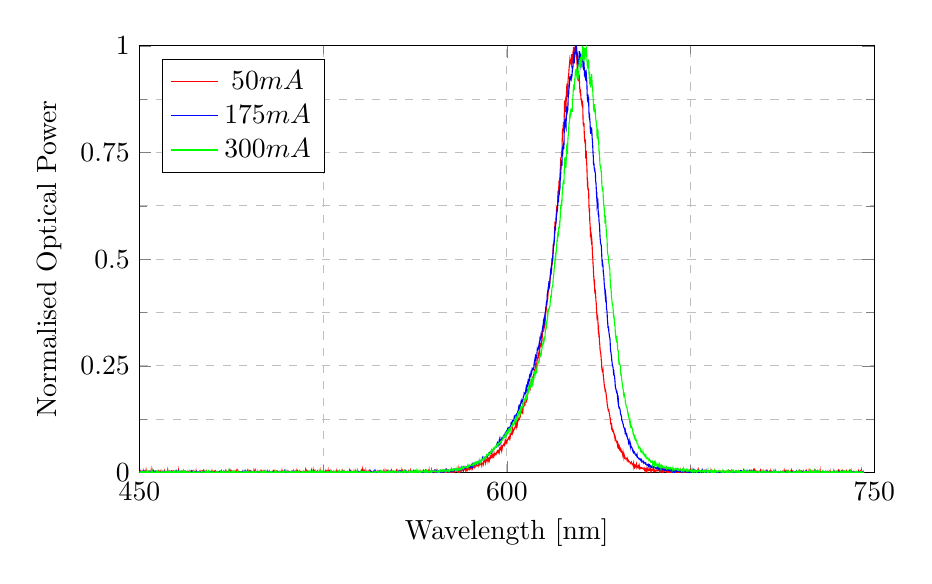
\begin{tikzpicture}

\begin{axis}[
    %title={Temperature dependence of CuSO$_4\cdot$5H$_2$O solubility},
    xlabel={Wavelength [nm]},
    ylabel={Normalised Optical Power},
    height=7cm,
    width=0.9\textwidth,
    xmin=450, xmax=750,
    ymin=0, ymax=1,
    xtick={450, 600, 750},
    ytick={0.0, 0.25, 0.5, 0.75, 1.0},
    % xtick={610, 620, 630, 640, 650, 660},
    % ytick={0.5, 0.75, 1.0},
    legend pos=north west,
    ymajorgrids=true,
    yminorgrids=true,
    xmajorgrids=true,
    xminorgrids=true,
    minor tick num=1,
    grid style=dashed,
]

\addplot[color=red]
  coordinates {
  (321.5116882,0.0006542079270406207)
  (321.6192017,0.0004690547159199363)
  (321.7267151,0.003653689484990084)
  (321.834259,0.0031722911874207307)
  (321.941803,-0.001086232000806948)
  (322.0493164,0.00024687091395480474)
  (322.1568909,-0.0007529562720283499)
  (322.2644348,9.874836429478485e-05)
  (322.3720093,0.0006171772848870119)
  (322.4795837,0.0031352605967526035)
  (322.5871582,0.0023205865705809717)
  (322.6947327,-0.0008640481473563349)
  (322.8023376,0.0015059125442330199)
  (322.9099426,0.0023946477519172257)
  (323.0175476,-0.00038264990127246285)
  (323.1251526,-0.0005678031122168271)
  (323.2327881,0.0018391882730116182)
  (323.3404236,0.0003949934571791394)
  (323.4480591,0.002913076846449274)
  (323.5556946,9.874836429478485e-05)
  (323.6633606,0.0006171772848870119)
  (323.7710266,-0.0015305996047372114)
  (323.8786926,0.00024687091395480474)
  (323.9863586,-4.9374182138576416e-05)
  (324.0940552,0.005505221493931245)
  (324.2017517,0.0004320240737663275)
  (324.3094482,0.0003949934571791394)
  (324.4171448,-0.001900905924712897)
  (324.5248718,0.0030982300060844767)
  (324.6325989,9.874836429478485e-05)
  (324.7403259,0.0009134223713356812)
  (324.848053,-0.001382477138564779)
  (324.9558105,0.0022835559799128445)
  (325.0635681,0.002098402820277642)
  (325.1713257,0.003394475144018628)
  (325.2790833,0.00154294323769579)
  (325.3868713,0.0023946477519172257)
  (325.4946594,-0.0006048337545467561)
  (325.6024475,0.001765127091675364)
  (325.7102356,-0.0005307724700632183)
  (325.8180542,0.0022835559799128445)
  (325.9258728,-0.001197323876134933)
  (326.0336914,0.0022465253892447177)
  (326.14151,0.00035796281484921043)
  (326.2493591,0.0020613720233149477)
  (326.3571777,0.0006912385691942295)
  (326.4650269,0.001617004522179328)
  (326.5729065,-0.0006418643967003649)
  (326.6807556,0.0011726368154544216)
  (326.7886353,-0.0005678031122168271)
  (326.8965149,0.0013577899752659443)
  (327.0043945,0.003394475144018628)
  (327.1123047,-0.0016416915826835193)
  (327.2202148,-0.0020860592888794654)
  (327.328125,0.0028390154588184527)
  (327.4360352,6.171772848870119e-05)
  (327.5439758,0.0018762188636797452)
  (327.651886,0.0010615449401264365)
  (327.7598267,0.0022835559799128445)
  (327.8677979,0.0015059125442330199)
  (327.9757385,0.002172464001613896)
  (328.0837097,0.0007282692115241584)
  (328.1916809,0.0007652998023686057)
  (328.2996521,0.0007282692115241584)
  (328.4076538,2.468709107810422e-05)
  (328.515625,0.0006912385691942295)
  (328.6236267,0.001024514246663666)
  (328.7316589,0.0002098402716248758)
  (328.8396606,0.0012837287934007297)
  (328.9476929,0.0009504529621801285)
  (329.0557251,0.00017280964230737336)
  (329.1637573,0.00017280964230737336)
  (329.2717896,0.002727923480519504)
  (329.3798523,-0.000975140125478963)
  (329.487915,0.0002098402716248758)
  (329.5959778,-0.0014195077294092264)
  (329.704071,-0.00012343545695977034)
  (329.8121338,-0.00038264990127246285)
  (329.9202271,0.0004320240737663275)
  (330.0283203,0.0006171772848870119)
  (330.1364441,0.000543116000403474)
  (330.2445374,2.468709107810422e-05)
  (330.3526611,0.0020613720233149477)
  (330.4607849,0.0009874836556428989)
  (330.5689392,-0.001049201409786181)
  (330.677063,-0.0006418643967003649)
  (330.7852173,-0.0003456192846852748)
  (330.8933716,0.0004690547159199363)
  (331.0015564,0.0016540351130237751)
  (331.1097107,-0.0006418643967003649)
  (331.2178955,-0.0006788949877211323)
  (331.3260803,0.002542770320884301)
  (331.4342651,0.003246352575051552)
  (331.5424805,2.468709107810422e-05)
  (331.6506958,-0.0007529562720283499)
  (331.7589111,-0.0007899869143582788)
  (331.8671265,-0.0012713851606184709)
  (331.9753723,-0.0007159256298747411)
  (332.0835876,9.874836429478485e-05)
  (332.1918335,0.0015059125442330199)
  (332.3001099,0.0009504529621801285)
  (332.4083557,-0.0023082430409459963)
  (332.5166321,-0.0007159256298747411)
  (332.6249084,-0.0015305996047372114)
  (332.7331848,-0.0004196805434260717)
  (332.8414612,0.0025798011178469957)
  (332.9497681,0.004579455283166097)
  (333.058075,0.0009874836556428989)
  (333.1663818,0.00017280964230737336)
  (333.2747192,-0.0011232626942697186)
  (333.3830261,-0.0004196805434260717)
  (333.4913635,0.000543116000403474)
  (333.5997009,0.0009874836556428989)
  (333.7080688,-0.0016787221737042867)
  (333.8164368,0.0012096675090935121)
  (333.9247742,-0.0012343545695977036)
  (334.0331726,0.0019873108419786937)
  (334.1415405,-0.0013454464449256887)
  (334.2499084,0.0006542079270406207)
  (334.3583069,9.874836429478485e-05)
  (334.4667053,0.00017280964230737336)
  (334.5751343,0.0010985755309708839)
  (334.6835327,0.0011726368154544216)
  (334.7919617,0.00024687091395480474)
  (334.9003906,0.0012837287934007297)
  (335.0088196,-0.000975140125478963)
  (335.1172791,0.0017280962948889897)
  (335.2257385,0.0004690547159199363)
  (335.334198,-0.0005307724700632183)
  (335.4426575,0.0008763917803149138)
  (335.5511169,0.0006912385691942295)
  (335.6596069,-0.0018268447433766428)
  (335.7680969,0.002172464001613896)
  (335.8765869,-0.0011232626942697186)
  (335.9851074,0.0013577899752659443)
  (336.0935974,-0.0010121707163234103)
  (336.2021179,0.0013577899752659443)
  (336.3106384,0.0008393610868521434)
  (336.4191895,0.0016540351130237751)
  (336.5277405,-0.0004196805434260717)
  (336.636261,-0.002271212448514668)
  (336.7448425,2.468709107810422e-05)
  (336.8533936,0.0022835559799128445)
  (336.9619446,0.006468018089069953)
  (337.0705261,0.00028390155610841353)
  (337.1791077,0.0007652998023686057)
  (337.2877197,-0.0011602932851141657)
  (337.3963013,-0.0009381094318398726)
  (337.5049133,0.0007652998023686057)
  (337.6135254,-0.0015305996047372114)
  (337.7221375,0.00154294323769579)
  (337.83078,0.001617004522179328)
  (337.9394226,9.874836429478485e-05)
  (338.0480652,-0.0012343545695977036)
  (338.1567078,0.0006542079270406207)
  (338.2653503,0.0002098402716248758)
  (338.3740234,-0.0008270175565118876)
  (338.4826965,-0.0005678031122168271)
  (338.5913696,-0.001049201409786181)
  (338.7000427,-0.0004937418279096095)
  (338.8087463,-8.640482115368668e-05)
  (338.91745,0.0018391882730116182)
  (339.0261536,0.0004690547159199363)
  (339.1348572,-0.0018268447433766428)
  (339.2435913,0.00024687091395480474)
  (339.3523254,-0.002345273631614124)
  (339.4610596,0.002357617161249099)
  (339.5697937,-0.0001974967285895697)
  (339.6785583,0.0022465253892447177)
  (339.787323,-0.0007159256298747411)
  (339.8960876,0.001765127091675364)
  (340.0048523,-4.9374182138576416e-05)
  (340.1136169,-0.0015305996047372114)
  (340.2224121,-0.0001974967285895697)
  (340.3312073,0.00361665868802739)
  (340.4400024,0.0026538622991832497)
  (340.5488281,6.171772848870119e-05)
  (340.6576233,0.0005801466425570829)
  (340.766449,0.002542770320884301)
  (340.8752747,-0.001086232000806948)
  (340.9841309,0.0006542079270406207)
  (341.0929565,-0.001197323876134933)
  (341.2018127,0.0019132496606424393)
  (341.3106689,0.0009874836556428989)
  (341.4195557,-0.00045671118557968053)
  (341.5284119,0.001765127091675364)
  (341.6372986,0.0025798011178469957)
  (341.7461853,-0.001086232000806948)
  (341.855072,-0.0007899869143582788)
  (341.9639893,-0.0017898141509453144)
  (342.0729065,0.0022835559799128445)
  (342.1818237,0.0005801466425570829)
  (342.290741,0.0012466980999379592)
  (342.3996582,0.0014688819532122524)
  (342.508606,0.0006542079270406207)
  (342.6175537,2.468709107810422e-05)
  (342.7265015,0.0012096675090935121)
  (342.8354492,0.0013577899752659443)
  (342.9444275,-0.0006048337545467561)
  (343.0534058,-0.0007529562720283499)
  (343.162384,0.003320413756387806)
  (343.2713623,0.0006912385691942295)
  (343.3803711,0.003024168618453655)
  (343.4893799,-0.00012343545695977034)
  (343.5983887,0.0002098402716248758)
  (343.7073975,-0.002271212448514668)
  (343.8164063,-0.0026044881771169464)
  (343.9254456,0.0005060853580735451)
  (344.0344849,0.0007282692115241584)
  (344.1435242,6.171772848870119e-05)
  (344.252594,0.0013948206689050348)
  (344.3616333,0.0001357790001008685)
  (344.4707031,-0.001197323876134933)
  (344.5798035,-0.0019379367199123898)
  (344.6888733,-0.0008640481473563349)
  (344.7979736,-0.0017898141509453144)
  (344.9070435,0.0018391882730116182)
  (345.0161438,-0.0016416915826835193)
  (345.1252747,0.0023205865705809717)
  (345.234375,0.0008023304445222145)
  (345.3435059,0.0015799738285402374)
  (345.4526367,0.0008393610868521434)
  (345.5617676,-0.0008640481473563349)
  (345.670929,0.0024316785488799203)
  (345.7800598,-0.0023082430409459963)
  (345.8892212,-0.001197323876134933)
  (345.9984131,0.0008393610868521434)
  (346.1075745,0.001024514246663666)
  (346.2167664,-0.0016416915826835193)
  (346.3259277,0.0018762188636797452)
  (346.4351501,0.0018391882730116182)
  (346.544342,2.468709107810422e-05)
  (346.6535339,0.00154294323769579)
  (346.7627563,0.00028390155610841353)
  (346.8719788,-0.001382477138564779)
  (346.9812317,-0.0009381094318398726)
  (347.0904541,-4.9374182138576416e-05)
  (347.199707,-0.001604660889220749)
  (347.30896,0.005097884377698145)
  (347.4182129,-0.0007899869143582788)
  (347.5274658,0.00024687091395480474)
  (347.6367493,0.0005801466425570829)
  (347.7460327,0.0018391882730116182)
  (347.8553162,0.0018762188636797452)
  (347.9645996,0.0009504529621801285)
  (348.0739136,0.0019132496606424393)
  (348.1832275,0.0009874836556428989)
  (348.2925415,0.0008763917803149138)
  (348.4018555,0.0022835559799128445)
  (348.5112,0.0017280962948889897)
  (348.6205139,0.003246352575051552)
  (348.7298584,0.0012466980999379592)
  (348.8392029,0.002542770320884301)
  (348.9485779,9.874836429478485e-05)
  (349.0579529,0.0014318512597494822)
  (349.1672974,-0.0003456192846852748)
  (349.2767029,-0.0007899869143582788)
  (349.3860779,-0.0008270175565118876)
  (349.4954834,-0.000271558000201737)
  (349.6048584,0.0019873108419786937)
  (349.7142639,0.0007282692115241584)
  (349.8237,0.0033574443470559333)
  (349.9331055,-0.000271558000201737)
  (350.0425415,0.00028390155610841353)
  (350.1519775,0.0014688819532122524)
  (350.2614136,0.0004320240737663275)
  (350.3708496,0.0007282692115241584)
  (350.4803162,0.0013577899752659443)
  (350.5897827,0.0009134223713356812)
  (350.6992493,0.0003209321984383425)
  (350.8087158,-0.0003085886423553459)
  (350.9182129,-0.00038264990127246285)
  (351.02771,-0.00045671118557968053)
  (351.137207,-0.0006048337545467561)
  (351.2467041,-0.00038264990127246285)
  (351.3562317,0.0013948206689050348)
  (351.4657288,0.001802157682343491)
  (351.5752563,0.00017280964230737336)
  (351.6847839,0.005283037537333348)
  (351.794342,0.0007652998023686057)
  (351.9038696,0.0004320240737663275)
  (352.0134277,0.0003949934571791394)
  (352.1229858,-0.0008640481473563349)
  (352.2325745,0.0018762188636797452)
  (352.3421326,0.002357617161249099)
  (352.4517212,6.171772848870119e-05)
  (352.5613098,0.0012837287934007297)
  (352.6708984,0.003394475144018628)
  (352.7805176,0.0009134223713356812)
  (352.8901062,0.0007652998023686057)
  (352.9997253,-0.0012713851606184709)
  (353.1093445,0.0020243414326468205)
  (353.2189941,0.0013577899752659443)
  (353.3286133,-0.00045671118557968053)
  (353.4382629,-0.00016046609918390724)
  (353.5479126,-0.00016046609918390724)
  (353.6575928,0.0030611992091217825)
  (353.7672424,0.0015059125442330199)
  (353.8769226,0.0022094945922820236)
  (353.9866028,-0.0021230898795475926)
  (354.096283,0.002172464001613896)
  (354.2059631,-0.0011232626942697186)
  (354.3156738,0.0006912385691942295)
  (354.4253845,0.0006171772848870119)
  (354.5350952,0.0013577899752659443)
  (354.6448059,-0.0017157528671670572)
  (354.7545471,0.0009874836556428989)
  (354.8642883,0.0003949934571791394)
  (354.9740295,0.0012096675090935121)
  (355.0837708,-0.00045671118557968053)
  (355.193512,0.0015799738285402374)
  (355.3032837,6.171772848870119e-05)
  (355.4130554,0.0024316785488799203)
  (355.5228271,0.0016540351130237751)
  (355.6325989,0.0013207593844214971)
  (355.7424011,-0.001049201409786181)
  (355.8522034,-0.00038264990127246285)
  (355.9620056,0.002098402820277642)
  (356.0718079,0.0002098402716248758)
  (356.1816406,0.0020613720233149477)
  (356.2914429,-4.9374182138576416e-05)
  (356.4012756,0.0004690547159199363)
  (356.5111084,0.00024687091395480474)
  (356.6209717,0.0028390154588184527)
  (356.730835,0.004801639239763994)
  (356.8406677,0.0016540351130237751)
  (356.950531,0.002135433410945769)
  (357.0604248,0.0006912385691942295)
  (357.1702881,0.0014688819532122524)
  (357.2801819,0.00028390155610841353)
  (357.3900757,0.0016910657038682224)
  (357.4999695,0.0005801466425570829)
  (357.6098938,-0.0003085886423553459)
  (357.7197876,0.0006542079270406207)
  (357.8297119,0.0016910657038682224)
  (357.9396362,0.000543116000403474)
  (358.0495911,0.0018762188636797452)
  (358.1595154,0.0005801466425570829)
  (358.2694702,-0.0008640481473563349)
  (358.379425,-0.001900905924712897)
  (358.4893799,0.0008763917803149138)
  (358.5993652,-4.9374182138576416e-05)
  (358.7093201,0.0023205865705809717)
  (358.8193054,0.0025798011178469957)
  (358.9292908,0.0002098402716248758)
  (359.0393066,0.00017280964230737336)
  (359.149292,0.0027649542774821983)
  (359.2593079,9.874836429478485e-05)
  (359.3693237,-0.0007529562720283499)
  (359.4793396,-0.002160120471978921)
  (359.589386,0.00035796281484921043)
  (359.6994019,-0.0014195077294092264)
  (359.8094482,-0.000271558000201737)
  (359.9194946,0.003024168618453655)
  (360.0295715,0.0009504529621801285)
  (360.1396179,-0.0017157528671670572)
  (360.2496948,0.0008393610868521434)
  (360.3597717,-4.9374182138576416e-05)
  (360.4698486,0.0009134223713356812)
  (360.5799561,0.0009134223713356812)
  (360.690033,-0.00012343545695977034)
  (360.8001404,-0.0014195077294092264)
  (360.9102478,0.0004690547159199363)
  (361.0203857,0.0014688819532122524)
  (361.1304932,0.0011726368154544216)
  (361.2406311,0.0006542079270406207)
  (361.350769,0.0024316785488799203)
  (361.460907,-0.0001974967285895697)
  (361.5710754,0.00035796281484921043)
  (361.6812439,-0.00016046609918390724)
  (361.7914124,-0.0016787221737042867)
  (361.9015808,0.0009874836556428989)
  (362.0117493,0.0033574443470559333)
  (362.1219482,0.0005060853580735451)
  (362.2321167,0.005468190696968551)
  (362.3423157,-0.0009381094318398726)
  (362.4525452,-0.0011602932851141657)
  (362.5627441,-0.0008270175565118876)
  (362.6729736,0.003468536325354882)
  (362.7832031,-1.2343545535525704e-05)
  (362.8934326,-0.00038264990127246285)
  (363.0036621,-0.00038264990127246285)
  (363.1139221,-0.0004196805434260717)
  (363.2241821,-0.0004937418279096095)
  (363.3344421,0.0005060853580735451)
  (363.4447021,-0.0004937418279096095)
  (363.5549622,0.0025798011178469957)
  (363.6652527,0.00028390155610841353)
  (363.7755432,0.003024168618453655)
  (363.8858337,0.0016910657038682224)
  (363.9961243,0.0025057397302161743)
  (364.1064453,0.0010615449401264365)
  (364.2167664,0.001024514246663666)
  (364.3270874,0.00024687091395480474)
  (364.4374084,-0.0009381094318398726)
  (364.5477295,0.0009504529621801285)
  (364.6580811,0.0009134223713356812)
  (364.7684326,-0.0017157528671670572)
  (364.8787842,0.0016910657038682224)
  (364.9891357,-0.000975140125478963)
  (365.0995178,0.0006542079270406207)
  (365.2098999,-0.0017527835608061478)
  (365.320282,0.001024514246663666)
  (365.4306641,-0.0008270175565118876)
  (365.5410461,0.0003949934571791394)
  (365.6514587,-0.001493569013892764)
  (365.7618713,0.001802157682343491)
  (365.8722839,-0.0004937418279096095)
  (365.9826965,-0.0011232626942697186)
  (366.0931396,0.0005801466425570829)
  (366.2035522,0.003653689484990084)
  (366.3139954,6.171772848870119e-05)
  (366.4244385,0.0003209321984383425)
  (366.5349121,0.0006171772848870119)
  (366.6453552,-0.00016046609918390724)
  (366.7558289,0.0010985755309708839)
  (366.8663025,0.0022465253892447177)
  (366.9768066,-0.0009010788409954254)
  (367.0872803,0.0007282692115241584)
  (367.1977844,-0.0012343545695977036)
  (367.3082886,-0.0009381094318398726)
  (367.4187927,0.0006912385691942295)
  (367.5292969,0.002172464001613896)
  (367.6398315,-0.00038264990127246285)
  (367.7503662,0.00017280964230737336)
  (367.8609009,0.0032833831657196793)
  (367.9714355,-0.001049201409786181)
  (368.0819702,-0.0009010788409954254)
  (368.1925354,0.0012466980999379592)
  (368.3031006,-0.0004196805434260717)
  (368.4136658,-0.0012343545695977036)
  (368.524231,-0.001049201409786181)
  (368.6348267,-0.00016046609918390724)
  (368.7453918,0.00035796281484921043)
  (368.8559875,0.001024514246663666)
  (368.9666138,0.0015799738285402374)
  (369.0772095,0.00028390155610841353)
  (369.1878357,0.0002098402716248758)
  (369.2984619,-8.640482115368668e-05)
  (369.4090881,-0.0002345273580481282)
  (369.5197144,0.0005801466425570829)
  (369.6303406,-0.0011232626942697186)
  (369.7409973,0.0022094945922820236)
  (369.8516541,0.0006542079270406207)
  (369.9623108,-0.0009381094318398726)
  (370.0729675,-0.0003085886423553459)
  (370.1836548,0.000543116000403474)
  (370.294342,-0.0016416915826835193)
  (370.4050293,0.001765127091675364)
  (370.5157166,0.0015799738285402374)
  (370.6264038,0.0006542079270406207)
  (370.7371216,0.0002098402716248758)
  (370.8478394,0.0019873108419786937)
  (370.9585571,-0.0017157528671670572)
  (371.0692749,0.0023205865705809717)
  (371.1800232,-1.2343545535525704e-05)
  (371.2907715,0.0005060853580735451)
  (371.4015198,0.0014688819532122524)
  (371.5122681,-8.640482115368668e-05)
  (371.6230164,0.0013577899752659443)
  (371.7337952,0.0028760460494865795)
  (371.8445435,0.00017280964230737336)
  (371.9553223,9.874836429478485e-05)
  (372.0661316,6.171772848870119e-05)
  (372.1769104,0.002542770320884301)
  (372.2877197,-0.001086232000806948)
  (372.3985291,-0.0004937418279096095)
  (372.5093384,0.0028760460494865795)
  (372.6201477,0.0022835559799128445)
  (372.7309875,0.001617004522179328)
  (372.8417969,0.0008023304445222145)
  (372.9526367,-0.0020119979030118456)
  (373.0635071,0.0028390154588184527)
  (373.1743469,0.0009504529621801285)
  (373.2852173,0.001024514246663666)
  (373.3960571,0.0010615449401264365)
  (373.5069275,0.0010615449401264365)
  (373.6178284,0.00028390155610841353)
  (373.7286987,0.0012466980999379592)
  (373.8395996,-0.0009010788409954254)
  (373.9505005,0.003394475144018628)
  (374.0614014,-0.0002345273580481282)
  (374.1723022,0.0017280962948889897)
  (374.2832336,-0.0037894685243221845)
  (374.3941345,-0.00012343545695977034)
  (374.5050659,0.0011726368154544216)
  (374.6159973,-0.0011232626942697186)
  (374.7269592,0.002135433410945769)
  (374.8378906,-0.0004196805434260717)
  (374.9488525,0.00017280964230737336)
  (375.0598145,-0.00038264990127246285)
  (375.1707764,0.0015799738285402374)
  (375.2817688,-0.0009010788409954254)
  (375.3927612,6.171772848870119e-05)
  (375.5037231,0.0012837287934007297)
  (375.6147156,0.0022465253892447177)
  (375.7257385,0.00035796281484921043)
  (375.836731,6.171772848870119e-05)
  (375.9477539,0.004653516877091485)
  (376.0587769,-0.0007529562720283499)
  (376.1697998,0.0016540351130237751)
  (376.2808228,0.0005801466425570829)
  (376.3918762,0.0009504529621801285)
  (376.5029297,0.0004320240737663275)
  (376.6139832,-0.0006418643967003649)
  (376.7250366,-0.0006048337545467561)
  (376.8360901,0.0016910657038682224)
  (376.9471741,-0.002530426791249326)
  (377.0582581,0.0007652998023686057)
  (377.169342,0.0022835559799128445)
  (377.280426,0.00028390155610841353)
  (377.3915405,-0.0018268447433766428)
  (377.5026245,0.000543116000403474)
  (377.613739,-0.000975140125478963)
  (377.7248535,0.0012837287934007297)
  (377.8359985,-0.00012343545695977034)
  (377.947113,0.002357617161249099)
  (378.0582581,0.0008393610868521434)
  (378.1694031,0.0011726368154544216)
  (378.2805481,-0.0005678031122168271)
  (378.3916931,0.0020613720233149477)
  (378.5028687,0.0006171772848870119)
  (378.6140442,0.0004690547159199363)
  (378.7252197,0.0008023304445222145)
  (378.8363953,0.0014318512597494822)
  (378.9475708,-0.001604660889220749)
  (379.0587769,0.002727923480519504)
  (379.1699829,-1.2343545535525704e-05)
  (379.281189,0.0019132496606424393)
  (379.392395,0.001024514246663666)
  (379.5036316,-0.0013084158540812413)
  (379.6148376,-0.0004196805434260717)
  (379.7260742,-0.00012343545695977034)
  (379.8373108,-0.0008270175565118876)
  (379.9485779,0.0015059125442330199)
  (380.0598145,-0.0003085886423553459)
  (380.1710815,0.0011726368154544216)
  (380.2823486,-0.0004937418279096095)
  (380.3936157,0.0009874836556428989)
  (380.5048828,0.00017280964230737336)
  (380.6161804,0.002987138027785528)
  (380.727478,0.0013948206689050348)
  (380.8387756,0.0009134223713356812)
  (380.9500732,0.0005801466425570829)
  (381.0613708,0.0012837287934007297)
  (381.172699,0.001617004522179328)
  (381.2840271,-0.0003085886423553459)
  (381.3953552,9.874836429478485e-05)
  (381.5066833,-0.0004196805434260717)
  (381.618042,0.002616831708515123)
  (381.7293701,0.0012096675090935121)
  (381.8407288,0.0006912385691942295)
  (381.9520874,0.0014318512597494822)
  (382.0634766,0.0017280962948889897)
  (382.1748352,0.0014318512597494822)
  (382.2862244,0.0013948206689050348)
  (382.3976135,0.003764781463289033)
  (382.5090027,0.0009874836556428989)
  (382.6203918,0.004394302123530895)
  (382.7318115,0.0016540351130237751)
  (382.8432007,0.003727750666326339)
  (382.9546204,0.00035796281484921043)
  (383.0660706,0.0012466980999379592)
  (383.1774902,0.0017280962948889897)
  (383.2889099,0.0024316785488799203)
  (383.4003601,0.0015799738285402374)
  (383.5118103,0.002542770320884301)
  (383.6232605,0.0008023304445222145)
  (383.7347412,-0.0002345273580481282)
  (383.8461914,0.0007652998023686057)
  (383.9576721,0.0005801466425570829)
  (384.0691528,-0.001604660889220749)
  (384.1806641,0.0015059125442330199)
  (384.2921448,-0.0013084158540812413)
  (384.403656,0.0016910657038682224)
  (384.5151672,-0.0002345273580481282)
  (384.6266785,-0.0017898141509453144)
  (384.7381897,-0.002826671929183477)
  (384.8497009,0.0012096675090935121)
  (384.9612427,-0.0014195077294092264)
  (385.0727844,0.0008023304445222145)
  (385.1843262,-0.000271558000201737)
  (385.2958679,0.0011356062246099742)
  (385.4074402,0.0008393610868521434)
  (385.5190125,0.002357617161249099)
  (385.6305542,-0.0026415187695482747)
  (385.742157,0.0028760460494865795)
  (385.8537292,-0.0023082430409459963)
  (385.9653015,-0.0010121707163234103)
  (386.0769043,0.0014318512597494822)
  (386.1885071,0.0025057397302161743)
  (386.3001099,0.0003949934571791394)
  (386.4117432,-0.00045671118557968053)
  (386.5233459,-0.00012343545695977034)
  (386.6349792,-8.640482115368668e-05)
  (386.7466125,0.0016910657038682224)
  (386.8582458,0.0009134223713356812)
  (386.9699097,-0.000271558000201737)
  (387.081543,0.0018762188636797452)
  (387.1932068,0.0010615449401264365)
  (387.3048706,-0.0013084158540812413)
  (387.4165344,-0.0001974967285895697)
  (387.5282288,-0.000975140125478963)
  (387.6398926,9.874836429478485e-05)
  (387.7515869,0.001765127091675364)
  (387.8632813,0.0004690547159199363)
  (387.9749756,0.0011356062246099742)
  (388.0867004,0.0008393610868521434)
  (388.1983948,9.874836429478485e-05)
  (388.3101196,-0.0013084158540812413)
  (388.4218445,0.0009874836556428989)
  (388.5335693,-0.0009381094318398726)
  (388.6453247,0.0006912385691942295)
  (388.7570801,-0.000271558000201737)
  (388.8688049,-0.0007899869143582788)
  (388.9805603,0.0011726368154544216)
  (389.0923462,0.000543116000403474)
  (389.2041016,0.0014318512597494822)
  (389.3158875,0.0006171772848870119)
  (389.4276733,0.001765127091675364)
  (389.5394592,0.0023946477519172257)
  (389.6512451,0.00028390155610841353)
  (389.7630615,-0.0004937418279096095)
  (389.8748474,-0.0006418643967003649)
  (389.9866638,0.0004690547159199363)
  (390.0984802,-0.001382477138564779)
  (390.2103271,0.004135087782559438)
  (390.3221436,0.0004690547159199363)
  (390.4339905,0.001802157682343491)
  (390.5458374,0.001024514246663666)
  (390.6576843,0.0031722911874207307)
  (390.7695313,-0.0011602932851141657)
  (390.8814087,-0.0013454464449256887)
  (390.9932556,-0.0015676302983763017)
  (391.1051331,0.0019132496606424393)
  (391.2170105,0.0016540351130237751)
  (391.3289185,0.0009874836556428989)
  (391.4407959,0.0006542079270406207)
  (391.5527039,0.0008023304445222145)
  (391.6646118,-0.0011602932851141657)
  (391.7765198,0.0017280962948889897)
  (391.8884277,0.0008393610868521434)
  (392.0003662,0.0003949934571791394)
  (392.1123047,0.0018391882730116182)
  (392.2242432,0.0013577899752659443)
  (392.3361816,0.000543116000403474)
  (392.4481201,-0.0015305996047372114)
  (392.5600891,0.0004690547159199363)
  (392.6720276,0.003320413756387806)
  (392.7839966,-0.0001974967285895697)
  (392.8959961,0.002172464001613896)
  (393.0079651,0.0009504529621801285)
  (393.1199341,0.003690720281952779)
  (393.2319336,-0.0007159256298747411)
  (393.3439331,0.0004690547159199363)
  (393.4559326,-0.000271558000201737)
  (393.5679626,0.00024687091395480474)
  (393.6799622,0.0025057397302161743)
  (393.7919922,0.003912903825961541)
  (393.9040222,-1.2343545535525704e-05)
  (394.0160522,0.003690720281952779)
  (394.1280823,0.000543116000403474)
  (394.2401428,0.0006542079270406207)
  (394.3522034,0.003468536325354882)
  (394.4642639,0.004468363306630351)
  (394.5763245,-0.0005678031122168271)
  (394.688385,-0.0018268447433766428)
  (394.8004761,0.0025798011178469957)
  (394.9125671,0.0011726368154544216)
  (395.0246277,0.0012096675090935121)
  (395.1367493,0.0006912385691942295)
  (395.2488403,0.0018391882730116182)
  (395.3609619,0.0012837287934007297)
  (395.473053,0.00035796281484921043)
  (395.5851746,-4.9374182138576416e-05)
  (395.6972961,-0.0008640481473563349)
  (395.8094482,0.001617004522179328)
  (395.9215698,6.171772848870119e-05)
  (396.0337219,0.0009134223713356812)
  (396.145874,0.0006912385691942295)
  (396.2580261,0.0016910657038682224)
  (396.3702087,0.000543116000403474)
  (396.4823608,-0.00038264990127246285)
  (396.5945435,0.002542770320884301)
  (396.7067261,0.002135433410945769)
  (396.8189087,0.00024687091395480474)
  (396.9310913,0.0011356062246099742)
  (397.0433044,-0.0005678031122168271)
  (397.1555176,0.0023205865705809717)
  (397.2677002,0.0006542079270406207)
  (397.3799438,0.0009504529621801285)
  (397.492157,-0.0010121707163234103)
  (397.6043701,-0.0015305996047372114)
  (397.7166138,0.0009874836556428989)
  (397.8288574,0.0018762188636797452)
  (397.9411011,0.0013207593844214971)
  (398.0533752,0.0007652998023686057)
  (398.1656189,0.0018391882730116182)
  (398.2778931,0.0028760460494865795)
  (398.3901672,0.001617004522179328)
  (398.5024414,0.0023205865705809717)
  (398.6147156,-0.001900905924712897)
  (398.7270203,-0.0005307724700632183)
  (398.8392944,0.0009134223713356812)
  (398.9515991,0.0016910657038682224)
  (399.0639038,-0.0013084158540812413)
  (399.176239,9.874836429478485e-05)
  (399.2885437,-0.00045671118557968053)
  (399.4008789,0.004801639239763994)
  (399.5132141,0.0009134223713356812)
  (399.6255493,0.0006912385691942295)
  (399.7378845,-0.0001974967285895697)
  (399.8502502,-0.00045671118557968053)
  (399.9625854,0.0006912385691942295)
  (400.0749512,0.002357617161249099)
  (400.1873169,0.0019502802513105667)
  (400.2996826,0.0006542079270406207)
  (400.4120789,0.0020613720233149477)
  (400.5244446,0.001024514246663666)
  (400.6368408,0.0007652998023686057)
  (400.7492371,-0.0020490284936799724)
  (400.8616638,0.0019502802513105667)
  (400.9740601,-0.000975140125478963)
  (401.0864868,0.00024687091395480474)
  (401.1989136,-0.001382477138564779)
  (401.3113403,-0.0007159256298747411)
  (401.4237671,-8.640482115368668e-05)
  (401.5361938,0.0026908928898513773)
  (401.6486511,-0.0011602932851141657)
  (401.7611084,-0.0019749673105805172)
  (401.8735657,0.0013948206689050348)
  (401.9860229,-0.0004196805434260717)
  (402.0984802,-0.00038264990127246285)
  (402.210968,0.0010615449401264365)
  (402.3234558,0.0008023304445222145)
  (402.4359436,0.0017280962948889897)
  (402.5484314,-0.0007529562720283499)
  (402.6609192,0.000543116000403474)
  (402.7734375,-0.0015305996047372114)
  (402.8859253,-0.00045671118557968053)
  (402.9984436,-0.0009381094318398726)
  (403.1109619,-0.0023082430409459963)
  (403.2235107,0.0007282692115241584)
  (403.3360291,-0.0005678031122168271)
  (403.4485779,0.001765127091675364)
  (403.5611267,-0.0016787221737042867)
  (403.6736755,-0.0003456192846852748)
  (403.7862244,-0.0005678031122168271)
  (403.8988037,0.0016540351130237751)
  (404.0113831,-0.0026785493602164015)
  (404.1239319,-1.2343545535525704e-05)
  (404.2365417,-0.0006048337545467561)
  (404.3491211,0.00028390155610841353)
  (404.4617004,-0.001493569013892764)
  (404.5743103,-0.003715407341222729)
  (404.6869202,0.001617004522179328)
  (404.79953,-0.0003456192846852748)
  (404.9121399,-0.0013454464449256887)
  (405.0247803,0.0030982300060844767)
  (405.1373901,-1.2343545535525704e-05)
  (405.2500305,0.0006542079270406207)
  (405.3626709,0.0012096675090935121)
  (405.4753113,0.0015059125442330199)
  (405.5879822,0.0015799738285402374)
  (405.7006226,-0.0007529562720283499)
  (405.8132935,0.0026538622991832497)
  (405.9259644,0.0015799738285402374)
  (406.0386353,6.171772848870119e-05)
  (406.1513062,0.002357617161249099)
  (406.2640076,0.0005801466425570829)
  (406.376709,0.0013948206689050348)
  (406.4894104,6.171772848870119e-05)
  (406.6021118,0.002135433410945769)
  (406.7148132,0.0002098402716248758)
  (406.8275452,0.0028019848681503255)
  (406.9402466,-0.0013084158540812413)
  (407.0529785,0.0003209321984383425)
  (407.1657104,-0.0005307724700632183)
  (407.2784729,0.0004690547159199363)
  (407.3912048,-0.0027526107460840218)
  (407.5039673,-0.0002345273580481282)
  (407.6167297,-8.640482115368668e-05)
  (407.7294922,0.0012096675090935121)
  (407.8422546,-0.00045671118557968053)
  (407.9550171,-1.2343545535525704e-05)
  (408.0678101,0.0033574443470559333)
  (408.180603,0.0014318512597494822)
  (408.293396,-0.001382477138564779)
  (408.406189,0.00028390155610841353)
  (408.5189819,-0.0014195077294092264)
  (408.6318054,-0.00045671118557968053)
  (408.7446289,0.003209321778088858)
  (408.8574524,0.0010615449401264365)
  (408.9702759,-0.0010121707163234103)
  (409.0830994,0.0014688819532122524)
  (409.1959534,-0.0018268447433766428)
  (409.3087769,-0.0024193350174817434)
  (409.4216309,0.0009134223713356812)
  (409.5344849,-0.0017157528671670572)
  (409.6473694,-0.0020860592888794654)
  (409.7602234,0.0007652998023686057)
  (409.8731079,0.0031722911874207307)
  (409.9859924,0.0003949934571791394)
  (410.098877,0.001024514246663666)
  (410.2117615,-0.0013084158540812413)
  (410.324646,-0.0019749673105805172)
  (410.437561,-0.0008270175565118876)
  (410.5504761,0.0011356062246099742)
  (410.6633911,-0.0017527835608061478)
  (410.7763062,0.0008763917803149138)
  (410.8892212,-0.00038264990127246285)
  (411.0021667,-0.0028637025198516046)
  (411.1151123,0.0022835559799128445)
  (411.2280579,-0.003604315364686982)
  (411.3410034,-0.0012343545695977036)
  (411.453949,9.874836429478485e-05)
  (411.566925,-0.0017157528671670572)
  (411.6798706,0.004616486080128791)
  (411.7928467,0.0017280962948889897)
  (411.9058228,-0.001086232000806948)
  (412.0187988,0.0009504529621801285)
  (412.1318054,-0.0011232626942697186)
  (412.2447815,-0.0012713851606184709)
  (412.3577881,0.0023946477519172257)
  (412.4707947,0.0020243414326468205)
  (412.5838318,-0.00012343545695977034)
  (412.6968384,-0.0006418643967003649)
  (412.8098755,-0.0013454464449256887)
  (412.9228821,0.0018391882730116182)
  (413.0359192,0.0010985755309708839)
  (413.1489563,0.004246179760858387)
  (413.2620239,0.0016910657038682224)
  (413.375061,0.0002098402716248758)
  (413.4881287,-0.005011479460432349)
  (413.6011963,0.004209148963895693)
  (413.7142639,0.0014318512597494822)
  (413.8273315,0.0023946477519172257)
  (413.9404297,-0.0006788949877211323)
  (414.0534973,0.0008763917803149138)
  (414.1665955,2.468709107810422e-05)
  (414.2796936,0.0002098402716248758)
  (414.3927917,0.0015059125442330199)
  (414.5059204,-0.0017527835608061478)
  (414.6190186,0.0006171772848870119)
  (414.7321472,-0.0017898141509453144)
  (414.8452759,-0.000975140125478963)
  (414.9584045,0.0007652998023686057)
  (415.0715332,-0.0007899869143582788)
  (415.1846924,-0.0007159256298747411)
  (415.2978516,9.874836429478485e-05)
  (415.4109802,-0.0002345273580481282)
  (415.5241699,0.0012096675090935121)
  (415.6373291,0.0026538622991832497)
  (415.7504883,0.0011356062246099742)
  (415.863678,0.0004690547159199363)
  (415.9768677,-0.0033451008174209583)
  (416.0900574,-0.0002345273580481282)
  (416.2032471,0.0009134223713356812)
  (416.3164368,0.00028390155610841353)
  (416.429657,0.0016540351130237751)
  (416.5428467,0.0009504529621801285)
  (416.6560669,-0.0018268447433766428)
  (416.7693176,-0.00012343545695977034)
  (416.8825378,-0.0005678031122168271)
  (416.9957581,0.004986792399399197)
  (417.1090088,-0.0003456192846852748)
  (417.2222595,-0.00016046609918390724)
  (417.3355103,0.0011726368154544216)
  (417.448761,0.0004320240737663275)
  (417.5620117,-0.0015305996047372114)
  (417.675293,0.002727923480519504)
  (417.7885742,0.001024514246663666)
  (417.9018555,-0.00016046609918390724)
  (418.0151367,0.002135433410945769)
  (418.128418,0.0011356062246099742)
  (418.2417297,0.0026538622991832497)
  (418.355011,-0.00012343545695977034)
  (418.4683228,0.0008393610868521434)
  (418.5816345,0.0012466980999379592)
  (418.6949768,-0.0016787221737042867)
  (418.8082886,0.0015059125442330199)
  (418.9216309,-0.0020119979030118456)
  (419.0349426,0.0015059125442330199)
  (419.1482849,0.0011356062246099742)
  (419.2616577,0.002616831708515123)
  (419.375,-0.0024933962005811994)
  (419.4883423,0.0014318512597494822)
  (419.6017151,-0.0022341816533151754)
  (419.7150879,0.0006912385691942295)
  (419.8284607,-0.0006048337545467561)
  (419.9418335,0.0010985755309708839)
  (420.0552368,0.0013577899752659443)
  (420.1686401,0.0009134223713356812)
  (420.2820129,0.00154294323769579)
  (420.3954163,0.0013207593844214971)
  (420.5088501,-0.0002345273580481282)
  (420.6222534,0.0005060853580735451)
  (420.7356567,-0.00038264990127246285)
  (420.8490906,0.0007652998023686057)
  (420.9625244,-0.0008270175565118876)
  (421.0759583,-8.640482115368668e-05)
  (421.1893921,0.001765127091675364)
  (421.3028564,0.0015059125442330199)
  (421.4163208,-0.0019749673105805172)
  (421.5297546,-0.0009010788409954254)
  (421.643219,-0.0011232626942697186)
  (421.7567139,0.0011356062246099742)
  (421.8701782,-0.0006418643967003649)
  (421.9836426,0.0018762188636797452)
  (422.0971375,-0.002826671929183477)
  (422.2106323,0.0007652998023686057)
  (422.3241272,9.874836429478485e-05)
  (422.4376526,-0.00012343545695977034)
  (422.5511475,-0.0008640481473563349)
  (422.6646729,0.002172464001613896)
  (422.7781677,0.00154294323769579)
  (422.8916931,0.003394475144018628)
  (423.005249,-0.001382477138564779)
  (423.1187744,0.003024168618453655)
  (423.2323303,-0.0017527835608061478)
  (423.3458557,0.00024687091395480474)
  (423.4594116,0.002135433410945769)
  (423.5729675,0.0018391882730116182)
  (423.686554,0.0015059125442330199)
  (423.8001099,0.00024687091395480474)
  (423.9136963,0.0018762188636797452)
  (424.0272522,-0.002530426791249326)
  (424.1408386,2.468709107810422e-05)
  (424.2544556,0.003320413756387806)
  (424.368042,-0.0021230898795475926)
  (424.4816589,-0.0008270175565118876)
  (424.5952454,0.0007652998023686057)
  (424.7088623,0.0018762188636797452)
  (424.8224792,0.0004320240737663275)
  (424.9360962,0.0011726368154544216)
  (425.0497437,0.00035796281484921043)
  (425.1633606,0.0013207593844214971)
  (425.2770081,-0.005307724598366499)
  (425.3906555,9.874836429478485e-05)
  (425.504303,-0.00038264990127246285)
  (425.617981,-0.0006788949877211323)
  (425.7316284,0.00154294323769579)
  (425.8453064,0.000543116000403474)
  (425.9589844,-0.0001974967285895697)
  (426.0726624,0.0026538622991832497)
  (426.1863403,-0.0004937418279096095)
  (426.3000488,0.004394302123530895)
  (426.4137268,0.0002098402716248758)
  (426.5274353,-4.9374182138576416e-05)
  (426.6411438,0.0002098402716248758)
  (426.7548523,-0.0003085886423553459)
  (426.8685608,-0.0003456192846852748)
  (426.9822998,0.0015799738285402374)
  (427.0960083,-0.0005678031122168271)
  (427.2097473,-0.0005307724700632183)
  (427.3234863,0.0018391882730116182)
  (427.4372253,0.0008023304445222145)
  (427.5509949,-0.0023082430409459963)
  (427.6647339,0.0017280962948889897)
  (427.7785034,0.0006542079270406207)
  (427.8922729,0.0022835559799128445)
  (428.0060425,-0.0012713851606184709)
  (428.119812,0.0015799738285402374)
  (428.2336121,-0.0009010788409954254)
  (428.3473816,0.002098402820277642)
  (428.4611816,-0.00016046609918390724)
  (428.5749817,0.0010985755309708839)
  (428.6887817,-0.0003456192846852748)
  (428.8026123,-1.2343545535525704e-05)
  (428.9164124,0.0003949934571791394)
  (429.0302429,0.0017280962948889897)
  (429.1440735,-0.001049201409786181)
  (429.2579041,0.001024514246663666)
  (429.3717346,-0.001382477138564779)
  (429.4855652,0.0014318512597494822)
  (429.5994263,-0.0003085886423553459)
  (429.7132874,0.0010615449401264365)
  (429.8271484,0.0007652998023686057)
  (429.9410095,-0.001382477138564779)
  (430.0548706,0.0012466980999379592)
  (430.1687317,0.0032833831657196793)
  (430.2826233,-0.0004196805434260717)
  (430.3965149,0.0008023304445222145)
  (430.5104065,0.0007282692115241584)
  (430.6242981,0.001024514246663666)
  (430.7381897,-0.0011602932851141657)
  (430.8521118,-0.0012713851606184709)
  (430.9660034,0.000543116000403474)
  (431.0799255,0.0012837287934007297)
  (431.1938477,-0.000271558000201737)
  (431.3078003,0.002616831708515123)
  (431.4217224,-0.0007529562720283499)
  (431.535675,-0.0009381094318398726)
  (431.6495972,-0.0007899869143582788)
  (431.7635498,0.001024514246663666)
  (431.8775024,0.0005060853580735451)
  (431.9914856,-0.0007899869143582788)
  (432.1054382,0.0005060853580735451)
  (432.2194214,-0.001197323876134933)
  (432.333374,0.0013948206689050348)
  (432.4473572,-0.0017157528671670572)
  (432.5613708,-0.0006418643967003649)
  (432.675354,0.0008023304445222145)
  (432.7893372,-0.0007899869143582788)
  (432.9033508,0.0013948206689050348)
  (433.0173645,-0.002974794498150553)
  (433.1313782,-4.9374182138576416e-05)
  (433.2453918,-0.0005307724700632183)
  (433.3594055,0.00017280964230737336)
  (433.4734497,0.00017280964230737336)
  (433.5874939,-0.0026044881771169464)
  (433.7015381,-0.0012713851606184709)
  (433.8155823,0.001802157682343491)
  (433.9296265,0.0013948206689050348)
  (434.0436707,-0.0003085886423553459)
  (434.1577454,0.0010615449401264365)
  (434.2718201,-0.0024193350174817434)
  (434.3858948,0.0032833831657196793)
  (434.4999695,-0.0011602932851141657)
  (434.6140442,-0.00016046609918390724)
  (434.7281189,0.0008763917803149138)
  (434.8422241,-0.0014565384228719966)
  (434.9563293,0.0012466980999379592)
  (435.0704346,-0.0003085886423553459)
  (435.1845398,-0.0028637025198516046)
  (435.298645,0.0028019848681503255)
  (435.4127808,0.0019132496606424393)
  (435.526886,0.002357617161249099)
  (435.6410217,-0.0007529562720283499)
  (435.7551575,0.001024514246663666)
  (435.8692932,-0.0004937418279096095)
  (435.9834595,0.0016910657038682224)
  (436.0975952,0.0014688819532122524)
  (436.2117615,0.0012096675090935121)
  (436.3259277,0.00024687091395480474)
  (436.440094,0.0008763917803149138)
  (436.5542603,0.0008393610868521434)
  (436.6684265,0.0009504529621801285)
  (436.7826233,0.0014688819532122524)
  (436.8968201,0.0013577899752659443)
  (437.0110168,-4.9374182138576416e-05)
  (437.1252136,-0.0012343545695977036)
  (437.2394104,2.468709107810422e-05)
  (437.3536072,0.0010615449401264365)
  (437.4678345,-8.640482115368668e-05)
  (437.5820618,0.0027649542774821983)
  (437.6962891,-0.0012713851606184709)
  (437.8105164,0.0024687091395480475)
  (437.9247437,-0.00012343545695977034)
  (438.0390015,0.003801811849425794)
  (438.1532288,-0.0002345273580481282)
  (438.2674866,0.0008023304445222145)
  (438.3817444,0.0020243414326468205)
  (438.4960022,0.0009504529621801285)
  (438.61026,-0.0024193350174817434)
  (438.7245483,0.003320413756387806)
  (438.8388367,0.0010985755309708839)
  (438.9530945,-0.001382477138564779)
  (439.0673828,0.0001357790001008685)
  (439.1817017,0.0007652998023686057)
  (439.29599,-0.0012343545695977036)
  (439.4102783,0.0008023304445222145)
  (439.5245972,0.0011726368154544216)
  (439.638916,0.0023205865705809717)
  (439.7532349,0.0019873108419786937)
  (439.8675537,-0.001049201409786181)
  (439.9818726,-0.0011232626942697186)
  (440.0962219,0.0033574443470559333)
  (440.2105713,0.0013577899752659443)
  (440.3248901,0.0001357790001008685)
  (440.43927,0.0008763917803149138)
  (440.5536194,0.0016540351130237751)
  (440.6679688,0.0008763917803149138)
  (440.7823486,-4.9374182138576416e-05)
  (440.896698,-0.000975140125478963)
  (441.0110779,0.0015059125442330199)
  (441.1254578,0.0007282692115241584)
  (441.2398376,0.00357962830365383)
  (441.354248,0.0009874836556428989)
  (441.4686279,9.874836429478485e-05)
  (441.5830383,-0.0004196805434260717)
  (441.6974487,-0.0006048337545467561)
  (441.8118591,9.874836429478485e-05)
  (441.9262695,0.0012466980999379592)
  (442.0407104,-0.0018638753340447702)
  (442.1551208,0.0031352605967526035)
  (442.2695618,9.874836429478485e-05)
  (442.3840027,0.0005060853580735451)
  (442.4984436,-0.0026044881771169464)
  (442.6128845,-0.0002345273580481282)
  (442.727356,2.468709107810422e-05)
  (442.8417969,0.0006171772848870119)
  (442.9562683,-0.0020119979030118456)
  (443.0707397,0.0010985755309708839)
  (443.1852112,-0.0005678031122168271)
  (443.2996826,-0.0014565384228719966)
  (443.4141846,0.003653689484990084)
  (443.528656,0.0016910657038682224)
  (443.643158,-0.0004937418279096095)
  (443.7576599,-1.2343545535525704e-05)
  (443.8721619,-0.000271558000201737)
  (443.9866638,0.0011726368154544216)
  (444.1011963,-0.0008640481473563349)
  (444.2156982,0.0012466980999379592)
  (444.3302307,-0.002160120471978921)
  (444.4447632,0.0028760460494865795)
  (444.5592957,0.0002098402716248758)
  (444.6738281,0.0031352605967526035)
  (444.7883911,-0.0007529562720283499)
  (444.9029236,0.0024316785488799203)
  (445.0174866,0.0003949934571791394)
  (445.1320496,0.0010615449401264365)
  (445.2466125,-1.2343545535525704e-05)
  (445.3611755,0.0015799738285402374)
  (445.475769,0.0014688819532122524)
  (445.5903625,0.0020243414326468205)
  (445.7049255,-0.00016046609918390724)
  (445.819519,0.0014318512597494822)
  (445.9341125,0.0004690547159199363)
  (446.0487366,0.0007282692115241584)
  (446.1633301,0.0009504529621801285)
  (446.2779541,0.0014318512597494822)
  (446.3925476,0.0008023304445222145)
  (446.5071716,0.0007652998023686057)
  (446.6217957,0.000543116000403474)
  (446.7364502,-0.0004937418279096095)
  (446.8510742,0.0005060853580735451)
  (446.9657288,0.0004690547159199363)
  (447.0803528,-0.0031229170671176285)
  (447.1950073,0.0007282692115241584)
  (447.3096619,-0.000975140125478963)
  (447.4243469,-8.640482115368668e-05)
  (447.5390015,0.0007652998023686057)
  (447.6536865,0.001024514246663666)
  (447.7683411,-0.0013084158540812413)
  (447.8830261,0.0020613720233149477)
  (447.9977112,0.0007282692115241584)
  (448.1124268,0.0005801466425570829)
  (448.2271118,-4.9374182138576416e-05)
  (448.3418274,0.00028390155610841353)
  (448.4565125,0.00017280964230737336)
  (448.571228,0.0023205865705809717)
  (448.6859436,0.002357617161249099)
  (448.8006592,0.0015799738285402374)
  (448.9154053,-0.0003085886423553459)
  (449.0301208,0.0010615449401264365)
  (449.1448669,-0.0007899869143582788)
  (449.259613,0.0008763917803149138)
  (449.3743591,0.0014688819532122524)
  (449.4891052,0.001024514246663666)
  (449.6038818,0.0015799738285402374)
  (449.7186279,0.0014688819532122524)
  (449.8334045,-0.0018638753340447702)
  (449.9481812,6.171772848870119e-05)
  (450.0629578,-4.9374182138576416e-05)
  (450.1777344,-0.0014565384228719966)
  (450.292511,0.001802157682343491)
  (450.4073181,-0.0001974967285895697)
  (450.5221252,-0.0017527835608061478)
  (450.6369019,0.001802157682343491)
  (450.751709,-0.0007899869143582788)
  (450.8665466,-0.00016046609918390724)
  (450.9813538,0.0005060853580735451)
  (451.0961609,0.0005060853580735451)
  (451.2109985,0.0005801466425570829)
  (451.3258362,0.0011726368154544216)
  (451.4406738,0.00028390155610841353)
  (451.5555115,-0.0013454464449256887)
  (451.6703491,0.0026908928898513773)
  (451.7852173,-0.0005307724700632183)
  (451.9000549,-0.0014195077294092264)
  (452.0149231,0.0012466980999379592)
  (452.1297913,-0.0006788949877211323)
  (452.2446594,0.0020243414326468205)
  (452.3595581,0.0015059125442330199)
  (452.4744263,0.0001357790001008685)
  (452.589325,0.0008763917803149138)
  (452.7041931,0.005579282675267499)
  (452.8190918,0.0020243414326468205)
  (452.9339905,0.0022094945922820236)
  (453.0489197,-0.0003085886423553459)
  (453.1638184,0.0014318512597494822)
  (453.2787476,0.0012837287934007297)
  (453.3936462,0.0022835559799128445)
  (453.5085754,0.00154294323769579)
  (453.6235046,0.0020613720233149477)
  (453.7384644,-0.00016046609918390724)
  (453.8533936,0.0016910657038682224)
  (453.9683533,-1.2343545535525704e-05)
  (454.0832825,0.0014318512597494822)
  (454.1982422,-0.0014565384228719966)
  (454.3132019,-0.00012343545695977034)
  (454.4281616,0.0013577899752659443)
  (454.5431519,0.0009504529621801285)
  (454.6581116,-0.0015305996047372114)
  (454.7731018,0.0046905472614650464)
  (454.888092,-0.001197323876134933)
  (455.0030823,0.0011726368154544216)
  (455.1180725,0.0008393610868521434)
  (455.2330627,0.0009134223713356812)
  (455.3480835,-0.0024563656081498706)
  (455.4630737,0.003246352575051552)
  (455.5780945,-0.0002345273580481282)
  (455.6931152,0.00017280964230737336)
  (455.808136,-0.0026415187695482747)
  (455.9231567,0.0009874836556428989)
  (456.038208,-0.0002345273580481282)
  (456.1532288,0.0007282692115241584)
  (456.26828,0.0023946477519172257)
  (456.3833313,0.0019873108419786937)
  (456.4983826,-0.000271558000201737)
  (456.6134338,0.0006912385691942295)
  (456.7285156,-0.0008640481473563349)
  (456.8435669,0.00017280964230737336)
  (456.9586487,-0.0017898141509453144)
  (457.0737305,0.0007282692115241584)
  (457.1888123,0.0009134223713356812)
  (457.303894,0.0004320240737663275)
  (457.4189758,0.00035796281484921043)
  (457.5340881,-0.0014565384228719966)
  (457.6492004,0.0003209321984383425)
  (457.7642822,0.0024316785488799203)
  (457.8793945,6.171772848870119e-05)
  (457.9945068,0.0012837287934007297)
  (458.1096497,-0.0011602932851141657)
  (458.224762,9.874836429478485e-05)
  (458.3399048,9.874836429478485e-05)
  (458.4550476,-0.00038264990127246285)
  (458.5701904,0.0014318512597494822)
  (458.6853333,-0.001493569013892764)
  (458.8004761,0.0024316785488799203)
  (458.9156189,0.0003949934571791394)
  (459.0307922,-0.0003456192846852748)
  (459.1459656,2.468709107810422e-05)
  (459.2611084,-0.0024933962005811994)
  (459.3762817,-0.000975140125478963)
  (459.4914856,0.0008393610868521434)
  (459.6066589,0.002542770320884301)
  (459.7218323,0.0011726368154544216)
  (459.8370361,-0.0005678031122168271)
  (459.95224,0.0003949934571791394)
  (460.0674438,0.000543116000403474)
  (460.1826477,-0.0008270175565118876)
  (460.2978516,0.002616831708515123)
  (460.4130859,-0.0012343545695977036)
  (460.5282898,-0.0009010788409954254)
  (460.6435242,9.874836429478485e-05)
  (460.7587585,0.00024687091395480474)
  (460.8739929,-0.0009010788409954254)
  (460.9892273,0.0004690547159199363)
  (461.1044922,0.0008393610868521434)
  (461.2197266,-0.0008640481473563349)
  (461.3349915,0.0015059125442330199)
  (461.4502563,-0.001049201409786181)
  (461.5655212,0.005208976355997094)
  (461.6807861,0.0017280962948889897)
  (461.796051,0.001024514246663666)
  (461.9113464,0.0017280962948889897)
  (462.0266113,0.001024514246663666)
  (462.1419067,-0.0017157528671670572)
  (462.2572021,0.001024514246663666)
  (462.3724976,-0.0012343545695977036)
  (462.487793,-0.0003085886423553459)
  (462.6031189,0.0009134223713356812)
  (462.7184143,-0.0009381094318398726)
  (462.8337402,-0.0012713851606184709)
  (462.9490662,0.0013948206689050348)
  (463.0643921,-0.0008270175565118876)
  (463.179718,0.0001357790001008685)
  (463.2950745,-0.001086232000806948)
  (463.4104004,0.0016910657038682224)
  (463.5257568,-1.2343545535525704e-05)
  (463.6410828,-0.00038264990127246285)
  (463.7564392,0.0001357790001008685)
  (463.8718262,-1.2343545535525704e-05)
  (463.9871826,0.0003949934571791394)
  (464.1025391,-0.0011232626942697186)
  (464.217926,0.0012837287934007297)
  (464.333313,0.0008763917803149138)
  (464.4486694,-0.0029377639057192244)
  (464.5640564,-0.0022341816533151754)
  (464.6794739,0.0005801466425570829)
  (464.7948608,0.0013948206689050348)
  (464.9102478,-0.0013084158540812413)
  (465.0256653,0.0008763917803149138)
  (465.1410828,-0.0012713851606184709)
  (465.2565002,0.0019873108419786937)
  (465.3719177,0.0008023304445222145)
  (465.4873352,0.00028390155610841353)
  (465.6027832,0.0009504529621801285)
  (465.7182007,0.00035796281484921043)
  (465.8336487,-0.0020119979030118456)
  (465.9490967,0.003912903825961541)
  (466.0645447,-0.0017527835608061478)
  (466.1799927,0.0020243414326468205)
  (466.2954407,0.0010985755309708839)
  (466.4109192,-0.002160120471978921)
  (466.5263977,-0.0007159256298747411)
  (466.6418457,-0.0005678031122168271)
  (466.7573242,0.0001357790001008685)
  (466.8728027,-0.000975140125478963)
  (466.9883118,0.0003949934571791394)
  (467.1037903,0.0013948206689050348)
  (467.2192993,-0.0003085886423553459)
  (467.3347778,0.0019502802513105667)
  (467.4502869,0.000543116000403474)
  (467.5657959,0.0008023304445222145)
  (467.6813049,-0.0024193350174817434)
  (467.7968445,0.0019132496606424393)
  (467.9123535,0.0008763917803149138)
  (468.0278931,0.001802157682343491)
  (468.1434326,0.0023205865705809717)
  (468.2589722,-0.0006418643967003649)
  (468.3745117,0.0015059125442330199)
  (468.4900513,-0.0005678031122168271)
  (468.6055908,-0.0014195077294092264)
  (468.7211609,0.0013577899752659443)
  (468.8367004,-0.000271558000201737)
  (468.9522705,-0.001049201409786181)
  (469.0678406,-0.000271558000201737)
  (469.1834106,0.0015799738285402374)
  (469.2990112,0.002135433410945769)
  (469.4145813,-0.001604660889220749)
  (469.5301819,-0.0006048337545467561)
  (469.6457825,0.0006912385691942295)
  (469.7613525,-0.0025674575864488187)
  (469.8769531,0.002098402820277642)
  (469.9925842,0.0003949934571791394)
  (470.1081848,-0.00016046609918390724)
  (470.2238159,0.0003209321984383425)
  (470.3394165,-8.640482115368668e-05)
  (470.4550476,-0.001197323876134933)
  (470.5706787,0.00154294323769579)
  (470.6863098,0.00035796281484921043)
  (470.8019409,0.0006171772848870119)
  (470.9176025,0.0009134223713356812)
  (471.0332336,0.0020613720233149477)
  (471.1488953,-0.0004196805434260717)
  (471.2645569,-0.0004196805434260717)
  (471.3802185,0.002542770320884301)
  (471.4958801,0.0011726368154544216)
  (471.6115417,0.0006171772848870119)
  (471.7272339,0.002135433410945769)
  (471.8428955,0.0006171772848870119)
  (471.9585876,0.0028390154588184527)
  (472.0742798,0.0009504529621801285)
  (472.1899719,-0.0003456192846852748)
  (472.3056641,-0.00012343545695977034)
  (472.4213562,0.0012466980999379592)
  (472.5370789,-0.0006418643967003649)
  (472.6528015,0.0008023304445222145)
  (472.7684937,0.0012096675090935121)
  (472.8842163,-0.001604660889220749)
  (472.999939,-0.0007529562720283499)
  (473.1156921,0.003912903825961541)
  (473.2314148,0.0006542079270406207)
  (473.347168,0.0004320240737663275)
  (473.4628906,0.0012096675090935121)
  (473.5786438,0.0019873108419786937)
  (473.694397,0.0010615449401264365)
  (473.8101501,0.0011726368154544216)
  (473.9259033,0.0008763917803149138)
  (474.041687,-0.002530426791249326)
  (474.1574402,9.874836429478485e-05)
  (474.2732239,0.00028390155610841353)
  (474.3890076,-0.00038264990127246285)
  (474.5047913,-8.640482115368668e-05)
  (474.620575,0.00035796281484921043)
  (474.7363892,-4.9374182138576416e-05)
  (474.8521729,-0.0004937418279096095)
  (474.9679871,0.0004320240737663275)
  (475.0837708,0.0028019848681503255)
  (475.199585,0.0005060853580735451)
  (475.3153992,9.874836429478485e-05)
  (475.4312134,0.0008393610868521434)
  (475.5470581,0.00154294323769579)
  (475.6628723,0.003246352575051552)
  (475.778717,0.0024687091395480475)
  (475.8945618,-0.0003085886423553459)
  (476.0104065,-4.9374182138576416e-05)
  (476.1262512,0.003209321778088858)
  (476.2420959,0.0003209321984383425)
  (476.3579407,0.0022835559799128445)
  (476.4738159,-0.0008640481473563349)
  (476.5896606,0.0013207593844214971)
  (476.7055359,0.0002098402716248758)
  (476.8214111,0.0012837287934007297)
  (476.9372864,-0.0015305996047372114)
  (477.0531921,0.0007652998023686057)
  (477.1690674,0.001617004522179328)
  (477.2849426,0.0006171772848870119)
  (477.4008484,0.0025798011178469957)
  (477.5167542,-0.000271558000201737)
  (477.6326599,0.0008393610868521434)
  (477.7485657,-0.0002345273580481282)
  (477.8644714,-0.0004196805434260717)
  (477.9804077,-0.0014565384228719966)
  (478.0963135,0.00035796281484921043)
  (478.2122498,-1.2343545535525704e-05)
  (478.328186,-4.9374182138576416e-05)
  (478.4441223,-0.00045671118557968053)
  (478.5600586,0.00024687091395480474)
  (478.6759949,0.0003209321984383425)
  (478.7919617,0.0006542079270406207)
  (478.9078979,0.0010985755309708839)
  (479.0238647,-0.0004196805434260717)
  (479.1398315,-0.0007159256298747411)
  (479.2557983,0.0023205865705809717)
  (479.3717651,0.0016540351130237751)
  (479.4877319,-0.002271212448514668)
  (479.6037292,0.0022465253892447177)
  (479.719696,-0.0015676302983763017)
  (479.8356934,0.0002098402716248758)
  (479.9516907,0.0028390154588184527)
  (480.067688,0.002357617161249099)
  (480.1836853,0.0016540351130237751)
  (480.2996826,0.0012466980999379592)
  (480.4157104,0.0012096675090935121)
  (480.5317078,0.0026538622991832497)
  (480.6477356,0.0014318512597494822)
  (480.7637634,-1.2343545535525704e-05)
  (480.8797913,0.00154294323769579)
  (480.9958191,-0.0005678031122168271)
  (481.1118774,0.003024168618453655)
  (481.2279053,0.001765127091675364)
  (481.3439636,-0.00278964133851535)
  (481.4599915,0.0004320240737663275)
  (481.5760498,0.0008393610868521434)
  (481.6921082,0.0012096675090935121)
  (481.8081665,-0.0014195077294092264)
  (481.9242554,0.0011356062246099742)
  (482.0403137,0.0016910657038682224)
  (482.1564026,9.874836429478485e-05)
  (482.2724609,-8.640482115368668e-05)
  (482.3885498,-0.001197323876134933)
  (482.5046387,-0.001086232000806948)
  (482.6207581,0.0013207593844214971)
  (482.7368469,0.0023946477519172257)
  (482.8529358,0.0008023304445222145)
  (482.9690552,-0.0009381094318398726)
  (483.0851746,-0.001049201409786181)
  (483.2012939,0.00024687091395480474)
  (483.3174133,0.000543116000403474)
  (483.4335327,0.0028390154588184527)
  (483.5496521,-0.0010121707163234103)
  (483.6657715,-8.640482115368668e-05)
  (483.7819214,0.0013577899752659443)
  (483.8980713,0.0008763917803149138)
  (484.0142212,0.00035796281484921043)
  (484.1303711,-0.0006788949877211323)
  (484.246521,0.0014688819532122524)
  (484.3626709,-0.0009010788409954254)
  (484.4788513,0.0005801466425570829)
  (484.5950012,-0.0014195077294092264)
  (484.7111816,0.0007652998023686057)
  (484.8273621,-0.0007899869143582788)
  (484.9435425,-0.0020119979030118456)
  (485.0597229,0.00035796281484921043)
  (485.1759033,0.0030611992091217825)
  (485.2921143,-0.0008640481473563349)
  (485.4082947,0.0018762188636797452)
  (485.5245056,-0.0009010788409954254)
  (485.6407166,-0.0021230898795475926)
  (485.7569275,0.0012837287934007297)
  (485.8731384,0.002098402820277642)
  (485.9893494,0.000543116000403474)
  (486.1055603,0.0023205865705809717)
  (486.2218018,0.0020243414326468205)
  (486.3380432,0.0003949934571791394)
  (486.4542847,-0.0011232626942697186)
  (486.5704956,-0.002160120471978921)
  (486.6867676,0.0031722911874207307)
  (486.803009,6.171772848870119e-05)
  (486.9192505,-0.0018268447433766428)
  (487.0355225,0.0020613720233149477)
  (487.1517639,0.0013948206689050348)
  (487.2680359,0.003986965418123729)
  (487.3843079,0.0017280962948889897)
  (487.5005798,9.874836429478485e-05)
  (487.6168518,-0.00016046609918390724)
  (487.7331543,0.0022835559799128445)
  (487.8494263,0.0003949934571791394)
  (487.9657288,-0.00045671118557968053)
  (488.0820313,-0.002271212448514668)
  (488.1983337,-0.0004937418279096095)
  (488.3146362,-0.0016416915826835193)
  (488.4309387,-0.00045671118557968053)
  (488.5472412,-0.0011232626942697186)
  (488.6635742,-0.00012343545695977034)
  (488.7798767,-0.0012343545695977036)
  (488.8962097,0.0011356062246099742)
  (489.0125427,-0.0017898141509453144)
  (489.1288757,-1.2343545535525704e-05)
  (489.2452087,-0.0004937418279096095)
  (489.3615417,-0.0007899869143582788)
  (489.4779053,0.0019873108419786937)
  (489.5942383,-0.0001974967285895697)
  (489.7106018,-0.0017527835608061478)
  (489.8269653,0.0031722911874207307)
  (489.9433289,0.00017280964230737336)
  (490.0596924,0.001617004522179328)
  (490.1760559,0.003986965418123729)
  (490.29245,0.002172464001613896)
  (490.4088135,0.0012466980999379592)
  (490.5252075,-0.002160120471978921)
  (490.6416016,0.001024514246663666)
  (490.7579956,0.0013207593844214971)
  (490.8743896,-0.0007899869143582788)
  (490.9907837,0.0011726368154544216)
  (491.1072083,0.0002098402716248758)
  (491.2236023,-0.0003085886423553459)
  (491.3400269,0.0007282692115241584)
  (491.4564209,-0.0004937418279096095)
  (491.5728455,0.0008023304445222145)
  (491.68927,-0.0006788949877211323)
  (491.8057251,-0.00016046609918390724)
  (491.9221497,0.0012096675090935121)
  (492.0385742,0.0012096675090935121)
  (492.1550293,-0.002530426791249326)
  (492.2714844,0.0020243414326468205)
  (492.3879395,0.001024514246663666)
  (492.5043945,0.001024514246663666)
  (492.6208496,0.0001357790001008685)
  (492.7373047,-0.0003456192846852748)
  (492.8537598,-4.9374182138576416e-05)
  (492.9702454,0.0004320240737663275)
  (493.086731,-0.002197151062647048)
  (493.203186,0.001802157682343491)
  (493.3196716,-0.0012343545695977036)
  (493.4361877,0.0019873108419786937)
  (493.5526733,0.0008393610868521434)
  (493.6691589,0.00017280964230737336)
  (493.785675,-0.0017527835608061478)
  (493.9021606,0.0004690547159199363)
  (494.0186768,0.0003949934571791394)
  (494.1351929,0.0030611992091217825)
  (494.251709,-0.001049201409786181)
  (494.3682251,0.003024168618453655)
  (494.4847412,0.0003949934571791394)
  (494.6012878,0.0011726368154544216)
  (494.717804,-0.0019749673105805172)
  (494.8343506,0.0011726368154544216)
  (494.9508972,-0.0002345273580481282)
  (495.0674438,0.0020613720233149477)
  (495.1839905,0.0005060853580735451)
  (495.3005371,0.0020243414326468205)
  (495.4171143,-0.0012713851606184709)
  (495.5336609,0.0010985755309708839)
  (495.650238,-0.0015676302983763017)
  (495.7668152,0.0002098402716248758)
  (495.8833923,0.0020613720233149477)
  (495.9999695,0.0019132496606424393)
  (496.1165466,0.0004320240737663275)
  (496.2331238,0.00024687091395480474)
  (496.3497314,-4.9374182138576416e-05)
  (496.4663086,-0.00012343545695977034)
  (496.5829163,-4.9374182138576416e-05)
  (496.6995239,0.003653689484990084)
  (496.8161316,-0.0006048337545467561)
  (496.9327393,0.0028760460494865795)
  (497.0493469,0.00024687091395480474)
  (497.1659851,-0.001900905924712897)
  (497.2825928,-0.0007529562720283499)
  (497.399231,0.0033574443470559333)
  (497.5158691,0.00035796281484921043)
  (497.6324768,-0.0020490284936799724)
  (497.7491455,-0.0006418643967003649)
  (497.8657837,0.0009874836556428989)
  (497.9824219,0.0007282692115241584)
  (498.0990906,0.00017280964230737336)
  (498.2157288,-0.0009381094318398726)
  (498.3323975,0.0019132496606424393)
  (498.4490662,-0.001382477138564779)
  (498.5657349,0.0006912385691942295)
  (498.6824036,0.0018391882730116182)
  (498.7990723,0.0020243414326468205)
  (498.915741,-0.0010121707163234103)
  (499.0324402,0.0004320240737663275)
  (499.1491394,-8.640482115368668e-05)
  (499.2658081,0.002616831708515123)
  (499.3825073,-0.0001974967285895697)
  (499.4992065,0.001765127091675364)
  (499.6159058,0.002172464001613896)
  (499.7326355,-0.0008270175565118876)
  (499.8493347,0.0020613720233149477)
  (499.9660645,-0.0003085886423553459)
  (500.0827637,0.0014318512597494822)
  (500.1994934,9.874836429478485e-05)
  (500.3162231,0.001765127091675364)
  (500.4329529,0.00017280964230737336)
  (500.5496826,0.002616831708515123)
  (500.6664429,0.0027649542774821983)
  (500.7831726,0.0003949934571791394)
  (500.8999329,0.0011726368154544216)
  (501.0166931,-0.0006418643967003649)
  (501.1334534,0.0025057397302161743)
  (501.2502136,0.0010615449401264365)
  (501.3669739,0.0006542079270406207)
  (501.4837341,-0.0016787221737042867)
  (501.6004944,-0.0004937418279096095)
  (501.7172852,-0.0007899869143582788)
  (501.8340759,0.0006912385691942295)
  (501.9508362,9.874836429478485e-05)
  (502.067627,-4.9374182138576416e-05)
  (502.1844177,0.0028390154588184527)
  (502.3012085,0.0001357790001008685)
  (502.4180298,-0.0012713851606184709)
  (502.5348206,-0.0003085886423553459)
  (502.6516418,0.00035796281484921043)
  (502.7684326,0.00024687091395480474)
  (502.8852539,-0.0024193350174817434)
  (503.0020752,0.0019132496606424393)
  (503.1188965,-0.000271558000201737)
  (503.2357483,-0.0009010788409954254)
  (503.3525696,0.0008023304445222145)
  (503.4693909,0.0010615449401264365)
  (503.5862427,0.001024514246663666)
  (503.7030945,0.0005801466425570829)
  (503.8199463,0.0013577899752659443)
  (503.9367676,0.0005060853580735451)
  (504.0536499,0.0006171772848870119)
  (504.1705017,0.001802157682343491)
  (504.2873535,0.002542770320884301)
  (504.4042358,0.00035796281484921043)
  (504.5210876,0.0007282692115241584)
  (504.63797,0.0025057397302161743)
  (504.7548523,-0.001086232000806948)
  (504.8717346,0.001024514246663666)
  (504.9886169,0.003024168618453655)
  (505.1054993,0.0004690547159199363)
  (505.2224121,0.0012837287934007297)
  (505.3392944,0.0001357790001008685)
  (505.4562073,-0.002382304222282251)
  (505.5731201,0.00028390155610841353)
  (505.690033,0.0005060853580735451)
  (505.8069458,-0.0005678031122168271)
  (505.9238586,0.0019873108419786937)
  (506.0407715,0.0002098402716248758)
  (506.1577148,-0.00016046609918390724)
  (506.2746277,0.0019132496606424393)
  (506.391571,-1.2343545535525704e-05)
  (506.5085144,-0.0009381094318398726)
  (506.6254578,-1.2343545535525704e-05)
  (506.7424011,-0.0005307724700632183)
  (506.8593445,-0.001382477138564779)
  (506.9762878,0.00017280964230737336)
  (507.0932617,0.0009134223713356812)
  (507.2102051,-0.0006788949877211323)
  (507.327179,0.001024514246663666)
  (507.4441528,0.0026538622991832497)
  (507.5611267,0.0018391882730116182)
  (507.6781006,0.0015799738285402374)
  (507.7950745,-0.0007899869143582788)
  (507.9120483,0.0012837287934007297)
  (508.0290527,0.0004690547159199363)
  (508.1460266,0.003801811849425794)
  (508.263031,-0.0012343545695977036)
  (508.3800354,0.0006542079270406207)
  (508.4970398,-0.0029377639057192244)
  (508.6140442,0.0009134223713356812)
  (508.7310486,0.00154294323769579)
  (508.848053,-0.0015676302983763017)
  (508.9650879,0.000543116000403474)
  (509.0820923,0.0025798011178469957)
  (509.1991272,0.0007652998023686057)
  (509.3161621,-0.0006418643967003649)
  (509.433197,-0.0014195077294092264)
  (509.5502319,0.00028390155610841353)
  (509.6672668,-0.0014195077294092264)
  (509.7843018,0.0025798011178469957)
  (509.9013672,-0.0005307724700632183)
  (510.0184021,0.0002098402716248758)
  (510.1354675,-8.640482115368668e-05)
  (510.252533,-0.0007529562720283499)
  (510.3695984,0.0012837287934007297)
  (510.4866638,0.0019132496606424393)
  (510.6037292,0.0025798011178469957)
  (510.7207947,0.0019873108419786937)
  (510.8378906,9.874836429478485e-05)
  (510.9549866,-0.0004937418279096095)
  (511.072052,0.0019873108419786937)
  (511.1891479,0.0008763917803149138)
  (511.3062439,-0.0007899869143582788)
  (511.4233398,-1.2343545535525704e-05)
  (511.5404358,-0.001604660889220749)
  (511.6575623,-8.640482115368668e-05)
  (511.7746582,-0.0007529562720283499)
  (511.8917847,6.171772848870119e-05)
  (512.0089111,0.0006542079270406207)
  (512.1260376,0.0019502802513105667)
  (512.2431641,0.0006912385691942295)
  (512.3602905,0.0009134223713356812)
  (512.477417,-0.00045671118557968053)
  (512.5945435,0.0009134223713356812)
  (512.7116699,-0.0013084158540812413)
  (512.8287964,0.003727750666326339)
  (512.9459839,0.0017280962948889897)
  (513.0631104,0.0012466980999379592)
  (513.1802979,0.003024168618453655)
  (513.2974243,0.0028390154588184527)
  (513.4146118,-0.000975140125478963)
  (513.5317383,0.0011726368154544216)
  (513.6489258,0.0013577899752659443)
  (513.7661133,-0.001049201409786181)
  (513.8833008,-0.0006418643967003649)
  (514.0004272,0.0034315057346867546)
  (514.1176147,-1.2343545535525704e-05)
  (514.2348022,-0.0005307724700632183)
  (514.3520508,0.00028390155610841353)
  (514.4692383,0.0032833831657196793)
  (514.5864258,0.0012837287934007297)
  (514.7036133,-0.0005307724700632183)
  (514.8208008,0.00028390155610841353)
  (514.9380493,-0.0009381094318398726)
  (515.0552368,-0.0010121707163234103)
  (515.1724854,0.0013577899752659443)
  (515.2896729,-8.640482115368668e-05)
  (515.4069214,6.171772848870119e-05)
  (515.5241699,0.002616831708515123)
  (515.6413574,6.171772848870119e-05)
  (515.758606,-4.9374182138576416e-05)
  (515.8758545,-0.0004937418279096095)
  (515.993103,0.0016910657038682224)
  (516.1103516,0.0022465253892447177)
  (516.2276001,0.0018762188636797452)
  (516.3448486,0.0013207593844214971)
  (516.4620972,0.000543116000403474)
  (516.5794067,-0.0007529562720283499)
  (516.6966553,0.0012096675090935121)
  (516.8139038,0.0023946477519172257)
  (516.9312134,-8.640482115368668e-05)
  (517.0484619,0.0015799738285402374)
  (517.1657715,0.001024514246663666)
  (517.28302,-0.0006788949877211323)
  (517.4003296,2.468709107810422e-05)
  (517.5176392,0.0013207593844214971)
  (517.6348877,0.0006542079270406207)
  (517.7521973,0.0043572717391573345)
  (517.8695068,-0.0026044881771169464)
  (517.9868164,0.0004320240737663275)
  (518.104126,-0.004381958798427285)
  (518.2214355,0.0012466980999379592)
  (518.3387451,-0.0018638753340447702)
  (518.4560547,0.001802157682343491)
  (518.5734253,0.0010985755309708839)
  (518.6907349,0.0026538622991832497)
  (518.8080444,0.0013577899752659443)
  (518.925415,0.0020613720233149477)
  (519.0427246,0.0010985755309708839)
  (519.1600952,-0.0002345273580481282)
  (519.2774048,-0.0002345273580481282)
  (519.3947754,-0.00012343545695977034)
  (519.512146,-0.001604660889220749)
  (519.6295166,0.0019132496606424393)
  (519.7468262,0.0011356062246099742)
  (519.8641968,-0.001049201409786181)
  (519.9815674,-0.0019379367199123898)
  (520.098938,0.00154294323769579)
  (520.2163086,0.004838670036726688)
  (520.3337402,0.0010985755309708839)
  (520.4511108,0.0010615449401264365)
  (520.5684814,0.0005801466425570829)
  (520.6858521,0.0020613720233149477)
  (520.8032837,-0.0012343545695977036)
  (520.9206543,0.004098056985596744)
  (521.0380859,-0.001382477138564779)
  (521.1554565,0.0013948206689050348)
  (521.2728882,-0.0023082430409459963)
  (521.3902588,0.0003209321984383425)
  (521.5076904,-0.000975140125478963)
  (521.6251221,0.0024316785488799203)
  (521.7425537,-0.0014565384228719966)
  (521.8599854,0.0006912385691942295)
  (521.977417,0.0009134223713356812)
  (522.0948486,2.468709107810422e-05)
  (522.2122803,0.0012466980999379592)
  (522.3297119,-0.0006048337545467561)
  (522.4471436,0.0013577899752659443)
  (522.5645752,0.0023946477519172257)
  (522.6820679,0.00028390155610841353)
  (522.7994995,0.002135433410945769)
  (522.9169922,-0.0026785493602164015)
  (523.0344238,-0.0013454464449256887)
  (523.1519165,-0.0007899869143582788)
  (523.2693481,0.0010985755309708839)
  (523.3868408,0.0014688819532122524)
  (523.5043335,-0.0001974967285895697)
  (523.6217651,0.0015059125442330199)
  (523.7392578,0.004949761604199705)
  (523.8567505,-0.0006788949877211323)
  (523.9742432,2.468709107810422e-05)
  (524.0917358,-0.0002345273580481282)
  (524.2092285,-0.00045671118557968053)
  (524.3267212,0.0015799738285402374)
  (524.4442139,0.0009134223713356812)
  (524.5617676,-0.001086232000806948)
  (524.6792603,-0.0009010788409954254)
  (524.7967529,-0.0004196805434260717)
  (524.9143066,0.0004320240737663275)
  (525.0317993,0.0003209321984383425)
  (525.149353,0.0003949934571791394)
  (525.2668457,-4.9374182138576416e-05)
  (525.3843994,-0.001493569013892764)
  (525.5019531,9.874836429478485e-05)
  (525.6195068,0.0012837287934007297)
  (525.7369995,-0.0015676302983763017)
  (525.8545532,0.0009504529621801285)
  (525.9721069,-0.002900733315051097)
  (526.0896606,0.0026908928898513773)
  (526.2072144,0.0013948206689050348)
  (526.3247681,0.0023205865705809717)
  (526.4423828,-0.0014195077294092264)
  (526.5599365,0.0015059125442330199)
  (526.6774902,-0.001382477138564779)
  (526.7950439,0.00035796281484921043)
  (526.9126587,-0.0008640481473563349)
  (527.0302124,0.003246352575051552)
  (527.1478271,-0.0031599476577857553)
  (527.2653809,0.0008393610868521434)
  (527.3829956,-0.001197323876134933)
  (527.5006104,0.0016910657038682224)
  (527.6181641,-0.0013084158540812413)
  (527.7357788,0.0016540351130237751)
  (527.8533936,0.0005060853580735451)
  (527.9710083,-0.00016046609918390724)
  (528.088623,0.0028760460494865795)
  (528.2062378,0.000543116000403474)
  (528.3238525,-0.0007529562720283499)
  (528.4414673,-0.000975140125478963)
  (528.559082,0.0007282692115241584)
  (528.6767578,-0.001086232000806948)
  (528.7943726,-0.0001974967285895697)
  (528.9119873,0.0008763917803149138)
  (529.0296631,0.0012466980999379592)
  (529.1472778,0.0010615449401264365)
  (529.2649536,0.0022094945922820236)
  (529.3825684,-0.0023082430409459963)
  (529.5002441,-0.0011602932851141657)
  (529.6179199,-0.000271558000201737)
  (529.7355347,0.00017280964230737336)
  (529.8532104,0.0006542079270406207)
  (529.9708862,0.000543116000403474)
  (530.088562,-0.0011232626942697186)
  (530.2062378,0.0011356062246099742)
  (530.3239136,0.0022094945922820236)
  (530.4415894,0.0008393610868521434)
  (530.5592651,0.003949934622924236)
  (530.6769409,-0.0019379367199123898)
  (530.7946777,0.002727923480519504)
  (530.9123535,0.002098402820277642)
  (531.0300293,0.002098402820277642)
  (531.1477661,0.0002098402716248758)
  (531.2654419,0.0006542079270406207)
  (531.3831787,0.0015059125442330199)
  (531.5008545,-0.0015305996047372114)
  (531.6185913,0.0023946477519172257)
  (531.7363281,0.0003949934571791394)
  (531.8540649,2.468709107810422e-05)
  (531.9717407,-0.0007529562720283499)
  (532.0894775,0.0009504529621801285)
  (532.2072144,-0.0003456192846852748)
  (532.3249512,0.0020613720233149477)
  (532.442688,0.0020613720233149477)
  (532.5604248,0.0001357790001008685)
  (532.6781616,0.0030982300060844767)
  (532.7959595,-0.001493569013892764)
  (532.9136963,0.0016910657038682224)
  (533.0314331,-0.0009010788409954254)
  (533.149231,0.001765127091675364)
  (533.2669678,-0.0002345273580481282)
  (533.3847046,-4.9374182138576416e-05)
  (533.5025024,-0.0003456192846852748)
  (533.6203003,0.002616831708515123)
  (533.7380371,0.0007652998023686057)
  (533.855835,0.0005060853580735451)
  (533.9736328,-0.0014565384228719966)
  (534.0914307,-0.000975140125478963)
  (534.2091675,0.000543116000403474)
  (534.3269653,0.0005060853580735451)
  (534.4447632,0.0003209321984383425)
  (534.562561,-0.0016416915826835193)
  (534.6803589,-4.9374182138576416e-05)
  (534.7982178,0.0019132496606424393)
  (534.9160156,0.0002098402716248758)
  (535.0338135,-0.0003456192846852748)
  (535.1516113,0.0003209321984383425)
  (535.2694702,0.0006171772848870119)
  (535.3872681,-0.002271212448514668)
  (535.5050659,9.874836429478485e-05)
  (535.6229248,-0.002160120471978921)
  (535.7407837,0.0028760460494865795)
  (535.8585815,-0.0006048337545467561)
  (535.9764404,0.002357617161249099)
  (536.0942993,-0.0016787221737042867)
  (536.2120972,0.0023946477519172257)
  (536.3299561,0.0012837287934007297)
  (536.4478149,-0.0010121707163234103)
  (536.5656738,0.0009504529621801285)
  (536.6835327,0.002357617161249099)
  (536.8013916,-0.0017898141509453144)
  (536.9192505,0.0012837287934007297)
  (537.0371094,0.0008763917803149138)
  (537.1550293,0.0006542079270406207)
  (537.2728882,0.0006542079270406207)
  (537.3907471,0.0008023304445222145)
  (537.508667,-0.0031229170671176285)
  (537.6265259,0.0024316785488799203)
  (537.7444458,-0.000271558000201737)
  (537.8623047,-0.0007529562720283499)
  (537.9802246,0.0008393610868521434)
  (538.0980835,0.0019873108419786937)
  (538.2160034,-0.0018638753340447702)
  (538.3339233,0.002172464001613896)
  (538.4518433,-0.0018268447433766428)
  (538.5697632,0.00035796281484921043)
  (538.6876221,-0.0003456192846852748)
  (538.805542,0.0003949934571791394)
  (538.9234619,-4.9374182138576416e-05)
  (539.0414429,0.003209321778088858)
  (539.1593628,-0.001604660889220749)
  (539.2772827,0.002542770320884301)
  (539.3952026,0.002542770320884301)
  (539.5131226,0.00028390155610841353)
  (539.6311035,0.00017280964230737336)
  (539.7490234,-0.0005678031122168271)
  (539.8670044,-0.0009381094318398726)
  (539.9849243,-0.0007159256298747411)
  (540.1029053,-0.00012343545695977034)
  (540.2208252,0.0005801466425570829)
  (540.3388062,0.00017280964230737336)
  (540.4567871,0.0023946477519172257)
  (540.574707,-0.0013084158540812413)
  (540.692688,-0.0007159256298747411)
  (540.8106689,0.0030611992091217825)
  (540.9286499,-0.0024193350174817434)
  (541.0466309,0.0055422518783048045)
  (541.1646118,0.0009504529621801285)
  (541.2825928,0.00017280964230737336)
  (541.4005737,0.0019873108419786937)
  (541.5185547,-0.0008270175565118876)
  (541.6365967,0.0031722911874207307)
  (541.7545776,-0.0008640481473563349)
  (541.8725586,0.002357617161249099)
  (541.9906006,0.00017280964230737336)
  (542.1085815,0.00024687091395480474)
  (542.2266235,0.0015799738285402374)
  (542.3446045,-0.0024193350174817434)
  (542.4626465,0.003764781463289033)
  (542.5806274,0.0003949934571791394)
  (542.6986694,0.0015059125442330199)
  (542.8167114,2.468709107810422e-05)
  (542.9347534,-0.0014565384228719966)
  (543.0527954,0.00028390155610841353)
  (543.1708374,-0.000271558000201737)
  (543.2888184,0.001024514246663666)
  (543.4069214,0.0027649542774821983)
  (543.5249634,0.0003209321984383425)
  (543.6430054,0.0007652998023686057)
  (543.7610474,-1.2343545535525704e-05)
  (543.8790894,6.171772848870119e-05)
  (543.9971313,0.0030611992091217825)
  (544.1152344,-0.0003085886423553459)
  (544.2332764,-0.0004196805434260717)
  (544.3513794,-0.00016046609918390724)
  (544.4694214,0.003024168618453655)
  (544.5875244,0.002172464001613896)
  (544.7055664,0.0009874836556428989)
  (544.8236694,-0.0009010788409954254)
  (544.9417725,-0.0012343545695977036)
  (545.0598145,-0.0023082430409459963)
  (545.1779175,-0.000975140125478963)
  (545.2960205,0.00028390155610841353)
  (545.4141235,0.0012837287934007297)
  (545.5322266,0.002172464001613896)
  (545.6503296,-0.0024193350174817434)
  (545.7684326,-0.0020490284936799724)
  (545.8865356,-0.0002345273580481282)
  (546.0046387,9.874836429478485e-05)
  (546.1227417,0.0008023304445222145)
  (546.2409058,-0.0008640481473563349)
  (546.3590088,0.0024316785488799203)
  (546.4771118,-0.0009381094318398726)
  (546.5952759,9.874836429478485e-05)
  (546.7133789,0.002172464001613896)
  (546.831543,0.0020613720233149477)
  (546.949646,0.00035796281484921043)
  (547.0678101,0.002727923480519504)
  (547.1859131,0.0008393610868521434)
  (547.3040771,-0.00038264990127246285)
  (547.4222412,0.001617004522179328)
  (547.5404053,0.0020613720233149477)
  (547.6585693,0.0009504529621801285)
  (547.7766724,0.0023205865705809717)
  (547.8948364,-0.0008640481473563349)
  (548.0130005,0.0015059125442330199)
  (548.1312256,0.0006912385691942295)
  (548.2493896,0.0023205865705809717)
  (548.3675537,0.00035796281484921043)
  (548.4857178,-0.0005678031122168271)
  (548.6038818,-0.0017157528671670572)
  (548.7221069,-0.0002345273580481282)
  (548.840271,-0.0003456192846852748)
  (548.9584351,0.0008393610868521434)
  (549.0766602,9.874836429478485e-05)
  (549.1948242,0.0010985755309708839)
  (549.3130493,0.002098402820277642)
  (549.4312744,0.0008393610868521434)
  (549.5494385,0.003542597506691136)
  (549.6676636,0.0007282692115241584)
  (549.7858887,0.000543116000403474)
  (549.9041138,0.0003949934571791394)
  (550.0222778,-0.0026415187695482747)
  (550.1405029,-0.0007529562720283499)
  (550.258728,0.004098056985596744)
  (550.3769531,0.0009504529621801285)
  (550.4951782,-0.0005307724700632183)
  (550.6134644,-0.001086232000806948)
  (550.7316895,0.0009504529621801285)
  (550.8499146,0.0008763917803149138)
  (550.9681396,0.003246352575051552)
  (551.0863647,0.0002098402716248758)
  (551.2046509,0.001024514246663666)
  (551.322876,-0.0005307724700632183)
  (551.4411621,0.0019502802513105667)
  (551.5593872,-0.0026044881771169464)
  (551.6776733,-0.000271558000201737)
  (551.7958984,-8.640482115368668e-05)
  (551.9141846,0.001765127091675364)
  (552.0324707,0.0024316785488799203)
  (552.1507568,0.0028760460494865795)
  (552.2689819,0.000543116000403474)
  (552.3872681,0.001765127091675364)
  (552.5055542,-0.0021230898795475926)
  (552.6238403,-0.0012713851606184709)
  (552.7421265,-0.0017527835608061478)
  (552.8604126,0.002098402820277642)
  (552.9786987,-0.002197151062647048)
  (553.0969849,0.0030982300060844767)
  (553.215332,0.0013948206689050348)
  (553.3336182,0.0019873108419786937)
  (553.4519043,0.0023946477519172257)
  (553.5701904,0.0019132496606424393)
  (553.6885376,0.0008023304445222145)
  (553.8068237,0.0019502802513105667)
  (553.9251709,-1.2343545535525704e-05)
  (554.043457,-0.0006788949877211323)
  (554.1618042,0.0008393610868521434)
  (554.2801514,0.00017280964230737336)
  (554.3984375,-0.0011602932851141657)
  (554.5167847,2.468709107810422e-05)
  (554.6351318,0.0006171772848870119)
  (554.753479,0.003024168618453655)
  (554.8717651,-0.001604660889220749)
  (554.9901123,0.0025798011178469957)
  (555.1084595,0.00024687091395480474)
  (555.2268066,0.0030611992091217825)
  (555.3451538,-0.0001974967285895697)
  (555.463562,0.0015059125442330199)
  (555.5819092,0.0005801466425570829)
  (555.7002563,0.0012466980999379592)
  (555.8186035,-0.0014195077294092264)
  (555.9369507,0.00028390155610841353)
  (556.0553589,-0.0019749673105805172)
  (556.1737061,0.0011726368154544216)
  (556.2921143,-0.0020490284936799724)
  (556.4104614,0.0015799738285402374)
  (556.5288696,-0.00016046609918390724)
  (556.6472168,0.0009504529621801285)
  (556.765625,0.002542770320884301)
  (556.8840332,0.0009874836556428989)
  (557.0023804,-0.0011232626942697186)
  (557.1207886,0.003801811849425794)
  (557.2391968,-0.0003456192846852748)
  (557.357605,0.000543116000403474)
  (557.4760132,-0.0033451008174209583)
  (557.5944214,0.002727923480519504)
  (557.7128296,0.0008393610868521434)
  (557.8312378,-0.0019749673105805172)
  (557.949646,0.0012466980999379592)
  (558.0680542,0.0016540351130237751)
  (558.1864624,9.874836429478485e-05)
  (558.3049316,0.002542770320884301)
  (558.4233398,-0.0001974967285895697)
  (558.541748,0.0024316785488799203)
  (558.6602173,-0.0006788949877211323)
  (558.7786255,9.874836429478485e-05)
  (558.8970947,-0.0028637025198516046)
  (559.0155029,0.0011356062246099742)
  (559.1339722,0.0010615449401264365)
  (559.2523804,0.0006912385691942295)
  (559.3708496,-8.640482115368668e-05)
  (559.4893188,-0.00016046609918390724)
  (559.6077881,-0.0020490284936799724)
  (559.7261963,0.0023946477519172257)
  (559.8446655,-0.0003085886423553459)
  (559.9631348,0.0019873108419786937)
  (560.081604,0.0007282692115241584)
  (560.2000732,-0.0006048337545467561)
  (560.3185425,-0.0011232626942697186)
  (560.4370117,0.002098402820277642)
  (560.555542,0.0002098402716248758)
  (560.6740112,0.003690720281952779)
  (560.7924805,-0.0009010788409954254)
  (560.9109497,0.001765127091675364)
  (561.02948,-0.0003085886423553459)
  (561.1479492,0.0008763917803149138)
  (561.2664185,0.002727923480519504)
  (561.3849487,0.0024687091395480475)
  (561.503418,-4.9374182138576416e-05)
  (561.6219482,0.0011356062246099742)
  (561.7404785,-0.0011602932851141657)
  (561.8589478,0.00035796281484921043)
  (561.977478,0.001617004522179328)
  (562.0960083,0.0012837287934007297)
  (562.2144775,0.0012837287934007297)
  (562.3330078,0.0006912385691942295)
  (562.4515381,-1.2343545535525704e-05)
  (562.5700684,0.0019502802513105667)
  (562.6885986,-0.0006788949877211323)
  (562.8071289,-0.000271558000201737)
  (562.9256592,-0.0012713851606184709)
  (563.0441895,-4.9374182138576416e-05)
  (563.1627197,-0.0008270175565118876)
  (563.281311,0.0006542079270406207)
  (563.3998413,0.0004320240737663275)
  (563.5183716,0.0022465253892447177)
  (563.6369629,0.0002098402716248758)
  (563.7554932,0.0006912385691942295)
  (563.8740234,0.0001357790001008685)
  (563.9926147,-0.0008640481473563349)
  (564.111145,-0.0012343545695977036)
  (564.2297363,2.468709107810422e-05)
  (564.3483276,0.0003209321984383425)
  (564.4668579,-0.001049201409786181)
  (564.5854492,0.00361665868802739)
  (564.7040405,0.0016540351130237751)
  (564.8226318,-0.0008640481473563349)
  (564.9411621,0.0006912385691942295)
  (565.0597534,-0.0001974967285895697)
  (565.1783447,0.001765127091675364)
  (565.296936,0.002098402820277642)
  (565.4155273,0.0019132496606424393)
  (565.5341187,0.0005801466425570829)
  (565.65271,0.002172464001613896)
  (565.7713623,0.0007282692115241584)
  (565.8899536,0.0022835559799128445)
  (566.0085449,-0.00301182508881868)
  (566.1271362,0.0005060853580735451)
  (566.2457886,0.0014688819532122524)
  (566.3643799,0.0009874836556428989)
  (566.4829712,-0.0007899869143582788)
  (566.6016235,-0.00038264990127246285)
  (566.7202148,0.0010615449401264365)
  (566.8388672,0.004727578058427741)
  (566.9575195,0.0033574443470559333)
  (567.0761108,0.003246352575051552)
  (567.1947632,-0.0020860592888794654)
  (567.3134155,0.00028390155610841353)
  (567.4320068,0.0002098402716248758)
  (567.5506592,0.0006171772848870119)
  (567.6693115,-0.0006418643967003649)
  (567.7879639,0.0023946477519172257)
  (567.9066162,2.468709107810422e-05)
  (568.0252686,0.002172464001613896)
  (568.1439209,-0.0005307724700632183)
  (568.2625732,0.004468363306630351)
  (568.3812256,-0.0012713851606184709)
  (568.4998779,0.001765127091675364)
  (568.6185913,0.0006542079270406207)
  (568.7372437,0.002357617161249099)
  (568.855896,0.0018762188636797452)
  (568.9746094,0.0028390154588184527)
  (569.0932617,0.0011356062246099742)
  (569.2119141,0.004801639239763994)
  (569.3306274,-0.0006048337545467561)
  (569.4492798,0.003986965418123729)
  (569.5679932,0.0028390154588184527)
  (569.6867065,0.0016910657038682224)
  (569.8053589,0.0010985755309708839)
  (569.9240723,0.0001357790001008685)
  (570.0427856,0.0006542079270406207)
  (570.161499,0.0027649542774821983)
  (570.2801514,0.0019132496606424393)
  (570.3988647,0.0020243414326468205)
  (570.5175781,-0.001900905924712897)
  (570.6362915,0.002357617161249099)
  (570.7550049,0.00017280964230737336)
  (570.8737183,0.0023946477519172257)
  (570.9924316,0.0016910657038682224)
  (571.111145,0.0009134223713356812)
  (571.2299194,0.0016540351130237751)
  (571.3486328,-0.00038264990127246285)
  (571.4673462,0.003838842644625287)
  (571.5860596,0.0012096675090935121)
  (571.704834,0.0022465253892447177)
  (571.8235474,0.0013207593844214971)
  (571.9423218,0.0026908928898513773)
  (572.0610352,0.0020613720233149477)
  (572.1798096,0.0006912385691942295)
  (572.2985229,0.00154294323769579)
  (572.4172974,-8.640482115368668e-05)
  (572.5360107,0.002357617161249099)
  (572.6547852,0.0008763917803149138)
  (572.7735596,0.0020243414326468205)
  (572.892334,0.0002098402716248758)
  (573.0110474,0.003024168618453655)
  (573.1298218,0.0023205865705809717)
  (573.2485962,0.0026908928898513773)
  (573.3673706,0.0016540351130237751)
  (573.486145,0.004061026601223184)
  (573.6049194,0.0004690547159199363)
  (573.7236938,0.0017280962948889897)
  (573.8424683,0.0006912385691942295)
  (573.9612427,0.0026538622991832497)
  (574.0800781,0.0003949934571791394)
  (574.1988525,0.0025057397302161743)
  (574.317627,-0.0004196805434260717)
  (574.4364624,0.0017280962948889897)
  (574.5552368,0.001765127091675364)
  (574.6740112,0.0012096675090935121)
  (574.7928467,0.0013207593844214971)
  (574.9116211,0.003653689484990084)
  (575.0304565,0.0016910657038682224)
  (575.149231,0.004505394101829843)
  (575.2680664,0.0019132496606424393)
  (575.3869019,0.004653516877091485)
  (575.5056763,0.0022094945922820236)
  (575.6245117,0.0012466980999379592)
  (575.7433472,0.0020243414326468205)
  (575.8621826,0.00432024094219464)
  (575.9810181,0.002542770320884301)
  (576.0998535,0.0017280962948889897)
  (576.2186279,0.001765127091675364)
  (576.3374634,0.004764608444564502)
  (576.4563599,0.00361665868802739)
  (576.5751953,-0.00045671118557968053)
  (576.6940308,0.003764781463289033)
  (576.8128662,0.003690720281952779)
  (576.9317017,0.0006912385691942295)
  (577.0505371,0.0032833831657196793)
  (577.1694336,0.0019873108419786937)
  (577.288269,0.005690374653566447)
  (577.4071045,0.0013948206689050348)
  (577.526001,0.003838842644625287)
  (577.6448364,0.003468536325354882)
  (577.7637329,0.0019873108419786937)
  (577.8825684,0.004394302123530895)
  (578.0014648,0.004949761604199705)
  (578.1203003,-0.00012343545695977034)
  (578.2391968,0.004283210146995148)
  (578.3580933,0.0022835559799128445)
  (578.4769287,0.004875700421100249)
  (578.5958252,0.0022465253892447177)
  (578.7147217,0.003394475144018628)
  (578.8336182,0.003320413756387806)
  (578.9525146,0.005912558199338412)
  (579.0714111,0.004394302123530895)
  (579.1903076,0.003653689484990084)
  (579.3092041,0.004246179760858387)
  (579.4281006,0.005394129515632296)
  (579.5469971,0.004394302123530895)
  (579.6658936,0.0031722911874207307)
  (579.78479,0.002616831708515123)
  (579.9036865,0.0056163130614042605)
  (580.022644,0.0025798011178469957)
  (580.1415405,0.004505394101829843)
  (580.260437,0.002950107437117401)
  (580.3793945,0.008578764028156638)
  (580.498291,0.0030982300060844767)
  (580.6172485,0.007319722705909712)
  (580.736145,0.0041721185795221315)
  (580.8551025,0.006801293611377663)
  (580.973999,0.005097884377698145)
  (581.0929565,0.006356926110771003)
  (581.2119141,0.006986446771012865)
  (581.3308105,0.00361665868802739)
  (581.4497681,0.005949588994537905)
  (581.5687256,0.005505221493931245)
  (581.6876831,0.00813439693661271)
  (581.8066406,0.007727059411316877)
  (581.9255371,0.007615967433017929)
  (582.0444946,0.005283037537333348)
  (582.1634521,0.0064309872921072585)
  (582.2824097,0.0043572717391573345)
  (582.4013672,0.007912212981778013)
  (582.5203857,0.008763917598617771)
  (582.6393433,0.0074308146842086585)
  (582.7583008,0.006838324408340357)
  (582.8772583,0.00813439693661271)
  (582.9962158,0.010911693923841217)
  (583.1152344,0.008393611279347367)
  (583.2341919,0.004912731218062943)
  (583.3531494,0.009837806172055428)
  (583.472168,0.007727059411316877)
  (583.5911255,0.009800774964266802)
  (583.710144,0.00661614045174246)
  (583.8291016,0.008615795234182062)
  (583.9481201,0.009356407874486074)
  (584.0670776,0.006875354794477118)
  (584.1860962,0.01031920446962478)
  (584.3051147,0.009393438258859634)
  (584.4241333,0.010022958920864697)
  (584.5430908,0.008504703255883114)
  (584.6621094,0.009430468644996396)
  (584.7811279,0.007838151389615826)
  (584.9001465,0.0120226137033043)
  (585.019165,0.008726886390829145)
  (585.1381836,0.009541560623295345)
  (585.2572021,0.01209667447381462)
  (585.3762207,0.00976374457989324)
  (585.4952393,0.014614757939960336)
  (585.6142578,0.013800084529146005)
  (585.7332764,0.011319031449137049)
  (585.8522949,0.009541560623295345)
  (585.9713745,0.014799910688769607)
  (586.0903931,0.010578418810596239)
  (586.2094116,0.01217073606774001)
  (586.3284912,0.012689164749682923)
  (586.4475098,0.013688991730958392)
  (586.5665283,0.013911176507444953)
  (586.6856079,0.01217073606774001)
  (586.8046265,0.01505912585139293)
  (586.9237061,0.014540697169450017)
  (587.0427246,0.013577900574311309)
  (587.1618042,0.017317994976567188)
  (587.2808838,0.016244106403129534)
  (587.3999023,0.01776236288623658)
  (587.5189819,0.015392401786289775)
  (587.6380615,0.015762707283908314)
  (587.7571411,0.01739205574707751)
  (587.8762207,0.016392227945913378)
  (587.9952393,0.016355198381428484)
  (588.1143188,0.016281135967614428)
  (588.2333984,0.014651789147748963)
  (588.352478,0.017947515645625058)
  (588.4715576,0.018317821129137987)
  (588.5906372,0.01765127091675364)
  (588.7097778,0.016836595857345968)
  (588.8288574,0.019762016855840323)
  (588.947937,0.018947341801722258)
  (589.0670166,0.02009529278192116)
  (589.1860962,0.019465772126968903)
  (589.3052368,0.01972498564099889)
  (589.4243164,0.018873281029448737)
  (589.543396,0.018058607615108)
  (589.6625366,0.020169353554194688)
  (589.7816162,0.016244106403129534)
  (589.9007568,0.02009529278192116)
  (590.0198364,0.02109511893801836)
  (590.1389771,0.020872934981420465)
  (590.2580566,0.021576518066055587)
  (590.3771973,0.02372429520235169)
  (590.4963379,0.020502629480275522)
  (590.6154175,0.02539067322824258)
  (590.7345581,0.02616831708515123)
  (590.8536987,0.027094082468974906)
  (590.9728394,0.02898264445146369)
  (591.09198,0.026131285870309797)
  (591.2110596,0.02664971455577911)
  (591.3302002,0.023131804104831524)
  (591.4493408,0.029056706863514546)
  (591.5684814,0.026908929727218443)
  (591.6876221,0.029130765996010735)
  (591.8067627,0.028538276538267897)
  (591.9259644,0.03220431181331719)
  (592.045105,0.03113042160539181)
  (592.1642456,0.03138963511942179)
  (592.2833862,0.02653862258629617)
  (592.4025269,0.031019329618276855)
  (592.5217285,0.0286864013623696)
  (592.6408691,0.030686053692196017)
  (592.7600098,0.03268570928394507)
  (592.8792114,0.029130765996010735)
  (592.9983521,0.03350038269828581)
  (593.1175537,0.032611646871894225)
  (593.2366943,0.033352261153738766)
  (593.355896,0.036573925236037606)
  (593.4750366,0.03364850424283286)
  (593.5942383,0.034500210511792355)
  (593.7134399,0.037240477105831296)
  (593.8325806,0.04038808205563394)
  (593.9517822,0.03698126359180131)
  (594.0709839,0.037684845019027094)
  (594.1901855,0.03646283326655466)
  (594.3093262,0.040795417114210974)
  (594.4285278,0.03861061040285077)
  (594.5477295,0.04038808205563394)
  (594.6669312,0.038092183357158776)
  (594.7861328,0.04490582030245606)
  (594.9053345,0.04072135798171478)
  (595.0245361,0.042202583265849206)
  (595.1437378,0.04120275546997468)
  (595.2629395,0.04435036040214531)
  (595.3822021,0.04460957393380731)
  (595.5014038,0.0427210103115412)
  (595.6206055,0.04231367523533215)
  (595.7398071,0.046387045586590486)
  (595.8590088,0.04627595359947553)
  (595.9782715,0.04931246328260856)
  (596.0974731,0.050386353508165956)
  (596.2167358,0.04857185229795069)
  (596.3359375,0.05127508931692553)
  (596.4552002,0.05123805647993878)
  (596.5744019,0.04853482272288659)
  (596.6936646,0.05242303867497912)
  (596.8128662,0.052904436145607005)
  (596.9321289,0.04912731218062943)
  (597.0513306,0.05486705890036931)
  (597.1705933,0.05342286647085365)
  (597.289856,0.0565334418632242)
  (597.4091187,0.05497815088748427)
  (597.5283203,0.05445972384179228)
  (597.647583,0.059051524500665246)
  (597.7668457,0.05386723438404944)
  (597.8861084,0.060532746487613)
  (598.0053711,0.061310390344521654)
  (598.1246338,0.05716296087839914)
  (598.2438965,0.061680699125221256)
  (598.3631592,0.06238427727289237)
  (598.4824219,0.06368035473460232)
  (598.6016846,0.06508751758905387)
  (598.7209473,0.06619843737204337)
  (598.84021,0.06501345189744837)
  (598.9595337,0.0636062890253648)
  (599.0787964,0.06608734538492841)
  (599.1980591,0.07090132672084462)
  (599.3173218,0.0744192371717922)
  (599.4366455,0.07316019256470102)
  (599.5559082,0.07534499927606123)
  (599.6751709,0.06993853177958886)
  (599.7944946,0.072752857506124)
  (599.9137573,0.07238254872542439)
  (600.0330811,0.07056805079476379)
  (600.1523438,0.07475251309787305)
  (600.2716675,0.07708544465096696)
  (600.3909912,0.0773446548854423)
  (600.5102539,0.07819636441632445)
  (600.6295776,0.08149209091067414)
  (600.7489014,0.07997382950999829)
  (600.8681641,0.08049226311479961)
  (600.9874878,0.07845557466843178)
  (601.1068115,0.08130693323195368)
  (601.2261353,0.0856024875398099)
  (601.345459,0.08245488586956191)
  (601.4647827,0.08823166214673388)
  (601.5841064,0.09026835061073371)
  (601.7034302,0.0894166476389609)
  (601.8227539,0.08915743082774423)
  (601.9420776,0.09193473027640195)
  (602.0614014,0.09456390490095794)
  (602.1807251,0.10089614107844067)
  (602.3000488,0.09474905600293708)
  (602.4193726,0.09919273511726301)
  (602.5386963,0.09511936478363668)
  (602.6580811,0.09711901381627641)
  (602.7774048,0.09863727523458427)
  (602.8967285,0.10004443810666784)
  (603.0161133,0.10082208194594447)
  (603.135437,0.10367344052709837)
  (603.2547607,0.1046732683229729)
  (603.3741455,0.10626558229703562)
  (603.4934692,0.11189424688595652)
  (603.612854,0.10833929703891287)
  (603.7321777,0.11033895920740328)
  (603.8515625,0.11385686964071884)
  (603.9709473,0.10830227074340343)
  (604.090271,0.11222751625292804)
  (604.2096558,0.11004270954156785)
  (604.3290405,0.1150418419970952)
  (604.4483643,0.12118892705496678)
  (604.567749,0.12026315839158845)
  (604.6871338,0.1210408088076064)
  (604.8065186,0.12589182298050935)
  (604.9259033,0.12492902146251227)
  (605.0452881,0.1242254367380998)
  (605.1646729,0.12437356813894283)
  (605.2840576,0.12903943120986666)
  (605.4034424,0.13007628530125062)
  (605.5228271,0.1308909554184047)
  (605.6422119,0.13803787486652414)
  (605.7615967,0.1387784792920727)
  (605.8809814,0.13992643191204893)
  (606.0003662,0.14388871027619232)
  (606.119751,0.14518478116116093)
  (606.2391968,0.14259263939122369)
  (606.3585815,0.14907299383369882)
  (606.4779663,0.15207248379806373)
  (606.5973511,0.14707335136016836)
  (606.7167969,0.15607179499919385)
  (606.8361816,0.1556644599406168)
  (606.9556274,0.15525711174618914)
  (607.0750122,0.15744191845754935)
  (607.194458,0.16118201286509481)
  (607.3138428,0.15907127184534012)
  (607.4332886,0.15877502219713674)
  (607.5526733,0.1679956497927601)
  (607.6721191,0.16740316363220392)
  (607.7915649,0.17429086625147472)
  (607.9109497,0.17095810692013827)
  (608.0303955,0.16862518194378567)
  (608.1498413,0.17521663493248507)
  (608.2692261,0.17395758374865256)
  (608.3886719,0.18717752258067005)
  (608.5081177,0.18343742817312458)
  (608.6275635,0.18847359341274264)
  (608.7470093,0.19447256025851786)
  (608.8664551,0.1911027681254587)
  (608.9859009,0.1930283711614529)
  (609.1053467,0.19665736695224606)
  (609.2247925,0.19621299910957832)
  (609.3442383,0.20158244679912252)
  (609.4636841,0.20428567403232942)
  (609.5831299,0.1996938766353791)
  (609.7025757,0.20528550833441722)
  (609.8220215,0.2069889143132269)
  (609.9415283,0.21506158941229814)
  (610.0609741,0.21439503738381632)
  (610.1804199,0.20946997076095059)
  (610.2998657,0.2178018625654464)
  (610.4193726,0.2156170558717182)
  (610.5388184,0.22094945764132107)
  (610.6582642,0.21880168381984363)
  (610.777771,0.22024588596459918)
  (610.8972168,0.22494876875429112)
  (611.0167236,0.2301330524352217)
  (611.1361694,0.23457673139085952)
  (611.2556763,0.2397239952472299)
  (611.3751221,0.23916854201182056)
  (611.4946289,0.2390574566190789)
  (611.6141357,0.2549806094073966)
  (611.7335815,0.24742638111950538)
  (611.8530884,0.2473152694550625)
  (611.9725952,0.2472782498068224)
  (612.0921021,0.2417606836759657)
  (612.2115479,0.2550546751518981)
  (612.3310547,0.2638679676713125)
  (612.4505615,0.26916336284036585)
  (612.5700684,0.2692374285848674)
  (612.6895752,0.2661268531572328)
  (612.809082,0.27738415620442947)
  (612.9285889,0.26879306074219966)
  (613.0480957,0.2810501848674734)
  (613.1676025,0.28334609017795387)
  (613.2871094,0.27971708116315)
  (613.4066162,0.28941910954421995)
  (613.526123,0.2953810435177444)
  (613.6456299,0.30200954239112116)
  (613.7651367,0.30249093005834904)
  (613.8847046,0.3027131008438323)
  (614.0042114,0.2934554403054301)
  (614.1237183,0.3019724964711798)
  (614.2432251,0.307601147818458)
  (614.362793,0.30830473254287044)
  (614.4822998,0.3215246845460026)
  (614.6018677,0.3301157800082324)
  (614.7213745,0.33289307280962077)
  (614.8408813,0.33226355382970985)
  (614.9604492,0.3372626863733973)
  (615.0799561,0.3440392904640758)
  (615.1995239,0.3380773827622526)
  (615.3190308,0.3418174771697981)
  (615.4385986,0.34381711950227245)
  (615.5581665,0.36077713964124886)
  (615.6776733,0.3569259598409617)
  (615.7972412,0.3705532337668203)
  (615.9168091,0.37377489441087636)
  (616.0363159,0.37921842106893283)
  (616.1558838,0.3859209595914299)
  (616.2754517,0.39329006283745915)
  (616.3950195,0.39440096948459796)
  (616.5145874,0.40254769710416005)
  (616.6341553,0.4163231023427016)
  (616.7537231,0.41295331020964243)
  (616.87323,0.4213592808063304)
  (616.9927979,0.4290616404069046)
  (617.1123657,0.43302393187163457)
  (617.2319336,0.43935616811964534)
  (617.3515625,0.43098724344289874)
  (617.4711304,0.44309626252719087)
  (617.5906982,0.4476880729718317)
  (617.7102661,0.4568346481174923)
  (617.829834,0.46087097887870243)
  (617.9494019,0.4776458216087344)
  (618.0689697,0.47086924378975714)
  (618.1885986,0.46912881816270746)
  (618.3081665,0.4889031771993337)
  (618.4277344,0.4884217369887031)
  (618.5473633,0.4969017470581913)
  (618.6669312,0.4944947563549692)
  (618.786499,0.5054928948875035)
  (618.9061279,0.5284148490000045)
  (619.0256958,0.5365245567950063)
  (619.1453247,0.5303774454125374)
  (619.2648926,0.5430419704519615)
  (619.3845215,0.5501148110726248)
  (619.5040894,0.5705186889128419)
  (619.6237183,0.5811464728038074)
  (619.7433472,0.5779988777279327)
  (619.862915,0.5824425568598907)
  (619.9825439,0.5845903306813681)
  (620.1021729,0.5987360119226948)
  (620.2217407,0.6091786709481184)
  (620.3413696,0.6214357952497123)
  (620.4609985,0.6209914535024257)
  (620.5806274,0.6243982654600451)
  (620.7002563,0.6262868225760979)
  (620.8198853,0.6519860694899872)
  (620.9394531,0.6607623421848412)
  (621.059082,0.6541708892314059)
  (621.1787109,0.6640210228297776)
  (621.2983398,0.6841286904117111)
  (621.4179688,0.6682054850799908)
  (621.5375977,0.6847211634716807)
  (621.6572266,0.6933122589339105)
  (621.7769165,0.7070876904441533)
  (621.8965454,0.7174192115334328)
  (622.0161743,0.7356012762556923)
  (622.1358032,0.738600740018884)
  (622.2554321,0.7396746531131639)
  (622.375061,0.7538203343544905)
  (622.494751,0.7488582216353633)
  (622.6143799,0.7790011476812103)
  (622.7340088,0.799664242403172)
  (622.8536987,0.7976646000706977)
  (622.9733276,0.8022564105153386)
  (623.0929565,0.8208828168085645)
  (623.2126465,0.7992199008322055)
  (623.3322754,0.8166983545583513)
  (623.4519653,0.8392870523163072)
  (623.5715942,0.8686893739895017)
  (623.6912842,0.8682449796988125)
  (623.8109131,0.8712814893819456)
  (623.930603,0.8585800236857054)
  (624.0502319,0.8448416380954039)
  (624.1699219,0.8501740530890174)
  (624.2896118,0.8875379510682109)
  (624.4092407,0.8966845785809539)
  (624.5289307,0.9112005095533642)
  (624.6486206,0.8871677013371272)
  (624.7683105,0.8797985455476953)
  (624.8879395,0.8994988123917984)
  (625.0076294,0.9193842568211662)
  (625.1273193,0.9283827004778238)
  (625.2470093,0.9304935334661649)
  (625.3666992,0.9431209071462024)
  (625.4863892,0.9516380158553546)
  (625.6060791,0.9577480285981594)
  (625.725769,0.9668205642710198)
  (625.845459,0.9616733266863509)
  (625.9651489,0.9628952661828286)
  (626.0848389,0.9615251426539451)
  (626.2045288,0.9587108039326153)
  (626.3242188,0.9698200804012939)
  (626.4439087,0.9806699827106603)
  (626.5635986,0.9564519970854788)
  (626.6832886,0.9594514083052679)
  (626.8030396,0.9770410525109604)
  (626.9227295,0.9782629920074382)
  (627.0424194,0.9870392648786125)
  (627.1621094,0.9886315590166592)
  (627.2818604,0.9974078318878333)
  (627.4015503,0.9818920272939434)
  (627.5212402,0.9780038276690961)
  (627.6409912,0.978929609450693)
  (627.7606812,0.9843360113737043)
  (627.8804321,0.9923346863193672)
  (628.0001221,1.0)
  (628.119812,0.9855210625804486)
  (628.239563,0.9962228857678943)
  (628.359314,0.9808921534961434)
  (628.4790039,0.9963339711606358)
  (628.5987549,0.9568963388327654)
  (628.7184448,0.955489221927343)
  (628.8381958,0.932604261367701)
  (628.9579468,0.934751982645776)
  (629.0776367,0.9191250924828241)
  (629.1973877,0.9276791945685152)
  (629.3171387,0.9172735289196303)
  (629.4368286,0.9225689503603849)
  (629.5565796,0.9323820904058977)
  (629.6763306,0.9116819497639947)
  (629.7960815,0.8985731356970068)
  (629.9158325,0.8883156540805274)
  (630.0355835,0.898165787502579)
  (630.1553345,0.8879452992626384)
  (630.2750854,0.8740587823596541)
  (630.3947754,0.8723554026525457)
  (630.5145264,0.8769472130971866)
  (630.6342773,0.8614684018798353)
  (630.7540283,0.8592835821384165)
  (630.8738403,0.8713926273180898)
  (630.9935913,0.8603944887855554)
  (631.1133423,0.8276593946275417)
  (631.2330933,0.8148838369150987)
  (631.3528442,0.8136618448752182)
  (631.4725952,0.8194756473597397)
  (631.5923462,0.7981830336578669)
  (631.7121582,0.782148742757085)
  (631.8319092,0.7759646379980774)
  (631.9516602,0.7726689116095197)
  (632.0714111,0.7805194025227769)
  (632.1912231,0.7435998986579525)
  (632.3109741,0.7458957514250305)
  (632.4307861,0.7537462948816902)
  (632.5505371,0.7287135605005709)
  (632.6702881,0.7183819868678887)
  (632.7901001,0.6947935203989383)
  (632.9098511,0.6765744097567374)
  (633.0296631,0.6791665776925838)
  (633.1494141,0.6625398139081525)
  (633.2692261,0.6611696903792689)
  (633.3889771,0.6622435511064664)
  (633.5087891,0.6298417658464003)
  (633.6286011,0.6099192754970911)
  (633.7483521,0.6193991066446564)
  (633.8681641,0.5893302200716095)
  (633.987915,0.5811464728038074)
  (634.1077271,0.562557112606843)
  (634.2275391,0.5657787469791978)
  (634.3473511,0.5507443300525356)
  (634.4671021,0.5447823960790112)
  (634.5869141,0.5510035467579603)
  (634.7067261,0.5451526983534977)
  (634.8265381,0.5322660550719928)
  (634.9463501,0.513898813117109)
  (635.0661621,0.5057521117692483)
  (635.1859741,0.4893475187703001)
  (635.3057861,0.48027503564084234)
  (635.4255371,0.4637964031690939)
  (635.5453491,0.4535018756326732)
  (635.6651611,0.4444663858797543)
  (635.7849731,0.44650307430849007)
  (635.9048462,0.4257288941937868)
  (636.0246582,0.4280247995042673)
  (636.1444702,0.4265805839591809)
  (636.2642822,0.4137679803267965)
  (636.3840942,0.40254769710416005)
  (636.5039063,0.3954378368352567)
  (636.6237183,0.3831066206937801)
  (636.7435913,0.37003480000333083)
  (636.8634033,0.3583701489380267)
  (636.9832153,0.35896264826969754)
  (637.1030273,0.36225837483457524)
  (637.2229004,0.34989013886853854)
  (637.3427124,0.3331893356113068)
  (637.4625244,0.33626286511900005)
  (637.5823975,0.32100625095883334)
  (637.7022095,0.32211715760597215)
  (637.8220215,0.30697162883854706)
  (637.9418945,0.3006393927668564)
  (638.0617065,0.2880119400953951)
  (638.1815796,0.2840126288061049)
  (638.3013916,0.2799022323003932)
  (638.4212646,0.2747179486194626)
  (638.5410767,0.26427531586574016)
  (638.6609497,0.25990570247828376)
  (638.7807617,0.24435282551643098)
  (638.9006348,0.2392055616600606)
  (639.0205078,0.23565061838975826)
  (639.1403198,0.23579874987876137)
  (639.2601929,0.2393166733245035)
  (639.3800659,0.22631891855487593)
  (639.4998779,0.22183819350297665)
  (639.619751,0.2145802017450702)
  (639.739624,0.20721109832272083)
  (639.8594971,0.20043449423204232)
  (639.9793701,0.19913842339996976)
  (640.0991821,0.19225072069253893)
  (640.2190552,0.1938060084063562)
  (640.3389282,0.1906954329787216)
  (640.4588013,0.187325653893353)
  (640.5786743,0.18158590392932253)
  (640.6985474,0.17651270581745368)
  (640.8184204,0.17095810692013827)
  (640.9382935,0.162700280842512)
  (641.0581665,0.156256946118805)
  (641.1780396,0.15366480434886778)
  (641.2979126,0.14973954568586048)
  (641.4177856,0.14462932783759153)
  (641.5376587,0.1439998088224166)
  (641.6575317,0.14522181401577972)
  (641.7774048,0.14014861586864683)
  (641.8972778,0.13692695508353464)
  (642.0172119,0.13392746510153775)
  (642.137085,0.12711382817387246)
  (642.256958,0.12685462449850646)
  (642.3768311,0.11537512449991738)
  (642.4967041,0.11589354496886803)
  (642.6166382,0.11348655430090991)
  (642.7365112,0.10633964798864112)
  (642.8563843,0.10893178977621037)
  (642.9763184,0.10315501348140638)
  (643.0961914,0.09922976141277245)
  (643.2160645,0.100636924267224)
  (643.3359985,0.09960007019347204)
  (643.4558716,0.09523045677075163)
  (643.5758057,0.09556373269683247)
  (643.6956787,0.09152738864108358)
  (643.8156128,0.09112005358250655)
  (643.9354858,0.08489890937450677)
  (644.0554199,0.0854543692748175)
  (644.175293,0.07930727764020461)
  (644.2952271,0.08208457708886231)
  (644.4151001,0.07889994256399556)
  (644.5350342,0.07549312410016293)
  (644.6549072,0.07371565244737975)
  (644.7748413,0.07130866179705367)
  (644.8947754,0.07034586683816589)
  (645.0146484,0.07108647784045577)
  (645.1345825,0.06512454386693131)
  (645.2545166,0.0696793149683722)
  (645.3744507,0.06753154111163075)
  (645.4943237,0.06571703660422881)
  (645.6142578,0.058940432513550294)
  (645.7341919,0.060162444283654734)
  (645.854126,0.057237020010895326)
  (645.9740601,0.06031056253101511)
  (646.0939331,0.05738514483499703)
  (646.2138672,0.05405238548602858)
  (646.3338013,0.05538548922561596)
  (646.4537354,0.05020119910900015)
  (646.5736694,0.049201371313125616)
  (646.6936035,0.05157133240601962)
  (646.8135376,0.04805342197270405)
  (646.9334717,0.04816451394218699)
  (647.0534058,0.045535339317630985)
  (647.1733398,0.0452390962285369)
  (647.2932739,0.04175821535265341)
  (647.413208,0.04653516711350552)
  (647.5331421,0.0397955925978911)
  (647.6530762,0.04094354193831268)
  (647.7730713,0.03575925182169687)
  (647.8930054,0.041536031396055516)
  (648.0129395,0.03912904072809741)
  (648.1328735,0.037129385118716336)
  (648.2528076,0.03387068819943075)
  (648.3727417,0.03205618698921549)
  (648.4927368,0.03164885193063846)
  (648.6126709,0.03257461731446214)
  (648.732605,0.033611474685400766)
  (648.8526001,0.033722566654883705)
  (648.9725342,0.030982300060844768)
  (649.0924683,0.028649368525382853)
  (649.2124634,0.03150072710653675)
  (649.3323975,0.028056879067640015)
  (649.4523315,0.02727923521073137)
  (649.5723267,0.0286864013623696)
  (649.6922607,0.0275384503821707)
  (649.8122559,0.025057397302161746)
  (649.9321899,0.025686917957114003)
  (650.0521851,0.025020367744729655)
  (650.1721191,0.02427975346288511)
  (650.2921143,0.023465080048544376)
  (650.4120483,0.02131730289461626)
  (650.5320435,0.022724467406477163)
  (650.6519775,0.022909620148233625)
  (650.7719727,0.022872590590801534)
  (650.8919678,0.02420569269061159)
  (651.0119019,0.021169181350069212)
  (651.131897,0.019873108825323265)
  (651.2518311,0.020021230369870312)
  (651.3718262,0.018391883541188838)
  (651.4918213,0.017169871792242813)
  (651.6118164,0.015577554535099045)
  (651.7317505,0.020169353554194688)
  (651.8517456,0.013800084529146005)
  (651.9717407,0.017947515645625058)
  (652.0917358,0.01768830047418573)
  (652.2116699,0.013688991730958392)
  (652.331665,0.016503319924212327)
  (652.4516602,0.014577726733934912)
  (652.5716553,0.016355198381428484)
  (652.6916504,0.016540351130237753)
  (652.8116455,0.013429777389986935)
  (652.9316406,0.018502975528303794)
  (653.0516357,0.014429605191151069)
  (653.1716309,0.014762881124284711)
  (653.291626,0.013133532661115515)
  (653.4116211,0.013874145301419527)
  (653.5316162,0.011282001064763488)
  (653.6516113,0.011763399362332843)
  (653.7716064,0.014429605191151069)
  (653.8916016,0.012207766452113569)
  (654.0115967,0.015873799262207264)
  (654.1315918,0.011244969856974861)
  (654.2515869,0.012985410298443007)
  (654.371582,0.010134050899163647)
  (654.4915771,0.011096847494302354)
  (654.6115723,0.010578418810596239)
  (654.7316284,0.009393438258859634)
  (654.8516235,0.011170909086464542)
  (654.9716187,0.011319031449137049)
  (655.0916138,0.011207939472601302)
  (655.2116699,0.009874836556428988)
  (655.331665,0.009430468644996396)
  (655.4516602,0.009837806172055428)
  (655.5716553,0.009097192711862752)
  (655.6917114,0.010097020513026885)
  (655.8117065,0.010059989307001459)
  (655.9317017,0.00813439693661271)
  (656.0517578,0.009652652601594291)
  (656.1717529,0.006542079270406206)
  (656.291748,0.008245488093259791)
  (656.4118042,0.00894907034742704)
  (656.5317993,0.004135087782559438)
  (656.6518555,0.006727232430041409)
  (656.7718506,0.008393611279347367)
  (656.8919067,0.008356580071558739)
  (657.0119019,0.004949761604199705)
  (657.131958,0.008504703255883114)
  (657.2519531,0.0045424248987925376)
  (657.3720093,0.009282346282323887)
  (657.4920044,0.007319722705909712)
  (657.6120605,0.006505048473443512)
  (657.7321167,0.007319722705909712)
  (657.8521118,0.005283037537333348)
  (657.972168,0.006468018089069953)
  (658.0921631,0.0051719455590344)
  (658.2122192,0.004653516877091485)
  (658.3322754,0.004838670036726688)
  (658.4522705,0.009504530237158583)
  (658.5723267,0.0055422518783048045)
  (658.6923828,0.006134742154173107)
  (658.812439,0.0023946477519172257)
  (658.9324341,0.005949588994537905)
  (659.0524902,0.0043572717391573345)
  (659.1725464,0.005838497016238955)
  (659.2926025,0.005134915174660839)
  (659.4125977,0.007319722705909712)
  (659.5326538,0.007578937046881168)
  (659.65271,0.008986101553452468)
  (659.7727661,0.005949588994537905)
  (659.8928223,0.008800947984754533)
  (660.0128784,0.004949761604199705)
  (660.1329346,0.003468536325354882)
  (660.2529907,0.002172464001613896)
  (660.3730469,0.003209321778088858)
  (660.493103,0.0053570987186696015)
  (660.6130981,0.003986965418123729)
  (660.7331543,0.0031352605967526035)
  (660.8532104,0.004468363306630351)
  (660.9732666,0.004135087782559438)
  (661.0933838,0.005505221493931245)
  (661.2134399,0.0053570987186696015)
  (661.3334961,0.0041721185795221315)
  (661.4535522,0.005097884377698145)
  (661.5736084,0.004209148963895693)
  (661.6936646,0.004986792399399197)
  (661.8137207,0.004727578058427741)
  (661.9337769,0.007356753092046473)
  (662.053833,0.006208803337272563)
  (662.1738892,0.005801466631865396)
  (662.2940063,0.0019873108419786937)
  (662.4140625,0.004246179760858387)
  (662.5341187,0.005690374653566447)
  (662.6541748,0.003505567122317576)
  (662.774231,0.005468190696968551)
  (662.8943481,0.004394302123530895)
  (663.0144043,0.001617004522179328)
  (663.1344604,0.003505567122317576)
  (663.2545776,0.002542770320884301)
  (663.3746338,0.0024316785488799203)
  (663.4946899,0.005505221493931245)
  (663.6147461,0.00028390155610841353)
  (663.7348633,-0.0005678031122168271)
  (663.8549194,0.0028390154588184527)
  (663.9750366,0.0041721185795221315)
  (664.0950928,0.004653516877091485)
  (664.2151489,0.0062458341324720555)
  (664.3352661,0.002987138027785528)
  (664.4553223,0.0028760460494865795)
  (664.5754395,0.003505567122317576)
  (664.6954956,0.0041721185795221315)
  (664.8156128,0.003875873441587981)
  (664.9356689,0.0046905472614650464)
  (665.0557861,0.00361665868802739)
  (665.1758423,0.0016910657038682224)
  (665.2959595,0.003394475144018628)
  (665.4160156,0.004061026601223184)
  (665.5361328,0.0018762188636797452)
  (665.656189,0.004209148963895693)
  (665.7763062,0.0023205865705809717)
  (665.8964233,0.004209148963895693)
  (666.0164795,0.0010985755309708839)
  (666.1365967,0.001802157682343491)
  (666.2566528,0.0006171772848870119)
  (666.37677,0.003320413756387806)
  (666.4968872,0.0014318512597494822)
  (666.6169434,0.003912903825961541)
  (666.7370605,0.0020243414326468205)
  (666.8571777,-0.000975140125478963)
  (666.9772949,0.002913076846449274)
  (667.0973511,0.003394475144018628)
  (667.2174683,0.0022465253892447177)
  (667.3375854,0.0006912385691942295)
  (667.4577026,-0.0007159256298747411)
  (667.5777588,-8.640482115368668e-05)
  (667.697876,0.0011356062246099742)
  (667.8179932,0.003801811849425794)
  (667.9381104,0.0011726368154544216)
  (668.0582275,0.0011726368154544216)
  (668.1782837,0.0020243414326468205)
  (668.2984009,0.004394302123530895)
  (668.4185181,0.0018762188636797452)
  (668.5386353,0.0018762188636797452)
  (668.6587524,-0.0012713851606184709)
  (668.7788696,0.0009874836556428989)
  (668.8989868,0.0012096675090935121)
  (669.019104,0.0028019848681503255)
  (669.1392212,-0.0002345273580481282)
  (669.2593384,0.0018391882730116182)
  (669.3794556,0.001802157682343491)
  (669.4995728,0.0032833831657196793)
  (669.6196899,0.0009504529621801285)
  (669.7398071,0.0030982300060844767)
  (669.8599243,0.002542770320884301)
  (669.9800415,0.003986965418123729)
  (670.1001587,0.0009504529621801285)
  (670.2202759,0.003320413756387806)
  (670.3403931,0.0013577899752659443)
  (670.4605103,0.0011726368154544216)
  (670.5806274,0.001765127091675364)
  (670.7007446,0.002913076846449274)
  (670.8208618,0.0020243414326468205)
  (670.940979,0.004912731218062943)
  (671.0611572,9.874836429478485e-05)
  (671.1812744,0.0014318512597494822)
  (671.3013916,0.0020613720233149477)
  (671.4215088,0.001765127091675364)
  (671.541626,0.0025057397302161743)
  (671.6617432,0.003024168618453655)
  (671.7819214,0.0022465253892447177)
  (671.9020386,0.002098402820277642)
  (672.0221558,6.171772848870119e-05)
  (672.1422729,0.0012837287934007297)
  (672.2624512,0.0010985755309708839)
  (672.3825684,0.0005801466425570829)
  (672.5026855,0.0025057397302161743)
  (672.6228638,0.0012466980999379592)
  (672.742981,0.0026538622991832497)
  (672.8630981,0.0004320240737663275)
  (672.9832764,0.0033574443470559333)
  (673.1033936,0.0020613720233149477)
  (673.2235107,0.0018762188636797452)
  (673.343689,0.002098402820277642)
  (673.4638062,0.0015059125442330199)
  (673.5839233,0.003949934622924236)
  (673.7041016,0.003801811849425794)
  (673.8242188,0.0016910657038682224)
  (673.944397,-0.00045671118557968053)
  (674.0645142,0.0012096675090935121)
  (674.1846313,0.0030611992091217825)
  (674.3048096,0.0026908928898513773)
  (674.4249268,0.0043572717391573345)
  (674.545105,0.0031722911874207307)
  (674.6652222,0.004135087782559438)
  (674.7854004,-0.0020490284936799724)
  (674.9055176,0.0022835559799128445)
  (675.0256958,-0.0014195077294092264)
  (675.145813,0.003394475144018628)
  (675.2659912,0.0003949934571791394)
  (675.3861084,0.0034315057346867546)
  (675.5062866,0.0031352605967526035)
  (675.6264648,0.0014318512597494822)
  (675.746582,0.0009134223713356812)
  (675.8667603,0.001617004522179328)
  (675.9868774,0.0011726368154544216)
  (676.1070557,0.004135087782559438)
  (676.2272339,0.0009504529621801285)
  (676.3473511,-0.0018638753340447702)
  (676.4675293,0.003505567122317576)
  (676.5877075,0.0019502802513105667)
  (676.7078247,0.0022835559799128445)
  (676.8280029,0.00024687091395480474)
  (676.9481812,0.0008023304445222145)
  (677.0682983,0.002913076846449274)
  (677.1884766,0.000543116000403474)
  (677.3086548,0.0020613720233149477)
  (677.428772,0.0004690547159199363)
  (677.5489502,9.874836429478485e-05)
  (677.6691284,0.0012837287934007297)
  (677.7893066,0.0030611992091217825)
  (677.9094238,9.874836429478485e-05)
  (678.0296021,0.004098056985596744)
  (678.1497803,-0.0004196805434260717)
  (678.2699585,0.004135087782559438)
  (678.3901367,0.0003949934571791394)
  (678.5102539,0.0019873108419786937)
  (678.6304321,-0.001086232000806948)
  (678.7506104,0.0030611992091217825)
  (678.8707886,0.002357617161249099)
  (678.9909668,-0.0007529562720283499)
  (679.111145,0.001765127091675364)
  (679.2313232,0.0006171772848870119)
  (679.3514404,0.0018391882730116182)
  (679.4716187,6.171772848870119e-05)
  (679.5917969,0.0022835559799128445)
  (679.7119751,-0.0016416915826835193)
  (679.8321533,0.0006912385691942295)
  (679.9523315,0.00028390155610841353)
  (680.0725098,-0.0019749673105805172)
  (680.192688,0.0015059125442330199)
  (680.3128662,0.0019502802513105667)
  (680.4330444,0.0015799738285402374)
  (680.5532227,0.0011726368154544216)
  (680.6734009,0.003394475144018628)
  (680.7935791,0.0013577899752659443)
  (680.9137573,0.0012466980999379592)
  (681.0339355,0.0006171772848870119)
  (681.1541138,0.0018762188636797452)
  (681.274292,-0.0024563656081498706)
  (681.3944702,0.0013207593844214971)
  (681.5146484,0.00017280964230737336)
  (681.6348267,0.00154294323769579)
  (681.7550049,0.00035796281484921043)
  (681.8751831,0.0014688819532122524)
  (681.9953613,-8.640482115368668e-05)
  (682.1155396,0.002135433410945769)
  (682.2357178,0.0012466980999379592)
  (682.355896,0.0006542079270406207)
  (682.4760742,-0.0003456192846852748)
  (682.5963135,-0.0005678031122168271)
  (682.7164917,0.0023205865705809717)
  (682.8366699,0.0013577899752659443)
  (682.9568481,0.003320413756387806)
  (683.0770264,0.003912903825961541)
  (683.1972046,0.0011726368154544216)
  (683.3173828,0.0045424248987925376)
  (683.4376221,0.00035796281484921043)
  (683.5578003,0.0005801466425570829)
  (683.6779785,-0.0005678031122168271)
  (683.7981567,0.0014688819532122524)
  (683.918335,-0.0003085886423553459)
  (684.0385742,0.003024168618453655)
  (684.1587524,0.002913076846449274)
  (684.2789307,0.0016910657038682224)
  (684.3991089,-0.000975140125478963)
  (684.5193481,0.0009134223713356812)
  (684.6395264,-0.0003456192846852748)
  (684.7597046,0.0025057397302161743)
  (684.8798828,-0.0033451008174209583)
  (685.0001221,0.0011356062246099742)
  (685.1203003,-0.0002345273580481282)
  (685.2404785,0.0003949934571791394)
  (685.3607178,0.0009134223713356812)
  (685.480896,0.00024687091395480474)
  (685.6010742,0.0009504529621801285)
  (685.7212524,0.0017280962948889897)
  (685.8414917,-0.0009381094318398726)
  (685.9616699,-0.0006048337545467561)
  (686.0819092,0.0006171772848870119)
  (686.2020874,0.0006542079270406207)
  (686.3222656,-0.0008640481473563349)
  (686.4425049,0.0012837287934007297)
  (686.5626831,-0.0015676302983763017)
  (686.6828613,0.000543116000403474)
  (686.8031006,0.0003949934571791394)
  (686.9232788,0.0012837287934007297)
  (687.0435181,0.002950107437117401)
  (687.1636963,0.0006171772848870119)
  (687.2838745,-0.003826499319521677)
  (687.4041138,0.0006912385691942295)
  (687.524292,-0.0004937418279096095)
  (687.6445313,0.0006171772848870119)
  (687.7647095,0.0016910657038682224)
  (687.8849487,0.0008023304445222145)
  (688.005127,0.0008023304445222145)
  (688.1253052,0.0006912385691942295)
  (688.2455444,-0.000271558000201737)
  (688.3657227,0.0014318512597494822)
  (688.4859619,-0.002530426791249326)
  (688.6061401,0.0008393610868521434)
  (688.7263794,0.0004320240737663275)
  (688.8465576,-0.0015305996047372114)
  (688.9667969,0.0008393610868521434)
  (689.0869751,0.0026538622991832497)
  (689.2072144,0.0014318512597494822)
  (689.3273926,-0.0016787221737042867)
  (689.4476318,-0.0013084158540812413)
  (689.5678711,9.874836429478485e-05)
  (689.6880493,0.0008023304445222145)
  (689.8082886,0.0023946477519172257)
  (689.9284668,0.0015059125442330199)
  (690.0487061,0.0006912385691942295)
  (690.1688843,0.0006542079270406207)
  (690.2891235,-4.9374182138576416e-05)
  (690.4093018,0.00017280964230737336)
  (690.529541,0.0027649542774821983)
  (690.6497803,-0.0006418643967003649)
  (690.7699585,0.0011726368154544216)
  (690.8901978,-0.0021230898795475926)
  (691.010376,-0.0006048337545467561)
  (691.1306152,-0.001604660889220749)
  (691.2508545,0.003209321778088858)
  (691.3710327,0.002172464001613896)
  (691.491272,-0.0012713851606184709)
  (691.6115112,9.874836429478485e-05)
  (691.7316895,0.0025057397302161743)
  (691.8519287,-0.0018268447433766428)
  (691.972168,0.0002098402716248758)
  (692.0923462,-4.9374182138576416e-05)
  (692.2125854,0.0008763917803149138)
  (692.3328247,0.0004690547159199363)
  (692.4530029,0.002542770320884301)
  (692.5732422,0.00024687091395480474)
  (692.6934814,0.0016540351130237751)
  (692.8136597,0.0006542079270406207)
  (692.9338989,0.0004320240737663275)
  (693.0541382,9.874836429478485e-05)
  (693.1743164,0.0014318512597494822)
  (693.2945557,0.0023205865705809717)
  (693.4147949,-0.0010121707163234103)
  (693.5350342,0.0005060853580735451)
  (693.6552124,0.0016910657038682224)
  (693.7754517,-0.0006418643967003649)
  (693.8956909,0.00017280964230737336)
  (694.0159302,0.0013948206689050348)
  (694.1361084,0.0012837287934007297)
  (694.2563477,-0.0011232626942697186)
  (694.3765869,0.0025798011178469957)
  (694.4968262,0.003024168618453655)
  (694.6170044,0.003986965418123729)
  (694.7372437,0.0018391882730116182)
  (694.8574829,0.00035796281484921043)
  (694.9777222,0.0012837287934007297)
  (695.0979004,0.00024687091395480474)
  (695.2181396,0.0012096675090935121)
  (695.3383789,-0.0003456192846852748)
  (695.4586182,0.0005060853580735451)
  (695.5788574,0.0019873108419786937)
  (695.6990356,-0.00016046609918390724)
  (695.8192749,0.002357617161249099)
  (695.9395142,0.0009874836556428989)
  (696.0597534,-0.0006788949877211323)
  (696.1799927,0.0014688819532122524)
  (696.3002319,0.0016910657038682224)
  (696.4204102,0.0011356062246099742)
  (696.5406494,0.00361665868802739)
  (696.6608887,-0.0018268447433766428)
  (696.7811279,0.0016910657038682224)
  (696.9013672,-0.0006788949877211323)
  (697.0216064,0.002098402820277642)
  (697.1417847,0.000543116000403474)
  (697.2620239,2.468709107810422e-05)
  (697.3822632,-0.00016046609918390724)
  (697.5025024,0.001765127091675364)
  (697.6227417,-0.0008640481473563349)
  (697.742981,0.0009134223713356812)
  (697.8632202,0.0017280962948889897)
  (697.9834595,0.0024316785488799203)
  (698.1036377,-0.0003085886423553459)
  (698.223877,0.002172464001613896)
  (698.3441162,-0.0011232626942697186)
  (698.4643555,-0.0020119979030118456)
  (698.5845947,-0.0009381094318398726)
  (698.704834,0.0012466980999379592)
  (698.8250732,-0.0006418643967003649)
  (698.9453125,0.0006542079270406207)
  (699.0655518,-4.9374182138576416e-05)
  (699.185791,0.0022094945922820236)
  (699.3059692,-0.0018638753340447702)
  (699.4262085,0.0009874836556428989)
  (699.5464478,0.000543116000403474)
  (699.666687,0.0026908928898513773)
  (699.7869263,9.874836429478485e-05)
  (699.9071655,0.002098402820277642)
  (700.0274048,-0.0018268447433766428)
  (700.147644,0.0003949934571791394)
  (700.2678833,0.0002098402716248758)
  (700.3881226,0.0014688819532122524)
  (700.5083618,0.00028390155610841353)
  (700.6286011,0.0033574443470559333)
  (700.7488403,-0.0005678031122168271)
  (700.8690796,0.003024168618453655)
  (700.9893188,-0.00038264990127246285)
  (701.1095581,0.0012096675090935121)
  (701.2297974,0.004801639239763994)
  (701.3500366,0.0012096675090935121)
  (701.4702759,0.0009134223713356812)
  (701.5904541,0.0023946477519172257)
  (701.7106934,-0.0012343545695977036)
  (701.8309326,0.0010985755309708839)
  (701.9511719,0.0020243414326468205)
  (702.0714111,0.0002098402716248758)
  (702.1916504,-0.001900905924712897)
  (702.3118896,0.0022094945922820236)
  (702.4321289,0.0014688819532122524)
  (702.5523682,0.002135433410945769)
  (702.6726074,-0.000271558000201737)
  (702.7928467,0.00024687091395480474)
  (702.9130859,-0.0017898141509453144)
  (703.0333252,0.000543116000403474)
  (703.1535645,-0.0006418643967003649)
  (703.2738037,0.0025798011178469957)
  (703.394043,0.0024316785488799203)
  (703.5142822,0.004579455283166097)
  (703.6345215,0.0001357790001008685)
  (703.7547607,0.00035796281484921043)
  (703.875,-0.000975140125478963)
  (703.9952393,-0.0004937418279096095)
  (704.1154785,0.00017280964230737336)
  (704.2357178,0.0006912385691942295)
  (704.355957,0.0006542079270406207)
  (704.4761963,-0.0009010788409954254)
  (704.5964355,0.0024316785488799203)
  (704.7167358,-0.0019379367199123898)
  (704.8369751,0.0011356062246099742)
  (704.9572144,0.0003949934571791394)
  (705.0774536,0.0012096675090935121)
  (705.1976929,0.0022465253892447177)
  (705.3179321,0.0009504529621801285)
  (705.4381714,-0.0017898141509453144)
  (705.5584106,-0.002160120471978921)
  (705.6786499,0.0006912385691942295)
  (705.7988892,0.0009504529621801285)
  (705.9191284,-0.0015676302983763017)
  (706.0393677,0.0006171772848870119)
  (706.1596069,0.003320413756387806)
  (706.2798462,0.0002098402716248758)
  (706.4000854,-0.0006048337545467561)
  (706.5203247,0.0015799738285402374)
  (706.640564,0.0006542079270406207)
  (706.7608032,0.0004690547159199363)
  (706.8810425,0.0013577899752659443)
  (707.0012817,-8.640482115368668e-05)
  (707.121521,0.0012466980999379592)
  (707.2417603,0.0004690547159199363)
  (707.3619995,0.0022465253892447177)
  (707.4822388,-4.9374182138576416e-05)
  (707.602478,-0.0018268447433766428)
  (707.7227173,0.0022835559799128445)
  (707.8430176,-0.002345273631614124)
  (707.9632568,-0.0011602932851141657)
  (708.0834961,0.0024316785488799203)
  (708.2037354,0.00154294323769579)
  (708.3239746,0.0010985755309708839)
  (708.4442139,-0.00012343545695977034)
  (708.5644531,2.468709107810422e-05)
  (708.6846924,0.0009134223713356812)
  (708.8049316,0.0017280962948889897)
  (708.9251709,0.0018762188636797452)
  (709.0454102,-0.0008640481473563349)
  (709.1656494,0.001024514246663666)
  (709.2858887,0.00017280964230737336)
  (709.4061279,0.0018762188636797452)
  (709.5263672,0.003024168618453655)
  (709.6466064,0.00035796281484921043)
  (709.7668457,0.000543116000403474)
  (709.887085,0.0010985755309708839)
  (710.0073242,0.0017280962948889897)
  (710.1276245,0.00028390155610841353)
  (710.2478638,-0.0016416915826835193)
  (710.368103,0.0006542079270406207)
  (710.4883423,0.0009134223713356812)
  (710.6085815,0.0010615449401264365)
  (710.7288208,0.0008763917803149138)
  (710.8490601,0.00035796281484921043)
  (710.9692993,-0.00045671118557968053)
  (711.0895386,0.0012466980999379592)
  (711.2097778,-4.9374182138576416e-05)
  (711.3300171,-0.0006418643967003649)
  (711.4502563,-0.001493569013892764)
  (711.5704956,-0.002160120471978921)
  (711.6907349,-0.000271558000201737)
  (711.8109741,0.00028390155610841353)
  (711.9312134,0.0014688819532122524)
  (712.0514526,0.0015059125442330199)
  (712.1716919,0.0003949934571791394)
  (712.2919312,-0.0006048337545467561)
  (712.4121704,-4.9374182138576416e-05)
  (712.5324097,0.00154294323769579)
  (712.6526489,-0.0007899869143582788)
  (712.7729492,-0.0005307724700632183)
  (712.8931885,0.0003209321984383425)
  (713.0134277,0.0020243414326468205)
  (713.133667,-0.000271558000201737)
  (713.2539063,0.0045424248987925376)
  (713.3741455,0.0014318512597494822)
  (713.4943848,0.002357617161249099)
  (713.614624,0.0008393610868521434)
  (713.7348633,-0.0004937418279096095)
  (713.8551025,-0.0017527835608061478)
  (713.9753418,-0.0009010788409954254)
  (714.0955811,-0.000271558000201737)
  (714.2158203,0.0023205865705809717)
  (714.3360596,-0.00016046609918390724)
  (714.4562988,0.000543116000403474)
  (714.5765381,-0.001382477138564779)
  (714.6967773,0.002172464001613896)
  (714.8170166,0.0003949934571791394)
  (714.9372559,0.00028390155610841353)
  (715.0574951,0.002913076846449274)
  (715.1777344,0.0008393610868521434)
  (715.2979736,0.0005060853580735451)
  (715.4182129,-0.0004937418279096095)
  (715.5384521,0.0008763917803149138)
  (715.6586914,0.0004320240737663275)
  (715.7789307,0.0026908928898513773)
  (715.8991699,0.0019132496606424393)
  (716.0194092,0.0010985755309708839)
  (716.1396484,0.004098056985596744)
  (716.2598877,-0.0005307724700632183)
  (716.380127,0.0020243414326468205)
  (716.5003662,-0.0005307724700632183)
  (716.6206055,0.0011356062246099742)
  (716.7408447,-0.0016787221737042867)
  (716.861084,0.0017280962948889897)
  (716.9813232,0.0022835559799128445)
  (717.1015625,0.0022835559799128445)
  (717.2218018,0.0016540351130237751)
  (717.342041,-0.000271558000201737)
  (717.4622803,0.0008023304445222145)
  (717.5825195,0.0009504529621801285)
  (717.7027588,-0.0013454464449256887)
  (717.822998,0.0009504529621801285)
  (717.9432373,6.171772848870119e-05)
  (718.0634766,0.00154294323769579)
  (718.1837158,0.0005801466425570829)
  (718.3039551,0.0019873108419786937)
  (718.4241943,-0.001049201409786181)
  (718.5443726,0.0013948206689050348)
  (718.6646118,-4.9374182138576416e-05)
  (718.7848511,0.0009504529621801285)
  (718.9050903,0.0011726368154544216)
  (719.0253296,0.0004320240737663275)
  (719.1455688,0.00028390155610841353)
  (719.2658081,0.002913076846449274)
  (719.3860474,-0.0028637025198516046)
  (719.5062866,0.0007652998023686057)
  (719.6265259,-0.0019749673105805172)
  (719.7467651,-4.9374182138576416e-05)
  (719.8670044,-0.001086232000806948)
  (719.9872437,0.0022835559799128445)
  (720.1074219,0.0006542079270406207)
  (720.2276611,0.0005060853580735451)
  (720.3479004,0.0026538622991832497)
  (720.4681396,0.0013207593844214971)
  (720.5883789,-0.0007529562720283499)
  (720.7086182,0.0005801466425570829)
  (720.8288574,-0.002715579950884529)
  (720.9490967,-0.0015676302983763017)
  (721.0693359,0.0019132496606424393)
  (721.1895142,-0.0007899869143582788)
  (721.3097534,2.468709107810422e-05)
  (721.4299927,0.00024687091395480474)
  (721.5502319,-0.0004937418279096095)
  (721.6704712,-4.9374182138576416e-05)
  (721.7907104,-0.0006788949877211323)
  (721.9109497,0.0031352605967526035)
  (722.031189,0.001765127091675364)
  (722.1513672,0.002098402820277642)
  (722.2716064,-0.0017527835608061478)
  (722.3918457,0.0024316785488799203)
  (722.512085,-0.00045671118557968053)
  (722.6323242,0.0013948206689050348)
  (722.7525635,0.0007282692115241584)
  (722.8727417,0.0005801466425570829)
  (722.992981,6.171772848870119e-05)
  (723.1132202,0.0007282692115241584)
  (723.2334595,-0.00012343545695977034)
  (723.3536987,0.0033574443470559333)
  (723.473877,-0.002160120471978921)
  (723.5941162,0.002727923480519504)
  (723.7143555,0.0024687091395480475)
  (723.8345947,0.0011356062246099742)
  (723.954834,0.0009874836556428989)
  (724.0750122,0.003246352575051552)
  (724.1952515,-0.0034191622032885777)
  (724.3154907,-0.001086232000806948)
  (724.43573,0.0007652998023686057)
  (724.5559082,0.002172464001613896)
  (724.6761475,0.0010985755309708839)
  (724.7963867,0.0008763917803149138)
  (724.916626,-0.0013454464449256887)
  (725.0368042,0.0024687091395480475)
  (725.1570435,0.0008393610868521434)
  (725.2772827,0.0005801466425570829)
  (725.397522,0.00028390155610841353)
  (725.5177002,0.0019502802513105667)
  (725.6379395,-0.0018268447433766428)
  (725.7581787,0.0023946477519172257)
  (725.8783569,-0.0006418643967003649)
  (725.9985962,0.002098402820277642)
  (726.1188354,-0.000975140125478963)
  (726.2390137,0.002172464001613896)
  (726.3592529,0.0006912385691942295)
  (726.4794922,-0.0003085886423553459)
  (726.5997314,-0.0016787221737042867)
  (726.7199097,0.000543116000403474)
  (726.8401489,9.874836429478485e-05)
  (726.9603882,0.0024316785488799203)
  (727.0805664,-0.0018268447433766428)
  (727.2008057,0.00035796281484921043)
  (727.3209839,0.001765127091675364)
  (727.4412231,0.0017280962948889897)
  (727.5614624,0.0006912385691942295)
  (727.6816406,0.0010615449401264365)
  (727.8018799,-0.000271558000201737)
  (727.9221191,0.004209148963895693)
  (728.0422974,-0.0029377639057192244)
  (728.1625366,0.001024514246663666)
  (728.2827148,0.0013207593844214971)
  (728.4029541,0.000543116000403474)
  (728.5231934,0.000543116000403474)
  (728.6433716,-0.0009010788409954254)
  (728.7636108,-0.001197323876134933)
  (728.8837891,-0.0020490284936799724)
  (729.0040283,0.0009504529621801285)
  (729.1242065,0.00017280964230737336)
  (729.2444458,0.0008393610868521434)
  (729.364624,0.0016910657038682224)
  (729.4848633,0.0001357790001008685)
  (729.6051025,0.0014688819532122524)
  (729.7252808,0.0015059125442330199)
  (729.84552,-0.001493569013892764)
  (729.9656982,-0.000975140125478963)
  (730.0859375,0.0006912385691942295)
  (730.2061157,0.0005801466425570829)
  (730.326355,0.0010985755309708839)
  (730.4465332,-0.0019379367199123898)
  (730.5667725,0.0019132496606424393)
  (730.6869507,0.0019132496606424393)
  (730.8071899,-0.00012343545695977034)
  (730.9273682,-4.9374182138576416e-05)
  (731.0475464,0.0007282692115241584)
  (731.1677856,-0.002826671929183477)
  (731.2879639,0.0009504529621801285)
  (731.4082031,-0.00045671118557968053)
  (731.5283813,0.0006912385691942295)
  (731.6486206,-0.0006788949877211323)
  (731.7687988,0.001024514246663666)
  (731.8889771,-0.0022341816533151754)
  (732.0092163,0.0020613720233149477)
  (732.1293945,-0.002382304222282251)
  (732.2496338,0.0003949934571791394)
  (732.369812,-0.00038264990127246285)
  (732.4899902,2.468709107810422e-05)
  (732.6102295,0.0006542079270406207)
  (732.7304077,0.0005060853580735451)
  (732.8505859,-0.004530081162862995)
  (732.9708252,0.0013577899752659443)
  (733.0910034,0.001765127091675364)
  (733.2111816,0.0004690547159199363)
  (733.3314209,-0.0014565384228719966)
  (733.4515991,0.0020613720233149477)
  (733.5717773,-0.0023082430409459963)
  (733.6920166,0.0007282692115241584)
  (733.8121948,-0.0014565384228719966)
  (733.932373,9.874836429478485e-05)
  (734.0525513,0.0009874836556428989)
  (734.1727905,0.00028390155610841353)
  (734.2929688,-0.002197151062647048)
  (734.413147,0.00028390155610841353)
  (734.5333252,9.874836429478485e-05)
  (734.6535645,-0.0007529562720283499)
  (734.7737427,0.002098402820277642)
  (734.8939209,0.0014688819532122524)
  (735.0140991,-0.0004937418279096095)
  (735.1343384,0.0015799738285402374)
  (735.2545166,0.0028390154588184527)
  (735.3746948,-0.001493569013892764)
  (735.494873,0.0025798011178469957)
  (735.6150513,-0.0009010788409954254)
  (735.7352295,0.0019132496606424393)
  (735.8554688,-0.0014195077294092264)
  (735.975647,2.468709107810422e-05)
  (736.0958252,0.0019132496606424393)
  (736.2160034,0.0012466980999379592)
  (736.3361816,-0.00012343545695977034)
  (736.4563599,0.0012837287934007297)
  (736.5765381,0.0026538622991832497)
  (736.6967163,-0.0005307724700632183)
  (736.8169556,0.0012466980999379592)
  (736.9371338,0.003209321778088858)
  (737.057312,-0.0012713851606184709)
  (737.1774902,0.00035796281484921043)
  (737.2976685,-0.0003085886423553459)
  (737.4178467,0.0015059125442330199)
  (737.5380249,-0.0018268447433766428)
  (737.6582031,6.171772848870119e-05)
  (737.7783813,-0.00016046609918390724)
  (737.8985596,-0.0008640481473563349)
  (738.0187378,0.0018762188636797452)
  (738.138916,0.0031722911874207307)
  (738.2590942,0.0030611992091217825)
  (738.3792725,-0.0006788949877211323)
  (738.4994507,0.0011356062246099742)
  (738.6196289,0.0005060853580735451)
  (738.7398071,0.003764781463289033)
  (738.8599854,0.0018762188636797452)
  (738.9801636,0.0020613720233149477)
  (739.1003418,-1.2343545535525704e-05)
  (739.220459,0.0005060853580735451)
  (739.3406372,0.0003209321984383425)
  (739.4608154,0.0004320240737663275)
  (739.5809937,0.000543116000403474)
  (739.7011719,-0.001900905924712897)
  (739.8213501,0.0019132496606424393)
  (739.9415283,-0.0012343545695977036)
  (740.0617065,0.0015799738285402374)
  (740.1818237,0.0034315057346867546)
  (740.302002,0.00017280964230737336)
  (740.4221802,0.0011726368154544216)
  (740.5423584,0.00361665868802739)
  (740.6625366,-0.0018268447433766428)
  (740.7826538,-0.0001974967285895697)
  (740.902832,0.0015799738285402374)
  (741.0230103,0.0013948206689050348)
  (741.1431885,-0.0005678031122168271)
  (741.2633057,0.0008393610868521434)
  (741.3834839,0.0006171772848870119)
  (741.5036621,0.0004690547159199363)
  (741.6238403,0.001765127091675364)
  (741.7439575,-0.000271558000201737)
  (741.8641357,-4.9374182138576416e-05)
  (741.984314,-0.0008640481473563349)
  (742.1044312,0.0004320240737663275)
  (742.2246094,0.0015059125442330199)
  (742.3447876,0.0013207593844214971)
  (742.4649048,0.0006542079270406207)
  (742.585083,-0.001049201409786181)
  (742.7052612,-0.0012713851606184709)
  (742.8253784,-0.00038264990127246285)
  (742.9455566,-0.0004196805434260717)
  (743.0656738,-0.0004196805434260717)
  (743.1858521,-0.0012343545695977036)
  (743.3060303,-1.2343545535525704e-05)
  (743.4261475,0.000543116000403474)
  (743.5463257,0.0031722911874207307)
  (743.6664429,-0.0003456192846852748)
  (743.7866211,-0.0031229170671176285)
  (743.9067383,0.0005801466425570829)
  (744.0269165,-0.001086232000806948)
  (744.1470337,9.874836429478485e-05)
  (744.2672119,0.0006542079270406207)
  (744.3873291,0.002950107437117401)
  (744.5075073,0.0023205865705809717)
  (744.6276245,0.0011726368154544216)
  (744.7478027,0.005394129515632296)
  (744.8679199,0.0006171772848870119)
  (744.9880981,0.0016540351130237751)
  (745.1082153,-0.0006418643967003649)
  (745.2283325,-0.002345273631614124)
  (745.3485107,-0.003382131408089085)
  (745.4686279,-0.0026044881771169464)
  (745.5888062,0.0007282692115241584)
  (745.7089233,-0.0012713851606184709)
  (745.8290405,-0.0013454464449256887)


};
  \addlegendentry{$50mA$}





\addplot[color=blue]
  coordinates {
  (321.5116882,-0.000723829775642591)
  (321.6192017,-0.0008206092157079186)
  (321.7267151,0.0018408260887876162)
  (321.834259,0.000752057070452994)
  (321.941803,-0.0019819627638411556)
  (322.0493164,-0.0016432346902658375)
  (322.1568909,0.0004617186833332944)
  (322.2644348,-0.0016432346902658375)
  (322.3720093,0.00041332896324303706)
  (322.4795837,-0.0006512451789202597)
  (322.5871582,-2.217862796461503e-05)
  (322.6947327,-0.00038510163491318225)
  (322.8023376,-0.0009899732524955775)
  (322.9099426,0.0005826930336653351)
  (323.0175476,-0.00016734782781368157)
  (323.1251526,0.0005343032800556258)
  (323.2327881,0.0018166312461357426)
  (323.3404236,-0.0020061576076449003)
  (323.4480591,0.0013085390010038355)
  (323.5556946,-0.0024416653225174446)
  (323.6633606,0.0012601493145482172)
  (323.7710266,-0.0004092964782561785)
  (323.8786926,0.0004617186833332944)
  (323.9863586,0.00041332896324303706)
  (324.0940552,0.0008488365775572255)
  (324.2017517,-9.476322265965304e-05)
  (324.3094482,2.0162388581237964e-06)
  (324.4171448,5.040597092323416e-05)
  (324.5248718,-0.0003609067581659211)
  (324.6325989,-0.00016734782781368157)
  (324.7403259,-4.637349425288561e-05)
  (324.848053,0.00041332896324303706)
  (324.9558105,0.0003165494896582575)
  (325.0635681,-0.00014315295106642048)
  (325.1713257,0.0006794724736154755)
  (325.2790833,0.00036493924326796686)
  (325.3868713,-0.00014315295106642048)
  (325.4946594,-0.0005060759517257709)
  (325.6024475,0.0007762519807197071)
  (325.7102356,-0.002030352450296774)
  (325.8180542,-0.001159337288937675)
  (325.9258728,-0.0007722194622133965)
  (326.0336914,0.0007278622272251849)
  (326.14151,0.001502097881595239)
  (326.2493591,0.00017138029609840776)
  (326.3571777,0.0006794724736154755)
  (326.4650269,0.00019557517284566887)
  (326.5729065,0.0003407443665207058)
  (326.6807556,0.001502097881595239)
  (326.7886353,-7.05683626490805e-05)
  (326.8965149,-0.00045768623175070067)
  (327.0043945,-0.00033671188141866)
  (327.1123047,0.00041332896324303706)
  (327.2202148,-0.0022239114645052366)
  (327.328125,-0.0010867527595998091)
  (327.4360352,0.0005101084368278167)
  (327.5439758,9.879569933000157e-05)
  (327.651886,-0.0007964143724801094)
  (327.7598267,0.0005584981568028869)
  (327.8677979,0.0007762519807197071)
  (327.9757385,-0.0008206092157079186)
  (328.0837097,-0.0007480246188704002)
  (328.1916809,2.621110463496357e-05)
  (328.2996521,-0.00048188107497850976)
  (328.4076538,0.0009698108608503622)
  (328.515625,-0.001062557849333096)
  (328.6236267,0.0005826930336653351)
  (328.7316589,-0.0005060759517257709)
  (328.8396606,-0.0002157375479039389)
  (328.9476929,0.001114980054410212)
  (329.0557251,-0.001207727110162224)
  (329.1637573,2.621110463496357e-05)
  (329.2717896,0.0006310827871598573)
  (329.3798523,-0.000723829775642591)
  (329.487915,-0.0003125170046713989)
  (329.5959778,0.00019557517284566887)
  (329.704071,0.0015504877016679168)
  (329.8121338,-0.0013287014604942645)
  (329.9202271,0.0005584981568028869)
  (330.0283203,0.0008730314207850347)
  (330.1364441,-0.0018609884135091148)
  (330.2445374,0.0016714620519999576)
  (330.3526611,-0.0007480246188704002)
  (330.4607849,-0.00028832216144358976)
  (330.5689392,0.0013085390010038355)
  (330.677063,-0.0005786605150438374)
  (330.7852173,-0.000893193812545437)
  (330.8933716,-0.0014496756760573747)
  (331.0015564,-0.001207727110162224)
  (331.1097107,-0.00048188107497850976)
  (331.2178955,-0.0004092964782561785)
  (331.3260803,-2.217862796461503e-05)
  (331.4342651,-0.0003125170046713989)
  (331.5424805,-0.0011109476028276183)
  (331.6506958,9.879569933000157e-05)
  (331.7589111,-0.0016674295340695824)
  (331.8671265,-2.217862796461503e-05)
  (331.9753723,-0.000723829775642591)
  (332.0835876,0.0003407443665207058)
  (332.1918335,-0.0013045064830734603)
  (332.3001099,0.0005584981568028869)
  (332.4083557,-0.00011895809102129179)
  (332.5166321,0.0009456160176225531)
  (332.6249084,-0.0010867527595998091)
  (332.7331848,0.0008246416671753253)
  (332.8414612,-0.0017642090405978782)
  (332.9497681,0.0008246416671753253)
  (333.058075,0.0002923546464304484)
  (333.1663818,-0.001352896303146138)
  (333.2747192,-0.0005302708285882191)
  (333.3830261,-0.0005060759517257709)
  (333.4913635,7.460083931942903e-05)
  (333.5997009,-0.00019154268785881022)
  (333.7080688,-0.001159337288937675)
  (333.8164368,-0.00045768623175070067)
  (333.9247742,-0.0010867527595998091)
  (334.0331726,0.0006794724736154755)
  (334.1415405,-0.00038510163491318225)
  (334.2499084,-0.0020061576076449003)
  (334.3583069,-0.0015222603399337971)
  (334.4667053,0.0002923546464304484)
  (334.5751343,0.00048591356008055554)
  (334.6835327,-0.0006754400221480689)
  (334.7919617,-0.001062557849333096)
  (334.9003906,-0.0005060759517257709)
  (335.0088196,-0.0013770911469498828)
  (335.1172791,2.0162388581237964e-06)
  (335.2257385,-0.0019819627638411556)
  (335.334198,0.00026815976968318727)
  (335.4426575,-0.00033671188141866)
  (335.5511169,0.0028086207578268824)
  (335.6596069,-0.0014012859896017564)
  (335.7680969,-0.0008206092157079186)
  (335.8765869,0.0002923546464304484)
  (335.9851074,-0.001933573077385537)
  (336.0935974,0.0006310827871598573)
  (336.2021179,0.0033167130029587892)
  (336.3106384,-0.000723829775642591)
  (336.4191895,-0.00045768623175070067)
  (336.5277405,0.0003407443665207058)
  (336.636261,0.001139174964676925)
  (336.7448425,-0.001352896303146138)
  (336.8533936,-0.0005060759517257709)
  (336.9619446,0.003050569458490963)
  (337.0705261,-0.0006512451789202597)
  (337.1791077,-0.00048188107497850976)
  (337.2877197,-0.00028832216144358976)
  (337.3963013,-0.0016674295340695824)
  (337.5049133,0.0008246416671753253)
  (337.6135254,-0.00026412728458114154)
  (337.7221375,-0.0013770911469498828)
  (337.83078,-0.0013045064830734603)
  (337.9394226,0.00019557517284566887)
  (338.0480652,-0.0005060759517257709)
  (338.1567078,0.0009698108608503622)
  (338.2653503,-0.001062557849333096)
  (338.3740234,0.0006068878768931441)
  (338.4826965,0.0002923546464304484)
  (338.5913696,0.001961800439119657)
  (338.7000427,-0.0016432346902658375)
  (338.8087463,-0.0009899732524955775)
  (338.91745,-0.0007722194622133965)
  (339.0261536,-0.0007480246188704002)
  (339.1348572,0.0008488365775572255)
  (339.2435913,-0.0011835322663584793)
  (339.3523254,-0.0011835322663584793)
  (339.4610596,-0.00033671188141866)
  (339.5697937,-0.00159484487019316)
  (339.6785583,0.0016230722319272798)
  (339.787323,2.621110463496357e-05)
  (339.8960876,0.0012359544718963437)
  (340.0048523,2.0162388581237964e-06)
  (340.1136169,0.0006068878768931441)
  (340.2224121,-2.217862796461503e-05)
  (340.3312073,0.0008004468239475162)
  (340.4400024,-0.0021997166218533635)
  (340.5488281,-9.476322265965304e-05)
  (340.6576233,0.0005584981568028869)
  (340.766449,-7.05683626490805e-05)
  (340.8752747,0.0008488365775572255)
  (340.9841309,2.0162388581237964e-06)
  (341.0929565,0.00021977003289079753)
  (341.2018127,0.0011633698080199212)
  (341.3106689,-0.0006754400221480689)
  (341.4195557,-7.05683626490805e-05)
  (341.5284119,-0.0002157375479039389)
  (341.6372986,0.0016714620519999576)
  (341.7461853,0.0007762519807197071)
  (341.855072,0.00048591356008055554)
  (341.9639893,-0.0014496756760573747)
  (342.0729065,-0.00019154268785881022)
  (342.1818237,0.0002923546464304484)
  (342.290741,-0.00011895809102129179)
  (342.3996582,-0.0017400140631770743)
  (342.508606,-0.0007722194622133965)
  (342.6175537,-0.0002399324246512)
  (342.7265015,-0.0011835322663584793)
  (342.8354492,-0.0008689989692024408)
  (342.9444275,-0.001062557849333096)
  (343.0534058,-0.0024174704787137)
  (343.162384,-0.00043349135500343956)
  (343.2713623,-0.00016734782781368157)
  (343.3803711,-2.217862796461503e-05)
  (343.4893799,-0.0005544656718160282)
  (343.5983887,0.0004617186833332944)
  (343.7073975,-0.0006270502685383596)
  (343.8164063,0.0012601493145482172)
  (343.9254456,-0.00043349135500343956)
  (344.0344849,-0.00011895809102129179)
  (344.1435242,-0.0010141681628774778)
  (344.252594,-0.0005544656718160282)
  (344.3616333,-0.0013287014604942645)
  (344.4707031,0.00017138029609840776)
  (344.5798035,-0.0005060759517257709)
  (344.6888733,-0.003070731783212462)
  (344.7979736,0.0004617186833332944)
  (344.9070435,-0.00011895809102129179)
  (345.0161438,0.0005826930336653351)
  (345.1252747,-0.0006512451789202597)
  (345.234375,0.0007278622272251849)
  (345.3435059,0.00019557517284566887)
  (345.4526367,0.00036493924326796686)
  (345.5617676,-0.00014315295106642048)
  (345.670929,-0.00045768623175070067)
  (345.7800598,-0.000723829775642591)
  (345.8892212,-0.0025384446954286807)
  (345.9984131,-0.0003125170046713989)
  (346.1075745,-0.0005786605150438374)
  (346.2167664,0.0006794724736154755)
  (346.3259277,-0.0006754400221480689)
  (346.4351501,-0.00014315295106642048)
  (346.544342,0.0005826930336653351)
  (346.6535339,0.0012359544718963437)
  (346.7627563,-0.0027078088658333993)
  (346.8719788,0.0008488365775572255)
  (346.9812317,0.00038913408649577595)
  (347.0904541,-0.0017158192205252007)
  (347.199707,-0.0003125170046713989)
  (347.30896,7.460083931942903e-05)
  (347.4182129,0.0007762519807197071)
  (347.5274658,-0.001159337288937675)
  (347.6367493,0.00026815976968318727)
  (347.7460327,-0.0004092964782561785)
  (347.8553162,-2.217862796461503e-05)
  (347.9645996,-0.002102937114173196)
  (348.0739136,-0.00033671188141866)
  (348.1832275,0.000752057070452994)
  (348.2925415,-0.0011109476028276183)
  (348.4018555,0.0009456160176225531)
  (348.5112,0.00019557517284566887)
  (348.6205139,0.0007278622272251849)
  (348.7298584,-0.000699634865375878)
  (348.8392029,0.0008730314207850347)
  (348.9485779,-0.0012803116392697156)
  (349.0579529,-0.00038510163491318225)
  (349.1672974,-0.0020787422715213225)
  (349.2767029,-0.00043349135500343956)
  (349.3860779,-0.000723829775642591)
  (349.4954834,-0.0010141681628774778)
  (349.6048584,0.0012601493145482172)
  (349.7142639,-0.00048188107497850976)
  (349.8237,0.0006310827871598573)
  (349.9331055,-0.0012319219528140976)
  (350.0425415,0.0004617186833332944)
  (350.1519775,-0.00028832216144358976)
  (350.2614136,-0.00026412728458114154)
  (350.3708496,0.0011875646506717948)
  (350.4803162,-0.0003125170046713989)
  (350.5897827,-0.0016190398476139641)
  (350.6992493,0.0009940057711170752)
  (350.8087158,0.0008488365775572255)
  (350.9182129,-0.0019093782347336637)
  (351.02771,0.0010182006143448843)
  (351.137207,0.0011875646506717948)
  (351.2467041,0.00038913408649577595)
  (351.3562317,-0.0009657784092677684)
  (351.4657288,-0.001352896303146138)
  (351.5752563,-0.00019154268785881022)
  (351.6847839,0.0006794724736154755)
  (351.794342,-0.001957767921189282)
  (351.9038696,-0.0015464551837375419)
  (352.0134277,0.0017440465822593204)
  (352.1229858,-0.001207727110162224)
  (352.2325745,0.0004617186833332944)
  (352.3421326,0.0005584981568028869)
  (352.4517212,-0.00011895809102129179)
  (352.5613098,-0.0023932756360618263)
  (352.6708984,-2.217862796461503e-05)
  (352.7805176,0.00012299056771467774)
  (352.8901062,0.0007036673839973757)
  (352.9997253,0.0017440465822593204)
  (353.1093445,-0.0005302708285882191)
  (353.2189941,0.00038913408649577595)
  (353.3286133,-0.001425480833405501)
  (353.4382629,0.0005584981568028869)
  (353.5479126,-0.00019154268785881022)
  (353.6575928,0.0020101901267271464)
  (353.7672424,-0.00045768623175070067)
  (353.8769226,-0.0013045064830734603)
  (353.9866028,0.00038913408649577595)
  (354.096283,0.001139174964676925)
  (354.2059631,0.0007762519807197071)
  (354.3156738,0.0011633698080199212)
  (354.4253845,-0.000699634865375878)
  (354.5350952,0.00012299056771467774)
  (354.6448059,-0.0005544656718160282)
  (354.7545471,-0.0009657784092677684)
  (354.8642883,-0.00045768623175070067)
  (354.9740295,0.00041332896324303706)
  (355.0837708,-0.002102937114173196)
  (355.193512,-0.0013287014604942645)
  (355.3032837,0.0003407443665207058)
  (355.4130554,0.0002923546464304484)
  (355.5228271,-0.0005544656718160282)
  (355.6325989,-0.0003125170046713989)
  (355.7424011,2.621110463496357e-05)
  (355.8522034,0.00021977003289079753)
  (355.9620056,-0.0006754400221480689)
  (356.0718079,-0.0017158192205252007)
  (356.1816406,0.0002923546464304484)
  (356.2914429,0.0023973078867580823)
  (356.4012756,-0.002369080525023963)
  (356.5111084,0.000752057070452994)
  (356.6209717,0.0002923546464304484)
  (356.730835,0.0007036673839973757)
  (356.8406677,-0.0005302708285882191)
  (356.950531,9.879569933000157e-05)
  (357.0604248,-0.0009657784092677684)
  (357.1702881,0.001381123664880258)
  (357.2801819,-0.0021997166218533635)
  (357.3900757,-0.000723829775642591)
  (357.4999695,-0.00045768623175070067)
  (357.6098938,-0.0006028554253105505)
  (357.7197876,-0.0014738706534781789)
  (357.8297119,-0.000699634865375878)
  (357.9396362,-0.00048188107497850976)
  (358.0495911,7.460083931942903e-05)
  (358.1595154,0.0005826930336653351)
  (358.2694702,0.0010182006143448843)
  (358.379425,-0.0006270502685383596)
  (358.4893799,-0.0006028554253105505)
  (358.5993652,7.460083931942903e-05)
  (358.7093201,0.001429513351335876)
  (358.8193054,-0.0015464551837375419)
  (358.9292908,0.0009698108608503622)
  (359.0393066,0.00017138029609840776)
  (359.149292,0.00036493924326796686)
  (359.2593079,0.0014779030377914944)
  (359.3693237,-0.0014012859896017564)
  (359.4793396,-0.0009657784092677684)
  (359.589386,0.0005826930336653351)
  (359.6994019,-0.001159337288937675)
  (359.8094482,-4.637349425288561e-05)
  (359.9194946,-0.0011351424461706144)
  (360.0295715,-0.00011895809102129179)
  (360.1396179,-0.000723829775642591)
  (360.2496948,-0.00048188107497850976)
  (360.3597717,-0.00026412728458114154)
  (360.4698486,0.0009214211742795568)
  (360.5799561,-0.0006028554253105505)
  (360.690033,-0.0006028554253105505)
  (360.8001404,0.0008004468239475162)
  (360.9102478,0.0006794724736154755)
  (361.0203857,-0.0007722194622133965)
  (361.1304932,-0.001691624376721456)
  (361.2406311,-0.0006512451789202597)
  (361.350769,0.0007036673839973757)
  (361.460907,-4.637349425288561e-05)
  (361.5710754,0.00026815976968318727)
  (361.6812439,0.00012299056771467774)
  (361.7914124,-0.0011109476028276183)
  (361.9015808,0.00038913408649577595)
  (362.0117493,0.0012117594944755395)
  (362.1219482,0.0008004468239475162)
  (362.2321167,0.001284344158351962)
  (362.3423157,-2.217862796461503e-05)
  (362.4525452,-2.217862796461503e-05)
  (362.5627441,0.00017138029609840776)
  (362.6729736,-0.0003609067581659211)
  (362.7832031,-0.00043349135500343956)
  (362.8934326,-0.0008448040589357277)
  (363.0036621,-4.637349425288561e-05)
  (363.1139221,0.0023973078867580823)
  (363.2241821,-0.0010867527595998091)
  (363.3344421,-0.001691624376721456)
  (363.4447021,-0.0009415835660399593)
  (363.5549622,0.00019557517284566887)
  (363.6652527,-0.002127131957976941)
  (363.7755432,0.0007762519807197071)
  (363.8858337,0.00048591356008055554)
  (363.9961243,-0.00014315295106642048)
  (364.1064453,0.00014718543605327908)
  (364.2167664,-7.05683626490805e-05)
  (364.3270874,-0.0015464551837375419)
  (364.4374084,0.0008246416671753253)
  (364.5477295,0.00036493924326796686)
  (364.6580811,0.0005826930336653351)
  (364.7684326,0.0008246416671753253)
  (364.8787842,0.00012299056771467774)
  (364.9891357,-0.00033671188141866)
  (365.0995178,-0.0004092964782561785)
  (365.2098999,-0.0004092964782561785)
  (365.320282,0.0007762519807197071)
  (365.4306641,0.0006552776303876664)
  (365.5410461,-0.0005544656718160282)
  (365.6514587,0.0005101084368278167)
  (365.7618713,0.0003407443665207058)
  (365.8722839,-0.0004092964782561785)
  (365.9826965,-0.000699634865375878)
  (366.0931396,0.0005101084368278167)
  (366.2035522,-0.0013287014604942645)
  (366.3139954,-0.0002157375479039389)
  (366.4244385,0.00017138029609840776)
  (366.5349121,-0.001159337288937675)
  (366.6453552,0.002494087528055309)
  (366.7558289,-0.0010867527595998091)
  (366.8663025,-0.00014315295106642048)
  (366.9768066,0.002131164477059187)
  (367.0872803,-0.0006028554253105505)
  (367.1977844,-0.0005786605150438374)
  (367.3082886,0.00048591356008055554)
  (367.4187927,-0.0002157375479039389)
  (367.5292969,-0.0003609067581659211)
  (367.6398315,0.00012299056771467774)
  (367.7503662,0.0008246416671753253)
  (367.8609009,-0.0013287014604942645)
  (367.9714355,0.0015988773881235351)
  (368.0819702,0.0004617186833332944)
  (368.1925354,-0.0017642090405978782)
  (368.3031006,-0.0014738706534781789)
  (368.4136658,-9.476322265965304e-05)
  (368.524231,-0.0007722194622133965)
  (368.6348267,0.0012601493145482172)
  (368.7453918,0.00019557517284566887)
  (368.8559875,0.0007762519807197071)
  (368.9666138,-0.0023448856812202184)
  (369.0772095,0.0015988773881235351)
  (369.1878357,-0.00033671188141866)
  (369.2984619,-4.637349425288561e-05)
  (369.4090881,0.0003165494896582575)
  (369.5197144,-0.0005060759517257709)
  (369.6303406,-0.0009899732524955775)
  (369.7409973,0.00048591356008055554)
  (369.8516541,-9.476322265965304e-05)
  (369.9623108,2.0162388581237964e-06)
  (370.0729675,-0.0020787422715213225)
  (370.1836548,-0.0003609067581659211)
  (370.294342,0.0010665903679545937)
  (370.4050293,0.0007762519807197071)
  (370.5157166,-0.00028832216144358976)
  (370.6264038,0.0012601493145482172)
  (370.7371216,0.0016472670757310245)
  (370.8478394,0.00026815976968318727)
  (370.9585571,0.00048591356008055554)
  (371.0692749,0.0005584981568028869)
  (371.1800232,-0.0014012859896017564)
  (371.2907715,0.0009698108608503622)
  (371.4015198,-0.0005786605150438374)
  (371.5122681,0.0012359544718963437)
  (371.6230164,-0.0010141681628774778)
  (371.7337952,0.0002923546464304484)
  (371.8445435,0.0016956568958037023)
  (371.9553223,0.0006552776303876664)
  (372.0661316,-0.0008689989692024408)
  (372.1769104,0.0002439648929359262)
  (372.2877197,0.0005826930336653351)
  (372.3985291,0.0018408260887876162)
  (372.5093384,-0.0009657784092677684)
  (372.6201477,5.040597092323416e-05)
  (372.7309875,-0.00048188107497850976)
  (372.8417969,0.0012601493145482172)
  (372.9526367,2.621110463496357e-05)
  (373.0635071,-0.00026412728458114154)
  (373.1743469,-0.0016674295340695824)
  (373.2852173,0.0002439648929359262)
  (373.3960571,-0.00038510163491318225)
  (373.5069275,0.0012359544718963437)
  (373.6178284,0.0008004468239475162)
  (373.7286987,-7.05683626490805e-05)
  (373.8395996,-0.00014315295106642048)
  (373.9505005,0.0014779030377914944)
  (374.0614014,-0.000723829775642591)
  (374.1723022,2.621110463496357e-05)
  (374.2832336,-0.0011835322663584793)
  (374.3941345,0.0003407443665207058)
  (374.5050659,-2.217862796461503e-05)
  (374.6159973,-0.0006754400221480689)
  (374.7269592,2.621110463496357e-05)
  (374.8378906,0.00017138029609840776)
  (374.9488525,0.0006794724736154755)
  (375.0598145,0.0002923546464304484)
  (375.1707764,0.0010907852111824029)
  (375.2817688,0.0005584981568028869)
  (375.3927612,-0.0026110292256880437)
  (375.5037231,-0.0013045064830734603)
  (375.6147156,0.0015504877016679168)
  (375.7257385,-9.476322265965304e-05)
  (375.836731,0.0009214211742795568)
  (375.9477539,0.00041332896324303706)
  (376.0587769,0.00012299056771467774)
  (376.1697998,0.00012299056771467774)
  (376.2808228,-0.0009899732524955775)
  (376.3918762,-4.637349425288561e-05)
  (376.5029297,0.0006310827871598573)
  (376.6139832,0.0006794724736154755)
  (376.7250366,0.00041332896324303706)
  (376.8360901,0.0010907852111824029)
  (376.9471741,0.0009698108608503622)
  (377.0582581,0.0018892157763951058)
  (377.169342,0.0008246416671753253)
  (377.280426,0.0010423954575726935)
  (377.3915405,-0.0012319219528140976)
  (377.5026245,5.040597092323416e-05)
  (377.613739,0.0005584981568028869)
  (377.7248535,0.0011875646506717948)
  (377.8359985,0.0006552776303876664)
  (377.947113,0.00017138029609840776)
  (378.0582581,0.0010665903679545937)
  (378.1694031,-0.0023448856812202184)
  (378.2805481,-0.002320690838568345)
  (378.3916931,0.00026815976968318727)
  (378.5028687,-0.000893193812545437)
  (378.6140442,-0.00016734782781368157)
  (378.7252197,-4.637349425288561e-05)
  (378.8363953,-0.0011351424461706144)
  (378.9475708,0.0015988773881235351)
  (379.0587769,0.0008488365775572255)
  (379.1699829,-0.0009415835660399593)
  (379.281189,0.0010665903679545937)
  (379.392395,0.0013085390010038355)
  (379.5036316,0.0005584981568028869)
  (379.6148376,0.0009940057711170752)
  (379.7260742,-0.0002399324246512)
  (379.8373108,0.0004617186833332944)
  (379.9485779,0.0008488365775572255)
  (380.0598145,-0.0013045064830734603)
  (380.1710815,-0.000723829775642591)
  (380.2823486,0.00017138029609840776)
  (380.3936157,-0.0016674295340695824)
  (380.5048828,-0.0005302708285882191)
  (380.6161804,0.0003165494896582575)
  (380.727478,-0.0003609067581659211)
  (380.8387756,0.0013569286874594536)
  (380.9500732,-0.00011895809102129179)
  (381.0613708,-0.00028832216144358976)
  (381.172699,0.0007762519807197071)
  (381.2840271,0.0017440465822593204)
  (381.3953552,0.00038913408649577595)
  (381.5066833,0.00014718543605327908)
  (381.618042,-0.0002399324246512)
  (381.7293701,0.0009698108608503622)
  (381.8407288,0.0006552776303876664)
  (381.9520874,-4.637349425288561e-05)
  (382.0634766,0.0008004468239475162)
  (382.1748352,-0.0020787422715213225)
  (382.2862244,-0.0011109476028276183)
  (382.3976135,0.0010665903679545937)
  (382.5090027,-0.0018367935708572414)
  (382.6203918,0.0006310827871598573)
  (382.7318115,0.0014779030377914944)
  (382.8432007,-0.0004092964782561785)
  (382.9546204,-0.0003609067581659211)
  (383.0660706,7.460083931942903e-05)
  (383.1774902,-0.0014980654972819236)
  (383.2889099,-0.0002157375479039389)
  (383.4003601,-0.001933573077385537)
  (383.5118103,0.002131164477059187)
  (383.6232605,-0.0012803116392697156)
  (383.7347412,-0.000893193812545437)
  (383.8461914,-0.00026412728458114154)
  (383.9576721,0.0007036673839973757)
  (384.0691528,0.0008004468239475162)
  (384.1806641,0.0003407443665207058)
  (384.2921448,-2.217862796461503e-05)
  (384.403656,2.0162388581237964e-06)
  (384.5151672,-9.476322265965304e-05)
  (384.6266785,0.0010423954575726935)
  (384.7381897,-0.00026412728458114154)
  (384.8497009,0.0015746825454716615)
  (384.9612427,-0.0016190398476139641)
  (385.0727844,-0.0023932756360618263)
  (385.1843262,0.0005584981568028869)
  (385.2958679,-0.0005060759517257709)
  (385.4074402,0.00041332896324303706)
  (385.5190125,0.0003407443665207058)
  (385.6305542,0.0002923546464304484)
  (385.742157,0.0008972262640128438)
  (385.8537292,-0.0005302708285882191)
  (385.9653015,-0.0007480246188704002)
  (386.0769043,-0.0004092964782561785)
  (386.1885071,2.621110463496357e-05)
  (386.3001099,0.0002923546464304484)
  (386.4117432,-9.476322265965304e-05)
  (386.5233459,-0.00019154268785881022)
  (386.6349792,0.0005584981568028869)
  (386.7466125,-0.0009173886557732461)
  (386.8582458,0.0008246416671753253)
  (386.9699097,-0.0009899732524955775)
  (387.081543,0.0017440465822593204)
  (387.1932068,-0.0023448856812202184)
  (387.3048706,0.0004375238399902982)
  (387.4165344,-0.0007480246188704002)
  (387.5282288,0.0007278622272251849)
  (387.6398926,-9.476322265965304e-05)
  (387.7515869,-0.0014012859896017564)
  (387.8632813,-0.0002399324246512)
  (387.9749756,-9.476322265965304e-05)
  (388.0867004,-0.000723829775642591)
  (388.1983948,-0.0004092964782561785)
  (388.3101196,-0.000699634865375878)
  (388.4218445,0.0012601493145482172)
  (388.5335693,0.00014718543605327908)
  (388.6453247,0.0006552776303876664)
  (388.7570801,-0.00014315295106642048)
  (388.8688049,0.00048591356008055554)
  (388.9805603,-0.0005060759517257709)
  (389.0923462,-0.0007964143724801094)
  (389.2041016,-0.0012803116392697156)
  (389.3158875,0.0007036673839973757)
  (389.4276733,-4.637349425288561e-05)
  (389.5394592,-0.0007964143724801094)
  (389.6512451,9.879569933000157e-05)
  (389.7630615,0.0017198517384555754)
  (389.8748474,0.0008246416671753253)
  (389.9866638,0.0009940057711170752)
  (390.0984802,-0.0010141681628774778)
  (390.2103271,0.001139174964676925)
  (390.3221436,-0.0014496756760573747)
  (390.4339905,0.0005343032800556258)
  (390.5458374,0.00048591356008055554)
  (390.6576843,0.0016714620519999576)
  (390.7695313,0.00014718543605327908)
  (390.8814087,-0.0002157375479039389)
  (390.9932556,-0.001038363006105287)
  (391.1051331,-4.637349425288561e-05)
  (391.2170105,-0.0007722194622133965)
  (391.3289185,-0.00016734782781368157)
  (391.4407959,-0.00033671188141866)
  (391.5527039,-0.001207727110162224)
  (391.6646118,-0.0006512451789202597)
  (391.7765198,0.0011875646506717948)
  (391.8884277,-0.001062557849333096)
  (392.0003662,0.0005343032800556258)
  (392.1123047,0.0009456160176225531)
  (392.2242432,0.0010423954575726935)
  (392.3361816,0.0009698108608503622)
  (392.4481201,2.621110463496357e-05)
  (392.5600891,-0.0016190398476139641)
  (392.6720276,-0.0017642090405978782)
  (392.7839966,0.0006794724736154755)
  (392.8959961,0.0009456160176225531)
  (393.0079651,0.0019376054628507241)
  (393.1199341,-4.637349425288561e-05)
  (393.2319336,-0.002102937114173196)
  (393.3439331,-0.0008448040589357277)
  (393.4559326,-0.001038363006105287)
  (393.5679626,0.0007762519807197071)
  (393.6799622,-0.0005302708285882191)
  (393.7919922,-0.00043349135500343956)
  (393.9040222,-0.001352896303146138)
  (394.0160522,-0.0008689989692024408)
  (394.1280823,0.0010907852111824029)
  (394.2401428,-0.0003609067581659211)
  (394.3522034,-0.00045768623175070067)
  (394.4642639,0.0005101084368278167)
  (394.5763245,-0.001159337288937675)
  (394.688385,-0.0005544656718160282)
  (394.8004761,0.001114980054410212)
  (394.9125671,-0.00026412728458114154)
  (395.0246277,-0.000723829775642591)
  (395.1367493,0.0005343032800556258)
  (395.2488403,-0.000723829775642591)
  (395.3609619,-0.0010141681628774778)
  (395.473053,-0.0008206092157079186)
  (395.5851746,-0.00016734782781368157)
  (395.6972961,-0.0006512451789202597)
  (395.8094482,-0.0005060759517257709)
  (395.9215698,-0.000893193812545437)
  (396.0337219,9.879569933000157e-05)
  (396.145874,0.0005101084368278167)
  (396.2580261,0.0007036673839973757)
  (396.3702087,0.0007036673839973757)
  (396.4823608,-0.00019154268785881022)
  (396.5945435,-2.217862796461503e-05)
  (396.7067261,-0.0004092964782561785)
  (396.8189087,0.0009698108608503622)
  (396.9310913,-0.00016734782781368157)
  (397.0433044,0.0006552776303876664)
  (397.1555176,0.00048591356008055554)
  (397.2677002,-0.00011895809102129179)
  (397.3799438,-0.0009899732524955775)
  (397.492157,-0.0003609067581659211)
  (397.6043701,0.0011875646506717948)
  (397.7166138,-0.00045768623175070067)
  (397.8288574,-0.001159337288937675)
  (397.9411011,-0.002369080525023963)
  (398.0533752,0.0005584981568028869)
  (398.1656189,-0.0016674295340695824)
  (398.2778931,-0.0006512451789202597)
  (398.3901672,-0.001038363006105287)
  (398.5024414,0.00026815976968318727)
  (398.6147156,0.0008730314207850347)
  (398.7270203,-0.0004092964782561785)
  (398.8392944,-0.0003125170046713989)
  (398.9515991,-0.0007722194622133965)
  (399.0639038,-0.0012803116392697156)
  (399.176239,0.0005584981568028869)
  (399.2885437,-0.0004092964782561785)
  (399.4008789,0.002106969633255442)
  (399.5132141,0.0010665903679545937)
  (399.6255493,0.0007278622272251849)
  (399.7378845,-0.0013770911469498828)
  (399.8502502,-0.000699634865375878)
  (399.9625854,-0.0005544656718160282)
  (400.0749512,0.0010907852111824029)
  (400.1873169,-0.0005302708285882191)
  (400.2996826,-0.001159337288937675)
  (400.4120789,0.0006552776303876664)
  (400.5244446,0.0005826930336653351)
  (400.6368408,0.0005826930336653351)
  (400.7492371,0.0004375238399902982)
  (400.8616638,-0.002127131957976941)
  (400.9740601,0.0008004468239475162)
  (401.0864868,0.0005343032800556258)
  (401.1989136,0.0004375238399902982)
  (401.3113403,-0.0007480246188704002)
  (401.4237671,-0.0008689989692024408)
  (401.5361938,0.00041332896324303706)
  (401.6486511,0.001502097881595239)
  (401.7611084,0.000752057070452994)
  (401.8735657,0.0008972262640128438)
  (401.9860229,-0.00026412728458114154)
  (402.0984802,-0.00028832216144358976)
  (402.210968,-0.00026412728458114154)
  (402.3234558,-0.0005302708285882191)
  (402.4359436,0.0002923546464304484)
  (402.5484314,0.0008730314207850347)
  (402.6609192,-0.0011109476028276183)
  (402.7734375,0.0004375238399902982)
  (402.8859253,-0.0002157375479039389)
  (402.9984436,0.0010907852111824029)
  (403.1109619,0.0007762519807197071)
  (403.2235107,-0.000723829775642591)
  (403.3360291,-0.001062557849333096)
  (403.4485779,9.879569933000157e-05)
  (403.5611267,-0.001352896303146138)
  (403.6736755,-0.0010867527595998091)
  (403.7862244,0.001139174964676925)
  (403.8988037,0.00048591356008055554)
  (404.0113831,-0.0004092964782561785)
  (404.1239319,0.0010907852111824029)
  (404.2365417,0.00019557517284566887)
  (404.3491211,-0.0002157375479039389)
  (404.4617004,-0.001207727110162224)
  (404.5743103,9.879569933000157e-05)
  (404.6869202,-0.0004092964782561785)
  (404.79953,0.0010665903679545937)
  (404.9121399,-0.00048188107497850976)
  (405.0247803,-0.0004092964782561785)
  (405.1373901,0.0009698108608503622)
  (405.2500305,-0.00011895809102129179)
  (405.3626709,0.00026815976968318727)
  (405.4753113,0.0012359544718963437)
  (405.5879822,-0.0005786605150438374)
  (405.7006226,-0.0015706500263894154)
  (405.8132935,-0.0005302708285882191)
  (405.9259644,0.001284344158351962)
  (406.0386353,-0.001691624376721456)
  (406.1513062,-0.00011895809102129179)
  (406.2640076,-0.0008448040589357277)
  (406.376709,-0.00014315295106642048)
  (406.4894104,9.879569933000157e-05)
  (406.6021118,0.0004375238399902982)
  (406.7148132,-0.00011895809102129179)
  (406.8275452,-0.00019154268785881022)
  (406.9402466,0.00048591356008055554)
  (407.0529785,0.00048591356008055554)
  (407.1657104,-0.00045768623175070067)
  (407.2784729,-0.0009415835660399593)
  (407.3912048,0.0003407443665207058)
  (407.5039673,-0.0017642090405978782)
  (407.6167297,-0.0014012859896017564)
  (407.7294922,0.00017138029609840776)
  (407.8422546,-0.0008689989692024408)
  (407.9550171,-0.0010867527595998091)
  (408.0678101,0.0003407443665207058)
  (408.180603,2.0162388581237964e-06)
  (408.293396,-0.001691624376721456)
  (408.406189,0.0009940057711170752)
  (408.5189819,-0.0007964143724801094)
  (408.6318054,0.0005826930336653351)
  (408.7446289,-0.0010141681628774778)
  (408.8574524,0.0005584981568028869)
  (408.9702759,-0.0006270502685383596)
  (409.0830994,-0.0005544656718160282)
  (409.1959534,0.0007278622272251849)
  (409.3087769,-0.0017400140631770743)
  (409.4216309,-0.0018125987270534965)
  (409.5344849,-0.0008689989692024408)
  (409.6473694,-0.0002399324246512)
  (409.7602234,0.00048591356008055554)
  (409.8731079,-0.0006754400221480689)
  (409.9859924,-0.0020787422715213225)
  (410.098877,0.00036493924326796686)
  (410.2117615,0.001284344158351962)
  (410.324646,0.0002439648929359262)
  (410.437561,0.00041332896324303706)
  (410.5504761,-0.00038510163491318225)
  (410.6633911,0.0011633698080199212)
  (410.7763062,-4.637349425288561e-05)
  (410.8892212,0.0005584981568028869)
  (411.0021667,7.460083931942903e-05)
  (411.1151123,0.0018408260887876162)
  (411.2280579,-0.00159484487019316)
  (411.3410034,-0.00016734782781368157)
  (411.453949,-0.0014738706534781789)
  (411.566925,-0.0011109476028276183)
  (411.6798706,2.0162388581237964e-06)
  (411.7928467,7.460083931942903e-05)
  (411.9058228,2.0162388581237964e-06)
  (412.0187988,-0.0009173886557732461)
  (412.1318054,-0.00026412728458114154)
  (412.2447815,0.0007036673839973757)
  (412.3577881,-0.0014496756760573747)
  (412.4707947,0.00017138029609840776)
  (412.5838318,-0.00019154268785881022)
  (412.6968384,-0.002175521644432559)
  (412.8098755,-0.0006754400221480689)
  (412.9228821,0.0006068878768931441)
  (413.0359192,-0.0011835322663584793)
  (413.1489563,-0.000699634865375878)
  (413.2620239,-0.0005544656718160282)
  (413.375061,-0.0014980654972819236)
  (413.4881287,-0.0014496756760573747)
  (413.6011963,0.0004375238399902982)
  (413.7142639,-0.00019154268785881022)
  (413.8273315,-0.0007722194622133965)
  (413.9404297,-0.0009657784092677684)
  (414.0534973,0.001502097881595239)
  (414.1665955,0.0014053185086840025)
  (414.2796936,2.621110463496357e-05)
  (414.3927917,-0.0012561167966178423)
  (414.5059204,0.0014779030377914944)
  (414.6190186,0.0005101084368278167)
  (414.7321472,-0.0008689989692024408)
  (414.8452759,-0.0007964143724801094)
  (414.9584045,0.002421502729409956)
  (415.0715332,-0.0006754400221480689)
  (415.1846924,-9.476322265965304e-05)
  (415.2978516,-0.002320690838568345)
  (415.4109802,-0.00045768623175070067)
  (415.5241699,-0.0011835322663584793)
  (415.6373291,-0.00014315295106642048)
  (415.7504883,-0.00043349135500343956)
  (415.863678,0.0005343032800556258)
  (415.9768677,-0.0013770911469498828)
  (416.0900574,-0.001038363006105287)
  (416.2032471,-0.0010867527595998091)
  (416.3164368,-0.001352896303146138)
  (416.429657,-0.00028832216144358976)
  (416.5428467,-0.00019154268785881022)
  (416.6560669,-0.0020787422715213225)
  (416.7693176,-0.0002157375479039389)
  (416.8825378,-0.00014315295106642048)
  (416.9957581,0.0029054001307381185)
  (417.1090088,-0.000699634865375878)
  (417.2222595,-0.0010141681628774778)
  (417.3355103,-0.001207727110162224)
  (417.448761,-0.0019819627638411556)
  (417.5620117,-0.0014738706534781789)
  (417.675293,0.00026815976968318727)
  (417.7885742,-0.00026412728458114154)
  (417.9018555,0.0004617186833332944)
  (418.0151367,-0.00048188107497850976)
  (418.128418,0.00014718543605327908)
  (418.2417297,-0.0009173886557732461)
  (418.355011,-0.00011895809102129179)
  (418.4683228,0.0005101084368278167)
  (418.5816345,-0.0014496756760573747)
  (418.6949768,0.00036493924326796686)
  (418.8082886,-0.0005302708285882191)
  (418.9216309,0.0006310827871598573)
  (419.0349426,0.001139174964676925)
  (419.1482849,-9.476322265965304e-05)
  (419.2616577,0.0004617186833332944)
  (419.375,-0.0005544656718160282)
  (419.4883423,0.0009214211742795568)
  (419.6017151,-0.0011351424461706144)
  (419.7150879,-0.0009173886557732461)
  (419.8284607,-0.00026412728458114154)
  (419.9418335,0.00017138029609840776)
  (420.0552368,0.0010182006143448843)
  (420.1686401,-4.637349425288561e-05)
  (420.2820129,-0.0005786605150438374)
  (420.3954163,0.0003165494896582575)
  (420.5088501,-0.00033671188141866)
  (420.6222534,-0.0007964143724801094)
  (420.7356567,-0.0009173886557732461)
  (420.8490906,0.0015262928590160433)
  (420.9625244,-0.0014496756760573747)
  (421.0759583,0.0016956568958037023)
  (421.1893921,2.0162388581237964e-06)
  (421.3028564,-0.00014315295106642048)
  (421.4163208,-0.0017158192205252007)
  (421.5297546,-0.0006754400221480689)
  (421.643219,-0.0012803116392697156)
  (421.7567139,0.0011633698080199212)
  (421.8701782,0.0012601493145482172)
  (421.9836426,0.00041332896324303706)
  (422.0971375,-0.0002157375479039389)
  (422.2106323,0.0004375238399902982)
  (422.3241272,0.0002439648929359262)
  (422.4376526,-0.0014738706534781789)
  (422.5511475,0.00012299056771467774)
  (422.6646729,0.0003407443665207058)
  (422.7781677,-0.0009173886557732461)
  (422.8916931,-0.0011351424461706144)
  (423.005249,0.00012299056771467774)
  (423.1187744,0.0007762519807197071)
  (423.2323303,-0.0005544656718160282)
  (423.3458557,-0.00033671188141866)
  (423.4594116,-0.001352896303146138)
  (423.5729675,0.0003165494896582575)
  (423.686554,2.0162388581237964e-06)
  (423.8001099,0.0004617186833332944)
  (423.9136963,-0.00048188107497850976)
  (424.0272522,-0.0009173886557732461)
  (424.1408386,-0.0012319219528140976)
  (424.2544556,0.0008488365775572255)
  (424.368042,0.0005101084368278167)
  (424.4816589,-7.05683626490805e-05)
  (424.5952454,-0.0014496756760573747)
  (424.7088623,0.0003165494896582575)
  (424.8224792,7.460083931942903e-05)
  (424.9360962,-0.0005302708285882191)
  (425.0497437,-0.0012561167966178423)
  (425.1633606,0.0002923546464304484)
  (425.2770081,-0.0006270502685383596)
  (425.3906555,-0.00028832216144358976)
  (425.504303,-0.001207727110162224)
  (425.617981,5.040597092323416e-05)
  (425.7316284,-0.00014315295106642048)
  (425.8453064,0.0006310827871598573)
  (425.9589844,-0.00043349135500343956)
  (426.0726624,7.460083931942903e-05)
  (426.1863403,0.0004375238399902982)
  (426.3000488,2.0162388581237964e-06)
  (426.4137268,-0.0011351424461706144)
  (426.5274353,0.00036493924326796686)
  (426.6411438,0.0005343032800556258)
  (426.7548523,-0.0013045064830734603)
  (426.8685608,-0.0005302708285882191)
  (426.9822998,-0.0009657784092677684)
  (427.0960083,-0.0011835322663584793)
  (427.2097473,0.00017138029609840776)
  (427.3234863,-0.00159484487019316)
  (427.4372253,0.0004375238399902982)
  (427.5509949,-0.000723829775642591)
  (427.6647339,0.0006068878768931441)
  (427.7785034,-0.0008689989692024408)
  (427.8922729,-0.00016734782781368157)
  (428.0060425,-0.0019093782347336637)
  (428.119812,-0.0007722194622133965)
  (428.2336121,-0.0009657784092677684)
  (428.3473816,0.0012117594944755395)
  (428.4611816,0.0005826930336653351)
  (428.5749817,-0.00043349135500343956)
  (428.6887817,0.00203438496937902)
  (428.8026123,-7.05683626490805e-05)
  (428.9164124,-0.0006754400221480689)
  (429.0302429,-0.00026412728458114154)
  (429.1440735,-0.000699634865375878)
  (429.2579041,0.0008246416671753253)
  (429.3717346,-2.217862796461503e-05)
  (429.4855652,0.0007762519807197071)
  (429.5994263,-0.00033671188141866)
  (429.7132874,-0.0002399324246512)
  (429.8271484,-9.476322265965304e-05)
  (429.9410095,-0.0011351424461706144)
  (430.0548706,-0.0016674295340695824)
  (430.1687317,-0.000723829775642591)
  (430.2826233,-0.0005060759517257709)
  (430.3965149,-0.0003125170046713989)
  (430.5104065,0.001381123664880258)
  (430.6242981,0.0002923546464304484)
  (430.7381897,-0.00043349135500343956)
  (430.8521118,-7.05683626490805e-05)
  (430.9660034,0.0005101084368278167)
  (431.0799255,0.0011633698080199212)
  (431.1938477,-0.000723829775642591)
  (431.3078003,0.00012299056771467774)
  (431.4217224,-0.00019154268785881022)
  (431.535675,-0.0010141681628774778)
  (431.6495972,-0.003070731783212462)
  (431.7635498,-0.0014012859896017564)
  (431.8775024,5.040597092323416e-05)
  (431.9914856,-0.0016674295340695824)
  (432.1054382,-0.001159337288937675)
  (432.2194214,0.0008488365775572255)
  (432.333374,0.0007036673839973757)
  (432.4473572,-0.0006512451789202597)
  (432.5613708,0.0003407443665207058)
  (432.675354,-9.476322265965304e-05)
  (432.7893372,-0.0005544656718160282)
  (432.9033508,0.0006794724736154755)
  (433.0173645,-0.0011109476028276183)
  (433.1313782,0.0010665903679545937)
  (433.2453918,0.0009214211742795568)
  (433.3594055,-0.00159484487019316)
  (433.4734497,0.00017138029609840776)
  (433.5874939,-0.0009415835660399593)
  (433.7015381,0.00041332896324303706)
  (433.8155823,-0.0009899732524955775)
  (433.9296265,0.0015988773881235351)
  (434.0436707,-0.0007480246188704002)
  (434.1577454,0.00048591356008055554)
  (434.2718201,7.460083931942903e-05)
  (434.3858948,-0.00028832216144358976)
  (434.4999695,0.0008972262640128438)
  (434.6140442,-2.217862796461503e-05)
  (434.7281189,-0.0011835322663584793)
  (434.8422241,-0.0005302708285882191)
  (434.9563293,-0.0018367935708572414)
  (435.0704346,0.0009456160176225531)
  (435.1845398,-9.476322265965304e-05)
  (435.298645,-0.0011109476028276183)
  (435.4127808,-0.00016734782781368157)
  (435.526886,0.0005101084368278167)
  (435.6410217,0.0004375238399902982)
  (435.7551575,-0.000723829775642591)
  (435.8692932,-0.001062557849333096)
  (435.9834595,0.00019557517284566887)
  (436.0975952,0.00019557517284566887)
  (436.2117615,0.0008246416671753253)
  (436.3259277,-0.0013770911469498828)
  (436.440094,0.00041332896324303706)
  (436.5542603,0.00048591356008055554)
  (436.6684265,-2.217862796461503e-05)
  (436.7826233,-0.0002157375479039389)
  (436.8968201,0.000752057070452994)
  (437.0110168,-0.0018125987270534965)
  (437.1252136,0.002276333670043101)
  (437.2394104,0.0006310827871598573)
  (437.3536072,2.0162388581237964e-06)
  (437.4678345,0.00026815976968318727)
  (437.5820618,0.0007278622272251849)
  (437.6962891,-0.0015706500263894154)
  (437.8105164,-0.0015464551837375419)
  (437.9247437,0.0006794724736154755)
  (438.0390015,0.0016956568958037023)
  (438.1532288,-0.0013045064830734603)
  (438.2674866,-4.637349425288561e-05)
  (438.3817444,0.0008730314207850347)
  (438.4960022,-0.0002157375479039389)
  (438.61026,0.00014718543605327908)
  (438.7245483,0.0004617186833332944)
  (438.8388367,-0.00028832216144358976)
  (438.9530945,-7.05683626490805e-05)
  (439.0673828,2.0162388581237964e-06)
  (439.1817017,0.0014537081951396208)
  (439.29599,-0.002030352450296774)
  (439.4102783,-0.0005060759517257709)
  (439.5245972,0.00038913408649577595)
  (439.638916,0.0009456160176225531)
  (439.7532349,-0.0009657784092677684)
  (439.8675537,-0.0017400140631770743)
  (439.9818726,0.0008730314207850347)
  (440.0962219,0.0014053185086840025)
  (440.2105713,-0.0014738706534781789)
  (440.3248901,0.0007036673839973757)
  (440.43927,-0.0007480246188704002)
  (440.5536194,0.00019557517284566887)
  (440.6679688,-0.001207727110162224)
  (440.7823486,0.0002923546464304484)
  (440.896698,-0.0006754400221480689)
  (441.0110779,0.00012299056771467774)
  (441.1254578,-0.0006270502685383596)
  (441.2398376,0.0013327338448075802)
  (441.354248,-0.00038510163491318225)
  (441.4686279,2.0162388581237964e-06)
  (441.5830383,-0.0004092964782561785)
  (441.6974487,-0.0009173886557732461)
  (441.8118591,-0.0022723011509608554)
  (441.9262695,0.00038913408649577595)
  (442.0407104,-0.0007964143724801094)
  (442.1551208,0.0008972262640128438)
  (442.2695618,-0.0017400140631770743)
  (442.3840027,0.0010665903679545937)
  (442.4984436,0.0002439648929359262)
  (442.6128845,-0.00014315295106642048)
  (442.727356,-0.0007964143724801094)
  (442.8417969,-0.00028832216144358976)
  (442.9562683,-0.0006512451789202597)
  (443.0707397,0.000752057070452994)
  (443.1852112,0.0002923546464304484)
  (443.2996826,0.0007762519807197071)
  (443.4141846,-0.00045768623175070067)
  (443.528656,2.621110463496357e-05)
  (443.643158,0.00019557517284566887)
  (443.7576599,0.0009456160176225531)
  (443.8721619,-0.0011351424461706144)
  (443.9866638,0.000752057070452994)
  (444.1011963,0.0007278622272251849)
  (444.2156982,0.0008246416671753253)
  (444.3302307,0.0005101084368278167)
  (444.4447632,-0.00014315295106642048)
  (444.5592957,0.0005101084368278167)
  (444.6738281,0.0005343032800556258)
  (444.7883911,-2.217862796461503e-05)
  (444.9029236,0.0011633698080199212)
  (445.0174866,0.0003407443665207058)
  (445.1320496,-9.476322265965304e-05)
  (445.2466125,-0.0016674295340695824)
  (445.3611755,0.0003165494896582575)
  (445.475769,0.0007036673839973757)
  (445.5903625,0.0003165494896582575)
  (445.7049255,-0.0018367935708572414)
  (445.819519,0.0016956568958037023)
  (445.9341125,-0.0005302708285882191)
  (446.0487366,-0.001691624376721456)
  (446.1633301,-0.00019154268785881022)
  (446.2779541,-0.00011895809102129179)
  (446.3925476,-0.001957767921189282)
  (446.5071716,-4.637349425288561e-05)
  (446.6217957,0.0007278622272251849)
  (446.7364502,-0.0026110292256880437)
  (446.8510742,0.0003165494896582575)
  (446.9657288,0.00036493924326796686)
  (447.0803528,-0.00038510163491318225)
  (447.1950073,0.0006794724736154755)
  (447.3096619,0.00038913408649577595)
  (447.4243469,-9.476322265965304e-05)
  (447.5390015,-0.000723829775642591)
  (447.6536865,0.0007036673839973757)
  (447.7683411,-0.0005302708285882191)
  (447.8830261,0.00021977003289079753)
  (447.9977112,-0.0003609067581659211)
  (448.1124268,-0.0009899732524955775)
  (448.2271118,0.0010665903679545937)
  (448.3418274,-2.217862796461503e-05)
  (448.4565125,-0.0013770911469498828)
  (448.571228,-0.0006270502685383596)
  (448.6859436,-0.0005060759517257709)
  (448.8006592,0.0010423954575726935)
  (448.9154053,-0.0017642090405978782)
  (449.0301208,-0.0008206092157079186)
  (449.1448669,0.00041332896324303706)
  (449.259613,-0.0010141681628774778)
  (449.3743591,-0.0009415835660399593)
  (449.4891052,0.0004375238399902982)
  (449.6038818,-2.217862796461503e-05)
  (449.7186279,-0.0013770911469498828)
  (449.8334045,-0.002514249851624936)
  (449.9481812,0.00021977003289079753)
  (450.0629578,-0.001425480833405501)
  (450.1777344,0.0005584981568028869)
  (450.292511,-0.0012319219528140976)
  (450.4073181,0.0012601493145482172)
  (450.5221252,0.0013327338448075802)
  (450.6369019,-0.00028832216144358976)
  (450.751709,-0.00038510163491318225)
  (450.8665466,0.00038913408649577595)
  (450.9813538,-0.0010141681628774778)
  (451.0961609,0.0004375238399902982)
  (451.2109985,-0.00048188107497850976)
  (451.3258362,0.0018408260887876162)
  (451.4406738,-4.637349425288561e-05)
  (451.5555115,-0.0017158192205252007)
  (451.6703491,-0.0008448040589357277)
  (451.7852173,0.0007278622272251849)
  (451.9000549,-0.0003609067581659211)
  (452.0149231,-0.0002157375479039389)
  (452.1297913,-0.0010141681628774778)
  (452.2446594,0.0013569286874594536)
  (452.3595581,-0.0014012859896017564)
  (452.4744263,-0.00026412728458114154)
  (452.589325,-0.0007722194622133965)
  (452.7041931,-0.0006754400221480689)
  (452.8190918,-0.0003609067581659211)
  (452.9339905,0.00041332896324303706)
  (453.0489197,-0.0006028554253105505)
  (453.1638184,0.0006068878768931441)
  (453.2787476,-0.0002157375479039389)
  (453.3936462,-0.0013045064830734603)
  (453.5085754,0.000752057070452994)
  (453.6235046,-4.637349425288561e-05)
  (453.7384644,-4.637349425288561e-05)
  (453.8533936,0.0009698108608503622)
  (453.9683533,-0.0002399324246512)
  (454.0832825,0.0005101084368278167)
  (454.1982422,0.0003165494896582575)
  (454.3132019,0.0018166312461357426)
  (454.4281616,-0.00019154268785881022)
  (454.5431519,0.00048591356008055554)
  (454.6581116,-0.0005060759517257709)
  (454.7731018,-9.476322265965304e-05)
  (454.888092,-0.0012803116392697156)
  (455.0030823,0.0011633698080199212)
  (455.1180725,0.00017138029609840776)
  (455.2330627,-0.0016674295340695824)
  (455.3480835,0.00036493924326796686)
  (455.4630737,0.0026634514300740374)
  (455.5780945,-0.0015706500263894154)
  (455.6931152,0.0006794724736154755)
  (455.808136,-0.003336875327680288)
  (455.9231567,0.0009940057711170752)
  (456.038208,-0.0003125170046713989)
  (456.1532288,0.0008246416671753253)
  (456.26828,-0.0016432346902658375)
  (456.3833313,0.0008972262640128438)
  (456.4983826,-0.0014980654972819236)
  (456.6134338,0.00041332896324303706)
  (456.7285156,0.0016956568958037023)
  (456.8435669,-0.0005544656718160282)
  (456.9586487,-0.0006028554253105505)
  (457.0737305,0.0006552776303876664)
  (457.1888123,-0.0006512451789202597)
  (457.303894,-0.0014496756760573747)
  (457.4189758,0.0002923546464304484)
  (457.5340881,0.00038913408649577595)
  (457.6492004,7.460083931942903e-05)
  (457.7642822,-0.0009657784092677684)
  (457.8793945,0.0004617186833332944)
  (457.9945068,0.00012299056771467774)
  (458.1096497,0.00048591356008055554)
  (458.224762,-0.0017642090405978782)
  (458.3399048,0.0014537081951396208)
  (458.4550476,-4.637349425288561e-05)
  (458.5701904,0.00017138029609840776)
  (458.6853333,-0.0015464551837375419)
  (458.8004761,-0.0002157375479039389)
  (458.9156189,9.879569933000157e-05)
  (459.0307922,-0.0010867527595998091)
  (459.1459656,-0.00011895809102129179)
  (459.2611084,0.0006310827871598573)
  (459.3762817,0.0008004468239475162)
  (459.4914856,-0.00159484487019316)
  (459.6066589,-0.0004092964782561785)
  (459.7218323,-0.0016674295340695824)
  (459.8370361,-0.00016734782781368157)
  (459.95224,-0.0007964143724801094)
  (460.0674438,0.0016230722319272798)
  (460.1826477,-0.0005786605150438374)
  (460.2978516,-0.0003125170046713989)
  (460.4130859,-0.000893193812545437)
  (460.5282898,0.0008488365775572255)
  (460.6435242,-0.0009415835660399593)
  (460.7587585,0.00021977003289079753)
  (460.8739929,-2.217862796461503e-05)
  (460.9892273,-0.001159337288937675)
  (461.1044922,-0.0012319219528140976)
  (461.2197266,0.0003165494896582575)
  (461.3349915,0.0018166312461357426)
  (461.4502563,-0.0002157375479039389)
  (461.5655212,-0.0005302708285882191)
  (461.6807861,-0.0009899732524955775)
  (461.796051,0.000752057070452994)
  (461.9113464,-0.0013287014604942645)
  (462.0266113,-0.0018851832573128597)
  (462.1419067,0.00036493924326796686)
  (462.2572021,-0.00026412728458114154)
  (462.3724976,0.00021977003289079753)
  (462.487793,0.00019557517284566887)
  (462.6031189,-0.0020787422715213225)
  (462.7184143,0.0006068878768931441)
  (462.8337402,-0.0007722194622133965)
  (462.9490662,0.0009940057711170752)
  (463.0643921,-0.0007480246188704002)
  (463.179718,0.0012601493145482172)
  (463.2950745,-0.0009173886557732461)
  (463.4104004,0.0003165494896582575)
  (463.5257568,0.0012117594944755395)
  (463.6410828,9.879569933000157e-05)
  (463.7564392,-0.0008689989692024408)
  (463.8718262,0.0020827747894516975)
  (463.9871826,0.0004617186833332944)
  (464.1025391,5.040597092323416e-05)
  (464.217926,0.0005826930336653351)
  (464.333313,-0.00011895809102129179)
  (464.4486694,0.00036493924326796686)
  (464.5640564,0.0023005285138468458)
  (464.6794739,0.00021977003289079753)
  (464.7948608,-0.00014315295106642048)
  (464.9102478,-0.0018609884135091148)
  (465.0256653,0.0012117594944755395)
  (465.1410828,-0.0019093782347336637)
  (465.2565002,0.00036493924326796686)
  (465.3719177,-4.637349425288561e-05)
  (465.4873352,-0.000699634865375878)
  (465.6027832,-0.0019093782347336637)
  (465.7182007,0.0010907852111824029)
  (465.8336487,-0.0006754400221480689)
  (465.9490967,0.00203438496937902)
  (466.0645447,-0.0005786605150438374)
  (466.1799927,-0.001691624376721456)
  (466.2954407,-0.001352896303146138)
  (466.4109192,-0.0008206092157079186)
  (466.5263977,0.0009214211742795568)
  (466.6418457,0.0019376054628507241)
  (466.7573242,0.0004617186833332944)
  (466.8728027,-0.0012803116392697156)
  (466.9883118,-0.0014980654972819236)
  (467.1037903,-0.0018125987270534965)
  (467.2192993,0.0009940057711170752)
  (467.3347778,-7.05683626490805e-05)
  (467.4502869,-0.00038510163491318225)
  (467.5657959,0.0007278622272251849)
  (467.6813049,-0.002175521644432559)
  (467.7968445,-0.00043349135500343956)
  (467.9123535,-0.001425480833405501)
  (468.0278931,-0.0002399324246512)
  (468.1434326,-0.0006512451789202597)
  (468.2589722,0.0010182006143448843)
  (468.3745117,0.0010665903679545937)
  (468.4900513,-0.0014012859896017564)
  (468.6055908,-0.0009899732524955775)
  (468.7211609,7.460083931942903e-05)
  (468.8367004,0.00017138029609840776)
  (468.9522705,-0.0004092964782561785)
  (469.0678406,0.0003407443665207058)
  (469.1834106,0.0004375238399902982)
  (469.2990112,-7.05683626490805e-05)
  (469.4145813,0.0010182006143448843)
  (469.5301819,-0.00019154268785881022)
  (469.6457825,-0.0007480246188704002)
  (469.7613525,-0.00016734782781368157)
  (469.8769531,0.0003407443665207058)
  (469.9925842,0.00038913408649577595)
  (470.1081848,-0.0005060759517257709)
  (470.2238159,-4.637349425288561e-05)
  (470.3394165,0.000752057070452994)
  (470.4550476,-0.0004092964782561785)
  (470.5706787,-0.0005302708285882191)
  (470.6863098,0.00017138029609840776)
  (470.8019409,-0.00026412728458114154)
  (470.9176025,-0.0008689989692024408)
  (471.0332336,0.001768241426063065)
  (471.1488953,-0.0013287014604942645)
  (471.2645569,0.0010423954575726935)
  (471.3802185,-0.0005786605150438374)
  (471.4958801,-0.00048188107497850976)
  (471.6115417,-0.00011895809102129179)
  (471.7272339,0.0016230722319272798)
  (471.8428955,0.0004375238399902982)
  (471.9585876,-0.00038510163491318225)
  (472.0742798,0.0004617186833332944)
  (472.1899719,0.0012601493145482172)
  (472.3056641,0.00048591356008055554)
  (472.4213562,0.0014779030377914944)
  (472.5370789,-0.0012561167966178423)
  (472.6528015,-0.00043349135500343956)
  (472.7684937,2.621110463496357e-05)
  (472.8842163,0.0005826930336653351)
  (472.999939,-0.0008206092157079186)
  (473.1156921,0.0009214211742795568)
  (473.2314148,-0.002127131957976941)
  (473.347168,-0.0008689989692024408)
  (473.4628906,-0.0012803116392697156)
  (473.5786438,0.0003407443665207058)
  (473.694397,0.0002439648929359262)
  (473.8101501,0.0005584981568028869)
  (473.9259033,-0.0011109476028276183)
  (474.041687,5.040597092323416e-05)
  (474.1574402,-0.001425480833405501)
  (474.2732239,0.0005826930336653351)
  (474.3890076,-7.05683626490805e-05)
  (474.5047913,0.001768241426063065)
  (474.620575,-0.00011895809102129179)
  (474.7363892,-0.0006754400221480689)
  (474.8521729,-0.0005060759517257709)
  (474.9679871,0.00041332896324303706)
  (475.0837708,-0.0003609067581659211)
  (475.199585,0.001139174964676925)
  (475.3153992,-0.0015464551837375419)
  (475.4312134,0.000752057070452994)
  (475.5470581,0.0002439648929359262)
  (475.6628723,-0.00014315295106642048)
  (475.778717,0.00021977003289079753)
  (475.8945618,0.0014779030377914944)
  (476.0104065,-0.0007480246188704002)
  (476.1262512,-0.0005302708285882191)
  (476.2420959,-0.001352896303146138)
  (476.3579407,0.0003165494896582575)
  (476.4738159,5.040597092323416e-05)
  (476.5896606,0.0013569286874594536)
  (476.7055359,-0.00038510163491318225)
  (476.8214111,-0.0006270502685383596)
  (476.9372864,0.00048591356008055554)
  (477.0531921,0.0010907852111824029)
  (477.1690674,-0.0005544656718160282)
  (477.2849426,-0.0006028554253105505)
  (477.4008484,-0.0009415835660399593)
  (477.5167542,0.0008246416671753253)
  (477.6326599,0.0008004468239475162)
  (477.7485657,-0.0007722194622133965)
  (477.8644714,-0.00011895809102129179)
  (477.9804077,0.00019557517284566887)
  (478.0963135,-0.0003125170046713989)
  (478.2122498,0.0007762519807197071)
  (478.328186,0.00012299056771467774)
  (478.4441223,0.0006310827871598573)
  (478.5600586,0.0008488365775572255)
  (478.6759949,-0.0006028554253105505)
  (478.7919617,0.001139174964676925)
  (478.9078979,0.0007762519807197071)
  (479.0238647,0.001429513351335876)
  (479.1398315,2.0162388581237964e-06)
  (479.2557983,-0.0007480246188704002)
  (479.3717651,0.00021977003289079753)
  (479.4877319,-0.00048188107497850976)
  (479.6037292,0.00017138029609840776)
  (479.719696,-0.0009415835660399593)
  (479.8356934,0.0005101084368278167)
  (479.9516907,-0.0008206092157079186)
  (480.067688,-0.00048188107497850976)
  (480.1836853,0.0007278622272251849)
  (480.2996826,0.0002439648929359262)
  (480.4157104,-0.00026412728458114154)
  (480.5317078,-0.0007480246188704002)
  (480.6477356,-0.0032159008425793165)
  (480.7637634,-0.000699634865375878)
  (480.8797913,-0.0015222603399337971)
  (480.9958191,0.00048591356008055554)
  (481.1118774,-0.0010141681628774778)
  (481.2279053,-0.0011109476028276183)
  (481.3439636,-0.0002157375479039389)
  (481.4599915,0.0007036673839973757)
  (481.5760498,0.0004617186833332944)
  (481.6921082,0.00038913408649577595)
  (481.8081665,-0.002925562455459617)
  (481.9242554,-0.0009899732524955775)
  (482.0403137,-0.0002399324246512)
  (482.1564026,-9.476322265965304e-05)
  (482.2724609,0.00017138029609840776)
  (482.3885498,-0.0003125170046713989)
  (482.5046387,0.0006552776303876664)
  (482.6207581,-0.0002399324246512)
  (482.7368469,5.040597092323416e-05)
  (482.8529358,0.00021977003289079753)
  (482.9690552,0.0005343032800556258)
  (483.0851746,0.0017198517384555754)
  (483.2012939,-0.000723829775642591)
  (483.3174133,-0.0014980654972819236)
  (483.4335327,-0.0007480246188704002)
  (483.5496521,0.0006310827871598573)
  (483.6657715,-0.0024416653225174446)
  (483.7819214,-0.0010867527595998091)
  (483.8980713,0.0003165494896582575)
  (484.0142212,0.0003407443665207058)
  (484.1303711,-0.0012561167966178423)
  (484.246521,-0.0009899732524955775)
  (484.3626709,0.0010182006143448843)
  (484.4788513,9.879569933000157e-05)
  (484.5950012,-0.0004092964782561785)
  (484.7111816,0.0008972262640128438)
  (484.8273621,-0.0006512451789202597)
  (484.9435425,-0.0006270502685383596)
  (485.0597229,-0.0005302708285882191)
  (485.1759033,0.0008246416671753253)
  (485.2921143,0.0003165494896582575)
  (485.4082947,-0.001207727110162224)
  (485.5245056,-0.0011835322663584793)
  (485.6407166,-4.637349425288561e-05)
  (485.7569275,-0.0003125170046713989)
  (485.8731384,0.0006794724736154755)
  (485.9893494,0.0015746825454716615)
  (486.1055603,0.0009214211742795568)
  (486.2218018,0.0002923546464304484)
  (486.3380432,0.00019557517284566887)
  (486.4542847,-0.00028832216144358976)
  (486.5704956,0.002566672057162801)
  (486.6867676,-0.0008448040589357277)
  (486.803009,-0.000893193812545437)
  (486.9192505,-0.0012561167966178423)
  (487.0355225,0.0004375238399902982)
  (487.1517639,0.00017138029609840776)
  (487.2680359,-0.00033671188141866)
  (487.3843079,0.0002923546464304484)
  (487.5005798,0.0008488365775572255)
  (487.6168518,0.0002923546464304484)
  (487.7331543,0.0017198517384555754)
  (487.8494263,-0.0007964143724801094)
  (487.9657288,0.0010423954575726935)
  (488.0820313,0.0006552776303876664)
  (488.1983337,0.0005826930336653351)
  (488.3146362,-0.00033671188141866)
  (488.4309387,-0.00045768623175070067)
  (488.5472412,-0.0009657784092677684)
  (488.6635742,-4.637349425288561e-05)
  (488.7798767,-0.0009899732524955775)
  (488.8962097,-0.000893193812545437)
  (489.0125427,-0.00159484487019316)
  (489.1288757,0.0010907852111824029)
  (489.2452087,-0.00045768623175070067)
  (489.3615417,2.0162388581237964e-06)
  (489.4779053,-0.0006754400221480689)
  (489.5942383,-0.00026412728458114154)
  (489.7106018,-0.00033671188141866)
  (489.8269653,-0.0005544656718160282)
  (489.9433289,-0.0017642090405978782)
  (490.0596924,0.00026815976968318727)
  (490.1760559,-0.0006754400221480689)
  (490.29245,-0.001207727110162224)
  (490.4088135,-0.001691624376721456)
  (490.5252075,0.00038913408649577595)
  (490.6416016,0.0007278622272251849)
  (490.7579956,0.0007278622272251849)
  (490.8743896,0.00021977003289079753)
  (490.9907837,-0.0026836140231815257)
  (491.1072083,0.00012299056771467774)
  (491.2236023,0.0005101084368278167)
  (491.3400269,0.0009214211742795568)
  (491.4564209,-0.0015222603399337971)
  (491.5728455,0.0003407443665207058)
  (491.68927,-0.0004092964782561785)
  (491.8057251,0.0005584981568028869)
  (491.9221497,2.621110463496357e-05)
  (492.0385742,0.0002439648929359262)
  (492.1550293,-0.0013770911469498828)
  (492.2714844,0.002203749006166679)
  (492.3879395,-0.0003125170046713989)
  (492.5043945,0.00041332896324303706)
  (492.6208496,0.00019557517284566887)
  (492.7373047,-0.00014315295106642048)
  (492.8537598,-0.00048188107497850976)
  (492.9702454,0.00203438496937902)
  (493.086731,-4.637349425288561e-05)
  (493.203186,0.001114980054410212)
  (493.3196716,-0.001425480833405501)
  (493.4361877,0.0009698108608503622)
  (493.5526733,-0.001207727110162224)
  (493.6691589,0.0014537081951396208)
  (493.785675,0.00019557517284566887)
  (493.9021606,7.460083931942903e-05)
  (494.0186768,-0.00045768623175070067)
  (494.1351929,0.0011875646506717948)
  (494.251709,-7.05683626490805e-05)
  (494.3682251,-0.000723829775642591)
  (494.4847412,-0.0005060759517257709)
  (494.6012878,-0.0008206092157079186)
  (494.717804,-0.0024658601651693177)
  (494.8343506,-0.0006028554253105505)
  (494.9508972,-0.0014980654972819236)
  (495.0674438,0.0010182006143448843)
  (495.1839905,-0.0026110292256880437)
  (495.3005371,9.879569933000157e-05)
  (495.4171143,-0.0015222603399337971)
  (495.5336609,0.0011875646506717948)
  (495.650238,0.0005584981568028869)
  (495.7668152,0.0015504877016679168)
  (495.8833923,-0.0005786605150438374)
  (495.9999695,-0.00033671188141866)
  (496.1165466,-0.0005786605150438374)
  (496.2331238,-0.0004092964782561785)
  (496.3497314,0.0004617186833332944)
  (496.4663086,0.00041332896324303706)
  (496.5829163,-0.0013045064830734603)
  (496.6995239,0.001284344158351962)
  (496.8161316,0.00036493924326796686)
  (496.9327393,0.001284344158351962)
  (497.0493469,-0.00019154268785881022)
  (497.1659851,-0.0005060759517257709)
  (497.2825928,0.0006794724736154755)
  (497.399231,0.0011875646506717948)
  (497.5158691,-0.0020061576076449003)
  (497.6324768,-0.001062557849333096)
  (497.7491455,-0.000893193812545437)
  (497.8657837,0.0005584981568028869)
  (497.9824219,-0.0011351424461706144)
  (498.0990906,-0.0011835322663584793)
  (498.2157288,-0.0005544656718160282)
  (498.3323975,-0.0002399324246512)
  (498.4490662,-0.0017884038844016232)
  (498.5657349,-0.0015706500263894154)
  (498.6824036,0.0010665903679545937)
  (498.7990723,0.0007762519807197071)
  (498.915741,9.879569933000157e-05)
  (499.0324402,-0.0010867527595998091)
  (499.1491394,0.0009698108608503622)
  (499.2658081,0.001139174964676925)
  (499.3825073,-0.0005302708285882191)
  (499.4992065,0.0008246416671753253)
  (499.6159058,0.00019557517284566887)
  (499.7326355,0.0009456160176225531)
  (499.8493347,-0.0011351424461706144)
  (499.9660645,0.00014718543605327908)
  (500.0827637,0.00038913408649577595)
  (500.1994934,0.00019557517284566887)
  (500.3162231,0.0005826930336653351)
  (500.4329529,0.0005826930336653351)
  (500.5496826,-0.0008206092157079186)
  (500.6664429,-0.00019154268785881022)
  (500.7831726,-0.00016734782781368157)
  (500.8999329,0.001768241426063065)
  (501.0166931,-7.05683626490805e-05)
  (501.1334534,2.0162388581237964e-06)
  (501.2502136,-0.00019154268785881022)
  (501.3669739,-0.0015222603399337971)
  (501.4837341,-0.0017884038844016232)
  (501.6004944,0.0012117594944755395)
  (501.7172852,-0.0013770911469498828)
  (501.8340759,0.0005343032800556258)
  (501.9508362,-0.001038363006105287)
  (502.067627,0.0012601493145482172)
  (502.1844177,0.0019134106190469794)
  (502.3012085,0.0007762519807197071)
  (502.4180298,-0.0007480246188704002)
  (502.5348206,0.0009456160176225531)
  (502.6516418,0.0006068878768931441)
  (502.7684326,-0.0012561167966178423)
  (502.8852539,-0.0020061576076449003)
  (503.0020752,0.0008730314207850347)
  (503.1188965,-0.001038363006105287)
  (503.2357483,9.879569933000157e-05)
  (503.3525696,0.00036493924326796686)
  (503.4693909,0.00048591356008055554)
  (503.5862427,-0.00019154268785881022)
  (503.7030945,5.040597092323416e-05)
  (503.8199463,-4.637349425288561e-05)
  (503.9367676,-0.001062557849333096)
  (504.0536499,0.00038913408649577595)
  (504.1705017,-0.0010141681628774778)
  (504.2873535,-0.001207727110162224)
  (504.4042358,0.0002923546464304484)
  (504.5210876,-0.0012561167966178423)
  (504.63797,2.0162388581237964e-06)
  (504.7548523,-0.000699634865375878)
  (504.8717346,0.00021977003289079753)
  (504.9886169,-0.0003125170046713989)
  (505.1054993,0.0007278622272251849)
  (505.2224121,-0.00011895809102129179)
  (505.3392944,0.000752057070452994)
  (505.4562073,0.00012299056771467774)
  (505.5731201,0.00041332896324303706)
  (505.690033,-0.00019154268785881022)
  (505.8069458,0.0011633698080199212)
  (505.9238586,-0.0002399324246512)
  (506.0407715,0.0007278622272251849)
  (506.1577148,-0.00028832216144358976)
  (506.2746277,0.0005584981568028869)
  (506.391571,0.0015746825454716615)
  (506.5085144,-0.000723829775642591)
  (506.6254578,-0.00026412728458114154)
  (506.7424011,0.0010907852111824029)
  (506.8593445,-0.00033671188141866)
  (506.9762878,0.0005101084368278167)
  (507.0932617,0.00026815976968318727)
  (507.2102051,-0.0006754400221480689)
  (507.327179,-9.476322265965304e-05)
  (507.4441528,7.460083931942903e-05)
  (507.5611267,0.0005584981568028869)
  (507.6781006,-0.0009899732524955775)
  (507.7950745,-0.0010141681628774778)
  (507.9120483,-0.0015706500263894154)
  (508.0290527,-0.00038510163491318225)
  (508.1460266,0.0003165494896582575)
  (508.263031,-0.00159484487019316)
  (508.3800354,-0.00019154268785881022)
  (508.4970398,-4.637349425288561e-05)
  (508.6140442,-0.0008206092157079186)
  (508.7310486,-0.0008689989692024408)
  (508.848053,-0.001425480833405501)
  (508.9650879,-0.001062557849333096)
  (509.0820923,-0.0006754400221480689)
  (509.1991272,0.0028570104442825002)
  (509.3161621,0.0006068878768931441)
  (509.433197,0.00012299056771467774)
  (509.5502319,7.460083931942903e-05)
  (509.6672668,-0.0009899732524955775)
  (509.7843018,0.0006068878768931441)
  (509.9013672,-0.0006512451789202597)
  (510.0184021,7.460083931942903e-05)
  (510.1354675,0.0007278622272251849)
  (510.252533,0.002639256587422164)
  (510.3695984,-2.217862796461503e-05)
  (510.4866638,0.0007036673839973757)
  (510.6037292,-0.0006512451789202597)
  (510.7207947,0.0013569286874594536)
  (510.8378906,0.0013327338448075802)
  (510.9549866,-7.05683626490805e-05)
  (511.072052,-0.0008689989692024408)
  (511.1891479,0.0005584981568028869)
  (511.3062439,2.0162388581237964e-06)
  (511.4233398,0.0002923546464304484)
  (511.5404358,-0.0006028554253105505)
  (511.6575623,0.0007036673839973757)
  (511.7746582,-0.00014315295106642048)
  (511.8917847,2.0162388581237964e-06)
  (512.0089111,-0.001352896303146138)
  (512.1260376,0.0004375238399902982)
  (512.2431641,-0.0014496756760573747)
  (512.3602905,0.0014779030377914944)
  (512.477417,-0.00045768623175070067)
  (512.5945435,0.00014718543605327908)
  (512.7116699,-0.0008689989692024408)
  (512.8287964,0.0018408260887876162)
  (512.9459839,0.0008730314207850347)
  (513.0631104,0.0020101901267271464)
  (513.1802979,0.0005101084368278167)
  (513.2974243,0.0008972262640128438)
  (513.4146118,-0.0008448040589357277)
  (513.5317383,-9.476322265965304e-05)
  (513.6489258,0.0002923546464304484)
  (513.7661133,2.621110463496357e-05)
  (513.8833008,-0.001352896303146138)
  (514.0004272,0.0003165494896582575)
  (514.1176147,0.0012601493145482172)
  (514.2348022,0.00036493924326796686)
  (514.3520508,-0.0015464551837375419)
  (514.4692383,0.0011633698080199212)
  (514.5864258,-0.0002399324246512)
  (514.7036133,-0.00026412728458114154)
  (514.8208008,-9.476322265965304e-05)
  (514.9380493,0.00019557517284566887)
  (515.0552368,-0.0010141681628774778)
  (515.1724854,-0.00048188107497850976)
  (515.2896729,0.00026815976968318727)
  (515.4069214,0.0003407443665207058)
  (515.5241699,7.460083931942903e-05)
  (515.6413574,0.00026815976968318727)
  (515.758606,5.040597092323416e-05)
  (515.8758545,0.00036493924326796686)
  (515.993103,-0.0011835322663584793)
  (516.1103516,0.00019557517284566887)
  (516.2276001,-0.00014315295106642048)
  (516.3448486,0.0002439648929359262)
  (516.4620972,0.0009698108608503622)
  (516.5794067,0.0008246416671753253)
  (516.6966553,-0.0019093782347336637)
  (516.8139038,0.0004375238399902982)
  (516.9312134,0.0009698108608503622)
  (517.0484619,-0.001207727110162224)
  (517.1657715,-0.00019154268785881022)
  (517.28302,-0.0014980654972819236)
  (517.4003296,-0.0015706500263894154)
  (517.5176392,-0.0002157375479039389)
  (517.6348877,0.00038913408649577595)
  (517.7521973,0.00036493924326796686)
  (517.8695068,-0.0006028554253105505)
  (517.9868164,0.0010423954575726935)
  (518.104126,0.00019557517284566887)
  (518.2214355,0.00017138029609840776)
  (518.3387451,-0.000699634865375878)
  (518.4560547,-9.476322265965304e-05)
  (518.5734253,-0.0012561167966178423)
  (518.6907349,-0.0007480246188704002)
  (518.8080444,-0.0005060759517257709)
  (518.925415,-0.0003125170046713989)
  (519.0427246,-0.0009899732524955775)
  (519.1600952,0.00038913408649577595)
  (519.2774048,0.0010182006143448843)
  (519.3947754,0.00012299056771467774)
  (519.512146,0.0006310827871598573)
  (519.6295166,0.00038913408649577595)
  (519.7468262,9.879569933000157e-05)
  (519.8641968,-0.0009415835660399593)
  (519.9815674,0.0002923546464304484)
  (520.098938,-4.637349425288561e-05)
  (520.2163086,-0.0005060759517257709)
  (520.3337402,-4.637349425288561e-05)
  (520.4511108,-0.0012319219528140976)
  (520.5684814,0.0006794724736154755)
  (520.6858521,-0.0009657784092677684)
  (520.8032837,0.0007278622272251849)
  (520.9206543,0.0008488365775572255)
  (521.0380859,0.00019557517284566887)
  (521.1554565,0.00041332896324303706)
  (521.2728882,-0.0011109476028276183)
  (521.3902588,-0.0013287014604942645)
  (521.5076904,0.0006552776303876664)
  (521.6251221,-0.0007964143724801094)
  (521.7425537,0.00038913408649577595)
  (521.8599854,-0.0008206092157079186)
  (521.977417,0.0012117594944755395)
  (522.0948486,0.0012359544718963437)
  (522.2122803,-0.0018609884135091148)
  (522.3297119,0.0013327338448075802)
  (522.4471436,0.0014537081951396208)
  (522.5645752,-0.00048188107497850976)
  (522.6820679,-0.0015464551837375419)
  (522.7994995,-0.00019154268785881022)
  (522.9169922,-0.0014496756760573747)
  (523.0344238,0.0007762519807197071)
  (523.1519165,0.00038913408649577595)
  (523.2693481,0.000752057070452994)
  (523.3868408,-0.0004092964782561785)
  (523.5043335,0.0006310827871598573)
  (523.6217651,-0.00028832216144358976)
  (523.7392578,0.0014053185086840025)
  (523.8567505,-2.217862796461503e-05)
  (523.9742432,-0.0015222603399337971)
  (524.0917358,0.0002439648929359262)
  (524.2092285,-0.0014738706534781789)
  (524.3267212,0.0002923546464304484)
  (524.4442139,-0.00014315295106642048)
  (524.5617676,0.0006794724736154755)
  (524.6792603,-0.0005060759517257709)
  (524.7967529,-0.0010867527595998091)
  (524.9143066,0.0006068878768931441)
  (525.0317993,-0.00026412728458114154)
  (525.149353,0.0002439648929359262)
  (525.2668457,-0.0008448040589357277)
  (525.3843994,0.0006068878768931441)
  (525.5019531,0.0007036673839973757)
  (525.6195068,0.0006068878768931441)
  (525.7369995,-0.0006028554253105505)
  (525.8545532,0.00017138029609840776)
  (525.9721069,-0.0009415835660399593)
  (526.0896606,-0.00011895809102129179)
  (526.2072144,-0.00038510163491318225)
  (526.3247681,0.00012299056771467774)
  (526.4423828,-0.0005544656718160282)
  (526.5599365,0.00026815976968318727)
  (526.6774902,-0.0016432346902658375)
  (526.7950439,-0.00014315295106642048)
  (526.9126587,0.0013569286874594536)
  (527.0302124,-0.0005302708285882191)
  (527.1478271,0.0013085390010038355)
  (527.2653809,0.0006794724736154755)
  (527.3829956,-0.0005786605150438374)
  (527.5006104,-0.0007722194622133965)
  (527.6181641,-0.001062557849333096)
  (527.7357788,0.0003165494896582575)
  (527.8533936,5.040597092323416e-05)
  (527.9710083,0.0013327338448075802)
  (528.088623,-0.00045768623175070067)
  (528.2062378,0.00036493924326796686)
  (528.3238525,0.0015262928590160433)
  (528.4414673,0.0011633698080199212)
  (528.559082,0.0005584981568028869)
  (528.6767578,0.0005584981568028869)
  (528.7943726,-9.476322265965304e-05)
  (528.9119873,0.0003165494896582575)
  (529.0296631,-0.00014315295106642048)
  (529.1472778,-0.00026412728458114154)
  (529.2649536,-0.00033671188141866)
  (529.3825684,0.00021977003289079753)
  (529.5002441,-0.0005786605150438374)
  (529.6179199,-0.0005060759517257709)
  (529.7355347,-2.217862796461503e-05)
  (529.8532104,-0.0009899732524955775)
  (529.9708862,-0.00033671188141866)
  (530.088562,0.000752057070452994)
  (530.2062378,-0.00026412728458114154)
  (530.3239136,-4.637349425288561e-05)
  (530.4415894,0.00014718543605327908)
  (530.5592651,2.621110463496357e-05)
  (530.6769409,-0.0016432346902658375)
  (530.7946777,2.0162388581237964e-06)
  (530.9123535,0.0002439648929359262)
  (531.0300293,0.0003165494896582575)
  (531.1477661,-0.00045768623175070067)
  (531.2654419,0.0010907852111824029)
  (531.3831787,-0.00014315295106642048)
  (531.5008545,0.0011633698080199212)
  (531.6185913,-0.001038363006105287)
  (531.7363281,0.0005584981568028869)
  (531.8540649,-0.0009415835660399593)
  (531.9717407,-0.00048188107497850976)
  (532.0894775,7.460083931942903e-05)
  (532.2072144,-0.00048188107497850976)
  (532.3249512,0.0006552776303876664)
  (532.442688,0.0005584981568028869)
  (532.5604248,7.460083931942903e-05)
  (532.6781616,-0.001207727110162224)
  (532.7959595,-0.00033671188141866)
  (532.9136963,0.0018166312461357426)
  (533.0314331,-0.0005060759517257709)
  (533.149231,0.0004617186833332944)
  (533.2669678,-0.00014315295106642048)
  (533.3847046,0.0012601493145482172)
  (533.5025024,-0.0012561167966178423)
  (533.6203003,0.0004375238399902982)
  (533.7380371,0.0014537081951396208)
  (533.855835,0.0008972262640128438)
  (533.9736328,-0.0015464551837375419)
  (534.0914307,-0.0005786605150438374)
  (534.2091675,-0.00028832216144358976)
  (534.3269653,0.00038913408649577595)
  (534.4447632,2.621110463496357e-05)
  (534.562561,0.00019557517284566887)
  (534.6803589,-0.0011351424461706144)
  (534.7982178,-0.00011895809102129179)
  (534.9160156,-0.0007722194622133965)
  (535.0338135,0.00038913408649577595)
  (535.1516113,-0.0007722194622133965)
  (535.2694702,-0.0005060759517257709)
  (535.3872681,-0.0014496756760573747)
  (535.5050659,-0.0005302708285882191)
  (535.6229248,0.00026815976968318727)
  (535.7407837,0.0002923546464304484)
  (535.8585815,-0.0011109476028276183)
  (535.9764404,0.0008488365775572255)
  (536.0942993,-0.003264290797420925)
  (536.2120972,-0.0006754400221480689)
  (536.3299561,0.0012117594944755395)
  (536.4478149,-0.00019154268785881022)
  (536.5656738,0.000752057070452994)
  (536.6835327,0.00036493924326796686)
  (536.8013916,0.0002439648929359262)
  (536.9192505,0.0008488365775572255)
  (537.0371094,-0.00043349135500343956)
  (537.1550293,-0.00045768623175070067)
  (537.2728882,0.0008972262640128438)
  (537.3907471,0.0010423954575726935)
  (537.508667,-0.00019154268785881022)
  (537.6265259,0.0003165494896582575)
  (537.7444458,-0.0010141681628774778)
  (537.8623047,-0.0007480246188704002)
  (537.9802246,-0.0003609067581659211)
  (538.0980835,0.00019557517284566887)
  (538.2160034,-0.002998147252953099)
  (538.3339233,0.0009214211742795568)
  (538.4518433,-0.0014012859896017564)
  (538.5697632,-9.476322265965304e-05)
  (538.6876221,-0.0003609067581659211)
  (538.805542,-0.0014738706534781789)
  (538.9234619,-0.0005786605150438374)
  (539.0414429,2.621110463496357e-05)
  (539.1593628,-0.0009657784092677684)
  (539.2772827,-0.00019154268785881022)
  (539.3952026,0.0010907852111824029)
  (539.5131226,-0.000699634865375878)
  (539.6311035,-0.0011835322663584793)
  (539.7490234,0.0002439648929359262)
  (539.8670044,-0.0012561167966178423)
  (539.9849243,-0.00028832216144358976)
  (540.1029053,0.0004375238399902982)
  (540.2208252,0.001139174964676925)
  (540.3388062,0.0006310827871598573)
  (540.4567871,0.0013327338448075802)
  (540.574707,0.0017924362687149387)
  (540.692688,-0.0008448040589357277)
  (540.8106689,-0.0012319219528140976)
  (540.9286499,0.0009214211742795568)
  (541.0466309,-0.00048188107497850976)
  (541.1646118,-0.0010141681628774778)
  (541.2825928,-0.0010867527595998091)
  (541.4005737,0.0011633698080199212)
  (541.5185547,0.0004617186833332944)
  (541.6365967,0.0008004468239475162)
  (541.7545776,0.0008972262640128438)
  (541.8725586,0.0014537081951396208)
  (541.9906006,0.0008004468239475162)
  (542.1085815,0.0007036673839973757)
  (542.2266235,0.0004617186833332944)
  (542.3446045,-0.00014315295106642048)
  (542.4626465,-0.0004092964782561785)
  (542.5806274,0.001284344158351962)
  (542.6986694,0.0007762519807197071)
  (542.8167114,0.0014053185086840025)
  (542.9347534,-0.00048188107497850976)
  (543.0527954,-0.0016674295340695824)
  (543.1708374,0.00041332896324303706)
  (543.2888184,-0.0005302708285882191)
  (543.4069214,-0.00033671188141866)
  (543.5249634,-0.0014980654972819236)
  (543.6430054,-0.00043349135500343956)
  (543.7610474,0.0009698108608503622)
  (543.8790894,0.0012601493145482172)
  (543.9971313,0.002203749006166679)
  (544.1152344,-0.0008206092157079186)
  (544.2332764,0.001961800439119657)
  (544.3513794,-0.0006270502685383596)
  (544.4694214,-9.476322265965304e-05)
  (544.5875244,-0.0016190398476139641)
  (544.7055664,-0.0005302708285882191)
  (544.8236694,0.0016230722319272798)
  (544.9417725,0.0008972262640128438)
  (545.0598145,-0.00048188107497850976)
  (545.1779175,0.0002923546464304484)
  (545.2960205,-0.0003609067581659211)
  (545.4141235,-0.00028832216144358976)
  (545.5322266,-0.00045768623175070067)
  (545.6503296,0.00021977003289079753)
  (545.7684326,-0.0008448040589357277)
  (545.8865356,0.0021553593197110605)
  (546.0046387,-0.0015222603399337971)
  (546.1227417,-0.00014315295106642048)
  (546.2409058,-0.0008689989692024408)
  (546.3590088,0.0003407443665207058)
  (546.4771118,-4.637349425288561e-05)
  (546.5952759,-7.05683626490805e-05)
  (546.7133789,0.00048591356008055554)
  (546.831543,-0.0012561167966178423)
  (546.949646,0.0005826930336653351)
  (547.0678101,0.00036493924326796686)
  (547.1859131,0.0009214211742795568)
  (547.3040771,0.0008488365775572255)
  (547.4222412,2.0162388581237964e-06)
  (547.5404053,0.0005584981568028869)
  (547.6585693,-0.0018367935708572414)
  (547.7766724,0.0013085390010038355)
  (547.8948364,-0.00019154268785881022)
  (548.0130005,0.00012299056771467774)
  (548.1312256,-4.637349425288561e-05)
  (548.2493896,0.0023247233564987193)
  (548.3675537,0.00017138029609840776)
  (548.4857178,0.0014779030377914944)
  (548.6038818,0.00021977003289079753)
  (548.7221069,0.0014779030377914944)
  (548.840271,0.00019557517284566887)
  (548.9584351,0.0003407443665207058)
  (549.0766602,0.00017138029609840776)
  (549.1948242,0.0002923546464304484)
  (549.3130493,0.0014779030377914944)
  (549.4312744,0.0011875646506717948)
  (549.5494385,0.0004375238399902982)
  (549.6676636,0.0010907852111824029)
  (549.7858887,0.0004375238399902982)
  (549.9041138,-0.0005786605150438374)
  (550.0222778,-2.217862796461503e-05)
  (550.1405029,-0.0007964143724801094)
  (550.258728,0.0006794724736154755)
  (550.3769531,0.0009214211742795568)
  (550.4951782,-0.0012803116392697156)
  (550.6134644,-9.476322265965304e-05)
  (550.7316895,0.0014053185086840025)
  (550.8499146,-2.217862796461503e-05)
  (550.9681396,0.00026815976968318727)
  (551.0863647,-0.0002399324246512)
  (551.2046509,-0.00026412728458114154)
  (551.322876,0.00019557517284566887)
  (551.4411621,0.0023247233564987193)
  (551.5593872,-0.00026412728458114154)
  (551.6776733,-7.05683626490805e-05)
  (551.7958984,-9.476322265965304e-05)
  (551.9141846,0.0007762519807197071)
  (552.0324707,0.0002439648929359262)
  (552.1507568,0.0009456160176225531)
  (552.2689819,-0.0012561167966178423)
  (552.3872681,0.0016230722319272798)
  (552.5055542,-0.0006754400221480689)
  (552.6238403,-0.0006270502685383596)
  (552.7421265,-0.0017642090405978782)
  (552.8604126,0.001114980054410212)
  (552.9786987,0.0010182006143448843)
  (553.0969849,0.00048591356008055554)
  (553.215332,2.0162388581237964e-06)
  (553.3336182,-0.0003125170046713989)
  (553.4519043,7.460083931942903e-05)
  (553.5701904,-0.0013287014604942645)
  (553.6885376,-0.00028832216144358976)
  (553.8068237,0.0016472670757310245)
  (553.9251709,0.0005826930336653351)
  (554.043457,0.0015504877016679168)
  (554.1618042,0.0008730314207850347)
  (554.2801514,0.0004375238399902982)
  (554.3984375,-0.00026412728458114154)
  (554.5167847,0.0009698108608503622)
  (554.6351318,-0.00011895809102129179)
  (554.753479,0.0013569286874594536)
  (554.8717651,0.0014537081951396208)
  (554.9901123,0.0010907852111824029)
  (555.1084595,0.00021977003289079753)
  (555.2268066,0.00036493924326796686)
  (555.3451538,0.0008004468239475162)
  (555.463562,0.0016230722319272798)
  (555.5819092,0.0010423954575726935)
  (555.7002563,0.0023005285138468458)
  (555.8186035,0.0002923546464304484)
  (555.9369507,-0.0003125170046713989)
  (556.0553589,0.00017138029609840776)
  (556.1737061,2.0162388581237964e-06)
  (556.2921143,-0.0002157375479039389)
  (556.4104614,0.0018892157763951058)
  (556.5288696,-0.0006028554253105505)
  (556.6472168,0.0016714620519999576)
  (556.765625,0.0007278622272251849)
  (556.8840332,2.621110463496357e-05)
  (557.0023804,0.001139174964676925)
  (557.1207886,0.0003165494896582575)
  (557.2391968,-0.00043349135500343956)
  (557.357605,2.621110463496357e-05)
  (557.4760132,-0.0006270502685383596)
  (557.5944214,0.0011633698080199212)
  (557.7128296,-0.0012319219528140976)
  (557.8312378,0.001284344158351962)
  (557.949646,0.0003165494896582575)
  (558.0680542,0.0013569286874594536)
  (558.1864624,0.001768241426063065)
  (558.3049316,0.0009456160176225531)
  (558.4233398,-0.0002399324246512)
  (558.541748,-0.0003125170046713989)
  (558.6602173,0.0005826930336653351)
  (558.7786255,-0.00033671188141866)
  (558.8970947,0.0023247233564987193)
  (559.0155029,0.00041332896324303706)
  (559.1339722,-0.0008448040589357277)
  (559.2523804,-0.0008448040589357277)
  (559.3708496,-0.0011835322663584793)
  (559.4893188,0.0004375238399902982)
  (559.6077881,0.0009214211742795568)
  (559.7261963,0.00019557517284566887)
  (559.8446655,-0.0015222603399337971)
  (559.9631348,0.00038913408649577595)
  (560.081604,0.0015746825454716615)
  (560.2000732,0.0009456160176225531)
  (560.3185425,-0.00043349135500343956)
  (560.4370117,0.0011875646506717948)
  (560.555542,0.002106969633255442)
  (560.6740112,0.000752057070452994)
  (560.7924805,-0.0009657784092677684)
  (560.9109497,0.0012359544718963437)
  (561.02948,-0.0003609067581659211)
  (561.1479492,-0.00033671188141866)
  (561.2664185,0.0005584981568028869)
  (561.3849487,0.0019134106190469794)
  (561.503418,0.002179554163514805)
  (561.6219482,0.0006310827871598573)
  (561.7404785,-0.002030352450296774)
  (561.8589478,0.0015262928590160433)
  (561.977478,-0.0017884038844016232)
  (562.0960083,0.00026815976968318727)
  (562.2144775,0.0013327338448075802)
  (562.3330078,0.0022279439835874828)
  (562.4515381,-0.0002399324246512)
  (562.5700684,0.0016230722319272798)
  (562.6885986,-0.0009415835660399593)
  (562.8071289,0.0014053185086840025)
  (562.9256592,9.879569933000157e-05)
  (563.0441895,0.0017924362687149387)
  (563.1627197,0.0015988773881235351)
  (563.281311,0.0006794724736154755)
  (563.3998413,0.0010182006143448843)
  (563.5183716,0.0009214211742795568)
  (563.6369629,-0.00011895809102129179)
  (563.7554932,-0.0009173886557732461)
  (563.8740234,0.0019376054628507241)
  (563.9926147,0.001284344158351962)
  (564.111145,0.00019557517284566887)
  (564.2297363,0.0009940057711170752)
  (564.3483276,0.0008488365775572255)
  (564.4668579,0.0016714620519999576)
  (564.5854492,-0.0005060759517257709)
  (564.7040405,0.0015988773881235351)
  (564.8226318,0.0011875646506717948)
  (564.9411621,0.001381123664880258)
  (565.0597534,0.0005343032800556258)
  (565.1783447,0.0018166312461357426)
  (565.296936,0.0010907852111824029)
  (565.4155273,0.0012117594944755395)
  (565.5341187,0.0010182006143448843)
  (565.65271,-0.0009173886557732461)
  (565.7713623,0.00026815976968318727)
  (565.8899536,0.002784425915175009)
  (566.0085449,-0.0007480246188704002)
  (566.1271362,0.0016472670757310245)
  (566.2457886,0.0020827747894516975)
  (566.3643799,0.0015504877016679168)
  (566.4829712,0.0017198517384555754)
  (566.6016235,0.0010907852111824029)
  (566.7202148,-7.05683626490805e-05)
  (566.8388672,-9.476322265965304e-05)
  (566.9575195,-0.00048188107497850976)
  (567.0761108,0.001114980054410212)
  (567.1947632,0.0012601493145482172)
  (567.3134155,2.0162388581237964e-06)
  (567.4320068,7.460083931942903e-05)
  (567.5506592,0.0009456160176225531)
  (567.6693115,0.00041332896324303706)
  (567.7879639,0.0011875646506717948)
  (567.9066162,0.0008488365775572255)
  (568.0252686,5.040597092323416e-05)
  (568.1439209,0.0024698926842515643)
  (568.2625732,0.002179554163514805)
  (568.3812256,0.0013085390010038355)
  (568.4998779,0.002106969633255442)
  (568.6185913,-0.00011895809102129179)
  (568.7372437,0.0025908669009665456)
  (568.855896,0.002203749006166679)
  (568.9746094,0.0023005285138468458)
  (569.0932617,0.0011875646506717948)
  (569.2119141,0.0020827747894516975)
  (569.3306274,0.0006310827871598573)
  (569.4492798,0.0008004468239475162)
  (569.5679932,0.0006310827871598573)
  (569.6867065,0.0024698926842515643)
  (569.8053589,0.0016230722319272798)
  (569.9240723,0.002348918200302464)
  (570.0427856,0.00048591356008055554)
  (570.161499,0.0023005285138468458)
  (570.2801514,0.002760231071371264)
  (570.3988647,0.004429676864981969)
  (570.5175781,0.0027118411165296557)
  (570.6362915,0.002760231071371264)
  (570.7550049,0.00041332896324303706)
  (570.8737183,0.0034860769049775177)
  (570.9924316,0.0013327338448075802)
  (571.111145,0.002687646273877782)
  (571.2299194,0.001768241426063065)
  (571.3486328,0.0032925181591550445)
  (571.4673462,0.0010907852111824029)
  (571.5860596,0.0033651026894144075)
  (571.704834,0.0033651026894144075)
  (571.8235474,0.0009456160176225531)
  (571.9423218,0.0032441282043134366)
  (572.0610352,0.003703830762989725)
  (572.1798096,0.0019376054628507241)
  (572.2985229,0.0024698926842515643)
  (572.4172974,0.0016472670757310245)
  (572.5360107,0.002615061743618419)
  (572.6547852,0.002566672057162801)
  (572.7735596,-0.0002399324246512)
  (572.892334,0.0010907852111824029)
  (573.0110474,0.0046958201399119335)
  (573.1298218,0.0037522204494453435)
  (573.2485962,0.0033651026894144075)
  (573.3673706,0.002348918200302464)
  (573.486145,0.00302637461583909)
  (573.6049194,0.002348918200302464)
  (573.7236938,0.0028570104442825002)
  (573.8424683,0.0009698108608503622)
  (573.9612427,0.0031715436752059447)
  (574.0800781,0.0015504877016679168)
  (574.1988525,0.0025182823707071826)
  (574.317627,0.0016472670757310245)
  (574.4364624,0.0038248049785528353)
  (574.5552368,0.0021553593197110605)
  (574.6740112,0.0027118411165296557)
  (574.7928467,0.003074764302294708)
  (574.9116211,0.004986158795417623)
  (575.0304565,0.0017924362687149387)
  (575.149231,0.0035344665914331355)
  (575.2680664,0.0031957385178578183)
  (575.3869019,0.0054942507721635414)
  (575.5056763,0.0028086207578268824)
  (575.6245117,0.0023731130429543376)
  (575.7433472,0.0035344665914331355)
  (575.8621826,0.003002179503649355)
  (575.9810181,0.0034376872185218994)
  (576.0998535,0.004599040767000697)
  (576.2186279,0.0010907852111824029)
  (576.3374634,0.0027360362287193905)
  (576.4563599,0.002348918200302464)
  (576.5751953,0.0029054001307381185)
  (576.6940308,0.002566672057162801)
  (576.8128662,0.0041635333205141435)
  (576.9317017,0.005518445883201404)
  (577.0505371,0.003510271748781262)
  (577.1694336,0.003703830762989725)
  (577.288269,0.005228107227695715)
  (577.4071045,0.0032441282043134366)
  (577.526001,0.0043812869101403605)
  (577.6448364,0.004913573997924142)
  (577.7637329,0.0056394198315303954)
  (577.8825684,0.0036070513900784886)
  (578.0014648,0.0056394198315303954)
  (578.1203003,0.005300692026341068)
  (578.2391968,0.004986158795417623)
  (578.3580933,0.004284507537229124)
  (578.4769287,0.006558824947731102)
  (578.5958252,0.004332897223684742)
  (578.7147217,0.004236117850773506)
  (578.8336182,0.005566835569657023)
  (578.9525146,0.004623235879190432)
  (579.0714111,0.005760394315479496)
  (579.1903076,0.007454034952893946)
  (579.3092041,0.005203912653429832)
  (579.4281006,0.006728189119287692)
  (579.5469971,0.007381450154248593)
  (579.6658936,0.006921747865110165)
  (579.78479,0.006292681404415148)
  (579.9036865,0.007429840377476191)
  (580.022644,0.007865347555576755)
  (580.1415405,0.006607214634186721)
  (580.260437,0.005203912653429832)
  (580.3793945,0.005881368800580466)
  (580.498291,0.00706691692447702)
  (580.6172485,0.006849163603236792)
  (580.736145,0.00747823006393181)
  (580.8551025,0.007720178496209901)
  (580.973999,0.00776856818266552)
  (581.0929565,0.007841152981310872)
  (581.2119141,0.009728352900167905)
  (581.3308105,0.006365266201908629)
  (581.4497681,0.01052678299564753)
  (581.5687256,0.008252465583993682)
  (581.6876831,0.00847021944200589)
  (581.8066406,0.009171870700194389)
  (581.9255371,0.009679962676940304)
  (582.0444946,0.007623399123298664)
  (582.1634521,0.010768731963545731)
  (582.2824097,0.008228270472955818)
  (582.4013672,0.010575173217723258)
  (582.5203857,0.009075091327283152)
  (582.6393433,0.00970415778797817)
  (582.7583008,0.010333224248673188)
  (582.8772583,0.012438177494529802)
  (582.9962158,0.010599367256369034)
  (583.1152344,0.011470382686114122)
  (583.2341919,0.011107460305507038)
  (583.3531494,0.011954280618454906)
  (583.472168,0.011421993536430483)
  (583.5911255,0.011954280618454906)
  (583.710144,0.011131654344152813)
  (583.8291016,0.013018853725085993)
  (583.9481201,0.011615552284556699)
  (584.0670776,0.014228597493336777)
  (584.1860962,0.012631736238048533)
  (584.3051147,0.012994659684136477)
  (584.4241333,0.01313982821479445)
  (584.5430908,0.015341560824347332)
  (584.6621094,0.01323660758079446)
  (584.7811279,0.013938259383818038)
  (584.9001465,0.013309192917363663)
  (585.019165,0.014301181758665764)
  (585.1381836,0.01323660758079446)
  (585.2572021,0.012631736238048533)
  (585.3762207,0.015075417815499615)
  (585.4952393,0.01664808397011684)
  (585.6142578,0.01785782773836762)
  (585.7332764,0.015728679394143723)
  (585.8522949,0.018148165859405072)
  (585.9713745,0.01447054647275369)
  (586.0903931,0.017664268994848888)
  (586.2094116,0.0183417246029238)
  (586.3284912,0.0175190993929507)
  (586.4475098,0.01718037105905249)
  (586.5665283,0.019986975022870012)
  (586.6856079,0.018293334378544333)
  (586.8046265,0.02013214568448971)
  (586.9237061,0.019309518332036167)
  (587.0427246,0.02146286179996851)
  (587.1618042,0.020688626814374875)
  (587.2808838,0.020059560347920502)
  (587.3999023,0.0208096002213244)
  (587.5189819,0.020083755460110236)
  (587.6380615,0.02284197028230722)
  (587.7571411,0.023809764011419585)
  (587.8762207,0.022527435977839814)
  (587.9952393,0.023011333913636217)
  (588.1143188,0.023930739560849543)
  (588.2333984,0.021487056912158242)
  (588.352478,0.02267260663945951)
  (588.4715576,0.02482594796491142)
  (588.5906372,0.02630183474200992)
  (588.7097778,0.023761373787040116)
  (588.8288574,0.025213067594429317)
  (588.947937,0.026616369046477323)
  (589.0670166,0.025285650788518084)
  (589.1860962,0.02509209204499935)
  (589.3052368,0.027608357887779423)
  (589.4243164,0.026979291421325047)
  (589.543396,0.02818903626081605)
  (589.6625366,0.028430983086233815)
  (589.7816162,0.029592337712864056)
  (589.9007568,0.02978589645638279)
  (590.0198364,0.033318346252654694)
  (590.1389771,0.03010042861836976)
  (590.2580566,0.03007623564866046)
  (590.3771973,0.030681107002925097)
  (590.4963379,0.031842459475556195)
  (590.6154175,0.03397160781978009)
  (590.7345581,0.03201182310688519)
  (590.8536987,0.03319737284570517)
  (590.9728394,0.03167309584422719)
  (591.09198,0.036028170838953495)
  (591.2110596,0.036366898113130194)
  (591.3302002,0.034552284061854996)
  (591.4493408,0.03629431491904143)
  (591.5684814,0.03656045899912936)
  (591.6876221,0.03905253188371884)
  (591.8067627,0.03798795556336711)
  (591.9259644,0.03992354730655271)
  (592.045105,0.03789117511460817)
  (592.1642456,0.0406010018433874)
  (592.2833862,0.04108489979070252)
  (592.4025269,0.04050422140614718)
  (592.5217285,0.04309307472797688)
  (592.6408691,0.044472181056316444)
  (592.7600098,0.042972097024547774)
  (592.8792114,0.04282693064788895)
  (592.9983521,0.04580289717179525)
  (593.1175537,0.04481090833049315)
  (593.2366943,0.04485929855487262)
  (593.355896,0.04904500777578948)
  (593.4750366,0.049020814806080185)
  (593.5942383,0.04694005667471704)
  (593.7134399,0.04945632251749711)
  (593.8325806,0.05170644428018925)
  (593.9517822,0.04911759525483912)
  (594.0709839,0.05165805406732849)
  (594.1901855,0.051270936568772324)
  (594.3093262,0.05320652832347663)
  (594.4285278,0.05356944855584392)
  (594.5477295,0.05402915353344973)
  (594.6669312,0.05497275215037237)
  (594.7861328,0.05715029071897573)
  (594.9053345,0.05688414663888779)
  (595.0245361,0.05613410462300346)
  (595.1437378,0.05836003341598629)
  (595.2629395,0.05881973409711253)
  (595.3822021,0.05901329499463041)
  (595.5014038,0.05898909773996023)
  (595.6206055,0.059981090866223205)
  (595.7398071,0.06327159169459691)
  (595.8590088,0.06177150766282824)
  (595.9782715,0.06593302821051539)
  (596.0974731,0.06815895271853735)
  (596.2167358,0.06377968260010261)
  (596.3359375,0.06348934555030537)
  (596.4552002,0.06832831634986634)
  (596.5744019,0.06707018342847632)
  (596.6936646,0.06498942529711317)
  (596.8128662,0.07140106760749246)
  (596.9321289,0.06917513881450962)
  (597.0513306,0.07546580770642067)
  (597.1705933,0.07048166196027912)
  (597.289856,0.07302212076124978)
  (597.4091187,0.0745947922835868)
  (597.5283203,0.07101395012045499)
  (597.647583,0.07769173221444263)
  (597.7668457,0.07403830257226117)
  (597.8861084,0.07684490974979935)
  (598.0053711,0.07735300495178464)
  (598.1246338,0.07851435312793614)
  (598.2438965,0.0821677827816363)
  (598.3631592,0.08224037026068594)
  (598.4824219,0.08286943027666159)
  (598.6016846,0.08233714211648571)
  (598.7209473,0.0818048625377503)
  (598.84021,0.08807132989003032)
  (598.9595337,0.08841005716420701)
  (599.0787964,0.08727290194624608)
  (599.1980591,0.08870039849896512)
  (599.3173218,0.09194250481799848)
  (599.4366455,0.09368453567518492)
  (599.5559082,0.09329742247310834)
  (599.6751709,0.09020047394929334)
  (599.7944946,0.0938539036029935)
  (599.9137573,0.09145861116716296)
  (600.0330811,0.09607982809949675)
  (600.1523438,0.09845092756561799)
  (600.2716675,0.10111235978505688)
  (600.3909912,0.0974589387243159)
  (600.5102539,0.10154786750799252)
  (600.6295776,0.10312053901881084)
  (600.7489014,0.09939453047902021)
  (600.8681641,0.10365281859754626)
  (600.9874878,0.10428188720648107)
  (601.1068115,0.10575777828005915)
  (601.2261353,0.10619328599147608)
  (601.345459,0.10616908444032633)
  (601.4647827,0.10907247206662345)
  (601.5841064,0.10970154067555825)
  (601.7034302,0.11468567785177804)
  (601.8227539,0.11345174218505819)
  (601.9420776,0.11807295909435456)
  (602.0614014,0.11814554656188549)
  (602.1807251,0.11504860666558579)
  (602.3000488,0.12044405854895708)
  (602.4193726,0.11950045568162972)
  (602.5386963,0.1196940165791476)
  (602.6580811,0.12213770350128106)
  (602.7774048,0.12206511603375013)
  (602.8967285,0.12407328667454491)
  (603.0161133,0.13019458768472222)
  (603.135437,0.128839678564978)
  (603.2547607,0.1283073904739144)
  (603.3741455,0.1313801374120235)
  (603.4934692,0.12823480289119635)
  (603.612854,0.13249309967179382)
  (603.7321777,0.1334367025391212)
  (603.8515625,0.1329528089343605)
  (603.9709473,0.1355174606474469)
  (604.090271,0.13411415704139976)
  (604.2096558,0.13851762875705909)
  (604.3290405,0.14054999237908192)
  (604.4483643,0.14270333795493856)
  (604.567749,0.14459053516574638)
  (604.6871338,0.14546155068072994)
  (604.8065186,0.1511715369146435)
  (604.9259033,0.14761488761755256)
  (605.0452881,0.1482197719303682)
  (605.1646729,0.1527200068167185)
  (605.2840576,0.15797030095094627)
  (605.4034424,0.15741381987865463)
  (605.5228271,0.15513949223377702)
  (605.6422119,0.1609462674402964)
  (605.7615967,0.16510778377213495)
  (605.8809814,0.1684708720565209)
  (606.0003662,0.16588201019932558)
  (606.119751,0.1669949895067897)
  (606.2391968,0.16416418078962047)
  (606.3585815,0.1693176859512424)
  (606.4779663,0.17064841061360553)
  (606.5973511,0.1708419715111234)
  (606.7167969,0.17655195774503696)
  (606.8361816,0.17877788226457764)
  (606.9556274,0.17894724154183347)
  (607.0750122,0.18577019003551737)
  (607.194458,0.18441528103096028)
  (607.3138428,0.18441528103096028)
  (607.4332886,0.184584657471097)
  (607.5526733,0.18446366687822915)
  (607.6721191,0.19010108280749266)
  (607.7915649,0.19651272516394683)
  (607.9109497,0.19992419941078876)
  (608.0303955,0.19462551931410496)
  (608.1498413,0.19927092925070422)
  (608.2692261,0.20048068048308035)
  (608.3886719,0.20149685377024487)
  (608.5081177,0.21030379708637642)
  (608.6275635,0.20972311439382282)
  (608.7470093,0.21877198740704734)
  (608.8664551,0.21294102774314685)
  (608.9859009,0.20938439572412398)
  (609.1053467,0.2182880936870996)
  (609.2247925,0.22455456110849184)
  (609.3442383,0.2214334367317736)
  (609.4636841,0.2256675405311431)
  (609.5831299,0.22542557650828826)
  (609.7025757,0.2299984161402375)
  (609.8220215,0.2320549812673352)
  (609.9415283,0.23909567500073095)
  (610.0609741,0.23198239379980426)
  (610.1804199,0.2346922119241056)
  (610.2998657,0.2420474571478871)
  (610.4193726,0.24083770591551093)
  (610.5388184,0.2427249116501657)
  (610.6582642,0.24093449488811677)
  (610.777771,0.24081352145812981)
  (610.8972168,0.24243457894292286)
  (611.0167236,0.2468622435246231)
  (611.1361694,0.2549191277080643)
  (611.2556763,0.2595887391497384)
  (611.3751221,0.26300021339658036)
  (611.4946289,0.2529835358957664)
  (611.6141357,0.2648874020835413)
  (611.7335815,0.2747589216969872)
  (611.8530884,0.27388790629719073)
  (611.9725952,0.2684924372279011)
  (612.0921021,0.2722426473073228)
  (612.2115479,0.27308947836492525)
  (612.3310547,0.281678642000396)
  (612.4505615,0.28992908708135506)
  (612.5700684,0.2884532045316239)
  (612.6895752,0.2875338031693714)
  (612.809082,0.28968714022138115)
  (612.9285889,0.2959778263107293)
  (613.0480957,0.2966068949657389)
  (613.1676025,0.30093777045964615)
  (613.2871094,0.2961713700453662)
  (613.4066162,0.3004538768548855)
  (613.526123,0.3137610551725544)
  (613.6456299,0.31209159456242447)
  (613.7651367,0.3132287584424568)
  (613.8847046,0.31915648991608225)
  (614.0042114,0.3143900893866151)
  (614.1237183,0.31908391961143223)
  (614.2432251,0.3229309015005788)
  (614.362793,0.3315200824141176)
  (614.4822998,0.3339395506682953)
  (614.6018677,0.3399882898976695)
  (614.7213745,0.34383527178681605)
  (614.8408813,0.34555310119652116)
  (614.9604492,0.35566653334417914)
  (615.0799561,0.35842475459381734)
  (615.1995239,0.3477548240957998)
  (615.3190308,0.3523760495750179)
  (615.4385986,0.35653754874397553)
  (615.5581665,0.36957861290717037)
  (615.6776733,0.3753611694457339)
  (615.7972412,0.3788210296550319)
  (615.9168091,0.3876521573133575)
  (616.0363159,0.3898055115282481)
  (616.1558838,0.39967699693111935)
  (616.2754517,0.4009109325056895)
  (616.3950195,0.4027497695559562)
  (616.5145874,0.41837964420289075)
  (616.6341553,0.4222750293325614)
  (616.7537231,0.4238718851970924)
  (616.87323,0.43154164758549785)
  (616.9927979,0.43033191340081545)
  (617.1123657,0.4429616199381378)
  (617.2319336,0.4485264312369895)
  (617.3515625,0.43659836365932686)
  (617.4711304,0.43928401448912796)
  (617.5906982,0.4523008429366732)
  (617.7102661,0.46011578026014044)
  (617.829834,0.46790651596334576)
  (617.9494019,0.47535856743780114)
  (618.0689697,0.47942329456665955)
  (618.1885986,0.4761085750818488)
  (618.3081665,0.4832944780760682)
  (618.4277344,0.5018519162022032)
  (618.5473633,0.49328693690892633)
  (618.6669312,0.4990937292783266)
  (618.786499,0.5112879110104633)
  (618.9061279,0.5158365661850315)
  (619.0256958,0.5359666928811972)
  (619.1453247,0.5318051595016648)
  (619.2648926,0.536450586601145)
  (619.3845215,0.5419670291004216)
  (619.5040894,0.5569678350923465)
  (619.6237183,0.5699846634247046)
  (619.7433472,0.5680248872702127)
  (619.862915,0.5697185150596558)
  (619.9825439,0.5856145723974009)
  (620.1021729,0.5856145723974009)
  (620.2217407,0.5996959598641924)
  (620.3413696,0.6044381588885847)
  (620.4609985,0.613632206836871)
  (620.5806274,0.6129547693822862)
  (620.7002563,0.6191728165154607)
  (620.8198853,0.6306654279394615)
  (620.9394531,0.639641696207087)
  (621.059082,0.6331574664982891)
  (621.1787109,0.6461016902002353)
  (621.2983398,0.6609089867832851)
  (621.4179688,0.6504809688194796)
  (621.5375977,0.6667641136264987)
  (621.6572266,0.6618767741079936)
  (621.7769165,0.6837005285936024)
  (621.8965454,0.6900396178082874)
  (622.0161743,0.7028144649549098)
  (622.1358032,0.7160491072936905)
  (622.2554321,0.725654409890564)
  (622.375061,0.7234768884963603)
  (622.494751,0.7188314957226419)
  (622.6143799,0.744647441473408)
  (622.7340088,0.7546156643602423)
  (622.8536987,0.7509138916167323)
  (622.9733276,0.7629145639399939)
  (623.0929565,0.7724956993575544)
  (623.2126465,0.757882015045478)
  (623.3322754,0.7692777516824685)
  (623.4519653,0.80752986023592)
  (623.5715942,0.8215386773980614)
  (623.6912842,0.8255550359577191)
  (623.8109131,0.8208854072379769)
  (623.930603,0.8184659390989865)
  (624.0502319,0.8102155111809083)
  (624.1699219,0.8075056930566069)
  (624.2896118,0.840120385680795)
  (624.4092407,0.8514193847186351)
  (624.5289307,0.858218131707244)
  (624.6486206,0.8445964018991894)
  (624.7683105,0.8480562964342492)
  (624.8879395,0.8495079773637184)
  (625.0076294,0.8708962413699034)
  (625.1273193,0.8934700034995597)
  (625.2470093,0.8853163818321556)
  (625.3666992,0.9091482812718312)
  (625.4863892,0.9048658087880738)
  (625.6060791,0.9113258713175586)
  (625.725769,0.9289154877932233)
  (625.845459,0.9246330153094657)
  (625.9651489,0.9255040650350239)
  (626.0848389,0.9221167408046143)
  (626.2045288,0.9207376301797952)
  (626.3242188,0.9335367132724414)
  (626.4439087,0.9257943462536241)
  (626.5635986,0.9284074268939623)
  (626.6832886,0.9369240375028511)
  (626.8030396,0.9530619730490466)
  (626.9227295,0.9486343598408019)
  (627.0424194,0.9526264824544356)
  (627.1621094,0.9720307686858668)
  (627.2818604,0.9857008328525476)
  (627.4015503,0.9699015817654764)
  (627.5212402,0.9590381419737707)
  (627.6409912,0.9743776666353945)
  (627.7606812,0.9750793399208159)
  (627.8804321,0.9871283466027038)
  (628.0001221,1.0)
  (628.119812,0.9842491519230785)
  (628.239563,0.9887494040874968)
  (628.359314,0.9911205378678611)
  (628.4790039,0.9945077933315601)
  (628.5987549,0.9758777506902004)
  (628.7184448,0.9847814486531762)
  (628.8381958,0.9670224557373747)
  (628.9579468,0.9589897388484339)
  (629.0776367,0.9567395784980564)
  (629.1973877,0.9615301804174113)
  (629.3171387,0.9562315175987955)
  (629.4368286,0.9704097113162609)
  (629.5565796,0.9873945292935143)
  (629.6763306,0.9762890739903112)
  (629.7960815,0.9637319377576389)
  (629.9158325,0.967070790211188)
  (630.0355835,0.9790230594091127)
  (630.1553345,0.9767487317642352)
  (630.2750854,0.9534248932238203)
  (630.3947754,0.9569815252428432)
  (630.5145264,0.9714500688304323)
  (630.6342773,0.9706758253555479)
  (630.7540283,0.9625705380467697)
  (630.8738403,0.9820716305288747)
  (630.9935913,0.9691515741214287)
  (631.1133423,0.9505699344902189)
  (631.2330933,0.9477149069899068)
  (631.3528442,0.9511505655789427)
  (631.4725952,0.9631512379022044)
  (631.5923462,0.9496021471655104)
  (631.7121582,0.9313591918782376)
  (631.8319092,0.9336092835770914)
  (631.9516602,0.9379159920068727)
  (632.0714111,0.9421017270066671)
  (632.1912231,0.9184149681762913)
  (632.3109741,0.9300042485479186)
  (632.4307861,0.9343109568625129)
  (632.5505371,0.9230845281293227)
  (632.6702881,0.9136485334362495)
  (632.7901001,0.8892601013204524)
  (632.9098511,0.8769207446532538)
  (633.0296631,0.8806951563529374)
  (633.1494141,0.8820258638524197)
  (633.2692261,0.8727108424741462)
  (633.3889771,0.8744044702635894)
  (633.5087891,0.8478626840480885)
  (633.6286011,0.8307085581670348)
  (633.7483521,0.8408219903146928)
  (633.8681641,0.8262083061178036)
  (633.987915,0.8197240762938186)
  (634.1077271,0.7996665197871158)
  (634.2275391,0.7951421005585716)
  (634.3473511,0.7952872411678716)
  (634.4671021,0.7998600635217528)
  (634.5869141,0.8086670240007653)
  (634.7067261,0.7997633260377897)
  (634.8265381,0.7842060216955051)
  (634.9463501,0.7772620654460726)
  (635.0661621,0.7645356214247869)
  (635.1859741,0.7491718608171394)
  (635.3057861,0.7400262159941899)
  (635.4255371,0.7196783096173635)
  (635.5453491,0.72519475211664)
  (635.6651611,0.7147667341528345)
  (635.7849731,0.7092019571797447)
  (635.9048462,0.7102664821036033)
  (636.0246582,0.7032500242010443)
  (636.1444702,0.7026209212202728)
  (636.2642822,0.6827327412688939)
  (636.3840942,0.6792486795545211)
  (636.5039063,0.6667157792678725)
  (636.6237183,0.6534327338037549)
  (636.7435913,0.6577878453588731)
  (636.8634033,0.6254393353103086)
  (636.9832153,0.6291895110639685)
  (637.1030273,0.6415531036771909)
  (637.2229004,0.6292620813686185)
  (637.3427124,0.6034703715638762)
  (637.4625244,0.6090593843678028)
  (637.5823975,0.5943972970455766)
  (637.7022095,0.5852274162766034)
  (637.8220215,0.5816950200884172)
  (637.9418945,0.5659925064853091)
  (638.0617065,0.5508223239380602)
  (638.1815796,0.5436848583949395)
  (638.3013916,0.5363538146762329)
  (638.4212646,0.5350231071767507)
  (638.5410767,0.5324826311668244)
  (638.6609497,0.5213046055589712)
  (638.7807617,0.5048520843118153)
  (638.9006348,0.492053001219169)
  (639.0205078,0.4827863829662326)
  (639.1403198,0.48919800804461866)
  (639.2601929,0.48394771391039093)
  (639.3800659,0.46957597657347566)
  (639.4998779,0.4643740854493978)
  (639.619751,0.45839795085043544)
  (639.739624,0.4445826774229309)
  (639.8594971,0.43696128383410054)
  (639.9793701,0.4298480197960548)
  (640.0991821,0.4190570816574755)
  (640.2190552,0.4120647909342296)
  (640.3389282,0.4183070395724789)
  (640.4588013,0.41199218630381773)
  (640.5786743,0.40062061696132756)
  (640.6985474,0.38353902705916204)
  (640.8184204,0.38102275266949764)
  (640.9382935,0.373812682380778)
  (641.0581665,0.3584973592242292)
  (641.1780396,0.3510937108751108)
  (641.2979126,0.340907674097041)
  (641.4177856,0.34185129412724924)
  (641.5376587,0.3403512100724432)
  (641.6575317,0.32885863297420426)
  (641.7774048,0.3250600542103946)
  (641.8972778,0.3185274212610726)
  (642.0172119,0.3167611888412177)
  (642.137085,0.3107366855578673)
  (642.256958,0.2954939327059686)
  (642.3768311,0.28453363517494634)
  (642.4967041,0.2819205888603699)
  (642.6166382,0.2765251369539612)
  (642.7365112,0.2711780708948213)
  (642.8563843,0.2617662777068231)
  (642.9763184,0.25859675031995505)
  (643.0961914,0.25020113030393415)
  (643.2160645,0.250515664631439)
  (643.3359985,0.24649930618696847)
  (643.4558716,0.24042639966309406)
  (643.5758057,0.23338568876681742)
  (643.6956787,0.2351761226917472)
  (643.8156128,0.2279660525182147)
  (643.9354858,0.22685307309556343)
  (644.0554199,0.22058660567417118)
  (644.175293,0.21255392311099203)
  (644.2952271,0.2008193991527792)
  (644.4151001,0.19711759219869443)
  (644.5350342,0.19651272516394683)
  (644.6549072,0.19150437788969296)
  (644.7748413,0.18896391904264745)
  (644.8947754,0.19019785473240472)
  (645.0146484,0.18869777067759863)
  (645.1345825,0.18134254261669805)
  (645.2545166,0.17403568335537256)
  (645.3744507,0.16745468160647548)
  (645.4943237,0.17120489180108428)
  (645.6142578,0.15990589276324413)
  (645.7341919,0.1525264459192006)
  (645.854126,0.15320390053666627)
  (645.9740601,0.15269582247452446)
  (646.0939331,0.1500101886924171)
  (646.2138672,0.14754231731290254)
  (646.3338013,0.14306625824489938)
  (646.4537354,0.13609813481615365)
  (646.5736694,0.1354932676662189)
  (646.6936035,0.13283182686533954)
  (646.8135376,0.13140433039325153)
  (646.9334717,0.12283935098478763)
  (647.0534058,0.12092796079275178)
  (647.1733398,0.12061342646524695)
  (647.2932739,0.11654868217350756)
  (647.413208,0.11449212553570062)
  (647.5331421,0.11262912127156467)
  (647.6530762,0.10713688032343784)
  (647.7730713,0.10621747896118537)
  (647.8930054,0.10495934174331577)
  (648.0129395,0.10278181175615285)
  (648.1328735,0.10147528861038335)
  (648.2528076,0.09574110083683876)
  (648.3727417,0.0987896548397947)
  (648.4927368,0.09479749792343653)
  (648.6126709,0.09092632300698708)
  (648.732605,0.08792616351337149)
  (648.8526001,0.08652285993036175)
  (648.9725342,0.08843425012239761)
  (649.0924683,0.0848050220313659)
  (649.2124634,0.08182905550745961)
  (649.3323975,0.07899825536021214)
  (649.4523315,0.07699007612645817)
  (649.5723267,0.07643359500809171)
  (649.6922607,0.06965903675030602)
  (649.8122559,0.07190915851299816)
  (649.9321899,0.07486093206719516)
  (650.0521851,0.06936869541554791)
  (650.1721191,0.0675298883945634)
  (650.2921143,0.06549752048757974)
  (650.4120483,0.060247234946311144)
  (650.5320435,0.06581205050708627)
  (650.6519775,0.061069860156284246)
  (650.7719727,0.061045662901614076)
  (650.8919678,0.05836003341598629)
  (651.0119019,0.058505204089124706)
  (651.131897,0.05748901799315243)
  (651.2518311,0.055045335332942424)
  (651.3718262,0.051585470873239725)
  (651.4918213,0.05226292541007442)
  (651.6118164,0.04790785255782856)
  (651.7317505,0.048803060950371714)
  (651.8517456,0.046117431476262655)
  (651.9717407,0.046722302819008577)
  (652.0917358,0.04769009870212009)
  (652.2116699,0.04638357555635059)
  (652.331665,0.04323824110463571)
  (652.4516602,0.04289951383045901)
  (652.5716553,0.04137523682898103)
  (652.6916504,0.04217366906924484)
  (652.8116455,0.04106070252451363)
  (652.9316406,0.03999613050064148)
  (653.0516357,0.038399270305074736)
  (653.1716309,0.04101231231165287)
  (653.291626,0.03571363868848523)
  (653.4116211,0.03571363868848523)
  (653.5316162,0.03464906451061393)
  (653.6516113,0.03370546373969215)
  (653.7716064,0.032398942747921794)
  (653.8916016,0.032907033653427495)
  (654.0115967,0.033100592396946224)
  (654.1315918,0.03145534197700002)
  (654.2515869,0.030947248929013883)
  (654.371582,0.029616532825053794)
  (654.4915771,0.029326193632776124)
  (654.6115723,0.030560131441976425)
  (654.7316284,0.028430983086233815)
  (654.8516235,0.02973750623200332)
  (654.9716187,0.030390767810647427)
  (655.0916138,0.025890522131264013)
  (655.2116699,0.027003486533514785)
  (655.331665,0.025769548724314483)
  (655.4516602,0.024874338177772175)
  (655.5716553,0.02410010320369725)
  (655.6917114,0.024003322754938314)
  (655.8117065,0.025237260564138615)
  (655.9317017,0.021825786328815384)
  (656.0517578,0.022745189833548278)
  (656.1717529,0.02296294368925675)
  (656.291748,0.02262421641508004)
  (656.4118042,0.023059724138015686)
  (656.5317993,0.021438666687778773)
  (656.6518555,0.02003536524724948)
  (656.7718506,0.021245107944260048)
  (656.8919067,0.018994986181567912)
  (657.0119019,0.017664268994848888)
  (657.131958,0.0175190993929507)
  (657.2519531,0.01785782773836762)
  (657.3720093,0.017252955312862764)
  (657.4920044,0.0182691392663546)
  (657.6120605,0.01689003293801504)
  (657.7321167,0.017664268994848888)
  (657.8521118,0.015293171671208082)
  (657.972168,0.018075580522835866)
  (658.0921631,0.01618838114651017)
  (658.2122192,0.017204566171242223)
  (658.3322754,0.014688300328462155)
  (658.4522705,0.012970464571946743)
  (658.5723267,0.015172197193018338)
  (658.6923828,0.013647920191540368)
  (658.812439,0.014035038749818048)
  (658.9324341,0.013623726150590851)
  (659.0524902,0.012486566636150342)
  (659.1725464,0.014035038749818048)
  (659.2926025,0.01560770490443527)
  (659.4125977,0.012752710716238277)
  (659.5326538,0.012244618739492358)
  (659.65271,0.013551140814021647)
  (659.7727661,0.01318821843917392)
  (659.8928223,0.012075254036923146)
  (660.0128784,0.011494577798303856)
  (660.1329346,0.012341398117011081)
  (660.2529907,0.013865674047248833)
  (660.3730469,0.012293007892631613)
  (660.493103,0.011059070083431313)
  (660.6130981,0.009970300795674016)
  (660.7331543,0.011010679860203713)
  (660.8532104,0.010550978106685394)
  (660.9732666,0.010188054653686223)
  (661.0933838,0.009655767565902442)
  (661.2134399,0.00900250599301769)
  (661.3334961,0.011930085517783885)
  (661.4535522,0.009631572453712708)
  (661.5736084,0.009946105684636152)
  (661.6936646,0.008494414016271773)
  (661.8137207,0.011518772907037978)
  (661.9337769,0.009341234334978998)
  (662.053833,0.010333224248673188)
  (662.1738892,0.008857337470422815)
  (662.2940063,0.010260639987951684)
  (662.4140625,0.008204075897538063)
  (662.5341187,0.0073572555799827095)
  (662.6541748,0.009728352900167905)
  (662.774231,0.009026701104055554)
  (662.8943481,0.006824968492198928)
  (663.0144043,0.008639583612410608)
  (663.1344604,0.009099285365928926)
  (663.2545776,0.009268650073105624)
  (663.3746338,0.008566998814917126)
  (663.4946899,0.007744373608399635)
  (663.6147461,0.006583020058768966)
  (663.7348633,0.006703994007097957)
  (663.8549194,0.006800773380009194)
  (663.9750366,0.007575009436843047)
  (664.0950928,0.008591193925954988)
  (664.2151489,0.007333060467792974)
  (664.3352661,0.007333060467792974)
  (664.4553223,0.005131327854784479)
  (664.5754395,0.004453871707633843)
  (664.6954956,0.0075266197503874276)
  (664.8156128,0.007937932354222108)
  (664.9356689,0.005373276288214441)
  (665.0557861,0.004986158795417623)
  (665.1758423,0.006994332662603647)
  (665.2959595,0.007937932354222108)
  (665.4160156,0.007236281094881738)
  (665.5361328,0.00619590203035204)
  (665.656189,0.006776578805743311)
  (665.7763062,0.006873358178654547)
  (665.8964233,0.006026537859947322)
  (666.0164795,0.007695983921944018)
  (666.1365967,0.006316876515453012)
  (666.2566528,0.004744209826367553)
  (666.37677,0.0045506510805450795)
  (666.4968872,0.0048409892004306595)
  (666.6169434,0.006365266201908629)
  (666.7370605,0.004260312693425379)
  (666.8571777,0.005760394315479496)
  (666.9772949,0.006534629836693238)
  (667.0973511,0.005010353370835378)
  (667.2174683,0.00467162556564605)
  (667.3375854,0.004816794625012905)
  (667.4577026,0.005881368800580466)
  (667.5777588,0.006558824947731102)
  (667.697876,0.00203438496937902)
  (667.8179932,0.004768404938557287)
  (667.9381104,0.004623235879190432)
  (668.0582275,0.005929758487036085)
  (668.1782837,0.003921584619850062)
  (668.2984009,0.004937769108962006)
  (668.4185181,0.002421502729409956)
  (668.5386353,0.0050345484818732425)
  (668.6587524,0.0033167130029587892)
  (668.7788696,0.004429676864981969)
  (668.8989868,0.002760231071371264)
  (669.019104,0.004744209826367553)
  (669.1392212,0.0048651843114685235)
  (669.2593384,0.004599040767000697)
  (669.3794556,0.003413492375870026)
  (669.4995728,0.004478066551437588)
  (669.6196899,0.002615061743618419)
  (669.7398071,0.005857173689542604)
  (669.8599243,0.0027118411165296557)
  (669.9800415,0.004090948523020662)
  (670.1001587,0.004066753679216917)
  (670.2202759,0.0032925181591550445)
  (670.3403931,0.0031231539887503264)
  (670.4605103,0.003413492375870026)
  (670.5806274,0.004720015252101669)
  (670.7007446,0.003776415292097217)
  (670.8208618,0.002179554163514805)
  (670.940979,0.003002179503649355)
  (671.0611572,0.0024698926842515643)
  (671.1812744,0.002953789817193737)
  (671.3013916,0.0009698108608503622)
  (671.4215088,0.0020585798131827647)
  (671.541626,0.0017440465822593204)
  (671.6617432,0.003340907845610663)
  (671.7819214,0.0019376054628507241)
  (671.9020386,0.0037522204494453435)
  (672.0221558,0.0019859952829234017)
  (672.1422729,0.0017440465822593204)
  (672.2624512,0.003219933361661563)
  (672.3825684,0.003389297532066281)
  (672.5026855,0.0032441282043134366)
  (672.6228638,0.003582856546274744)
  (672.742981,0.0034860769049775177)
  (672.8630981,0.0027118411165296557)
  (672.9832764,0.003969974306305681)
  (673.1033936,0.0026634514300740374)
  (673.2235107,0.0035586614352368802)
  (673.343689,0.0025182823707071826)
  (673.4638062,0.0037522204494453435)
  (673.5839233,0.0008004468239475162)
  (673.7041016,0.003074764302294708)
  (673.8242188,0.0034376872185218994)
  (673.944397,0.0034618820623256445)
  (674.0645142,0.002832815601630627)
  (674.1846313,0.001284344158351962)
  (674.3048096,0.0032683230481171813)
  (674.4249268,0.0019134106190469794)
  (674.545105,0.0031957385178578183)
  (674.6652222,0.0003407443665207058)
  (674.7854004,0.002566672057162801)
  (674.9055176,0.003631246232730362)
  (675.0256958,0.002615061743618419)
  (675.145813,0.0027360362287193905)
  (675.2659912,0.0008246416671753253)
  (675.3861084,0.0022521388273912275)
  (675.5062866,0.0006310827871598573)
  (675.6264648,0.00479259951282317)
  (675.746582,0.00019557517284566887)
  (675.8667603,0.002494087528055309)
  (675.9868774,0.0017924362687149387)
  (676.1070557,0.0006794724736154755)
  (676.2272339,0.0019376054628507241)
  (676.3473511,-2.217862796461503e-05)
  (676.4675293,0.00026815976968318727)
  (676.5877075,0.003921584619850062)
  (676.7078247,0.0016956568958037023)
  (676.8280029,0.0013327338448075802)
  (676.9481812,0.001961800439119657)
  (677.0682983,0.002106969633255442)
  (677.1884766,0.0031231539887503264)
  (677.3086548,0.0023247233564987193)
  (677.428772,0.0008972262640128438)
  (677.5489502,0.0027360362287193905)
  (677.6691284,0.0013327338448075802)
  (677.7893066,0.002760231071371264)
  (677.9094238,0.0017440465822593204)
  (678.0296021,0.003631246232730362)
  (678.1497803,0.001139174964676925)
  (678.2699585,0.0020101901267271464)
  (678.3901367,-4.637349425288561e-05)
  (678.5102539,0.0008246416671753253)
  (678.6304321,2.621110463496357e-05)
  (678.7506104,0.0009698108608503622)
  (678.8707886,0.003074764302294708)
  (678.9909668,0.002348918200302464)
  (679.111145,0.001139174964676925)
  (679.2313232,0.0016472670757310245)
  (679.3514404,0.0017440465822593204)
  (679.4716187,0.0025908669009665456)
  (679.5917969,-0.0005060759517257709)
  (679.7119751,0.0034860769049775177)
  (679.8321533,-0.000723829775642591)
  (679.9523315,0.0009456160176225531)
  (680.0725098,0.0037522204494453435)
  (680.192688,0.0012117594944755395)
  (680.3128662,0.0010182006143448843)
  (680.4330444,0.001768241426063065)
  (680.5532227,7.460083931942903e-05)
  (680.6734009,0.0017440465822593204)
  (680.7935791,0.0009214211742795568)
  (680.9137573,0.002639256587422164)
  (681.0339355,0.0005584981568028869)
  (681.1541138,0.0013569286874594536)
  (681.274292,0.0004617186833332944)
  (681.3944702,0.0036796359191859805)
  (681.5146484,0.0009940057711170752)
  (681.6348267,0.0007036673839973757)
  (681.7550049,0.0015988773881235351)
  (681.8751831,0.00019557517284566887)
  (681.9953613,-0.00016734782781368157)
  (682.1155396,0.0013085390010038355)
  (682.2357178,0.0022279439835874828)
  (682.355896,0.002760231071371264)
  (682.4760742,0.0003407443665207058)
  (682.5963135,0.0014537081951396208)
  (682.7164917,0.0017440465822593204)
  (682.8366699,0.0012359544718963437)
  (682.9568481,0.0008246416671753253)
  (683.0770264,0.001865020932591361)
  (683.1972046,0.0005584981568028869)
  (683.3173828,-0.00019154268785881022)
  (683.4376221,0.0012359544718963437)
  (683.5578003,0.0015746825454716615)
  (683.6779785,-0.001352896303146138)
  (683.7981567,-0.0007722194622133965)
  (683.918335,0.0018892157763951058)
  (684.0385742,0.0013327338448075802)
  (684.1587524,0.0017924362687149387)
  (684.2789307,0.0013327338448075802)
  (684.3991089,7.460083931942903e-05)
  (684.5193481,0.0015988773881235351)
  (684.6395264,0.0014053185086840025)
  (684.7597046,0.0026634514300740374)
  (684.8798828,-4.637349425288561e-05)
  (685.0001221,0.0008004468239475162)
  (685.1203003,0.0009214211742795568)
  (685.2404785,0.0024456978404478196)
  (685.3607178,0.0011633698080199212)
  (685.480896,-0.00019154268785881022)
  (685.6010742,0.001139174964676925)
  (685.7212524,0.0015988773881235351)
  (685.8414917,0.001381123664880258)
  (685.9616699,0.0009214211742795568)
  (686.0819092,-0.00045768623175070067)
  (686.2020874,0.001139174964676925)
  (686.3222656,0.001139174964676925)
  (686.4425049,0.0008488365775572255)
  (686.5626831,-0.0013287014604942645)
  (686.6828613,0.001139174964676925)
  (686.8031006,0.0006310827871598573)
  (686.9232788,-0.00028832216144358976)
  (687.0435181,0.0012117594944755395)
  (687.1636963,0.0002923546464304484)
  (687.2838745,0.0007278622272251849)
  (687.4041138,0.0015262928590160433)
  (687.524292,0.00041332896324303706)
  (687.6445313,0.0015504877016679168)
  (687.7647095,5.040597092323416e-05)
  (687.8849487,0.0009698108608503622)
  (688.005127,0.001502097881595239)
  (688.1253052,-0.000723829775642591)
  (688.2455444,0.0010665903679545937)
  (688.3657227,0.0019134106190469794)
  (688.4859619,0.00017138029609840776)
  (688.6061401,0.0009456160176225531)
  (688.7263794,-0.0002157375479039389)
  (688.8465576,0.0014537081951396208)
  (688.9667969,0.00017138029609840776)
  (689.0869751,0.0006794724736154755)
  (689.2072144,0.0014537081951396208)
  (689.3273926,0.0006794724736154755)
  (689.4476318,0.00038913408649577595)
  (689.5678711,0.001768241426063065)
  (689.6880493,0.0016472670757310245)
  (689.8082886,0.0016714620519999576)
  (689.9284668,2.621110463496357e-05)
  (690.0487061,-0.0006028554253105505)
  (690.1688843,0.00019557517284566887)
  (690.2891235,0.00048591356008055554)
  (690.4093018,0.00021977003289079753)
  (690.529541,0.0023731130429543376)
  (690.6497803,0.0013569286874594536)
  (690.7699585,-7.05683626490805e-05)
  (690.8901978,0.00041332896324303706)
  (691.010376,0.00012299056771467774)
  (691.1306152,0.00021977003289079753)
  (691.2508545,0.0010665903679545937)
  (691.3710327,-0.000699634865375878)
  (691.491272,-0.00014315295106642048)
  (691.6115112,0.0006794724736154755)
  (691.7316895,0.0021553593197110605)
  (691.8519287,7.460083931942903e-05)
  (691.972168,0.0006552776303876664)
  (692.0923462,-0.00014315295106642048)
  (692.2125854,-0.0005060759517257709)
  (692.3328247,0.0008004468239475162)
  (692.4530029,0.0013569286874594536)
  (692.5732422,0.0008004468239475162)
  (692.6934814,-0.001062557849333096)
  (692.8136597,-0.0017400140631770743)
  (692.9338989,-7.05683626490805e-05)
  (693.0541382,-0.00038510163491318225)
  (693.1743164,0.00012299056771467774)
  (693.2945557,0.0015262928590160433)
  (693.4147949,0.0016714620519999576)
  (693.5350342,0.0010182006143448843)
  (693.6552124,0.0004375238399902982)
  (693.7754517,-4.637349425288561e-05)
  (693.8956909,0.002494087528055309)
  (694.0159302,0.0013085390010038355)
  (694.1361084,-0.00011895809102129179)
  (694.2563477,0.0009456160176225531)
  (694.3765869,0.0020585798131827647)
  (694.4968262,0.0017440465822593204)
  (694.6170044,0.0020101901267271464)
  (694.7372437,0.0009456160176225531)
  (694.8574829,0.0017440465822593204)
  (694.9777222,0.0008730314207850347)
  (695.0979004,0.0012117594944755395)
  (695.2181396,-0.0008689989692024408)
  (695.3383789,0.0016956568958037023)
  (695.4586182,-0.0007480246188704002)
  (695.5788574,0.0018166312461357426)
  (695.6990356,0.00026815976968318727)
  (695.8192749,-9.476322265965304e-05)
  (695.9395142,0.002131164477059187)
  (696.0597534,0.0010423954575726935)
  (696.1799927,-0.0009173886557732461)
  (696.3002319,0.0011875646506717948)
  (696.4204102,-0.00016734782781368157)
  (696.5406494,0.0006310827871598573)
  (696.6608887,-0.0003609067581659211)
  (696.7811279,0.0003165494896582575)
  (696.9013672,0.001139174964676925)
  (697.0216064,0.0018408260887876162)
  (697.1417847,0.0019859952829234017)
  (697.2620239,-0.00014315295106642048)
  (697.3822632,-0.0005786605150438374)
  (697.5025024,0.001381123664880258)
  (697.6227417,0.0014537081951396208)
  (697.742981,0.0008004468239475162)
  (697.8632202,-0.00011895809102129179)
  (697.9834595,0.0022521388273912275)
  (698.1036377,-0.0003125170046713989)
  (698.223877,0.0016956568958037023)
  (698.3441162,0.00017138029609840776)
  (698.4643555,0.0012601493145482172)
  (698.5845947,2.621110463496357e-05)
  (698.704834,0.0005826930336653351)
  (698.8250732,-0.0002399324246512)
  (698.9453125,7.460083931942903e-05)
  (699.0655518,0.0012359544718963437)
  (699.185791,0.003340907845610663)
  (699.3059692,-0.0002157375479039389)
  (699.4262085,0.00048591356008055554)
  (699.5464478,-0.0007964143724801094)
  (699.666687,-0.0012561167966178423)
  (699.7869263,0.0012117594944755395)
  (699.9071655,0.0010665903679545937)
  (700.0274048,-0.0014980654972819236)
  (700.147644,0.001429513351335876)
  (700.2678833,-0.00019154268785881022)
  (700.3881226,0.0016230722319272798)
  (700.5083618,-0.0006754400221480689)
  (700.6286011,0.0010182006143448843)
  (700.7488403,0.0014537081951396208)
  (700.8690796,0.00017138029609840776)
  (700.9893188,-0.0011109476028276183)
  (701.1095581,0.0017198517384555754)
  (701.2297974,0.002494087528055309)
  (701.3500366,-0.00026412728458114154)
  (701.4702759,-0.0003609067581659211)
  (701.5904541,-0.00033671188141866)
  (701.7106934,-0.00033671188141866)
  (701.8309326,0.0004617186833332944)
  (701.9511719,0.0002439648929359262)
  (702.0714111,0.0007278622272251849)
  (702.1916504,-0.0015222603399337971)
  (702.3118896,-0.0013045064830734603)
  (702.4321289,0.0008730314207850347)
  (702.5523682,0.0008730314207850347)
  (702.6726074,0.0012117594944755395)
  (702.7928467,-0.000893193812545437)
  (702.9130859,0.0011633698080199212)
  (703.0333252,0.0013085390010038355)
  (703.1535645,-0.0017400140631770743)
  (703.2738037,0.0008730314207850347)
  (703.394043,-7.05683626490805e-05)
  (703.5142822,-0.00033671188141866)
  (703.6345215,0.00038913408649577595)
  (703.7547607,0.0010907852111824029)
  (703.875,-9.476322265965304e-05)
  (703.9952393,0.0005343032800556258)
  (704.1154785,-7.05683626490805e-05)
  (704.2357178,-0.0003609067581659211)
  (704.355957,0.0007762519807197071)
  (704.4761963,-0.00026412728458114154)
  (704.5964355,0.0014779030377914944)
  (704.7167358,0.0009214211742795568)
  (704.8369751,0.0005343032800556258)
  (704.9572144,-0.00019154268785881022)
  (705.0774536,5.040597092323416e-05)
  (705.1976929,-0.00033671188141866)
  (705.3179321,0.001139174964676925)
  (705.4381714,-0.0009657784092677684)
  (705.5584106,0.0003407443665207058)
  (705.6786499,-0.0013287014604942645)
  (705.7988892,0.0018408260887876162)
  (705.9191284,-0.0013770911469498828)
  (706.0393677,0.0006310827871598573)
  (706.1596069,-0.0004092964782561785)
  (706.2798462,0.001961800439119657)
  (706.4000854,-0.001207727110162224)
  (706.5203247,0.0008004468239475162)
  (706.640564,-0.0003609067581659211)
  (706.7608032,0.0004617186833332944)
  (706.8810425,0.00017138029609840776)
  (707.0012817,0.0005584981568028869)
  (707.121521,-0.0007964143724801094)
  (707.2417603,-0.00019154268785881022)
  (707.3619995,0.0013085390010038355)
  (707.4822388,0.0009214211742795568)
  (707.602478,0.0005584981568028869)
  (707.7227173,0.0002439648929359262)
  (707.8430176,0.0009456160176225531)
  (707.9632568,-0.001159337288937675)
  (708.0834961,9.879569933000157e-05)
  (708.2037354,9.879569933000157e-05)
  (708.3239746,-0.0008689989692024408)
  (708.4442139,0.00026815976968318727)
  (708.5644531,-0.0009415835660399593)
  (708.6846924,0.0009456160176225531)
  (708.8049316,0.00019557517284566887)
  (708.9251709,0.0016472670757310245)
  (709.0454102,-0.0014012859896017564)
  (709.1656494,0.0010665903679545937)
  (709.2858887,0.00019557517284566887)
  (709.4061279,-0.0008689989692024408)
  (709.5263672,0.00302637461583909)
  (709.6466064,-0.0007964143724801094)
  (709.7668457,-0.0011835322663584793)
  (709.887085,0.0011875646506717948)
  (710.0073242,-0.0006754400221480689)
  (710.1276245,-0.0002157375479039389)
  (710.2478638,0.00014718543605327908)
  (710.368103,-0.0003609067581659211)
  (710.4883423,0.00036493924326796686)
  (710.6085815,-7.05683626490805e-05)
  (710.7288208,0.0002923546464304484)
  (710.8490601,-0.00016734782781368157)
  (710.9692993,0.0006552776303876664)
  (711.0895386,0.00036493924326796686)
  (711.2097778,7.460083931942903e-05)
  (711.3300171,0.00021977003289079753)
  (711.4502563,-0.0002399324246512)
  (711.5704956,-0.0003609067581659211)
  (711.6907349,-0.0011109476028276183)
  (711.8109741,0.0009456160176225531)
  (711.9312134,-0.001207727110162224)
  (712.0514526,0.00021977003289079753)
  (712.1716919,-0.001062557849333096)
  (712.2919312,0.0012359544718963437)
  (712.4121704,0.001381123664880258)
  (712.5324097,0.0003165494896582575)
  (712.6526489,-0.0006754400221480689)
  (712.7729492,-0.00045768623175070067)
  (712.8931885,-0.0006270502685383596)
  (713.0134277,-0.0006754400221480689)
  (713.133667,0.00041332896324303706)
  (713.2539063,7.460083931942903e-05)
  (713.3741455,-0.0010867527595998091)
  (713.4943848,0.0006310827871598573)
  (713.614624,-0.0007722194622133965)
  (713.7348633,0.0013569286874594536)
  (713.8551025,-0.0015464551837375419)
  (713.9753418,-0.00033671188141866)
  (714.0955811,0.0010182006143448843)
  (714.2158203,0.0018166312461357426)
  (714.3360596,2.0162388581237964e-06)
  (714.4562988,-0.0004092964782561785)
  (714.5765381,0.0004617186833332944)
  (714.6967773,0.001284344158351962)
  (714.8170166,-0.00048188107497850976)
  (714.9372559,0.0003407443665207058)
  (715.0574951,-0.0002157375479039389)
  (715.1777344,0.0007762519807197071)
  (715.2979736,-0.0009899732524955775)
  (715.4182129,0.00036493924326796686)
  (715.5384521,-0.001062557849333096)
  (715.6586914,-0.0005302708285882191)
  (715.7789307,0.0004375238399902982)
  (715.8991699,0.00019557517284566887)
  (716.0194092,-4.637349425288561e-05)
  (716.1396484,-0.0010867527595998091)
  (716.2598877,0.0006794724736154755)
  (716.380127,0.00038913408649577595)
  (716.5003662,-0.000723829775642591)
  (716.6206055,9.879569933000157e-05)
  (716.7408447,0.0013327338448075802)
  (716.861084,-0.00033671188141866)
  (716.9813232,-0.00033671188141866)
  (717.1015625,-0.0006754400221480689)
  (717.2218018,0.0008004468239475162)
  (717.342041,-9.476322265965304e-05)
  (717.4622803,0.0003407443665207058)
  (717.5825195,0.0002923546464304484)
  (717.7027588,0.00041332896324303706)
  (717.822998,0.0004617186833332944)
  (717.9432373,0.00021977003289079753)
  (718.0634766,0.0004375238399902982)
  (718.1837158,7.460083931942903e-05)
  (718.3039551,0.0019376054628507241)
  (718.4241943,-0.0013287014604942645)
  (718.5443726,-0.0008689989692024408)
  (718.6646118,0.00041332896324303706)
  (718.7848511,0.001284344158351962)
  (718.9050903,0.0005343032800556258)
  (719.0253296,-7.05683626490805e-05)
  (719.1455688,7.460083931942903e-05)
  (719.2658081,0.00021977003289079753)
  (719.3860474,-0.0015464551837375419)
  (719.5062866,-0.0006512451789202597)
  (719.6265259,-0.000893193812545437)
  (719.7467651,-0.00048188107497850976)
  (719.8670044,-0.0005544656718160282)
  (719.9872437,0.0009456160176225531)
  (720.1074219,0.0005584981568028869)
  (720.2276611,-0.000723829775642591)
  (720.3479004,-0.00033671188141866)
  (720.4681396,0.0006310827871598573)
  (720.5883789,0.0008730314207850347)
  (720.7086182,-0.0003609067581659211)
  (720.8288574,-0.000723829775642591)
  (720.9490967,0.0013085390010038355)
  (721.0693359,-0.00048188107497850976)
  (721.1895142,0.00012299056771467774)
  (721.3097534,0.00038913408649577595)
  (721.4299927,-0.0003609067581659211)
  (721.5502319,-0.0006270502685383596)
  (721.6704712,-0.001038363006105287)
  (721.7907104,-0.00038510163491318225)
  (721.9109497,0.0009698108608503622)
  (722.031189,0.0006794724736154755)
  (722.1513672,-0.0002399324246512)
  (722.2716064,0.00017138029609840776)
  (722.3918457,0.001961800439119657)
  (722.512085,-0.00028832216144358976)
  (722.6323242,0.0009940057711170752)
  (722.7525635,0.00017138029609840776)
  (722.8727417,-0.0010867527595998091)
  (722.992981,0.0008004468239475162)
  (723.1132202,-0.0010141681628774778)
  (723.2334595,0.00026815976968318727)
  (723.3536987,0.0009456160176225531)
  (723.473877,-0.0007722194622133965)
  (723.5941162,-0.0004092964782561785)
  (723.7143555,0.0003407443665207058)
  (723.8345947,0.0016472670757310245)
  (723.954834,-0.0003125170046713989)
  (724.0750122,0.0006310827871598573)
  (724.1952515,-0.0002157375479039389)
  (724.3154907,0.0004375238399902982)
  (724.43573,0.00041332896324303706)
  (724.5559082,-0.00011895809102129179)
  (724.6761475,0.0005826930336653351)
  (724.7963867,0.0007762519807197071)
  (724.916626,0.00041332896324303706)
  (725.0368042,9.879569933000157e-05)
  (725.1570435,-0.001038363006105287)
  (725.2772827,0.0012117594944755395)
  (725.397522,0.00019557517284566887)
  (725.5177002,-0.00026412728458114154)
  (725.6379395,-0.0009173886557732461)
  (725.7581787,0.0024456978404478196)
  (725.8783569,-0.001159337288937675)
  (725.9985962,-0.0006754400221480689)
  (726.1188354,-0.0005544656718160282)
  (726.2390137,0.0015262928590160433)
  (726.3592529,-0.0013770911469498828)
  (726.4794922,-0.0012561167966178423)
  (726.5997314,0.0005101084368278167)
  (726.7199097,-0.000893193812545437)
  (726.8401489,-0.0007722194622133965)
  (726.9603882,-0.0012561167966178423)
  (727.0805664,0.0013085390010038355)
  (727.2008057,-9.476322265965304e-05)
  (727.3209839,5.040597092323416e-05)
  (727.4412231,2.621110463496357e-05)
  (727.5614624,-0.0016674295340695824)
  (727.6816406,5.040597092323416e-05)
  (727.8018799,-0.002127131957976941)
  (727.9221191,0.0002923546464304484)
  (728.0422974,0.0005101084368278167)
  (728.1625366,-0.00033671188141866)
  (728.2827148,0.0004617186833332944)
  (728.4029541,-0.001038363006105287)
  (728.5231934,-0.0004092964782561785)
  (728.6433716,0.00038913408649577595)
  (728.7636108,0.0008730314207850347)
  (728.8837891,0.00041332896324303706)
  (729.0040283,-9.476322265965304e-05)
  (729.1242065,0.0006794724736154755)
  (729.2444458,-0.0006028554253105505)
  (729.364624,0.0015504877016679168)
  (729.4848633,0.001502097881595239)
  (729.6051025,-0.002514249851624936)
  (729.7252808,0.0008246416671753253)
  (729.84552,0.00017138029609840776)
  (729.9656982,-0.00043349135500343956)
  (730.0859375,0.0010665903679545937)
  (730.2061157,-0.0005786605150438374)
  (730.326355,-0.002248106308308982)
  (730.4465332,0.0014779030377914944)
  (730.5667725,0.0006552776303876664)
  (730.6869507,-0.0003609067581659211)
  (730.8071899,0.00017138029609840776)
  (730.9273682,-0.00043349135500343956)
  (731.0475464,0.001284344158351962)
  (731.1677856,-0.0013045064830734603)
  (731.2879639,7.460083931942903e-05)
  (731.4082031,0.00019557517284566887)
  (731.5283813,-0.001352896303146138)
  (731.6486206,-4.637349425288561e-05)
  (731.7687988,-0.0003609067581659211)
  (731.8889771,0.0006068878768931441)
  (732.0092163,-0.00019154268785881022)
  (732.1293945,0.00017138029609840776)
  (732.2496338,-0.000893193812545437)
  (732.369812,-0.00038510163491318225)
  (732.4899902,0.0005101084368278167)
  (732.6102295,0.0007762519807197071)
  (732.7304077,0.000752057070452994)
  (732.8505859,-0.0002399324246512)
  (732.9708252,-0.0015222603399337971)
  (733.0910034,0.0008246416671753253)
  (733.2111816,0.0009698108608503622)
  (733.3314209,0.0006068878768931441)
  (733.4515991,0.001961800439119657)
  (733.5717773,-0.0025626395392324254)
  (733.6920166,0.0006310827871598573)
  (733.8121948,-0.002127131957976941)
  (733.932373,-0.0004092964782561785)
  (734.0525513,-0.000893193812545437)
  (734.1727905,0.0005826930336653351)
  (734.2929688,0.00026815976968318727)
  (734.413147,-0.00043349135500343956)
  (734.5333252,0.0005101084368278167)
  (734.6535645,0.000752057070452994)
  (734.7737427,0.0008730314207850347)
  (734.8939209,0.0008972262640128438)
  (735.0140991,0.0006552776303876664)
  (735.1343384,0.0013327338448075802)
  (735.2545166,0.0005826930336653351)
  (735.3746948,-0.00033671188141866)
  (735.494873,0.0009940057711170752)
  (735.6150513,0.0004617186833332944)
  (735.7352295,0.00038913408649577595)
  (735.8554688,-0.0015706500263894154)
  (735.975647,-0.0009899732524955775)
  (736.0958252,-0.0009899732524955775)
  (736.2160034,0.0005101084368278167)
  (736.3361816,-0.0003125170046713989)
  (736.4563599,0.0005101084368278167)
  (736.5765381,0.00041332896324303706)
  (736.6967163,0.0002923546464304484)
  (736.8169556,-0.002054547427717578)
  (736.9371338,0.0013569286874594536)
  (737.057312,0.00014718543605327908)
  (737.1774902,0.0016472670757310245)
  (737.2976685,0.00012299056771467774)
  (737.4178467,-0.0007722194622133965)
  (737.5380249,-0.00019154268785881022)
  (737.6582031,-0.0003609067581659211)
  (737.7783813,-0.0003609067581659211)
  (737.8985596,0.0003165494896582575)
  (738.0187378,-0.0006028554253105505)
  (738.138916,-0.001207727110162224)
  (738.2590942,-0.0006028554253105505)
  (738.3792725,7.460083931942903e-05)
  (738.4994507,-0.0007964143724801094)
  (738.6196289,0.0007762519807197071)
  (738.7398071,0.0006794724736154755)
  (738.8599854,0.0008004468239475162)
  (738.9801636,0.00012299056771467774)
  (739.1003418,0.0010665903679545937)
  (739.220459,-0.00045768623175070067)
  (739.3406372,0.0009214211742795568)
  (739.4608154,-0.00043349135500343956)
  (739.5809937,-0.001159337288937675)
  (739.7011719,-0.0007722194622133965)
  (739.8213501,7.460083931942903e-05)
  (739.9415283,2.621110463496357e-05)
  (740.0617065,-9.476322265965304e-05)
  (740.1818237,0.0005584981568028869)
  (740.302002,-0.001159337288937675)
  (740.4221802,0.0005343032800556258)
  (740.5423584,0.00036493924326796686)
  (740.6625366,0.0007762519807197071)
  (740.7826538,-0.0003125170046713989)
  (740.902832,-0.0006270502685383596)
  (741.0230103,0.00048591356008055554)
  (741.1431885,0.0004375238399902982)
  (741.2633057,0.0009698108608503622)
  (741.3834839,0.0011875646506717948)
  (741.5036621,0.00041332896324303706)
  (741.6238403,-0.000699634865375878)
  (741.7439575,-9.476322265965304e-05)
  (741.8641357,0.0008246416671753253)
  (741.984314,0.0013327338448075802)
  (742.1044312,0.0008488365775572255)
  (742.2246094,-0.0006028554253105505)
  (742.3447876,-0.0005786605150438374)
  (742.4649048,0.0006068878768931441)
  (742.585083,-0.0008206092157079186)
  (742.7052612,-0.0006270502685383596)
  (742.8253784,-0.00043349135500343956)
  (742.9455566,-0.00028832216144358976)
  (743.0656738,-0.00045768623175070067)
  (743.1858521,0.00048591356008055554)
  (743.3060303,-0.0005060759517257709)
  (743.4261475,0.0007278622272251849)
  (743.5463257,-0.0009899732524955775)
  (743.6664429,0.0004617186833332944)
  (743.7866211,-0.001207727110162224)
  (743.9067383,2.0162388581237964e-06)
  (744.0269165,-0.0006270502685383596)
  (744.1470337,-0.0005786605150438374)
  (744.2672119,-0.0006028554253105505)
  (744.3873291,0.0012117594944755395)
  (744.5075073,0.0010423954575726935)
  (744.6276245,-0.0007722194622133965)
  (744.7478027,0.001429513351335876)
  (744.8679199,0.0008488365775572255)
  (744.9880981,-0.0006028554253105505)
  (745.1082153,0.0005584981568028869)
  (745.2283325,-0.002030352450296774)
  (745.3485107,0.0002439648929359262)
  (745.4686279,-0.00019154268785881022)
  (745.5888062,-0.0014496756760573747)
  (745.7089233,-0.0013045064830734603)
  (745.8290405,9.879569933000157e-05)


};
  \addlegendentry{$175mA$}


\addplot[color=green]
  coordinates {
  (321.5116882,-2.418704154320045e-05)
  (321.6192017,0.001427035410759611)
  (321.7267151,-0.0013434802163138331)
  (321.834259,0.0003716009031493435)
  (321.941803,0.00034521503135128616)
  (322.0493164,-0.0008949205053295031)
  (322.1568909,0.0027727144706993947)
  (322.2644348,0.00018689985535426441)
  (322.3720093,-0.00181842568926224)
  (322.4795837,0.00018689985535426441)
  (322.5871582,0.001136790929935284)
  (322.6947327,0.0014006495750283187)
  (322.8023376,-0.0007629911827829858)
  (322.9099426,-0.0010268498278760204)
  (323.0175476,-0.000736605347554366)
  (323.1251526,-0.0006838336039582515)
  (323.2327881,0.00029244332432460903)
  (323.3404236,0.0007146171270671124)
  (323.4480591,8.135641372931362e-05)
  (323.5556946,-0.0011060074067007549)
  (323.6633606,0.0017436657260585487)
  (323.7710266,0.00018689985535426441)
  (323.8786926,0.00018689985535426441)
  (323.9863586,0.0015061930624718845)
  (324.0940552,0.0028518719766365904)
  (324.2017517,0.002456084155400457)
  (324.3094482,-0.0006310618602364686)
  (324.4171448,0.0003716009031493435)
  (324.5248718,0.0004771443538978034)
  (324.6325989,0.0007146171270671124)
  (324.7403259,0.0012423344172531815)
  (324.848053,0.0004771443538978034)
  (324.9558105,0.0022713830162446177)
  (325.0635681,-0.00041997499543465445)
  (325.1713257,0.00103124751588193)
  (325.2790833,0.0008201606143850101)
  (325.3868713,0.001374263739297026)
  (325.4946594,0.0010840191863391694)
  (325.6024475,0.0020602961871325643)
  (325.7102356,-0.0011851649856511575)
  (325.8180542,0.0008993181933354126)
  (325.9258728,-0.0008685346701008834)
  (326.0336914,-0.00023527394751390721)
  (326.14151,0.00029244332432460903)
  (326.2493591,-0.0010268498278760204)
  (326.3571777,0.0016381223843900607)
  (326.4650269,-0.0002880456728881372)
  (326.5729065,0.0001077422764038618)
  (326.6807556,0.00103124751588193)
  (326.7886353,0.0013478779048224155)
  (326.8965149,0.0008729322848422495)
  (327.0043945,0.002456084155400457)
  (327.1123047,0.00016051400177809175)
  (327.2202148,0.0007673888707888953)
  (327.328125,-0.0004463608672327118)
  (327.4360352,-0.00034081741648425186)
  (327.5439758,0.001822823377770822)
  (327.651886,0.00023967159895037907)
  (327.7598267,0.001427035410759611)
  (327.8677979,-0.0013170943818392226)
  (327.9757385,0.00023967159895037907)
  (328.0837097,-0.0004463608672327118)
  (328.1916809,0.0010576333511105496)
  (328.2996521,-0.0010796215714721352)
  (328.4076538,0.0006882312918384928)
  (328.515625,0.00016051400177809175)
  (328.6236267,-0.0017128823488504336)
  (328.7316589,-0.0008421488348722637)
  (328.8396606,0.0015589647326777875)
  (328.9476929,0.0020075243711515835)
  (329.0557251,0.001453421245234222)
  (329.1637573,-0.0001561163503416199)
  (329.2717896,0.001453421245234222)
  (329.3798523,0.0004507584820997461)
  (329.487915,0.0010048616073887668)
  (329.5959778,-0.00034081741648425186)
  (329.704071,0.0010576333511105496)
  (329.8121338,-0.0005782901532097915)
  (329.9202271,0.0010840191863391694)
  (330.0283203,0.0002660574525265517)
  (330.1364441,0.00319488812766682)
  (330.2445374,-0.00010334463415373318)
  (330.3526611,0.0014006495750283187)
  (330.4607849,-0.001554567045425887)
  (330.5689392,-0.0007629911827829858)
  (330.677063,-7.695877147918501e-05)
  (330.7852173,0.0010840191863391694)
  (330.8933716,0.00034521503135128616)
  (331.0015564,0.0016381223843900607)
  (331.1097107,0.001136790929935284)
  (331.2178955,0.0020075243711515835)
  (331.3260803,-0.0009740780841542376)
  (331.4342651,0.001532578896946495)
  (331.5424805,0.0001341281390281427)
  (331.6506958,0.0027727144706993947)
  (331.7589111,-0.0006046760250078488)
  (331.8671265,0.002561627495812263)
  (331.9753723,-0.0005519043179811718)
  (332.0835876,0.0007146171270671124)
  (332.1918335,-0.0002880456728881372)
  (332.3001099,0.0021922255103074225)
  (332.4083557,0.0004507584820997461)
  (332.5166321,-0.0001561163503416199)
  (332.6249084,0.0011104050947066642)
  (332.7331848,0.0010048616073887668)
  (332.8414612,0.00103124751588193)
  (332.9497681,0.001875595047976725)
  (333.058075,-0.0009740780841542376)
  (333.1663818,0.0032740459251541713)
  (333.2747192,-0.0009740780841542376)
  (333.3830261,0.0008465464496136299)
  (333.4913635,-0.0009476922489256178)
  (333.5997009,5.497054648044405e-05)
  (333.7080688,0.00016051400177809175)
  (333.8164368,0.00029244332432460903)
  (333.9247742,-0.0013698660520451258)
  (334.0331726,0.0016645082201213533)
  (334.1415405,-0.0002616598010900798)
  (334.2499084,-0.0021086701700865668)
  (334.3583069,-0.0004463608672327118)
  (334.4667053,0.00034521503135128616)
  (334.5751343,0.00023967159895037907)
  (334.6835327,0.0010840191863391694)
  (334.7919617,0.0007410029624214003)
  (334.9003906,0.0008993181933354126)
  (335.0088196,-0.0012115508940186523)
  (335.1172791,0.0008465464496136299)
  (335.2257385,0.0009257040285640324)
  (335.334198,0.0019019810294830955)
  (335.4426575,-0.00034081741648425186)
  (335.5511169,0.0003716009031493435)
  (335.6596069,-0.00023527394751390721)
  (335.7680969,0.0010576333511105496)
  (335.8765869,-0.0002616598010900798)
  (335.9851074,0.0007410029624214003)
  (336.0935974,-0.00010334463415373318)
  (336.2021179,0.002113067858595149)
  (336.3106384,-0.0004463608672327118)
  (336.4191895,0.0008201606143850101)
  (336.5277405,2.1988219846345964e-06)
  (336.636261,0.00103124751588193)
  (336.7448425,0.0005035302256958607)
  (336.8533936,-0.00181842568926224)
  (336.9619446,0.0034323609370285626)
  (337.0705261,0.0010840191863391694)
  (337.1791077,-0.0020295126641493716)
  (337.2877197,-0.0015281812096945948)
  (337.3963013,-0.00010334463415373318)
  (337.5049133,0.0005299160974939181)
  (337.6135254,0.0010048616073887668)
  (337.7221375,0.0006090736764443207)
  (337.83078,0.0012423344172531815)
  (337.9394226,-0.0004727467024613316)
  (338.0480652,0.0006090736764443207)
  (338.1567078,-0.0005519043179811718)
  (338.2653503,0.00018689985535426441)
  (338.3740234,0.0013214919233160453)
  (338.4826965,-0.0010004639926474007)
  (338.5913696,0.0005299160974939181)
  (338.7000427,-0.0005255184461831144)
  (338.8087463,0.0016645082201213533)
  (338.91745,2.8584686093056587e-05)
  (339.0261536,0.00103124751588193)
  (339.1348572,0.0008993181933354126)
  (339.2435913,-0.0012115508940186523)
  (339.3523254,-0.0017128823488504336)
  (339.4610596,0.0017700517075649191)
  (339.5697937,-0.0005782901532097915)
  (339.6785583,0.002113067858595149)
  (339.787323,-0.0004991325742593889)
  (339.8960876,-0.00041997499543465445)
  (340.0048523,0.0003979867749474008)
  (340.1136169,-0.0002880456728881372)
  (340.2224121,0.0008201606143850101)
  (340.3312073,0.0007673888707888953)
  (340.4400024,-0.0010004639926474007)
  (340.5488281,0.0005826878046462634)
  (340.6576233,-0.0010268498278760204)
  (340.766449,-0.0022669854747677954)
  (340.8752747,0.0003716009031493435)
  (340.9841309,-0.000736605347554366)
  (341.0929565,0.0011631768383027791)
  (341.2018127,0.0005035302256958607)
  (341.3106689,0.001822823377770822)
  (341.4195557,0.0033004317608854635)
  (341.5284119,0.001453421245234222)
  (341.6372986,0.0004771443538978034)
  (341.7461853,-0.0001561163503416199)
  (341.855072,0.0008729322848422495)
  (341.9639893,-5.057290423031544e-05)
  (342.0729065,-0.0001561163503416199)
  (342.1818237,0.0006618453834709978)
  (342.290741,0.0010576333511105496)
  (342.3996582,-0.0004727467024613316)
  (342.508606,0.0008465464496136299)
  (342.6175537,-0.0002880456728881372)
  (342.7265015,0.0025880133315435557)
  (342.8354492,-0.0011323933150682497)
  (342.9444275,-0.0002880456728881372)
  (343.0534058,0.0012159485088856865)
  (343.162384,5.497054648044405e-05)
  (343.2713623,0.0010840191863391694)
  (343.3803711,0.0007410029624214003)
  (343.4893799,0.0005035302256958607)
  (343.5983887,0.00034521503135128616)
  (343.7073975,0.0008993181933354126)
  (343.8164063,0.0022449971805133255)
  (343.9254456,-0.0011587791504225377)
  (344.0344849,-0.0001561163503416199)
  (344.1435242,-0.00036720325183853974)
  (344.252594,0.00216583967457613)
  (344.3616333,0.0010576333511105496)
  (344.4707031,-0.0011587791504225377)
  (344.5798035,2.1988219846345964e-06)
  (344.6888733,0.00023967159895037907)
  (344.7979736,-0.0002616598010900798)
  (344.9070435,0.00195475270094568)
  (345.0161438,-0.00018250222213967723)
  (345.1252747,-0.0002616598010900798)
  (345.234375,0.0010840191863391694)
  (345.3435059,0.001374263739297026)
  (345.4526367,-0.0004727467024613316)
  (345.5617676,0.0022713830162446177)
  (345.670929,0.0005826878046462634)
  (345.7800598,0.0008993181933354126)
  (345.8892212,-0.0011323933150682497)
  (345.9984131,0.0012687202518534603)
  (346.1075745,-0.00010334463415373318)
  (346.2167664,0.0008201606143850101)
  (346.3259277,-0.0013698660520451258)
  (346.4351501,0.0006090736764443207)
  (346.544342,0.00018689985535426441)
  (346.6535339,0.0009257040285640324)
  (346.7627563,0.00103124751588193)
  (346.8719788,0.0011895626736570669)
  (346.9812317,0.00016051400177809175)
  (347.0904541,0.00034521503135128616)
  (347.199707,0.0005826878046462634)
  (347.30896,0.00213945369306976)
  (347.4182129,-0.0016337246971381604)
  (347.5274658,0.0008465464496136299)
  (347.6367493,0.0001341281390281427)
  (347.7460327,0.0011104050947066642)
  (347.8553162,0.0005563019327225379)
  (347.9645996,-0.0004727467024613316)
  (348.0739136,0.0003716009031493435)
  (348.1832275,0.0008993181933354126)
  (348.2925415,-0.0013170943818392226)
  (348.4018555,0.0017964375420395297)
  (348.5112,-2.418704154320045e-05)
  (348.6205139,0.0012687202518534603)
  (348.7298584,0.00029244332432460903)
  (348.8392029,0.0005826878046462634)
  (348.9485779,0.0008465464496136299)
  (349.0579529,5.497054648044405e-05)
  (349.1672974,0.0017172798903272563)
  (349.2767029,0.0009520898637926521)
  (349.3860779,5.497054648044405e-05)
  (349.4954834,0.0024033123381627945)
  (349.6048584,0.0008465464496136299)
  (349.7142639,0.0010576333511105496)
  (349.8237,0.0025880133315435557)
  (349.9331055,0.0001341281390281427)
  (350.0425415,-0.0004991325742593889)
  (350.1519775,0.0014006495750283187)
  (350.2614136,-0.0012907085461079301)
  (350.3708496,-0.0006574477686039635)
  (350.4803162,0.0009520898637926521)
  (350.5897827,-0.0006574477686039635)
  (350.6992493,0.001875595047976725)
  (350.8087158,-0.0015281812096945948)
  (350.9182129,-2.418704154320045e-05)
  (351.02771,-0.0011587791504225377)
  (351.137207,-2.418704154320045e-05)
  (351.2467041,0.001822823377770822)
  (351.3562317,-0.0009740780841542376)
  (351.4657288,-0.00020888807571584983)
  (351.5752563,5.497054648044405e-05)
  (351.6847839,0.0001077422764038618)
  (351.794342,0.0015061930624718845)
  (351.9038696,-0.00023527394751390721)
  (352.0134277,0.0004771443538978034)
  (352.1229858,0.0005035302256958607)
  (352.2325745,-0.0008685346701008834)
  (352.3421326,-5.057290423031544e-05)
  (352.4517212,0.0008729322848422495)
  (352.5613098,0.0008465464496136299)
  (352.6708984,-0.0004991325742593889)
  (352.7805176,-2.418704154320045e-05)
  (352.8901062,-0.000736605347554366)
  (352.9997253,-0.001554567045425887)
  (353.1093445,-0.0007893770911504808)
  (353.2189941,-0.0005782901532097915)
  (353.3286133,0.0008729322848422495)
  (353.4382629,0.0008993181933354126)
  (353.5479126,0.0008465464496136299)
  (353.6575928,0.0007146171270671124)
  (353.7672424,0.002614399167274848)
  (353.8769226,0.0004507584820997461)
  (353.9866028,-0.0006310618602364686)
  (354.096283,0.0002660574525265517)
  (354.2059631,0.0007937747060175151)
  (354.3156738,0.0007673888707888953)
  (354.4253845,-0.0014754095394886916)
  (354.5350952,0.0007146171270671124)
  (354.6448059,-0.0005782901532097915)
  (354.7545471,0.0006618453834709978)
  (354.8642883,0.00034521503135128616)
  (354.9740295,0.0017436657260585487)
  (355.0837708,-0.0003935891236365971)
  (355.193512,0.00034521503135128616)
  (355.3032837,-0.00031443154468619453)
  (355.4130554,0.0004771443538978034)
  (355.5228271,0.00034521503135128616)
  (355.6325989,0.0023769265036881837)
  (355.7424011,-0.0011323933150682497)
  (355.8522034,-0.0006574477686039635)
  (355.9620056,0.00031882919612266636)
  (356.0718079,0.0006090736764443207)
  (356.1816406,0.0006882312918384928)
  (356.2914429,-0.0005519043179811718)
  (356.4012756,0.0013478779048224155)
  (356.5111084,0.001136790929935284)
  (356.6209717,0.0014006495750283187)
  (356.730835,0.002614399167274848)
  (356.8406677,-0.00018250222213967723)
  (356.950531,0.00195475270094568)
  (357.0604248,0.0008993181933354126)
  (357.1702881,-0.0005519043179811718)
  (357.2801819,0.00018689985535426441)
  (357.3900757,-0.00010334463415373318)
  (357.4999695,0.0007937747060175151)
  (357.6098938,0.00103124751588193)
  (357.7197876,0.0004507584820997461)
  (357.8297119,0.0016117364028836907)
  (357.9396362,-0.00034081741648425186)
  (358.0495911,0.0016381223843900607)
  (358.1595154,0.001822823377770822)
  (358.2694702,2.8584686093056587e-05)
  (358.379425,0.0010048616073887668)
  (358.4893799,0.0016117364028836907)
  (358.5993652,-0.001607338861406868)
  (358.7093201,0.0012687202518534603)
  (358.8193054,-0.0004463608672327118)
  (358.9292908,0.00018689985535426441)
  (359.0393066,0.00016051400177809175)
  (359.149292,0.0014006495750283187)
  (359.2593079,-0.0024780723026231674)
  (359.3693237,0.0008993181933354126)
  (359.4793396,0.0004771443538978034)
  (359.589386,0.0015061930624718845)
  (359.6994019,-0.0010532357362435154)
  (359.8094482,0.0003979867749474008)
  (359.9194946,0.001374263739297026)
  (360.0295715,0.0004507584820997461)
  (360.1396179,-0.00018250222213967723)
  (360.2496948,0.0014006495750283187)
  (360.3597717,-0.0001561163503416199)
  (360.4698486,0.0004507584820997461)
  (360.5799561,0.0005826878046462634)
  (360.690033,0.0005826878046462634)
  (360.8001404,-0.00023527394751390721)
  (360.9102478,0.0009520898637926521)
  (361.0203857,-0.0005782901532097915)
  (361.1304932,0.000635459548242378)
  (361.2406311,-0.00018250222213967723)
  (361.350769,0.001532578896946495)
  (361.460907,0.001295106087584753)
  (361.5710754,0.0010576333511105496)
  (361.6812439,-0.0004727467024613316)
  (361.7914124,-0.0013434802163138331)
  (361.9015808,0.0008465464496136299)
  (362.0117493,0.0010840191863391694)
  (362.1219482,0.0008465464496136299)
  (362.2321167,-0.0001561163503416199)
  (362.3423157,0.001295106087584753)
  (362.4525452,0.0017436657260585487)
  (362.5627441,-0.00018250222213967723)
  (362.6729736,-7.695877147918501e-05)
  (362.7832031,-0.00018250222213967723)
  (362.8934326,0.0003979867749474008)
  (363.0036621,0.0002660574525265517)
  (363.1139221,-0.0011851649856511575)
  (363.2241821,-0.0012115508940186523)
  (363.3344421,-0.0005782901532097915)
  (363.4447021,-0.0004463608672327118)
  (363.5549622,-0.0012907085461079301)
  (363.6652527,0.0001341281390281427)
  (363.7755432,0.0015589647326777875)
  (363.8858337,0.0003716009031493435)
  (363.9961243,-0.0008685346701008834)
  (364.1064453,0.00029244332432460903)
  (364.2167664,0.002113067858595149)
  (364.3270874,-0.0006574477686039635)
  (364.4374084,0.000635459548242378)
  (364.5477295,0.0019019810294830955)
  (364.6580811,0.001532578896946495)
  (364.7684326,-0.0005782901532097915)
  (364.8787842,0.00158535056840908)
  (364.9891357,0.0010840191863391694)
  (365.0995178,2.1988219846345964e-06)
  (365.2098999,0.0001077422764038618)
  (365.320282,0.00023967159895037907)
  (365.4306641,0.0008201606143850101)
  (365.5410461,0.0025880133315435557)
  (365.6514587,-0.00034081741648425186)
  (365.7618713,-7.695877147918501e-05)
  (365.8722839,0.001453421245234222)
  (365.9826965,0.0005826878046462634)
  (366.0931396,-0.0001561163503416199)
  (366.2035522,0.0004771443538978034)
  (366.3139954,-0.0011060074067007549)
  (366.4244385,0.0011895626736570669)
  (366.5349121,-0.0016864963673440634)
  (366.6453552,0.0027199428004934913)
  (366.7558289,0.0016645082201213533)
  (366.8663025,0.0013478779048224155)
  (366.9768066,-0.00020888807571584983)
  (367.0872803,0.0010840191863391694)
  (367.1977844,-0.00041997499543465445)
  (367.3082886,0.0020866820228638565)
  (367.4187927,5.497054648044405e-05)
  (367.5292969,0.0023769265036881837)
  (367.6398315,0.0005035302256958607)
  (367.7503662,0.0017964375420395297)
  (367.8609009,0.0013478779048224155)
  (367.9714355,0.0005826878046462634)
  (368.0819702,0.0007673888707888953)
  (368.1925354,-0.0007893770911504808)
  (368.3031006,0.00016051400177809175)
  (368.4136658,0.0001341281390281427)
  (368.524231,-0.0013170943818392226)
  (368.6348267,0.001374263739297026)
  (368.7453918,0.0014006495750283187)
  (368.8559875,0.001295106087584753)
  (368.9666138,-0.0004463608672327118)
  (369.0772095,-0.0026100017715731034)
  (369.1878357,-0.00012973049689111543)
  (369.2984619,0.0017964375420395297)
  (369.4090881,-0.0002880456728881372)
  (369.5197144,-0.0001561163503416199)
  (369.6303406,0.00018689985535426441)
  (369.7409973,0.0016908940558526457)
  (369.8516541,0.0011895626736570669)
  (369.9623108,0.0017436657260585487)
  (370.0729675,-0.0019767408481683904)
  (370.1836548,0.0022713830162446177)
  (370.294342,0.0015589647326777875)
  (370.4050293,0.0017964375420395297)
  (370.5157166,-0.00034081741648425186)
  (370.6264038,0.0017436657260585487)
  (370.7371216,0.001295106087584753)
  (370.8478394,2.8584686093056587e-05)
  (370.9585571,-0.0002616598010900798)
  (371.0692749,0.00103124751588193)
  (371.1800232,5.497054648044405e-05)
  (371.2907715,-0.0013434802163138331)
  (371.4015198,-7.695877147918501e-05)
  (371.5122681,0.0013478779048224155)
  (371.6230164,-5.057290423031544e-05)
  (371.7337952,0.003221274254948268)
  (371.8445435,0.0016117364028836907)
  (371.9553223,0.0003979867749474008)
  (372.0661316,-0.0007102195123257464)
  (372.1769104,0.001875595047976725)
  (372.2877197,-0.000736605347554366)
  (372.3985291,0.001532578896946495)
  (372.5093384,0.0010576333511105496)
  (372.6201477,0.0009520898637926521)
  (372.7309875,0.0018492092135021145)
  (372.8417969,0.002350540667956891)
  (372.9526367,-0.00012973049689111543)
  (373.0635071,0.0013478779048224155)
  (373.1743469,-0.0001561163503416199)
  (373.2852173,0.0008201606143850101)
  (373.3960571,0.0014006495750283187)
  (373.5069275,0.0010576333511105496)
  (373.6178284,0.0010048616073887668)
  (373.7286987,0.0007146171270671124)
  (373.8395996,0.0010576333511105496)
  (373.9505005,0.002113067858595149)
  (374.0614014,-0.00041997499543465445)
  (374.1723022,-0.0010004639926474007)
  (374.2832336,0.00029244332432460903)
  (374.3941345,0.0003979867749474008)
  (374.5050659,0.0012159485088856865)
  (374.6159973,0.0003716009031493435)
  (374.7269592,-0.0020295126641493716)
  (374.8378906,0.0006882312918384928)
  (374.9488525,0.0010048616073887668)
  (375.0598145,0.0014006495750283187)
  (375.1707764,8.135641372931362e-05)
  (375.2817688,-2.418704154320045e-05)
  (375.3927612,0.00034521503135128616)
  (375.5037231,0.0015589647326777875)
  (375.6147156,0.0002660574525265517)
  (375.7257385,0.002350540667956891)
  (375.836731,-0.00031443154468619453)
  (375.9477539,0.0004771443538978034)
  (376.0587769,0.0006618453834709978)
  (376.1697998,0.0013214919233160453)
  (376.2808228,-0.0007629911827829858)
  (376.3918762,-0.0009740780841542376)
  (376.5029297,0.0005826878046462634)
  (376.6139832,-0.0005519043179811718)
  (376.7250366,8.135641372931362e-05)
  (376.8360901,-0.00010334463415373318)
  (376.9471741,-0.001660110531612771)
  (377.0582581,0.0016645082201213533)
  (377.169342,-0.0006574477686039635)
  (377.280426,0.0016381223843900607)
  (377.3915405,-0.0008949205053295031)
  (377.5026245,-0.00036720325183853974)
  (377.613739,-0.00020888807571584983)
  (377.7248535,-0.00036720325183853974)
  (377.8359985,0.00016051400177809175)
  (377.947113,0.0003979867749474008)
  (378.0582581,5.497054648044405e-05)
  (378.1694031,0.0008201606143850101)
  (378.2805481,0.0017436657260585487)
  (378.3916931,0.001295106087584753)
  (378.5028687,-0.0011323933150682497)
  (378.6140442,0.0031421164562042353)
  (378.7252197,0.0014006495750283187)
  (378.8363953,-0.0017656540190563368)
  (378.9475708,0.0010048616073887668)
  (379.0587769,0.00213945369306976)
  (379.1699829,0.0002660574525265517)
  (379.281189,2.8584686093056587e-05)
  (379.392395,-2.418704154320045e-05)
  (379.5036316,0.001374263739297026)
  (379.6148376,-0.00031443154468619453)
  (379.7260742,0.0007673888707888953)
  (379.8373108,0.0007410029624214003)
  (379.9485779,0.0005035302256958607)
  (380.0598145,-0.0013170943818392226)
  (380.1710815,0.00042437264687112633)
  (380.2823486,0.001374263739297026)
  (380.3936157,-0.0012115508940186523)
  (380.5048828,-0.00012973049689111543)
  (380.6161804,0.0011104050947066642)
  (380.727478,-0.0011060074067007549)
  (380.8387756,-0.0009740780841542376)
  (380.9500732,2.1988219846345964e-06)
  (381.0613708,0.00023967159895037907)
  (381.172699,-0.0002880456728881372)
  (381.2840271,0.0008201606143850101)
  (381.3953552,-0.00018250222213967723)
  (381.5066833,0.0011631768383027791)
  (381.618042,-0.0013698660520451258)
  (381.7293701,0.0011895626736570669)
  (381.8407288,0.0006090736764443207)
  (381.9520874,0.0011895626736570669)
  (382.0634766,-0.00036720325183853974)
  (382.1748352,-0.001449023703757399)
  (382.2862244,0.0007673888707888953)
  (382.3976135,0.0017172798903272563)
  (382.5090027,0.00034521503135128616)
  (382.6203918,0.0019019810294830955)
  (382.7318115,0.0004507584820997461)
  (382.8432007,0.0008729322848422495)
  (382.9546204,0.0004771443538978034)
  (383.0660706,-5.057290423031544e-05)
  (383.1774902,5.497054648044405e-05)
  (383.2889099,-0.0007102195123257464)
  (383.4003601,-0.0005519043179811718)
  (383.5118103,0.00021328572715232174)
  (383.6232605,0.002799100306430687)
  (383.7347412,0.0008729322848422495)
  (383.8461914,-0.0005782901532097915)
  (383.9576721,0.0003979867749474008)
  (384.0691528,0.0004507584820997461)
  (384.1806641,0.0018492092135021145)
  (384.2921448,0.00103124751588193)
  (384.403656,0.0005299160974939181)
  (384.5151672,0.0005035302256958607)
  (384.6266785,-0.0008685346701008834)
  (384.7381897,5.497054648044405e-05)
  (384.8497009,0.0001341281390281427)
  (384.9612427,-2.418704154320045e-05)
  (385.0727844,-0.0009740780841542376)
  (385.1843262,-0.001739268184581726)
  (385.2958679,0.0019283668652143877)
  (385.4074402,0.0020602961871325643)
  (385.5190125,0.00042437264687112633)
  (385.6305542,-0.00012973049689111543)
  (385.742157,0.0029574156098552337)
  (385.8537292,-0.00041997499543465445)
  (385.9653015,-0.00034081741648425186)
  (386.0769043,-0.00036720325183853974)
  (386.1885071,0.0022713830162446177)
  (386.3001099,-0.0006046760250078488)
  (386.4117432,0.0031157306217296245)
  (386.5233459,0.0010840191863391694)
  (386.6349792,0.0015061930624718845)
  (386.7466125,0.0007673888707888953)
  (386.8582458,0.001453421245234222)
  (386.9699097,0.0005299160974939181)
  (387.081543,-0.0008421488348722637)
  (387.1932068,-0.0006046760250078488)
  (387.3048706,2.8584686093056587e-05)
  (387.4165344,0.0007673888707888953)
  (387.5282288,0.0019283668652143877)
  (387.6398926,0.0012423344172531815)
  (387.7515869,0.00018689985535426441)
  (387.8632813,-0.0005519043179811718)
  (387.9749756,-0.0013962518865197364)
  (388.0867004,0.0022186113460387147)
  (388.1983948,0.0010576333511105496)
  (388.3101196,0.0012423344172531815)
  (388.4218445,-0.0002880456728881372)
  (388.5335693,-0.0010004639926474007)
  (388.6453247,0.0011895626736570669)
  (388.7570801,5.497054648044405e-05)
  (388.8688049,-0.0012907085461079301)
  (388.9805603,0.00158535056840908)
  (389.0923462,-0.0004991325742593889)
  (389.2041016,0.0008993181933354126)
  (389.3158875,0.0005035302256958607)
  (389.4276733,-2.418704154320045e-05)
  (389.5394592,2.1988219846345964e-06)
  (389.6512451,0.0003979867749474008)
  (389.7630615,0.00034521503135128616)
  (389.8748474,-0.000736605347554366)
  (389.9866638,0.0007146171270671124)
  (390.0984802,-0.00036720325183853974)
  (390.2103271,0.002799100306430687)
  (390.3221436,0.0001077422764038618)
  (390.4339905,0.0005299160974939181)
  (390.5458374,-0.0006574477686039635)
  (390.6576843,0.0001077422764038618)
  (390.7695313,-2.418704154320045e-05)
  (390.8814087,-0.0004727467024613316)
  (390.9932556,0.00021328572715232174)
  (391.1051331,0.0018492092135021145)
  (391.2170105,0.0005035302256958607)
  (391.3289185,0.002456084155400457)
  (391.4407959,0.0002660574525265517)
  (391.5527039,0.0010576333511105496)
  (391.6646118,-0.00034081741648425186)
  (391.7765198,0.0009520898637926521)
  (391.8884277,8.135641372931362e-05)
  (392.0003662,0.0022449971805133255)
  (392.1123047,0.0009257040285640324)
  (392.2242432,-7.695877147918501e-05)
  (392.3361816,0.0012423344172531815)
  (392.4481201,0.0003716009031493435)
  (392.5600891,-0.0012907085461079301)
  (392.6720276,0.00034521503135128616)
  (392.7839966,-0.00218782782179884)
  (392.8959961,0.0015589647326777875)
  (393.0079651,8.135641372931362e-05)
  (393.1199341,-0.0005782901532097915)
  (393.2319336,0.0014798072267405919)
  (393.3439331,0.0008729322848422495)
  (393.4559326,-0.0010796215714721352)
  (393.5679626,0.0006618453834709978)
  (393.6799622,-0.00218782782179884)
  (393.7919922,0.0016381223843900607)
  (393.9040222,0.0015061930624718845)
  (394.0160522,-0.00036720325183853974)
  (394.1280823,0.0008993181933354126)
  (394.2401428,-0.0010004639926474007)
  (394.3522034,2.1988219846345964e-06)
  (394.4642639,0.0016908940558526457)
  (394.5763245,-0.001739268184581726)
  (394.688385,2.1988219846345964e-06)
  (394.8004761,0.001532578896946495)
  (394.9125671,0.0005826878046462634)
  (395.0246277,0.001532578896946495)
  (395.1367493,-0.00020888807571584983)
  (395.2488403,0.0005299160974939181)
  (395.3609619,0.0006090736764443207)
  (395.473053,0.0005563019327225379)
  (395.5851746,0.00034521503135128616)
  (395.6972961,-0.0011323933150682497)
  (395.8094482,-0.0002616598010900798)
  (395.9215698,-0.0009740780841542376)
  (396.0337219,0.0012423344172531815)
  (396.145874,0.0005299160974939181)
  (396.2580261,0.001453421245234222)
  (396.3702087,5.497054648044405e-05)
  (396.4823608,0.0006090736764443207)
  (396.5945435,-0.00034081741648425186)
  (396.7067261,0.0007673888707888953)
  (396.8189087,-0.0001561163503416199)
  (396.9310913,-0.0007629911827829858)
  (397.0433044,0.0005035302256958607)
  (397.1555176,0.003669833746390305)
  (397.2677002,-0.0009476922489256178)
  (397.3799438,0.0019019810294830955)
  (397.492157,0.0005826878046462634)
  (397.6043701,0.0019019810294830955)
  (397.7166138,0.00034521503135128616)
  (397.8288574,0.000978475772160147)
  (397.9411011,0.00021328572715232174)
  (398.0533752,0.0011895626736570669)
  (398.1656189,0.0003716009031493435)
  (398.2778931,-0.00031443154468619453)
  (398.3901672,-0.0004727467024613316)
  (398.5024414,-0.0016864963673440634)
  (398.6147156,0.0016645082201213533)
  (398.7270203,0.0007146171270671124)
  (398.8392944,0.0006618453834709978)
  (398.9515991,-0.0005782901532097915)
  (399.0639038,0.001453421245234222)
  (399.176239,-0.0003935891236365971)
  (399.2885437,-0.00020888807571584983)
  (399.4008789,-0.0002616598010900798)
  (399.5132141,-0.00012973049689111543)
  (399.6255493,0.0007937747060175151)
  (399.7378845,-0.0002880456728881372)
  (399.8502502,0.0005299160974939181)
  (399.9625854,0.0008465464496136299)
  (400.0749512,0.001822823377770822)
  (400.1873169,-0.0015809530269322574)
  (400.2996826,0.0017436657260585487)
  (400.4120789,-0.00034081741648425186)
  (400.5244446,0.00031882919612266636)
  (400.6368408,-0.0006310618602364686)
  (400.7492371,5.497054648044405e-05)
  (400.8616638,-0.00034081741648425186)
  (400.9740601,0.001453421245234222)
  (401.0864868,-0.001607338861406868)
  (401.1989136,0.001374263739297026)
  (401.3113403,-0.0023197571449736984)
  (401.4237671,0.0001341281390281427)
  (401.5361938,0.00213945369306976)
  (401.6486511,-0.00012973049689111543)
  (401.7611084,0.00034521503135128616)
  (401.8735657,0.003458746772759855)
  (401.9860229,-0.00012973049689111543)
  (402.0984802,-0.001660110531612771)
  (402.210968,-0.000736605347554366)
  (402.3234558,0.0005035302256958607)
  (402.4359436,-0.00041997499543465445)
  (402.5484314,8.135641372931362e-05)
  (402.6609192,0.0011104050947066642)
  (402.7734375,-0.0008949205053295031)
  (402.8859253,0.0002660574525265517)
  (402.9984436,0.000978475772160147)
  (403.1109619,-0.0007102195123257464)
  (403.2235107,0.0006090736764443207)
  (403.3360291,-0.0008685346701008834)
  (403.4485779,0.0022186113460387147)
  (403.5611267,-0.00018250222213967723)
  (403.6736755,0.00023967159895037907)
  (403.7862244,0.0006090736764443207)
  (403.8988037,-0.0004463608672327118)
  (404.0113831,-0.0019239691767058058)
  (404.1239319,0.001822823377770822)
  (404.2365417,0.0003716009031493435)
  (404.3491211,0.0009257040285640324)
  (404.4617004,-7.695877147918501e-05)
  (404.5743103,-7.695877147918501e-05)
  (404.6869202,0.0008993181933354126)
  (404.79953,0.0005299160974939181)
  (404.9121399,-0.00036720325183853974)
  (405.0247803,2.1988219846345964e-06)
  (405.1373901,0.0008201606143850101)
  (405.2500305,0.0008729322848422495)
  (405.3626709,-0.00012973049689111543)
  (405.4753113,0.0010576333511105496)
  (405.5879822,0.0017172798903272563)
  (405.7006226,0.00042437264687112633)
  (405.8132935,0.0008201606143850101)
  (405.9259644,0.001427035410759611)
  (406.0386353,-0.0007629911827829858)
  (406.1513062,0.0010048616073887668)
  (406.2640076,-0.0006838336039582515)
  (406.376709,0.0003716009031493435)
  (406.4894104,0.0008729322848422495)
  (406.6021118,0.0022977688507192285)
  (406.7148132,0.0010576333511105496)
  (406.8275452,0.0020075243711515835)
  (406.9402466,-0.0002616598010900798)
  (407.0529785,0.0017436657260585487)
  (407.1657104,-0.0011323933150682497)
  (407.2784729,0.0007937747060175151)
  (407.3912048,-0.0006310618602364686)
  (407.5039673,0.00023967159895037907)
  (407.6167297,0.0003716009031493435)
  (407.7294922,0.0005299160974939181)
  (407.8422546,0.0001341281390281427)
  (407.9550171,-0.00012973049689111543)
  (408.0678101,0.0022186113460387147)
  (408.180603,0.0013214919233160453)
  (408.293396,0.00018689985535426441)
  (408.406189,0.0013214919233160453)
  (408.5189819,-0.0008685346701008834)
  (408.6318054,0.0010840191863391694)
  (408.7446289,0.00018689985535426441)
  (408.8574524,-0.0004727467024613316)
  (408.9702759,0.0004771443538978034)
  (409.0830994,-2.418704154320045e-05)
  (409.1959534,-0.0015809530269322574)
  (409.3087769,-0.00041997499543465445)
  (409.4216309,8.135641372931362e-05)
  (409.5344849,0.0005826878046462634)
  (409.6473694,0.0003979867749474008)
  (409.7602234,-0.00010334463415373318)
  (409.8731079,0.0004771443538978034)
  (409.9859924,-0.0006046760250078488)
  (410.098877,0.001136790929935284)
  (410.2117615,5.497054648044405e-05)
  (410.324646,0.000635459548242378)
  (410.437561,0.001875595047976725)
  (410.5504761,0.0006618453834709978)
  (410.6633911,-0.0016337246971381604)
  (410.7763062,0.0012423344172531815)
  (410.8892212,-0.0004463608672327118)
  (411.0021667,0.0006618453834709978)
  (411.1151123,0.001427035410759611)
  (411.2280579,-0.001554567045425887)
  (411.3410034,-0.00034081741648425186)
  (411.453949,-0.0011851649856511575)
  (411.566925,0.00021328572715232174)
  (411.6798706,0.004039236025958664)
  (411.7928467,-0.00018250222213967723)
  (411.9058228,-0.0011323933150682497)
  (412.0187988,0.0008729322848422495)
  (412.1318054,-0.0008157629263791005)
  (412.2447815,0.0008993181933354126)
  (412.3577881,-0.0012115508940186523)
  (412.4707947,0.00021328572715232174)
  (412.5838318,-0.0010268498278760204)
  (412.6968384,-0.00023527394751390721)
  (412.8098755,-0.00031443154468619453)
  (412.9228821,0.0008465464496136299)
  (413.0359192,-0.00018250222213967723)
  (413.1489563,0.0010048616073887668)
  (413.2620239,0.0009257040285640324)
  (413.375061,-0.0004727467024613316)
  (413.4881287,-0.00034081741648425186)
  (413.6011963,-0.0010532357362435154)
  (413.7142639,0.0008201606143850101)
  (413.8273315,0.00031882919612266636)
  (413.9404297,-0.0010004639926474007)
  (414.0534973,-0.0008685346701008834)
  (414.1665955,0.0011104050947066642)
  (414.2796936,-0.00018250222213967723)
  (414.3927917,-0.0005519043179811718)
  (414.5059204,0.0012423344172531815)
  (414.6190186,0.002746328634968102)
  (414.7321472,0.0008465464496136299)
  (414.8452759,-0.0011851649856511575)
  (414.9584045,0.0020602961871325643)
  (415.0715332,0.000635459548242378)
  (415.1846924,-0.001237936729247272)
  (415.2978516,0.00042437264687112633)
  (415.4109802,0.0007937747060175151)
  (415.5241699,0.001532578896946495)
  (415.6373291,0.0004507584820997461)
  (415.7504883,2.8584686093056587e-05)
  (415.863678,0.0005299160974939181)
  (415.9768677,-0.00020888807571584983)
  (416.0900574,0.0007673888707888953)
  (416.2032471,-0.00036720325183853974)
  (416.3164368,-0.0007893770911504808)
  (416.429657,0.00021328572715232174)
  (416.5428467,-0.00020888807571584983)
  (416.6560669,2.8584686093056587e-05)
  (416.7693176,0.00034521503135128616)
  (416.8825378,2.8584686093056587e-05)
  (416.9957581,0.002113067858595149)
  (417.1090088,-0.00023527394751390721)
  (417.2222595,0.0014798072267405919)
  (417.3355103,-0.001739268184581726)
  (417.448761,0.002799100306430687)
  (417.5620117,0.00031882919612266636)
  (417.675293,0.0012423344172531815)
  (417.7885742,0.0004507584820997461)
  (417.9018555,0.0003979867749474008)
  (418.0151367,-0.0007893770911504808)
  (418.128418,-0.0007893770911504808)
  (418.2417297,0.0005563019327225379)
  (418.355011,0.0024033123381627945)
  (418.4683228,-0.0015281812096945948)
  (418.5816345,0.0008465464496136299)
  (418.6949768,-0.001237936729247272)
  (418.8082886,0.0005035302256958607)
  (418.9216309,-0.0006046760250078488)
  (419.0349426,0.000635459548242378)
  (419.1482849,0.00016051400177809175)
  (419.2616577,0.00195475270094568)
  (419.375,-0.0004727467024613316)
  (419.4883423,-0.00012973049689111543)
  (419.6017151,0.0009520898637926521)
  (419.7150879,-0.00036720325183853974)
  (419.8284607,5.497054648044405e-05)
  (419.9418335,0.0005035302256958607)
  (420.0552368,-0.00036720325183853974)
  (420.1686401,-0.0011587791504225377)
  (420.2820129,0.0009257040285640324)
  (420.3954163,0.0008993181933354126)
  (420.5088501,0.0007146171270671124)
  (420.6222534,0.0022186113460387147)
  (420.7356567,-0.0012643225646015602)
  (420.8490906,0.0007410029624214003)
  (420.9625244,-0.0004991325742593889)
  (421.0759583,0.001453421245234222)
  (421.1893921,0.0001077422764038618)
  (421.3028564,0.0017172798903272563)
  (421.4163208,-0.0008685346701008834)
  (421.5297546,0.0003979867749474008)
  (421.643219,0.001295106087584753)
  (421.7567139,0.0003716009031493435)
  (421.8701782,-0.0002616598010900798)
  (421.9836426,-0.0007102195123257464)
  (422.0971375,0.0005035302256958607)
  (422.2106323,0.0006090736764443207)
  (422.3241272,0.0005035302256958607)
  (422.4376526,0.001374263739297026)
  (422.5511475,0.0005035302256958607)
  (422.6646729,0.00021328572715232174)
  (422.7781677,0.0010576333511105496)
  (422.8916931,0.001374263739297026)
  (423.005249,-0.001660110531612771)
  (423.1187744,0.00213945369306976)
  (423.2323303,0.0010840191863391694)
  (423.3458557,-0.0003935891236365971)
  (423.4594116,0.0003979867749474008)
  (423.5729675,-0.0013698660520451258)
  (423.686554,0.001427035410759611)
  (423.8001099,-0.00020888807571584983)
  (423.9136963,0.00023967159895037907)
  (424.0272522,0.001822823377770822)
  (424.1408386,-0.0004727467024613316)
  (424.2544556,0.0012423344172531815)
  (424.368042,-0.00034081741648425186)
  (424.4816589,0.0010576333511105496)
  (424.5952454,-0.00018250222213967723)
  (424.7088623,-0.0007102195123257464)
  (424.8224792,-0.0012907085461079301)
  (424.9360962,-0.00023527394751390721)
  (425.0497437,0.0001341281390281427)
  (425.1633606,0.0005563019327225379)
  (425.2770081,0.0022977688507192285)
  (425.3906555,-0.0016864963673440634)
  (425.504303,-0.0006574477686039635)
  (425.617981,0.0012159485088856865)
  (425.7316284,0.000635459548242378)
  (425.8453064,0.0008993181933354126)
  (425.9589844,-0.0007893770911504808)
  (426.0726624,-5.057290423031544e-05)
  (426.1863403,0.0008201606143850101)
  (426.3000488,-7.695877147918501e-05)
  (426.4137268,0.0008201606143850101)
  (426.5274353,-0.0006310618602364686)
  (426.6411438,-0.00041997499543465445)
  (426.7548523,0.0023769265036881837)
  (426.8685608,-0.0008685346701008834)
  (426.9822998,0.0003979867749474008)
  (427.0960083,0.0006618453834709978)
  (427.2097473,0.002746328634968102)
  (427.3234863,0.0004771443538978034)
  (427.4372253,0.0008201606143850101)
  (427.5509949,0.00034521503135128616)
  (427.6647339,0.001453421245234222)
  (427.7785034,-0.002214213657530133)
  (427.8922729,0.0020602961871325643)
  (428.0060425,-0.00036720325183853974)
  (428.119812,-0.0009476922489256178)
  (428.2336121,-0.0006838336039582515)
  (428.3473816,-0.0007893770911504808)
  (428.4611816,-0.00036720325183853974)
  (428.5749817,0.0015589647326777875)
  (428.6887817,0.0001077422764038618)
  (428.8026123,0.0006090736764443207)
  (428.9164124,0.0003979867749474008)
  (429.0302429,0.0005299160974939181)
  (429.1440735,-0.00181842568926224)
  (429.2579041,0.0005035302256958607)
  (429.3717346,-0.0005255184461831144)
  (429.4855652,0.0017700517075649191)
  (429.5994263,0.0014006495750283187)
  (429.7132874,0.0005299160974939181)
  (429.8271484,0.00034521503135128616)
  (429.9410095,0.0010576333511105496)
  (430.0548706,0.0015589647326777875)
  (430.1687317,0.0013478779048224155)
  (430.2826233,0.00103124751588193)
  (430.3965149,0.00021328572715232174)
  (430.5104065,-0.0004991325742593889)
  (430.6242981,0.0026671711302875883)
  (430.7381897,0.00021328572715232174)
  (430.8521118,-0.00023527394751390721)
  (430.9660034,0.0009257040285640324)
  (431.0799255,-0.0012643225646015602)
  (431.1938477,0.0004771443538978034)
  (431.3078003,0.0015589647326777875)
  (431.4217224,-0.001739268184581726)
  (431.535675,-0.0004727467024613316)
  (431.6495972,0.0025880133315435557)
  (431.7635498,0.0006618453834709978)
  (431.8775024,-0.0007629911827829858)
  (431.9914856,0.0007146171270671124)
  (432.1054382,0.0008465464496136299)
  (432.2194214,0.0024033123381627945)
  (432.333374,0.0015589647326777875)
  (432.4473572,0.0001341281390281427)
  (432.5613708,-0.0002616598010900798)
  (432.675354,-0.0009740780841542376)
  (432.7893372,-7.695877147918501e-05)
  (432.9033508,0.0012423344172531815)
  (433.0173645,0.0001077422764038618)
  (433.1313782,0.0008201606143850101)
  (433.2453918,0.000978475772160147)
  (433.3594055,0.0012423344172531815)
  (433.4734497,0.0007146171270671124)
  (433.5874939,0.0008993181933354126)
  (433.7015381,-0.0006046760250078488)
  (433.8155823,0.00018689985535426441)
  (433.9296265,-0.0018448116720252918)
  (434.0436707,0.0006882312918384928)
  (434.1577454,0.0009520898637926521)
  (434.2718201,-0.00041997499543465445)
  (434.3858948,0.0007146171270671124)
  (434.4999695,0.0011895626736570669)
  (434.6140442,0.001374263739297026)
  (434.7281189,0.00034521503135128616)
  (434.8422241,0.0022713830162446177)
  (434.9563293,0.0013214919233160453)
  (435.0704346,0.0007937747060175151)
  (435.1845398,-0.0010268498278760204)
  (435.298645,0.0022186113460387147)
  (435.4127808,0.0009257040285640324)
  (435.526886,-0.0013434802163138331)
  (435.6410217,0.0024033123381627945)
  (435.7551575,0.00213945369306976)
  (435.8692932,0.0011895626736570669)
  (435.9834595,-7.695877147918501e-05)
  (436.0975952,0.0006882312918384928)
  (436.2117615,0.0006090736764443207)
  (436.3259277,-7.695877147918501e-05)
  (436.440094,0.0008465464496136299)
  (436.5542603,0.0002660574525265517)
  (436.6684265,0.0008465464496136299)
  (436.7826233,0.0007673888707888953)
  (436.8968201,0.0020866820228638565)
  (437.0110168,0.00042437264687112633)
  (437.1252136,0.0019019810294830955)
  (437.2394104,0.00031882919612266636)
  (437.3536072,0.000635459548242378)
  (437.4678345,0.001295106087584753)
  (437.5820618,-0.0017656540190563368)
  (437.6962891,0.0013478779048224155)
  (437.8105164,0.00042437264687112633)
  (437.9247437,0.001136790929935284)
  (438.0390015,0.0022977688507192285)
  (438.1532288,0.0006618453834709978)
  (438.2674866,2.8584686093056587e-05)
  (438.3817444,-0.0002616598010900798)
  (438.4960022,0.0009257040285640324)
  (438.61026,-0.0009213064136969981)
  (438.7245483,-0.0002616598010900798)
  (438.8388367,-7.695877147918501e-05)
  (438.9530945,0.0016645082201213533)
  (439.0673828,-0.0010004639926474007)
  (439.1817017,0.0017964375420395297)
  (439.29599,0.000635459548242378)
  (439.4102783,0.0002660574525265517)
  (439.5245972,-0.0004463608672327118)
  (439.638916,0.0008201606143850101)
  (439.7532349,-0.0001561163503416199)
  (439.8675537,-0.0004991325742593889)
  (439.9818726,0.0003979867749474008)
  (440.0962219,0.00018689985535426441)
  (440.2105713,-0.0005519043179811718)
  (440.3248901,-0.0013170943818392226)
  (440.43927,-0.0002880456728881372)
  (440.5536194,-0.0004727467024613316)
  (440.6679688,-5.057290423031544e-05)
  (440.7823486,0.00195475270094568)
  (440.896698,0.0005035302256958607)
  (441.0110779,0.0011104050947066642)
  (441.1254578,-0.00031443154468619453)
  (441.2398376,0.0012423344172531815)
  (441.354248,0.0004507584820997461)
  (441.4686279,0.0008729322848422495)
  (441.5830383,0.0004507584820997461)
  (441.6974487,0.0010840191863391694)
  (441.8118591,-0.001449023703757399)
  (441.9262695,0.00016051400177809175)
  (442.0407104,0.0007410029624214003)
  (442.1551208,0.0006618453834709978)
  (442.2695618,-0.0011060074067007549)
  (442.3840027,0.0004507584820997461)
  (442.4984436,0.0005299160974939181)
  (442.6128845,0.0008729322848422495)
  (442.727356,0.0010048616073887668)
  (442.8417969,0.00016051400177809175)
  (442.9562683,-0.00018250222213967723)
  (443.0707397,0.0010048616073887668)
  (443.1852112,-0.0010004639926474007)
  (443.2996826,2.1988219846345964e-06)
  (443.4141846,-5.057290423031544e-05)
  (443.528656,0.0016117364028836907)
  (443.643158,-0.0007102195123257464)
  (443.7576599,0.0020866820228638565)
  (443.8721619,-0.00020888807571584983)
  (443.9866638,0.0008465464496136299)
  (444.1011963,-0.00023527394751390721)
  (444.2156982,-0.0003935891236365971)
  (444.3302307,-0.0005519043179811718)
  (444.4447632,0.0010048616073887668)
  (444.5592957,-0.0023725288151796014)
  (444.6738281,-0.0008157629263791005)
  (444.7883911,-0.0013434802163138331)
  (444.9029236,0.0010576333511105496)
  (445.0174866,0.0002660574525265517)
  (445.1320496,0.0006618453834709978)
  (445.2466125,-0.0004463608672327118)
  (445.3611755,0.0005299160974939181)
  (445.475769,-0.002135056151592937)
  (445.5903625,0.0020602961871325643)
  (445.7049255,-0.0003935891236365971)
  (445.819519,-0.0003935891236365971)
  (445.9341125,2.1988219846345964e-06)
  (446.0487366,-2.418704154320045e-05)
  (446.1633301,0.0003979867749474008)
  (446.2779541,-0.00031443154468619453)
  (446.3925476,0.0004507584820997461)
  (446.5071716,-0.00023527394751390721)
  (446.6217957,0.0007673888707888953)
  (446.7364502,0.0030629589515237215)
  (446.8510742,-0.0006574477686039635)
  (446.9657288,0.00031882919612266636)
  (447.0803528,-0.0026100017715731034)
  (447.1950073,0.0027199428004934913)
  (447.3096619,0.0005826878046462634)
  (447.4243469,0.0002660574525265517)
  (447.5390015,-0.00034081741648425186)
  (447.6536865,0.001981138535420291)
  (447.7683411,-5.057290423031544e-05)
  (447.8830261,0.002746328634968102)
  (447.9977112,-0.0002880456728881372)
  (448.1124268,0.0014006495750283187)
  (448.2271118,0.001981138535420291)
  (448.3418274,0.00213945369306976)
  (448.4565125,-0.0004991325742593889)
  (448.571228,0.001532578896946495)
  (448.6859436,-0.00034081741648425186)
  (448.8006592,0.0006618453834709978)
  (448.9154053,0.00042437264687112633)
  (449.0301208,0.0004771443538978034)
  (449.1448669,-0.00012973049689111543)
  (449.259613,0.0003716009031493435)
  (449.3743591,-0.0011060074067007549)
  (449.4891052,0.0003716009031493435)
  (449.6038818,0.0008993181933354126)
  (449.7186279,0.001427035410759611)
  (449.8334045,0.0002660574525265517)
  (449.9481812,0.0006090736764443207)
  (450.0629578,-0.0009213064136969981)
  (450.1777344,-0.0002616598010900798)
  (450.292511,0.0005035302256958607)
  (450.4073181,2.8584686093056587e-05)
  (450.5221252,-0.0008421488348722637)
  (450.6369019,0.001374263739297026)
  (450.751709,-0.0017128823488504336)
  (450.8665466,-0.0009213064136969981)
  (450.9813538,0.00018689985535426441)
  (451.0961609,2.1988219846345964e-06)
  (451.2109985,0.0017964375420395297)
  (451.3258362,0.00158535056840908)
  (451.4406738,0.0009520898637926521)
  (451.5555115,0.001427035410759611)
  (451.6703491,-0.0011323933150682497)
  (451.7852173,0.0005563019327225379)
  (451.9000549,-0.0014754095394886916)
  (452.0149231,0.0004507584820997461)
  (452.1297913,-0.0008157629263791005)
  (452.2446594,-0.0007893770911504808)
  (452.3595581,0.00034521503135128616)
  (452.4744263,0.0012423344172531815)
  (452.589325,0.0016381223843900607)
  (452.7041931,0.0004771443538978034)
  (452.8190918,0.0017436657260585487)
  (452.9339905,-0.0005519043179811718)
  (453.0489197,-0.0010004639926474007)
  (453.1638184,0.0028254861409052977)
  (453.2787476,0.0010048616073887668)
  (453.3936462,0.0016645082201213533)
  (453.5085754,-0.001449023703757399)
  (453.6235046,0.0008993181933354126)
  (453.7384644,-0.0013962518865197364)
  (453.8533936,0.0002660574525265517)
  (453.9683533,-0.0005519043179811718)
  (454.0832825,0.001453421245234222)
  (454.1982422,0.0005035302256958607)
  (454.3132019,0.0002660574525265517)
  (454.4281616,-0.0017920398547876292)
  (454.5431519,-0.0004463608672327118)
  (454.6581116,-0.001449023703757399)
  (454.7731018,0.00034521503135128616)
  (454.888092,-0.0004463608672327118)
  (455.0030823,0.0025088558256063597)
  (455.1180725,0.0001077422764038618)
  (455.2330627,0.0029574156098552337)
  (455.3480835,-0.00012973049689111543)
  (455.4630737,-0.0008421488348722637)
  (455.5780945,0.0001341281390281427)
  (455.6931152,0.0005299160974939181)
  (455.808136,0.0008729322848422495)
  (455.9231567,0.0009520898637926521)
  (456.038208,-0.0007629911827829858)
  (456.1532288,0.0005035302256958607)
  (456.26828,0.0006618453834709978)
  (456.3833313,0.0006090736764443207)
  (456.4983826,8.135641372931362e-05)
  (456.6134338,0.00018689985535426441)
  (456.7285156,-0.0005255184461831144)
  (456.8435669,0.0014006495750283187)
  (456.9586487,-0.0010004639926474007)
  (457.0737305,0.0012687202518534603)
  (457.1888123,0.0003979867749474008)
  (457.303894,0.0027199428004934913)
  (457.4189758,0.0004507584820997461)
  (457.5340881,0.0008201606143850101)
  (457.6492004,0.0020339103526579535)
  (457.7642822,0.0008993181933354126)
  (457.8793945,-0.0007893770911504808)
  (457.9945068,0.0012423344172531815)
  (458.1096497,0.0016381223843900607)
  (458.224762,0.0001341281390281427)
  (458.3399048,5.497054648044405e-05)
  (458.4550476,0.0006882312918384928)
  (458.5701904,0.0005826878046462634)
  (458.6853333,-7.695877147918501e-05)
  (458.8004761,0.0015061930624718845)
  (458.9156189,0.00018689985535426441)
  (459.0307922,5.497054648044405e-05)
  (459.1459656,0.0030101872800611367)
  (459.2611084,-0.0004991325742593889)
  (459.3762817,0.0003979867749474008)
  (459.4914856,-0.00034081741648425186)
  (459.6066589,-0.00018250222213967723)
  (459.7218323,-0.0008157629263791005)
  (459.8370361,0.0011104050947066642)
  (459.95224,0.00016051400177809175)
  (460.0674438,0.0004507584820997461)
  (460.1826477,-7.695877147918501e-05)
  (460.2978516,0.0011104050947066642)
  (460.4130859,0.0005299160974939181)
  (460.5282898,0.00023967159895037907)
  (460.6435242,0.0010840191863391694)
  (460.7587585,-0.0009476922489256178)
  (460.8739929,-0.0004727467024613316)
  (460.9892273,0.0011104050947066642)
  (461.1044922,-0.0005782901532097915)
  (461.2197266,-0.0005782901532097915)
  (461.3349915,0.0016645082201213533)
  (461.4502563,-0.002451686466891875)
  (461.5655212,0.0016645082201213533)
  (461.6807861,0.0008201606143850101)
  (461.796051,-0.00023527394751390721)
  (461.9113464,0.0003716009031493435)
  (462.0266113,0.001981138535420291)
  (462.1419067,0.00016051400177809175)
  (462.2572021,0.0010576333511105496)
  (462.3724976,-0.0008685346701008834)
  (462.487793,0.0014798072267405919)
  (462.6031189,0.0003716009031493435)
  (462.7184143,0.0015061930624718845)
  (462.8337402,0.0008993181933354126)
  (462.9490662,-2.418704154320045e-05)
  (463.0643921,8.135641372931362e-05)
  (463.179718,0.00158535056840908)
  (463.2950745,0.00042437264687112633)
  (463.4104004,0.00103124751588193)
  (463.5257568,0.000978475772160147)
  (463.6410828,0.001136790929935284)
  (463.7564392,-0.0007629911827829858)
  (463.8718262,0.0017964375420395297)
  (463.9871826,-7.695877147918501e-05)
  (464.1025391,8.135641372931362e-05)
  (464.217926,-0.0012643225646015602)
  (464.333313,0.0017700517075649191)
  (464.4486694,0.0004771443538978034)
  (464.5640564,-0.0007629911827829858)
  (464.6794739,0.0013214919233160453)
  (464.7948608,0.00016051400177809175)
  (464.9102478,0.00042437264687112633)
  (465.0256653,-0.00010334463415373318)
  (465.1410828,-0.0007102195123257464)
  (465.2565002,0.0019283668652143877)
  (465.3719177,-0.0006046760250078488)
  (465.4873352,8.135641372931362e-05)
  (465.6027832,-0.00023527394751390721)
  (465.7182007,0.0015061930624718845)
  (465.8336487,-0.00041997499543465445)
  (465.9490967,0.000635459548242378)
  (466.0645447,-0.0011323933150682497)
  (466.1799927,0.0010840191863391694)
  (466.2954407,-0.0011587791504225377)
  (466.4109192,-0.0010268498278760204)
  (466.5263977,0.0015589647326777875)
  (466.6418457,-0.0022669854747677954)
  (466.7573242,0.0010840191863391694)
  (466.8728027,0.001136790929935284)
  (466.9883118,0.00029244332432460903)
  (467.1037903,0.00016051400177809175)
  (467.2192993,-0.002055898499880664)
  (467.3347778,0.00029244332432460903)
  (467.4502869,-0.0009476922489256178)
  (467.5657959,0.0008465464496136299)
  (467.6813049,-0.000736605347554366)
  (467.7968445,0.0017172798903272563)
  (467.9123535,-0.0023989147966859714)
  (468.0278931,0.0027199428004934913)
  (468.1434326,-2.418704154320045e-05)
  (468.2589722,0.00103124751588193)
  (468.3745117,-0.0013434802163138331)
  (468.4900513,0.0016117364028836907)
  (468.6055908,0.00031882919612266636)
  (468.7211609,0.0020866820228638565)
  (468.8367004,-0.0007629911827829858)
  (468.9522705,-0.00010334463415373318)
  (469.0678406,0.000635459548242378)
  (469.1834106,0.0007146171270671124)
  (469.2990112,0.0015061930624718845)
  (469.4145813,-0.0002880456728881372)
  (469.5301819,0.0015061930624718845)
  (469.6457825,0.0012687202518534603)
  (469.7613525,0.001136790929935284)
  (469.8769531,-7.695877147918501e-05)
  (469.9925842,0.0006618453834709978)
  (470.1081848,0.0008201606143850101)
  (470.2238159,-0.0015017953739633022)
  (470.3394165,0.0015589647326777875)
  (470.4550476,-0.0017128823488504336)
  (470.5706787,-0.000736605347554366)
  (470.6863098,0.0015589647326777875)
  (470.8019409,0.0006090736764443207)
  (470.9176025,0.0005563019327225379)
  (471.0332336,0.0004771443538978034)
  (471.1488953,0.0001341281390281427)
  (471.2645569,0.00016051400177809175)
  (471.3802185,0.0003716009031493435)
  (471.4958801,0.00023967159895037907)
  (471.6115417,0.0002660574525265517)
  (471.7272339,0.0003979867749474008)
  (471.8428955,0.0010840191863391694)
  (471.9585876,0.0030893447859983328)
  (472.0742798,0.0014006495750283187)
  (472.1899719,0.00029244332432460903)
  (472.3056641,0.0006090736764443207)
  (472.4213562,0.0016117364028836907)
  (472.5370789,0.001136790929935284)
  (472.6528015,-0.00018250222213967723)
  (472.7684937,0.00021328572715232174)
  (472.8842163,0.0005035302256958607)
  (472.999939,-5.057290423031544e-05)
  (473.1156921,-0.0015809530269322574)
  (473.2314148,-2.418704154320045e-05)
  (473.347168,0.000635459548242378)
  (473.4628906,-0.00034081741648425186)
  (473.5786438,0.0008201606143850101)
  (473.694397,0.0010840191863391694)
  (473.8101501,0.001374263739297026)
  (473.9259033,-0.0019767408481683904)
  (474.041687,-0.001237936729247272)
  (474.1574402,0.0004771443538978034)
  (474.2732239,0.0004507584820997461)
  (474.3890076,0.0014006495750283187)
  (474.5047913,-0.0012907085461079301)
  (474.620575,-0.0005782901532097915)
  (474.7363892,0.0003716009031493435)
  (474.8521729,0.00029244332432460903)
  (474.9679871,0.00034521503135128616)
  (475.0837708,-0.0004727467024613316)
  (475.199585,0.0016117364028836907)
  (475.3153992,0.0019283668652143877)
  (475.4312134,0.0025088558256063597)
  (475.5470581,0.0013478779048224155)
  (475.6628723,0.0011104050947066642)
  (475.778717,0.00034521503135128616)
  (475.8945618,-5.057290423031544e-05)
  (476.0104065,0.0013478779048224155)
  (476.1262512,-7.695877147918501e-05)
  (476.2420959,-0.0017128823488504336)
  (476.3579407,-0.0008685346701008834)
  (476.4738159,-0.0006574477686039635)
  (476.5896606,0.0004771443538978034)
  (476.7055359,-0.0006574477686039635)
  (476.8214111,-0.0002880456728881372)
  (476.9372864,0.001532578896946495)
  (477.0531921,0.0028254861409052977)
  (477.1690674,-0.0015017953739633022)
  (477.2849426,0.0003979867749474008)
  (477.4008484,0.001532578896946495)
  (477.5167542,-0.0019239691767058058)
  (477.6326599,-0.0012907085461079301)
  (477.7485657,-0.0002616598010900798)
  (477.8644714,0.0005299160974939181)
  (477.9804077,0.002931029775380623)
  (478.0963135,0.0005563019327225379)
  (478.2122498,0.0022977688507192285)
  (478.328186,-0.00036720325183853974)
  (478.4441223,5.497054648044405e-05)
  (478.5600586,-0.001660110531612771)
  (478.6759949,0.001374263739297026)
  (478.7919617,-0.0004463608672327118)
  (478.9078979,-0.00018250222213967723)
  (479.0238647,0.0005035302256958607)
  (479.1398315,-0.0011323933150682497)
  (479.2557983,-0.0002616598010900798)
  (479.3717651,0.0009520898637926521)
  (479.4877319,0.0007673888707888953)
  (479.6037292,-0.00010334463415373318)
  (479.719696,0.0008993181933354126)
  (479.8356934,0.0016645082201213533)
  (479.9516907,-0.0005519043179811718)
  (480.067688,-0.0006310618602364686)
  (480.1836853,0.00021328572715232174)
  (480.2996826,0.0005035302256958607)
  (480.4157104,0.0008993181933354126)
  (480.5317078,0.0007410029624214003)
  (480.6477356,-0.00023527394751390721)
  (480.7637634,8.135641372931362e-05)
  (480.8797913,-2.418704154320045e-05)
  (480.9958191,0.0002660574525265517)
  (481.1118774,0.0006090736764443207)
  (481.2279053,0.00213945369306976)
  (481.3439636,0.0007146171270671124)
  (481.4599915,0.0008201606143850101)
  (481.5760498,0.0005563019327225379)
  (481.6921082,0.0001077422764038618)
  (481.8081665,0.0016908940558526457)
  (481.9242554,0.0023769265036881837)
  (482.0403137,0.0001341281390281427)
  (482.1564026,0.0007937747060175151)
  (482.2724609,-0.0002880456728881372)
  (482.3885498,0.00023967159895037907)
  (482.5046387,2.8584686093056587e-05)
  (482.6207581,-0.0008421488348722637)
  (482.7368469,-0.0005519043179811718)
  (482.8529358,-0.000736605347554366)
  (482.9690552,0.0008729322848422495)
  (483.0851746,0.0022186113460387147)
  (483.2012939,0.0006618453834709978)
  (483.3174133,0.0010576333511105496)
  (483.4335327,0.00042437264687112633)
  (483.5496521,0.00034521503135128616)
  (483.6657715,0.0015061930624718845)
  (483.7819214,0.0008729322848422495)
  (483.8980713,0.001136790929935284)
  (484.0142212,0.001875595047976725)
  (484.1303711,-0.0010532357362435154)
  (484.246521,-0.0006310618602364686)
  (484.3626709,0.001532578896946495)
  (484.4788513,0.0011895626736570669)
  (484.5950012,0.00029244332432460903)
  (484.7111816,-0.00031443154468619453)
  (484.8273621,-0.00031443154468619453)
  (484.9435425,0.0007146171270671124)
  (485.0597229,-0.00036720325183853974)
  (485.1759033,0.0010048616073887668)
  (485.2921143,-0.0013434802163138331)
  (485.4082947,0.0016908940558526457)
  (485.5245056,0.000635459548242378)
  (485.6407166,0.0001077422764038618)
  (485.7569275,0.0005299160974939181)
  (485.8731384,-0.0007629911827829858)
  (485.9893494,0.00018689985535426441)
  (486.1055603,-0.0004463608672327118)
  (486.2218018,0.001427035410759611)
  (486.3380432,0.0007673888707888953)
  (486.4542847,0.003617062076184401)
  (486.5704956,-0.0010004639926474007)
  (486.6867676,-0.002214213657530133)
  (486.803009,0.0007410029624214003)
  (486.9192505,-0.0008685346701008834)
  (487.0355225,-0.0006310618602364686)
  (487.1517639,0.000635459548242378)
  (487.2680359,0.001374263739297026)
  (487.3843079,-0.0011851649856511575)
  (487.5005798,0.0008465464496136299)
  (487.6168518,-0.00034081741648425186)
  (487.7331543,0.001374263739297026)
  (487.8494263,-0.00018250222213967723)
  (487.9657288,0.0017436657260585487)
  (488.0820313,0.00042437264687112633)
  (488.1983337,0.0011631768383027791)
  (488.3146362,0.0005299160974939181)
  (488.4309387,0.0022713830162446177)
  (488.5472412,-0.00018250222213967723)
  (488.6635742,0.0017436657260585487)
  (488.7798767,0.0010576333511105496)
  (488.8962097,0.0017964375420395297)
  (489.0125427,-0.0007893770911504808)
  (489.1288757,0.0012687202518534603)
  (489.2452087,0.00018689985535426441)
  (489.3615417,0.0007410029624214003)
  (489.4779053,0.0008201606143850101)
  (489.5942383,0.0013214919233160453)
  (489.7106018,0.0007410029624214003)
  (489.8269653,0.000978475772160147)
  (489.9433289,0.0003979867749474008)
  (490.0596924,0.0021922255103074225)
  (490.1760559,-0.0006046760250078488)
  (490.29245,0.0011631768383027791)
  (490.4088135,-0.001237936729247272)
  (490.5252075,8.135641372931362e-05)
  (490.6416016,0.0008465464496136299)
  (490.7579956,0.0009257040285640324)
  (490.8743896,0.0010576333511105496)
  (490.9907837,0.0006618453834709978)
  (491.1072083,0.0006618453834709978)
  (491.2236023,-0.0007102195123257464)
  (491.3400269,0.001532578896946495)
  (491.4564209,0.0016908940558526457)
  (491.5728455,0.00034521503135128616)
  (491.68927,-0.00031443154468619453)
  (491.8057251,0.00021328572715232174)
  (491.9221497,-0.0002880456728881372)
  (492.0385742,0.0003979867749474008)
  (492.1550293,0.0002660574525265517)
  (492.2714844,0.001136790929935284)
  (492.3879395,0.0010576333511105496)
  (492.5043945,0.0021922255103074225)
  (492.6208496,0.000978475772160147)
  (492.7373047,0.001427035410759611)
  (492.8537598,-0.0008157629263791005)
  (492.9702454,0.0005826878046462634)
  (493.086731,-0.00036720325183853974)
  (493.203186,0.0007937747060175151)
  (493.3196716,-2.418704154320045e-05)
  (493.4361877,0.0017436657260585487)
  (493.5526733,0.0005035302256958607)
  (493.6691589,0.0008465464496136299)
  (493.785675,-0.0011323933150682497)
  (493.9021606,-0.0012643225646015602)
  (494.0186768,0.0008993181933354126)
  (494.1351929,5.497054648044405e-05)
  (494.251709,-0.0011323933150682497)
  (494.3682251,0.0015061930624718845)
  (494.4847412,-0.0003935891236365971)
  (494.6012878,0.0006618453834709978)
  (494.717804,-0.0001561163503416199)
  (494.8343506,-0.0004463608672327118)
  (494.9508972,-0.0012907085461079301)
  (495.0674438,0.0017700517075649191)
  (495.1839905,-0.0005519043179811718)
  (495.3005371,-0.0010004639926474007)
  (495.4171143,0.0007146171270671124)
  (495.5336609,0.00018689985535426441)
  (495.650238,0.0010576333511105496)
  (495.7668152,0.0015061930624718845)
  (495.8833923,-0.001237936729247272)
  (495.9999695,-0.0007102195123257464)
  (496.1165466,0.0006090736764443207)
  (496.2331238,-0.00023527394751390721)
  (496.3497314,0.001427035410759611)
  (496.4663086,0.0003979867749474008)
  (496.5829163,-0.0011323933150682497)
  (496.6995239,0.0017172798903272563)
  (496.8161316,-0.00018250222213967723)
  (496.9327393,-0.0002616598010900798)
  (497.0493469,-0.0010532357362435154)
  (497.1659851,0.0006882312918384928)
  (497.2825928,0.0003716009031493435)
  (497.399231,0.001822823377770822)
  (497.5158691,-0.0006574477686039635)
  (497.6324768,-0.0010004639926474007)
  (497.7491455,-0.0019767408481683904)
  (497.8657837,0.0007146171270671124)
  (497.9824219,-0.00010334463415373318)
  (498.0990906,-0.00023527394751390721)
  (498.2157288,0.0004507584820997461)
  (498.3323975,0.0007937747060175151)
  (498.4490662,0.001295106087584753)
  (498.5657349,0.0008201606143850101)
  (498.6824036,0.00103124751588193)
  (498.7990723,0.0017964375420395297)
  (498.915741,0.0011895626736570669)
  (499.0324402,0.0004771443538978034)
  (499.1491394,0.0007410029624214003)
  (499.2658081,0.00158535056840908)
  (499.3825073,-0.0011323933150682497)
  (499.4992065,-0.0001561163503416199)
  (499.6159058,0.0003979867749474008)
  (499.7326355,0.0016117364028836907)
  (499.8493347,0.0020866820228638565)
  (499.9660645,0.00195475270094568)
  (500.0827637,-0.00012973049689111543)
  (500.1994934,-0.00012973049689111543)
  (500.3162231,-0.001554567045425887)
  (500.4329529,0.0007673888707888953)
  (500.5496826,0.00018689985535426441)
  (500.6664429,0.0031421164562042353)
  (500.7831726,0.001374263739297026)
  (500.8999329,0.00021328572715232174)
  (501.0166931,5.497054648044405e-05)
  (501.1334534,0.0016381223843900607)
  (501.2502136,-0.00031443154468619453)
  (501.3669739,-0.0005519043179811718)
  (501.4837341,0.0003716009031493435)
  (501.6004944,0.0017172798903272563)
  (501.7172852,0.00021328572715232174)
  (501.8340759,5.497054648044405e-05)
  (501.9508362,0.0015061930624718845)
  (502.067627,0.0011104050947066642)
  (502.1844177,0.0011104050947066642)
  (502.3012085,2.1988219846345964e-06)
  (502.4180298,-0.0005255184461831144)
  (502.5348206,0.0003979867749474008)
  (502.6516418,8.135641372931362e-05)
  (502.7684326,0.00042437264687112633)
  (502.8852539,-0.0018711975064999026)
  (503.0020752,-0.00023527394751390721)
  (503.1188965,-0.0015017953739633022)
  (503.2357483,-0.0006310618602364686)
  (503.3525696,0.0017436657260585487)
  (503.4693909,0.0016117364028836907)
  (503.5862427,0.0018492092135021145)
  (503.7030945,0.0003716009031493435)
  (503.8199463,0.0001341281390281427)
  (503.9367676,0.0016117364028836907)
  (504.0536499,0.0003979867749474008)
  (504.1705017,0.00103124751588193)
  (504.2873535,-0.00036720325183853974)
  (504.4042358,0.00021328572715232174)
  (504.5210876,-0.00010334463415373318)
  (504.63797,0.00021328572715232174)
  (504.7548523,-0.0008421488348722637)
  (504.8717346,0.00042437264687112633)
  (504.9886169,0.0003979867749474008)
  (505.1054993,0.0009520898637926521)
  (505.2224121,0.0006618453834709978)
  (505.3392944,0.002904643646842493)
  (505.4562073,0.000635459548242378)
  (505.5731201,0.0017964375420395297)
  (505.690033,-0.0006574477686039635)
  (505.8069458,0.0020339103526579535)
  (505.9238586,0.0007937747060175151)
  (506.0407715,0.0017172798903272563)
  (506.1577148,-0.00012973049689111543)
  (506.2746277,0.001136790929935284)
  (506.391571,0.000978475772160147)
  (506.5085144,0.0010576333511105496)
  (506.6254578,-0.001422637722251029)
  (506.7424011,-7.695877147918501e-05)
  (506.8593445,0.0008465464496136299)
  (506.9762878,0.00034521503135128616)
  (507.0932617,-0.0014754095394886916)
  (507.2102051,0.001453421245234222)
  (507.327179,0.00029244332432460903)
  (507.4441528,-0.0011323933150682497)
  (507.5611267,-0.0006310618602364686)
  (507.6781006,0.0008201606143850101)
  (507.7950745,-0.00034081741648425186)
  (507.9120483,-0.0009476922489256178)
  (508.0290527,0.0010840191863391694)
  (508.1460266,0.0005563019327225379)
  (508.263031,0.0012423344172531815)
  (508.3800354,8.135641372931362e-05)
  (508.4970398,0.0004771443538978034)
  (508.6140442,0.00195475270094568)
  (508.7310486,0.0009257040285640324)
  (508.848053,0.0007673888707888953)
  (508.9650879,0.00021328572715232174)
  (509.0820923,0.0023241548322255985)
  (509.1991272,-0.00034081741648425186)
  (509.3161621,-0.0005782901532097915)
  (509.433197,0.0005299160974939181)
  (509.5502319,0.0007673888707888953)
  (509.6672668,0.00158535056840908)
  (509.7843018,0.0017964375420395297)
  (509.9013672,0.0007146171270671124)
  (510.0184021,0.0007146171270671124)
  (510.1354675,0.0017700517075649191)
  (510.252533,0.0010576333511105496)
  (510.3695984,-0.0004463608672327118)
  (510.4866638,0.0013478779048224155)
  (510.6037292,2.1988219846345964e-06)
  (510.7207947,0.0012159485088856865)
  (510.8378906,0.0007146171270671124)
  (510.9549866,-0.0004463608672327118)
  (511.072052,0.0004507584820997461)
  (511.1891479,-7.695877147918501e-05)
  (511.3062439,0.00018689985535426441)
  (511.4233398,0.0014798072267405919)
  (511.5404358,0.001136790929935284)
  (511.6575623,0.0011631768383027791)
  (511.7746582,-0.0006574477686039635)
  (511.8917847,0.0011895626736570669)
  (512.0089111,-0.0010004639926474007)
  (512.1260376,0.0006090736764443207)
  (512.2431641,-0.0012907085461079301)
  (512.3602905,0.0017964375420395297)
  (512.477417,0.001532578896946495)
  (512.5945435,0.0008993181933354126)
  (512.7116699,0.0004771443538978034)
  (512.8287964,-0.00031443154468619453)
  (512.9459839,0.0019019810294830955)
  (513.0631104,0.0006090736764443207)
  (513.1802979,-0.0009740780841542376)
  (513.2974243,-7.695877147918501e-05)
  (513.4146118,-0.00036720325183853974)
  (513.5317383,0.0010840191863391694)
  (513.6489258,-0.0007893770911504808)
  (513.7661133,0.002614399167274848)
  (513.8833008,0.0015589647326777875)
  (514.0004272,-0.00031443154468619453)
  (514.1176147,-0.00018250222213967723)
  (514.2348022,0.0016381223843900607)
  (514.3520508,-0.0004463608672327118)
  (514.4692383,0.0002660574525265517)
  (514.5864258,0.0011104050947066642)
  (514.7036133,0.0004771443538978034)
  (514.8208008,-0.0001561163503416199)
  (514.9380493,0.001875595047976725)
  (515.0552368,0.0007410029624214003)
  (515.1724854,0.001427035410759611)
  (515.2896729,0.0001077422764038618)
  (515.4069214,0.00103124751588193)
  (515.5241699,0.0010840191863391694)
  (515.6413574,0.00034521503135128616)
  (515.758606,-0.00034081741648425186)
  (515.8758545,0.0001341281390281427)
  (515.993103,0.001295106087584753)
  (516.1103516,0.0013214919233160453)
  (516.2276001,0.0007146171270671124)
  (516.3448486,0.0013214919233160453)
  (516.4620972,-0.0008157629263791005)
  (516.5794067,0.00031882919612266636)
  (516.6966553,0.000978475772160147)
  (516.8139038,0.001981138535420291)
  (516.9312134,0.0005299160974939181)
  (517.0484619,0.0013214919233160453)
  (517.1657715,8.135641372931362e-05)
  (517.28302,0.00023967159895037907)
  (517.4003296,0.0001341281390281427)
  (517.5176392,0.0007937747060175151)
  (517.6348877,0.0010576333511105496)
  (517.7521973,0.0001077422764038618)
  (517.8695068,-0.0011851649856511575)
  (517.9868164,0.0020602961871325643)
  (518.104126,-0.00023527394751390721)
  (518.2214355,0.001427035410759611)
  (518.3387451,0.0005563019327225379)
  (518.4560547,0.0007410029624214003)
  (518.5734253,0.0005563019327225379)
  (518.6907349,0.0004507584820997461)
  (518.8080444,-0.0002616598010900798)
  (518.925415,0.0011895626736570669)
  (519.0427246,-0.0007102195123257464)
  (519.1600952,-0.0005782901532097915)
  (519.2774048,0.0006090736764443207)
  (519.3947754,0.00023967159895037907)
  (519.512146,-0.0001561163503416199)
  (519.6295166,0.0023769265036881837)
  (519.7468262,-0.00023527394751390721)
  (519.8641968,0.0011631768383027791)
  (519.9815674,-0.00036720325183853974)
  (520.098938,0.0015061930624718845)
  (520.2163086,-2.418704154320045e-05)
  (520.3337402,0.0014798072267405919)
  (520.4511108,0.001453421245234222)
  (520.5684814,0.0001077422764038618)
  (520.6858521,0.0022977688507192285)
  (520.8032837,-0.0009213064136969981)
  (520.9206543,0.0015589647326777875)
  (521.0380859,0.0007146171270671124)
  (521.1554565,2.8584686093056587e-05)
  (521.2728882,-0.0005255184461831144)
  (521.3902588,0.0001341281390281427)
  (521.5076904,-0.0018448116720252918)
  (521.6251221,0.0012423344172531815)
  (521.7425537,-0.0013170943818392226)
  (521.8599854,0.0025352416613376523)
  (521.977417,-2.418704154320045e-05)
  (522.0948486,0.00018689985535426441)
  (522.2122803,-0.0009213064136969981)
  (522.3297119,0.0011104050947066642)
  (522.4471436,0.0008729322848422495)
  (522.5645752,0.0016381223843900607)
  (522.6820679,0.0005826878046462634)
  (522.7994995,0.0014006495750283187)
  (522.9169922,0.00018689985535426441)
  (523.0344238,0.0007410029624214003)
  (523.1519165,0.0015589647326777875)
  (523.2693481,-0.0005519043179811718)
  (523.3868408,2.8584686093056587e-05)
  (523.5043335,0.0006882312918384928)
  (523.6217651,0.00029244332432460903)
  (523.7392578,0.0029838014455865263)
  (523.8567505,0.0001341281390281427)
  (523.9742432,0.0016117364028836907)
  (524.0917358,-0.0001561163503416199)
  (524.2092285,0.0024033123381627945)
  (524.3267212,0.0006882312918384928)
  (524.4442139,-0.00031443154468619453)
  (524.5617676,2.1988219846345964e-06)
  (524.6792603,0.002113067858595149)
  (524.7967529,0.00034521503135128616)
  (524.9143066,-0.0007629911827829858)
  (525.0317993,0.0003716009031493435)
  (525.149353,0.0010576333511105496)
  (525.2668457,-0.0012907085461079301)
  (525.3843994,0.0012423344172531815)
  (525.5019531,0.0002660574525265517)
  (525.6195068,-0.0004991325742593889)
  (525.7369995,-0.0010268498278760204)
  (525.8545532,0.000635459548242378)
  (525.9721069,0.0006882312918384928)
  (526.0896606,0.0004771443538978034)
  (526.2072144,0.0014006495750283187)
  (526.3247681,0.0011631768383027791)
  (526.4423828,0.0003979867749474008)
  (526.5599365,0.0011104050947066642)
  (526.6774902,-0.002135056151592937)
  (526.7950439,5.497054648044405e-05)
  (526.9126587,0.00158535056840908)
  (527.0302124,0.00103124751588193)
  (527.1478271,8.135641372931362e-05)
  (527.2653809,-0.0002880456728881372)
  (527.3829956,0.0011104050947066642)
  (527.5006104,0.0005299160974939181)
  (527.6181641,0.0004507584820997461)
  (527.7357788,0.00021328572715232174)
  (527.8533936,-0.0017128823488504336)
  (527.9710083,0.0013478779048224155)
  (528.088623,-0.0004463608672327118)
  (528.2062378,-0.00036720325183853974)
  (528.3238525,0.0025352416613376523)
  (528.4414673,-5.057290423031544e-05)
  (528.559082,-0.00034081741648425186)
  (528.6767578,-0.0005255184461831144)
  (528.7943726,-0.0012115508940186523)
  (528.9119873,-7.695877147918501e-05)
  (529.0296631,-0.0013962518865197364)
  (529.1472778,0.0015589647326777875)
  (529.2649536,0.0008201606143850101)
  (529.3825684,-0.0004991325742593889)
  (529.5002441,0.0005563019327225379)
  (529.6179199,-0.0012643225646015602)
  (529.7355347,0.0007410029624214003)
  (529.8532104,0.0020602961871325643)
  (529.9708862,-7.695877147918501e-05)
  (530.088562,0.0007410029624214003)
  (530.2062378,0.0020075243711515835)
  (530.3239136,0.0005035302256958607)
  (530.4415894,8.135641372931362e-05)
  (530.5592651,-5.057290423031544e-05)
  (530.6769409,-0.0005782901532097915)
  (530.7946777,-0.00012973049689111543)
  (530.9123535,-0.0006574477686039635)
  (531.0300293,0.0014006495750283187)
  (531.1477661,-0.0007102195123257464)
  (531.2654419,0.0017700517075649191)
  (531.3831787,-0.00023527394751390721)
  (531.5008545,0.0003716009031493435)
  (531.6185913,-0.0026100017715731034)
  (531.7363281,0.0020602961871325643)
  (531.8540649,-2.418704154320045e-05)
  (531.9717407,0.0005299160974939181)
  (532.0894775,-0.0014754095394886916)
  (532.2072144,0.00031882919612266636)
  (532.3249512,-0.0007629911827829858)
  (532.442688,0.0012423344172531815)
  (532.5604248,0.0015061930624718845)
  (532.6781616,-0.0007893770911504808)
  (532.7959595,0.00023967159895037907)
  (532.9136963,0.0022449971805133255)
  (533.0314331,-0.0007629911827829858)
  (533.149231,0.00034521503135128616)
  (533.2669678,-0.0009213064136969981)
  (533.3847046,0.0008465464496136299)
  (533.5025024,-0.0009476922489256178)
  (533.6203003,0.0008465464496136299)
  (533.7380371,0.0008201606143850101)
  (533.855835,0.0019019810294830955)
  (533.9736328,0.00034521503135128616)
  (534.0914307,0.0007673888707888953)
  (534.2091675,0.000635459548242378)
  (534.3269653,0.00016051400177809175)
  (534.4447632,0.0008201606143850101)
  (534.562561,0.001981138535420291)
  (534.6803589,0.0008729322848422495)
  (534.7982178,-0.00041997499543465445)
  (534.9160156,0.0001077422764038618)
  (535.0338135,0.0018492092135021145)
  (535.1516113,0.0003979867749474008)
  (535.2694702,0.0008729322848422495)
  (535.3872681,0.00158535056840908)
  (535.5050659,0.0019019810294830955)
  (535.6229248,-0.0012643225646015602)
  (535.7407837,0.000978475772160147)
  (535.8585815,0.00195475270094568)
  (535.9764404,0.0020602961871325643)
  (536.0942993,-0.0005255184461831144)
  (536.2120972,0.0008729322848422495)
  (536.3299561,-0.0005255184461831144)
  (536.4478149,0.0005826878046462634)
  (536.5656738,-0.0008421488348722637)
  (536.6835327,-0.0010268498278760204)
  (536.8013916,0.001981138535420291)
  (536.9192505,0.001822823377770822)
  (537.0371094,0.00034521503135128616)
  (537.1550293,0.0007673888707888953)
  (537.2728882,-7.695877147918501e-05)
  (537.3907471,0.000635459548242378)
  (537.508667,0.0012687202518534603)
  (537.6265259,0.00195475270094568)
  (537.7444458,-0.0019239691767058058)
  (537.8623047,0.0010576333511105496)
  (537.9802246,0.00018689985535426441)
  (538.0980835,0.0009520898637926521)
  (538.2160034,0.0004771443538978034)
  (538.3339233,0.0024296981738940867)
  (538.4518433,-0.00020888807571584983)
  (538.5697632,0.0017700517075649191)
  (538.6876221,-0.0002616598010900798)
  (538.805542,0.0008201606143850101)
  (538.9234619,-5.057290423031544e-05)
  (539.0414429,0.0026407850017494587)
  (539.1593628,-0.0017128823488504336)
  (539.2772827,5.497054648044405e-05)
  (539.3952026,0.00023967159895037907)
  (539.5131226,0.0002660574525265517)
  (539.6311035,0.0003979867749474008)
  (539.7490234,-0.00031443154468619453)
  (539.8670044,0.00042437264687112633)
  (539.9849243,-0.0006574477686039635)
  (540.1029053,0.0018492092135021145)
  (540.2208252,-0.0008421488348722637)
  (540.3388062,-0.0016864963673440634)
  (540.4567871,0.0005826878046462634)
  (540.574707,0.0012159485088856865)
  (540.692688,-0.0003935891236365971)
  (540.8106689,-0.0005519043179811718)
  (540.9286499,0.0007146171270671124)
  (541.0466309,0.0023769265036881837)
  (541.1646118,0.0024033123381627945)
  (541.2825928,0.0003716009031493435)
  (541.4005737,0.0003716009031493435)
  (541.5185547,0.0007410029624214003)
  (541.6365967,0.0019019810294830955)
  (541.7545776,0.001136790929935284)
  (541.8725586,0.0005299160974939181)
  (541.9906006,0.0010840191863391694)
  (542.1085815,0.0003979867749474008)
  (542.2266235,0.0022186113460387147)
  (542.3446045,0.0014798072267405919)
  (542.4626465,-0.0008157629263791005)
  (542.5806274,-0.0001561163503416199)
  (542.6986694,0.0012423344172531815)
  (542.8167114,0.0012687202518534603)
  (542.9347534,0.0010048616073887668)
  (543.0527954,0.001981138535420291)
  (543.1708374,-0.0006310618602364686)
  (543.2888184,0.00018689985535426441)
  (543.4069214,-0.0004463608672327118)
  (543.5249634,0.00158535056840908)
  (543.6430054,0.001453421245234222)
  (543.7610474,0.0008729322848422495)
  (543.8790894,0.0020075243711515835)
  (543.9971313,0.001981138535420291)
  (544.1152344,0.00029244332432460903)
  (544.2332764,0.0008201606143850101)
  (544.3513794,0.0008201606143850101)
  (544.4694214,0.00029244332432460903)
  (544.5875244,0.0005035302256958607)
  (544.7055664,0.0004507584820997461)
  (544.8236694,0.00034521503135128616)
  (544.9417725,-0.0006310618602364686)
  (545.0598145,-0.0006574477686039635)
  (545.1779175,-0.0003935891236365971)
  (545.2960205,0.0005035302256958607)
  (545.4141235,-0.0008949205053295031)
  (545.5322266,-0.00023527394751390721)
  (545.6503296,0.00029244332432460903)
  (545.7684326,0.0003716009031493435)
  (545.8865356,0.0008993181933354126)
  (546.0046387,0.0016645082201213533)
  (546.1227417,0.001295106087584753)
  (546.2409058,0.0008201606143850101)
  (546.3590088,0.0003979867749474008)
  (546.4771118,0.0016908940558526457)
  (546.5952759,0.0012159485088856865)
  (546.7133789,0.0012687202518534603)
  (546.831543,0.0018492092135021145)
  (546.949646,0.0015061930624718845)
  (547.0678101,0.0016117364028836907)
  (547.1859131,-0.00018250222213967723)
  (547.3040771,0.00021328572715232174)
  (547.4222412,0.0015589647326777875)
  (547.5404053,0.000635459548242378)
  (547.6585693,0.001453421245234222)
  (547.7766724,0.0011895626736570669)
  (547.8948364,-0.0004727467024613316)
  (548.0130005,0.00016051400177809175)
  (548.1312256,0.00018689985535426441)
  (548.2493896,0.0028254861409052977)
  (548.3675537,0.0008993181933354126)
  (548.4857178,0.001981138535420291)
  (548.6038818,-0.0006574477686039635)
  (548.7221069,0.002482469989875068)
  (548.840271,0.000635459548242378)
  (548.9584351,0.0016645082201213533)
  (549.0766602,0.0006090736764443207)
  (549.1948242,0.00216583967457613)
  (549.3130493,0.0017700517075649191)
  (549.4312744,0.0007937747060175151)
  (549.5494385,0.0002660574525265517)
  (549.6676636,0.001374263739297026)
  (549.7858887,-0.0007893770911504808)
  (549.9041138,0.0009520898637926521)
  (550.0222778,0.0008993181933354126)
  (550.1405029,0.0005563019327225379)
  (550.258728,0.0008465464496136299)
  (550.3769531,0.0014006495750283187)
  (550.4951782,0.0006882312918384928)
  (550.6134644,-0.0012643225646015602)
  (550.7316895,0.0007146171270671124)
  (550.8499146,-0.00036720325183853974)
  (550.9681396,0.0010840191863391694)
  (551.0863647,0.0008993181933354126)
  (551.2046509,0.0018492092135021145)
  (551.322876,-0.00031443154468619453)
  (551.4411621,5.497054648044405e-05)
  (551.5593872,-0.0020295126641493716)
  (551.6776733,-0.0002880456728881372)
  (551.7958984,0.0026935569647621995)
  (551.9141846,0.0013214919233160453)
  (552.0324707,0.0025088558256063597)
  (552.1507568,0.0025880133315435557)
  (552.2689819,-0.0005782901532097915)
  (552.3872681,0.0007410029624214003)
  (552.5055542,0.000635459548242378)
  (552.6238403,0.0019283668652143877)
  (552.7421265,0.0008201606143850101)
  (552.8604126,2.1988219846345964e-06)
  (552.9786987,0.0009520898637926521)
  (553.0969849,0.0025088558256063597)
  (553.215332,-2.418704154320045e-05)
  (553.3336182,0.0007673888707888953)
  (553.4519043,0.001453421245234222)
  (553.5701904,0.0010048616073887668)
  (553.6885376,0.0011631768383027791)
  (553.8068237,0.0005826878046462634)
  (553.9251709,0.0009257040285640324)
  (554.043457,0.001427035410759611)
  (554.1618042,0.002456084155400457)
  (554.2801514,0.0008993181933354126)
  (554.3984375,-0.0012115508940186523)
  (554.5167847,0.0025880133315435557)
  (554.6351318,0.00216583967457613)
  (554.753479,0.001453421245234222)
  (554.8717651,0.0017700517075649191)
  (554.9901123,0.0011104050947066642)
  (555.1084595,0.0011631768383027791)
  (555.2268066,0.0008201606143850101)
  (555.3451538,-0.0002880456728881372)
  (555.463562,0.001822823377770822)
  (555.5819092,-7.695877147918501e-05)
  (555.7002563,0.0001077422764038618)
  (555.8186035,2.8584686093056587e-05)
  (555.9369507,0.0012423344172531815)
  (556.0553589,0.0017436657260585487)
  (556.1737061,0.0005563019327225379)
  (556.2921143,0.0005299160974939181)
  (556.4104614,0.0014006495750283187)
  (556.5288696,-7.695877147918501e-05)
  (556.6472168,-5.057290423031544e-05)
  (556.765625,0.0009257040285640324)
  (556.8840332,0.0014006495750283187)
  (557.0023804,0.0012423344172531815)
  (557.1207886,2.1988219846345964e-06)
  (557.2391968,0.00029244332432460903)
  (557.357605,0.002113067858595149)
  (557.4760132,0.0016381223843900607)
  (557.5944214,0.0022977688507192285)
  (557.7128296,0.001453421245234222)
  (557.8312378,0.0012687202518534603)
  (557.949646,0.00016051400177809175)
  (558.0680542,0.0029838014455865263)
  (558.1864624,0.0002660574525265517)
  (558.3049316,0.0024033123381627945)
  (558.4233398,0.0007673888707888953)
  (558.541748,-5.057290423031544e-05)
  (558.6602173,0.001136790929935284)
  (558.7786255,0.0013214919233160453)
  (558.8970947,0.001295106087584753)
  (559.0155029,0.0019019810294830955)
  (559.1339722,0.0009257040285640324)
  (559.2523804,0.00103124751588193)
  (559.3708496,0.0015589647326777875)
  (559.4893188,0.0017436657260585487)
  (559.6077881,0.0006618453834709978)
  (559.7261963,-0.00023527394751390721)
  (559.8446655,-0.0001561163503416199)
  (559.9631348,0.0024033123381627945)
  (560.081604,0.0016645082201213533)
  (560.2000732,0.0010576333511105496)
  (560.3185425,0.0015589647326777875)
  (560.4370117,0.0005299160974939181)
  (560.555542,-0.00023527394751390721)
  (560.6740112,0.0005299160974939181)
  (560.7924805,0.002799100306430687)
  (560.9109497,0.0017964375420395297)
  (561.02948,0.00103124751588193)
  (561.1479492,-0.00010334463415373318)
  (561.2664185,0.00216583967457613)
  (561.3849487,0.00103124751588193)
  (561.503418,0.002456084155400457)
  (561.6219482,0.0024033123381627945)
  (561.7404785,0.0016908940558526457)
  (561.8589478,0.0006882312918384928)
  (561.977478,0.0014006495750283187)
  (562.0960083,0.0028254861409052977)
  (562.2144775,8.135641372931362e-05)
  (562.3330078,0.0030101872800611367)
  (562.4515381,0.0014006495750283187)
  (562.5700684,0.0029838014455865263)
  (562.6885986,0.0027727144706993947)
  (562.8071289,0.0007146171270671124)
  (562.9256592,-0.0010004639926474007)
  (563.0441895,0.00319488812766682)
  (563.1627197,0.0001077422764038618)
  (563.281311,0.0011895626736570669)
  (563.3998413,0.0016645082201213533)
  (563.5183716,0.001875595047976725)
  (563.6369629,0.004382252176988895)
  (563.7554932,-0.00012973049689111543)
  (563.8740234,0.0019019810294830955)
  (563.9926147,0.002746328634968102)
  (564.111145,0.0022186113460387147)
  (564.2297363,0.0010840191863391694)
  (564.3483276,0.0019283668652143877)
  (564.4668579,0.0010048616073887668)
  (564.5854492,0.0022977688507192285)
  (564.7040405,0.0026407850017494587)
  (564.8226318,0.0009257040285640324)
  (564.9411621,0.00216583967457613)
  (565.0597534,0.00216583967457613)
  (565.1783447,0.0027199428004934913)
  (565.296936,0.0015589647326777875)
  (565.4155273,0.0035642904059784986)
  (565.5341187,0.0020075243711515835)
  (565.65271,0.00216583967457613)
  (565.7713623,0.0022186113460387147)
  (565.8899536,0.002746328634968102)
  (566.0085449,0.001532578896946495)
  (566.1271362,0.001453421245234222)
  (566.2457886,0.002614399167274848)
  (566.3643799,0.0008201606143850101)
  (566.4829712,0.0012159485088856865)
  (566.6016235,0.0032476600906795605)
  (566.7202148,0.0015589647326777875)
  (566.8388672,0.0023769265036881837)
  (566.9575195,0.0011104050947066642)
  (567.0761108,0.00042437264687112633)
  (567.1947632,0.004065621860433275)
  (567.3134155,0.0022713830162446177)
  (567.4320068,0.0025088558256063597)
  (567.5506592,0.0031157306217296245)
  (567.6693115,0.0014006495750283187)
  (567.7879639,0.002614399167274848)
  (567.9066162,0.001532578896946495)
  (568.0252686,0.0010048616073887668)
  (568.1439209,0.0023241548322255985)
  (568.2625732,0.002561627495812263)
  (568.3812256,0.003353203431091367)
  (568.4998779,0.0036434479119156937)
  (568.6185913,0.0012423344172531815)
  (568.7372437,0.0020602961871325643)
  (568.855896,0.001295106087584753)
  (568.9746094,0.0028254861409052977)
  (569.0932617,0.001374263739297026)
  (569.2119141,0.0034323609370285626)
  (569.3306274,2.1988219846345964e-06)
  (569.4492798,0.0031157306217296245)
  (569.5679932,0.0022977688507192285)
  (569.6867065,0.002350540667956891)
  (569.8053589,0.00213945369306976)
  (569.9240723,0.0020339103526579535)
  (570.0427856,0.004144779366370471)
  (570.161499,0.003880920721277436)
  (570.2801514,0.0026935569647621995)
  (570.3988647,0.003353203431091367)
  (570.5175781,0.0022977688507192285)
  (570.6362915,0.0027199428004934913)
  (570.7550049,0.0016117364028836907)
  (570.8737183,0.003221274254948268)
  (570.9924316,0.002482469989875068)
  (571.111145,0.0022713830162446177)
  (571.2299194,0.0017700517075649191)
  (571.3486328,0.002456084155400457)
  (571.4673462,0.0027727144706993947)
  (571.5860596,0.001822823377770822)
  (571.704834,0.00506828477059951)
  (571.8235474,0.003168502291935528)
  (571.9423218,0.0017964375420395297)
  (572.0610352,0.0026407850017494587)
  (572.1798096,0.0015589647326777875)
  (572.2985229,0.0027199428004934913)
  (572.4172974,0.0037489912523275)
  (572.5360107,0.001453421245234222)
  (572.6547852,0.004303094378244861)
  (572.7735596,0.0037753773808656297)
  (572.892334,0.005279371452679805)
  (573.0110474,0.004171165202101763)
  (573.1298218,0.00216583967457613)
  (573.2485962,0.0022449971805133255)
  (573.3673706,0.0024033123381627945)
  (573.486145,0.001981138535420291)
  (573.6049194,0.00195475270094568)
  (573.7236938,0.004909969174368127)
  (573.8424683,0.0041183935318958595)
  (573.9612427,0.003458746772759855)
  (574.0800781,0.003168502291935528)
  (574.1988525,0.0051738281110113166)
  (574.317627,0.004223936872307666)
  (574.4364624,0.004355866341257602)
  (574.5552368,0.005252985324141674)
  (574.6740112,0.0037226054178528894)
  (574.7928467,0.0016381223843900607)
  (574.9116211,0.0032740459251541713)
  (575.0304565,0.004909969174368127)
  (575.149231,0.002746328634968102)
  (575.2680664,0.004092007696164568)
  (575.3869019,0.004936355301649575)
  (575.5056763,0.0033795892668226596)
  (575.6245117,0.0033004317608854635)
  (575.7433472,0.003590676241709791)
  (575.8621826,0.005094670313523965)
  (575.9810181,0.0022977688507192285)
  (576.0998535,0.0057807026143277445)
  (576.2186279,0.0051738281110113166)
  (576.3374634,0.003907306557008728)
  (576.4563599,0.0033795892668226596)
  (576.5751953,0.0044350238471947976)
  (576.6940308,0.003511518735772595)
  (576.8128662,0.004408638011463505)
  (576.9317017,0.004408638011463505)
  (577.0505371,0.006202876564102007)
  (577.1694336,0.005305757579961253)
  (577.288269,0.004593339150619344)
  (577.4071045,0.0044877955174007006)
  (577.526001,0.004778039998225028)
  (577.6448364,0.006625050512619588)
  (577.7637329,0.00496274084457403)
  (577.8825684,0.006519507172207782)
  (578.0014648,0.005490458134760098)
  (578.1203003,0.004857197502905542)
  (578.2391968,0.007337468941961496)
  (578.3580933,0.00841928906525809)
  (578.4769287,0.007627713422785823)
  (578.5958252,0.00625564823430791)
  (578.7147217,0.005859860413071776)
  (578.8336182,0.006018175424946168)
  (578.9525146,0.006968066663649818)
  (579.0714111,0.004936355301649575)
  (579.1903076,0.007627713422785823)
  (579.3092041,0.007205539474268241)
  (579.4281006,0.006968066663649818)
  (579.5469971,0.005807088742865873)
  (579.6658936,0.009685810327710523)
  (579.78479,0.005965403754740264)
  (579.9036865,0.009052549695855965)
  (580.022644,0.00844567519379622)
  (580.1415405,0.008076272914227859)
  (580.260437,0.006440349373463749)
  (580.3793945,0.008287359596308153)
  (580.498291,0.0077860284346602145)
  (580.6172485,0.008973392482725606)
  (580.736145,0.006836137194699883)
  (580.8551025,0.009527495315836132)
  (580.973999,0.009210865293344032)
  (581.0929565,0.008129044585690444)
  (581.2119141,0.009026164154188191)
  (581.3308105,0.00712638167552421)
  (581.4497681,0.008841463015032353)
  (581.5687256,0.010424614299976886)
  (581.6876831,0.008524832406926579)
  (581.8066406,0.011321734454088307)
  (581.9255371,0.009290022506474389)
  (582.0444946,0.0097385825835301)
  (582.1634521,0.012007766754892086)
  (582.2824097,0.00971219645499197)
  (582.4013672,0.011374505538680536)
  (582.5203857,0.011031489387650306)
  (582.6393433,0.011242576069730599)
  (582.7583008,0.01155920726345005)
  (582.8772583,0.011849451158660703)
  (582.9962158,0.012377169033203765)
  (583.1152344,0.013458988573400048)
  (583.2341919,0.012350782905922316)
  (583.3531494,0.012007766754892086)
  (583.472168,0.01221885343697238)
  (583.5911255,0.013036815201699367)
  (583.710144,0.011954994499072509)
  (583.8291016,0.014118635918149726)
  (583.9481201,0.014831054343721587)
  (584.0670776,0.016809994040542658)
  (584.1860962,0.012931271871341016)
  (584.3051147,0.01546431438870579)
  (584.4241333,0.01472551100079642)
  (584.5430908,0.01564901611221862)
  (584.6621094,0.014962983817698252)
  (584.7811279,0.01622950507638064)
  (584.9001465,0.01612396173345547)
  (585.019165,0.016994694595341503)
  (585.1381836,0.017047466844877672)
  (585.2572021,0.016176732814277655)
  (585.3762207,0.016203118945329144)
  (585.4952393,0.016255890038718145)
  (585.6142578,0.017232167399676517)
  (585.7332764,0.017311324611550195)
  (585.8522949,0.017601569677988194)
  (585.9713745,0.017100237925699854)
  (586.0903931,0.018788933724796907)
  (586.2094116,0.016308662288254314)
  (586.3284912,0.01773349915196486)
  (586.4475098,0.01805012916817355)
  (586.5665283,0.018234829722972398)
  (586.6856079,0.019422193769781108)
  (586.8046265,0.019738824967270602)
  (586.9237061,0.022060780811351852)
  (587.0427246,0.018788933724796907)
  (587.1618042,0.020741486121852493)
  (587.2808838,0.020662328909978822)
  (587.3999023,0.022957899791722566)
  (587.5189819,0.020662328909978822)
  (587.6380615,0.02174414961386236)
  (587.7571411,0.021691377364326192)
  (587.8762207,0.023881406071858752)
  (587.9952393,0.02303705700359624)
  (588.1143188,0.023828633822322583)
  (588.2333984,0.02153306294057884)
  (588.352478,0.0243563516930956)
  (588.4715576,0.025570099533527832)
  (588.5906372,0.025042384000182785)
  (588.7097778,0.024461893867306784)
  (588.8288574,0.02607143245453016)
  (588.947937,0.02889471886961895)
  (589.0670166,0.023591159836706767)
  (589.1860962,0.02691577917279788)
  (589.3052368,0.02694216413513539)
  (589.4243164,0.02636167633968736)
  (589.543396,0.02762819642965576)
  (589.6625366,0.029396049440626487)
  (589.7816162,0.029053033293366302)
  (589.9007568,0.03037232798286566)
  (590.0198364,0.03021401122169034)
  (590.1389771,0.02981822514975514)
  (590.2580566,0.03195547927032356)
  (590.3771973,0.03076811639222883)
  (590.4963379,0.03324838666005744)
  (590.6154175,0.03187632205844988)
  (590.7345581,0.03554395754180118)
  (590.8536987,0.035332868518522874)
  (590.9728394,0.03462045126166499)
  (591.09198,0.03256235435297025)
  (591.2110596,0.0352537113066492)
  (591.3302002,0.03356501785754693)
  (591.4493408,0.035200941394541)
  (591.5684814,0.03667854817035974)
  (591.6876221,0.03797145556009362)
  (591.8067627,0.04119053272197355)
  (591.9259644,0.04061004025166958)
  (592.045105,0.04124330263408175)
  (592.1642456,0.04037257095347652)
  (592.2833862,0.04177102051742159)
  (592.4025269,0.04258898228591862)
  (592.5217285,0.044145746273611036)
  (592.6408691,0.042245963788663646)
  (592.7600098,0.04319585503113734)
  (592.8792114,0.04195571989093963)
  (592.9983521,0.045227566977494575)
  (593.1175537,0.04586082935990675)
  (593.2366943,0.04488455316766236)
  (593.355896,0.04707457953776695)
  (593.4750366,0.048842432548737685)
  (593.5942383,0.050346426624321906)
  (593.7134399,0.04860495857568868)
  (593.8325806,0.05082136990813078)
  (593.9517822,0.049713164241909726)
  (594.0709839,0.05245729344512485)
  (594.1901855,0.05108522884351728)
  (594.3093262,0.05111161379328798)
  (594.4285278,0.052378138570679134)
  (594.5477295,0.053987677157902515)
  (594.6669312,0.05343356963736923)
  (594.7861328,0.05340718468759854)
  (594.9053345,0.05754976812961466)
  (595.0245361,0.05828857034881005)
  (595.1437378,0.058103870962725186)
  (595.2629395,0.060504981681252144)
  (595.3822021,0.059264846541054426)
  (595.5014038,0.05900098760566792)
  (595.6206055,0.06003003839744326)
  (595.7398071,0.05987172397369591)
  (595.8590088,0.06293248203697255)
  (595.9782715,0.06607239964955083)
  (596.0974731,0.06456840557396662)
  (596.2167358,0.06316995601002155)
  (596.3359375,0.06538636734246366)
  (596.4552002,0.06456840557396662)
  (596.5744019,0.06538636734246366)
  (596.6936646,0.06815688150801627)
  (596.8128662,0.06926509184909325)
  (596.9321289,0.06707506080413272)
  (597.0513306,0.06739169433905019)
  (597.1705933,0.06813049654567876)
  (597.289856,0.06968726522079394)
  (597.4091187,0.0703732975153143)
  (597.5283203,0.07348682549069914)
  (597.647583,0.07367152956420676)
  (597.7668457,0.07258970884775641)
  (597.8861084,0.07417286247264226)
  (598.0053711,0.07546576752494819)
  (598.1246338,0.0757296264603347)
  (598.2438965,0.0771808506238107)
  (598.3631592,0.07828905629003176)
  (598.4824219,0.08224693098368431)
  (598.6016846,0.07987220991491763)
  (598.7209473,0.08003051965124222)
  (598.84021,0.08282741877913234)
  (598.9595337,0.08390923948301589)
  (599.0787964,0.08324959682568897)
  (599.1980591,0.08720748089418705)
  (599.3173218,0.08884340443118112)
  (599.4366455,0.08636312480107382)
  (599.5559082,0.08979329098623205)
  (599.6751709,0.08733940568074096)
  (599.7944946,0.09166668850884194)
  (599.9137573,0.09354008603145181)
  (600.0330811,0.09164030354650443)
  (600.1523438,0.09662722904449915)
  (600.2716675,0.09446358762416525)
  (600.3909912,0.09472744657211857)
  (600.5102539,0.09264296002623038)
  (600.6295776,0.09425249860088694)
  (600.7489014,0.0998726911687166)
  (600.8681641,0.09826315258149322)
  (600.9874878,0.09823676763172252)
  (601.1068115,0.09945051312215997)
  (601.2261353,0.10185162851554287)
  (601.345459,0.09823676763172252)
  (601.4647827,0.10211548746349619)
  (601.5841064,0.1024321163109909)
  (601.7034302,0.1026168203719317)
  (601.8227539,0.10892304055942577)
  (601.9420776,0.10784121985554225)
  (602.0614014,0.10908135967059589)
  (602.1807251,0.10879111577287189)
  (602.3000488,0.11269622055441623)
  (602.4193726,0.11079643808203567)
  (602.5386963,0.11045342427220345)
  (602.6580811,0.11222127259575142)
  (602.7774048,0.11338225753635937)
  (602.8967285,0.11509733596036595)
  (603.0161133,0.11757760622819456)
  (603.135437,0.11536119489575247)
  (603.2547607,0.1142793741793021)
  (603.3741455,0.12364635243007281)
  (603.4934692,0.1266015706942667)
  (603.612854,0.12177295490746294)
  (603.7321777,0.12388382640312182)
  (603.8515625,0.1266015706942667)
  (603.9709473,0.12285477561134647)
  (604.090271,0.12478094304606456)
  (604.2096558,0.1267598897174691)
  (604.3290405,0.13433262539547652)
  (604.4483643,0.13140380150616612)
  (604.567749,0.13646988181577246)
  (604.6871338,0.13646988181577246)
  (604.8065186,0.13781556146760934)
  (604.9259033,0.14488697351149224)
  (605.0452881,0.13646988181577246)
  (605.1646729,0.14042776590940417)
  (605.2840576,0.1413512674895508)
  (605.4034424,0.14567855027995133)
  (605.5228271,0.1413512674895508)
  (605.6422119,0.1491614864777523)
  (605.7615967,0.1471297698314055)
  (605.8809814,0.1540956419756711)
  (606.0003662,0.15343599001889957)
  (606.119751,0.15040161693052725)
  (606.2391968,0.1534623749309698)
  (606.3585815,0.15362069407984036)
  (606.4779663,0.15356792413003173)
  (606.5973511,0.1618003117648107)
  (606.7167969,0.1610615142456049)
  (606.8361816,0.15971582516865523)
  (606.9556274,0.16552072184769295)
  (607.0750122,0.1709562102791809)
  (607.194458,0.1689244936328341)
  (607.3138428,0.16971607982640594)
  (607.4332886,0.17119367499048574)
  (607.5526733,0.16910918839433026)
  (607.6721191,0.17512516474693443)
  (607.7915649,0.17388503429415947)
  (607.9109497,0.17752628938949466)
  (608.0303955,0.17538903296919872)
  (608.1498413,0.17910944305208099)
  (608.2692261,0.1838061153654739)
  (608.3886719,0.18071898162673755)
  (608.5081177,0.18742098554873884)
  (608.6275635,0.187025192514787)
  (608.7470093,0.19549506345976006)
  (608.8664551,0.19797532436530998)
  (608.9859009,0.19122055049349998)
  (609.1053467,0.19356888658736238)
  (609.2247925,0.19612832107934855)
  (609.3442383,0.19932101331659144)
  (609.4636841,0.19834473248719153)
  (609.5831299,0.19860858198489845)
  (609.7025757,0.20298865357533324)
  (609.8220215,0.21159043048176823)
  (609.9415283,0.20707845305553965)
  (610.0609741,0.20673542984572832)
  (610.1804199,0.20388576081829682)
  (610.2998657,0.21079886313842194)
  (610.4193726,0.21842437794001446)
  (610.5388184,0.21536361051445913)
  (610.6582642,0.21061414965236835)
  (610.777771,0.21655097114309363)
  (610.8972168,0.2151789158786311)
  (611.0167236,0.2186354576135809)
  (611.1361694,0.2266303806627232)
  (611.2556763,0.22876763708301914)
  (611.3751221,0.23702640962986835)
  (611.4946289,0.22913702648034334)
  (611.6141357,0.2376068974253164)
  (611.7335815,0.233200459773037)
  (611.8530884,0.24309515580661298)
  (611.9725952,0.23380733248055527)
  (612.0921021,0.23544325609295022)
  (612.2115479,0.23581266421483182)
  (612.3310547,0.2498235447663527)
  (612.4505615,0.25328010522585986)
  (612.5700684,0.25813510598756795)
  (612.6895752,0.2549424137503251)
  (612.809082,0.2569477266343761)
  (612.9285889,0.25887390350677375)
  (613.0480957,0.25937523644034294)
  (613.1676025,0.2596918558878585)
  (613.2871094,0.2633858810586705)
  (613.4066162,0.26829365164451907)
  (613.526123,0.27433601290919346)
  (613.6456299,0.27623580474385273)
  (613.7651367,0.2749956742910778)
  (613.8847046,0.280299219311989)
  (614.0042114,0.2742568580473146)
  (614.1237183,0.2840723992190117)
  (614.2432251,0.28734424631813343)
  (614.362793,0.290827191815379)
  (614.4822998,0.2987693261901553)
  (614.6018677,0.3010385074221388)
  (614.7213745,0.30003584155500046)
  (614.8408813,0.3025161211851078)
  (614.9604492,0.31307046000167893)
  (615.0799561,0.3141786656427663)
  (615.1995239,0.30845294267583306)
  (615.3190308,0.311830329548904)
  (615.4385986,0.31254274215603955)
  (615.5581665,0.31597291770347646)
  (615.6776733,0.32840066331696843)
  (615.7972412,0.3341527713216401)
  (615.9168091,0.33665943586381764)
  (616.0363159,0.34747764302832124)
  (616.1558838,0.34383636908276044)
  (616.2754517,0.35132995907266545)
  (616.3950195,0.3542060131378354)
  (616.5145874,0.3599053886418132)
  (616.6341553,0.3732302228993795)
  (616.7537231,0.3689557099331195)
  (616.87323,0.3775311395022672)
  (616.9927979,0.3798794568715722)
  (617.1123657,0.38220144550247914)
  (617.2319336,0.38499832585554455)
  (617.3515625,0.3847344763578377)
  (617.4711304,0.3885867924021819)
  (617.5906982,0.3890353553859424)
  (617.7102661,0.39824402397578945)
  (617.829834,0.412518791474132)
  (617.9494019,0.4137589032023496)
  (618.0689697,0.41505182232949056)
  (618.1885986,0.4137853069646454)
  (618.3081665,0.4251048469370499)
  (618.4277344,0.4322817800303245)
  (618.5473633,0.43513146790798163)
  (618.6669312,0.4363452133230182)
  (618.786499,0.4405933599760972)
  (618.9061279,0.4528363922292038)
  (619.0256958,0.45676788198565244)
  (619.1453247,0.4640503924276592)
  (619.2648926,0.47344373692877684)
  (619.3845215,0.47898476525988204)
  (619.5040894,0.48529097602226334)
  (619.6237183,0.4985103079549954)
  (619.7433472,0.5037347167129169)
  (619.862915,0.49508015100644764)
  (619.9825439,0.5074287231591715)
  (620.1021729,0.5134183144740373)
  (620.2217407,0.522653386700512)
  (620.3413696,0.5313607222311216)
  (620.4609985,0.5424427788933321)
  (620.5806274,0.5482476567221443)
  (620.7002563,0.5410970898163825)
  (620.8198853,0.5567966826546643)
  (620.9394531,0.5540261684891118)
  (621.059082,0.5542108818494972)
  (621.1787109,0.5734725374721206)
  (621.2983398,0.5733669976981715)
  (621.4179688,0.5790927393896621)
  (621.5375977,0.5719157688472727)
  (621.6572266,0.5857419734875229)
  (621.7769165,0.5962435610788428)
  (621.8965454,0.6055577693169708)
  (622.0161743,0.6265872733636767)
  (622.1358032,0.6180118812436437)
  (622.2554321,0.6328935215751729)
  (622.375061,0.6366931052444913)
  (622.494751,0.6342391732030076)
  (622.6143799,0.6529731295788809)
  (622.7340088,0.6679339436225145)
  (622.8536987,0.6671159911157615)
  (622.9733276,0.6813643176540298)
  (623.0929565,0.6830002973144288)
  (623.2126465,0.6809949657058205)
  (623.3322754,0.6750581442150952)
  (623.4519653,0.7091222665828114)
  (623.5715942,0.7325265665336794)
  (623.6912842,0.7371968350847765)
  (623.8109131,0.7371440276858532)
  (623.930603,0.7246371459350397)
  (624.0502319,0.7154285149199756)
  (624.1699219,0.7162991998017542)
  (624.2896118,0.7452181617705466)
  (624.4092407,0.7620786926249415)
  (624.5289307,0.7589387890620647)
  (624.6486206,0.7607066000370324)
  (624.7683105,0.7468277003452032)
  (624.8879395,0.7747439216742957)
  (625.0076294,0.7869869913765171)
  (625.1273193,0.7921849590486962)
  (625.2470093,0.8042960477655577)
  (625.3666992,0.8178847690956139)
  (625.4863892,0.8208927665713607)
  (625.6060791,0.8243493644799827)
  (625.725769,0.8387032307922001)
  (625.845459,0.8430041473950878)
  (625.9651489,0.8383074377582483)
  (626.0848389,0.8435318465161697)
  (626.2045288,0.8386768646046873)
  (626.3242188,0.8503130614737221)
  (626.4439087,0.8493631281072778)
  (626.5635986,0.8501810804883625)
  (626.6832886,0.8452469249904437)
  (626.8030396,0.8727937942456587)
  (626.9227295,0.8754587311881473)
  (627.0424194,0.8873323740439297)
  (627.1621094,0.8998920631936665)
  (627.2818604,0.9092326751940905)
  (627.4015503,0.899443537659021)
  (627.5212402,0.8986255103797066)
  (627.6409912,0.9093382149680396)
  (627.7606812,0.9250378078063214)
  (627.8804321,0.925882126374919)
  (628.0001221,0.9449591435353866)
  (628.119812,0.9307107422245569)
  (628.239563,0.9364628501035603)
  (628.359314,0.9385473554242733)
  (628.4790039,0.9467797617836097)
  (628.5987549,0.9336923733871225)
  (628.7184448,0.9378613091303186)
  (628.8381958,0.9263307268077943)
  (628.9579468,0.9336659323013801)
  (629.0776367,0.9230588423852258)
  (629.1973877,0.9258029527884827)
  (629.3171387,0.9295498040827757)
  (629.4368286,0.9506848852268772)
  (629.5565796,0.9658039715451536)
  (629.6763306,0.9656984316455365)
  (629.7960815,0.9518458233686585)
  (629.9158325,0.9717671590977236)
  (630.0355835,0.9597616102804795)
  (630.1553345,0.9739307631066433)
  (630.2750854,0.9475449067657709)
  (630.3947754,0.9610808955951332)
  (630.5145264,0.9612391678697761)
  (630.6342773,0.9802106451306265)
  (630.7540283,0.9747751566991385)
  (630.8738403,1.0)
  (630.9935913,0.988179164417473)
  (631.1133423,0.9708172257312792)
  (631.2330933,0.9646429585051428)
  (631.3528442,0.9901844961517495)
  (631.4725952,0.9965434768639395)
  (631.5923462,0.9829020231588577)
  (631.7121582,0.9740099366930796)
  (631.8319092,0.9685480819484106)
  (631.9516602,0.9721893184448565)
  (632.0714111,0.9946964924282037)
  (632.1912231,0.9762791553741779)
  (632.3109741,0.9894457173571012)
  (632.4307861,0.9948283985153338)
  (632.5505371,0.9867015319299466)
  (632.6702881,0.97097557302982)
  (632.7901001,0.9590491976733438)
  (632.9098511,0.9489169994793482)
  (633.0296631,0.9606851025611813)
  (633.1494141,0.945961809402525)
  (633.2692261,0.9553287875904615)
  (633.3889771,0.9682578286884078)
  (633.5087891,0.9436134170093221)
  (633.6286011,0.9221089839170111)
  (633.7483521,0.9381251960771403)
  (633.8681641,0.9102617072487416)
  (633.987915,0.9272542190884963)
  (634.1077271,0.9024779013222805)
  (634.2275391,0.9098395479016087)
  (634.3473511,0.9116337999623189)
  (634.4671021,0.907227343585482)
  (634.5869141,0.9334812938392243)
  (634.7067261,0.9278610917960146)
  (634.8265381,0.9037443793636791)
  (634.9463501,0.9044567919708145)
  (635.0661621,0.8971215115789992)
  (635.1859741,0.8819496928856971)
  (635.3057861,0.8703663032899175)
  (635.4255371,0.8529779984162108)
  (635.5453491,0.8554846629583884)
  (635.6651611,0.8637434355052377)
  (635.7849731,0.8515795395151208)
  (635.9048462,0.8550096963380003)
  (636.0246582,0.8518169853762)
  (636.1444702,0.8499963671279771)
  (636.2642822,0.8294417923782126)
  (636.3840942,0.8257741896942538)
  (636.5039063,0.8217107189524453)
  (636.6237183,0.8121062947777612)
  (636.7435913,0.8091774708884509)
  (636.8634033,0.7823694553261139)
  (636.9832153,0.7948235296780038)
  (637.1030273,0.8032670157109066)
  (637.2229004,0.8020532701702019)
  (637.3427124,0.7774352997025268)
  (637.4625244,0.7822374743407541)
  (637.5823975,0.7618939792645562)
  (637.7022095,0.7447695613376712)
  (637.8220215,0.7526061745373875)
  (637.9418945,0.7305476011125839)
  (638.0617065,0.7188058643439317)
  (638.1815796,0.7190433851032405)
  (638.3013916,0.7177768322892806)
  (638.4212646,0.7068003154010192)
  (638.5410767,0.7067211418145829)
  (638.6609497,0.6949794799441603)
  (638.7807617,0.6752428577011488)
  (638.9006348,0.6684616427435964)
  (639.0205078,0.659147471828915)
  (639.1403198,0.6650578521082297)
  (639.2601929,0.6624456476664348)
  (639.3800659,0.644265831497386)
  (639.4998779,0.6329198877626857)
  (639.619751,0.6232626563147462)
  (639.739624,0.6232098863649377)
  (639.8594971,0.6013096226638918)
  (639.9793701,0.6010721768028124)
  (640.0991821,0.5836047356661163)
  (640.2190552,0.588697201013461)
  (640.3389282,0.5928134042559633)
  (640.4588013,0.5794093589628458)
  (640.5786743,0.5687230953345872)
  (640.6985474,0.5572980155882336)
  (640.8184204,0.5518625270310774)
  (640.9382935,0.5454771425565916)
  (641.0581665,0.5198828725349594)
  (641.1780396,0.5122309726956283)
  (641.2979126,0.5098298479273999)
  (641.4177856,0.5063732873422245)
  (641.5376587,0.49571342747626174)
  (641.6575317,0.4907264645794195)
  (641.7774048,0.48716440166940983)
  (641.8972778,0.47943332824364254)
  (642.0172119,0.47945973188027025)
  (642.137085,0.46003972908477425)
  (642.256958,0.4448942391298701)
  (642.3768311,0.4332053097601413)
  (642.4967041,0.4326512070024317)
  (642.6166382,0.4250784433004223)
  (642.7365112,0.412017458666231)
  (642.8563843,0.40579038391550304)
  (642.9763184,0.39792740440260566)
  (643.0961914,0.3934418118884474)
  (643.2160645,0.3941805906830958)
  (643.3359985,0.3850510958053532)
  (643.4558716,0.37837549551997957)
  (643.5758057,0.3666073925638145)
  (643.6956787,0.3681641611886624)
  (643.8156128,0.36241201573487597)
  (643.9354858,0.35378385379070254)
  (644.0554199,0.3443377020163296)
  (644.175293,0.34351974950957676)
  (644.2952271,0.327054974365687)
  (644.4151001,0.3209598431512039)
  (644.5350342,0.31394120105712964)
  (644.6549072,0.31072212390781656)
  (644.7748413,0.31386204619525077)
  (644.8947754,0.31626317096347917)
  (645.0146484,0.30760858653245254)
  (645.1345825,0.3026216610847251)
  (645.2545166,0.28774003947775345)
  (645.3744507,0.2859985760914094)
  (645.4943237,0.28549724315784025)
  (645.6142578,0.26895329430184595)
  (645.7341919,0.2585044953848922)
  (645.854126,0.2604570571693601)
  (645.9740601,0.25549651663370293)
  (646.0939331,0.2526732325183416)
  (646.2138672,0.25269961743041186)
  (646.3338013,0.24818762115395776)
  (646.4537354,0.23454612999976107)
  (646.5736694,0.22945366465241632)
  (646.6936035,0.230086922397673)
  (646.8135376,0.22562771479558494)
  (646.9334717,0.21602325317178606)
  (647.0534058,0.21029753020485278)
  (647.1733398,0.20721037774155907)
  (647.2932739,0.20203875765800358)
  (647.413208,0.1967088088747966)
  (647.5331421,0.19428131791905534)
  (647.6530762,0.18393805877605068)
  (647.7730713,0.18720990587517242)
  (647.8930054,0.18602252664764873)
  (648.0129395,0.18161608899536932)
  (648.1328735,0.17800123741099355)
  (648.2528076,0.17428082732811132)
  (648.3727417,0.1663122893167074)
  (648.4927368,0.16127259391917134)
  (648.6126709,0.16013800324034547)
  (648.732605,0.154755284632998)
  (648.8526001,0.1543858859362292)
  (648.9725342,0.1526444131247723)
  (649.0924683,0.1503488469807186)
  (649.2124634,0.146311808025208)
  (649.3323975,0.14238031826875933)
  (649.4523315,0.13620602289295278)
  (649.5723267,0.13699759966141184)
  (649.6922607,0.13195790426387574)
  (649.8122559,0.12905545598719098)
  (649.9321899,0.12702374864028879)
  (650.0521851,0.12691819956689504)
  (650.1721191,0.11918714480285113)
  (650.2921143,0.12156186588418463)
  (650.4120483,0.11148247506397879)
  (650.5320435,0.11430575914163961)
  (650.6519775,0.11011041046237123)
  (650.7719727,0.10499155081554391)
  (650.8919678,0.10491238657881949)
  (651.0119019,0.10654831011581356)
  (651.131897,0.10419997399681757)
  (651.2518311,0.10185162851554287)
  (651.3718262,0.09844785665500083)
  (651.4918213,0.09237911045312257)
  (651.6118164,0.08971413611178636)
  (651.7317505,0.0907167925915123)
  (651.8517456,0.08768241949057316)
  (651.9717407,0.08359261063552118)
  (652.0917358,0.08641590407546071)
  (652.2116699,0.08675891788529291)
  (652.331665,0.08066378672107716)
  (652.4516602,0.07715446098661727)
  (652.5716553,0.0791070180585288)
  (652.6916504,0.07852652558822482)
  (652.8116455,0.07543938257517749)
  (652.9316406,0.07504359416581433)
  (653.0516357,0.07179813204159688)
  (653.1716309,0.06831520061918638)
  (653.291626,0.06807772663357056)
  (653.4116211,0.0676291683120992)
  (653.5316162,0.06517528300660809)
  (653.6516113,0.06156041743536499)
  (653.7716064,0.058763518307474866)
  (653.8916016,0.060531366631022834)
  (654.0115967,0.06008280830955146)
  (654.1315918,0.058314955311147554)
  (654.2515869,0.05836772989811169)
  (654.371582,0.05570275556934228)
  (654.4915771,0.05211427963529263)
  (654.6115723,0.054489005391482076)
  (654.7316284,0.0525100680446558)
  (654.8516235,0.05171849122592946)
  (654.9716187,0.047918926268601496)
  (655.0916138,0.04749675290946763)
  (655.2116699,0.04728566388618932)
  (655.331665,0.046283002731607424)
  (655.4516602,0.04617745821996828)
  (655.5716553,0.04968677927957222)
  (655.6917114,0.04419852087314199)
  (655.8117065,0.045122027153278184)
  (655.9317017,0.044567919632744896)
  (656.0517578,0.041111373172671904)
  (656.1717529,0.03976569352083504)
  (656.291748,0.04169186095555312)
  (656.4118042,0.04068919980097123)
  (656.5317993,0.039897622994811706)
  (656.6518555,0.03728542325300643)
  (656.7718506,0.03936990511147187)
  (656.8919067,0.03477876568541235)
  (657.0119019,0.03406634842855447)
  (657.131958,0.0320874087317334)
  (657.2519531,0.032061021444534744)
  (657.3720093,0.0321665659561739)
  (657.4920044,0.03359140280731762)
  (657.6120605,0.0318499347586844)
  (657.7321167,0.031084745239723537)
  (657.8521118,0.031005588027849862)
  (657.972168,0.028973876081492628)
  (658.0921631,0.03134860417511005)
  (658.2122192,0.028630859934232443)
  (658.3322754,0.028578087672129455)
  (658.4522705,0.02847254551048509)
  (658.5723267,0.02688939422302719)
  (658.6923828,0.025121541212056463)
  (658.812439,0.026546378063200187)
  (658.9324341,0.024567438378945938)
  (659.0524902,0.024857682276669953)
  (659.1725464,0.023670317048580438)
  (659.2926025,0.023723089310683426)
  (659.4125977,0.025042384000182785)
  (659.5326538,0.019870754441247265)
  (659.65271,0.024092492757709093)
  (659.7727661,0.02240379695861204)
  (659.8928223,0.023221758727109073)
  (660.0128784,0.019870754441247265)
  (660.1329346,0.02200800854924887)
  (660.2529907,0.017496026335063024)
  (660.3730469,0.02153306294057884)
  (660.493103,0.018393145328000553)
  (660.6130981,0.017680726889861872)
  (660.7331543,0.021770536913627837)
  (660.8532104,0.01702108071382618)
  (660.9732666,0.017073851807215178)
  (661.0933838,0.019738824967270602)
  (661.2134399,0.019184720965446093)
  (661.3334961,0.016651678435514503)
  (661.4535522,0.017944585825248383)
  (661.5736084,0.017337710742601688)
  (661.6936646,0.01976520992960811)
  (661.8137207,0.01472551100079642)
  (661.9337769,0.01633504841930581)
  (662.053833,0.01696830846429001)
  (662.1738892,0.015068527160623423)
  (662.2940063,0.017997358087351367)
  (662.4140625,0.013010429083214693)
  (662.5341187,0.013353445230474877)
  (662.6541748,0.014883825424543773)
  (662.774231,0.015912873878891145)
  (662.8943481,0.010451000427258335)
  (663.0144043,0.015068527160623423)
  (663.1344604,0.0132742880186012)
  (663.2545776,0.015332384927295944)
  (663.3746338,0.012139696223842021)
  (663.4946899,0.011717521689710766)
  (663.6147461,0.013643690296912878)
  (663.7348633,0.011823065030122573)
  (663.8549194,0.011480048880349024)
  (663.9750366,0.011638364476580409)
  (664.0950928,0.011691136732399984)
  (664.2151489,0.0132742880186012)
  (664.3352661,0.011506435007630472)
  (664.4553223,0.011664750603861856)
  (664.5754395,0.012060537840740996)
  (664.6954956,0.012693799054439181)
  (664.8156128,0.012614641842565505)
  (664.9356689,0.010688473237876757)
  (665.0557861,0.009421951975424324)
  (665.1758423,0.013142358544624538)
  (665.2959595,0.012113310096560574)
  (665.4160156,0.009342794176680293)
  (665.5361328,0.010846788834108141)
  (665.656189,0.011005103260368859)
  (665.7763062,0.010688473237876757)
  (665.8964233,0.0109259460472385)
  (666.0164795,0.009949668679996719)
  (666.1365967,0.011268962198268728)
  (666.2566528,0.008287359596308153)
  (666.37677,0.008788691343569768)
  (666.4968872,0.01050377268307791)
  (666.6169434,0.010398229342666104)
  (666.7370605,0.008551218534208026)
  (666.8571777,0.0109259460472385)
  (666.9772949,0.010187141489358462)
  (667.0973511,0.009448338102705773)
  (667.2174683,0.00987051146686636)
  (667.3375854,0.008841463015032353)
  (667.4577026,0.009237250836268486)
  (667.5777588,0.009659424784786066)
  (667.697876,0.0070208383338557214)
  (667.8179932,0.010556543768926821)
  (667.9381104,0.006704208311363621)
  (668.0582275,0.007997115116740509)
  (668.1782837,0.008392903522333635)
  (668.2984009,0.00810265904276599)
  (668.4185181,0.00625564823430791)
  (668.5386353,0.007205539474268241)
  (668.6587524,0.007812414561941663)
  (668.7788696,0.00712638167552421)
  (668.8989868,0.008656761874619832)
  (669.019104,0.006968066663649818)
  (669.1392212,0.007047224462393851)
  (669.2593384,0.0070208383338557214)
  (669.3794556,0.008999778025650062)
  (669.4995728,0.008208202383177795)
  (669.6196899,0.006677822184082173)
  (669.7398071,0.007759642306122084)
  (669.8599243,0.006519507172207782)
  (669.9800415,0.005675159273915938)
  (670.1001587,0.007601327295504376)
  (670.2202759,0.008709533546082417)
  (670.3403931,0.005279371452679805)
  (670.4605103,0.005437686464554195)
  (670.5806274,0.005833474870147321)
  (670.7007446,0.005305757579961253)
  (670.8208618,0.006070947095152071)
  (670.940979,0.007179153345730113)
  (671.0611572,0.006888908864905786)
  (671.1812744,0.005991789882021713)
  (671.3013916,0.004171165202101763)
  (671.4215088,0.007205539474268241)
  (671.541626,0.007812414561941663)
  (671.6617432,0.0051738281110113166)
  (671.7819214,0.006915294993443915)
  (671.9020386,0.005965403754740264)
  (672.0221558,0.004804425832699639)
  (672.1422729,0.008234587926102252)
  (672.2624512,0.004144779366370471)
  (672.3825684,0.004804425832699639)
  (672.5026855,0.004936355301649575)
  (672.6228638,0.004303094378244861)
  (672.742981,0.006888908864905786)
  (672.8630981,0.005991789882021713)
  (672.9832764,0.005437686464554195)
  (673.1033936,0.006176491021177551)
  (673.2235107,0.004857197502905542)
  (673.343689,0.003880920721277436)
  (673.4638062,0.006150104893896103)
  (673.5839233,0.00319488812766682)
  (673.7041016,0.003326817596616756)
  (673.8242188,0.0030365731157924293)
  (673.944397,0.0057807026143277445)
  (674.0645142,0.0037753773808656297)
  (674.1846313,0.004751654162493736)
  (674.3048096,0.0038545348868028254)
  (674.4249268,0.003537904570247206)
  (674.545105,0.004223936872307666)
  (674.6652222,0.004250322708038959)
  (674.7854004,0.004144779366370471)
  (674.9055176,0.004408638011463505)
  (675.0256958,0.003617062076184401)
  (675.145813,0.005305757579961253)
  (675.2659912,0.0027727144706993947)
  (675.3861084,0.004144779366370471)
  (675.5062866,0.004778039998225028)
  (675.6264648,0.0038545348868028254)
  (675.746582,0.00213945369306976)
  (675.8667603,0.004778039998225028)
  (675.9868774,0.0037226054178528894)
  (676.1070557,0.0022713830162446177)
  (676.2272339,0.00340597510129727)
  (676.3473511,0.004355866341257602)
  (676.4675293,0.00506828477059951)
  (676.5877075,0.0025880133315435557)
  (676.7078247,0.004382252176988895)
  (676.8280029,0.00496274084457403)
  (676.9481812,0.0026671711302875883)
  (677.0682983,0.0031421164562042353)
  (677.1884766,0.004197551036576374)
  (677.3086548,0.0037753773808656297)
  (677.428772,0.001453421245234222)
  (677.5489502,0.0036962195821215967)
  (677.6691284,0.0037489912523275)
  (677.7893066,0.004382252176988895)
  (677.9094238,0.0029574156098552337)
  (678.0296021,0.005358529251423837)
  (678.1497803,0.003933692391483339)
  (678.2699585,0.003326817596616756)
  (678.3901367,0.004857197502905542)
  (678.5102539,0.005384914793091611)
  (678.6304321,0.0025352416613376523)
  (678.7506104,0.002350540667956891)
  (678.8707886,0.0033795892668226596)
  (678.9909668,0.003960078227214631)
  (679.111145,0.0017700517075649191)
  (679.2313232,0.002904643646842493)
  (679.3514404,0.0024296981738940867)
  (679.4716187,0.0020075243711515835)
  (679.5917969,0.0020866820228638565)
  (679.7119751,0.0031157306217296245)
  (679.8321533,0.0020339103526579535)
  (679.9523315,0.003880920721277436)
  (680.0725098,0.0025880133315435557)
  (680.192688,0.00380176321534024)
  (680.3128662,0.0027199428004934913)
  (680.4330444,0.00340597510129727)
  (680.5532227,0.001981138535420291)
  (680.6734009,0.0038281490510715327)
  (680.7935791,0.003353203431091367)
  (680.9137573,0.0008201606143850101)
  (681.0339355,0.003669833746390305)
  (681.1541138,0.001532578896946495)
  (681.274292,0.002113067858595149)
  (681.3944702,0.002456084155400457)
  (681.5146484,0.003485132900041303)
  (681.6348267,0.0022186113460387147)
  (681.7550049,0.0014006495750283187)
  (681.8751831,0.0026407850017494587)
  (681.9953613,0.0006882312918384928)
  (682.1155396,0.005041898643318063)
  (682.2357178,0.00029244332432460903)
  (682.355896,0.0007146171270671124)
  (682.4760742,0.00319488812766682)
  (682.5963135,0.0030893447859983328)
  (682.7164917,0.001453421245234222)
  (682.8366699,0.0019019810294830955)
  (682.9568481,0.002113067858595149)
  (683.0770264,0.0033795892668226596)
  (683.1972046,0.0013478779048224155)
  (683.3173828,0.000635459548242378)
  (683.4376221,0.0002660574525265517)
  (683.5578003,0.003880920721277436)
  (683.6779785,0.0017436657260585487)
  (683.7981567,0.0008201606143850101)
  (683.918335,0.002931029775380623)
  (684.0385742,0.0007937747060175151)
  (684.1587524,0.0026671711302875883)
  (684.2789307,0.0020602961871325643)
  (684.3991089,0.00034521503135128616)
  (684.5193481,0.0030365731157924293)
  (684.6395264,0.0021922255103074225)
  (684.7597046,0.003907306557008728)
  (684.8798828,0.00018689985535426441)
  (685.0001221,0.003353203431091367)
  (685.1203003,0.000635459548242378)
  (685.2404785,0.004065621860433275)
  (685.3607178,0.003221274254948268)
  (685.480896,0.0022977688507192285)
  (685.6010742,0.0017436657260585487)
  (685.7212524,0.0030101872800611367)
  (685.8414917,0.0013214919233160453)
  (685.9616699,0.0025880133315435557)
  (686.0819092,0.0020339103526579535)
  (686.2020874,0.001295106087584753)
  (686.3222656,0.002482469989875068)
  (686.4425049,0.0022713830162446177)
  (686.5626831,0.00319488812766682)
  (686.6828613,0.004461409681669409)
  (686.8031006,0.0032740459251541713)
  (686.9232788,0.003168502291935528)
  (687.0435181,0.0023769265036881837)
  (687.1636963,0.0015061930624718845)
  (687.2838745,0.0011631768383027791)
  (687.4041138,0.00216583967457613)
  (687.524292,0.002878257812367883)
  (687.6445313,0.002746328634968102)
  (687.7647095,0.0010840191863391694)
  (687.8849487,0.001453421245234222)
  (688.005127,0.0004507584820997461)
  (688.1253052,0.00340597510129727)
  (688.2455444,-0.001554567045425887)
  (688.3657227,0.0017172798903272563)
  (688.4859619,0.00018689985535426441)
  (688.6061401,0.0019283668652143877)
  (688.7263794,0.0024296981738940867)
  (688.8465576,0.0023241548322255985)
  (688.9667969,0.0015589647326777875)
  (689.0869751,0.0024033123381627945)
  (689.2072144,0.0007146171270671124)
  (689.3273926,0.0007673888707888953)
  (689.4476318,-0.0004727467024613316)
  (689.5678711,0.0010576333511105496)
  (689.6880493,0.0010048616073887668)
  (689.8082886,0.002878257812367883)
  (689.9284668,-0.0007102195123257464)
  (690.0487061,0.0027199428004934913)
  (690.1688843,0.0008201606143850101)
  (690.2891235,0.00029244332432460903)
  (690.4093018,0.0008993181933354126)
  (690.529541,0.002904643646842493)
  (690.6497803,-7.695877147918501e-05)
  (690.7699585,0.0020339103526579535)
  (690.8901978,0.0017700517075649191)
  (691.010376,0.001295106087584753)
  (691.1306152,0.00195475270094568)
  (691.2508545,0.0003979867749474008)
  (691.3710327,-0.0001561163503416199)
  (691.491272,0.0007937747060175151)
  (691.6115112,0.0012423344172531815)
  (691.7316895,0.00319488812766682)
  (691.8519287,0.0008993181933354126)
  (691.972168,0.0031421164562042353)
  (692.0923462,0.0007673888707888953)
  (692.2125854,0.0007410029624214003)
  (692.3328247,0.003326817596616756)
  (692.4530029,0.00103124751588193)
  (692.5732422,0.0008201606143850101)
  (692.6934814,0.0032740459251541713)
  (692.8136597,0.001981138535420291)
  (692.9338989,0.0008465464496136299)
  (693.0541382,0.00103124751588193)
  (693.1743164,0.0017964375420395297)
  (693.2945557,0.0011895626736570669)
  (693.4147949,0.001532578896946495)
  (693.5350342,0.0033004317608854635)
  (693.6552124,0.0006882312918384928)
  (693.7754517,0.0029574156098552337)
  (693.8956909,0.0027727144706993947)
  (694.0159302,0.0022977688507192285)
  (694.1361084,0.001981138535420291)
  (694.2563477,0.00031882919612266636)
  (694.3765869,0.002350540667956891)
  (694.4968262,-0.0008157629263791005)
  (694.6170044,0.0015061930624718845)
  (694.7372437,-0.0010268498278760204)
  (694.8574829,0.0003716009031493435)
  (694.9777222,0.0024296981738940867)
  (695.0979004,0.0009257040285640324)
  (695.2181396,0.00034521503135128616)
  (695.3383789,0.0020075243711515835)
  (695.4586182,0.0019019810294830955)
  (695.5788574,0.0004771443538978034)
  (695.6990356,-0.0009213064136969981)
  (695.8192749,0.0011104050947066642)
  (695.9395142,0.001875595047976725)
  (696.0597534,0.0017172798903272563)
  (696.1799927,0.00029244332432460903)
  (696.3002319,0.0005299160974939181)
  (696.4204102,-7.695877147918501e-05)
  (696.5406494,0.002614399167274848)
  (696.6608887,0.0010576333511105496)
  (696.7811279,0.001822823377770822)
  (696.9013672,-7.695877147918501e-05)
  (697.0216064,0.0030365731157924293)
  (697.1417847,-0.00041997499543465445)
  (697.2620239,0.0022713830162446177)
  (697.3822632,0.0006090736764443207)
  (697.5025024,0.0004771443538978034)
  (697.6227417,0.0008729322848422495)
  (697.742981,0.0019283668652143877)
  (697.8632202,0.0015589647326777875)
  (697.9834595,-0.0005255184461831144)
  (698.1036377,0.0011631768383027791)
  (698.223877,0.000978475772160147)
  (698.3441162,0.0030101872800611367)
  (698.4643555,0.0011104050947066642)
  (698.5845947,-0.0007102195123257464)
  (698.704834,0.0016645082201213533)
  (698.8250732,-0.0006046760250078488)
  (698.9453125,-7.695877147918501e-05)
  (699.0655518,0.0017964375420395297)
  (699.185791,0.0024033123381627945)
  (699.3059692,-0.0004463608672327118)
  (699.4262085,0.0009257040285640324)
  (699.5464478,-5.057290423031544e-05)
  (699.666687,0.0013478779048224155)
  (699.7869263,-0.0006838336039582515)
  (699.9071655,0.0011895626736570669)
  (700.0274048,-0.00010334463415373318)
  (700.147644,0.0011895626736570669)
  (700.2678833,0.0011104050947066642)
  (700.3881226,0.0028254861409052977)
  (700.5083618,0.00029244332432460903)
  (700.6286011,0.0006618453834709978)
  (700.7488403,0.00031882919612266636)
  (700.8690796,0.0003716009031493435)
  (700.9893188,0.000978475772160147)
  (701.1095581,0.0017436657260585487)
  (701.2297974,0.002878257812367883)
  (701.3500366,-0.0004991325742593889)
  (701.4702759,0.002113067858595149)
  (701.5904541,0.0005563019327225379)
  (701.7106934,-0.0023989147966859714)
  (701.8309326,0.0009520898637926521)
  (701.9511719,0.0008201606143850101)
  (702.0714111,0.0016645082201213533)
  (702.1916504,0.001532578896946495)
  (702.3118896,0.001453421245234222)
  (702.4321289,0.0010048616073887668)
  (702.5523682,0.0007410029624214003)
  (702.6726074,2.1988219846345964e-06)
  (702.7928467,0.002350540667956891)
  (702.9130859,0.0025880133315435557)
  (703.0333252,0.0020602961871325643)
  (703.1535645,0.0007673888707888953)
  (703.2738037,0.0014798072267405919)
  (703.394043,0.0001077422764038618)
  (703.5142822,0.0005035302256958607)
  (703.6345215,0.0005299160974939181)
  (703.7547607,-5.057290423031544e-05)
  (703.875,0.0005563019327225379)
  (703.9952393,0.0030629589515237215)
  (704.1154785,0.000635459548242378)
  (704.2357178,0.0008993181933354126)
  (704.355957,0.0025088558256063597)
  (704.4761963,0.0013478779048224155)
  (704.5964355,0.0006090736764443207)
  (704.7167358,0.00034521503135128616)
  (704.8369751,0.0011895626736570669)
  (704.9572144,0.0008993181933354126)
  (705.0774536,2.1988219846345964e-06)
  (705.1976929,0.0007937747060175151)
  (705.3179321,0.00195475270094568)
  (705.4381714,0.00103124751588193)
  (705.5584106,0.001136790929935284)
  (705.6786499,0.0020075243711515835)
  (705.7988892,0.0005826878046462634)
  (705.9191284,0.001374263739297026)
  (706.0393677,0.0014798072267405919)
  (706.1596069,8.135641372931362e-05)
  (706.2798462,-5.057290423031544e-05)
  (706.4000854,-0.0006574477686039635)
  (706.5203247,0.0005035302256958607)
  (706.640564,0.0010048616073887668)
  (706.7608032,0.0004771443538978034)
  (706.8810425,0.001295106087584753)
  (707.0012817,0.0024296981738940867)
  (707.121521,-0.0001561163503416199)
  (707.2417603,-0.0004463608672327118)
  (707.3619995,-0.0009476922489256178)
  (707.4822388,-2.418704154320045e-05)
  (707.602478,0.0011104050947066642)
  (707.7227173,0.0007410029624214003)
  (707.8430176,-5.057290423031544e-05)
  (707.9632568,5.497054648044405e-05)
  (708.0834961,-0.0005782901532097915)
  (708.2037354,0.0010048616073887668)
  (708.3239746,-0.0007893770911504808)
  (708.4442139,0.001136790929935284)
  (708.5644531,0.0007937747060175151)
  (708.6846924,-2.418704154320045e-05)
  (708.8049316,2.8584686093056587e-05)
  (708.9251709,0.0032476600906795605)
  (709.0454102,0.0005826878046462634)
  (709.1656494,0.0020339103526579535)
  (709.2858887,-0.0008157629263791005)
  (709.4061279,0.0007673888707888953)
  (709.5263672,0.0002660574525265517)
  (709.6466064,0.0016117364028836907)
  (709.7668457,0.002799100306430687)
  (709.887085,0.0014006495750283187)
  (710.0073242,0.0003979867749474008)
  (710.1276245,0.0010840191863391694)
  (710.2478638,0.0006090736764443207)
  (710.368103,0.0020075243711515835)
  (710.4883423,0.0016381223843900607)
  (710.6085815,-5.057290423031544e-05)
  (710.7288208,0.0022977688507192285)
  (710.8490601,0.00213945369306976)
  (710.9692993,0.001374263739297026)
  (711.0895386,0.00103124751588193)
  (711.2097778,0.001136790929935284)
  (711.3300171,0.0011631768383027791)
  (711.4502563,0.001295106087584753)
  (711.5704956,0.0017700517075649191)
  (711.6907349,-0.0008949205053295031)
  (711.8109741,0.001374263739297026)
  (711.9312134,0.0011104050947066642)
  (712.0514526,-2.418704154320045e-05)
  (712.1716919,0.0008201606143850101)
  (712.2919312,0.001875595047976725)
  (712.4121704,0.0010576333511105496)
  (712.5324097,-0.00023527394751390721)
  (712.6526489,-0.0004727467024613316)
  (712.7729492,0.0010840191863391694)
  (712.8931885,-0.0010268498278760204)
  (713.0134277,0.0016117364028836907)
  (713.133667,-7.695877147918501e-05)
  (713.2539063,0.0006090736764443207)
  (713.3741455,-0.00012973049689111543)
  (713.4943848,5.497054648044405e-05)
  (713.614624,-2.418704154320045e-05)
  (713.7348633,0.0001077422764038618)
  (713.8551025,-0.0002880456728881372)
  (713.9753418,0.0005299160974939181)
  (714.0955811,0.00103124751588193)
  (714.2158203,0.0025880133315435557)
  (714.3360596,0.0015589647326777875)
  (714.4562988,0.0012159485088856865)
  (714.5765381,0.0007937747060175151)
  (714.6967773,0.0006882312918384928)
  (714.8170166,0.0014006495750283187)
  (714.9372559,0.0025880133315435557)
  (715.0574951,0.0008729322848422495)
  (715.1777344,-0.0018711975064999026)
  (715.2979736,-0.0008157629263791005)
  (715.4182129,0.0007146171270671124)
  (715.5384521,-0.001237936729247272)
  (715.6586914,5.497054648044405e-05)
  (715.7789307,0.0015061930624718845)
  (715.8991699,0.0008993181933354126)
  (716.0194092,2.8584686093056587e-05)
  (716.1396484,2.1988219846345964e-06)
  (716.2598877,0.0001077422764038618)
  (716.380127,0.0003716009031493435)
  (716.5003662,-0.00034081741648425186)
  (716.6206055,-0.0001561163503416199)
  (716.7408447,0.0003979867749474008)
  (716.861084,-0.00023527394751390721)
  (716.9813232,0.00195475270094568)
  (717.1015625,0.00021328572715232174)
  (717.2218018,0.001981138535420291)
  (717.342041,0.0008993181933354126)
  (717.4622803,-0.0013434802163138331)
  (717.5825195,-5.057290423031544e-05)
  (717.7027588,-0.00023527394751390721)
  (717.822998,0.00016051400177809175)
  (717.9432373,0.0009257040285640324)
  (718.0634766,0.001532578896946495)
  (718.1837158,2.8584686093056587e-05)
  (718.3039551,0.0004771443538978034)
  (718.4241943,0.0021922255103074225)
  (718.5443726,-2.418704154320045e-05)
  (718.6646118,0.0010576333511105496)
  (718.7848511,0.0013214919233160453)
  (718.9050903,-0.0013434802163138331)
  (719.0253296,0.00034521503135128616)
  (719.1455688,0.0005826878046462634)
  (719.2658081,0.0028254861409052977)
  (719.3860474,0.00018689985535426441)
  (719.5062866,0.0008201606143850101)
  (719.6265259,-0.0006310618602364686)
  (719.7467651,0.0011895626736570669)
  (719.8670044,0.002482469989875068)
  (719.9872437,-0.000736605347554366)
  (720.1074219,-0.0009740780841542376)
  (720.2276611,0.0005826878046462634)
  (720.3479004,-0.0010532357362435154)
  (720.4681396,-0.0008421488348722637)
  (720.5883789,5.497054648044405e-05)
  (720.7086182,0.00042437264687112633)
  (720.8288574,0.0006090736764443207)
  (720.9490967,0.0010048616073887668)
  (721.0693359,-0.00023527394751390721)
  (721.1895142,0.0007937747060175151)
  (721.3097534,0.001981138535420291)
  (721.4299927,0.0018492092135021145)
  (721.5502319,0.0003979867749474008)
  (721.6704712,-0.00023527394751390721)
  (721.7907104,0.0009257040285640324)
  (721.9109497,0.0003979867749474008)
  (722.031189,0.0022449971805133255)
  (722.1513672,0.0015589647326777875)
  (722.2716064,0.0015589647326777875)
  (722.3918457,-0.00012973049689111543)
  (722.512085,0.0002660574525265517)
  (722.6323242,0.0015589647326777875)
  (722.7525635,-2.418704154320045e-05)
  (722.8727417,0.0006882312918384928)
  (722.992981,-0.0004463608672327118)
  (723.1132202,-0.0015809530269322574)
  (723.2334595,0.0008993181933354126)
  (723.3536987,5.497054648044405e-05)
  (723.473877,-0.0017656540190563368)
  (723.5941162,0.0026407850017494587)
  (723.7143555,-0.0007893770911504808)
  (723.8345947,0.0020075243711515835)
  (723.954834,-0.001449023703757399)
  (724.0750122,0.0016117364028836907)
  (724.1952515,-0.0009476922489256178)
  (724.3154907,0.0011631768383027791)
  (724.43573,0.00195475270094568)
  (724.5559082,0.00031882919612266636)
  (724.6761475,-0.0011851649856511575)
  (724.7963867,0.0005826878046462634)
  (724.916626,0.0001077422764038618)
  (725.0368042,0.0015589647326777875)
  (725.1570435,-0.0011060074067007549)
  (725.2772827,-0.00031443154468619453)
  (725.397522,-0.0026891592775102986)
  (725.5177002,0.002931029775380623)
  (725.6379395,-0.00036720325183853974)
  (725.7581787,-0.00020888807571584983)
  (725.8783569,-0.0014754095394886916)
  (725.9985962,0.0016117364028836907)
  (726.1188354,-0.0013962518865197364)
  (726.2390137,-0.0005255184461831144)
  (726.3592529,0.000635459548242378)
  (726.4794922,0.00216583967457613)
  (726.5997314,-0.0002616598010900798)
  (726.7199097,-0.0008157629263791005)
  (726.8401489,0.0004507584820997461)
  (726.9603882,0.00029244332432460903)
  (727.0805664,0.001453421245234222)
  (727.2008057,-0.0004463608672327118)
  (727.3209839,-0.0010004639926474007)
  (727.4412231,0.0020866820228638565)
  (727.5614624,0.0005826878046462634)
  (727.6816406,0.0022977688507192285)
  (727.8018799,-0.0008157629263791005)
  (727.9221191,0.0006882312918384928)
  (728.0422974,-0.0010796215714721352)
  (728.1625366,-0.0010268498278760204)
  (728.2827148,5.497054648044405e-05)
  (728.4029541,0.00018689985535426441)
  (728.5231934,0.0006618453834709978)
  (728.6433716,0.0004771443538978034)
  (728.7636108,0.0020075243711515835)
  (728.8837891,-0.0005782901532097915)
  (729.0040283,-0.0007102195123257464)
  (729.1242065,0.0023769265036881837)
  (729.2444458,-0.00034081741648425186)
  (729.364624,-2.418704154320045e-05)
  (729.4848633,-0.00031443154468619453)
  (729.6051025,0.0005035302256958607)
  (729.7252808,-0.001237936729247272)
  (729.84552,-0.0006574477686039635)
  (729.9656982,0.0004507584820997461)
  (730.0859375,0.00216583967457613)
  (730.2061157,-0.0007629911827829858)
  (730.326355,0.0012687202518534603)
  (730.4465332,0.0005826878046462634)
  (730.5667725,-0.00041997499543465445)
  (730.6869507,0.0010840191863391694)
  (730.8071899,0.0005563019327225379)
  (730.9273682,0.0015589647326777875)
  (731.0475464,-0.00010334463415373318)
  (731.1677856,-0.0008685346701008834)
  (731.2879639,0.0005035302256958607)
  (731.4082031,0.00021328572715232174)
  (731.5283813,0.001374263739297026)
  (731.6486206,-0.001422637722251029)
  (731.7687988,0.0006618453834709978)
  (731.8889771,0.0020602961871325643)
  (732.0092163,-5.057290423031544e-05)
  (732.1293945,0.0001341281390281427)
  (732.2496338,-0.0008421488348722637)
  (732.369812,-0.0001561163503416199)
  (732.4899902,0.0011631768383027791)
  (732.6102295,0.0008729322848422495)
  (732.7304077,0.0014798072267405919)
  (732.8505859,0.00023967159895037907)
  (732.9708252,0.001427035410759611)
  (733.0910034,0.00034521503135128616)
  (733.2111816,-0.0008157629263791005)
  (733.3314209,-0.0008685346701008834)
  (733.4515991,0.0020339103526579535)
  (733.5717773,-0.0003935891236365971)
  (733.6920166,0.0011631768383027791)
  (733.8121948,-0.0011323933150682497)
  (733.932373,-0.0006310618602364686)
  (734.0525513,-0.0005255184461831144)
  (734.1727905,0.0004771443538978034)
  (734.2929688,0.0004507584820997461)
  (734.413147,0.0025352416613376523)
  (734.5333252,0.00031882919612266636)
  (734.6535645,0.00016051400177809175)
  (734.7737427,0.0014006495750283187)
  (734.8939209,0.00021328572715232174)
  (735.0140991,0.0027199428004934913)
  (735.1343384,0.0009520898637926521)
  (735.2545166,-5.057290423031544e-05)
  (735.3746948,0.0002660574525265517)
  (735.494873,0.00031882919612266636)
  (735.6150513,-0.0007893770911504808)
  (735.7352295,-0.0002616598010900798)
  (735.8554688,-7.695877147918501e-05)
  (735.975647,-5.057290423031544e-05)
  (736.0958252,0.001453421245234222)
  (736.2160034,0.0022186113460387147)
  (736.3361816,-2.418704154320045e-05)
  (736.4563599,2.1988219846345964e-06)
  (736.5765381,0.0013214919233160453)
  (736.6967163,0.0003979867749474008)
  (736.8169556,-0.0006574477686039635)
  (736.9371338,0.0012159485088856865)
  (737.057312,-0.0011587791504225377)
  (737.1774902,0.00029244332432460903)
  (737.2976685,0.0008201606143850101)
  (737.4178467,-0.0003935891236365971)
  (737.5380249,-0.00018250222213967723)
  (737.6582031,0.0016645082201213533)
  (737.7783813,0.0003716009031493435)
  (737.8985596,0.0021922255103074225)
  (738.0187378,2.1988219846345964e-06)
  (738.138916,0.0015061930624718845)
  (738.2590942,0.0004771443538978034)
  (738.3792725,0.0007146171270671124)
  (738.4994507,-0.0006838336039582515)
  (738.6196289,0.000978475772160147)
  (738.7398071,-0.001950355012437098)
  (738.8599854,0.0001341281390281427)
  (738.9801636,0.00018689985535426441)
  (739.1003418,0.0012423344172531815)
  (739.220459,0.0002660574525265517)
  (739.3406372,0.0008729322848422495)
  (739.4608154,-0.0007102195123257464)
  (739.5809937,0.002113067858595149)
  (739.7011719,0.00018689985535426441)
  (739.8213501,0.0007937747060175151)
  (739.9415283,0.0011631768383027791)
  (740.0617065,0.0008465464496136299)
  (740.1818237,2.8584686093056587e-05)
  (740.302002,0.0022449971805133255)
  (740.4221802,-0.0017128823488504336)
  (740.5423584,-0.00041997499543465445)
  (740.6625366,0.00031882919612266636)
  (740.7826538,0.0004507584820997461)
  (740.902832,0.0013478779048224155)
  (741.0230103,0.0006090736764443207)
  (741.1431885,-0.0008157629263791005)
  (741.2633057,0.00021328572715232174)
  (741.3834839,0.00031882919612266636)
  (741.5036621,-0.0005519043179811718)
  (741.6238403,0.0009257040285640324)
  (741.7439575,0.0014006495750283187)
  (741.8641357,0.0011104050947066642)
  (741.984314,0.0003979867749474008)
  (742.1044312,0.0003716009031493435)
  (742.2246094,0.0004771443538978034)
  (742.3447876,0.001532578896946495)
  (742.4649048,-0.0009213064136969981)
  (742.585083,0.0008465464496136299)
  (742.7052612,0.001532578896946495)
  (742.8253784,-0.0010796215714721352)
  (742.9455566,0.0016117364028836907)
  (743.0656738,0.0005299160974939181)
  (743.1858521,0.0012423344172531815)
  (743.3060303,0.00023967159895037907)
  (743.4261475,0.0002660574525265517)
  (743.5463257,0.0008465464496136299)
  (743.6664429,0.0011104050947066642)
  (743.7866211,0.0014798072267405919)
  (743.9067383,0.0004771443538978034)
  (744.0269165,0.0006618453834709978)
  (744.1470337,0.0003716009031493435)
  (744.2672119,0.0008993181933354126)
  (744.3873291,-0.0020031268296747604)
  (744.5075073,-0.001739268184581726)
  (744.6276245,0.00031882919612266636)
  (744.7478027,0.0020866820228638565)
  (744.8679199,0.0001341281390281427)
  (744.9880981,-0.00031443154468619453)
  (745.1082153,0.0003716009031493435)
  (745.2283325,-0.0008949205053295031)
  (745.3485107,8.135641372931362e-05)
  (745.4686279,-0.0010532357362435154)
  (745.5888062,-7.695877147918501e-05)
  (745.7089233,-0.001237936729247272)
  (745.8290405,-0.00036720325183853974)


};
  \addlegendentry{$300mA$}

\end{axis}
\end{tikzpicture}

\caption{$450nm$ - $750nm$}
\label{fig:spectral_far}
\end{center}
% \end{figure}

  \end{subfigure}%
  ~
  \begin{subfigure}[t]{0.5\textwidth}
      % \begin{figure}[!htb]
\begin{center}
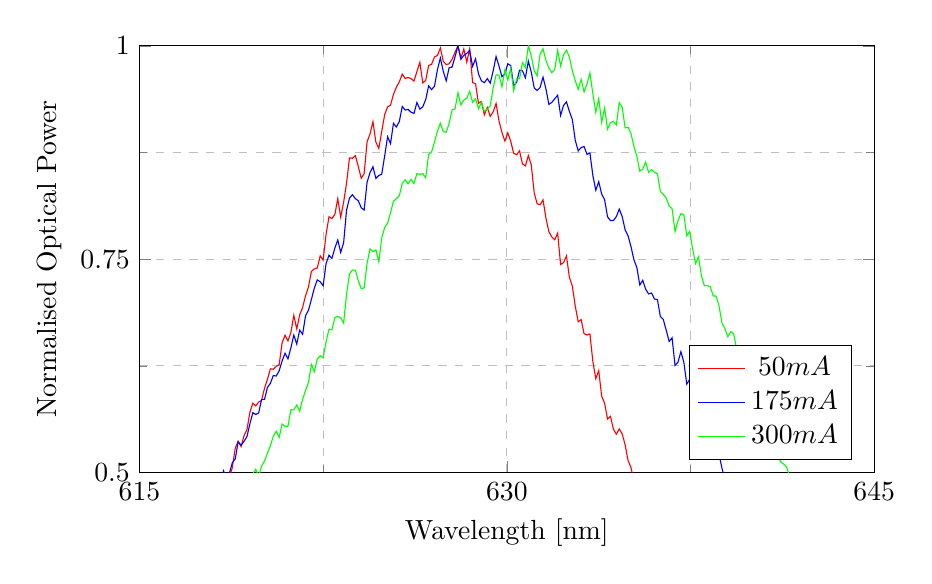
\begin{tikzpicture}

\begin{axis}[
    %title={Temperature dependence of CuSO$_4\cdot$5H$_2$O solubility},
    xlabel={Wavelength [nm]},
    ylabel={Normalised Optical Power},
    height=7cm,
    width=0.9\textwidth,
    xmin=615, xmax=645,
    ymin=0.5, ymax=1,
    % xtick={300, 450, 600, 750},
    % ytick={0.0, 0.25, 0.5, 0.75, 1.0},
    xtick={615, 630, 645},
    ytick={0.5, 0.75, 1.0},
    legend pos=south east,
    ymajorgrids=true,
    yminorgrids=true,
    xmajorgrids=true,
    xminorgrids=true,
    minor tick num=1,
    grid style=dashed,
]

\addplot[color=red]
  coordinates {
  (321.5116882,0.0006542079270406207)
  (321.6192017,0.0004690547159199363)
  (321.7267151,0.003653689484990084)
  (321.834259,0.0031722911874207307)
  (321.941803,-0.001086232000806948)
  (322.0493164,0.00024687091395480474)
  (322.1568909,-0.0007529562720283499)
  (322.2644348,9.874836429478485e-05)
  (322.3720093,0.0006171772848870119)
  (322.4795837,0.0031352605967526035)
  (322.5871582,0.0023205865705809717)
  (322.6947327,-0.0008640481473563349)
  (322.8023376,0.0015059125442330199)
  (322.9099426,0.0023946477519172257)
  (323.0175476,-0.00038264990127246285)
  (323.1251526,-0.0005678031122168271)
  (323.2327881,0.0018391882730116182)
  (323.3404236,0.0003949934571791394)
  (323.4480591,0.002913076846449274)
  (323.5556946,9.874836429478485e-05)
  (323.6633606,0.0006171772848870119)
  (323.7710266,-0.0015305996047372114)
  (323.8786926,0.00024687091395480474)
  (323.9863586,-4.9374182138576416e-05)
  (324.0940552,0.005505221493931245)
  (324.2017517,0.0004320240737663275)
  (324.3094482,0.0003949934571791394)
  (324.4171448,-0.001900905924712897)
  (324.5248718,0.0030982300060844767)
  (324.6325989,9.874836429478485e-05)
  (324.7403259,0.0009134223713356812)
  (324.848053,-0.001382477138564779)
  (324.9558105,0.0022835559799128445)
  (325.0635681,0.002098402820277642)
  (325.1713257,0.003394475144018628)
  (325.2790833,0.00154294323769579)
  (325.3868713,0.0023946477519172257)
  (325.4946594,-0.0006048337545467561)
  (325.6024475,0.001765127091675364)
  (325.7102356,-0.0005307724700632183)
  (325.8180542,0.0022835559799128445)
  (325.9258728,-0.001197323876134933)
  (326.0336914,0.0022465253892447177)
  (326.14151,0.00035796281484921043)
  (326.2493591,0.0020613720233149477)
  (326.3571777,0.0006912385691942295)
  (326.4650269,0.001617004522179328)
  (326.5729065,-0.0006418643967003649)
  (326.6807556,0.0011726368154544216)
  (326.7886353,-0.0005678031122168271)
  (326.8965149,0.0013577899752659443)
  (327.0043945,0.003394475144018628)
  (327.1123047,-0.0016416915826835193)
  (327.2202148,-0.0020860592888794654)
  (327.328125,0.0028390154588184527)
  (327.4360352,6.171772848870119e-05)
  (327.5439758,0.0018762188636797452)
  (327.651886,0.0010615449401264365)
  (327.7598267,0.0022835559799128445)
  (327.8677979,0.0015059125442330199)
  (327.9757385,0.002172464001613896)
  (328.0837097,0.0007282692115241584)
  (328.1916809,0.0007652998023686057)
  (328.2996521,0.0007282692115241584)
  (328.4076538,2.468709107810422e-05)
  (328.515625,0.0006912385691942295)
  (328.6236267,0.001024514246663666)
  (328.7316589,0.0002098402716248758)
  (328.8396606,0.0012837287934007297)
  (328.9476929,0.0009504529621801285)
  (329.0557251,0.00017280964230737336)
  (329.1637573,0.00017280964230737336)
  (329.2717896,0.002727923480519504)
  (329.3798523,-0.000975140125478963)
  (329.487915,0.0002098402716248758)
  (329.5959778,-0.0014195077294092264)
  (329.704071,-0.00012343545695977034)
  (329.8121338,-0.00038264990127246285)
  (329.9202271,0.0004320240737663275)
  (330.0283203,0.0006171772848870119)
  (330.1364441,0.000543116000403474)
  (330.2445374,2.468709107810422e-05)
  (330.3526611,0.0020613720233149477)
  (330.4607849,0.0009874836556428989)
  (330.5689392,-0.001049201409786181)
  (330.677063,-0.0006418643967003649)
  (330.7852173,-0.0003456192846852748)
  (330.8933716,0.0004690547159199363)
  (331.0015564,0.0016540351130237751)
  (331.1097107,-0.0006418643967003649)
  (331.2178955,-0.0006788949877211323)
  (331.3260803,0.002542770320884301)
  (331.4342651,0.003246352575051552)
  (331.5424805,2.468709107810422e-05)
  (331.6506958,-0.0007529562720283499)
  (331.7589111,-0.0007899869143582788)
  (331.8671265,-0.0012713851606184709)
  (331.9753723,-0.0007159256298747411)
  (332.0835876,9.874836429478485e-05)
  (332.1918335,0.0015059125442330199)
  (332.3001099,0.0009504529621801285)
  (332.4083557,-0.0023082430409459963)
  (332.5166321,-0.0007159256298747411)
  (332.6249084,-0.0015305996047372114)
  (332.7331848,-0.0004196805434260717)
  (332.8414612,0.0025798011178469957)
  (332.9497681,0.004579455283166097)
  (333.058075,0.0009874836556428989)
  (333.1663818,0.00017280964230737336)
  (333.2747192,-0.0011232626942697186)
  (333.3830261,-0.0004196805434260717)
  (333.4913635,0.000543116000403474)
  (333.5997009,0.0009874836556428989)
  (333.7080688,-0.0016787221737042867)
  (333.8164368,0.0012096675090935121)
  (333.9247742,-0.0012343545695977036)
  (334.0331726,0.0019873108419786937)
  (334.1415405,-0.0013454464449256887)
  (334.2499084,0.0006542079270406207)
  (334.3583069,9.874836429478485e-05)
  (334.4667053,0.00017280964230737336)
  (334.5751343,0.0010985755309708839)
  (334.6835327,0.0011726368154544216)
  (334.7919617,0.00024687091395480474)
  (334.9003906,0.0012837287934007297)
  (335.0088196,-0.000975140125478963)
  (335.1172791,0.0017280962948889897)
  (335.2257385,0.0004690547159199363)
  (335.334198,-0.0005307724700632183)
  (335.4426575,0.0008763917803149138)
  (335.5511169,0.0006912385691942295)
  (335.6596069,-0.0018268447433766428)
  (335.7680969,0.002172464001613896)
  (335.8765869,-0.0011232626942697186)
  (335.9851074,0.0013577899752659443)
  (336.0935974,-0.0010121707163234103)
  (336.2021179,0.0013577899752659443)
  (336.3106384,0.0008393610868521434)
  (336.4191895,0.0016540351130237751)
  (336.5277405,-0.0004196805434260717)
  (336.636261,-0.002271212448514668)
  (336.7448425,2.468709107810422e-05)
  (336.8533936,0.0022835559799128445)
  (336.9619446,0.006468018089069953)
  (337.0705261,0.00028390155610841353)
  (337.1791077,0.0007652998023686057)
  (337.2877197,-0.0011602932851141657)
  (337.3963013,-0.0009381094318398726)
  (337.5049133,0.0007652998023686057)
  (337.6135254,-0.0015305996047372114)
  (337.7221375,0.00154294323769579)
  (337.83078,0.001617004522179328)
  (337.9394226,9.874836429478485e-05)
  (338.0480652,-0.0012343545695977036)
  (338.1567078,0.0006542079270406207)
  (338.2653503,0.0002098402716248758)
  (338.3740234,-0.0008270175565118876)
  (338.4826965,-0.0005678031122168271)
  (338.5913696,-0.001049201409786181)
  (338.7000427,-0.0004937418279096095)
  (338.8087463,-8.640482115368668e-05)
  (338.91745,0.0018391882730116182)
  (339.0261536,0.0004690547159199363)
  (339.1348572,-0.0018268447433766428)
  (339.2435913,0.00024687091395480474)
  (339.3523254,-0.002345273631614124)
  (339.4610596,0.002357617161249099)
  (339.5697937,-0.0001974967285895697)
  (339.6785583,0.0022465253892447177)
  (339.787323,-0.0007159256298747411)
  (339.8960876,0.001765127091675364)
  (340.0048523,-4.9374182138576416e-05)
  (340.1136169,-0.0015305996047372114)
  (340.2224121,-0.0001974967285895697)
  (340.3312073,0.00361665868802739)
  (340.4400024,0.0026538622991832497)
  (340.5488281,6.171772848870119e-05)
  (340.6576233,0.0005801466425570829)
  (340.766449,0.002542770320884301)
  (340.8752747,-0.001086232000806948)
  (340.9841309,0.0006542079270406207)
  (341.0929565,-0.001197323876134933)
  (341.2018127,0.0019132496606424393)
  (341.3106689,0.0009874836556428989)
  (341.4195557,-0.00045671118557968053)
  (341.5284119,0.001765127091675364)
  (341.6372986,0.0025798011178469957)
  (341.7461853,-0.001086232000806948)
  (341.855072,-0.0007899869143582788)
  (341.9639893,-0.0017898141509453144)
  (342.0729065,0.0022835559799128445)
  (342.1818237,0.0005801466425570829)
  (342.290741,0.0012466980999379592)
  (342.3996582,0.0014688819532122524)
  (342.508606,0.0006542079270406207)
  (342.6175537,2.468709107810422e-05)
  (342.7265015,0.0012096675090935121)
  (342.8354492,0.0013577899752659443)
  (342.9444275,-0.0006048337545467561)
  (343.0534058,-0.0007529562720283499)
  (343.162384,0.003320413756387806)
  (343.2713623,0.0006912385691942295)
  (343.3803711,0.003024168618453655)
  (343.4893799,-0.00012343545695977034)
  (343.5983887,0.0002098402716248758)
  (343.7073975,-0.002271212448514668)
  (343.8164063,-0.0026044881771169464)
  (343.9254456,0.0005060853580735451)
  (344.0344849,0.0007282692115241584)
  (344.1435242,6.171772848870119e-05)
  (344.252594,0.0013948206689050348)
  (344.3616333,0.0001357790001008685)
  (344.4707031,-0.001197323876134933)
  (344.5798035,-0.0019379367199123898)
  (344.6888733,-0.0008640481473563349)
  (344.7979736,-0.0017898141509453144)
  (344.9070435,0.0018391882730116182)
  (345.0161438,-0.0016416915826835193)
  (345.1252747,0.0023205865705809717)
  (345.234375,0.0008023304445222145)
  (345.3435059,0.0015799738285402374)
  (345.4526367,0.0008393610868521434)
  (345.5617676,-0.0008640481473563349)
  (345.670929,0.0024316785488799203)
  (345.7800598,-0.0023082430409459963)
  (345.8892212,-0.001197323876134933)
  (345.9984131,0.0008393610868521434)
  (346.1075745,0.001024514246663666)
  (346.2167664,-0.0016416915826835193)
  (346.3259277,0.0018762188636797452)
  (346.4351501,0.0018391882730116182)
  (346.544342,2.468709107810422e-05)
  (346.6535339,0.00154294323769579)
  (346.7627563,0.00028390155610841353)
  (346.8719788,-0.001382477138564779)
  (346.9812317,-0.0009381094318398726)
  (347.0904541,-4.9374182138576416e-05)
  (347.199707,-0.001604660889220749)
  (347.30896,0.005097884377698145)
  (347.4182129,-0.0007899869143582788)
  (347.5274658,0.00024687091395480474)
  (347.6367493,0.0005801466425570829)
  (347.7460327,0.0018391882730116182)
  (347.8553162,0.0018762188636797452)
  (347.9645996,0.0009504529621801285)
  (348.0739136,0.0019132496606424393)
  (348.1832275,0.0009874836556428989)
  (348.2925415,0.0008763917803149138)
  (348.4018555,0.0022835559799128445)
  (348.5112,0.0017280962948889897)
  (348.6205139,0.003246352575051552)
  (348.7298584,0.0012466980999379592)
  (348.8392029,0.002542770320884301)
  (348.9485779,9.874836429478485e-05)
  (349.0579529,0.0014318512597494822)
  (349.1672974,-0.0003456192846852748)
  (349.2767029,-0.0007899869143582788)
  (349.3860779,-0.0008270175565118876)
  (349.4954834,-0.000271558000201737)
  (349.6048584,0.0019873108419786937)
  (349.7142639,0.0007282692115241584)
  (349.8237,0.0033574443470559333)
  (349.9331055,-0.000271558000201737)
  (350.0425415,0.00028390155610841353)
  (350.1519775,0.0014688819532122524)
  (350.2614136,0.0004320240737663275)
  (350.3708496,0.0007282692115241584)
  (350.4803162,0.0013577899752659443)
  (350.5897827,0.0009134223713356812)
  (350.6992493,0.0003209321984383425)
  (350.8087158,-0.0003085886423553459)
  (350.9182129,-0.00038264990127246285)
  (351.02771,-0.00045671118557968053)
  (351.137207,-0.0006048337545467561)
  (351.2467041,-0.00038264990127246285)
  (351.3562317,0.0013948206689050348)
  (351.4657288,0.001802157682343491)
  (351.5752563,0.00017280964230737336)
  (351.6847839,0.005283037537333348)
  (351.794342,0.0007652998023686057)
  (351.9038696,0.0004320240737663275)
  (352.0134277,0.0003949934571791394)
  (352.1229858,-0.0008640481473563349)
  (352.2325745,0.0018762188636797452)
  (352.3421326,0.002357617161249099)
  (352.4517212,6.171772848870119e-05)
  (352.5613098,0.0012837287934007297)
  (352.6708984,0.003394475144018628)
  (352.7805176,0.0009134223713356812)
  (352.8901062,0.0007652998023686057)
  (352.9997253,-0.0012713851606184709)
  (353.1093445,0.0020243414326468205)
  (353.2189941,0.0013577899752659443)
  (353.3286133,-0.00045671118557968053)
  (353.4382629,-0.00016046609918390724)
  (353.5479126,-0.00016046609918390724)
  (353.6575928,0.0030611992091217825)
  (353.7672424,0.0015059125442330199)
  (353.8769226,0.0022094945922820236)
  (353.9866028,-0.0021230898795475926)
  (354.096283,0.002172464001613896)
  (354.2059631,-0.0011232626942697186)
  (354.3156738,0.0006912385691942295)
  (354.4253845,0.0006171772848870119)
  (354.5350952,0.0013577899752659443)
  (354.6448059,-0.0017157528671670572)
  (354.7545471,0.0009874836556428989)
  (354.8642883,0.0003949934571791394)
  (354.9740295,0.0012096675090935121)
  (355.0837708,-0.00045671118557968053)
  (355.193512,0.0015799738285402374)
  (355.3032837,6.171772848870119e-05)
  (355.4130554,0.0024316785488799203)
  (355.5228271,0.0016540351130237751)
  (355.6325989,0.0013207593844214971)
  (355.7424011,-0.001049201409786181)
  (355.8522034,-0.00038264990127246285)
  (355.9620056,0.002098402820277642)
  (356.0718079,0.0002098402716248758)
  (356.1816406,0.0020613720233149477)
  (356.2914429,-4.9374182138576416e-05)
  (356.4012756,0.0004690547159199363)
  (356.5111084,0.00024687091395480474)
  (356.6209717,0.0028390154588184527)
  (356.730835,0.004801639239763994)
  (356.8406677,0.0016540351130237751)
  (356.950531,0.002135433410945769)
  (357.0604248,0.0006912385691942295)
  (357.1702881,0.0014688819532122524)
  (357.2801819,0.00028390155610841353)
  (357.3900757,0.0016910657038682224)
  (357.4999695,0.0005801466425570829)
  (357.6098938,-0.0003085886423553459)
  (357.7197876,0.0006542079270406207)
  (357.8297119,0.0016910657038682224)
  (357.9396362,0.000543116000403474)
  (358.0495911,0.0018762188636797452)
  (358.1595154,0.0005801466425570829)
  (358.2694702,-0.0008640481473563349)
  (358.379425,-0.001900905924712897)
  (358.4893799,0.0008763917803149138)
  (358.5993652,-4.9374182138576416e-05)
  (358.7093201,0.0023205865705809717)
  (358.8193054,0.0025798011178469957)
  (358.9292908,0.0002098402716248758)
  (359.0393066,0.00017280964230737336)
  (359.149292,0.0027649542774821983)
  (359.2593079,9.874836429478485e-05)
  (359.3693237,-0.0007529562720283499)
  (359.4793396,-0.002160120471978921)
  (359.589386,0.00035796281484921043)
  (359.6994019,-0.0014195077294092264)
  (359.8094482,-0.000271558000201737)
  (359.9194946,0.003024168618453655)
  (360.0295715,0.0009504529621801285)
  (360.1396179,-0.0017157528671670572)
  (360.2496948,0.0008393610868521434)
  (360.3597717,-4.9374182138576416e-05)
  (360.4698486,0.0009134223713356812)
  (360.5799561,0.0009134223713356812)
  (360.690033,-0.00012343545695977034)
  (360.8001404,-0.0014195077294092264)
  (360.9102478,0.0004690547159199363)
  (361.0203857,0.0014688819532122524)
  (361.1304932,0.0011726368154544216)
  (361.2406311,0.0006542079270406207)
  (361.350769,0.0024316785488799203)
  (361.460907,-0.0001974967285895697)
  (361.5710754,0.00035796281484921043)
  (361.6812439,-0.00016046609918390724)
  (361.7914124,-0.0016787221737042867)
  (361.9015808,0.0009874836556428989)
  (362.0117493,0.0033574443470559333)
  (362.1219482,0.0005060853580735451)
  (362.2321167,0.005468190696968551)
  (362.3423157,-0.0009381094318398726)
  (362.4525452,-0.0011602932851141657)
  (362.5627441,-0.0008270175565118876)
  (362.6729736,0.003468536325354882)
  (362.7832031,-1.2343545535525704e-05)
  (362.8934326,-0.00038264990127246285)
  (363.0036621,-0.00038264990127246285)
  (363.1139221,-0.0004196805434260717)
  (363.2241821,-0.0004937418279096095)
  (363.3344421,0.0005060853580735451)
  (363.4447021,-0.0004937418279096095)
  (363.5549622,0.0025798011178469957)
  (363.6652527,0.00028390155610841353)
  (363.7755432,0.003024168618453655)
  (363.8858337,0.0016910657038682224)
  (363.9961243,0.0025057397302161743)
  (364.1064453,0.0010615449401264365)
  (364.2167664,0.001024514246663666)
  (364.3270874,0.00024687091395480474)
  (364.4374084,-0.0009381094318398726)
  (364.5477295,0.0009504529621801285)
  (364.6580811,0.0009134223713356812)
  (364.7684326,-0.0017157528671670572)
  (364.8787842,0.0016910657038682224)
  (364.9891357,-0.000975140125478963)
  (365.0995178,0.0006542079270406207)
  (365.2098999,-0.0017527835608061478)
  (365.320282,0.001024514246663666)
  (365.4306641,-0.0008270175565118876)
  (365.5410461,0.0003949934571791394)
  (365.6514587,-0.001493569013892764)
  (365.7618713,0.001802157682343491)
  (365.8722839,-0.0004937418279096095)
  (365.9826965,-0.0011232626942697186)
  (366.0931396,0.0005801466425570829)
  (366.2035522,0.003653689484990084)
  (366.3139954,6.171772848870119e-05)
  (366.4244385,0.0003209321984383425)
  (366.5349121,0.0006171772848870119)
  (366.6453552,-0.00016046609918390724)
  (366.7558289,0.0010985755309708839)
  (366.8663025,0.0022465253892447177)
  (366.9768066,-0.0009010788409954254)
  (367.0872803,0.0007282692115241584)
  (367.1977844,-0.0012343545695977036)
  (367.3082886,-0.0009381094318398726)
  (367.4187927,0.0006912385691942295)
  (367.5292969,0.002172464001613896)
  (367.6398315,-0.00038264990127246285)
  (367.7503662,0.00017280964230737336)
  (367.8609009,0.0032833831657196793)
  (367.9714355,-0.001049201409786181)
  (368.0819702,-0.0009010788409954254)
  (368.1925354,0.0012466980999379592)
  (368.3031006,-0.0004196805434260717)
  (368.4136658,-0.0012343545695977036)
  (368.524231,-0.001049201409786181)
  (368.6348267,-0.00016046609918390724)
  (368.7453918,0.00035796281484921043)
  (368.8559875,0.001024514246663666)
  (368.9666138,0.0015799738285402374)
  (369.0772095,0.00028390155610841353)
  (369.1878357,0.0002098402716248758)
  (369.2984619,-8.640482115368668e-05)
  (369.4090881,-0.0002345273580481282)
  (369.5197144,0.0005801466425570829)
  (369.6303406,-0.0011232626942697186)
  (369.7409973,0.0022094945922820236)
  (369.8516541,0.0006542079270406207)
  (369.9623108,-0.0009381094318398726)
  (370.0729675,-0.0003085886423553459)
  (370.1836548,0.000543116000403474)
  (370.294342,-0.0016416915826835193)
  (370.4050293,0.001765127091675364)
  (370.5157166,0.0015799738285402374)
  (370.6264038,0.0006542079270406207)
  (370.7371216,0.0002098402716248758)
  (370.8478394,0.0019873108419786937)
  (370.9585571,-0.0017157528671670572)
  (371.0692749,0.0023205865705809717)
  (371.1800232,-1.2343545535525704e-05)
  (371.2907715,0.0005060853580735451)
  (371.4015198,0.0014688819532122524)
  (371.5122681,-8.640482115368668e-05)
  (371.6230164,0.0013577899752659443)
  (371.7337952,0.0028760460494865795)
  (371.8445435,0.00017280964230737336)
  (371.9553223,9.874836429478485e-05)
  (372.0661316,6.171772848870119e-05)
  (372.1769104,0.002542770320884301)
  (372.2877197,-0.001086232000806948)
  (372.3985291,-0.0004937418279096095)
  (372.5093384,0.0028760460494865795)
  (372.6201477,0.0022835559799128445)
  (372.7309875,0.001617004522179328)
  (372.8417969,0.0008023304445222145)
  (372.9526367,-0.0020119979030118456)
  (373.0635071,0.0028390154588184527)
  (373.1743469,0.0009504529621801285)
  (373.2852173,0.001024514246663666)
  (373.3960571,0.0010615449401264365)
  (373.5069275,0.0010615449401264365)
  (373.6178284,0.00028390155610841353)
  (373.7286987,0.0012466980999379592)
  (373.8395996,-0.0009010788409954254)
  (373.9505005,0.003394475144018628)
  (374.0614014,-0.0002345273580481282)
  (374.1723022,0.0017280962948889897)
  (374.2832336,-0.0037894685243221845)
  (374.3941345,-0.00012343545695977034)
  (374.5050659,0.0011726368154544216)
  (374.6159973,-0.0011232626942697186)
  (374.7269592,0.002135433410945769)
  (374.8378906,-0.0004196805434260717)
  (374.9488525,0.00017280964230737336)
  (375.0598145,-0.00038264990127246285)
  (375.1707764,0.0015799738285402374)
  (375.2817688,-0.0009010788409954254)
  (375.3927612,6.171772848870119e-05)
  (375.5037231,0.0012837287934007297)
  (375.6147156,0.0022465253892447177)
  (375.7257385,0.00035796281484921043)
  (375.836731,6.171772848870119e-05)
  (375.9477539,0.004653516877091485)
  (376.0587769,-0.0007529562720283499)
  (376.1697998,0.0016540351130237751)
  (376.2808228,0.0005801466425570829)
  (376.3918762,0.0009504529621801285)
  (376.5029297,0.0004320240737663275)
  (376.6139832,-0.0006418643967003649)
  (376.7250366,-0.0006048337545467561)
  (376.8360901,0.0016910657038682224)
  (376.9471741,-0.002530426791249326)
  (377.0582581,0.0007652998023686057)
  (377.169342,0.0022835559799128445)
  (377.280426,0.00028390155610841353)
  (377.3915405,-0.0018268447433766428)
  (377.5026245,0.000543116000403474)
  (377.613739,-0.000975140125478963)
  (377.7248535,0.0012837287934007297)
  (377.8359985,-0.00012343545695977034)
  (377.947113,0.002357617161249099)
  (378.0582581,0.0008393610868521434)
  (378.1694031,0.0011726368154544216)
  (378.2805481,-0.0005678031122168271)
  (378.3916931,0.0020613720233149477)
  (378.5028687,0.0006171772848870119)
  (378.6140442,0.0004690547159199363)
  (378.7252197,0.0008023304445222145)
  (378.8363953,0.0014318512597494822)
  (378.9475708,-0.001604660889220749)
  (379.0587769,0.002727923480519504)
  (379.1699829,-1.2343545535525704e-05)
  (379.281189,0.0019132496606424393)
  (379.392395,0.001024514246663666)
  (379.5036316,-0.0013084158540812413)
  (379.6148376,-0.0004196805434260717)
  (379.7260742,-0.00012343545695977034)
  (379.8373108,-0.0008270175565118876)
  (379.9485779,0.0015059125442330199)
  (380.0598145,-0.0003085886423553459)
  (380.1710815,0.0011726368154544216)
  (380.2823486,-0.0004937418279096095)
  (380.3936157,0.0009874836556428989)
  (380.5048828,0.00017280964230737336)
  (380.6161804,0.002987138027785528)
  (380.727478,0.0013948206689050348)
  (380.8387756,0.0009134223713356812)
  (380.9500732,0.0005801466425570829)
  (381.0613708,0.0012837287934007297)
  (381.172699,0.001617004522179328)
  (381.2840271,-0.0003085886423553459)
  (381.3953552,9.874836429478485e-05)
  (381.5066833,-0.0004196805434260717)
  (381.618042,0.002616831708515123)
  (381.7293701,0.0012096675090935121)
  (381.8407288,0.0006912385691942295)
  (381.9520874,0.0014318512597494822)
  (382.0634766,0.0017280962948889897)
  (382.1748352,0.0014318512597494822)
  (382.2862244,0.0013948206689050348)
  (382.3976135,0.003764781463289033)
  (382.5090027,0.0009874836556428989)
  (382.6203918,0.004394302123530895)
  (382.7318115,0.0016540351130237751)
  (382.8432007,0.003727750666326339)
  (382.9546204,0.00035796281484921043)
  (383.0660706,0.0012466980999379592)
  (383.1774902,0.0017280962948889897)
  (383.2889099,0.0024316785488799203)
  (383.4003601,0.0015799738285402374)
  (383.5118103,0.002542770320884301)
  (383.6232605,0.0008023304445222145)
  (383.7347412,-0.0002345273580481282)
  (383.8461914,0.0007652998023686057)
  (383.9576721,0.0005801466425570829)
  (384.0691528,-0.001604660889220749)
  (384.1806641,0.0015059125442330199)
  (384.2921448,-0.0013084158540812413)
  (384.403656,0.0016910657038682224)
  (384.5151672,-0.0002345273580481282)
  (384.6266785,-0.0017898141509453144)
  (384.7381897,-0.002826671929183477)
  (384.8497009,0.0012096675090935121)
  (384.9612427,-0.0014195077294092264)
  (385.0727844,0.0008023304445222145)
  (385.1843262,-0.000271558000201737)
  (385.2958679,0.0011356062246099742)
  (385.4074402,0.0008393610868521434)
  (385.5190125,0.002357617161249099)
  (385.6305542,-0.0026415187695482747)
  (385.742157,0.0028760460494865795)
  (385.8537292,-0.0023082430409459963)
  (385.9653015,-0.0010121707163234103)
  (386.0769043,0.0014318512597494822)
  (386.1885071,0.0025057397302161743)
  (386.3001099,0.0003949934571791394)
  (386.4117432,-0.00045671118557968053)
  (386.5233459,-0.00012343545695977034)
  (386.6349792,-8.640482115368668e-05)
  (386.7466125,0.0016910657038682224)
  (386.8582458,0.0009134223713356812)
  (386.9699097,-0.000271558000201737)
  (387.081543,0.0018762188636797452)
  (387.1932068,0.0010615449401264365)
  (387.3048706,-0.0013084158540812413)
  (387.4165344,-0.0001974967285895697)
  (387.5282288,-0.000975140125478963)
  (387.6398926,9.874836429478485e-05)
  (387.7515869,0.001765127091675364)
  (387.8632813,0.0004690547159199363)
  (387.9749756,0.0011356062246099742)
  (388.0867004,0.0008393610868521434)
  (388.1983948,9.874836429478485e-05)
  (388.3101196,-0.0013084158540812413)
  (388.4218445,0.0009874836556428989)
  (388.5335693,-0.0009381094318398726)
  (388.6453247,0.0006912385691942295)
  (388.7570801,-0.000271558000201737)
  (388.8688049,-0.0007899869143582788)
  (388.9805603,0.0011726368154544216)
  (389.0923462,0.000543116000403474)
  (389.2041016,0.0014318512597494822)
  (389.3158875,0.0006171772848870119)
  (389.4276733,0.001765127091675364)
  (389.5394592,0.0023946477519172257)
  (389.6512451,0.00028390155610841353)
  (389.7630615,-0.0004937418279096095)
  (389.8748474,-0.0006418643967003649)
  (389.9866638,0.0004690547159199363)
  (390.0984802,-0.001382477138564779)
  (390.2103271,0.004135087782559438)
  (390.3221436,0.0004690547159199363)
  (390.4339905,0.001802157682343491)
  (390.5458374,0.001024514246663666)
  (390.6576843,0.0031722911874207307)
  (390.7695313,-0.0011602932851141657)
  (390.8814087,-0.0013454464449256887)
  (390.9932556,-0.0015676302983763017)
  (391.1051331,0.0019132496606424393)
  (391.2170105,0.0016540351130237751)
  (391.3289185,0.0009874836556428989)
  (391.4407959,0.0006542079270406207)
  (391.5527039,0.0008023304445222145)
  (391.6646118,-0.0011602932851141657)
  (391.7765198,0.0017280962948889897)
  (391.8884277,0.0008393610868521434)
  (392.0003662,0.0003949934571791394)
  (392.1123047,0.0018391882730116182)
  (392.2242432,0.0013577899752659443)
  (392.3361816,0.000543116000403474)
  (392.4481201,-0.0015305996047372114)
  (392.5600891,0.0004690547159199363)
  (392.6720276,0.003320413756387806)
  (392.7839966,-0.0001974967285895697)
  (392.8959961,0.002172464001613896)
  (393.0079651,0.0009504529621801285)
  (393.1199341,0.003690720281952779)
  (393.2319336,-0.0007159256298747411)
  (393.3439331,0.0004690547159199363)
  (393.4559326,-0.000271558000201737)
  (393.5679626,0.00024687091395480474)
  (393.6799622,0.0025057397302161743)
  (393.7919922,0.003912903825961541)
  (393.9040222,-1.2343545535525704e-05)
  (394.0160522,0.003690720281952779)
  (394.1280823,0.000543116000403474)
  (394.2401428,0.0006542079270406207)
  (394.3522034,0.003468536325354882)
  (394.4642639,0.004468363306630351)
  (394.5763245,-0.0005678031122168271)
  (394.688385,-0.0018268447433766428)
  (394.8004761,0.0025798011178469957)
  (394.9125671,0.0011726368154544216)
  (395.0246277,0.0012096675090935121)
  (395.1367493,0.0006912385691942295)
  (395.2488403,0.0018391882730116182)
  (395.3609619,0.0012837287934007297)
  (395.473053,0.00035796281484921043)
  (395.5851746,-4.9374182138576416e-05)
  (395.6972961,-0.0008640481473563349)
  (395.8094482,0.001617004522179328)
  (395.9215698,6.171772848870119e-05)
  (396.0337219,0.0009134223713356812)
  (396.145874,0.0006912385691942295)
  (396.2580261,0.0016910657038682224)
  (396.3702087,0.000543116000403474)
  (396.4823608,-0.00038264990127246285)
  (396.5945435,0.002542770320884301)
  (396.7067261,0.002135433410945769)
  (396.8189087,0.00024687091395480474)
  (396.9310913,0.0011356062246099742)
  (397.0433044,-0.0005678031122168271)
  (397.1555176,0.0023205865705809717)
  (397.2677002,0.0006542079270406207)
  (397.3799438,0.0009504529621801285)
  (397.492157,-0.0010121707163234103)
  (397.6043701,-0.0015305996047372114)
  (397.7166138,0.0009874836556428989)
  (397.8288574,0.0018762188636797452)
  (397.9411011,0.0013207593844214971)
  (398.0533752,0.0007652998023686057)
  (398.1656189,0.0018391882730116182)
  (398.2778931,0.0028760460494865795)
  (398.3901672,0.001617004522179328)
  (398.5024414,0.0023205865705809717)
  (398.6147156,-0.001900905924712897)
  (398.7270203,-0.0005307724700632183)
  (398.8392944,0.0009134223713356812)
  (398.9515991,0.0016910657038682224)
  (399.0639038,-0.0013084158540812413)
  (399.176239,9.874836429478485e-05)
  (399.2885437,-0.00045671118557968053)
  (399.4008789,0.004801639239763994)
  (399.5132141,0.0009134223713356812)
  (399.6255493,0.0006912385691942295)
  (399.7378845,-0.0001974967285895697)
  (399.8502502,-0.00045671118557968053)
  (399.9625854,0.0006912385691942295)
  (400.0749512,0.002357617161249099)
  (400.1873169,0.0019502802513105667)
  (400.2996826,0.0006542079270406207)
  (400.4120789,0.0020613720233149477)
  (400.5244446,0.001024514246663666)
  (400.6368408,0.0007652998023686057)
  (400.7492371,-0.0020490284936799724)
  (400.8616638,0.0019502802513105667)
  (400.9740601,-0.000975140125478963)
  (401.0864868,0.00024687091395480474)
  (401.1989136,-0.001382477138564779)
  (401.3113403,-0.0007159256298747411)
  (401.4237671,-8.640482115368668e-05)
  (401.5361938,0.0026908928898513773)
  (401.6486511,-0.0011602932851141657)
  (401.7611084,-0.0019749673105805172)
  (401.8735657,0.0013948206689050348)
  (401.9860229,-0.0004196805434260717)
  (402.0984802,-0.00038264990127246285)
  (402.210968,0.0010615449401264365)
  (402.3234558,0.0008023304445222145)
  (402.4359436,0.0017280962948889897)
  (402.5484314,-0.0007529562720283499)
  (402.6609192,0.000543116000403474)
  (402.7734375,-0.0015305996047372114)
  (402.8859253,-0.00045671118557968053)
  (402.9984436,-0.0009381094318398726)
  (403.1109619,-0.0023082430409459963)
  (403.2235107,0.0007282692115241584)
  (403.3360291,-0.0005678031122168271)
  (403.4485779,0.001765127091675364)
  (403.5611267,-0.0016787221737042867)
  (403.6736755,-0.0003456192846852748)
  (403.7862244,-0.0005678031122168271)
  (403.8988037,0.0016540351130237751)
  (404.0113831,-0.0026785493602164015)
  (404.1239319,-1.2343545535525704e-05)
  (404.2365417,-0.0006048337545467561)
  (404.3491211,0.00028390155610841353)
  (404.4617004,-0.001493569013892764)
  (404.5743103,-0.003715407341222729)
  (404.6869202,0.001617004522179328)
  (404.79953,-0.0003456192846852748)
  (404.9121399,-0.0013454464449256887)
  (405.0247803,0.0030982300060844767)
  (405.1373901,-1.2343545535525704e-05)
  (405.2500305,0.0006542079270406207)
  (405.3626709,0.0012096675090935121)
  (405.4753113,0.0015059125442330199)
  (405.5879822,0.0015799738285402374)
  (405.7006226,-0.0007529562720283499)
  (405.8132935,0.0026538622991832497)
  (405.9259644,0.0015799738285402374)
  (406.0386353,6.171772848870119e-05)
  (406.1513062,0.002357617161249099)
  (406.2640076,0.0005801466425570829)
  (406.376709,0.0013948206689050348)
  (406.4894104,6.171772848870119e-05)
  (406.6021118,0.002135433410945769)
  (406.7148132,0.0002098402716248758)
  (406.8275452,0.0028019848681503255)
  (406.9402466,-0.0013084158540812413)
  (407.0529785,0.0003209321984383425)
  (407.1657104,-0.0005307724700632183)
  (407.2784729,0.0004690547159199363)
  (407.3912048,-0.0027526107460840218)
  (407.5039673,-0.0002345273580481282)
  (407.6167297,-8.640482115368668e-05)
  (407.7294922,0.0012096675090935121)
  (407.8422546,-0.00045671118557968053)
  (407.9550171,-1.2343545535525704e-05)
  (408.0678101,0.0033574443470559333)
  (408.180603,0.0014318512597494822)
  (408.293396,-0.001382477138564779)
  (408.406189,0.00028390155610841353)
  (408.5189819,-0.0014195077294092264)
  (408.6318054,-0.00045671118557968053)
  (408.7446289,0.003209321778088858)
  (408.8574524,0.0010615449401264365)
  (408.9702759,-0.0010121707163234103)
  (409.0830994,0.0014688819532122524)
  (409.1959534,-0.0018268447433766428)
  (409.3087769,-0.0024193350174817434)
  (409.4216309,0.0009134223713356812)
  (409.5344849,-0.0017157528671670572)
  (409.6473694,-0.0020860592888794654)
  (409.7602234,0.0007652998023686057)
  (409.8731079,0.0031722911874207307)
  (409.9859924,0.0003949934571791394)
  (410.098877,0.001024514246663666)
  (410.2117615,-0.0013084158540812413)
  (410.324646,-0.0019749673105805172)
  (410.437561,-0.0008270175565118876)
  (410.5504761,0.0011356062246099742)
  (410.6633911,-0.0017527835608061478)
  (410.7763062,0.0008763917803149138)
  (410.8892212,-0.00038264990127246285)
  (411.0021667,-0.0028637025198516046)
  (411.1151123,0.0022835559799128445)
  (411.2280579,-0.003604315364686982)
  (411.3410034,-0.0012343545695977036)
  (411.453949,9.874836429478485e-05)
  (411.566925,-0.0017157528671670572)
  (411.6798706,0.004616486080128791)
  (411.7928467,0.0017280962948889897)
  (411.9058228,-0.001086232000806948)
  (412.0187988,0.0009504529621801285)
  (412.1318054,-0.0011232626942697186)
  (412.2447815,-0.0012713851606184709)
  (412.3577881,0.0023946477519172257)
  (412.4707947,0.0020243414326468205)
  (412.5838318,-0.00012343545695977034)
  (412.6968384,-0.0006418643967003649)
  (412.8098755,-0.0013454464449256887)
  (412.9228821,0.0018391882730116182)
  (413.0359192,0.0010985755309708839)
  (413.1489563,0.004246179760858387)
  (413.2620239,0.0016910657038682224)
  (413.375061,0.0002098402716248758)
  (413.4881287,-0.005011479460432349)
  (413.6011963,0.004209148963895693)
  (413.7142639,0.0014318512597494822)
  (413.8273315,0.0023946477519172257)
  (413.9404297,-0.0006788949877211323)
  (414.0534973,0.0008763917803149138)
  (414.1665955,2.468709107810422e-05)
  (414.2796936,0.0002098402716248758)
  (414.3927917,0.0015059125442330199)
  (414.5059204,-0.0017527835608061478)
  (414.6190186,0.0006171772848870119)
  (414.7321472,-0.0017898141509453144)
  (414.8452759,-0.000975140125478963)
  (414.9584045,0.0007652998023686057)
  (415.0715332,-0.0007899869143582788)
  (415.1846924,-0.0007159256298747411)
  (415.2978516,9.874836429478485e-05)
  (415.4109802,-0.0002345273580481282)
  (415.5241699,0.0012096675090935121)
  (415.6373291,0.0026538622991832497)
  (415.7504883,0.0011356062246099742)
  (415.863678,0.0004690547159199363)
  (415.9768677,-0.0033451008174209583)
  (416.0900574,-0.0002345273580481282)
  (416.2032471,0.0009134223713356812)
  (416.3164368,0.00028390155610841353)
  (416.429657,0.0016540351130237751)
  (416.5428467,0.0009504529621801285)
  (416.6560669,-0.0018268447433766428)
  (416.7693176,-0.00012343545695977034)
  (416.8825378,-0.0005678031122168271)
  (416.9957581,0.004986792399399197)
  (417.1090088,-0.0003456192846852748)
  (417.2222595,-0.00016046609918390724)
  (417.3355103,0.0011726368154544216)
  (417.448761,0.0004320240737663275)
  (417.5620117,-0.0015305996047372114)
  (417.675293,0.002727923480519504)
  (417.7885742,0.001024514246663666)
  (417.9018555,-0.00016046609918390724)
  (418.0151367,0.002135433410945769)
  (418.128418,0.0011356062246099742)
  (418.2417297,0.0026538622991832497)
  (418.355011,-0.00012343545695977034)
  (418.4683228,0.0008393610868521434)
  (418.5816345,0.0012466980999379592)
  (418.6949768,-0.0016787221737042867)
  (418.8082886,0.0015059125442330199)
  (418.9216309,-0.0020119979030118456)
  (419.0349426,0.0015059125442330199)
  (419.1482849,0.0011356062246099742)
  (419.2616577,0.002616831708515123)
  (419.375,-0.0024933962005811994)
  (419.4883423,0.0014318512597494822)
  (419.6017151,-0.0022341816533151754)
  (419.7150879,0.0006912385691942295)
  (419.8284607,-0.0006048337545467561)
  (419.9418335,0.0010985755309708839)
  (420.0552368,0.0013577899752659443)
  (420.1686401,0.0009134223713356812)
  (420.2820129,0.00154294323769579)
  (420.3954163,0.0013207593844214971)
  (420.5088501,-0.0002345273580481282)
  (420.6222534,0.0005060853580735451)
  (420.7356567,-0.00038264990127246285)
  (420.8490906,0.0007652998023686057)
  (420.9625244,-0.0008270175565118876)
  (421.0759583,-8.640482115368668e-05)
  (421.1893921,0.001765127091675364)
  (421.3028564,0.0015059125442330199)
  (421.4163208,-0.0019749673105805172)
  (421.5297546,-0.0009010788409954254)
  (421.643219,-0.0011232626942697186)
  (421.7567139,0.0011356062246099742)
  (421.8701782,-0.0006418643967003649)
  (421.9836426,0.0018762188636797452)
  (422.0971375,-0.002826671929183477)
  (422.2106323,0.0007652998023686057)
  (422.3241272,9.874836429478485e-05)
  (422.4376526,-0.00012343545695977034)
  (422.5511475,-0.0008640481473563349)
  (422.6646729,0.002172464001613896)
  (422.7781677,0.00154294323769579)
  (422.8916931,0.003394475144018628)
  (423.005249,-0.001382477138564779)
  (423.1187744,0.003024168618453655)
  (423.2323303,-0.0017527835608061478)
  (423.3458557,0.00024687091395480474)
  (423.4594116,0.002135433410945769)
  (423.5729675,0.0018391882730116182)
  (423.686554,0.0015059125442330199)
  (423.8001099,0.00024687091395480474)
  (423.9136963,0.0018762188636797452)
  (424.0272522,-0.002530426791249326)
  (424.1408386,2.468709107810422e-05)
  (424.2544556,0.003320413756387806)
  (424.368042,-0.0021230898795475926)
  (424.4816589,-0.0008270175565118876)
  (424.5952454,0.0007652998023686057)
  (424.7088623,0.0018762188636797452)
  (424.8224792,0.0004320240737663275)
  (424.9360962,0.0011726368154544216)
  (425.0497437,0.00035796281484921043)
  (425.1633606,0.0013207593844214971)
  (425.2770081,-0.005307724598366499)
  (425.3906555,9.874836429478485e-05)
  (425.504303,-0.00038264990127246285)
  (425.617981,-0.0006788949877211323)
  (425.7316284,0.00154294323769579)
  (425.8453064,0.000543116000403474)
  (425.9589844,-0.0001974967285895697)
  (426.0726624,0.0026538622991832497)
  (426.1863403,-0.0004937418279096095)
  (426.3000488,0.004394302123530895)
  (426.4137268,0.0002098402716248758)
  (426.5274353,-4.9374182138576416e-05)
  (426.6411438,0.0002098402716248758)
  (426.7548523,-0.0003085886423553459)
  (426.8685608,-0.0003456192846852748)
  (426.9822998,0.0015799738285402374)
  (427.0960083,-0.0005678031122168271)
  (427.2097473,-0.0005307724700632183)
  (427.3234863,0.0018391882730116182)
  (427.4372253,0.0008023304445222145)
  (427.5509949,-0.0023082430409459963)
  (427.6647339,0.0017280962948889897)
  (427.7785034,0.0006542079270406207)
  (427.8922729,0.0022835559799128445)
  (428.0060425,-0.0012713851606184709)
  (428.119812,0.0015799738285402374)
  (428.2336121,-0.0009010788409954254)
  (428.3473816,0.002098402820277642)
  (428.4611816,-0.00016046609918390724)
  (428.5749817,0.0010985755309708839)
  (428.6887817,-0.0003456192846852748)
  (428.8026123,-1.2343545535525704e-05)
  (428.9164124,0.0003949934571791394)
  (429.0302429,0.0017280962948889897)
  (429.1440735,-0.001049201409786181)
  (429.2579041,0.001024514246663666)
  (429.3717346,-0.001382477138564779)
  (429.4855652,0.0014318512597494822)
  (429.5994263,-0.0003085886423553459)
  (429.7132874,0.0010615449401264365)
  (429.8271484,0.0007652998023686057)
  (429.9410095,-0.001382477138564779)
  (430.0548706,0.0012466980999379592)
  (430.1687317,0.0032833831657196793)
  (430.2826233,-0.0004196805434260717)
  (430.3965149,0.0008023304445222145)
  (430.5104065,0.0007282692115241584)
  (430.6242981,0.001024514246663666)
  (430.7381897,-0.0011602932851141657)
  (430.8521118,-0.0012713851606184709)
  (430.9660034,0.000543116000403474)
  (431.0799255,0.0012837287934007297)
  (431.1938477,-0.000271558000201737)
  (431.3078003,0.002616831708515123)
  (431.4217224,-0.0007529562720283499)
  (431.535675,-0.0009381094318398726)
  (431.6495972,-0.0007899869143582788)
  (431.7635498,0.001024514246663666)
  (431.8775024,0.0005060853580735451)
  (431.9914856,-0.0007899869143582788)
  (432.1054382,0.0005060853580735451)
  (432.2194214,-0.001197323876134933)
  (432.333374,0.0013948206689050348)
  (432.4473572,-0.0017157528671670572)
  (432.5613708,-0.0006418643967003649)
  (432.675354,0.0008023304445222145)
  (432.7893372,-0.0007899869143582788)
  (432.9033508,0.0013948206689050348)
  (433.0173645,-0.002974794498150553)
  (433.1313782,-4.9374182138576416e-05)
  (433.2453918,-0.0005307724700632183)
  (433.3594055,0.00017280964230737336)
  (433.4734497,0.00017280964230737336)
  (433.5874939,-0.0026044881771169464)
  (433.7015381,-0.0012713851606184709)
  (433.8155823,0.001802157682343491)
  (433.9296265,0.0013948206689050348)
  (434.0436707,-0.0003085886423553459)
  (434.1577454,0.0010615449401264365)
  (434.2718201,-0.0024193350174817434)
  (434.3858948,0.0032833831657196793)
  (434.4999695,-0.0011602932851141657)
  (434.6140442,-0.00016046609918390724)
  (434.7281189,0.0008763917803149138)
  (434.8422241,-0.0014565384228719966)
  (434.9563293,0.0012466980999379592)
  (435.0704346,-0.0003085886423553459)
  (435.1845398,-0.0028637025198516046)
  (435.298645,0.0028019848681503255)
  (435.4127808,0.0019132496606424393)
  (435.526886,0.002357617161249099)
  (435.6410217,-0.0007529562720283499)
  (435.7551575,0.001024514246663666)
  (435.8692932,-0.0004937418279096095)
  (435.9834595,0.0016910657038682224)
  (436.0975952,0.0014688819532122524)
  (436.2117615,0.0012096675090935121)
  (436.3259277,0.00024687091395480474)
  (436.440094,0.0008763917803149138)
  (436.5542603,0.0008393610868521434)
  (436.6684265,0.0009504529621801285)
  (436.7826233,0.0014688819532122524)
  (436.8968201,0.0013577899752659443)
  (437.0110168,-4.9374182138576416e-05)
  (437.1252136,-0.0012343545695977036)
  (437.2394104,2.468709107810422e-05)
  (437.3536072,0.0010615449401264365)
  (437.4678345,-8.640482115368668e-05)
  (437.5820618,0.0027649542774821983)
  (437.6962891,-0.0012713851606184709)
  (437.8105164,0.0024687091395480475)
  (437.9247437,-0.00012343545695977034)
  (438.0390015,0.003801811849425794)
  (438.1532288,-0.0002345273580481282)
  (438.2674866,0.0008023304445222145)
  (438.3817444,0.0020243414326468205)
  (438.4960022,0.0009504529621801285)
  (438.61026,-0.0024193350174817434)
  (438.7245483,0.003320413756387806)
  (438.8388367,0.0010985755309708839)
  (438.9530945,-0.001382477138564779)
  (439.0673828,0.0001357790001008685)
  (439.1817017,0.0007652998023686057)
  (439.29599,-0.0012343545695977036)
  (439.4102783,0.0008023304445222145)
  (439.5245972,0.0011726368154544216)
  (439.638916,0.0023205865705809717)
  (439.7532349,0.0019873108419786937)
  (439.8675537,-0.001049201409786181)
  (439.9818726,-0.0011232626942697186)
  (440.0962219,0.0033574443470559333)
  (440.2105713,0.0013577899752659443)
  (440.3248901,0.0001357790001008685)
  (440.43927,0.0008763917803149138)
  (440.5536194,0.0016540351130237751)
  (440.6679688,0.0008763917803149138)
  (440.7823486,-4.9374182138576416e-05)
  (440.896698,-0.000975140125478963)
  (441.0110779,0.0015059125442330199)
  (441.1254578,0.0007282692115241584)
  (441.2398376,0.00357962830365383)
  (441.354248,0.0009874836556428989)
  (441.4686279,9.874836429478485e-05)
  (441.5830383,-0.0004196805434260717)
  (441.6974487,-0.0006048337545467561)
  (441.8118591,9.874836429478485e-05)
  (441.9262695,0.0012466980999379592)
  (442.0407104,-0.0018638753340447702)
  (442.1551208,0.0031352605967526035)
  (442.2695618,9.874836429478485e-05)
  (442.3840027,0.0005060853580735451)
  (442.4984436,-0.0026044881771169464)
  (442.6128845,-0.0002345273580481282)
  (442.727356,2.468709107810422e-05)
  (442.8417969,0.0006171772848870119)
  (442.9562683,-0.0020119979030118456)
  (443.0707397,0.0010985755309708839)
  (443.1852112,-0.0005678031122168271)
  (443.2996826,-0.0014565384228719966)
  (443.4141846,0.003653689484990084)
  (443.528656,0.0016910657038682224)
  (443.643158,-0.0004937418279096095)
  (443.7576599,-1.2343545535525704e-05)
  (443.8721619,-0.000271558000201737)
  (443.9866638,0.0011726368154544216)
  (444.1011963,-0.0008640481473563349)
  (444.2156982,0.0012466980999379592)
  (444.3302307,-0.002160120471978921)
  (444.4447632,0.0028760460494865795)
  (444.5592957,0.0002098402716248758)
  (444.6738281,0.0031352605967526035)
  (444.7883911,-0.0007529562720283499)
  (444.9029236,0.0024316785488799203)
  (445.0174866,0.0003949934571791394)
  (445.1320496,0.0010615449401264365)
  (445.2466125,-1.2343545535525704e-05)
  (445.3611755,0.0015799738285402374)
  (445.475769,0.0014688819532122524)
  (445.5903625,0.0020243414326468205)
  (445.7049255,-0.00016046609918390724)
  (445.819519,0.0014318512597494822)
  (445.9341125,0.0004690547159199363)
  (446.0487366,0.0007282692115241584)
  (446.1633301,0.0009504529621801285)
  (446.2779541,0.0014318512597494822)
  (446.3925476,0.0008023304445222145)
  (446.5071716,0.0007652998023686057)
  (446.6217957,0.000543116000403474)
  (446.7364502,-0.0004937418279096095)
  (446.8510742,0.0005060853580735451)
  (446.9657288,0.0004690547159199363)
  (447.0803528,-0.0031229170671176285)
  (447.1950073,0.0007282692115241584)
  (447.3096619,-0.000975140125478963)
  (447.4243469,-8.640482115368668e-05)
  (447.5390015,0.0007652998023686057)
  (447.6536865,0.001024514246663666)
  (447.7683411,-0.0013084158540812413)
  (447.8830261,0.0020613720233149477)
  (447.9977112,0.0007282692115241584)
  (448.1124268,0.0005801466425570829)
  (448.2271118,-4.9374182138576416e-05)
  (448.3418274,0.00028390155610841353)
  (448.4565125,0.00017280964230737336)
  (448.571228,0.0023205865705809717)
  (448.6859436,0.002357617161249099)
  (448.8006592,0.0015799738285402374)
  (448.9154053,-0.0003085886423553459)
  (449.0301208,0.0010615449401264365)
  (449.1448669,-0.0007899869143582788)
  (449.259613,0.0008763917803149138)
  (449.3743591,0.0014688819532122524)
  (449.4891052,0.001024514246663666)
  (449.6038818,0.0015799738285402374)
  (449.7186279,0.0014688819532122524)
  (449.8334045,-0.0018638753340447702)
  (449.9481812,6.171772848870119e-05)
  (450.0629578,-4.9374182138576416e-05)
  (450.1777344,-0.0014565384228719966)
  (450.292511,0.001802157682343491)
  (450.4073181,-0.0001974967285895697)
  (450.5221252,-0.0017527835608061478)
  (450.6369019,0.001802157682343491)
  (450.751709,-0.0007899869143582788)
  (450.8665466,-0.00016046609918390724)
  (450.9813538,0.0005060853580735451)
  (451.0961609,0.0005060853580735451)
  (451.2109985,0.0005801466425570829)
  (451.3258362,0.0011726368154544216)
  (451.4406738,0.00028390155610841353)
  (451.5555115,-0.0013454464449256887)
  (451.6703491,0.0026908928898513773)
  (451.7852173,-0.0005307724700632183)
  (451.9000549,-0.0014195077294092264)
  (452.0149231,0.0012466980999379592)
  (452.1297913,-0.0006788949877211323)
  (452.2446594,0.0020243414326468205)
  (452.3595581,0.0015059125442330199)
  (452.4744263,0.0001357790001008685)
  (452.589325,0.0008763917803149138)
  (452.7041931,0.005579282675267499)
  (452.8190918,0.0020243414326468205)
  (452.9339905,0.0022094945922820236)
  (453.0489197,-0.0003085886423553459)
  (453.1638184,0.0014318512597494822)
  (453.2787476,0.0012837287934007297)
  (453.3936462,0.0022835559799128445)
  (453.5085754,0.00154294323769579)
  (453.6235046,0.0020613720233149477)
  (453.7384644,-0.00016046609918390724)
  (453.8533936,0.0016910657038682224)
  (453.9683533,-1.2343545535525704e-05)
  (454.0832825,0.0014318512597494822)
  (454.1982422,-0.0014565384228719966)
  (454.3132019,-0.00012343545695977034)
  (454.4281616,0.0013577899752659443)
  (454.5431519,0.0009504529621801285)
  (454.6581116,-0.0015305996047372114)
  (454.7731018,0.0046905472614650464)
  (454.888092,-0.001197323876134933)
  (455.0030823,0.0011726368154544216)
  (455.1180725,0.0008393610868521434)
  (455.2330627,0.0009134223713356812)
  (455.3480835,-0.0024563656081498706)
  (455.4630737,0.003246352575051552)
  (455.5780945,-0.0002345273580481282)
  (455.6931152,0.00017280964230737336)
  (455.808136,-0.0026415187695482747)
  (455.9231567,0.0009874836556428989)
  (456.038208,-0.0002345273580481282)
  (456.1532288,0.0007282692115241584)
  (456.26828,0.0023946477519172257)
  (456.3833313,0.0019873108419786937)
  (456.4983826,-0.000271558000201737)
  (456.6134338,0.0006912385691942295)
  (456.7285156,-0.0008640481473563349)
  (456.8435669,0.00017280964230737336)
  (456.9586487,-0.0017898141509453144)
  (457.0737305,0.0007282692115241584)
  (457.1888123,0.0009134223713356812)
  (457.303894,0.0004320240737663275)
  (457.4189758,0.00035796281484921043)
  (457.5340881,-0.0014565384228719966)
  (457.6492004,0.0003209321984383425)
  (457.7642822,0.0024316785488799203)
  (457.8793945,6.171772848870119e-05)
  (457.9945068,0.0012837287934007297)
  (458.1096497,-0.0011602932851141657)
  (458.224762,9.874836429478485e-05)
  (458.3399048,9.874836429478485e-05)
  (458.4550476,-0.00038264990127246285)
  (458.5701904,0.0014318512597494822)
  (458.6853333,-0.001493569013892764)
  (458.8004761,0.0024316785488799203)
  (458.9156189,0.0003949934571791394)
  (459.0307922,-0.0003456192846852748)
  (459.1459656,2.468709107810422e-05)
  (459.2611084,-0.0024933962005811994)
  (459.3762817,-0.000975140125478963)
  (459.4914856,0.0008393610868521434)
  (459.6066589,0.002542770320884301)
  (459.7218323,0.0011726368154544216)
  (459.8370361,-0.0005678031122168271)
  (459.95224,0.0003949934571791394)
  (460.0674438,0.000543116000403474)
  (460.1826477,-0.0008270175565118876)
  (460.2978516,0.002616831708515123)
  (460.4130859,-0.0012343545695977036)
  (460.5282898,-0.0009010788409954254)
  (460.6435242,9.874836429478485e-05)
  (460.7587585,0.00024687091395480474)
  (460.8739929,-0.0009010788409954254)
  (460.9892273,0.0004690547159199363)
  (461.1044922,0.0008393610868521434)
  (461.2197266,-0.0008640481473563349)
  (461.3349915,0.0015059125442330199)
  (461.4502563,-0.001049201409786181)
  (461.5655212,0.005208976355997094)
  (461.6807861,0.0017280962948889897)
  (461.796051,0.001024514246663666)
  (461.9113464,0.0017280962948889897)
  (462.0266113,0.001024514246663666)
  (462.1419067,-0.0017157528671670572)
  (462.2572021,0.001024514246663666)
  (462.3724976,-0.0012343545695977036)
  (462.487793,-0.0003085886423553459)
  (462.6031189,0.0009134223713356812)
  (462.7184143,-0.0009381094318398726)
  (462.8337402,-0.0012713851606184709)
  (462.9490662,0.0013948206689050348)
  (463.0643921,-0.0008270175565118876)
  (463.179718,0.0001357790001008685)
  (463.2950745,-0.001086232000806948)
  (463.4104004,0.0016910657038682224)
  (463.5257568,-1.2343545535525704e-05)
  (463.6410828,-0.00038264990127246285)
  (463.7564392,0.0001357790001008685)
  (463.8718262,-1.2343545535525704e-05)
  (463.9871826,0.0003949934571791394)
  (464.1025391,-0.0011232626942697186)
  (464.217926,0.0012837287934007297)
  (464.333313,0.0008763917803149138)
  (464.4486694,-0.0029377639057192244)
  (464.5640564,-0.0022341816533151754)
  (464.6794739,0.0005801466425570829)
  (464.7948608,0.0013948206689050348)
  (464.9102478,-0.0013084158540812413)
  (465.0256653,0.0008763917803149138)
  (465.1410828,-0.0012713851606184709)
  (465.2565002,0.0019873108419786937)
  (465.3719177,0.0008023304445222145)
  (465.4873352,0.00028390155610841353)
  (465.6027832,0.0009504529621801285)
  (465.7182007,0.00035796281484921043)
  (465.8336487,-0.0020119979030118456)
  (465.9490967,0.003912903825961541)
  (466.0645447,-0.0017527835608061478)
  (466.1799927,0.0020243414326468205)
  (466.2954407,0.0010985755309708839)
  (466.4109192,-0.002160120471978921)
  (466.5263977,-0.0007159256298747411)
  (466.6418457,-0.0005678031122168271)
  (466.7573242,0.0001357790001008685)
  (466.8728027,-0.000975140125478963)
  (466.9883118,0.0003949934571791394)
  (467.1037903,0.0013948206689050348)
  (467.2192993,-0.0003085886423553459)
  (467.3347778,0.0019502802513105667)
  (467.4502869,0.000543116000403474)
  (467.5657959,0.0008023304445222145)
  (467.6813049,-0.0024193350174817434)
  (467.7968445,0.0019132496606424393)
  (467.9123535,0.0008763917803149138)
  (468.0278931,0.001802157682343491)
  (468.1434326,0.0023205865705809717)
  (468.2589722,-0.0006418643967003649)
  (468.3745117,0.0015059125442330199)
  (468.4900513,-0.0005678031122168271)
  (468.6055908,-0.0014195077294092264)
  (468.7211609,0.0013577899752659443)
  (468.8367004,-0.000271558000201737)
  (468.9522705,-0.001049201409786181)
  (469.0678406,-0.000271558000201737)
  (469.1834106,0.0015799738285402374)
  (469.2990112,0.002135433410945769)
  (469.4145813,-0.001604660889220749)
  (469.5301819,-0.0006048337545467561)
  (469.6457825,0.0006912385691942295)
  (469.7613525,-0.0025674575864488187)
  (469.8769531,0.002098402820277642)
  (469.9925842,0.0003949934571791394)
  (470.1081848,-0.00016046609918390724)
  (470.2238159,0.0003209321984383425)
  (470.3394165,-8.640482115368668e-05)
  (470.4550476,-0.001197323876134933)
  (470.5706787,0.00154294323769579)
  (470.6863098,0.00035796281484921043)
  (470.8019409,0.0006171772848870119)
  (470.9176025,0.0009134223713356812)
  (471.0332336,0.0020613720233149477)
  (471.1488953,-0.0004196805434260717)
  (471.2645569,-0.0004196805434260717)
  (471.3802185,0.002542770320884301)
  (471.4958801,0.0011726368154544216)
  (471.6115417,0.0006171772848870119)
  (471.7272339,0.002135433410945769)
  (471.8428955,0.0006171772848870119)
  (471.9585876,0.0028390154588184527)
  (472.0742798,0.0009504529621801285)
  (472.1899719,-0.0003456192846852748)
  (472.3056641,-0.00012343545695977034)
  (472.4213562,0.0012466980999379592)
  (472.5370789,-0.0006418643967003649)
  (472.6528015,0.0008023304445222145)
  (472.7684937,0.0012096675090935121)
  (472.8842163,-0.001604660889220749)
  (472.999939,-0.0007529562720283499)
  (473.1156921,0.003912903825961541)
  (473.2314148,0.0006542079270406207)
  (473.347168,0.0004320240737663275)
  (473.4628906,0.0012096675090935121)
  (473.5786438,0.0019873108419786937)
  (473.694397,0.0010615449401264365)
  (473.8101501,0.0011726368154544216)
  (473.9259033,0.0008763917803149138)
  (474.041687,-0.002530426791249326)
  (474.1574402,9.874836429478485e-05)
  (474.2732239,0.00028390155610841353)
  (474.3890076,-0.00038264990127246285)
  (474.5047913,-8.640482115368668e-05)
  (474.620575,0.00035796281484921043)
  (474.7363892,-4.9374182138576416e-05)
  (474.8521729,-0.0004937418279096095)
  (474.9679871,0.0004320240737663275)
  (475.0837708,0.0028019848681503255)
  (475.199585,0.0005060853580735451)
  (475.3153992,9.874836429478485e-05)
  (475.4312134,0.0008393610868521434)
  (475.5470581,0.00154294323769579)
  (475.6628723,0.003246352575051552)
  (475.778717,0.0024687091395480475)
  (475.8945618,-0.0003085886423553459)
  (476.0104065,-4.9374182138576416e-05)
  (476.1262512,0.003209321778088858)
  (476.2420959,0.0003209321984383425)
  (476.3579407,0.0022835559799128445)
  (476.4738159,-0.0008640481473563349)
  (476.5896606,0.0013207593844214971)
  (476.7055359,0.0002098402716248758)
  (476.8214111,0.0012837287934007297)
  (476.9372864,-0.0015305996047372114)
  (477.0531921,0.0007652998023686057)
  (477.1690674,0.001617004522179328)
  (477.2849426,0.0006171772848870119)
  (477.4008484,0.0025798011178469957)
  (477.5167542,-0.000271558000201737)
  (477.6326599,0.0008393610868521434)
  (477.7485657,-0.0002345273580481282)
  (477.8644714,-0.0004196805434260717)
  (477.9804077,-0.0014565384228719966)
  (478.0963135,0.00035796281484921043)
  (478.2122498,-1.2343545535525704e-05)
  (478.328186,-4.9374182138576416e-05)
  (478.4441223,-0.00045671118557968053)
  (478.5600586,0.00024687091395480474)
  (478.6759949,0.0003209321984383425)
  (478.7919617,0.0006542079270406207)
  (478.9078979,0.0010985755309708839)
  (479.0238647,-0.0004196805434260717)
  (479.1398315,-0.0007159256298747411)
  (479.2557983,0.0023205865705809717)
  (479.3717651,0.0016540351130237751)
  (479.4877319,-0.002271212448514668)
  (479.6037292,0.0022465253892447177)
  (479.719696,-0.0015676302983763017)
  (479.8356934,0.0002098402716248758)
  (479.9516907,0.0028390154588184527)
  (480.067688,0.002357617161249099)
  (480.1836853,0.0016540351130237751)
  (480.2996826,0.0012466980999379592)
  (480.4157104,0.0012096675090935121)
  (480.5317078,0.0026538622991832497)
  (480.6477356,0.0014318512597494822)
  (480.7637634,-1.2343545535525704e-05)
  (480.8797913,0.00154294323769579)
  (480.9958191,-0.0005678031122168271)
  (481.1118774,0.003024168618453655)
  (481.2279053,0.001765127091675364)
  (481.3439636,-0.00278964133851535)
  (481.4599915,0.0004320240737663275)
  (481.5760498,0.0008393610868521434)
  (481.6921082,0.0012096675090935121)
  (481.8081665,-0.0014195077294092264)
  (481.9242554,0.0011356062246099742)
  (482.0403137,0.0016910657038682224)
  (482.1564026,9.874836429478485e-05)
  (482.2724609,-8.640482115368668e-05)
  (482.3885498,-0.001197323876134933)
  (482.5046387,-0.001086232000806948)
  (482.6207581,0.0013207593844214971)
  (482.7368469,0.0023946477519172257)
  (482.8529358,0.0008023304445222145)
  (482.9690552,-0.0009381094318398726)
  (483.0851746,-0.001049201409786181)
  (483.2012939,0.00024687091395480474)
  (483.3174133,0.000543116000403474)
  (483.4335327,0.0028390154588184527)
  (483.5496521,-0.0010121707163234103)
  (483.6657715,-8.640482115368668e-05)
  (483.7819214,0.0013577899752659443)
  (483.8980713,0.0008763917803149138)
  (484.0142212,0.00035796281484921043)
  (484.1303711,-0.0006788949877211323)
  (484.246521,0.0014688819532122524)
  (484.3626709,-0.0009010788409954254)
  (484.4788513,0.0005801466425570829)
  (484.5950012,-0.0014195077294092264)
  (484.7111816,0.0007652998023686057)
  (484.8273621,-0.0007899869143582788)
  (484.9435425,-0.0020119979030118456)
  (485.0597229,0.00035796281484921043)
  (485.1759033,0.0030611992091217825)
  (485.2921143,-0.0008640481473563349)
  (485.4082947,0.0018762188636797452)
  (485.5245056,-0.0009010788409954254)
  (485.6407166,-0.0021230898795475926)
  (485.7569275,0.0012837287934007297)
  (485.8731384,0.002098402820277642)
  (485.9893494,0.000543116000403474)
  (486.1055603,0.0023205865705809717)
  (486.2218018,0.0020243414326468205)
  (486.3380432,0.0003949934571791394)
  (486.4542847,-0.0011232626942697186)
  (486.5704956,-0.002160120471978921)
  (486.6867676,0.0031722911874207307)
  (486.803009,6.171772848870119e-05)
  (486.9192505,-0.0018268447433766428)
  (487.0355225,0.0020613720233149477)
  (487.1517639,0.0013948206689050348)
  (487.2680359,0.003986965418123729)
  (487.3843079,0.0017280962948889897)
  (487.5005798,9.874836429478485e-05)
  (487.6168518,-0.00016046609918390724)
  (487.7331543,0.0022835559799128445)
  (487.8494263,0.0003949934571791394)
  (487.9657288,-0.00045671118557968053)
  (488.0820313,-0.002271212448514668)
  (488.1983337,-0.0004937418279096095)
  (488.3146362,-0.0016416915826835193)
  (488.4309387,-0.00045671118557968053)
  (488.5472412,-0.0011232626942697186)
  (488.6635742,-0.00012343545695977034)
  (488.7798767,-0.0012343545695977036)
  (488.8962097,0.0011356062246099742)
  (489.0125427,-0.0017898141509453144)
  (489.1288757,-1.2343545535525704e-05)
  (489.2452087,-0.0004937418279096095)
  (489.3615417,-0.0007899869143582788)
  (489.4779053,0.0019873108419786937)
  (489.5942383,-0.0001974967285895697)
  (489.7106018,-0.0017527835608061478)
  (489.8269653,0.0031722911874207307)
  (489.9433289,0.00017280964230737336)
  (490.0596924,0.001617004522179328)
  (490.1760559,0.003986965418123729)
  (490.29245,0.002172464001613896)
  (490.4088135,0.0012466980999379592)
  (490.5252075,-0.002160120471978921)
  (490.6416016,0.001024514246663666)
  (490.7579956,0.0013207593844214971)
  (490.8743896,-0.0007899869143582788)
  (490.9907837,0.0011726368154544216)
  (491.1072083,0.0002098402716248758)
  (491.2236023,-0.0003085886423553459)
  (491.3400269,0.0007282692115241584)
  (491.4564209,-0.0004937418279096095)
  (491.5728455,0.0008023304445222145)
  (491.68927,-0.0006788949877211323)
  (491.8057251,-0.00016046609918390724)
  (491.9221497,0.0012096675090935121)
  (492.0385742,0.0012096675090935121)
  (492.1550293,-0.002530426791249326)
  (492.2714844,0.0020243414326468205)
  (492.3879395,0.001024514246663666)
  (492.5043945,0.001024514246663666)
  (492.6208496,0.0001357790001008685)
  (492.7373047,-0.0003456192846852748)
  (492.8537598,-4.9374182138576416e-05)
  (492.9702454,0.0004320240737663275)
  (493.086731,-0.002197151062647048)
  (493.203186,0.001802157682343491)
  (493.3196716,-0.0012343545695977036)
  (493.4361877,0.0019873108419786937)
  (493.5526733,0.0008393610868521434)
  (493.6691589,0.00017280964230737336)
  (493.785675,-0.0017527835608061478)
  (493.9021606,0.0004690547159199363)
  (494.0186768,0.0003949934571791394)
  (494.1351929,0.0030611992091217825)
  (494.251709,-0.001049201409786181)
  (494.3682251,0.003024168618453655)
  (494.4847412,0.0003949934571791394)
  (494.6012878,0.0011726368154544216)
  (494.717804,-0.0019749673105805172)
  (494.8343506,0.0011726368154544216)
  (494.9508972,-0.0002345273580481282)
  (495.0674438,0.0020613720233149477)
  (495.1839905,0.0005060853580735451)
  (495.3005371,0.0020243414326468205)
  (495.4171143,-0.0012713851606184709)
  (495.5336609,0.0010985755309708839)
  (495.650238,-0.0015676302983763017)
  (495.7668152,0.0002098402716248758)
  (495.8833923,0.0020613720233149477)
  (495.9999695,0.0019132496606424393)
  (496.1165466,0.0004320240737663275)
  (496.2331238,0.00024687091395480474)
  (496.3497314,-4.9374182138576416e-05)
  (496.4663086,-0.00012343545695977034)
  (496.5829163,-4.9374182138576416e-05)
  (496.6995239,0.003653689484990084)
  (496.8161316,-0.0006048337545467561)
  (496.9327393,0.0028760460494865795)
  (497.0493469,0.00024687091395480474)
  (497.1659851,-0.001900905924712897)
  (497.2825928,-0.0007529562720283499)
  (497.399231,0.0033574443470559333)
  (497.5158691,0.00035796281484921043)
  (497.6324768,-0.0020490284936799724)
  (497.7491455,-0.0006418643967003649)
  (497.8657837,0.0009874836556428989)
  (497.9824219,0.0007282692115241584)
  (498.0990906,0.00017280964230737336)
  (498.2157288,-0.0009381094318398726)
  (498.3323975,0.0019132496606424393)
  (498.4490662,-0.001382477138564779)
  (498.5657349,0.0006912385691942295)
  (498.6824036,0.0018391882730116182)
  (498.7990723,0.0020243414326468205)
  (498.915741,-0.0010121707163234103)
  (499.0324402,0.0004320240737663275)
  (499.1491394,-8.640482115368668e-05)
  (499.2658081,0.002616831708515123)
  (499.3825073,-0.0001974967285895697)
  (499.4992065,0.001765127091675364)
  (499.6159058,0.002172464001613896)
  (499.7326355,-0.0008270175565118876)
  (499.8493347,0.0020613720233149477)
  (499.9660645,-0.0003085886423553459)
  (500.0827637,0.0014318512597494822)
  (500.1994934,9.874836429478485e-05)
  (500.3162231,0.001765127091675364)
  (500.4329529,0.00017280964230737336)
  (500.5496826,0.002616831708515123)
  (500.6664429,0.0027649542774821983)
  (500.7831726,0.0003949934571791394)
  (500.8999329,0.0011726368154544216)
  (501.0166931,-0.0006418643967003649)
  (501.1334534,0.0025057397302161743)
  (501.2502136,0.0010615449401264365)
  (501.3669739,0.0006542079270406207)
  (501.4837341,-0.0016787221737042867)
  (501.6004944,-0.0004937418279096095)
  (501.7172852,-0.0007899869143582788)
  (501.8340759,0.0006912385691942295)
  (501.9508362,9.874836429478485e-05)
  (502.067627,-4.9374182138576416e-05)
  (502.1844177,0.0028390154588184527)
  (502.3012085,0.0001357790001008685)
  (502.4180298,-0.0012713851606184709)
  (502.5348206,-0.0003085886423553459)
  (502.6516418,0.00035796281484921043)
  (502.7684326,0.00024687091395480474)
  (502.8852539,-0.0024193350174817434)
  (503.0020752,0.0019132496606424393)
  (503.1188965,-0.000271558000201737)
  (503.2357483,-0.0009010788409954254)
  (503.3525696,0.0008023304445222145)
  (503.4693909,0.0010615449401264365)
  (503.5862427,0.001024514246663666)
  (503.7030945,0.0005801466425570829)
  (503.8199463,0.0013577899752659443)
  (503.9367676,0.0005060853580735451)
  (504.0536499,0.0006171772848870119)
  (504.1705017,0.001802157682343491)
  (504.2873535,0.002542770320884301)
  (504.4042358,0.00035796281484921043)
  (504.5210876,0.0007282692115241584)
  (504.63797,0.0025057397302161743)
  (504.7548523,-0.001086232000806948)
  (504.8717346,0.001024514246663666)
  (504.9886169,0.003024168618453655)
  (505.1054993,0.0004690547159199363)
  (505.2224121,0.0012837287934007297)
  (505.3392944,0.0001357790001008685)
  (505.4562073,-0.002382304222282251)
  (505.5731201,0.00028390155610841353)
  (505.690033,0.0005060853580735451)
  (505.8069458,-0.0005678031122168271)
  (505.9238586,0.0019873108419786937)
  (506.0407715,0.0002098402716248758)
  (506.1577148,-0.00016046609918390724)
  (506.2746277,0.0019132496606424393)
  (506.391571,-1.2343545535525704e-05)
  (506.5085144,-0.0009381094318398726)
  (506.6254578,-1.2343545535525704e-05)
  (506.7424011,-0.0005307724700632183)
  (506.8593445,-0.001382477138564779)
  (506.9762878,0.00017280964230737336)
  (507.0932617,0.0009134223713356812)
  (507.2102051,-0.0006788949877211323)
  (507.327179,0.001024514246663666)
  (507.4441528,0.0026538622991832497)
  (507.5611267,0.0018391882730116182)
  (507.6781006,0.0015799738285402374)
  (507.7950745,-0.0007899869143582788)
  (507.9120483,0.0012837287934007297)
  (508.0290527,0.0004690547159199363)
  (508.1460266,0.003801811849425794)
  (508.263031,-0.0012343545695977036)
  (508.3800354,0.0006542079270406207)
  (508.4970398,-0.0029377639057192244)
  (508.6140442,0.0009134223713356812)
  (508.7310486,0.00154294323769579)
  (508.848053,-0.0015676302983763017)
  (508.9650879,0.000543116000403474)
  (509.0820923,0.0025798011178469957)
  (509.1991272,0.0007652998023686057)
  (509.3161621,-0.0006418643967003649)
  (509.433197,-0.0014195077294092264)
  (509.5502319,0.00028390155610841353)
  (509.6672668,-0.0014195077294092264)
  (509.7843018,0.0025798011178469957)
  (509.9013672,-0.0005307724700632183)
  (510.0184021,0.0002098402716248758)
  (510.1354675,-8.640482115368668e-05)
  (510.252533,-0.0007529562720283499)
  (510.3695984,0.0012837287934007297)
  (510.4866638,0.0019132496606424393)
  (510.6037292,0.0025798011178469957)
  (510.7207947,0.0019873108419786937)
  (510.8378906,9.874836429478485e-05)
  (510.9549866,-0.0004937418279096095)
  (511.072052,0.0019873108419786937)
  (511.1891479,0.0008763917803149138)
  (511.3062439,-0.0007899869143582788)
  (511.4233398,-1.2343545535525704e-05)
  (511.5404358,-0.001604660889220749)
  (511.6575623,-8.640482115368668e-05)
  (511.7746582,-0.0007529562720283499)
  (511.8917847,6.171772848870119e-05)
  (512.0089111,0.0006542079270406207)
  (512.1260376,0.0019502802513105667)
  (512.2431641,0.0006912385691942295)
  (512.3602905,0.0009134223713356812)
  (512.477417,-0.00045671118557968053)
  (512.5945435,0.0009134223713356812)
  (512.7116699,-0.0013084158540812413)
  (512.8287964,0.003727750666326339)
  (512.9459839,0.0017280962948889897)
  (513.0631104,0.0012466980999379592)
  (513.1802979,0.003024168618453655)
  (513.2974243,0.0028390154588184527)
  (513.4146118,-0.000975140125478963)
  (513.5317383,0.0011726368154544216)
  (513.6489258,0.0013577899752659443)
  (513.7661133,-0.001049201409786181)
  (513.8833008,-0.0006418643967003649)
  (514.0004272,0.0034315057346867546)
  (514.1176147,-1.2343545535525704e-05)
  (514.2348022,-0.0005307724700632183)
  (514.3520508,0.00028390155610841353)
  (514.4692383,0.0032833831657196793)
  (514.5864258,0.0012837287934007297)
  (514.7036133,-0.0005307724700632183)
  (514.8208008,0.00028390155610841353)
  (514.9380493,-0.0009381094318398726)
  (515.0552368,-0.0010121707163234103)
  (515.1724854,0.0013577899752659443)
  (515.2896729,-8.640482115368668e-05)
  (515.4069214,6.171772848870119e-05)
  (515.5241699,0.002616831708515123)
  (515.6413574,6.171772848870119e-05)
  (515.758606,-4.9374182138576416e-05)
  (515.8758545,-0.0004937418279096095)
  (515.993103,0.0016910657038682224)
  (516.1103516,0.0022465253892447177)
  (516.2276001,0.0018762188636797452)
  (516.3448486,0.0013207593844214971)
  (516.4620972,0.000543116000403474)
  (516.5794067,-0.0007529562720283499)
  (516.6966553,0.0012096675090935121)
  (516.8139038,0.0023946477519172257)
  (516.9312134,-8.640482115368668e-05)
  (517.0484619,0.0015799738285402374)
  (517.1657715,0.001024514246663666)
  (517.28302,-0.0006788949877211323)
  (517.4003296,2.468709107810422e-05)
  (517.5176392,0.0013207593844214971)
  (517.6348877,0.0006542079270406207)
  (517.7521973,0.0043572717391573345)
  (517.8695068,-0.0026044881771169464)
  (517.9868164,0.0004320240737663275)
  (518.104126,-0.004381958798427285)
  (518.2214355,0.0012466980999379592)
  (518.3387451,-0.0018638753340447702)
  (518.4560547,0.001802157682343491)
  (518.5734253,0.0010985755309708839)
  (518.6907349,0.0026538622991832497)
  (518.8080444,0.0013577899752659443)
  (518.925415,0.0020613720233149477)
  (519.0427246,0.0010985755309708839)
  (519.1600952,-0.0002345273580481282)
  (519.2774048,-0.0002345273580481282)
  (519.3947754,-0.00012343545695977034)
  (519.512146,-0.001604660889220749)
  (519.6295166,0.0019132496606424393)
  (519.7468262,0.0011356062246099742)
  (519.8641968,-0.001049201409786181)
  (519.9815674,-0.0019379367199123898)
  (520.098938,0.00154294323769579)
  (520.2163086,0.004838670036726688)
  (520.3337402,0.0010985755309708839)
  (520.4511108,0.0010615449401264365)
  (520.5684814,0.0005801466425570829)
  (520.6858521,0.0020613720233149477)
  (520.8032837,-0.0012343545695977036)
  (520.9206543,0.004098056985596744)
  (521.0380859,-0.001382477138564779)
  (521.1554565,0.0013948206689050348)
  (521.2728882,-0.0023082430409459963)
  (521.3902588,0.0003209321984383425)
  (521.5076904,-0.000975140125478963)
  (521.6251221,0.0024316785488799203)
  (521.7425537,-0.0014565384228719966)
  (521.8599854,0.0006912385691942295)
  (521.977417,0.0009134223713356812)
  (522.0948486,2.468709107810422e-05)
  (522.2122803,0.0012466980999379592)
  (522.3297119,-0.0006048337545467561)
  (522.4471436,0.0013577899752659443)
  (522.5645752,0.0023946477519172257)
  (522.6820679,0.00028390155610841353)
  (522.7994995,0.002135433410945769)
  (522.9169922,-0.0026785493602164015)
  (523.0344238,-0.0013454464449256887)
  (523.1519165,-0.0007899869143582788)
  (523.2693481,0.0010985755309708839)
  (523.3868408,0.0014688819532122524)
  (523.5043335,-0.0001974967285895697)
  (523.6217651,0.0015059125442330199)
  (523.7392578,0.004949761604199705)
  (523.8567505,-0.0006788949877211323)
  (523.9742432,2.468709107810422e-05)
  (524.0917358,-0.0002345273580481282)
  (524.2092285,-0.00045671118557968053)
  (524.3267212,0.0015799738285402374)
  (524.4442139,0.0009134223713356812)
  (524.5617676,-0.001086232000806948)
  (524.6792603,-0.0009010788409954254)
  (524.7967529,-0.0004196805434260717)
  (524.9143066,0.0004320240737663275)
  (525.0317993,0.0003209321984383425)
  (525.149353,0.0003949934571791394)
  (525.2668457,-4.9374182138576416e-05)
  (525.3843994,-0.001493569013892764)
  (525.5019531,9.874836429478485e-05)
  (525.6195068,0.0012837287934007297)
  (525.7369995,-0.0015676302983763017)
  (525.8545532,0.0009504529621801285)
  (525.9721069,-0.002900733315051097)
  (526.0896606,0.0026908928898513773)
  (526.2072144,0.0013948206689050348)
  (526.3247681,0.0023205865705809717)
  (526.4423828,-0.0014195077294092264)
  (526.5599365,0.0015059125442330199)
  (526.6774902,-0.001382477138564779)
  (526.7950439,0.00035796281484921043)
  (526.9126587,-0.0008640481473563349)
  (527.0302124,0.003246352575051552)
  (527.1478271,-0.0031599476577857553)
  (527.2653809,0.0008393610868521434)
  (527.3829956,-0.001197323876134933)
  (527.5006104,0.0016910657038682224)
  (527.6181641,-0.0013084158540812413)
  (527.7357788,0.0016540351130237751)
  (527.8533936,0.0005060853580735451)
  (527.9710083,-0.00016046609918390724)
  (528.088623,0.0028760460494865795)
  (528.2062378,0.000543116000403474)
  (528.3238525,-0.0007529562720283499)
  (528.4414673,-0.000975140125478963)
  (528.559082,0.0007282692115241584)
  (528.6767578,-0.001086232000806948)
  (528.7943726,-0.0001974967285895697)
  (528.9119873,0.0008763917803149138)
  (529.0296631,0.0012466980999379592)
  (529.1472778,0.0010615449401264365)
  (529.2649536,0.0022094945922820236)
  (529.3825684,-0.0023082430409459963)
  (529.5002441,-0.0011602932851141657)
  (529.6179199,-0.000271558000201737)
  (529.7355347,0.00017280964230737336)
  (529.8532104,0.0006542079270406207)
  (529.9708862,0.000543116000403474)
  (530.088562,-0.0011232626942697186)
  (530.2062378,0.0011356062246099742)
  (530.3239136,0.0022094945922820236)
  (530.4415894,0.0008393610868521434)
  (530.5592651,0.003949934622924236)
  (530.6769409,-0.0019379367199123898)
  (530.7946777,0.002727923480519504)
  (530.9123535,0.002098402820277642)
  (531.0300293,0.002098402820277642)
  (531.1477661,0.0002098402716248758)
  (531.2654419,0.0006542079270406207)
  (531.3831787,0.0015059125442330199)
  (531.5008545,-0.0015305996047372114)
  (531.6185913,0.0023946477519172257)
  (531.7363281,0.0003949934571791394)
  (531.8540649,2.468709107810422e-05)
  (531.9717407,-0.0007529562720283499)
  (532.0894775,0.0009504529621801285)
  (532.2072144,-0.0003456192846852748)
  (532.3249512,0.0020613720233149477)
  (532.442688,0.0020613720233149477)
  (532.5604248,0.0001357790001008685)
  (532.6781616,0.0030982300060844767)
  (532.7959595,-0.001493569013892764)
  (532.9136963,0.0016910657038682224)
  (533.0314331,-0.0009010788409954254)
  (533.149231,0.001765127091675364)
  (533.2669678,-0.0002345273580481282)
  (533.3847046,-4.9374182138576416e-05)
  (533.5025024,-0.0003456192846852748)
  (533.6203003,0.002616831708515123)
  (533.7380371,0.0007652998023686057)
  (533.855835,0.0005060853580735451)
  (533.9736328,-0.0014565384228719966)
  (534.0914307,-0.000975140125478963)
  (534.2091675,0.000543116000403474)
  (534.3269653,0.0005060853580735451)
  (534.4447632,0.0003209321984383425)
  (534.562561,-0.0016416915826835193)
  (534.6803589,-4.9374182138576416e-05)
  (534.7982178,0.0019132496606424393)
  (534.9160156,0.0002098402716248758)
  (535.0338135,-0.0003456192846852748)
  (535.1516113,0.0003209321984383425)
  (535.2694702,0.0006171772848870119)
  (535.3872681,-0.002271212448514668)
  (535.5050659,9.874836429478485e-05)
  (535.6229248,-0.002160120471978921)
  (535.7407837,0.0028760460494865795)
  (535.8585815,-0.0006048337545467561)
  (535.9764404,0.002357617161249099)
  (536.0942993,-0.0016787221737042867)
  (536.2120972,0.0023946477519172257)
  (536.3299561,0.0012837287934007297)
  (536.4478149,-0.0010121707163234103)
  (536.5656738,0.0009504529621801285)
  (536.6835327,0.002357617161249099)
  (536.8013916,-0.0017898141509453144)
  (536.9192505,0.0012837287934007297)
  (537.0371094,0.0008763917803149138)
  (537.1550293,0.0006542079270406207)
  (537.2728882,0.0006542079270406207)
  (537.3907471,0.0008023304445222145)
  (537.508667,-0.0031229170671176285)
  (537.6265259,0.0024316785488799203)
  (537.7444458,-0.000271558000201737)
  (537.8623047,-0.0007529562720283499)
  (537.9802246,0.0008393610868521434)
  (538.0980835,0.0019873108419786937)
  (538.2160034,-0.0018638753340447702)
  (538.3339233,0.002172464001613896)
  (538.4518433,-0.0018268447433766428)
  (538.5697632,0.00035796281484921043)
  (538.6876221,-0.0003456192846852748)
  (538.805542,0.0003949934571791394)
  (538.9234619,-4.9374182138576416e-05)
  (539.0414429,0.003209321778088858)
  (539.1593628,-0.001604660889220749)
  (539.2772827,0.002542770320884301)
  (539.3952026,0.002542770320884301)
  (539.5131226,0.00028390155610841353)
  (539.6311035,0.00017280964230737336)
  (539.7490234,-0.0005678031122168271)
  (539.8670044,-0.0009381094318398726)
  (539.9849243,-0.0007159256298747411)
  (540.1029053,-0.00012343545695977034)
  (540.2208252,0.0005801466425570829)
  (540.3388062,0.00017280964230737336)
  (540.4567871,0.0023946477519172257)
  (540.574707,-0.0013084158540812413)
  (540.692688,-0.0007159256298747411)
  (540.8106689,0.0030611992091217825)
  (540.9286499,-0.0024193350174817434)
  (541.0466309,0.0055422518783048045)
  (541.1646118,0.0009504529621801285)
  (541.2825928,0.00017280964230737336)
  (541.4005737,0.0019873108419786937)
  (541.5185547,-0.0008270175565118876)
  (541.6365967,0.0031722911874207307)
  (541.7545776,-0.0008640481473563349)
  (541.8725586,0.002357617161249099)
  (541.9906006,0.00017280964230737336)
  (542.1085815,0.00024687091395480474)
  (542.2266235,0.0015799738285402374)
  (542.3446045,-0.0024193350174817434)
  (542.4626465,0.003764781463289033)
  (542.5806274,0.0003949934571791394)
  (542.6986694,0.0015059125442330199)
  (542.8167114,2.468709107810422e-05)
  (542.9347534,-0.0014565384228719966)
  (543.0527954,0.00028390155610841353)
  (543.1708374,-0.000271558000201737)
  (543.2888184,0.001024514246663666)
  (543.4069214,0.0027649542774821983)
  (543.5249634,0.0003209321984383425)
  (543.6430054,0.0007652998023686057)
  (543.7610474,-1.2343545535525704e-05)
  (543.8790894,6.171772848870119e-05)
  (543.9971313,0.0030611992091217825)
  (544.1152344,-0.0003085886423553459)
  (544.2332764,-0.0004196805434260717)
  (544.3513794,-0.00016046609918390724)
  (544.4694214,0.003024168618453655)
  (544.5875244,0.002172464001613896)
  (544.7055664,0.0009874836556428989)
  (544.8236694,-0.0009010788409954254)
  (544.9417725,-0.0012343545695977036)
  (545.0598145,-0.0023082430409459963)
  (545.1779175,-0.000975140125478963)
  (545.2960205,0.00028390155610841353)
  (545.4141235,0.0012837287934007297)
  (545.5322266,0.002172464001613896)
  (545.6503296,-0.0024193350174817434)
  (545.7684326,-0.0020490284936799724)
  (545.8865356,-0.0002345273580481282)
  (546.0046387,9.874836429478485e-05)
  (546.1227417,0.0008023304445222145)
  (546.2409058,-0.0008640481473563349)
  (546.3590088,0.0024316785488799203)
  (546.4771118,-0.0009381094318398726)
  (546.5952759,9.874836429478485e-05)
  (546.7133789,0.002172464001613896)
  (546.831543,0.0020613720233149477)
  (546.949646,0.00035796281484921043)
  (547.0678101,0.002727923480519504)
  (547.1859131,0.0008393610868521434)
  (547.3040771,-0.00038264990127246285)
  (547.4222412,0.001617004522179328)
  (547.5404053,0.0020613720233149477)
  (547.6585693,0.0009504529621801285)
  (547.7766724,0.0023205865705809717)
  (547.8948364,-0.0008640481473563349)
  (548.0130005,0.0015059125442330199)
  (548.1312256,0.0006912385691942295)
  (548.2493896,0.0023205865705809717)
  (548.3675537,0.00035796281484921043)
  (548.4857178,-0.0005678031122168271)
  (548.6038818,-0.0017157528671670572)
  (548.7221069,-0.0002345273580481282)
  (548.840271,-0.0003456192846852748)
  (548.9584351,0.0008393610868521434)
  (549.0766602,9.874836429478485e-05)
  (549.1948242,0.0010985755309708839)
  (549.3130493,0.002098402820277642)
  (549.4312744,0.0008393610868521434)
  (549.5494385,0.003542597506691136)
  (549.6676636,0.0007282692115241584)
  (549.7858887,0.000543116000403474)
  (549.9041138,0.0003949934571791394)
  (550.0222778,-0.0026415187695482747)
  (550.1405029,-0.0007529562720283499)
  (550.258728,0.004098056985596744)
  (550.3769531,0.0009504529621801285)
  (550.4951782,-0.0005307724700632183)
  (550.6134644,-0.001086232000806948)
  (550.7316895,0.0009504529621801285)
  (550.8499146,0.0008763917803149138)
  (550.9681396,0.003246352575051552)
  (551.0863647,0.0002098402716248758)
  (551.2046509,0.001024514246663666)
  (551.322876,-0.0005307724700632183)
  (551.4411621,0.0019502802513105667)
  (551.5593872,-0.0026044881771169464)
  (551.6776733,-0.000271558000201737)
  (551.7958984,-8.640482115368668e-05)
  (551.9141846,0.001765127091675364)
  (552.0324707,0.0024316785488799203)
  (552.1507568,0.0028760460494865795)
  (552.2689819,0.000543116000403474)
  (552.3872681,0.001765127091675364)
  (552.5055542,-0.0021230898795475926)
  (552.6238403,-0.0012713851606184709)
  (552.7421265,-0.0017527835608061478)
  (552.8604126,0.002098402820277642)
  (552.9786987,-0.002197151062647048)
  (553.0969849,0.0030982300060844767)
  (553.215332,0.0013948206689050348)
  (553.3336182,0.0019873108419786937)
  (553.4519043,0.0023946477519172257)
  (553.5701904,0.0019132496606424393)
  (553.6885376,0.0008023304445222145)
  (553.8068237,0.0019502802513105667)
  (553.9251709,-1.2343545535525704e-05)
  (554.043457,-0.0006788949877211323)
  (554.1618042,0.0008393610868521434)
  (554.2801514,0.00017280964230737336)
  (554.3984375,-0.0011602932851141657)
  (554.5167847,2.468709107810422e-05)
  (554.6351318,0.0006171772848870119)
  (554.753479,0.003024168618453655)
  (554.8717651,-0.001604660889220749)
  (554.9901123,0.0025798011178469957)
  (555.1084595,0.00024687091395480474)
  (555.2268066,0.0030611992091217825)
  (555.3451538,-0.0001974967285895697)
  (555.463562,0.0015059125442330199)
  (555.5819092,0.0005801466425570829)
  (555.7002563,0.0012466980999379592)
  (555.8186035,-0.0014195077294092264)
  (555.9369507,0.00028390155610841353)
  (556.0553589,-0.0019749673105805172)
  (556.1737061,0.0011726368154544216)
  (556.2921143,-0.0020490284936799724)
  (556.4104614,0.0015799738285402374)
  (556.5288696,-0.00016046609918390724)
  (556.6472168,0.0009504529621801285)
  (556.765625,0.002542770320884301)
  (556.8840332,0.0009874836556428989)
  (557.0023804,-0.0011232626942697186)
  (557.1207886,0.003801811849425794)
  (557.2391968,-0.0003456192846852748)
  (557.357605,0.000543116000403474)
  (557.4760132,-0.0033451008174209583)
  (557.5944214,0.002727923480519504)
  (557.7128296,0.0008393610868521434)
  (557.8312378,-0.0019749673105805172)
  (557.949646,0.0012466980999379592)
  (558.0680542,0.0016540351130237751)
  (558.1864624,9.874836429478485e-05)
  (558.3049316,0.002542770320884301)
  (558.4233398,-0.0001974967285895697)
  (558.541748,0.0024316785488799203)
  (558.6602173,-0.0006788949877211323)
  (558.7786255,9.874836429478485e-05)
  (558.8970947,-0.0028637025198516046)
  (559.0155029,0.0011356062246099742)
  (559.1339722,0.0010615449401264365)
  (559.2523804,0.0006912385691942295)
  (559.3708496,-8.640482115368668e-05)
  (559.4893188,-0.00016046609918390724)
  (559.6077881,-0.0020490284936799724)
  (559.7261963,0.0023946477519172257)
  (559.8446655,-0.0003085886423553459)
  (559.9631348,0.0019873108419786937)
  (560.081604,0.0007282692115241584)
  (560.2000732,-0.0006048337545467561)
  (560.3185425,-0.0011232626942697186)
  (560.4370117,0.002098402820277642)
  (560.555542,0.0002098402716248758)
  (560.6740112,0.003690720281952779)
  (560.7924805,-0.0009010788409954254)
  (560.9109497,0.001765127091675364)
  (561.02948,-0.0003085886423553459)
  (561.1479492,0.0008763917803149138)
  (561.2664185,0.002727923480519504)
  (561.3849487,0.0024687091395480475)
  (561.503418,-4.9374182138576416e-05)
  (561.6219482,0.0011356062246099742)
  (561.7404785,-0.0011602932851141657)
  (561.8589478,0.00035796281484921043)
  (561.977478,0.001617004522179328)
  (562.0960083,0.0012837287934007297)
  (562.2144775,0.0012837287934007297)
  (562.3330078,0.0006912385691942295)
  (562.4515381,-1.2343545535525704e-05)
  (562.5700684,0.0019502802513105667)
  (562.6885986,-0.0006788949877211323)
  (562.8071289,-0.000271558000201737)
  (562.9256592,-0.0012713851606184709)
  (563.0441895,-4.9374182138576416e-05)
  (563.1627197,-0.0008270175565118876)
  (563.281311,0.0006542079270406207)
  (563.3998413,0.0004320240737663275)
  (563.5183716,0.0022465253892447177)
  (563.6369629,0.0002098402716248758)
  (563.7554932,0.0006912385691942295)
  (563.8740234,0.0001357790001008685)
  (563.9926147,-0.0008640481473563349)
  (564.111145,-0.0012343545695977036)
  (564.2297363,2.468709107810422e-05)
  (564.3483276,0.0003209321984383425)
  (564.4668579,-0.001049201409786181)
  (564.5854492,0.00361665868802739)
  (564.7040405,0.0016540351130237751)
  (564.8226318,-0.0008640481473563349)
  (564.9411621,0.0006912385691942295)
  (565.0597534,-0.0001974967285895697)
  (565.1783447,0.001765127091675364)
  (565.296936,0.002098402820277642)
  (565.4155273,0.0019132496606424393)
  (565.5341187,0.0005801466425570829)
  (565.65271,0.002172464001613896)
  (565.7713623,0.0007282692115241584)
  (565.8899536,0.0022835559799128445)
  (566.0085449,-0.00301182508881868)
  (566.1271362,0.0005060853580735451)
  (566.2457886,0.0014688819532122524)
  (566.3643799,0.0009874836556428989)
  (566.4829712,-0.0007899869143582788)
  (566.6016235,-0.00038264990127246285)
  (566.7202148,0.0010615449401264365)
  (566.8388672,0.004727578058427741)
  (566.9575195,0.0033574443470559333)
  (567.0761108,0.003246352575051552)
  (567.1947632,-0.0020860592888794654)
  (567.3134155,0.00028390155610841353)
  (567.4320068,0.0002098402716248758)
  (567.5506592,0.0006171772848870119)
  (567.6693115,-0.0006418643967003649)
  (567.7879639,0.0023946477519172257)
  (567.9066162,2.468709107810422e-05)
  (568.0252686,0.002172464001613896)
  (568.1439209,-0.0005307724700632183)
  (568.2625732,0.004468363306630351)
  (568.3812256,-0.0012713851606184709)
  (568.4998779,0.001765127091675364)
  (568.6185913,0.0006542079270406207)
  (568.7372437,0.002357617161249099)
  (568.855896,0.0018762188636797452)
  (568.9746094,0.0028390154588184527)
  (569.0932617,0.0011356062246099742)
  (569.2119141,0.004801639239763994)
  (569.3306274,-0.0006048337545467561)
  (569.4492798,0.003986965418123729)
  (569.5679932,0.0028390154588184527)
  (569.6867065,0.0016910657038682224)
  (569.8053589,0.0010985755309708839)
  (569.9240723,0.0001357790001008685)
  (570.0427856,0.0006542079270406207)
  (570.161499,0.0027649542774821983)
  (570.2801514,0.0019132496606424393)
  (570.3988647,0.0020243414326468205)
  (570.5175781,-0.001900905924712897)
  (570.6362915,0.002357617161249099)
  (570.7550049,0.00017280964230737336)
  (570.8737183,0.0023946477519172257)
  (570.9924316,0.0016910657038682224)
  (571.111145,0.0009134223713356812)
  (571.2299194,0.0016540351130237751)
  (571.3486328,-0.00038264990127246285)
  (571.4673462,0.003838842644625287)
  (571.5860596,0.0012096675090935121)
  (571.704834,0.0022465253892447177)
  (571.8235474,0.0013207593844214971)
  (571.9423218,0.0026908928898513773)
  (572.0610352,0.0020613720233149477)
  (572.1798096,0.0006912385691942295)
  (572.2985229,0.00154294323769579)
  (572.4172974,-8.640482115368668e-05)
  (572.5360107,0.002357617161249099)
  (572.6547852,0.0008763917803149138)
  (572.7735596,0.0020243414326468205)
  (572.892334,0.0002098402716248758)
  (573.0110474,0.003024168618453655)
  (573.1298218,0.0023205865705809717)
  (573.2485962,0.0026908928898513773)
  (573.3673706,0.0016540351130237751)
  (573.486145,0.004061026601223184)
  (573.6049194,0.0004690547159199363)
  (573.7236938,0.0017280962948889897)
  (573.8424683,0.0006912385691942295)
  (573.9612427,0.0026538622991832497)
  (574.0800781,0.0003949934571791394)
  (574.1988525,0.0025057397302161743)
  (574.317627,-0.0004196805434260717)
  (574.4364624,0.0017280962948889897)
  (574.5552368,0.001765127091675364)
  (574.6740112,0.0012096675090935121)
  (574.7928467,0.0013207593844214971)
  (574.9116211,0.003653689484990084)
  (575.0304565,0.0016910657038682224)
  (575.149231,0.004505394101829843)
  (575.2680664,0.0019132496606424393)
  (575.3869019,0.004653516877091485)
  (575.5056763,0.0022094945922820236)
  (575.6245117,0.0012466980999379592)
  (575.7433472,0.0020243414326468205)
  (575.8621826,0.00432024094219464)
  (575.9810181,0.002542770320884301)
  (576.0998535,0.0017280962948889897)
  (576.2186279,0.001765127091675364)
  (576.3374634,0.004764608444564502)
  (576.4563599,0.00361665868802739)
  (576.5751953,-0.00045671118557968053)
  (576.6940308,0.003764781463289033)
  (576.8128662,0.003690720281952779)
  (576.9317017,0.0006912385691942295)
  (577.0505371,0.0032833831657196793)
  (577.1694336,0.0019873108419786937)
  (577.288269,0.005690374653566447)
  (577.4071045,0.0013948206689050348)
  (577.526001,0.003838842644625287)
  (577.6448364,0.003468536325354882)
  (577.7637329,0.0019873108419786937)
  (577.8825684,0.004394302123530895)
  (578.0014648,0.004949761604199705)
  (578.1203003,-0.00012343545695977034)
  (578.2391968,0.004283210146995148)
  (578.3580933,0.0022835559799128445)
  (578.4769287,0.004875700421100249)
  (578.5958252,0.0022465253892447177)
  (578.7147217,0.003394475144018628)
  (578.8336182,0.003320413756387806)
  (578.9525146,0.005912558199338412)
  (579.0714111,0.004394302123530895)
  (579.1903076,0.003653689484990084)
  (579.3092041,0.004246179760858387)
  (579.4281006,0.005394129515632296)
  (579.5469971,0.004394302123530895)
  (579.6658936,0.0031722911874207307)
  (579.78479,0.002616831708515123)
  (579.9036865,0.0056163130614042605)
  (580.022644,0.0025798011178469957)
  (580.1415405,0.004505394101829843)
  (580.260437,0.002950107437117401)
  (580.3793945,0.008578764028156638)
  (580.498291,0.0030982300060844767)
  (580.6172485,0.007319722705909712)
  (580.736145,0.0041721185795221315)
  (580.8551025,0.006801293611377663)
  (580.973999,0.005097884377698145)
  (581.0929565,0.006356926110771003)
  (581.2119141,0.006986446771012865)
  (581.3308105,0.00361665868802739)
  (581.4497681,0.005949588994537905)
  (581.5687256,0.005505221493931245)
  (581.6876831,0.00813439693661271)
  (581.8066406,0.007727059411316877)
  (581.9255371,0.007615967433017929)
  (582.0444946,0.005283037537333348)
  (582.1634521,0.0064309872921072585)
  (582.2824097,0.0043572717391573345)
  (582.4013672,0.007912212981778013)
  (582.5203857,0.008763917598617771)
  (582.6393433,0.0074308146842086585)
  (582.7583008,0.006838324408340357)
  (582.8772583,0.00813439693661271)
  (582.9962158,0.010911693923841217)
  (583.1152344,0.008393611279347367)
  (583.2341919,0.004912731218062943)
  (583.3531494,0.009837806172055428)
  (583.472168,0.007727059411316877)
  (583.5911255,0.009800774964266802)
  (583.710144,0.00661614045174246)
  (583.8291016,0.008615795234182062)
  (583.9481201,0.009356407874486074)
  (584.0670776,0.006875354794477118)
  (584.1860962,0.01031920446962478)
  (584.3051147,0.009393438258859634)
  (584.4241333,0.010022958920864697)
  (584.5430908,0.008504703255883114)
  (584.6621094,0.009430468644996396)
  (584.7811279,0.007838151389615826)
  (584.9001465,0.0120226137033043)
  (585.019165,0.008726886390829145)
  (585.1381836,0.009541560623295345)
  (585.2572021,0.01209667447381462)
  (585.3762207,0.00976374457989324)
  (585.4952393,0.014614757939960336)
  (585.6142578,0.013800084529146005)
  (585.7332764,0.011319031449137049)
  (585.8522949,0.009541560623295345)
  (585.9713745,0.014799910688769607)
  (586.0903931,0.010578418810596239)
  (586.2094116,0.01217073606774001)
  (586.3284912,0.012689164749682923)
  (586.4475098,0.013688991730958392)
  (586.5665283,0.013911176507444953)
  (586.6856079,0.01217073606774001)
  (586.8046265,0.01505912585139293)
  (586.9237061,0.014540697169450017)
  (587.0427246,0.013577900574311309)
  (587.1618042,0.017317994976567188)
  (587.2808838,0.016244106403129534)
  (587.3999023,0.01776236288623658)
  (587.5189819,0.015392401786289775)
  (587.6380615,0.015762707283908314)
  (587.7571411,0.01739205574707751)
  (587.8762207,0.016392227945913378)
  (587.9952393,0.016355198381428484)
  (588.1143188,0.016281135967614428)
  (588.2333984,0.014651789147748963)
  (588.352478,0.017947515645625058)
  (588.4715576,0.018317821129137987)
  (588.5906372,0.01765127091675364)
  (588.7097778,0.016836595857345968)
  (588.8288574,0.019762016855840323)
  (588.947937,0.018947341801722258)
  (589.0670166,0.02009529278192116)
  (589.1860962,0.019465772126968903)
  (589.3052368,0.01972498564099889)
  (589.4243164,0.018873281029448737)
  (589.543396,0.018058607615108)
  (589.6625366,0.020169353554194688)
  (589.7816162,0.016244106403129534)
  (589.9007568,0.02009529278192116)
  (590.0198364,0.02109511893801836)
  (590.1389771,0.020872934981420465)
  (590.2580566,0.021576518066055587)
  (590.3771973,0.02372429520235169)
  (590.4963379,0.020502629480275522)
  (590.6154175,0.02539067322824258)
  (590.7345581,0.02616831708515123)
  (590.8536987,0.027094082468974906)
  (590.9728394,0.02898264445146369)
  (591.09198,0.026131285870309797)
  (591.2110596,0.02664971455577911)
  (591.3302002,0.023131804104831524)
  (591.4493408,0.029056706863514546)
  (591.5684814,0.026908929727218443)
  (591.6876221,0.029130765996010735)
  (591.8067627,0.028538276538267897)
  (591.9259644,0.03220431181331719)
  (592.045105,0.03113042160539181)
  (592.1642456,0.03138963511942179)
  (592.2833862,0.02653862258629617)
  (592.4025269,0.031019329618276855)
  (592.5217285,0.0286864013623696)
  (592.6408691,0.030686053692196017)
  (592.7600098,0.03268570928394507)
  (592.8792114,0.029130765996010735)
  (592.9983521,0.03350038269828581)
  (593.1175537,0.032611646871894225)
  (593.2366943,0.033352261153738766)
  (593.355896,0.036573925236037606)
  (593.4750366,0.03364850424283286)
  (593.5942383,0.034500210511792355)
  (593.7134399,0.037240477105831296)
  (593.8325806,0.04038808205563394)
  (593.9517822,0.03698126359180131)
  (594.0709839,0.037684845019027094)
  (594.1901855,0.03646283326655466)
  (594.3093262,0.040795417114210974)
  (594.4285278,0.03861061040285077)
  (594.5477295,0.04038808205563394)
  (594.6669312,0.038092183357158776)
  (594.7861328,0.04490582030245606)
  (594.9053345,0.04072135798171478)
  (595.0245361,0.042202583265849206)
  (595.1437378,0.04120275546997468)
  (595.2629395,0.04435036040214531)
  (595.3822021,0.04460957393380731)
  (595.5014038,0.0427210103115412)
  (595.6206055,0.04231367523533215)
  (595.7398071,0.046387045586590486)
  (595.8590088,0.04627595359947553)
  (595.9782715,0.04931246328260856)
  (596.0974731,0.050386353508165956)
  (596.2167358,0.04857185229795069)
  (596.3359375,0.05127508931692553)
  (596.4552002,0.05123805647993878)
  (596.5744019,0.04853482272288659)
  (596.6936646,0.05242303867497912)
  (596.8128662,0.052904436145607005)
  (596.9321289,0.04912731218062943)
  (597.0513306,0.05486705890036931)
  (597.1705933,0.05342286647085365)
  (597.289856,0.0565334418632242)
  (597.4091187,0.05497815088748427)
  (597.5283203,0.05445972384179228)
  (597.647583,0.059051524500665246)
  (597.7668457,0.05386723438404944)
  (597.8861084,0.060532746487613)
  (598.0053711,0.061310390344521654)
  (598.1246338,0.05716296087839914)
  (598.2438965,0.061680699125221256)
  (598.3631592,0.06238427727289237)
  (598.4824219,0.06368035473460232)
  (598.6016846,0.06508751758905387)
  (598.7209473,0.06619843737204337)
  (598.84021,0.06501345189744837)
  (598.9595337,0.0636062890253648)
  (599.0787964,0.06608734538492841)
  (599.1980591,0.07090132672084462)
  (599.3173218,0.0744192371717922)
  (599.4366455,0.07316019256470102)
  (599.5559082,0.07534499927606123)
  (599.6751709,0.06993853177958886)
  (599.7944946,0.072752857506124)
  (599.9137573,0.07238254872542439)
  (600.0330811,0.07056805079476379)
  (600.1523438,0.07475251309787305)
  (600.2716675,0.07708544465096696)
  (600.3909912,0.0773446548854423)
  (600.5102539,0.07819636441632445)
  (600.6295776,0.08149209091067414)
  (600.7489014,0.07997382950999829)
  (600.8681641,0.08049226311479961)
  (600.9874878,0.07845557466843178)
  (601.1068115,0.08130693323195368)
  (601.2261353,0.0856024875398099)
  (601.345459,0.08245488586956191)
  (601.4647827,0.08823166214673388)
  (601.5841064,0.09026835061073371)
  (601.7034302,0.0894166476389609)
  (601.8227539,0.08915743082774423)
  (601.9420776,0.09193473027640195)
  (602.0614014,0.09456390490095794)
  (602.1807251,0.10089614107844067)
  (602.3000488,0.09474905600293708)
  (602.4193726,0.09919273511726301)
  (602.5386963,0.09511936478363668)
  (602.6580811,0.09711901381627641)
  (602.7774048,0.09863727523458427)
  (602.8967285,0.10004443810666784)
  (603.0161133,0.10082208194594447)
  (603.135437,0.10367344052709837)
  (603.2547607,0.1046732683229729)
  (603.3741455,0.10626558229703562)
  (603.4934692,0.11189424688595652)
  (603.612854,0.10833929703891287)
  (603.7321777,0.11033895920740328)
  (603.8515625,0.11385686964071884)
  (603.9709473,0.10830227074340343)
  (604.090271,0.11222751625292804)
  (604.2096558,0.11004270954156785)
  (604.3290405,0.1150418419970952)
  (604.4483643,0.12118892705496678)
  (604.567749,0.12026315839158845)
  (604.6871338,0.1210408088076064)
  (604.8065186,0.12589182298050935)
  (604.9259033,0.12492902146251227)
  (605.0452881,0.1242254367380998)
  (605.1646729,0.12437356813894283)
  (605.2840576,0.12903943120986666)
  (605.4034424,0.13007628530125062)
  (605.5228271,0.1308909554184047)
  (605.6422119,0.13803787486652414)
  (605.7615967,0.1387784792920727)
  (605.8809814,0.13992643191204893)
  (606.0003662,0.14388871027619232)
  (606.119751,0.14518478116116093)
  (606.2391968,0.14259263939122369)
  (606.3585815,0.14907299383369882)
  (606.4779663,0.15207248379806373)
  (606.5973511,0.14707335136016836)
  (606.7167969,0.15607179499919385)
  (606.8361816,0.1556644599406168)
  (606.9556274,0.15525711174618914)
  (607.0750122,0.15744191845754935)
  (607.194458,0.16118201286509481)
  (607.3138428,0.15907127184534012)
  (607.4332886,0.15877502219713674)
  (607.5526733,0.1679956497927601)
  (607.6721191,0.16740316363220392)
  (607.7915649,0.17429086625147472)
  (607.9109497,0.17095810692013827)
  (608.0303955,0.16862518194378567)
  (608.1498413,0.17521663493248507)
  (608.2692261,0.17395758374865256)
  (608.3886719,0.18717752258067005)
  (608.5081177,0.18343742817312458)
  (608.6275635,0.18847359341274264)
  (608.7470093,0.19447256025851786)
  (608.8664551,0.1911027681254587)
  (608.9859009,0.1930283711614529)
  (609.1053467,0.19665736695224606)
  (609.2247925,0.19621299910957832)
  (609.3442383,0.20158244679912252)
  (609.4636841,0.20428567403232942)
  (609.5831299,0.1996938766353791)
  (609.7025757,0.20528550833441722)
  (609.8220215,0.2069889143132269)
  (609.9415283,0.21506158941229814)
  (610.0609741,0.21439503738381632)
  (610.1804199,0.20946997076095059)
  (610.2998657,0.2178018625654464)
  (610.4193726,0.2156170558717182)
  (610.5388184,0.22094945764132107)
  (610.6582642,0.21880168381984363)
  (610.777771,0.22024588596459918)
  (610.8972168,0.22494876875429112)
  (611.0167236,0.2301330524352217)
  (611.1361694,0.23457673139085952)
  (611.2556763,0.2397239952472299)
  (611.3751221,0.23916854201182056)
  (611.4946289,0.2390574566190789)
  (611.6141357,0.2549806094073966)
  (611.7335815,0.24742638111950538)
  (611.8530884,0.2473152694550625)
  (611.9725952,0.2472782498068224)
  (612.0921021,0.2417606836759657)
  (612.2115479,0.2550546751518981)
  (612.3310547,0.2638679676713125)
  (612.4505615,0.26916336284036585)
  (612.5700684,0.2692374285848674)
  (612.6895752,0.2661268531572328)
  (612.809082,0.27738415620442947)
  (612.9285889,0.26879306074219966)
  (613.0480957,0.2810501848674734)
  (613.1676025,0.28334609017795387)
  (613.2871094,0.27971708116315)
  (613.4066162,0.28941910954421995)
  (613.526123,0.2953810435177444)
  (613.6456299,0.30200954239112116)
  (613.7651367,0.30249093005834904)
  (613.8847046,0.3027131008438323)
  (614.0042114,0.2934554403054301)
  (614.1237183,0.3019724964711798)
  (614.2432251,0.307601147818458)
  (614.362793,0.30830473254287044)
  (614.4822998,0.3215246845460026)
  (614.6018677,0.3301157800082324)
  (614.7213745,0.33289307280962077)
  (614.8408813,0.33226355382970985)
  (614.9604492,0.3372626863733973)
  (615.0799561,0.3440392904640758)
  (615.1995239,0.3380773827622526)
  (615.3190308,0.3418174771697981)
  (615.4385986,0.34381711950227245)
  (615.5581665,0.36077713964124886)
  (615.6776733,0.3569259598409617)
  (615.7972412,0.3705532337668203)
  (615.9168091,0.37377489441087636)
  (616.0363159,0.37921842106893283)
  (616.1558838,0.3859209595914299)
  (616.2754517,0.39329006283745915)
  (616.3950195,0.39440096948459796)
  (616.5145874,0.40254769710416005)
  (616.6341553,0.4163231023427016)
  (616.7537231,0.41295331020964243)
  (616.87323,0.4213592808063304)
  (616.9927979,0.4290616404069046)
  (617.1123657,0.43302393187163457)
  (617.2319336,0.43935616811964534)
  (617.3515625,0.43098724344289874)
  (617.4711304,0.44309626252719087)
  (617.5906982,0.4476880729718317)
  (617.7102661,0.4568346481174923)
  (617.829834,0.46087097887870243)
  (617.9494019,0.4776458216087344)
  (618.0689697,0.47086924378975714)
  (618.1885986,0.46912881816270746)
  (618.3081665,0.4889031771993337)
  (618.4277344,0.4884217369887031)
  (618.5473633,0.4969017470581913)
  (618.6669312,0.4944947563549692)
  (618.786499,0.5054928948875035)
  (618.9061279,0.5284148490000045)
  (619.0256958,0.5365245567950063)
  (619.1453247,0.5303774454125374)
  (619.2648926,0.5430419704519615)
  (619.3845215,0.5501148110726248)
  (619.5040894,0.5705186889128419)
  (619.6237183,0.5811464728038074)
  (619.7433472,0.5779988777279327)
  (619.862915,0.5824425568598907)
  (619.9825439,0.5845903306813681)
  (620.1021729,0.5987360119226948)
  (620.2217407,0.6091786709481184)
  (620.3413696,0.6214357952497123)
  (620.4609985,0.6209914535024257)
  (620.5806274,0.6243982654600451)
  (620.7002563,0.6262868225760979)
  (620.8198853,0.6519860694899872)
  (620.9394531,0.6607623421848412)
  (621.059082,0.6541708892314059)
  (621.1787109,0.6640210228297776)
  (621.2983398,0.6841286904117111)
  (621.4179688,0.6682054850799908)
  (621.5375977,0.6847211634716807)
  (621.6572266,0.6933122589339105)
  (621.7769165,0.7070876904441533)
  (621.8965454,0.7174192115334328)
  (622.0161743,0.7356012762556923)
  (622.1358032,0.738600740018884)
  (622.2554321,0.7396746531131639)
  (622.375061,0.7538203343544905)
  (622.494751,0.7488582216353633)
  (622.6143799,0.7790011476812103)
  (622.7340088,0.799664242403172)
  (622.8536987,0.7976646000706977)
  (622.9733276,0.8022564105153386)
  (623.0929565,0.8208828168085645)
  (623.2126465,0.7992199008322055)
  (623.3322754,0.8166983545583513)
  (623.4519653,0.8392870523163072)
  (623.5715942,0.8686893739895017)
  (623.6912842,0.8682449796988125)
  (623.8109131,0.8712814893819456)
  (623.930603,0.8585800236857054)
  (624.0502319,0.8448416380954039)
  (624.1699219,0.8501740530890174)
  (624.2896118,0.8875379510682109)
  (624.4092407,0.8966845785809539)
  (624.5289307,0.9112005095533642)
  (624.6486206,0.8871677013371272)
  (624.7683105,0.8797985455476953)
  (624.8879395,0.8994988123917984)
  (625.0076294,0.9193842568211662)
  (625.1273193,0.9283827004778238)
  (625.2470093,0.9304935334661649)
  (625.3666992,0.9431209071462024)
  (625.4863892,0.9516380158553546)
  (625.6060791,0.9577480285981594)
  (625.725769,0.9668205642710198)
  (625.845459,0.9616733266863509)
  (625.9651489,0.9628952661828286)
  (626.0848389,0.9615251426539451)
  (626.2045288,0.9587108039326153)
  (626.3242188,0.9698200804012939)
  (626.4439087,0.9806699827106603)
  (626.5635986,0.9564519970854788)
  (626.6832886,0.9594514083052679)
  (626.8030396,0.9770410525109604)
  (626.9227295,0.9782629920074382)
  (627.0424194,0.9870392648786125)
  (627.1621094,0.9886315590166592)
  (627.2818604,0.9974078318878333)
  (627.4015503,0.9818920272939434)
  (627.5212402,0.9780038276690961)
  (627.6409912,0.978929609450693)
  (627.7606812,0.9843360113737043)
  (627.8804321,0.9923346863193672)
  (628.0001221,1.0)
  (628.119812,0.9855210625804486)
  (628.239563,0.9962228857678943)
  (628.359314,0.9808921534961434)
  (628.4790039,0.9963339711606358)
  (628.5987549,0.9568963388327654)
  (628.7184448,0.955489221927343)
  (628.8381958,0.932604261367701)
  (628.9579468,0.934751982645776)
  (629.0776367,0.9191250924828241)
  (629.1973877,0.9276791945685152)
  (629.3171387,0.9172735289196303)
  (629.4368286,0.9225689503603849)
  (629.5565796,0.9323820904058977)
  (629.6763306,0.9116819497639947)
  (629.7960815,0.8985731356970068)
  (629.9158325,0.8883156540805274)
  (630.0355835,0.898165787502579)
  (630.1553345,0.8879452992626384)
  (630.2750854,0.8740587823596541)
  (630.3947754,0.8723554026525457)
  (630.5145264,0.8769472130971866)
  (630.6342773,0.8614684018798353)
  (630.7540283,0.8592835821384165)
  (630.8738403,0.8713926273180898)
  (630.9935913,0.8603944887855554)
  (631.1133423,0.8276593946275417)
  (631.2330933,0.8148838369150987)
  (631.3528442,0.8136618448752182)
  (631.4725952,0.8194756473597397)
  (631.5923462,0.7981830336578669)
  (631.7121582,0.782148742757085)
  (631.8319092,0.7759646379980774)
  (631.9516602,0.7726689116095197)
  (632.0714111,0.7805194025227769)
  (632.1912231,0.7435998986579525)
  (632.3109741,0.7458957514250305)
  (632.4307861,0.7537462948816902)
  (632.5505371,0.7287135605005709)
  (632.6702881,0.7183819868678887)
  (632.7901001,0.6947935203989383)
  (632.9098511,0.6765744097567374)
  (633.0296631,0.6791665776925838)
  (633.1494141,0.6625398139081525)
  (633.2692261,0.6611696903792689)
  (633.3889771,0.6622435511064664)
  (633.5087891,0.6298417658464003)
  (633.6286011,0.6099192754970911)
  (633.7483521,0.6193991066446564)
  (633.8681641,0.5893302200716095)
  (633.987915,0.5811464728038074)
  (634.1077271,0.562557112606843)
  (634.2275391,0.5657787469791978)
  (634.3473511,0.5507443300525356)
  (634.4671021,0.5447823960790112)
  (634.5869141,0.5510035467579603)
  (634.7067261,0.5451526983534977)
  (634.8265381,0.5322660550719928)
  (634.9463501,0.513898813117109)
  (635.0661621,0.5057521117692483)
  (635.1859741,0.4893475187703001)
  (635.3057861,0.48027503564084234)
  (635.4255371,0.4637964031690939)
  (635.5453491,0.4535018756326732)
  (635.6651611,0.4444663858797543)
  (635.7849731,0.44650307430849007)
  (635.9048462,0.4257288941937868)
  (636.0246582,0.4280247995042673)
  (636.1444702,0.4265805839591809)
  (636.2642822,0.4137679803267965)
  (636.3840942,0.40254769710416005)
  (636.5039063,0.3954378368352567)
  (636.6237183,0.3831066206937801)
  (636.7435913,0.37003480000333083)
  (636.8634033,0.3583701489380267)
  (636.9832153,0.35896264826969754)
  (637.1030273,0.36225837483457524)
  (637.2229004,0.34989013886853854)
  (637.3427124,0.3331893356113068)
  (637.4625244,0.33626286511900005)
  (637.5823975,0.32100625095883334)
  (637.7022095,0.32211715760597215)
  (637.8220215,0.30697162883854706)
  (637.9418945,0.3006393927668564)
  (638.0617065,0.2880119400953951)
  (638.1815796,0.2840126288061049)
  (638.3013916,0.2799022323003932)
  (638.4212646,0.2747179486194626)
  (638.5410767,0.26427531586574016)
  (638.6609497,0.25990570247828376)
  (638.7807617,0.24435282551643098)
  (638.9006348,0.2392055616600606)
  (639.0205078,0.23565061838975826)
  (639.1403198,0.23579874987876137)
  (639.2601929,0.2393166733245035)
  (639.3800659,0.22631891855487593)
  (639.4998779,0.22183819350297665)
  (639.619751,0.2145802017450702)
  (639.739624,0.20721109832272083)
  (639.8594971,0.20043449423204232)
  (639.9793701,0.19913842339996976)
  (640.0991821,0.19225072069253893)
  (640.2190552,0.1938060084063562)
  (640.3389282,0.1906954329787216)
  (640.4588013,0.187325653893353)
  (640.5786743,0.18158590392932253)
  (640.6985474,0.17651270581745368)
  (640.8184204,0.17095810692013827)
  (640.9382935,0.162700280842512)
  (641.0581665,0.156256946118805)
  (641.1780396,0.15366480434886778)
  (641.2979126,0.14973954568586048)
  (641.4177856,0.14462932783759153)
  (641.5376587,0.1439998088224166)
  (641.6575317,0.14522181401577972)
  (641.7774048,0.14014861586864683)
  (641.8972778,0.13692695508353464)
  (642.0172119,0.13392746510153775)
  (642.137085,0.12711382817387246)
  (642.256958,0.12685462449850646)
  (642.3768311,0.11537512449991738)
  (642.4967041,0.11589354496886803)
  (642.6166382,0.11348655430090991)
  (642.7365112,0.10633964798864112)
  (642.8563843,0.10893178977621037)
  (642.9763184,0.10315501348140638)
  (643.0961914,0.09922976141277245)
  (643.2160645,0.100636924267224)
  (643.3359985,0.09960007019347204)
  (643.4558716,0.09523045677075163)
  (643.5758057,0.09556373269683247)
  (643.6956787,0.09152738864108358)
  (643.8156128,0.09112005358250655)
  (643.9354858,0.08489890937450677)
  (644.0554199,0.0854543692748175)
  (644.175293,0.07930727764020461)
  (644.2952271,0.08208457708886231)
  (644.4151001,0.07889994256399556)
  (644.5350342,0.07549312410016293)
  (644.6549072,0.07371565244737975)
  (644.7748413,0.07130866179705367)
  (644.8947754,0.07034586683816589)
  (645.0146484,0.07108647784045577)
  (645.1345825,0.06512454386693131)
  (645.2545166,0.0696793149683722)
  (645.3744507,0.06753154111163075)
  (645.4943237,0.06571703660422881)
  (645.6142578,0.058940432513550294)
  (645.7341919,0.060162444283654734)
  (645.854126,0.057237020010895326)
  (645.9740601,0.06031056253101511)
  (646.0939331,0.05738514483499703)
  (646.2138672,0.05405238548602858)
  (646.3338013,0.05538548922561596)
  (646.4537354,0.05020119910900015)
  (646.5736694,0.049201371313125616)
  (646.6936035,0.05157133240601962)
  (646.8135376,0.04805342197270405)
  (646.9334717,0.04816451394218699)
  (647.0534058,0.045535339317630985)
  (647.1733398,0.0452390962285369)
  (647.2932739,0.04175821535265341)
  (647.413208,0.04653516711350552)
  (647.5331421,0.0397955925978911)
  (647.6530762,0.04094354193831268)
  (647.7730713,0.03575925182169687)
  (647.8930054,0.041536031396055516)
  (648.0129395,0.03912904072809741)
  (648.1328735,0.037129385118716336)
  (648.2528076,0.03387068819943075)
  (648.3727417,0.03205618698921549)
  (648.4927368,0.03164885193063846)
  (648.6126709,0.03257461731446214)
  (648.732605,0.033611474685400766)
  (648.8526001,0.033722566654883705)
  (648.9725342,0.030982300060844768)
  (649.0924683,0.028649368525382853)
  (649.2124634,0.03150072710653675)
  (649.3323975,0.028056879067640015)
  (649.4523315,0.02727923521073137)
  (649.5723267,0.0286864013623696)
  (649.6922607,0.0275384503821707)
  (649.8122559,0.025057397302161746)
  (649.9321899,0.025686917957114003)
  (650.0521851,0.025020367744729655)
  (650.1721191,0.02427975346288511)
  (650.2921143,0.023465080048544376)
  (650.4120483,0.02131730289461626)
  (650.5320435,0.022724467406477163)
  (650.6519775,0.022909620148233625)
  (650.7719727,0.022872590590801534)
  (650.8919678,0.02420569269061159)
  (651.0119019,0.021169181350069212)
  (651.131897,0.019873108825323265)
  (651.2518311,0.020021230369870312)
  (651.3718262,0.018391883541188838)
  (651.4918213,0.017169871792242813)
  (651.6118164,0.015577554535099045)
  (651.7317505,0.020169353554194688)
  (651.8517456,0.013800084529146005)
  (651.9717407,0.017947515645625058)
  (652.0917358,0.01768830047418573)
  (652.2116699,0.013688991730958392)
  (652.331665,0.016503319924212327)
  (652.4516602,0.014577726733934912)
  (652.5716553,0.016355198381428484)
  (652.6916504,0.016540351130237753)
  (652.8116455,0.013429777389986935)
  (652.9316406,0.018502975528303794)
  (653.0516357,0.014429605191151069)
  (653.1716309,0.014762881124284711)
  (653.291626,0.013133532661115515)
  (653.4116211,0.013874145301419527)
  (653.5316162,0.011282001064763488)
  (653.6516113,0.011763399362332843)
  (653.7716064,0.014429605191151069)
  (653.8916016,0.012207766452113569)
  (654.0115967,0.015873799262207264)
  (654.1315918,0.011244969856974861)
  (654.2515869,0.012985410298443007)
  (654.371582,0.010134050899163647)
  (654.4915771,0.011096847494302354)
  (654.6115723,0.010578418810596239)
  (654.7316284,0.009393438258859634)
  (654.8516235,0.011170909086464542)
  (654.9716187,0.011319031449137049)
  (655.0916138,0.011207939472601302)
  (655.2116699,0.009874836556428988)
  (655.331665,0.009430468644996396)
  (655.4516602,0.009837806172055428)
  (655.5716553,0.009097192711862752)
  (655.6917114,0.010097020513026885)
  (655.8117065,0.010059989307001459)
  (655.9317017,0.00813439693661271)
  (656.0517578,0.009652652601594291)
  (656.1717529,0.006542079270406206)
  (656.291748,0.008245488093259791)
  (656.4118042,0.00894907034742704)
  (656.5317993,0.004135087782559438)
  (656.6518555,0.006727232430041409)
  (656.7718506,0.008393611279347367)
  (656.8919067,0.008356580071558739)
  (657.0119019,0.004949761604199705)
  (657.131958,0.008504703255883114)
  (657.2519531,0.0045424248987925376)
  (657.3720093,0.009282346282323887)
  (657.4920044,0.007319722705909712)
  (657.6120605,0.006505048473443512)
  (657.7321167,0.007319722705909712)
  (657.8521118,0.005283037537333348)
  (657.972168,0.006468018089069953)
  (658.0921631,0.0051719455590344)
  (658.2122192,0.004653516877091485)
  (658.3322754,0.004838670036726688)
  (658.4522705,0.009504530237158583)
  (658.5723267,0.0055422518783048045)
  (658.6923828,0.006134742154173107)
  (658.812439,0.0023946477519172257)
  (658.9324341,0.005949588994537905)
  (659.0524902,0.0043572717391573345)
  (659.1725464,0.005838497016238955)
  (659.2926025,0.005134915174660839)
  (659.4125977,0.007319722705909712)
  (659.5326538,0.007578937046881168)
  (659.65271,0.008986101553452468)
  (659.7727661,0.005949588994537905)
  (659.8928223,0.008800947984754533)
  (660.0128784,0.004949761604199705)
  (660.1329346,0.003468536325354882)
  (660.2529907,0.002172464001613896)
  (660.3730469,0.003209321778088858)
  (660.493103,0.0053570987186696015)
  (660.6130981,0.003986965418123729)
  (660.7331543,0.0031352605967526035)
  (660.8532104,0.004468363306630351)
  (660.9732666,0.004135087782559438)
  (661.0933838,0.005505221493931245)
  (661.2134399,0.0053570987186696015)
  (661.3334961,0.0041721185795221315)
  (661.4535522,0.005097884377698145)
  (661.5736084,0.004209148963895693)
  (661.6936646,0.004986792399399197)
  (661.8137207,0.004727578058427741)
  (661.9337769,0.007356753092046473)
  (662.053833,0.006208803337272563)
  (662.1738892,0.005801466631865396)
  (662.2940063,0.0019873108419786937)
  (662.4140625,0.004246179760858387)
  (662.5341187,0.005690374653566447)
  (662.6541748,0.003505567122317576)
  (662.774231,0.005468190696968551)
  (662.8943481,0.004394302123530895)
  (663.0144043,0.001617004522179328)
  (663.1344604,0.003505567122317576)
  (663.2545776,0.002542770320884301)
  (663.3746338,0.0024316785488799203)
  (663.4946899,0.005505221493931245)
  (663.6147461,0.00028390155610841353)
  (663.7348633,-0.0005678031122168271)
  (663.8549194,0.0028390154588184527)
  (663.9750366,0.0041721185795221315)
  (664.0950928,0.004653516877091485)
  (664.2151489,0.0062458341324720555)
  (664.3352661,0.002987138027785528)
  (664.4553223,0.0028760460494865795)
  (664.5754395,0.003505567122317576)
  (664.6954956,0.0041721185795221315)
  (664.8156128,0.003875873441587981)
  (664.9356689,0.0046905472614650464)
  (665.0557861,0.00361665868802739)
  (665.1758423,0.0016910657038682224)
  (665.2959595,0.003394475144018628)
  (665.4160156,0.004061026601223184)
  (665.5361328,0.0018762188636797452)
  (665.656189,0.004209148963895693)
  (665.7763062,0.0023205865705809717)
  (665.8964233,0.004209148963895693)
  (666.0164795,0.0010985755309708839)
  (666.1365967,0.001802157682343491)
  (666.2566528,0.0006171772848870119)
  (666.37677,0.003320413756387806)
  (666.4968872,0.0014318512597494822)
  (666.6169434,0.003912903825961541)
  (666.7370605,0.0020243414326468205)
  (666.8571777,-0.000975140125478963)
  (666.9772949,0.002913076846449274)
  (667.0973511,0.003394475144018628)
  (667.2174683,0.0022465253892447177)
  (667.3375854,0.0006912385691942295)
  (667.4577026,-0.0007159256298747411)
  (667.5777588,-8.640482115368668e-05)
  (667.697876,0.0011356062246099742)
  (667.8179932,0.003801811849425794)
  (667.9381104,0.0011726368154544216)
  (668.0582275,0.0011726368154544216)
  (668.1782837,0.0020243414326468205)
  (668.2984009,0.004394302123530895)
  (668.4185181,0.0018762188636797452)
  (668.5386353,0.0018762188636797452)
  (668.6587524,-0.0012713851606184709)
  (668.7788696,0.0009874836556428989)
  (668.8989868,0.0012096675090935121)
  (669.019104,0.0028019848681503255)
  (669.1392212,-0.0002345273580481282)
  (669.2593384,0.0018391882730116182)
  (669.3794556,0.001802157682343491)
  (669.4995728,0.0032833831657196793)
  (669.6196899,0.0009504529621801285)
  (669.7398071,0.0030982300060844767)
  (669.8599243,0.002542770320884301)
  (669.9800415,0.003986965418123729)
  (670.1001587,0.0009504529621801285)
  (670.2202759,0.003320413756387806)
  (670.3403931,0.0013577899752659443)
  (670.4605103,0.0011726368154544216)
  (670.5806274,0.001765127091675364)
  (670.7007446,0.002913076846449274)
  (670.8208618,0.0020243414326468205)
  (670.940979,0.004912731218062943)
  (671.0611572,9.874836429478485e-05)
  (671.1812744,0.0014318512597494822)
  (671.3013916,0.0020613720233149477)
  (671.4215088,0.001765127091675364)
  (671.541626,0.0025057397302161743)
  (671.6617432,0.003024168618453655)
  (671.7819214,0.0022465253892447177)
  (671.9020386,0.002098402820277642)
  (672.0221558,6.171772848870119e-05)
  (672.1422729,0.0012837287934007297)
  (672.2624512,0.0010985755309708839)
  (672.3825684,0.0005801466425570829)
  (672.5026855,0.0025057397302161743)
  (672.6228638,0.0012466980999379592)
  (672.742981,0.0026538622991832497)
  (672.8630981,0.0004320240737663275)
  (672.9832764,0.0033574443470559333)
  (673.1033936,0.0020613720233149477)
  (673.2235107,0.0018762188636797452)
  (673.343689,0.002098402820277642)
  (673.4638062,0.0015059125442330199)
  (673.5839233,0.003949934622924236)
  (673.7041016,0.003801811849425794)
  (673.8242188,0.0016910657038682224)
  (673.944397,-0.00045671118557968053)
  (674.0645142,0.0012096675090935121)
  (674.1846313,0.0030611992091217825)
  (674.3048096,0.0026908928898513773)
  (674.4249268,0.0043572717391573345)
  (674.545105,0.0031722911874207307)
  (674.6652222,0.004135087782559438)
  (674.7854004,-0.0020490284936799724)
  (674.9055176,0.0022835559799128445)
  (675.0256958,-0.0014195077294092264)
  (675.145813,0.003394475144018628)
  (675.2659912,0.0003949934571791394)
  (675.3861084,0.0034315057346867546)
  (675.5062866,0.0031352605967526035)
  (675.6264648,0.0014318512597494822)
  (675.746582,0.0009134223713356812)
  (675.8667603,0.001617004522179328)
  (675.9868774,0.0011726368154544216)
  (676.1070557,0.004135087782559438)
  (676.2272339,0.0009504529621801285)
  (676.3473511,-0.0018638753340447702)
  (676.4675293,0.003505567122317576)
  (676.5877075,0.0019502802513105667)
  (676.7078247,0.0022835559799128445)
  (676.8280029,0.00024687091395480474)
  (676.9481812,0.0008023304445222145)
  (677.0682983,0.002913076846449274)
  (677.1884766,0.000543116000403474)
  (677.3086548,0.0020613720233149477)
  (677.428772,0.0004690547159199363)
  (677.5489502,9.874836429478485e-05)
  (677.6691284,0.0012837287934007297)
  (677.7893066,0.0030611992091217825)
  (677.9094238,9.874836429478485e-05)
  (678.0296021,0.004098056985596744)
  (678.1497803,-0.0004196805434260717)
  (678.2699585,0.004135087782559438)
  (678.3901367,0.0003949934571791394)
  (678.5102539,0.0019873108419786937)
  (678.6304321,-0.001086232000806948)
  (678.7506104,0.0030611992091217825)
  (678.8707886,0.002357617161249099)
  (678.9909668,-0.0007529562720283499)
  (679.111145,0.001765127091675364)
  (679.2313232,0.0006171772848870119)
  (679.3514404,0.0018391882730116182)
  (679.4716187,6.171772848870119e-05)
  (679.5917969,0.0022835559799128445)
  (679.7119751,-0.0016416915826835193)
  (679.8321533,0.0006912385691942295)
  (679.9523315,0.00028390155610841353)
  (680.0725098,-0.0019749673105805172)
  (680.192688,0.0015059125442330199)
  (680.3128662,0.0019502802513105667)
  (680.4330444,0.0015799738285402374)
  (680.5532227,0.0011726368154544216)
  (680.6734009,0.003394475144018628)
  (680.7935791,0.0013577899752659443)
  (680.9137573,0.0012466980999379592)
  (681.0339355,0.0006171772848870119)
  (681.1541138,0.0018762188636797452)
  (681.274292,-0.0024563656081498706)
  (681.3944702,0.0013207593844214971)
  (681.5146484,0.00017280964230737336)
  (681.6348267,0.00154294323769579)
  (681.7550049,0.00035796281484921043)
  (681.8751831,0.0014688819532122524)
  (681.9953613,-8.640482115368668e-05)
  (682.1155396,0.002135433410945769)
  (682.2357178,0.0012466980999379592)
  (682.355896,0.0006542079270406207)
  (682.4760742,-0.0003456192846852748)
  (682.5963135,-0.0005678031122168271)
  (682.7164917,0.0023205865705809717)
  (682.8366699,0.0013577899752659443)
  (682.9568481,0.003320413756387806)
  (683.0770264,0.003912903825961541)
  (683.1972046,0.0011726368154544216)
  (683.3173828,0.0045424248987925376)
  (683.4376221,0.00035796281484921043)
  (683.5578003,0.0005801466425570829)
  (683.6779785,-0.0005678031122168271)
  (683.7981567,0.0014688819532122524)
  (683.918335,-0.0003085886423553459)
  (684.0385742,0.003024168618453655)
  (684.1587524,0.002913076846449274)
  (684.2789307,0.0016910657038682224)
  (684.3991089,-0.000975140125478963)
  (684.5193481,0.0009134223713356812)
  (684.6395264,-0.0003456192846852748)
  (684.7597046,0.0025057397302161743)
  (684.8798828,-0.0033451008174209583)
  (685.0001221,0.0011356062246099742)
  (685.1203003,-0.0002345273580481282)
  (685.2404785,0.0003949934571791394)
  (685.3607178,0.0009134223713356812)
  (685.480896,0.00024687091395480474)
  (685.6010742,0.0009504529621801285)
  (685.7212524,0.0017280962948889897)
  (685.8414917,-0.0009381094318398726)
  (685.9616699,-0.0006048337545467561)
  (686.0819092,0.0006171772848870119)
  (686.2020874,0.0006542079270406207)
  (686.3222656,-0.0008640481473563349)
  (686.4425049,0.0012837287934007297)
  (686.5626831,-0.0015676302983763017)
  (686.6828613,0.000543116000403474)
  (686.8031006,0.0003949934571791394)
  (686.9232788,0.0012837287934007297)
  (687.0435181,0.002950107437117401)
  (687.1636963,0.0006171772848870119)
  (687.2838745,-0.003826499319521677)
  (687.4041138,0.0006912385691942295)
  (687.524292,-0.0004937418279096095)
  (687.6445313,0.0006171772848870119)
  (687.7647095,0.0016910657038682224)
  (687.8849487,0.0008023304445222145)
  (688.005127,0.0008023304445222145)
  (688.1253052,0.0006912385691942295)
  (688.2455444,-0.000271558000201737)
  (688.3657227,0.0014318512597494822)
  (688.4859619,-0.002530426791249326)
  (688.6061401,0.0008393610868521434)
  (688.7263794,0.0004320240737663275)
  (688.8465576,-0.0015305996047372114)
  (688.9667969,0.0008393610868521434)
  (689.0869751,0.0026538622991832497)
  (689.2072144,0.0014318512597494822)
  (689.3273926,-0.0016787221737042867)
  (689.4476318,-0.0013084158540812413)
  (689.5678711,9.874836429478485e-05)
  (689.6880493,0.0008023304445222145)
  (689.8082886,0.0023946477519172257)
  (689.9284668,0.0015059125442330199)
  (690.0487061,0.0006912385691942295)
  (690.1688843,0.0006542079270406207)
  (690.2891235,-4.9374182138576416e-05)
  (690.4093018,0.00017280964230737336)
  (690.529541,0.0027649542774821983)
  (690.6497803,-0.0006418643967003649)
  (690.7699585,0.0011726368154544216)
  (690.8901978,-0.0021230898795475926)
  (691.010376,-0.0006048337545467561)
  (691.1306152,-0.001604660889220749)
  (691.2508545,0.003209321778088858)
  (691.3710327,0.002172464001613896)
  (691.491272,-0.0012713851606184709)
  (691.6115112,9.874836429478485e-05)
  (691.7316895,0.0025057397302161743)
  (691.8519287,-0.0018268447433766428)
  (691.972168,0.0002098402716248758)
  (692.0923462,-4.9374182138576416e-05)
  (692.2125854,0.0008763917803149138)
  (692.3328247,0.0004690547159199363)
  (692.4530029,0.002542770320884301)
  (692.5732422,0.00024687091395480474)
  (692.6934814,0.0016540351130237751)
  (692.8136597,0.0006542079270406207)
  (692.9338989,0.0004320240737663275)
  (693.0541382,9.874836429478485e-05)
  (693.1743164,0.0014318512597494822)
  (693.2945557,0.0023205865705809717)
  (693.4147949,-0.0010121707163234103)
  (693.5350342,0.0005060853580735451)
  (693.6552124,0.0016910657038682224)
  (693.7754517,-0.0006418643967003649)
  (693.8956909,0.00017280964230737336)
  (694.0159302,0.0013948206689050348)
  (694.1361084,0.0012837287934007297)
  (694.2563477,-0.0011232626942697186)
  (694.3765869,0.0025798011178469957)
  (694.4968262,0.003024168618453655)
  (694.6170044,0.003986965418123729)
  (694.7372437,0.0018391882730116182)
  (694.8574829,0.00035796281484921043)
  (694.9777222,0.0012837287934007297)
  (695.0979004,0.00024687091395480474)
  (695.2181396,0.0012096675090935121)
  (695.3383789,-0.0003456192846852748)
  (695.4586182,0.0005060853580735451)
  (695.5788574,0.0019873108419786937)
  (695.6990356,-0.00016046609918390724)
  (695.8192749,0.002357617161249099)
  (695.9395142,0.0009874836556428989)
  (696.0597534,-0.0006788949877211323)
  (696.1799927,0.0014688819532122524)
  (696.3002319,0.0016910657038682224)
  (696.4204102,0.0011356062246099742)
  (696.5406494,0.00361665868802739)
  (696.6608887,-0.0018268447433766428)
  (696.7811279,0.0016910657038682224)
  (696.9013672,-0.0006788949877211323)
  (697.0216064,0.002098402820277642)
  (697.1417847,0.000543116000403474)
  (697.2620239,2.468709107810422e-05)
  (697.3822632,-0.00016046609918390724)
  (697.5025024,0.001765127091675364)
  (697.6227417,-0.0008640481473563349)
  (697.742981,0.0009134223713356812)
  (697.8632202,0.0017280962948889897)
  (697.9834595,0.0024316785488799203)
  (698.1036377,-0.0003085886423553459)
  (698.223877,0.002172464001613896)
  (698.3441162,-0.0011232626942697186)
  (698.4643555,-0.0020119979030118456)
  (698.5845947,-0.0009381094318398726)
  (698.704834,0.0012466980999379592)
  (698.8250732,-0.0006418643967003649)
  (698.9453125,0.0006542079270406207)
  (699.0655518,-4.9374182138576416e-05)
  (699.185791,0.0022094945922820236)
  (699.3059692,-0.0018638753340447702)
  (699.4262085,0.0009874836556428989)
  (699.5464478,0.000543116000403474)
  (699.666687,0.0026908928898513773)
  (699.7869263,9.874836429478485e-05)
  (699.9071655,0.002098402820277642)
  (700.0274048,-0.0018268447433766428)
  (700.147644,0.0003949934571791394)
  (700.2678833,0.0002098402716248758)
  (700.3881226,0.0014688819532122524)
  (700.5083618,0.00028390155610841353)
  (700.6286011,0.0033574443470559333)
  (700.7488403,-0.0005678031122168271)
  (700.8690796,0.003024168618453655)
  (700.9893188,-0.00038264990127246285)
  (701.1095581,0.0012096675090935121)
  (701.2297974,0.004801639239763994)
  (701.3500366,0.0012096675090935121)
  (701.4702759,0.0009134223713356812)
  (701.5904541,0.0023946477519172257)
  (701.7106934,-0.0012343545695977036)
  (701.8309326,0.0010985755309708839)
  (701.9511719,0.0020243414326468205)
  (702.0714111,0.0002098402716248758)
  (702.1916504,-0.001900905924712897)
  (702.3118896,0.0022094945922820236)
  (702.4321289,0.0014688819532122524)
  (702.5523682,0.002135433410945769)
  (702.6726074,-0.000271558000201737)
  (702.7928467,0.00024687091395480474)
  (702.9130859,-0.0017898141509453144)
  (703.0333252,0.000543116000403474)
  (703.1535645,-0.0006418643967003649)
  (703.2738037,0.0025798011178469957)
  (703.394043,0.0024316785488799203)
  (703.5142822,0.004579455283166097)
  (703.6345215,0.0001357790001008685)
  (703.7547607,0.00035796281484921043)
  (703.875,-0.000975140125478963)
  (703.9952393,-0.0004937418279096095)
  (704.1154785,0.00017280964230737336)
  (704.2357178,0.0006912385691942295)
  (704.355957,0.0006542079270406207)
  (704.4761963,-0.0009010788409954254)
  (704.5964355,0.0024316785488799203)
  (704.7167358,-0.0019379367199123898)
  (704.8369751,0.0011356062246099742)
  (704.9572144,0.0003949934571791394)
  (705.0774536,0.0012096675090935121)
  (705.1976929,0.0022465253892447177)
  (705.3179321,0.0009504529621801285)
  (705.4381714,-0.0017898141509453144)
  (705.5584106,-0.002160120471978921)
  (705.6786499,0.0006912385691942295)
  (705.7988892,0.0009504529621801285)
  (705.9191284,-0.0015676302983763017)
  (706.0393677,0.0006171772848870119)
  (706.1596069,0.003320413756387806)
  (706.2798462,0.0002098402716248758)
  (706.4000854,-0.0006048337545467561)
  (706.5203247,0.0015799738285402374)
  (706.640564,0.0006542079270406207)
  (706.7608032,0.0004690547159199363)
  (706.8810425,0.0013577899752659443)
  (707.0012817,-8.640482115368668e-05)
  (707.121521,0.0012466980999379592)
  (707.2417603,0.0004690547159199363)
  (707.3619995,0.0022465253892447177)
  (707.4822388,-4.9374182138576416e-05)
  (707.602478,-0.0018268447433766428)
  (707.7227173,0.0022835559799128445)
  (707.8430176,-0.002345273631614124)
  (707.9632568,-0.0011602932851141657)
  (708.0834961,0.0024316785488799203)
  (708.2037354,0.00154294323769579)
  (708.3239746,0.0010985755309708839)
  (708.4442139,-0.00012343545695977034)
  (708.5644531,2.468709107810422e-05)
  (708.6846924,0.0009134223713356812)
  (708.8049316,0.0017280962948889897)
  (708.9251709,0.0018762188636797452)
  (709.0454102,-0.0008640481473563349)
  (709.1656494,0.001024514246663666)
  (709.2858887,0.00017280964230737336)
  (709.4061279,0.0018762188636797452)
  (709.5263672,0.003024168618453655)
  (709.6466064,0.00035796281484921043)
  (709.7668457,0.000543116000403474)
  (709.887085,0.0010985755309708839)
  (710.0073242,0.0017280962948889897)
  (710.1276245,0.00028390155610841353)
  (710.2478638,-0.0016416915826835193)
  (710.368103,0.0006542079270406207)
  (710.4883423,0.0009134223713356812)
  (710.6085815,0.0010615449401264365)
  (710.7288208,0.0008763917803149138)
  (710.8490601,0.00035796281484921043)
  (710.9692993,-0.00045671118557968053)
  (711.0895386,0.0012466980999379592)
  (711.2097778,-4.9374182138576416e-05)
  (711.3300171,-0.0006418643967003649)
  (711.4502563,-0.001493569013892764)
  (711.5704956,-0.002160120471978921)
  (711.6907349,-0.000271558000201737)
  (711.8109741,0.00028390155610841353)
  (711.9312134,0.0014688819532122524)
  (712.0514526,0.0015059125442330199)
  (712.1716919,0.0003949934571791394)
  (712.2919312,-0.0006048337545467561)
  (712.4121704,-4.9374182138576416e-05)
  (712.5324097,0.00154294323769579)
  (712.6526489,-0.0007899869143582788)
  (712.7729492,-0.0005307724700632183)
  (712.8931885,0.0003209321984383425)
  (713.0134277,0.0020243414326468205)
  (713.133667,-0.000271558000201737)
  (713.2539063,0.0045424248987925376)
  (713.3741455,0.0014318512597494822)
  (713.4943848,0.002357617161249099)
  (713.614624,0.0008393610868521434)
  (713.7348633,-0.0004937418279096095)
  (713.8551025,-0.0017527835608061478)
  (713.9753418,-0.0009010788409954254)
  (714.0955811,-0.000271558000201737)
  (714.2158203,0.0023205865705809717)
  (714.3360596,-0.00016046609918390724)
  (714.4562988,0.000543116000403474)
  (714.5765381,-0.001382477138564779)
  (714.6967773,0.002172464001613896)
  (714.8170166,0.0003949934571791394)
  (714.9372559,0.00028390155610841353)
  (715.0574951,0.002913076846449274)
  (715.1777344,0.0008393610868521434)
  (715.2979736,0.0005060853580735451)
  (715.4182129,-0.0004937418279096095)
  (715.5384521,0.0008763917803149138)
  (715.6586914,0.0004320240737663275)
  (715.7789307,0.0026908928898513773)
  (715.8991699,0.0019132496606424393)
  (716.0194092,0.0010985755309708839)
  (716.1396484,0.004098056985596744)
  (716.2598877,-0.0005307724700632183)
  (716.380127,0.0020243414326468205)
  (716.5003662,-0.0005307724700632183)
  (716.6206055,0.0011356062246099742)
  (716.7408447,-0.0016787221737042867)
  (716.861084,0.0017280962948889897)
  (716.9813232,0.0022835559799128445)
  (717.1015625,0.0022835559799128445)
  (717.2218018,0.0016540351130237751)
  (717.342041,-0.000271558000201737)
  (717.4622803,0.0008023304445222145)
  (717.5825195,0.0009504529621801285)
  (717.7027588,-0.0013454464449256887)
  (717.822998,0.0009504529621801285)
  (717.9432373,6.171772848870119e-05)
  (718.0634766,0.00154294323769579)
  (718.1837158,0.0005801466425570829)
  (718.3039551,0.0019873108419786937)
  (718.4241943,-0.001049201409786181)
  (718.5443726,0.0013948206689050348)
  (718.6646118,-4.9374182138576416e-05)
  (718.7848511,0.0009504529621801285)
  (718.9050903,0.0011726368154544216)
  (719.0253296,0.0004320240737663275)
  (719.1455688,0.00028390155610841353)
  (719.2658081,0.002913076846449274)
  (719.3860474,-0.0028637025198516046)
  (719.5062866,0.0007652998023686057)
  (719.6265259,-0.0019749673105805172)
  (719.7467651,-4.9374182138576416e-05)
  (719.8670044,-0.001086232000806948)
  (719.9872437,0.0022835559799128445)
  (720.1074219,0.0006542079270406207)
  (720.2276611,0.0005060853580735451)
  (720.3479004,0.0026538622991832497)
  (720.4681396,0.0013207593844214971)
  (720.5883789,-0.0007529562720283499)
  (720.7086182,0.0005801466425570829)
  (720.8288574,-0.002715579950884529)
  (720.9490967,-0.0015676302983763017)
  (721.0693359,0.0019132496606424393)
  (721.1895142,-0.0007899869143582788)
  (721.3097534,2.468709107810422e-05)
  (721.4299927,0.00024687091395480474)
  (721.5502319,-0.0004937418279096095)
  (721.6704712,-4.9374182138576416e-05)
  (721.7907104,-0.0006788949877211323)
  (721.9109497,0.0031352605967526035)
  (722.031189,0.001765127091675364)
  (722.1513672,0.002098402820277642)
  (722.2716064,-0.0017527835608061478)
  (722.3918457,0.0024316785488799203)
  (722.512085,-0.00045671118557968053)
  (722.6323242,0.0013948206689050348)
  (722.7525635,0.0007282692115241584)
  (722.8727417,0.0005801466425570829)
  (722.992981,6.171772848870119e-05)
  (723.1132202,0.0007282692115241584)
  (723.2334595,-0.00012343545695977034)
  (723.3536987,0.0033574443470559333)
  (723.473877,-0.002160120471978921)
  (723.5941162,0.002727923480519504)
  (723.7143555,0.0024687091395480475)
  (723.8345947,0.0011356062246099742)
  (723.954834,0.0009874836556428989)
  (724.0750122,0.003246352575051552)
  (724.1952515,-0.0034191622032885777)
  (724.3154907,-0.001086232000806948)
  (724.43573,0.0007652998023686057)
  (724.5559082,0.002172464001613896)
  (724.6761475,0.0010985755309708839)
  (724.7963867,0.0008763917803149138)
  (724.916626,-0.0013454464449256887)
  (725.0368042,0.0024687091395480475)
  (725.1570435,0.0008393610868521434)
  (725.2772827,0.0005801466425570829)
  (725.397522,0.00028390155610841353)
  (725.5177002,0.0019502802513105667)
  (725.6379395,-0.0018268447433766428)
  (725.7581787,0.0023946477519172257)
  (725.8783569,-0.0006418643967003649)
  (725.9985962,0.002098402820277642)
  (726.1188354,-0.000975140125478963)
  (726.2390137,0.002172464001613896)
  (726.3592529,0.0006912385691942295)
  (726.4794922,-0.0003085886423553459)
  (726.5997314,-0.0016787221737042867)
  (726.7199097,0.000543116000403474)
  (726.8401489,9.874836429478485e-05)
  (726.9603882,0.0024316785488799203)
  (727.0805664,-0.0018268447433766428)
  (727.2008057,0.00035796281484921043)
  (727.3209839,0.001765127091675364)
  (727.4412231,0.0017280962948889897)
  (727.5614624,0.0006912385691942295)
  (727.6816406,0.0010615449401264365)
  (727.8018799,-0.000271558000201737)
  (727.9221191,0.004209148963895693)
  (728.0422974,-0.0029377639057192244)
  (728.1625366,0.001024514246663666)
  (728.2827148,0.0013207593844214971)
  (728.4029541,0.000543116000403474)
  (728.5231934,0.000543116000403474)
  (728.6433716,-0.0009010788409954254)
  (728.7636108,-0.001197323876134933)
  (728.8837891,-0.0020490284936799724)
  (729.0040283,0.0009504529621801285)
  (729.1242065,0.00017280964230737336)
  (729.2444458,0.0008393610868521434)
  (729.364624,0.0016910657038682224)
  (729.4848633,0.0001357790001008685)
  (729.6051025,0.0014688819532122524)
  (729.7252808,0.0015059125442330199)
  (729.84552,-0.001493569013892764)
  (729.9656982,-0.000975140125478963)
  (730.0859375,0.0006912385691942295)
  (730.2061157,0.0005801466425570829)
  (730.326355,0.0010985755309708839)
  (730.4465332,-0.0019379367199123898)
  (730.5667725,0.0019132496606424393)
  (730.6869507,0.0019132496606424393)
  (730.8071899,-0.00012343545695977034)
  (730.9273682,-4.9374182138576416e-05)
  (731.0475464,0.0007282692115241584)
  (731.1677856,-0.002826671929183477)
  (731.2879639,0.0009504529621801285)
  (731.4082031,-0.00045671118557968053)
  (731.5283813,0.0006912385691942295)
  (731.6486206,-0.0006788949877211323)
  (731.7687988,0.001024514246663666)
  (731.8889771,-0.0022341816533151754)
  (732.0092163,0.0020613720233149477)
  (732.1293945,-0.002382304222282251)
  (732.2496338,0.0003949934571791394)
  (732.369812,-0.00038264990127246285)
  (732.4899902,2.468709107810422e-05)
  (732.6102295,0.0006542079270406207)
  (732.7304077,0.0005060853580735451)
  (732.8505859,-0.004530081162862995)
  (732.9708252,0.0013577899752659443)
  (733.0910034,0.001765127091675364)
  (733.2111816,0.0004690547159199363)
  (733.3314209,-0.0014565384228719966)
  (733.4515991,0.0020613720233149477)
  (733.5717773,-0.0023082430409459963)
  (733.6920166,0.0007282692115241584)
  (733.8121948,-0.0014565384228719966)
  (733.932373,9.874836429478485e-05)
  (734.0525513,0.0009874836556428989)
  (734.1727905,0.00028390155610841353)
  (734.2929688,-0.002197151062647048)
  (734.413147,0.00028390155610841353)
  (734.5333252,9.874836429478485e-05)
  (734.6535645,-0.0007529562720283499)
  (734.7737427,0.002098402820277642)
  (734.8939209,0.0014688819532122524)
  (735.0140991,-0.0004937418279096095)
  (735.1343384,0.0015799738285402374)
  (735.2545166,0.0028390154588184527)
  (735.3746948,-0.001493569013892764)
  (735.494873,0.0025798011178469957)
  (735.6150513,-0.0009010788409954254)
  (735.7352295,0.0019132496606424393)
  (735.8554688,-0.0014195077294092264)
  (735.975647,2.468709107810422e-05)
  (736.0958252,0.0019132496606424393)
  (736.2160034,0.0012466980999379592)
  (736.3361816,-0.00012343545695977034)
  (736.4563599,0.0012837287934007297)
  (736.5765381,0.0026538622991832497)
  (736.6967163,-0.0005307724700632183)
  (736.8169556,0.0012466980999379592)
  (736.9371338,0.003209321778088858)
  (737.057312,-0.0012713851606184709)
  (737.1774902,0.00035796281484921043)
  (737.2976685,-0.0003085886423553459)
  (737.4178467,0.0015059125442330199)
  (737.5380249,-0.0018268447433766428)
  (737.6582031,6.171772848870119e-05)
  (737.7783813,-0.00016046609918390724)
  (737.8985596,-0.0008640481473563349)
  (738.0187378,0.0018762188636797452)
  (738.138916,0.0031722911874207307)
  (738.2590942,0.0030611992091217825)
  (738.3792725,-0.0006788949877211323)
  (738.4994507,0.0011356062246099742)
  (738.6196289,0.0005060853580735451)
  (738.7398071,0.003764781463289033)
  (738.8599854,0.0018762188636797452)
  (738.9801636,0.0020613720233149477)
  (739.1003418,-1.2343545535525704e-05)
  (739.220459,0.0005060853580735451)
  (739.3406372,0.0003209321984383425)
  (739.4608154,0.0004320240737663275)
  (739.5809937,0.000543116000403474)
  (739.7011719,-0.001900905924712897)
  (739.8213501,0.0019132496606424393)
  (739.9415283,-0.0012343545695977036)
  (740.0617065,0.0015799738285402374)
  (740.1818237,0.0034315057346867546)
  (740.302002,0.00017280964230737336)
  (740.4221802,0.0011726368154544216)
  (740.5423584,0.00361665868802739)
  (740.6625366,-0.0018268447433766428)
  (740.7826538,-0.0001974967285895697)
  (740.902832,0.0015799738285402374)
  (741.0230103,0.0013948206689050348)
  (741.1431885,-0.0005678031122168271)
  (741.2633057,0.0008393610868521434)
  (741.3834839,0.0006171772848870119)
  (741.5036621,0.0004690547159199363)
  (741.6238403,0.001765127091675364)
  (741.7439575,-0.000271558000201737)
  (741.8641357,-4.9374182138576416e-05)
  (741.984314,-0.0008640481473563349)
  (742.1044312,0.0004320240737663275)
  (742.2246094,0.0015059125442330199)
  (742.3447876,0.0013207593844214971)
  (742.4649048,0.0006542079270406207)
  (742.585083,-0.001049201409786181)
  (742.7052612,-0.0012713851606184709)
  (742.8253784,-0.00038264990127246285)
  (742.9455566,-0.0004196805434260717)
  (743.0656738,-0.0004196805434260717)
  (743.1858521,-0.0012343545695977036)
  (743.3060303,-1.2343545535525704e-05)
  (743.4261475,0.000543116000403474)
  (743.5463257,0.0031722911874207307)
  (743.6664429,-0.0003456192846852748)
  (743.7866211,-0.0031229170671176285)
  (743.9067383,0.0005801466425570829)
  (744.0269165,-0.001086232000806948)
  (744.1470337,9.874836429478485e-05)
  (744.2672119,0.0006542079270406207)
  (744.3873291,0.002950107437117401)
  (744.5075073,0.0023205865705809717)
  (744.6276245,0.0011726368154544216)
  (744.7478027,0.005394129515632296)
  (744.8679199,0.0006171772848870119)
  (744.9880981,0.0016540351130237751)
  (745.1082153,-0.0006418643967003649)
  (745.2283325,-0.002345273631614124)
  (745.3485107,-0.003382131408089085)
  (745.4686279,-0.0026044881771169464)
  (745.5888062,0.0007282692115241584)
  (745.7089233,-0.0012713851606184709)
  (745.8290405,-0.0013454464449256887)


};
  \addlegendentry{$50mA$}





\addplot[color=blue]
  coordinates {
  (321.5116882,-0.000723829775642591)
  (321.6192017,-0.0008206092157079186)
  (321.7267151,0.0018408260887876162)
  (321.834259,0.000752057070452994)
  (321.941803,-0.0019819627638411556)
  (322.0493164,-0.0016432346902658375)
  (322.1568909,0.0004617186833332944)
  (322.2644348,-0.0016432346902658375)
  (322.3720093,0.00041332896324303706)
  (322.4795837,-0.0006512451789202597)
  (322.5871582,-2.217862796461503e-05)
  (322.6947327,-0.00038510163491318225)
  (322.8023376,-0.0009899732524955775)
  (322.9099426,0.0005826930336653351)
  (323.0175476,-0.00016734782781368157)
  (323.1251526,0.0005343032800556258)
  (323.2327881,0.0018166312461357426)
  (323.3404236,-0.0020061576076449003)
  (323.4480591,0.0013085390010038355)
  (323.5556946,-0.0024416653225174446)
  (323.6633606,0.0012601493145482172)
  (323.7710266,-0.0004092964782561785)
  (323.8786926,0.0004617186833332944)
  (323.9863586,0.00041332896324303706)
  (324.0940552,0.0008488365775572255)
  (324.2017517,-9.476322265965304e-05)
  (324.3094482,2.0162388581237964e-06)
  (324.4171448,5.040597092323416e-05)
  (324.5248718,-0.0003609067581659211)
  (324.6325989,-0.00016734782781368157)
  (324.7403259,-4.637349425288561e-05)
  (324.848053,0.00041332896324303706)
  (324.9558105,0.0003165494896582575)
  (325.0635681,-0.00014315295106642048)
  (325.1713257,0.0006794724736154755)
  (325.2790833,0.00036493924326796686)
  (325.3868713,-0.00014315295106642048)
  (325.4946594,-0.0005060759517257709)
  (325.6024475,0.0007762519807197071)
  (325.7102356,-0.002030352450296774)
  (325.8180542,-0.001159337288937675)
  (325.9258728,-0.0007722194622133965)
  (326.0336914,0.0007278622272251849)
  (326.14151,0.001502097881595239)
  (326.2493591,0.00017138029609840776)
  (326.3571777,0.0006794724736154755)
  (326.4650269,0.00019557517284566887)
  (326.5729065,0.0003407443665207058)
  (326.6807556,0.001502097881595239)
  (326.7886353,-7.05683626490805e-05)
  (326.8965149,-0.00045768623175070067)
  (327.0043945,-0.00033671188141866)
  (327.1123047,0.00041332896324303706)
  (327.2202148,-0.0022239114645052366)
  (327.328125,-0.0010867527595998091)
  (327.4360352,0.0005101084368278167)
  (327.5439758,9.879569933000157e-05)
  (327.651886,-0.0007964143724801094)
  (327.7598267,0.0005584981568028869)
  (327.8677979,0.0007762519807197071)
  (327.9757385,-0.0008206092157079186)
  (328.0837097,-0.0007480246188704002)
  (328.1916809,2.621110463496357e-05)
  (328.2996521,-0.00048188107497850976)
  (328.4076538,0.0009698108608503622)
  (328.515625,-0.001062557849333096)
  (328.6236267,0.0005826930336653351)
  (328.7316589,-0.0005060759517257709)
  (328.8396606,-0.0002157375479039389)
  (328.9476929,0.001114980054410212)
  (329.0557251,-0.001207727110162224)
  (329.1637573,2.621110463496357e-05)
  (329.2717896,0.0006310827871598573)
  (329.3798523,-0.000723829775642591)
  (329.487915,-0.0003125170046713989)
  (329.5959778,0.00019557517284566887)
  (329.704071,0.0015504877016679168)
  (329.8121338,-0.0013287014604942645)
  (329.9202271,0.0005584981568028869)
  (330.0283203,0.0008730314207850347)
  (330.1364441,-0.0018609884135091148)
  (330.2445374,0.0016714620519999576)
  (330.3526611,-0.0007480246188704002)
  (330.4607849,-0.00028832216144358976)
  (330.5689392,0.0013085390010038355)
  (330.677063,-0.0005786605150438374)
  (330.7852173,-0.000893193812545437)
  (330.8933716,-0.0014496756760573747)
  (331.0015564,-0.001207727110162224)
  (331.1097107,-0.00048188107497850976)
  (331.2178955,-0.0004092964782561785)
  (331.3260803,-2.217862796461503e-05)
  (331.4342651,-0.0003125170046713989)
  (331.5424805,-0.0011109476028276183)
  (331.6506958,9.879569933000157e-05)
  (331.7589111,-0.0016674295340695824)
  (331.8671265,-2.217862796461503e-05)
  (331.9753723,-0.000723829775642591)
  (332.0835876,0.0003407443665207058)
  (332.1918335,-0.0013045064830734603)
  (332.3001099,0.0005584981568028869)
  (332.4083557,-0.00011895809102129179)
  (332.5166321,0.0009456160176225531)
  (332.6249084,-0.0010867527595998091)
  (332.7331848,0.0008246416671753253)
  (332.8414612,-0.0017642090405978782)
  (332.9497681,0.0008246416671753253)
  (333.058075,0.0002923546464304484)
  (333.1663818,-0.001352896303146138)
  (333.2747192,-0.0005302708285882191)
  (333.3830261,-0.0005060759517257709)
  (333.4913635,7.460083931942903e-05)
  (333.5997009,-0.00019154268785881022)
  (333.7080688,-0.001159337288937675)
  (333.8164368,-0.00045768623175070067)
  (333.9247742,-0.0010867527595998091)
  (334.0331726,0.0006794724736154755)
  (334.1415405,-0.00038510163491318225)
  (334.2499084,-0.0020061576076449003)
  (334.3583069,-0.0015222603399337971)
  (334.4667053,0.0002923546464304484)
  (334.5751343,0.00048591356008055554)
  (334.6835327,-0.0006754400221480689)
  (334.7919617,-0.001062557849333096)
  (334.9003906,-0.0005060759517257709)
  (335.0088196,-0.0013770911469498828)
  (335.1172791,2.0162388581237964e-06)
  (335.2257385,-0.0019819627638411556)
  (335.334198,0.00026815976968318727)
  (335.4426575,-0.00033671188141866)
  (335.5511169,0.0028086207578268824)
  (335.6596069,-0.0014012859896017564)
  (335.7680969,-0.0008206092157079186)
  (335.8765869,0.0002923546464304484)
  (335.9851074,-0.001933573077385537)
  (336.0935974,0.0006310827871598573)
  (336.2021179,0.0033167130029587892)
  (336.3106384,-0.000723829775642591)
  (336.4191895,-0.00045768623175070067)
  (336.5277405,0.0003407443665207058)
  (336.636261,0.001139174964676925)
  (336.7448425,-0.001352896303146138)
  (336.8533936,-0.0005060759517257709)
  (336.9619446,0.003050569458490963)
  (337.0705261,-0.0006512451789202597)
  (337.1791077,-0.00048188107497850976)
  (337.2877197,-0.00028832216144358976)
  (337.3963013,-0.0016674295340695824)
  (337.5049133,0.0008246416671753253)
  (337.6135254,-0.00026412728458114154)
  (337.7221375,-0.0013770911469498828)
  (337.83078,-0.0013045064830734603)
  (337.9394226,0.00019557517284566887)
  (338.0480652,-0.0005060759517257709)
  (338.1567078,0.0009698108608503622)
  (338.2653503,-0.001062557849333096)
  (338.3740234,0.0006068878768931441)
  (338.4826965,0.0002923546464304484)
  (338.5913696,0.001961800439119657)
  (338.7000427,-0.0016432346902658375)
  (338.8087463,-0.0009899732524955775)
  (338.91745,-0.0007722194622133965)
  (339.0261536,-0.0007480246188704002)
  (339.1348572,0.0008488365775572255)
  (339.2435913,-0.0011835322663584793)
  (339.3523254,-0.0011835322663584793)
  (339.4610596,-0.00033671188141866)
  (339.5697937,-0.00159484487019316)
  (339.6785583,0.0016230722319272798)
  (339.787323,2.621110463496357e-05)
  (339.8960876,0.0012359544718963437)
  (340.0048523,2.0162388581237964e-06)
  (340.1136169,0.0006068878768931441)
  (340.2224121,-2.217862796461503e-05)
  (340.3312073,0.0008004468239475162)
  (340.4400024,-0.0021997166218533635)
  (340.5488281,-9.476322265965304e-05)
  (340.6576233,0.0005584981568028869)
  (340.766449,-7.05683626490805e-05)
  (340.8752747,0.0008488365775572255)
  (340.9841309,2.0162388581237964e-06)
  (341.0929565,0.00021977003289079753)
  (341.2018127,0.0011633698080199212)
  (341.3106689,-0.0006754400221480689)
  (341.4195557,-7.05683626490805e-05)
  (341.5284119,-0.0002157375479039389)
  (341.6372986,0.0016714620519999576)
  (341.7461853,0.0007762519807197071)
  (341.855072,0.00048591356008055554)
  (341.9639893,-0.0014496756760573747)
  (342.0729065,-0.00019154268785881022)
  (342.1818237,0.0002923546464304484)
  (342.290741,-0.00011895809102129179)
  (342.3996582,-0.0017400140631770743)
  (342.508606,-0.0007722194622133965)
  (342.6175537,-0.0002399324246512)
  (342.7265015,-0.0011835322663584793)
  (342.8354492,-0.0008689989692024408)
  (342.9444275,-0.001062557849333096)
  (343.0534058,-0.0024174704787137)
  (343.162384,-0.00043349135500343956)
  (343.2713623,-0.00016734782781368157)
  (343.3803711,-2.217862796461503e-05)
  (343.4893799,-0.0005544656718160282)
  (343.5983887,0.0004617186833332944)
  (343.7073975,-0.0006270502685383596)
  (343.8164063,0.0012601493145482172)
  (343.9254456,-0.00043349135500343956)
  (344.0344849,-0.00011895809102129179)
  (344.1435242,-0.0010141681628774778)
  (344.252594,-0.0005544656718160282)
  (344.3616333,-0.0013287014604942645)
  (344.4707031,0.00017138029609840776)
  (344.5798035,-0.0005060759517257709)
  (344.6888733,-0.003070731783212462)
  (344.7979736,0.0004617186833332944)
  (344.9070435,-0.00011895809102129179)
  (345.0161438,0.0005826930336653351)
  (345.1252747,-0.0006512451789202597)
  (345.234375,0.0007278622272251849)
  (345.3435059,0.00019557517284566887)
  (345.4526367,0.00036493924326796686)
  (345.5617676,-0.00014315295106642048)
  (345.670929,-0.00045768623175070067)
  (345.7800598,-0.000723829775642591)
  (345.8892212,-0.0025384446954286807)
  (345.9984131,-0.0003125170046713989)
  (346.1075745,-0.0005786605150438374)
  (346.2167664,0.0006794724736154755)
  (346.3259277,-0.0006754400221480689)
  (346.4351501,-0.00014315295106642048)
  (346.544342,0.0005826930336653351)
  (346.6535339,0.0012359544718963437)
  (346.7627563,-0.0027078088658333993)
  (346.8719788,0.0008488365775572255)
  (346.9812317,0.00038913408649577595)
  (347.0904541,-0.0017158192205252007)
  (347.199707,-0.0003125170046713989)
  (347.30896,7.460083931942903e-05)
  (347.4182129,0.0007762519807197071)
  (347.5274658,-0.001159337288937675)
  (347.6367493,0.00026815976968318727)
  (347.7460327,-0.0004092964782561785)
  (347.8553162,-2.217862796461503e-05)
  (347.9645996,-0.002102937114173196)
  (348.0739136,-0.00033671188141866)
  (348.1832275,0.000752057070452994)
  (348.2925415,-0.0011109476028276183)
  (348.4018555,0.0009456160176225531)
  (348.5112,0.00019557517284566887)
  (348.6205139,0.0007278622272251849)
  (348.7298584,-0.000699634865375878)
  (348.8392029,0.0008730314207850347)
  (348.9485779,-0.0012803116392697156)
  (349.0579529,-0.00038510163491318225)
  (349.1672974,-0.0020787422715213225)
  (349.2767029,-0.00043349135500343956)
  (349.3860779,-0.000723829775642591)
  (349.4954834,-0.0010141681628774778)
  (349.6048584,0.0012601493145482172)
  (349.7142639,-0.00048188107497850976)
  (349.8237,0.0006310827871598573)
  (349.9331055,-0.0012319219528140976)
  (350.0425415,0.0004617186833332944)
  (350.1519775,-0.00028832216144358976)
  (350.2614136,-0.00026412728458114154)
  (350.3708496,0.0011875646506717948)
  (350.4803162,-0.0003125170046713989)
  (350.5897827,-0.0016190398476139641)
  (350.6992493,0.0009940057711170752)
  (350.8087158,0.0008488365775572255)
  (350.9182129,-0.0019093782347336637)
  (351.02771,0.0010182006143448843)
  (351.137207,0.0011875646506717948)
  (351.2467041,0.00038913408649577595)
  (351.3562317,-0.0009657784092677684)
  (351.4657288,-0.001352896303146138)
  (351.5752563,-0.00019154268785881022)
  (351.6847839,0.0006794724736154755)
  (351.794342,-0.001957767921189282)
  (351.9038696,-0.0015464551837375419)
  (352.0134277,0.0017440465822593204)
  (352.1229858,-0.001207727110162224)
  (352.2325745,0.0004617186833332944)
  (352.3421326,0.0005584981568028869)
  (352.4517212,-0.00011895809102129179)
  (352.5613098,-0.0023932756360618263)
  (352.6708984,-2.217862796461503e-05)
  (352.7805176,0.00012299056771467774)
  (352.8901062,0.0007036673839973757)
  (352.9997253,0.0017440465822593204)
  (353.1093445,-0.0005302708285882191)
  (353.2189941,0.00038913408649577595)
  (353.3286133,-0.001425480833405501)
  (353.4382629,0.0005584981568028869)
  (353.5479126,-0.00019154268785881022)
  (353.6575928,0.0020101901267271464)
  (353.7672424,-0.00045768623175070067)
  (353.8769226,-0.0013045064830734603)
  (353.9866028,0.00038913408649577595)
  (354.096283,0.001139174964676925)
  (354.2059631,0.0007762519807197071)
  (354.3156738,0.0011633698080199212)
  (354.4253845,-0.000699634865375878)
  (354.5350952,0.00012299056771467774)
  (354.6448059,-0.0005544656718160282)
  (354.7545471,-0.0009657784092677684)
  (354.8642883,-0.00045768623175070067)
  (354.9740295,0.00041332896324303706)
  (355.0837708,-0.002102937114173196)
  (355.193512,-0.0013287014604942645)
  (355.3032837,0.0003407443665207058)
  (355.4130554,0.0002923546464304484)
  (355.5228271,-0.0005544656718160282)
  (355.6325989,-0.0003125170046713989)
  (355.7424011,2.621110463496357e-05)
  (355.8522034,0.00021977003289079753)
  (355.9620056,-0.0006754400221480689)
  (356.0718079,-0.0017158192205252007)
  (356.1816406,0.0002923546464304484)
  (356.2914429,0.0023973078867580823)
  (356.4012756,-0.002369080525023963)
  (356.5111084,0.000752057070452994)
  (356.6209717,0.0002923546464304484)
  (356.730835,0.0007036673839973757)
  (356.8406677,-0.0005302708285882191)
  (356.950531,9.879569933000157e-05)
  (357.0604248,-0.0009657784092677684)
  (357.1702881,0.001381123664880258)
  (357.2801819,-0.0021997166218533635)
  (357.3900757,-0.000723829775642591)
  (357.4999695,-0.00045768623175070067)
  (357.6098938,-0.0006028554253105505)
  (357.7197876,-0.0014738706534781789)
  (357.8297119,-0.000699634865375878)
  (357.9396362,-0.00048188107497850976)
  (358.0495911,7.460083931942903e-05)
  (358.1595154,0.0005826930336653351)
  (358.2694702,0.0010182006143448843)
  (358.379425,-0.0006270502685383596)
  (358.4893799,-0.0006028554253105505)
  (358.5993652,7.460083931942903e-05)
  (358.7093201,0.001429513351335876)
  (358.8193054,-0.0015464551837375419)
  (358.9292908,0.0009698108608503622)
  (359.0393066,0.00017138029609840776)
  (359.149292,0.00036493924326796686)
  (359.2593079,0.0014779030377914944)
  (359.3693237,-0.0014012859896017564)
  (359.4793396,-0.0009657784092677684)
  (359.589386,0.0005826930336653351)
  (359.6994019,-0.001159337288937675)
  (359.8094482,-4.637349425288561e-05)
  (359.9194946,-0.0011351424461706144)
  (360.0295715,-0.00011895809102129179)
  (360.1396179,-0.000723829775642591)
  (360.2496948,-0.00048188107497850976)
  (360.3597717,-0.00026412728458114154)
  (360.4698486,0.0009214211742795568)
  (360.5799561,-0.0006028554253105505)
  (360.690033,-0.0006028554253105505)
  (360.8001404,0.0008004468239475162)
  (360.9102478,0.0006794724736154755)
  (361.0203857,-0.0007722194622133965)
  (361.1304932,-0.001691624376721456)
  (361.2406311,-0.0006512451789202597)
  (361.350769,0.0007036673839973757)
  (361.460907,-4.637349425288561e-05)
  (361.5710754,0.00026815976968318727)
  (361.6812439,0.00012299056771467774)
  (361.7914124,-0.0011109476028276183)
  (361.9015808,0.00038913408649577595)
  (362.0117493,0.0012117594944755395)
  (362.1219482,0.0008004468239475162)
  (362.2321167,0.001284344158351962)
  (362.3423157,-2.217862796461503e-05)
  (362.4525452,-2.217862796461503e-05)
  (362.5627441,0.00017138029609840776)
  (362.6729736,-0.0003609067581659211)
  (362.7832031,-0.00043349135500343956)
  (362.8934326,-0.0008448040589357277)
  (363.0036621,-4.637349425288561e-05)
  (363.1139221,0.0023973078867580823)
  (363.2241821,-0.0010867527595998091)
  (363.3344421,-0.001691624376721456)
  (363.4447021,-0.0009415835660399593)
  (363.5549622,0.00019557517284566887)
  (363.6652527,-0.002127131957976941)
  (363.7755432,0.0007762519807197071)
  (363.8858337,0.00048591356008055554)
  (363.9961243,-0.00014315295106642048)
  (364.1064453,0.00014718543605327908)
  (364.2167664,-7.05683626490805e-05)
  (364.3270874,-0.0015464551837375419)
  (364.4374084,0.0008246416671753253)
  (364.5477295,0.00036493924326796686)
  (364.6580811,0.0005826930336653351)
  (364.7684326,0.0008246416671753253)
  (364.8787842,0.00012299056771467774)
  (364.9891357,-0.00033671188141866)
  (365.0995178,-0.0004092964782561785)
  (365.2098999,-0.0004092964782561785)
  (365.320282,0.0007762519807197071)
  (365.4306641,0.0006552776303876664)
  (365.5410461,-0.0005544656718160282)
  (365.6514587,0.0005101084368278167)
  (365.7618713,0.0003407443665207058)
  (365.8722839,-0.0004092964782561785)
  (365.9826965,-0.000699634865375878)
  (366.0931396,0.0005101084368278167)
  (366.2035522,-0.0013287014604942645)
  (366.3139954,-0.0002157375479039389)
  (366.4244385,0.00017138029609840776)
  (366.5349121,-0.001159337288937675)
  (366.6453552,0.002494087528055309)
  (366.7558289,-0.0010867527595998091)
  (366.8663025,-0.00014315295106642048)
  (366.9768066,0.002131164477059187)
  (367.0872803,-0.0006028554253105505)
  (367.1977844,-0.0005786605150438374)
  (367.3082886,0.00048591356008055554)
  (367.4187927,-0.0002157375479039389)
  (367.5292969,-0.0003609067581659211)
  (367.6398315,0.00012299056771467774)
  (367.7503662,0.0008246416671753253)
  (367.8609009,-0.0013287014604942645)
  (367.9714355,0.0015988773881235351)
  (368.0819702,0.0004617186833332944)
  (368.1925354,-0.0017642090405978782)
  (368.3031006,-0.0014738706534781789)
  (368.4136658,-9.476322265965304e-05)
  (368.524231,-0.0007722194622133965)
  (368.6348267,0.0012601493145482172)
  (368.7453918,0.00019557517284566887)
  (368.8559875,0.0007762519807197071)
  (368.9666138,-0.0023448856812202184)
  (369.0772095,0.0015988773881235351)
  (369.1878357,-0.00033671188141866)
  (369.2984619,-4.637349425288561e-05)
  (369.4090881,0.0003165494896582575)
  (369.5197144,-0.0005060759517257709)
  (369.6303406,-0.0009899732524955775)
  (369.7409973,0.00048591356008055554)
  (369.8516541,-9.476322265965304e-05)
  (369.9623108,2.0162388581237964e-06)
  (370.0729675,-0.0020787422715213225)
  (370.1836548,-0.0003609067581659211)
  (370.294342,0.0010665903679545937)
  (370.4050293,0.0007762519807197071)
  (370.5157166,-0.00028832216144358976)
  (370.6264038,0.0012601493145482172)
  (370.7371216,0.0016472670757310245)
  (370.8478394,0.00026815976968318727)
  (370.9585571,0.00048591356008055554)
  (371.0692749,0.0005584981568028869)
  (371.1800232,-0.0014012859896017564)
  (371.2907715,0.0009698108608503622)
  (371.4015198,-0.0005786605150438374)
  (371.5122681,0.0012359544718963437)
  (371.6230164,-0.0010141681628774778)
  (371.7337952,0.0002923546464304484)
  (371.8445435,0.0016956568958037023)
  (371.9553223,0.0006552776303876664)
  (372.0661316,-0.0008689989692024408)
  (372.1769104,0.0002439648929359262)
  (372.2877197,0.0005826930336653351)
  (372.3985291,0.0018408260887876162)
  (372.5093384,-0.0009657784092677684)
  (372.6201477,5.040597092323416e-05)
  (372.7309875,-0.00048188107497850976)
  (372.8417969,0.0012601493145482172)
  (372.9526367,2.621110463496357e-05)
  (373.0635071,-0.00026412728458114154)
  (373.1743469,-0.0016674295340695824)
  (373.2852173,0.0002439648929359262)
  (373.3960571,-0.00038510163491318225)
  (373.5069275,0.0012359544718963437)
  (373.6178284,0.0008004468239475162)
  (373.7286987,-7.05683626490805e-05)
  (373.8395996,-0.00014315295106642048)
  (373.9505005,0.0014779030377914944)
  (374.0614014,-0.000723829775642591)
  (374.1723022,2.621110463496357e-05)
  (374.2832336,-0.0011835322663584793)
  (374.3941345,0.0003407443665207058)
  (374.5050659,-2.217862796461503e-05)
  (374.6159973,-0.0006754400221480689)
  (374.7269592,2.621110463496357e-05)
  (374.8378906,0.00017138029609840776)
  (374.9488525,0.0006794724736154755)
  (375.0598145,0.0002923546464304484)
  (375.1707764,0.0010907852111824029)
  (375.2817688,0.0005584981568028869)
  (375.3927612,-0.0026110292256880437)
  (375.5037231,-0.0013045064830734603)
  (375.6147156,0.0015504877016679168)
  (375.7257385,-9.476322265965304e-05)
  (375.836731,0.0009214211742795568)
  (375.9477539,0.00041332896324303706)
  (376.0587769,0.00012299056771467774)
  (376.1697998,0.00012299056771467774)
  (376.2808228,-0.0009899732524955775)
  (376.3918762,-4.637349425288561e-05)
  (376.5029297,0.0006310827871598573)
  (376.6139832,0.0006794724736154755)
  (376.7250366,0.00041332896324303706)
  (376.8360901,0.0010907852111824029)
  (376.9471741,0.0009698108608503622)
  (377.0582581,0.0018892157763951058)
  (377.169342,0.0008246416671753253)
  (377.280426,0.0010423954575726935)
  (377.3915405,-0.0012319219528140976)
  (377.5026245,5.040597092323416e-05)
  (377.613739,0.0005584981568028869)
  (377.7248535,0.0011875646506717948)
  (377.8359985,0.0006552776303876664)
  (377.947113,0.00017138029609840776)
  (378.0582581,0.0010665903679545937)
  (378.1694031,-0.0023448856812202184)
  (378.2805481,-0.002320690838568345)
  (378.3916931,0.00026815976968318727)
  (378.5028687,-0.000893193812545437)
  (378.6140442,-0.00016734782781368157)
  (378.7252197,-4.637349425288561e-05)
  (378.8363953,-0.0011351424461706144)
  (378.9475708,0.0015988773881235351)
  (379.0587769,0.0008488365775572255)
  (379.1699829,-0.0009415835660399593)
  (379.281189,0.0010665903679545937)
  (379.392395,0.0013085390010038355)
  (379.5036316,0.0005584981568028869)
  (379.6148376,0.0009940057711170752)
  (379.7260742,-0.0002399324246512)
  (379.8373108,0.0004617186833332944)
  (379.9485779,0.0008488365775572255)
  (380.0598145,-0.0013045064830734603)
  (380.1710815,-0.000723829775642591)
  (380.2823486,0.00017138029609840776)
  (380.3936157,-0.0016674295340695824)
  (380.5048828,-0.0005302708285882191)
  (380.6161804,0.0003165494896582575)
  (380.727478,-0.0003609067581659211)
  (380.8387756,0.0013569286874594536)
  (380.9500732,-0.00011895809102129179)
  (381.0613708,-0.00028832216144358976)
  (381.172699,0.0007762519807197071)
  (381.2840271,0.0017440465822593204)
  (381.3953552,0.00038913408649577595)
  (381.5066833,0.00014718543605327908)
  (381.618042,-0.0002399324246512)
  (381.7293701,0.0009698108608503622)
  (381.8407288,0.0006552776303876664)
  (381.9520874,-4.637349425288561e-05)
  (382.0634766,0.0008004468239475162)
  (382.1748352,-0.0020787422715213225)
  (382.2862244,-0.0011109476028276183)
  (382.3976135,0.0010665903679545937)
  (382.5090027,-0.0018367935708572414)
  (382.6203918,0.0006310827871598573)
  (382.7318115,0.0014779030377914944)
  (382.8432007,-0.0004092964782561785)
  (382.9546204,-0.0003609067581659211)
  (383.0660706,7.460083931942903e-05)
  (383.1774902,-0.0014980654972819236)
  (383.2889099,-0.0002157375479039389)
  (383.4003601,-0.001933573077385537)
  (383.5118103,0.002131164477059187)
  (383.6232605,-0.0012803116392697156)
  (383.7347412,-0.000893193812545437)
  (383.8461914,-0.00026412728458114154)
  (383.9576721,0.0007036673839973757)
  (384.0691528,0.0008004468239475162)
  (384.1806641,0.0003407443665207058)
  (384.2921448,-2.217862796461503e-05)
  (384.403656,2.0162388581237964e-06)
  (384.5151672,-9.476322265965304e-05)
  (384.6266785,0.0010423954575726935)
  (384.7381897,-0.00026412728458114154)
  (384.8497009,0.0015746825454716615)
  (384.9612427,-0.0016190398476139641)
  (385.0727844,-0.0023932756360618263)
  (385.1843262,0.0005584981568028869)
  (385.2958679,-0.0005060759517257709)
  (385.4074402,0.00041332896324303706)
  (385.5190125,0.0003407443665207058)
  (385.6305542,0.0002923546464304484)
  (385.742157,0.0008972262640128438)
  (385.8537292,-0.0005302708285882191)
  (385.9653015,-0.0007480246188704002)
  (386.0769043,-0.0004092964782561785)
  (386.1885071,2.621110463496357e-05)
  (386.3001099,0.0002923546464304484)
  (386.4117432,-9.476322265965304e-05)
  (386.5233459,-0.00019154268785881022)
  (386.6349792,0.0005584981568028869)
  (386.7466125,-0.0009173886557732461)
  (386.8582458,0.0008246416671753253)
  (386.9699097,-0.0009899732524955775)
  (387.081543,0.0017440465822593204)
  (387.1932068,-0.0023448856812202184)
  (387.3048706,0.0004375238399902982)
  (387.4165344,-0.0007480246188704002)
  (387.5282288,0.0007278622272251849)
  (387.6398926,-9.476322265965304e-05)
  (387.7515869,-0.0014012859896017564)
  (387.8632813,-0.0002399324246512)
  (387.9749756,-9.476322265965304e-05)
  (388.0867004,-0.000723829775642591)
  (388.1983948,-0.0004092964782561785)
  (388.3101196,-0.000699634865375878)
  (388.4218445,0.0012601493145482172)
  (388.5335693,0.00014718543605327908)
  (388.6453247,0.0006552776303876664)
  (388.7570801,-0.00014315295106642048)
  (388.8688049,0.00048591356008055554)
  (388.9805603,-0.0005060759517257709)
  (389.0923462,-0.0007964143724801094)
  (389.2041016,-0.0012803116392697156)
  (389.3158875,0.0007036673839973757)
  (389.4276733,-4.637349425288561e-05)
  (389.5394592,-0.0007964143724801094)
  (389.6512451,9.879569933000157e-05)
  (389.7630615,0.0017198517384555754)
  (389.8748474,0.0008246416671753253)
  (389.9866638,0.0009940057711170752)
  (390.0984802,-0.0010141681628774778)
  (390.2103271,0.001139174964676925)
  (390.3221436,-0.0014496756760573747)
  (390.4339905,0.0005343032800556258)
  (390.5458374,0.00048591356008055554)
  (390.6576843,0.0016714620519999576)
  (390.7695313,0.00014718543605327908)
  (390.8814087,-0.0002157375479039389)
  (390.9932556,-0.001038363006105287)
  (391.1051331,-4.637349425288561e-05)
  (391.2170105,-0.0007722194622133965)
  (391.3289185,-0.00016734782781368157)
  (391.4407959,-0.00033671188141866)
  (391.5527039,-0.001207727110162224)
  (391.6646118,-0.0006512451789202597)
  (391.7765198,0.0011875646506717948)
  (391.8884277,-0.001062557849333096)
  (392.0003662,0.0005343032800556258)
  (392.1123047,0.0009456160176225531)
  (392.2242432,0.0010423954575726935)
  (392.3361816,0.0009698108608503622)
  (392.4481201,2.621110463496357e-05)
  (392.5600891,-0.0016190398476139641)
  (392.6720276,-0.0017642090405978782)
  (392.7839966,0.0006794724736154755)
  (392.8959961,0.0009456160176225531)
  (393.0079651,0.0019376054628507241)
  (393.1199341,-4.637349425288561e-05)
  (393.2319336,-0.002102937114173196)
  (393.3439331,-0.0008448040589357277)
  (393.4559326,-0.001038363006105287)
  (393.5679626,0.0007762519807197071)
  (393.6799622,-0.0005302708285882191)
  (393.7919922,-0.00043349135500343956)
  (393.9040222,-0.001352896303146138)
  (394.0160522,-0.0008689989692024408)
  (394.1280823,0.0010907852111824029)
  (394.2401428,-0.0003609067581659211)
  (394.3522034,-0.00045768623175070067)
  (394.4642639,0.0005101084368278167)
  (394.5763245,-0.001159337288937675)
  (394.688385,-0.0005544656718160282)
  (394.8004761,0.001114980054410212)
  (394.9125671,-0.00026412728458114154)
  (395.0246277,-0.000723829775642591)
  (395.1367493,0.0005343032800556258)
  (395.2488403,-0.000723829775642591)
  (395.3609619,-0.0010141681628774778)
  (395.473053,-0.0008206092157079186)
  (395.5851746,-0.00016734782781368157)
  (395.6972961,-0.0006512451789202597)
  (395.8094482,-0.0005060759517257709)
  (395.9215698,-0.000893193812545437)
  (396.0337219,9.879569933000157e-05)
  (396.145874,0.0005101084368278167)
  (396.2580261,0.0007036673839973757)
  (396.3702087,0.0007036673839973757)
  (396.4823608,-0.00019154268785881022)
  (396.5945435,-2.217862796461503e-05)
  (396.7067261,-0.0004092964782561785)
  (396.8189087,0.0009698108608503622)
  (396.9310913,-0.00016734782781368157)
  (397.0433044,0.0006552776303876664)
  (397.1555176,0.00048591356008055554)
  (397.2677002,-0.00011895809102129179)
  (397.3799438,-0.0009899732524955775)
  (397.492157,-0.0003609067581659211)
  (397.6043701,0.0011875646506717948)
  (397.7166138,-0.00045768623175070067)
  (397.8288574,-0.001159337288937675)
  (397.9411011,-0.002369080525023963)
  (398.0533752,0.0005584981568028869)
  (398.1656189,-0.0016674295340695824)
  (398.2778931,-0.0006512451789202597)
  (398.3901672,-0.001038363006105287)
  (398.5024414,0.00026815976968318727)
  (398.6147156,0.0008730314207850347)
  (398.7270203,-0.0004092964782561785)
  (398.8392944,-0.0003125170046713989)
  (398.9515991,-0.0007722194622133965)
  (399.0639038,-0.0012803116392697156)
  (399.176239,0.0005584981568028869)
  (399.2885437,-0.0004092964782561785)
  (399.4008789,0.002106969633255442)
  (399.5132141,0.0010665903679545937)
  (399.6255493,0.0007278622272251849)
  (399.7378845,-0.0013770911469498828)
  (399.8502502,-0.000699634865375878)
  (399.9625854,-0.0005544656718160282)
  (400.0749512,0.0010907852111824029)
  (400.1873169,-0.0005302708285882191)
  (400.2996826,-0.001159337288937675)
  (400.4120789,0.0006552776303876664)
  (400.5244446,0.0005826930336653351)
  (400.6368408,0.0005826930336653351)
  (400.7492371,0.0004375238399902982)
  (400.8616638,-0.002127131957976941)
  (400.9740601,0.0008004468239475162)
  (401.0864868,0.0005343032800556258)
  (401.1989136,0.0004375238399902982)
  (401.3113403,-0.0007480246188704002)
  (401.4237671,-0.0008689989692024408)
  (401.5361938,0.00041332896324303706)
  (401.6486511,0.001502097881595239)
  (401.7611084,0.000752057070452994)
  (401.8735657,0.0008972262640128438)
  (401.9860229,-0.00026412728458114154)
  (402.0984802,-0.00028832216144358976)
  (402.210968,-0.00026412728458114154)
  (402.3234558,-0.0005302708285882191)
  (402.4359436,0.0002923546464304484)
  (402.5484314,0.0008730314207850347)
  (402.6609192,-0.0011109476028276183)
  (402.7734375,0.0004375238399902982)
  (402.8859253,-0.0002157375479039389)
  (402.9984436,0.0010907852111824029)
  (403.1109619,0.0007762519807197071)
  (403.2235107,-0.000723829775642591)
  (403.3360291,-0.001062557849333096)
  (403.4485779,9.879569933000157e-05)
  (403.5611267,-0.001352896303146138)
  (403.6736755,-0.0010867527595998091)
  (403.7862244,0.001139174964676925)
  (403.8988037,0.00048591356008055554)
  (404.0113831,-0.0004092964782561785)
  (404.1239319,0.0010907852111824029)
  (404.2365417,0.00019557517284566887)
  (404.3491211,-0.0002157375479039389)
  (404.4617004,-0.001207727110162224)
  (404.5743103,9.879569933000157e-05)
  (404.6869202,-0.0004092964782561785)
  (404.79953,0.0010665903679545937)
  (404.9121399,-0.00048188107497850976)
  (405.0247803,-0.0004092964782561785)
  (405.1373901,0.0009698108608503622)
  (405.2500305,-0.00011895809102129179)
  (405.3626709,0.00026815976968318727)
  (405.4753113,0.0012359544718963437)
  (405.5879822,-0.0005786605150438374)
  (405.7006226,-0.0015706500263894154)
  (405.8132935,-0.0005302708285882191)
  (405.9259644,0.001284344158351962)
  (406.0386353,-0.001691624376721456)
  (406.1513062,-0.00011895809102129179)
  (406.2640076,-0.0008448040589357277)
  (406.376709,-0.00014315295106642048)
  (406.4894104,9.879569933000157e-05)
  (406.6021118,0.0004375238399902982)
  (406.7148132,-0.00011895809102129179)
  (406.8275452,-0.00019154268785881022)
  (406.9402466,0.00048591356008055554)
  (407.0529785,0.00048591356008055554)
  (407.1657104,-0.00045768623175070067)
  (407.2784729,-0.0009415835660399593)
  (407.3912048,0.0003407443665207058)
  (407.5039673,-0.0017642090405978782)
  (407.6167297,-0.0014012859896017564)
  (407.7294922,0.00017138029609840776)
  (407.8422546,-0.0008689989692024408)
  (407.9550171,-0.0010867527595998091)
  (408.0678101,0.0003407443665207058)
  (408.180603,2.0162388581237964e-06)
  (408.293396,-0.001691624376721456)
  (408.406189,0.0009940057711170752)
  (408.5189819,-0.0007964143724801094)
  (408.6318054,0.0005826930336653351)
  (408.7446289,-0.0010141681628774778)
  (408.8574524,0.0005584981568028869)
  (408.9702759,-0.0006270502685383596)
  (409.0830994,-0.0005544656718160282)
  (409.1959534,0.0007278622272251849)
  (409.3087769,-0.0017400140631770743)
  (409.4216309,-0.0018125987270534965)
  (409.5344849,-0.0008689989692024408)
  (409.6473694,-0.0002399324246512)
  (409.7602234,0.00048591356008055554)
  (409.8731079,-0.0006754400221480689)
  (409.9859924,-0.0020787422715213225)
  (410.098877,0.00036493924326796686)
  (410.2117615,0.001284344158351962)
  (410.324646,0.0002439648929359262)
  (410.437561,0.00041332896324303706)
  (410.5504761,-0.00038510163491318225)
  (410.6633911,0.0011633698080199212)
  (410.7763062,-4.637349425288561e-05)
  (410.8892212,0.0005584981568028869)
  (411.0021667,7.460083931942903e-05)
  (411.1151123,0.0018408260887876162)
  (411.2280579,-0.00159484487019316)
  (411.3410034,-0.00016734782781368157)
  (411.453949,-0.0014738706534781789)
  (411.566925,-0.0011109476028276183)
  (411.6798706,2.0162388581237964e-06)
  (411.7928467,7.460083931942903e-05)
  (411.9058228,2.0162388581237964e-06)
  (412.0187988,-0.0009173886557732461)
  (412.1318054,-0.00026412728458114154)
  (412.2447815,0.0007036673839973757)
  (412.3577881,-0.0014496756760573747)
  (412.4707947,0.00017138029609840776)
  (412.5838318,-0.00019154268785881022)
  (412.6968384,-0.002175521644432559)
  (412.8098755,-0.0006754400221480689)
  (412.9228821,0.0006068878768931441)
  (413.0359192,-0.0011835322663584793)
  (413.1489563,-0.000699634865375878)
  (413.2620239,-0.0005544656718160282)
  (413.375061,-0.0014980654972819236)
  (413.4881287,-0.0014496756760573747)
  (413.6011963,0.0004375238399902982)
  (413.7142639,-0.00019154268785881022)
  (413.8273315,-0.0007722194622133965)
  (413.9404297,-0.0009657784092677684)
  (414.0534973,0.001502097881595239)
  (414.1665955,0.0014053185086840025)
  (414.2796936,2.621110463496357e-05)
  (414.3927917,-0.0012561167966178423)
  (414.5059204,0.0014779030377914944)
  (414.6190186,0.0005101084368278167)
  (414.7321472,-0.0008689989692024408)
  (414.8452759,-0.0007964143724801094)
  (414.9584045,0.002421502729409956)
  (415.0715332,-0.0006754400221480689)
  (415.1846924,-9.476322265965304e-05)
  (415.2978516,-0.002320690838568345)
  (415.4109802,-0.00045768623175070067)
  (415.5241699,-0.0011835322663584793)
  (415.6373291,-0.00014315295106642048)
  (415.7504883,-0.00043349135500343956)
  (415.863678,0.0005343032800556258)
  (415.9768677,-0.0013770911469498828)
  (416.0900574,-0.001038363006105287)
  (416.2032471,-0.0010867527595998091)
  (416.3164368,-0.001352896303146138)
  (416.429657,-0.00028832216144358976)
  (416.5428467,-0.00019154268785881022)
  (416.6560669,-0.0020787422715213225)
  (416.7693176,-0.0002157375479039389)
  (416.8825378,-0.00014315295106642048)
  (416.9957581,0.0029054001307381185)
  (417.1090088,-0.000699634865375878)
  (417.2222595,-0.0010141681628774778)
  (417.3355103,-0.001207727110162224)
  (417.448761,-0.0019819627638411556)
  (417.5620117,-0.0014738706534781789)
  (417.675293,0.00026815976968318727)
  (417.7885742,-0.00026412728458114154)
  (417.9018555,0.0004617186833332944)
  (418.0151367,-0.00048188107497850976)
  (418.128418,0.00014718543605327908)
  (418.2417297,-0.0009173886557732461)
  (418.355011,-0.00011895809102129179)
  (418.4683228,0.0005101084368278167)
  (418.5816345,-0.0014496756760573747)
  (418.6949768,0.00036493924326796686)
  (418.8082886,-0.0005302708285882191)
  (418.9216309,0.0006310827871598573)
  (419.0349426,0.001139174964676925)
  (419.1482849,-9.476322265965304e-05)
  (419.2616577,0.0004617186833332944)
  (419.375,-0.0005544656718160282)
  (419.4883423,0.0009214211742795568)
  (419.6017151,-0.0011351424461706144)
  (419.7150879,-0.0009173886557732461)
  (419.8284607,-0.00026412728458114154)
  (419.9418335,0.00017138029609840776)
  (420.0552368,0.0010182006143448843)
  (420.1686401,-4.637349425288561e-05)
  (420.2820129,-0.0005786605150438374)
  (420.3954163,0.0003165494896582575)
  (420.5088501,-0.00033671188141866)
  (420.6222534,-0.0007964143724801094)
  (420.7356567,-0.0009173886557732461)
  (420.8490906,0.0015262928590160433)
  (420.9625244,-0.0014496756760573747)
  (421.0759583,0.0016956568958037023)
  (421.1893921,2.0162388581237964e-06)
  (421.3028564,-0.00014315295106642048)
  (421.4163208,-0.0017158192205252007)
  (421.5297546,-0.0006754400221480689)
  (421.643219,-0.0012803116392697156)
  (421.7567139,0.0011633698080199212)
  (421.8701782,0.0012601493145482172)
  (421.9836426,0.00041332896324303706)
  (422.0971375,-0.0002157375479039389)
  (422.2106323,0.0004375238399902982)
  (422.3241272,0.0002439648929359262)
  (422.4376526,-0.0014738706534781789)
  (422.5511475,0.00012299056771467774)
  (422.6646729,0.0003407443665207058)
  (422.7781677,-0.0009173886557732461)
  (422.8916931,-0.0011351424461706144)
  (423.005249,0.00012299056771467774)
  (423.1187744,0.0007762519807197071)
  (423.2323303,-0.0005544656718160282)
  (423.3458557,-0.00033671188141866)
  (423.4594116,-0.001352896303146138)
  (423.5729675,0.0003165494896582575)
  (423.686554,2.0162388581237964e-06)
  (423.8001099,0.0004617186833332944)
  (423.9136963,-0.00048188107497850976)
  (424.0272522,-0.0009173886557732461)
  (424.1408386,-0.0012319219528140976)
  (424.2544556,0.0008488365775572255)
  (424.368042,0.0005101084368278167)
  (424.4816589,-7.05683626490805e-05)
  (424.5952454,-0.0014496756760573747)
  (424.7088623,0.0003165494896582575)
  (424.8224792,7.460083931942903e-05)
  (424.9360962,-0.0005302708285882191)
  (425.0497437,-0.0012561167966178423)
  (425.1633606,0.0002923546464304484)
  (425.2770081,-0.0006270502685383596)
  (425.3906555,-0.00028832216144358976)
  (425.504303,-0.001207727110162224)
  (425.617981,5.040597092323416e-05)
  (425.7316284,-0.00014315295106642048)
  (425.8453064,0.0006310827871598573)
  (425.9589844,-0.00043349135500343956)
  (426.0726624,7.460083931942903e-05)
  (426.1863403,0.0004375238399902982)
  (426.3000488,2.0162388581237964e-06)
  (426.4137268,-0.0011351424461706144)
  (426.5274353,0.00036493924326796686)
  (426.6411438,0.0005343032800556258)
  (426.7548523,-0.0013045064830734603)
  (426.8685608,-0.0005302708285882191)
  (426.9822998,-0.0009657784092677684)
  (427.0960083,-0.0011835322663584793)
  (427.2097473,0.00017138029609840776)
  (427.3234863,-0.00159484487019316)
  (427.4372253,0.0004375238399902982)
  (427.5509949,-0.000723829775642591)
  (427.6647339,0.0006068878768931441)
  (427.7785034,-0.0008689989692024408)
  (427.8922729,-0.00016734782781368157)
  (428.0060425,-0.0019093782347336637)
  (428.119812,-0.0007722194622133965)
  (428.2336121,-0.0009657784092677684)
  (428.3473816,0.0012117594944755395)
  (428.4611816,0.0005826930336653351)
  (428.5749817,-0.00043349135500343956)
  (428.6887817,0.00203438496937902)
  (428.8026123,-7.05683626490805e-05)
  (428.9164124,-0.0006754400221480689)
  (429.0302429,-0.00026412728458114154)
  (429.1440735,-0.000699634865375878)
  (429.2579041,0.0008246416671753253)
  (429.3717346,-2.217862796461503e-05)
  (429.4855652,0.0007762519807197071)
  (429.5994263,-0.00033671188141866)
  (429.7132874,-0.0002399324246512)
  (429.8271484,-9.476322265965304e-05)
  (429.9410095,-0.0011351424461706144)
  (430.0548706,-0.0016674295340695824)
  (430.1687317,-0.000723829775642591)
  (430.2826233,-0.0005060759517257709)
  (430.3965149,-0.0003125170046713989)
  (430.5104065,0.001381123664880258)
  (430.6242981,0.0002923546464304484)
  (430.7381897,-0.00043349135500343956)
  (430.8521118,-7.05683626490805e-05)
  (430.9660034,0.0005101084368278167)
  (431.0799255,0.0011633698080199212)
  (431.1938477,-0.000723829775642591)
  (431.3078003,0.00012299056771467774)
  (431.4217224,-0.00019154268785881022)
  (431.535675,-0.0010141681628774778)
  (431.6495972,-0.003070731783212462)
  (431.7635498,-0.0014012859896017564)
  (431.8775024,5.040597092323416e-05)
  (431.9914856,-0.0016674295340695824)
  (432.1054382,-0.001159337288937675)
  (432.2194214,0.0008488365775572255)
  (432.333374,0.0007036673839973757)
  (432.4473572,-0.0006512451789202597)
  (432.5613708,0.0003407443665207058)
  (432.675354,-9.476322265965304e-05)
  (432.7893372,-0.0005544656718160282)
  (432.9033508,0.0006794724736154755)
  (433.0173645,-0.0011109476028276183)
  (433.1313782,0.0010665903679545937)
  (433.2453918,0.0009214211742795568)
  (433.3594055,-0.00159484487019316)
  (433.4734497,0.00017138029609840776)
  (433.5874939,-0.0009415835660399593)
  (433.7015381,0.00041332896324303706)
  (433.8155823,-0.0009899732524955775)
  (433.9296265,0.0015988773881235351)
  (434.0436707,-0.0007480246188704002)
  (434.1577454,0.00048591356008055554)
  (434.2718201,7.460083931942903e-05)
  (434.3858948,-0.00028832216144358976)
  (434.4999695,0.0008972262640128438)
  (434.6140442,-2.217862796461503e-05)
  (434.7281189,-0.0011835322663584793)
  (434.8422241,-0.0005302708285882191)
  (434.9563293,-0.0018367935708572414)
  (435.0704346,0.0009456160176225531)
  (435.1845398,-9.476322265965304e-05)
  (435.298645,-0.0011109476028276183)
  (435.4127808,-0.00016734782781368157)
  (435.526886,0.0005101084368278167)
  (435.6410217,0.0004375238399902982)
  (435.7551575,-0.000723829775642591)
  (435.8692932,-0.001062557849333096)
  (435.9834595,0.00019557517284566887)
  (436.0975952,0.00019557517284566887)
  (436.2117615,0.0008246416671753253)
  (436.3259277,-0.0013770911469498828)
  (436.440094,0.00041332896324303706)
  (436.5542603,0.00048591356008055554)
  (436.6684265,-2.217862796461503e-05)
  (436.7826233,-0.0002157375479039389)
  (436.8968201,0.000752057070452994)
  (437.0110168,-0.0018125987270534965)
  (437.1252136,0.002276333670043101)
  (437.2394104,0.0006310827871598573)
  (437.3536072,2.0162388581237964e-06)
  (437.4678345,0.00026815976968318727)
  (437.5820618,0.0007278622272251849)
  (437.6962891,-0.0015706500263894154)
  (437.8105164,-0.0015464551837375419)
  (437.9247437,0.0006794724736154755)
  (438.0390015,0.0016956568958037023)
  (438.1532288,-0.0013045064830734603)
  (438.2674866,-4.637349425288561e-05)
  (438.3817444,0.0008730314207850347)
  (438.4960022,-0.0002157375479039389)
  (438.61026,0.00014718543605327908)
  (438.7245483,0.0004617186833332944)
  (438.8388367,-0.00028832216144358976)
  (438.9530945,-7.05683626490805e-05)
  (439.0673828,2.0162388581237964e-06)
  (439.1817017,0.0014537081951396208)
  (439.29599,-0.002030352450296774)
  (439.4102783,-0.0005060759517257709)
  (439.5245972,0.00038913408649577595)
  (439.638916,0.0009456160176225531)
  (439.7532349,-0.0009657784092677684)
  (439.8675537,-0.0017400140631770743)
  (439.9818726,0.0008730314207850347)
  (440.0962219,0.0014053185086840025)
  (440.2105713,-0.0014738706534781789)
  (440.3248901,0.0007036673839973757)
  (440.43927,-0.0007480246188704002)
  (440.5536194,0.00019557517284566887)
  (440.6679688,-0.001207727110162224)
  (440.7823486,0.0002923546464304484)
  (440.896698,-0.0006754400221480689)
  (441.0110779,0.00012299056771467774)
  (441.1254578,-0.0006270502685383596)
  (441.2398376,0.0013327338448075802)
  (441.354248,-0.00038510163491318225)
  (441.4686279,2.0162388581237964e-06)
  (441.5830383,-0.0004092964782561785)
  (441.6974487,-0.0009173886557732461)
  (441.8118591,-0.0022723011509608554)
  (441.9262695,0.00038913408649577595)
  (442.0407104,-0.0007964143724801094)
  (442.1551208,0.0008972262640128438)
  (442.2695618,-0.0017400140631770743)
  (442.3840027,0.0010665903679545937)
  (442.4984436,0.0002439648929359262)
  (442.6128845,-0.00014315295106642048)
  (442.727356,-0.0007964143724801094)
  (442.8417969,-0.00028832216144358976)
  (442.9562683,-0.0006512451789202597)
  (443.0707397,0.000752057070452994)
  (443.1852112,0.0002923546464304484)
  (443.2996826,0.0007762519807197071)
  (443.4141846,-0.00045768623175070067)
  (443.528656,2.621110463496357e-05)
  (443.643158,0.00019557517284566887)
  (443.7576599,0.0009456160176225531)
  (443.8721619,-0.0011351424461706144)
  (443.9866638,0.000752057070452994)
  (444.1011963,0.0007278622272251849)
  (444.2156982,0.0008246416671753253)
  (444.3302307,0.0005101084368278167)
  (444.4447632,-0.00014315295106642048)
  (444.5592957,0.0005101084368278167)
  (444.6738281,0.0005343032800556258)
  (444.7883911,-2.217862796461503e-05)
  (444.9029236,0.0011633698080199212)
  (445.0174866,0.0003407443665207058)
  (445.1320496,-9.476322265965304e-05)
  (445.2466125,-0.0016674295340695824)
  (445.3611755,0.0003165494896582575)
  (445.475769,0.0007036673839973757)
  (445.5903625,0.0003165494896582575)
  (445.7049255,-0.0018367935708572414)
  (445.819519,0.0016956568958037023)
  (445.9341125,-0.0005302708285882191)
  (446.0487366,-0.001691624376721456)
  (446.1633301,-0.00019154268785881022)
  (446.2779541,-0.00011895809102129179)
  (446.3925476,-0.001957767921189282)
  (446.5071716,-4.637349425288561e-05)
  (446.6217957,0.0007278622272251849)
  (446.7364502,-0.0026110292256880437)
  (446.8510742,0.0003165494896582575)
  (446.9657288,0.00036493924326796686)
  (447.0803528,-0.00038510163491318225)
  (447.1950073,0.0006794724736154755)
  (447.3096619,0.00038913408649577595)
  (447.4243469,-9.476322265965304e-05)
  (447.5390015,-0.000723829775642591)
  (447.6536865,0.0007036673839973757)
  (447.7683411,-0.0005302708285882191)
  (447.8830261,0.00021977003289079753)
  (447.9977112,-0.0003609067581659211)
  (448.1124268,-0.0009899732524955775)
  (448.2271118,0.0010665903679545937)
  (448.3418274,-2.217862796461503e-05)
  (448.4565125,-0.0013770911469498828)
  (448.571228,-0.0006270502685383596)
  (448.6859436,-0.0005060759517257709)
  (448.8006592,0.0010423954575726935)
  (448.9154053,-0.0017642090405978782)
  (449.0301208,-0.0008206092157079186)
  (449.1448669,0.00041332896324303706)
  (449.259613,-0.0010141681628774778)
  (449.3743591,-0.0009415835660399593)
  (449.4891052,0.0004375238399902982)
  (449.6038818,-2.217862796461503e-05)
  (449.7186279,-0.0013770911469498828)
  (449.8334045,-0.002514249851624936)
  (449.9481812,0.00021977003289079753)
  (450.0629578,-0.001425480833405501)
  (450.1777344,0.0005584981568028869)
  (450.292511,-0.0012319219528140976)
  (450.4073181,0.0012601493145482172)
  (450.5221252,0.0013327338448075802)
  (450.6369019,-0.00028832216144358976)
  (450.751709,-0.00038510163491318225)
  (450.8665466,0.00038913408649577595)
  (450.9813538,-0.0010141681628774778)
  (451.0961609,0.0004375238399902982)
  (451.2109985,-0.00048188107497850976)
  (451.3258362,0.0018408260887876162)
  (451.4406738,-4.637349425288561e-05)
  (451.5555115,-0.0017158192205252007)
  (451.6703491,-0.0008448040589357277)
  (451.7852173,0.0007278622272251849)
  (451.9000549,-0.0003609067581659211)
  (452.0149231,-0.0002157375479039389)
  (452.1297913,-0.0010141681628774778)
  (452.2446594,0.0013569286874594536)
  (452.3595581,-0.0014012859896017564)
  (452.4744263,-0.00026412728458114154)
  (452.589325,-0.0007722194622133965)
  (452.7041931,-0.0006754400221480689)
  (452.8190918,-0.0003609067581659211)
  (452.9339905,0.00041332896324303706)
  (453.0489197,-0.0006028554253105505)
  (453.1638184,0.0006068878768931441)
  (453.2787476,-0.0002157375479039389)
  (453.3936462,-0.0013045064830734603)
  (453.5085754,0.000752057070452994)
  (453.6235046,-4.637349425288561e-05)
  (453.7384644,-4.637349425288561e-05)
  (453.8533936,0.0009698108608503622)
  (453.9683533,-0.0002399324246512)
  (454.0832825,0.0005101084368278167)
  (454.1982422,0.0003165494896582575)
  (454.3132019,0.0018166312461357426)
  (454.4281616,-0.00019154268785881022)
  (454.5431519,0.00048591356008055554)
  (454.6581116,-0.0005060759517257709)
  (454.7731018,-9.476322265965304e-05)
  (454.888092,-0.0012803116392697156)
  (455.0030823,0.0011633698080199212)
  (455.1180725,0.00017138029609840776)
  (455.2330627,-0.0016674295340695824)
  (455.3480835,0.00036493924326796686)
  (455.4630737,0.0026634514300740374)
  (455.5780945,-0.0015706500263894154)
  (455.6931152,0.0006794724736154755)
  (455.808136,-0.003336875327680288)
  (455.9231567,0.0009940057711170752)
  (456.038208,-0.0003125170046713989)
  (456.1532288,0.0008246416671753253)
  (456.26828,-0.0016432346902658375)
  (456.3833313,0.0008972262640128438)
  (456.4983826,-0.0014980654972819236)
  (456.6134338,0.00041332896324303706)
  (456.7285156,0.0016956568958037023)
  (456.8435669,-0.0005544656718160282)
  (456.9586487,-0.0006028554253105505)
  (457.0737305,0.0006552776303876664)
  (457.1888123,-0.0006512451789202597)
  (457.303894,-0.0014496756760573747)
  (457.4189758,0.0002923546464304484)
  (457.5340881,0.00038913408649577595)
  (457.6492004,7.460083931942903e-05)
  (457.7642822,-0.0009657784092677684)
  (457.8793945,0.0004617186833332944)
  (457.9945068,0.00012299056771467774)
  (458.1096497,0.00048591356008055554)
  (458.224762,-0.0017642090405978782)
  (458.3399048,0.0014537081951396208)
  (458.4550476,-4.637349425288561e-05)
  (458.5701904,0.00017138029609840776)
  (458.6853333,-0.0015464551837375419)
  (458.8004761,-0.0002157375479039389)
  (458.9156189,9.879569933000157e-05)
  (459.0307922,-0.0010867527595998091)
  (459.1459656,-0.00011895809102129179)
  (459.2611084,0.0006310827871598573)
  (459.3762817,0.0008004468239475162)
  (459.4914856,-0.00159484487019316)
  (459.6066589,-0.0004092964782561785)
  (459.7218323,-0.0016674295340695824)
  (459.8370361,-0.00016734782781368157)
  (459.95224,-0.0007964143724801094)
  (460.0674438,0.0016230722319272798)
  (460.1826477,-0.0005786605150438374)
  (460.2978516,-0.0003125170046713989)
  (460.4130859,-0.000893193812545437)
  (460.5282898,0.0008488365775572255)
  (460.6435242,-0.0009415835660399593)
  (460.7587585,0.00021977003289079753)
  (460.8739929,-2.217862796461503e-05)
  (460.9892273,-0.001159337288937675)
  (461.1044922,-0.0012319219528140976)
  (461.2197266,0.0003165494896582575)
  (461.3349915,0.0018166312461357426)
  (461.4502563,-0.0002157375479039389)
  (461.5655212,-0.0005302708285882191)
  (461.6807861,-0.0009899732524955775)
  (461.796051,0.000752057070452994)
  (461.9113464,-0.0013287014604942645)
  (462.0266113,-0.0018851832573128597)
  (462.1419067,0.00036493924326796686)
  (462.2572021,-0.00026412728458114154)
  (462.3724976,0.00021977003289079753)
  (462.487793,0.00019557517284566887)
  (462.6031189,-0.0020787422715213225)
  (462.7184143,0.0006068878768931441)
  (462.8337402,-0.0007722194622133965)
  (462.9490662,0.0009940057711170752)
  (463.0643921,-0.0007480246188704002)
  (463.179718,0.0012601493145482172)
  (463.2950745,-0.0009173886557732461)
  (463.4104004,0.0003165494896582575)
  (463.5257568,0.0012117594944755395)
  (463.6410828,9.879569933000157e-05)
  (463.7564392,-0.0008689989692024408)
  (463.8718262,0.0020827747894516975)
  (463.9871826,0.0004617186833332944)
  (464.1025391,5.040597092323416e-05)
  (464.217926,0.0005826930336653351)
  (464.333313,-0.00011895809102129179)
  (464.4486694,0.00036493924326796686)
  (464.5640564,0.0023005285138468458)
  (464.6794739,0.00021977003289079753)
  (464.7948608,-0.00014315295106642048)
  (464.9102478,-0.0018609884135091148)
  (465.0256653,0.0012117594944755395)
  (465.1410828,-0.0019093782347336637)
  (465.2565002,0.00036493924326796686)
  (465.3719177,-4.637349425288561e-05)
  (465.4873352,-0.000699634865375878)
  (465.6027832,-0.0019093782347336637)
  (465.7182007,0.0010907852111824029)
  (465.8336487,-0.0006754400221480689)
  (465.9490967,0.00203438496937902)
  (466.0645447,-0.0005786605150438374)
  (466.1799927,-0.001691624376721456)
  (466.2954407,-0.001352896303146138)
  (466.4109192,-0.0008206092157079186)
  (466.5263977,0.0009214211742795568)
  (466.6418457,0.0019376054628507241)
  (466.7573242,0.0004617186833332944)
  (466.8728027,-0.0012803116392697156)
  (466.9883118,-0.0014980654972819236)
  (467.1037903,-0.0018125987270534965)
  (467.2192993,0.0009940057711170752)
  (467.3347778,-7.05683626490805e-05)
  (467.4502869,-0.00038510163491318225)
  (467.5657959,0.0007278622272251849)
  (467.6813049,-0.002175521644432559)
  (467.7968445,-0.00043349135500343956)
  (467.9123535,-0.001425480833405501)
  (468.0278931,-0.0002399324246512)
  (468.1434326,-0.0006512451789202597)
  (468.2589722,0.0010182006143448843)
  (468.3745117,0.0010665903679545937)
  (468.4900513,-0.0014012859896017564)
  (468.6055908,-0.0009899732524955775)
  (468.7211609,7.460083931942903e-05)
  (468.8367004,0.00017138029609840776)
  (468.9522705,-0.0004092964782561785)
  (469.0678406,0.0003407443665207058)
  (469.1834106,0.0004375238399902982)
  (469.2990112,-7.05683626490805e-05)
  (469.4145813,0.0010182006143448843)
  (469.5301819,-0.00019154268785881022)
  (469.6457825,-0.0007480246188704002)
  (469.7613525,-0.00016734782781368157)
  (469.8769531,0.0003407443665207058)
  (469.9925842,0.00038913408649577595)
  (470.1081848,-0.0005060759517257709)
  (470.2238159,-4.637349425288561e-05)
  (470.3394165,0.000752057070452994)
  (470.4550476,-0.0004092964782561785)
  (470.5706787,-0.0005302708285882191)
  (470.6863098,0.00017138029609840776)
  (470.8019409,-0.00026412728458114154)
  (470.9176025,-0.0008689989692024408)
  (471.0332336,0.001768241426063065)
  (471.1488953,-0.0013287014604942645)
  (471.2645569,0.0010423954575726935)
  (471.3802185,-0.0005786605150438374)
  (471.4958801,-0.00048188107497850976)
  (471.6115417,-0.00011895809102129179)
  (471.7272339,0.0016230722319272798)
  (471.8428955,0.0004375238399902982)
  (471.9585876,-0.00038510163491318225)
  (472.0742798,0.0004617186833332944)
  (472.1899719,0.0012601493145482172)
  (472.3056641,0.00048591356008055554)
  (472.4213562,0.0014779030377914944)
  (472.5370789,-0.0012561167966178423)
  (472.6528015,-0.00043349135500343956)
  (472.7684937,2.621110463496357e-05)
  (472.8842163,0.0005826930336653351)
  (472.999939,-0.0008206092157079186)
  (473.1156921,0.0009214211742795568)
  (473.2314148,-0.002127131957976941)
  (473.347168,-0.0008689989692024408)
  (473.4628906,-0.0012803116392697156)
  (473.5786438,0.0003407443665207058)
  (473.694397,0.0002439648929359262)
  (473.8101501,0.0005584981568028869)
  (473.9259033,-0.0011109476028276183)
  (474.041687,5.040597092323416e-05)
  (474.1574402,-0.001425480833405501)
  (474.2732239,0.0005826930336653351)
  (474.3890076,-7.05683626490805e-05)
  (474.5047913,0.001768241426063065)
  (474.620575,-0.00011895809102129179)
  (474.7363892,-0.0006754400221480689)
  (474.8521729,-0.0005060759517257709)
  (474.9679871,0.00041332896324303706)
  (475.0837708,-0.0003609067581659211)
  (475.199585,0.001139174964676925)
  (475.3153992,-0.0015464551837375419)
  (475.4312134,0.000752057070452994)
  (475.5470581,0.0002439648929359262)
  (475.6628723,-0.00014315295106642048)
  (475.778717,0.00021977003289079753)
  (475.8945618,0.0014779030377914944)
  (476.0104065,-0.0007480246188704002)
  (476.1262512,-0.0005302708285882191)
  (476.2420959,-0.001352896303146138)
  (476.3579407,0.0003165494896582575)
  (476.4738159,5.040597092323416e-05)
  (476.5896606,0.0013569286874594536)
  (476.7055359,-0.00038510163491318225)
  (476.8214111,-0.0006270502685383596)
  (476.9372864,0.00048591356008055554)
  (477.0531921,0.0010907852111824029)
  (477.1690674,-0.0005544656718160282)
  (477.2849426,-0.0006028554253105505)
  (477.4008484,-0.0009415835660399593)
  (477.5167542,0.0008246416671753253)
  (477.6326599,0.0008004468239475162)
  (477.7485657,-0.0007722194622133965)
  (477.8644714,-0.00011895809102129179)
  (477.9804077,0.00019557517284566887)
  (478.0963135,-0.0003125170046713989)
  (478.2122498,0.0007762519807197071)
  (478.328186,0.00012299056771467774)
  (478.4441223,0.0006310827871598573)
  (478.5600586,0.0008488365775572255)
  (478.6759949,-0.0006028554253105505)
  (478.7919617,0.001139174964676925)
  (478.9078979,0.0007762519807197071)
  (479.0238647,0.001429513351335876)
  (479.1398315,2.0162388581237964e-06)
  (479.2557983,-0.0007480246188704002)
  (479.3717651,0.00021977003289079753)
  (479.4877319,-0.00048188107497850976)
  (479.6037292,0.00017138029609840776)
  (479.719696,-0.0009415835660399593)
  (479.8356934,0.0005101084368278167)
  (479.9516907,-0.0008206092157079186)
  (480.067688,-0.00048188107497850976)
  (480.1836853,0.0007278622272251849)
  (480.2996826,0.0002439648929359262)
  (480.4157104,-0.00026412728458114154)
  (480.5317078,-0.0007480246188704002)
  (480.6477356,-0.0032159008425793165)
  (480.7637634,-0.000699634865375878)
  (480.8797913,-0.0015222603399337971)
  (480.9958191,0.00048591356008055554)
  (481.1118774,-0.0010141681628774778)
  (481.2279053,-0.0011109476028276183)
  (481.3439636,-0.0002157375479039389)
  (481.4599915,0.0007036673839973757)
  (481.5760498,0.0004617186833332944)
  (481.6921082,0.00038913408649577595)
  (481.8081665,-0.002925562455459617)
  (481.9242554,-0.0009899732524955775)
  (482.0403137,-0.0002399324246512)
  (482.1564026,-9.476322265965304e-05)
  (482.2724609,0.00017138029609840776)
  (482.3885498,-0.0003125170046713989)
  (482.5046387,0.0006552776303876664)
  (482.6207581,-0.0002399324246512)
  (482.7368469,5.040597092323416e-05)
  (482.8529358,0.00021977003289079753)
  (482.9690552,0.0005343032800556258)
  (483.0851746,0.0017198517384555754)
  (483.2012939,-0.000723829775642591)
  (483.3174133,-0.0014980654972819236)
  (483.4335327,-0.0007480246188704002)
  (483.5496521,0.0006310827871598573)
  (483.6657715,-0.0024416653225174446)
  (483.7819214,-0.0010867527595998091)
  (483.8980713,0.0003165494896582575)
  (484.0142212,0.0003407443665207058)
  (484.1303711,-0.0012561167966178423)
  (484.246521,-0.0009899732524955775)
  (484.3626709,0.0010182006143448843)
  (484.4788513,9.879569933000157e-05)
  (484.5950012,-0.0004092964782561785)
  (484.7111816,0.0008972262640128438)
  (484.8273621,-0.0006512451789202597)
  (484.9435425,-0.0006270502685383596)
  (485.0597229,-0.0005302708285882191)
  (485.1759033,0.0008246416671753253)
  (485.2921143,0.0003165494896582575)
  (485.4082947,-0.001207727110162224)
  (485.5245056,-0.0011835322663584793)
  (485.6407166,-4.637349425288561e-05)
  (485.7569275,-0.0003125170046713989)
  (485.8731384,0.0006794724736154755)
  (485.9893494,0.0015746825454716615)
  (486.1055603,0.0009214211742795568)
  (486.2218018,0.0002923546464304484)
  (486.3380432,0.00019557517284566887)
  (486.4542847,-0.00028832216144358976)
  (486.5704956,0.002566672057162801)
  (486.6867676,-0.0008448040589357277)
  (486.803009,-0.000893193812545437)
  (486.9192505,-0.0012561167966178423)
  (487.0355225,0.0004375238399902982)
  (487.1517639,0.00017138029609840776)
  (487.2680359,-0.00033671188141866)
  (487.3843079,0.0002923546464304484)
  (487.5005798,0.0008488365775572255)
  (487.6168518,0.0002923546464304484)
  (487.7331543,0.0017198517384555754)
  (487.8494263,-0.0007964143724801094)
  (487.9657288,0.0010423954575726935)
  (488.0820313,0.0006552776303876664)
  (488.1983337,0.0005826930336653351)
  (488.3146362,-0.00033671188141866)
  (488.4309387,-0.00045768623175070067)
  (488.5472412,-0.0009657784092677684)
  (488.6635742,-4.637349425288561e-05)
  (488.7798767,-0.0009899732524955775)
  (488.8962097,-0.000893193812545437)
  (489.0125427,-0.00159484487019316)
  (489.1288757,0.0010907852111824029)
  (489.2452087,-0.00045768623175070067)
  (489.3615417,2.0162388581237964e-06)
  (489.4779053,-0.0006754400221480689)
  (489.5942383,-0.00026412728458114154)
  (489.7106018,-0.00033671188141866)
  (489.8269653,-0.0005544656718160282)
  (489.9433289,-0.0017642090405978782)
  (490.0596924,0.00026815976968318727)
  (490.1760559,-0.0006754400221480689)
  (490.29245,-0.001207727110162224)
  (490.4088135,-0.001691624376721456)
  (490.5252075,0.00038913408649577595)
  (490.6416016,0.0007278622272251849)
  (490.7579956,0.0007278622272251849)
  (490.8743896,0.00021977003289079753)
  (490.9907837,-0.0026836140231815257)
  (491.1072083,0.00012299056771467774)
  (491.2236023,0.0005101084368278167)
  (491.3400269,0.0009214211742795568)
  (491.4564209,-0.0015222603399337971)
  (491.5728455,0.0003407443665207058)
  (491.68927,-0.0004092964782561785)
  (491.8057251,0.0005584981568028869)
  (491.9221497,2.621110463496357e-05)
  (492.0385742,0.0002439648929359262)
  (492.1550293,-0.0013770911469498828)
  (492.2714844,0.002203749006166679)
  (492.3879395,-0.0003125170046713989)
  (492.5043945,0.00041332896324303706)
  (492.6208496,0.00019557517284566887)
  (492.7373047,-0.00014315295106642048)
  (492.8537598,-0.00048188107497850976)
  (492.9702454,0.00203438496937902)
  (493.086731,-4.637349425288561e-05)
  (493.203186,0.001114980054410212)
  (493.3196716,-0.001425480833405501)
  (493.4361877,0.0009698108608503622)
  (493.5526733,-0.001207727110162224)
  (493.6691589,0.0014537081951396208)
  (493.785675,0.00019557517284566887)
  (493.9021606,7.460083931942903e-05)
  (494.0186768,-0.00045768623175070067)
  (494.1351929,0.0011875646506717948)
  (494.251709,-7.05683626490805e-05)
  (494.3682251,-0.000723829775642591)
  (494.4847412,-0.0005060759517257709)
  (494.6012878,-0.0008206092157079186)
  (494.717804,-0.0024658601651693177)
  (494.8343506,-0.0006028554253105505)
  (494.9508972,-0.0014980654972819236)
  (495.0674438,0.0010182006143448843)
  (495.1839905,-0.0026110292256880437)
  (495.3005371,9.879569933000157e-05)
  (495.4171143,-0.0015222603399337971)
  (495.5336609,0.0011875646506717948)
  (495.650238,0.0005584981568028869)
  (495.7668152,0.0015504877016679168)
  (495.8833923,-0.0005786605150438374)
  (495.9999695,-0.00033671188141866)
  (496.1165466,-0.0005786605150438374)
  (496.2331238,-0.0004092964782561785)
  (496.3497314,0.0004617186833332944)
  (496.4663086,0.00041332896324303706)
  (496.5829163,-0.0013045064830734603)
  (496.6995239,0.001284344158351962)
  (496.8161316,0.00036493924326796686)
  (496.9327393,0.001284344158351962)
  (497.0493469,-0.00019154268785881022)
  (497.1659851,-0.0005060759517257709)
  (497.2825928,0.0006794724736154755)
  (497.399231,0.0011875646506717948)
  (497.5158691,-0.0020061576076449003)
  (497.6324768,-0.001062557849333096)
  (497.7491455,-0.000893193812545437)
  (497.8657837,0.0005584981568028869)
  (497.9824219,-0.0011351424461706144)
  (498.0990906,-0.0011835322663584793)
  (498.2157288,-0.0005544656718160282)
  (498.3323975,-0.0002399324246512)
  (498.4490662,-0.0017884038844016232)
  (498.5657349,-0.0015706500263894154)
  (498.6824036,0.0010665903679545937)
  (498.7990723,0.0007762519807197071)
  (498.915741,9.879569933000157e-05)
  (499.0324402,-0.0010867527595998091)
  (499.1491394,0.0009698108608503622)
  (499.2658081,0.001139174964676925)
  (499.3825073,-0.0005302708285882191)
  (499.4992065,0.0008246416671753253)
  (499.6159058,0.00019557517284566887)
  (499.7326355,0.0009456160176225531)
  (499.8493347,-0.0011351424461706144)
  (499.9660645,0.00014718543605327908)
  (500.0827637,0.00038913408649577595)
  (500.1994934,0.00019557517284566887)
  (500.3162231,0.0005826930336653351)
  (500.4329529,0.0005826930336653351)
  (500.5496826,-0.0008206092157079186)
  (500.6664429,-0.00019154268785881022)
  (500.7831726,-0.00016734782781368157)
  (500.8999329,0.001768241426063065)
  (501.0166931,-7.05683626490805e-05)
  (501.1334534,2.0162388581237964e-06)
  (501.2502136,-0.00019154268785881022)
  (501.3669739,-0.0015222603399337971)
  (501.4837341,-0.0017884038844016232)
  (501.6004944,0.0012117594944755395)
  (501.7172852,-0.0013770911469498828)
  (501.8340759,0.0005343032800556258)
  (501.9508362,-0.001038363006105287)
  (502.067627,0.0012601493145482172)
  (502.1844177,0.0019134106190469794)
  (502.3012085,0.0007762519807197071)
  (502.4180298,-0.0007480246188704002)
  (502.5348206,0.0009456160176225531)
  (502.6516418,0.0006068878768931441)
  (502.7684326,-0.0012561167966178423)
  (502.8852539,-0.0020061576076449003)
  (503.0020752,0.0008730314207850347)
  (503.1188965,-0.001038363006105287)
  (503.2357483,9.879569933000157e-05)
  (503.3525696,0.00036493924326796686)
  (503.4693909,0.00048591356008055554)
  (503.5862427,-0.00019154268785881022)
  (503.7030945,5.040597092323416e-05)
  (503.8199463,-4.637349425288561e-05)
  (503.9367676,-0.001062557849333096)
  (504.0536499,0.00038913408649577595)
  (504.1705017,-0.0010141681628774778)
  (504.2873535,-0.001207727110162224)
  (504.4042358,0.0002923546464304484)
  (504.5210876,-0.0012561167966178423)
  (504.63797,2.0162388581237964e-06)
  (504.7548523,-0.000699634865375878)
  (504.8717346,0.00021977003289079753)
  (504.9886169,-0.0003125170046713989)
  (505.1054993,0.0007278622272251849)
  (505.2224121,-0.00011895809102129179)
  (505.3392944,0.000752057070452994)
  (505.4562073,0.00012299056771467774)
  (505.5731201,0.00041332896324303706)
  (505.690033,-0.00019154268785881022)
  (505.8069458,0.0011633698080199212)
  (505.9238586,-0.0002399324246512)
  (506.0407715,0.0007278622272251849)
  (506.1577148,-0.00028832216144358976)
  (506.2746277,0.0005584981568028869)
  (506.391571,0.0015746825454716615)
  (506.5085144,-0.000723829775642591)
  (506.6254578,-0.00026412728458114154)
  (506.7424011,0.0010907852111824029)
  (506.8593445,-0.00033671188141866)
  (506.9762878,0.0005101084368278167)
  (507.0932617,0.00026815976968318727)
  (507.2102051,-0.0006754400221480689)
  (507.327179,-9.476322265965304e-05)
  (507.4441528,7.460083931942903e-05)
  (507.5611267,0.0005584981568028869)
  (507.6781006,-0.0009899732524955775)
  (507.7950745,-0.0010141681628774778)
  (507.9120483,-0.0015706500263894154)
  (508.0290527,-0.00038510163491318225)
  (508.1460266,0.0003165494896582575)
  (508.263031,-0.00159484487019316)
  (508.3800354,-0.00019154268785881022)
  (508.4970398,-4.637349425288561e-05)
  (508.6140442,-0.0008206092157079186)
  (508.7310486,-0.0008689989692024408)
  (508.848053,-0.001425480833405501)
  (508.9650879,-0.001062557849333096)
  (509.0820923,-0.0006754400221480689)
  (509.1991272,0.0028570104442825002)
  (509.3161621,0.0006068878768931441)
  (509.433197,0.00012299056771467774)
  (509.5502319,7.460083931942903e-05)
  (509.6672668,-0.0009899732524955775)
  (509.7843018,0.0006068878768931441)
  (509.9013672,-0.0006512451789202597)
  (510.0184021,7.460083931942903e-05)
  (510.1354675,0.0007278622272251849)
  (510.252533,0.002639256587422164)
  (510.3695984,-2.217862796461503e-05)
  (510.4866638,0.0007036673839973757)
  (510.6037292,-0.0006512451789202597)
  (510.7207947,0.0013569286874594536)
  (510.8378906,0.0013327338448075802)
  (510.9549866,-7.05683626490805e-05)
  (511.072052,-0.0008689989692024408)
  (511.1891479,0.0005584981568028869)
  (511.3062439,2.0162388581237964e-06)
  (511.4233398,0.0002923546464304484)
  (511.5404358,-0.0006028554253105505)
  (511.6575623,0.0007036673839973757)
  (511.7746582,-0.00014315295106642048)
  (511.8917847,2.0162388581237964e-06)
  (512.0089111,-0.001352896303146138)
  (512.1260376,0.0004375238399902982)
  (512.2431641,-0.0014496756760573747)
  (512.3602905,0.0014779030377914944)
  (512.477417,-0.00045768623175070067)
  (512.5945435,0.00014718543605327908)
  (512.7116699,-0.0008689989692024408)
  (512.8287964,0.0018408260887876162)
  (512.9459839,0.0008730314207850347)
  (513.0631104,0.0020101901267271464)
  (513.1802979,0.0005101084368278167)
  (513.2974243,0.0008972262640128438)
  (513.4146118,-0.0008448040589357277)
  (513.5317383,-9.476322265965304e-05)
  (513.6489258,0.0002923546464304484)
  (513.7661133,2.621110463496357e-05)
  (513.8833008,-0.001352896303146138)
  (514.0004272,0.0003165494896582575)
  (514.1176147,0.0012601493145482172)
  (514.2348022,0.00036493924326796686)
  (514.3520508,-0.0015464551837375419)
  (514.4692383,0.0011633698080199212)
  (514.5864258,-0.0002399324246512)
  (514.7036133,-0.00026412728458114154)
  (514.8208008,-9.476322265965304e-05)
  (514.9380493,0.00019557517284566887)
  (515.0552368,-0.0010141681628774778)
  (515.1724854,-0.00048188107497850976)
  (515.2896729,0.00026815976968318727)
  (515.4069214,0.0003407443665207058)
  (515.5241699,7.460083931942903e-05)
  (515.6413574,0.00026815976968318727)
  (515.758606,5.040597092323416e-05)
  (515.8758545,0.00036493924326796686)
  (515.993103,-0.0011835322663584793)
  (516.1103516,0.00019557517284566887)
  (516.2276001,-0.00014315295106642048)
  (516.3448486,0.0002439648929359262)
  (516.4620972,0.0009698108608503622)
  (516.5794067,0.0008246416671753253)
  (516.6966553,-0.0019093782347336637)
  (516.8139038,0.0004375238399902982)
  (516.9312134,0.0009698108608503622)
  (517.0484619,-0.001207727110162224)
  (517.1657715,-0.00019154268785881022)
  (517.28302,-0.0014980654972819236)
  (517.4003296,-0.0015706500263894154)
  (517.5176392,-0.0002157375479039389)
  (517.6348877,0.00038913408649577595)
  (517.7521973,0.00036493924326796686)
  (517.8695068,-0.0006028554253105505)
  (517.9868164,0.0010423954575726935)
  (518.104126,0.00019557517284566887)
  (518.2214355,0.00017138029609840776)
  (518.3387451,-0.000699634865375878)
  (518.4560547,-9.476322265965304e-05)
  (518.5734253,-0.0012561167966178423)
  (518.6907349,-0.0007480246188704002)
  (518.8080444,-0.0005060759517257709)
  (518.925415,-0.0003125170046713989)
  (519.0427246,-0.0009899732524955775)
  (519.1600952,0.00038913408649577595)
  (519.2774048,0.0010182006143448843)
  (519.3947754,0.00012299056771467774)
  (519.512146,0.0006310827871598573)
  (519.6295166,0.00038913408649577595)
  (519.7468262,9.879569933000157e-05)
  (519.8641968,-0.0009415835660399593)
  (519.9815674,0.0002923546464304484)
  (520.098938,-4.637349425288561e-05)
  (520.2163086,-0.0005060759517257709)
  (520.3337402,-4.637349425288561e-05)
  (520.4511108,-0.0012319219528140976)
  (520.5684814,0.0006794724736154755)
  (520.6858521,-0.0009657784092677684)
  (520.8032837,0.0007278622272251849)
  (520.9206543,0.0008488365775572255)
  (521.0380859,0.00019557517284566887)
  (521.1554565,0.00041332896324303706)
  (521.2728882,-0.0011109476028276183)
  (521.3902588,-0.0013287014604942645)
  (521.5076904,0.0006552776303876664)
  (521.6251221,-0.0007964143724801094)
  (521.7425537,0.00038913408649577595)
  (521.8599854,-0.0008206092157079186)
  (521.977417,0.0012117594944755395)
  (522.0948486,0.0012359544718963437)
  (522.2122803,-0.0018609884135091148)
  (522.3297119,0.0013327338448075802)
  (522.4471436,0.0014537081951396208)
  (522.5645752,-0.00048188107497850976)
  (522.6820679,-0.0015464551837375419)
  (522.7994995,-0.00019154268785881022)
  (522.9169922,-0.0014496756760573747)
  (523.0344238,0.0007762519807197071)
  (523.1519165,0.00038913408649577595)
  (523.2693481,0.000752057070452994)
  (523.3868408,-0.0004092964782561785)
  (523.5043335,0.0006310827871598573)
  (523.6217651,-0.00028832216144358976)
  (523.7392578,0.0014053185086840025)
  (523.8567505,-2.217862796461503e-05)
  (523.9742432,-0.0015222603399337971)
  (524.0917358,0.0002439648929359262)
  (524.2092285,-0.0014738706534781789)
  (524.3267212,0.0002923546464304484)
  (524.4442139,-0.00014315295106642048)
  (524.5617676,0.0006794724736154755)
  (524.6792603,-0.0005060759517257709)
  (524.7967529,-0.0010867527595998091)
  (524.9143066,0.0006068878768931441)
  (525.0317993,-0.00026412728458114154)
  (525.149353,0.0002439648929359262)
  (525.2668457,-0.0008448040589357277)
  (525.3843994,0.0006068878768931441)
  (525.5019531,0.0007036673839973757)
  (525.6195068,0.0006068878768931441)
  (525.7369995,-0.0006028554253105505)
  (525.8545532,0.00017138029609840776)
  (525.9721069,-0.0009415835660399593)
  (526.0896606,-0.00011895809102129179)
  (526.2072144,-0.00038510163491318225)
  (526.3247681,0.00012299056771467774)
  (526.4423828,-0.0005544656718160282)
  (526.5599365,0.00026815976968318727)
  (526.6774902,-0.0016432346902658375)
  (526.7950439,-0.00014315295106642048)
  (526.9126587,0.0013569286874594536)
  (527.0302124,-0.0005302708285882191)
  (527.1478271,0.0013085390010038355)
  (527.2653809,0.0006794724736154755)
  (527.3829956,-0.0005786605150438374)
  (527.5006104,-0.0007722194622133965)
  (527.6181641,-0.001062557849333096)
  (527.7357788,0.0003165494896582575)
  (527.8533936,5.040597092323416e-05)
  (527.9710083,0.0013327338448075802)
  (528.088623,-0.00045768623175070067)
  (528.2062378,0.00036493924326796686)
  (528.3238525,0.0015262928590160433)
  (528.4414673,0.0011633698080199212)
  (528.559082,0.0005584981568028869)
  (528.6767578,0.0005584981568028869)
  (528.7943726,-9.476322265965304e-05)
  (528.9119873,0.0003165494896582575)
  (529.0296631,-0.00014315295106642048)
  (529.1472778,-0.00026412728458114154)
  (529.2649536,-0.00033671188141866)
  (529.3825684,0.00021977003289079753)
  (529.5002441,-0.0005786605150438374)
  (529.6179199,-0.0005060759517257709)
  (529.7355347,-2.217862796461503e-05)
  (529.8532104,-0.0009899732524955775)
  (529.9708862,-0.00033671188141866)
  (530.088562,0.000752057070452994)
  (530.2062378,-0.00026412728458114154)
  (530.3239136,-4.637349425288561e-05)
  (530.4415894,0.00014718543605327908)
  (530.5592651,2.621110463496357e-05)
  (530.6769409,-0.0016432346902658375)
  (530.7946777,2.0162388581237964e-06)
  (530.9123535,0.0002439648929359262)
  (531.0300293,0.0003165494896582575)
  (531.1477661,-0.00045768623175070067)
  (531.2654419,0.0010907852111824029)
  (531.3831787,-0.00014315295106642048)
  (531.5008545,0.0011633698080199212)
  (531.6185913,-0.001038363006105287)
  (531.7363281,0.0005584981568028869)
  (531.8540649,-0.0009415835660399593)
  (531.9717407,-0.00048188107497850976)
  (532.0894775,7.460083931942903e-05)
  (532.2072144,-0.00048188107497850976)
  (532.3249512,0.0006552776303876664)
  (532.442688,0.0005584981568028869)
  (532.5604248,7.460083931942903e-05)
  (532.6781616,-0.001207727110162224)
  (532.7959595,-0.00033671188141866)
  (532.9136963,0.0018166312461357426)
  (533.0314331,-0.0005060759517257709)
  (533.149231,0.0004617186833332944)
  (533.2669678,-0.00014315295106642048)
  (533.3847046,0.0012601493145482172)
  (533.5025024,-0.0012561167966178423)
  (533.6203003,0.0004375238399902982)
  (533.7380371,0.0014537081951396208)
  (533.855835,0.0008972262640128438)
  (533.9736328,-0.0015464551837375419)
  (534.0914307,-0.0005786605150438374)
  (534.2091675,-0.00028832216144358976)
  (534.3269653,0.00038913408649577595)
  (534.4447632,2.621110463496357e-05)
  (534.562561,0.00019557517284566887)
  (534.6803589,-0.0011351424461706144)
  (534.7982178,-0.00011895809102129179)
  (534.9160156,-0.0007722194622133965)
  (535.0338135,0.00038913408649577595)
  (535.1516113,-0.0007722194622133965)
  (535.2694702,-0.0005060759517257709)
  (535.3872681,-0.0014496756760573747)
  (535.5050659,-0.0005302708285882191)
  (535.6229248,0.00026815976968318727)
  (535.7407837,0.0002923546464304484)
  (535.8585815,-0.0011109476028276183)
  (535.9764404,0.0008488365775572255)
  (536.0942993,-0.003264290797420925)
  (536.2120972,-0.0006754400221480689)
  (536.3299561,0.0012117594944755395)
  (536.4478149,-0.00019154268785881022)
  (536.5656738,0.000752057070452994)
  (536.6835327,0.00036493924326796686)
  (536.8013916,0.0002439648929359262)
  (536.9192505,0.0008488365775572255)
  (537.0371094,-0.00043349135500343956)
  (537.1550293,-0.00045768623175070067)
  (537.2728882,0.0008972262640128438)
  (537.3907471,0.0010423954575726935)
  (537.508667,-0.00019154268785881022)
  (537.6265259,0.0003165494896582575)
  (537.7444458,-0.0010141681628774778)
  (537.8623047,-0.0007480246188704002)
  (537.9802246,-0.0003609067581659211)
  (538.0980835,0.00019557517284566887)
  (538.2160034,-0.002998147252953099)
  (538.3339233,0.0009214211742795568)
  (538.4518433,-0.0014012859896017564)
  (538.5697632,-9.476322265965304e-05)
  (538.6876221,-0.0003609067581659211)
  (538.805542,-0.0014738706534781789)
  (538.9234619,-0.0005786605150438374)
  (539.0414429,2.621110463496357e-05)
  (539.1593628,-0.0009657784092677684)
  (539.2772827,-0.00019154268785881022)
  (539.3952026,0.0010907852111824029)
  (539.5131226,-0.000699634865375878)
  (539.6311035,-0.0011835322663584793)
  (539.7490234,0.0002439648929359262)
  (539.8670044,-0.0012561167966178423)
  (539.9849243,-0.00028832216144358976)
  (540.1029053,0.0004375238399902982)
  (540.2208252,0.001139174964676925)
  (540.3388062,0.0006310827871598573)
  (540.4567871,0.0013327338448075802)
  (540.574707,0.0017924362687149387)
  (540.692688,-0.0008448040589357277)
  (540.8106689,-0.0012319219528140976)
  (540.9286499,0.0009214211742795568)
  (541.0466309,-0.00048188107497850976)
  (541.1646118,-0.0010141681628774778)
  (541.2825928,-0.0010867527595998091)
  (541.4005737,0.0011633698080199212)
  (541.5185547,0.0004617186833332944)
  (541.6365967,0.0008004468239475162)
  (541.7545776,0.0008972262640128438)
  (541.8725586,0.0014537081951396208)
  (541.9906006,0.0008004468239475162)
  (542.1085815,0.0007036673839973757)
  (542.2266235,0.0004617186833332944)
  (542.3446045,-0.00014315295106642048)
  (542.4626465,-0.0004092964782561785)
  (542.5806274,0.001284344158351962)
  (542.6986694,0.0007762519807197071)
  (542.8167114,0.0014053185086840025)
  (542.9347534,-0.00048188107497850976)
  (543.0527954,-0.0016674295340695824)
  (543.1708374,0.00041332896324303706)
  (543.2888184,-0.0005302708285882191)
  (543.4069214,-0.00033671188141866)
  (543.5249634,-0.0014980654972819236)
  (543.6430054,-0.00043349135500343956)
  (543.7610474,0.0009698108608503622)
  (543.8790894,0.0012601493145482172)
  (543.9971313,0.002203749006166679)
  (544.1152344,-0.0008206092157079186)
  (544.2332764,0.001961800439119657)
  (544.3513794,-0.0006270502685383596)
  (544.4694214,-9.476322265965304e-05)
  (544.5875244,-0.0016190398476139641)
  (544.7055664,-0.0005302708285882191)
  (544.8236694,0.0016230722319272798)
  (544.9417725,0.0008972262640128438)
  (545.0598145,-0.00048188107497850976)
  (545.1779175,0.0002923546464304484)
  (545.2960205,-0.0003609067581659211)
  (545.4141235,-0.00028832216144358976)
  (545.5322266,-0.00045768623175070067)
  (545.6503296,0.00021977003289079753)
  (545.7684326,-0.0008448040589357277)
  (545.8865356,0.0021553593197110605)
  (546.0046387,-0.0015222603399337971)
  (546.1227417,-0.00014315295106642048)
  (546.2409058,-0.0008689989692024408)
  (546.3590088,0.0003407443665207058)
  (546.4771118,-4.637349425288561e-05)
  (546.5952759,-7.05683626490805e-05)
  (546.7133789,0.00048591356008055554)
  (546.831543,-0.0012561167966178423)
  (546.949646,0.0005826930336653351)
  (547.0678101,0.00036493924326796686)
  (547.1859131,0.0009214211742795568)
  (547.3040771,0.0008488365775572255)
  (547.4222412,2.0162388581237964e-06)
  (547.5404053,0.0005584981568028869)
  (547.6585693,-0.0018367935708572414)
  (547.7766724,0.0013085390010038355)
  (547.8948364,-0.00019154268785881022)
  (548.0130005,0.00012299056771467774)
  (548.1312256,-4.637349425288561e-05)
  (548.2493896,0.0023247233564987193)
  (548.3675537,0.00017138029609840776)
  (548.4857178,0.0014779030377914944)
  (548.6038818,0.00021977003289079753)
  (548.7221069,0.0014779030377914944)
  (548.840271,0.00019557517284566887)
  (548.9584351,0.0003407443665207058)
  (549.0766602,0.00017138029609840776)
  (549.1948242,0.0002923546464304484)
  (549.3130493,0.0014779030377914944)
  (549.4312744,0.0011875646506717948)
  (549.5494385,0.0004375238399902982)
  (549.6676636,0.0010907852111824029)
  (549.7858887,0.0004375238399902982)
  (549.9041138,-0.0005786605150438374)
  (550.0222778,-2.217862796461503e-05)
  (550.1405029,-0.0007964143724801094)
  (550.258728,0.0006794724736154755)
  (550.3769531,0.0009214211742795568)
  (550.4951782,-0.0012803116392697156)
  (550.6134644,-9.476322265965304e-05)
  (550.7316895,0.0014053185086840025)
  (550.8499146,-2.217862796461503e-05)
  (550.9681396,0.00026815976968318727)
  (551.0863647,-0.0002399324246512)
  (551.2046509,-0.00026412728458114154)
  (551.322876,0.00019557517284566887)
  (551.4411621,0.0023247233564987193)
  (551.5593872,-0.00026412728458114154)
  (551.6776733,-7.05683626490805e-05)
  (551.7958984,-9.476322265965304e-05)
  (551.9141846,0.0007762519807197071)
  (552.0324707,0.0002439648929359262)
  (552.1507568,0.0009456160176225531)
  (552.2689819,-0.0012561167966178423)
  (552.3872681,0.0016230722319272798)
  (552.5055542,-0.0006754400221480689)
  (552.6238403,-0.0006270502685383596)
  (552.7421265,-0.0017642090405978782)
  (552.8604126,0.001114980054410212)
  (552.9786987,0.0010182006143448843)
  (553.0969849,0.00048591356008055554)
  (553.215332,2.0162388581237964e-06)
  (553.3336182,-0.0003125170046713989)
  (553.4519043,7.460083931942903e-05)
  (553.5701904,-0.0013287014604942645)
  (553.6885376,-0.00028832216144358976)
  (553.8068237,0.0016472670757310245)
  (553.9251709,0.0005826930336653351)
  (554.043457,0.0015504877016679168)
  (554.1618042,0.0008730314207850347)
  (554.2801514,0.0004375238399902982)
  (554.3984375,-0.00026412728458114154)
  (554.5167847,0.0009698108608503622)
  (554.6351318,-0.00011895809102129179)
  (554.753479,0.0013569286874594536)
  (554.8717651,0.0014537081951396208)
  (554.9901123,0.0010907852111824029)
  (555.1084595,0.00021977003289079753)
  (555.2268066,0.00036493924326796686)
  (555.3451538,0.0008004468239475162)
  (555.463562,0.0016230722319272798)
  (555.5819092,0.0010423954575726935)
  (555.7002563,0.0023005285138468458)
  (555.8186035,0.0002923546464304484)
  (555.9369507,-0.0003125170046713989)
  (556.0553589,0.00017138029609840776)
  (556.1737061,2.0162388581237964e-06)
  (556.2921143,-0.0002157375479039389)
  (556.4104614,0.0018892157763951058)
  (556.5288696,-0.0006028554253105505)
  (556.6472168,0.0016714620519999576)
  (556.765625,0.0007278622272251849)
  (556.8840332,2.621110463496357e-05)
  (557.0023804,0.001139174964676925)
  (557.1207886,0.0003165494896582575)
  (557.2391968,-0.00043349135500343956)
  (557.357605,2.621110463496357e-05)
  (557.4760132,-0.0006270502685383596)
  (557.5944214,0.0011633698080199212)
  (557.7128296,-0.0012319219528140976)
  (557.8312378,0.001284344158351962)
  (557.949646,0.0003165494896582575)
  (558.0680542,0.0013569286874594536)
  (558.1864624,0.001768241426063065)
  (558.3049316,0.0009456160176225531)
  (558.4233398,-0.0002399324246512)
  (558.541748,-0.0003125170046713989)
  (558.6602173,0.0005826930336653351)
  (558.7786255,-0.00033671188141866)
  (558.8970947,0.0023247233564987193)
  (559.0155029,0.00041332896324303706)
  (559.1339722,-0.0008448040589357277)
  (559.2523804,-0.0008448040589357277)
  (559.3708496,-0.0011835322663584793)
  (559.4893188,0.0004375238399902982)
  (559.6077881,0.0009214211742795568)
  (559.7261963,0.00019557517284566887)
  (559.8446655,-0.0015222603399337971)
  (559.9631348,0.00038913408649577595)
  (560.081604,0.0015746825454716615)
  (560.2000732,0.0009456160176225531)
  (560.3185425,-0.00043349135500343956)
  (560.4370117,0.0011875646506717948)
  (560.555542,0.002106969633255442)
  (560.6740112,0.000752057070452994)
  (560.7924805,-0.0009657784092677684)
  (560.9109497,0.0012359544718963437)
  (561.02948,-0.0003609067581659211)
  (561.1479492,-0.00033671188141866)
  (561.2664185,0.0005584981568028869)
  (561.3849487,0.0019134106190469794)
  (561.503418,0.002179554163514805)
  (561.6219482,0.0006310827871598573)
  (561.7404785,-0.002030352450296774)
  (561.8589478,0.0015262928590160433)
  (561.977478,-0.0017884038844016232)
  (562.0960083,0.00026815976968318727)
  (562.2144775,0.0013327338448075802)
  (562.3330078,0.0022279439835874828)
  (562.4515381,-0.0002399324246512)
  (562.5700684,0.0016230722319272798)
  (562.6885986,-0.0009415835660399593)
  (562.8071289,0.0014053185086840025)
  (562.9256592,9.879569933000157e-05)
  (563.0441895,0.0017924362687149387)
  (563.1627197,0.0015988773881235351)
  (563.281311,0.0006794724736154755)
  (563.3998413,0.0010182006143448843)
  (563.5183716,0.0009214211742795568)
  (563.6369629,-0.00011895809102129179)
  (563.7554932,-0.0009173886557732461)
  (563.8740234,0.0019376054628507241)
  (563.9926147,0.001284344158351962)
  (564.111145,0.00019557517284566887)
  (564.2297363,0.0009940057711170752)
  (564.3483276,0.0008488365775572255)
  (564.4668579,0.0016714620519999576)
  (564.5854492,-0.0005060759517257709)
  (564.7040405,0.0015988773881235351)
  (564.8226318,0.0011875646506717948)
  (564.9411621,0.001381123664880258)
  (565.0597534,0.0005343032800556258)
  (565.1783447,0.0018166312461357426)
  (565.296936,0.0010907852111824029)
  (565.4155273,0.0012117594944755395)
  (565.5341187,0.0010182006143448843)
  (565.65271,-0.0009173886557732461)
  (565.7713623,0.00026815976968318727)
  (565.8899536,0.002784425915175009)
  (566.0085449,-0.0007480246188704002)
  (566.1271362,0.0016472670757310245)
  (566.2457886,0.0020827747894516975)
  (566.3643799,0.0015504877016679168)
  (566.4829712,0.0017198517384555754)
  (566.6016235,0.0010907852111824029)
  (566.7202148,-7.05683626490805e-05)
  (566.8388672,-9.476322265965304e-05)
  (566.9575195,-0.00048188107497850976)
  (567.0761108,0.001114980054410212)
  (567.1947632,0.0012601493145482172)
  (567.3134155,2.0162388581237964e-06)
  (567.4320068,7.460083931942903e-05)
  (567.5506592,0.0009456160176225531)
  (567.6693115,0.00041332896324303706)
  (567.7879639,0.0011875646506717948)
  (567.9066162,0.0008488365775572255)
  (568.0252686,5.040597092323416e-05)
  (568.1439209,0.0024698926842515643)
  (568.2625732,0.002179554163514805)
  (568.3812256,0.0013085390010038355)
  (568.4998779,0.002106969633255442)
  (568.6185913,-0.00011895809102129179)
  (568.7372437,0.0025908669009665456)
  (568.855896,0.002203749006166679)
  (568.9746094,0.0023005285138468458)
  (569.0932617,0.0011875646506717948)
  (569.2119141,0.0020827747894516975)
  (569.3306274,0.0006310827871598573)
  (569.4492798,0.0008004468239475162)
  (569.5679932,0.0006310827871598573)
  (569.6867065,0.0024698926842515643)
  (569.8053589,0.0016230722319272798)
  (569.9240723,0.002348918200302464)
  (570.0427856,0.00048591356008055554)
  (570.161499,0.0023005285138468458)
  (570.2801514,0.002760231071371264)
  (570.3988647,0.004429676864981969)
  (570.5175781,0.0027118411165296557)
  (570.6362915,0.002760231071371264)
  (570.7550049,0.00041332896324303706)
  (570.8737183,0.0034860769049775177)
  (570.9924316,0.0013327338448075802)
  (571.111145,0.002687646273877782)
  (571.2299194,0.001768241426063065)
  (571.3486328,0.0032925181591550445)
  (571.4673462,0.0010907852111824029)
  (571.5860596,0.0033651026894144075)
  (571.704834,0.0033651026894144075)
  (571.8235474,0.0009456160176225531)
  (571.9423218,0.0032441282043134366)
  (572.0610352,0.003703830762989725)
  (572.1798096,0.0019376054628507241)
  (572.2985229,0.0024698926842515643)
  (572.4172974,0.0016472670757310245)
  (572.5360107,0.002615061743618419)
  (572.6547852,0.002566672057162801)
  (572.7735596,-0.0002399324246512)
  (572.892334,0.0010907852111824029)
  (573.0110474,0.0046958201399119335)
  (573.1298218,0.0037522204494453435)
  (573.2485962,0.0033651026894144075)
  (573.3673706,0.002348918200302464)
  (573.486145,0.00302637461583909)
  (573.6049194,0.002348918200302464)
  (573.7236938,0.0028570104442825002)
  (573.8424683,0.0009698108608503622)
  (573.9612427,0.0031715436752059447)
  (574.0800781,0.0015504877016679168)
  (574.1988525,0.0025182823707071826)
  (574.317627,0.0016472670757310245)
  (574.4364624,0.0038248049785528353)
  (574.5552368,0.0021553593197110605)
  (574.6740112,0.0027118411165296557)
  (574.7928467,0.003074764302294708)
  (574.9116211,0.004986158795417623)
  (575.0304565,0.0017924362687149387)
  (575.149231,0.0035344665914331355)
  (575.2680664,0.0031957385178578183)
  (575.3869019,0.0054942507721635414)
  (575.5056763,0.0028086207578268824)
  (575.6245117,0.0023731130429543376)
  (575.7433472,0.0035344665914331355)
  (575.8621826,0.003002179503649355)
  (575.9810181,0.0034376872185218994)
  (576.0998535,0.004599040767000697)
  (576.2186279,0.0010907852111824029)
  (576.3374634,0.0027360362287193905)
  (576.4563599,0.002348918200302464)
  (576.5751953,0.0029054001307381185)
  (576.6940308,0.002566672057162801)
  (576.8128662,0.0041635333205141435)
  (576.9317017,0.005518445883201404)
  (577.0505371,0.003510271748781262)
  (577.1694336,0.003703830762989725)
  (577.288269,0.005228107227695715)
  (577.4071045,0.0032441282043134366)
  (577.526001,0.0043812869101403605)
  (577.6448364,0.004913573997924142)
  (577.7637329,0.0056394198315303954)
  (577.8825684,0.0036070513900784886)
  (578.0014648,0.0056394198315303954)
  (578.1203003,0.005300692026341068)
  (578.2391968,0.004986158795417623)
  (578.3580933,0.004284507537229124)
  (578.4769287,0.006558824947731102)
  (578.5958252,0.004332897223684742)
  (578.7147217,0.004236117850773506)
  (578.8336182,0.005566835569657023)
  (578.9525146,0.004623235879190432)
  (579.0714111,0.005760394315479496)
  (579.1903076,0.007454034952893946)
  (579.3092041,0.005203912653429832)
  (579.4281006,0.006728189119287692)
  (579.5469971,0.007381450154248593)
  (579.6658936,0.006921747865110165)
  (579.78479,0.006292681404415148)
  (579.9036865,0.007429840377476191)
  (580.022644,0.007865347555576755)
  (580.1415405,0.006607214634186721)
  (580.260437,0.005203912653429832)
  (580.3793945,0.005881368800580466)
  (580.498291,0.00706691692447702)
  (580.6172485,0.006849163603236792)
  (580.736145,0.00747823006393181)
  (580.8551025,0.007720178496209901)
  (580.973999,0.00776856818266552)
  (581.0929565,0.007841152981310872)
  (581.2119141,0.009728352900167905)
  (581.3308105,0.006365266201908629)
  (581.4497681,0.01052678299564753)
  (581.5687256,0.008252465583993682)
  (581.6876831,0.00847021944200589)
  (581.8066406,0.009171870700194389)
  (581.9255371,0.009679962676940304)
  (582.0444946,0.007623399123298664)
  (582.1634521,0.010768731963545731)
  (582.2824097,0.008228270472955818)
  (582.4013672,0.010575173217723258)
  (582.5203857,0.009075091327283152)
  (582.6393433,0.00970415778797817)
  (582.7583008,0.010333224248673188)
  (582.8772583,0.012438177494529802)
  (582.9962158,0.010599367256369034)
  (583.1152344,0.011470382686114122)
  (583.2341919,0.011107460305507038)
  (583.3531494,0.011954280618454906)
  (583.472168,0.011421993536430483)
  (583.5911255,0.011954280618454906)
  (583.710144,0.011131654344152813)
  (583.8291016,0.013018853725085993)
  (583.9481201,0.011615552284556699)
  (584.0670776,0.014228597493336777)
  (584.1860962,0.012631736238048533)
  (584.3051147,0.012994659684136477)
  (584.4241333,0.01313982821479445)
  (584.5430908,0.015341560824347332)
  (584.6621094,0.01323660758079446)
  (584.7811279,0.013938259383818038)
  (584.9001465,0.013309192917363663)
  (585.019165,0.014301181758665764)
  (585.1381836,0.01323660758079446)
  (585.2572021,0.012631736238048533)
  (585.3762207,0.015075417815499615)
  (585.4952393,0.01664808397011684)
  (585.6142578,0.01785782773836762)
  (585.7332764,0.015728679394143723)
  (585.8522949,0.018148165859405072)
  (585.9713745,0.01447054647275369)
  (586.0903931,0.017664268994848888)
  (586.2094116,0.0183417246029238)
  (586.3284912,0.0175190993929507)
  (586.4475098,0.01718037105905249)
  (586.5665283,0.019986975022870012)
  (586.6856079,0.018293334378544333)
  (586.8046265,0.02013214568448971)
  (586.9237061,0.019309518332036167)
  (587.0427246,0.02146286179996851)
  (587.1618042,0.020688626814374875)
  (587.2808838,0.020059560347920502)
  (587.3999023,0.0208096002213244)
  (587.5189819,0.020083755460110236)
  (587.6380615,0.02284197028230722)
  (587.7571411,0.023809764011419585)
  (587.8762207,0.022527435977839814)
  (587.9952393,0.023011333913636217)
  (588.1143188,0.023930739560849543)
  (588.2333984,0.021487056912158242)
  (588.352478,0.02267260663945951)
  (588.4715576,0.02482594796491142)
  (588.5906372,0.02630183474200992)
  (588.7097778,0.023761373787040116)
  (588.8288574,0.025213067594429317)
  (588.947937,0.026616369046477323)
  (589.0670166,0.025285650788518084)
  (589.1860962,0.02509209204499935)
  (589.3052368,0.027608357887779423)
  (589.4243164,0.026979291421325047)
  (589.543396,0.02818903626081605)
  (589.6625366,0.028430983086233815)
  (589.7816162,0.029592337712864056)
  (589.9007568,0.02978589645638279)
  (590.0198364,0.033318346252654694)
  (590.1389771,0.03010042861836976)
  (590.2580566,0.03007623564866046)
  (590.3771973,0.030681107002925097)
  (590.4963379,0.031842459475556195)
  (590.6154175,0.03397160781978009)
  (590.7345581,0.03201182310688519)
  (590.8536987,0.03319737284570517)
  (590.9728394,0.03167309584422719)
  (591.09198,0.036028170838953495)
  (591.2110596,0.036366898113130194)
  (591.3302002,0.034552284061854996)
  (591.4493408,0.03629431491904143)
  (591.5684814,0.03656045899912936)
  (591.6876221,0.03905253188371884)
  (591.8067627,0.03798795556336711)
  (591.9259644,0.03992354730655271)
  (592.045105,0.03789117511460817)
  (592.1642456,0.0406010018433874)
  (592.2833862,0.04108489979070252)
  (592.4025269,0.04050422140614718)
  (592.5217285,0.04309307472797688)
  (592.6408691,0.044472181056316444)
  (592.7600098,0.042972097024547774)
  (592.8792114,0.04282693064788895)
  (592.9983521,0.04580289717179525)
  (593.1175537,0.04481090833049315)
  (593.2366943,0.04485929855487262)
  (593.355896,0.04904500777578948)
  (593.4750366,0.049020814806080185)
  (593.5942383,0.04694005667471704)
  (593.7134399,0.04945632251749711)
  (593.8325806,0.05170644428018925)
  (593.9517822,0.04911759525483912)
  (594.0709839,0.05165805406732849)
  (594.1901855,0.051270936568772324)
  (594.3093262,0.05320652832347663)
  (594.4285278,0.05356944855584392)
  (594.5477295,0.05402915353344973)
  (594.6669312,0.05497275215037237)
  (594.7861328,0.05715029071897573)
  (594.9053345,0.05688414663888779)
  (595.0245361,0.05613410462300346)
  (595.1437378,0.05836003341598629)
  (595.2629395,0.05881973409711253)
  (595.3822021,0.05901329499463041)
  (595.5014038,0.05898909773996023)
  (595.6206055,0.059981090866223205)
  (595.7398071,0.06327159169459691)
  (595.8590088,0.06177150766282824)
  (595.9782715,0.06593302821051539)
  (596.0974731,0.06815895271853735)
  (596.2167358,0.06377968260010261)
  (596.3359375,0.06348934555030537)
  (596.4552002,0.06832831634986634)
  (596.5744019,0.06707018342847632)
  (596.6936646,0.06498942529711317)
  (596.8128662,0.07140106760749246)
  (596.9321289,0.06917513881450962)
  (597.0513306,0.07546580770642067)
  (597.1705933,0.07048166196027912)
  (597.289856,0.07302212076124978)
  (597.4091187,0.0745947922835868)
  (597.5283203,0.07101395012045499)
  (597.647583,0.07769173221444263)
  (597.7668457,0.07403830257226117)
  (597.8861084,0.07684490974979935)
  (598.0053711,0.07735300495178464)
  (598.1246338,0.07851435312793614)
  (598.2438965,0.0821677827816363)
  (598.3631592,0.08224037026068594)
  (598.4824219,0.08286943027666159)
  (598.6016846,0.08233714211648571)
  (598.7209473,0.0818048625377503)
  (598.84021,0.08807132989003032)
  (598.9595337,0.08841005716420701)
  (599.0787964,0.08727290194624608)
  (599.1980591,0.08870039849896512)
  (599.3173218,0.09194250481799848)
  (599.4366455,0.09368453567518492)
  (599.5559082,0.09329742247310834)
  (599.6751709,0.09020047394929334)
  (599.7944946,0.0938539036029935)
  (599.9137573,0.09145861116716296)
  (600.0330811,0.09607982809949675)
  (600.1523438,0.09845092756561799)
  (600.2716675,0.10111235978505688)
  (600.3909912,0.0974589387243159)
  (600.5102539,0.10154786750799252)
  (600.6295776,0.10312053901881084)
  (600.7489014,0.09939453047902021)
  (600.8681641,0.10365281859754626)
  (600.9874878,0.10428188720648107)
  (601.1068115,0.10575777828005915)
  (601.2261353,0.10619328599147608)
  (601.345459,0.10616908444032633)
  (601.4647827,0.10907247206662345)
  (601.5841064,0.10970154067555825)
  (601.7034302,0.11468567785177804)
  (601.8227539,0.11345174218505819)
  (601.9420776,0.11807295909435456)
  (602.0614014,0.11814554656188549)
  (602.1807251,0.11504860666558579)
  (602.3000488,0.12044405854895708)
  (602.4193726,0.11950045568162972)
  (602.5386963,0.1196940165791476)
  (602.6580811,0.12213770350128106)
  (602.7774048,0.12206511603375013)
  (602.8967285,0.12407328667454491)
  (603.0161133,0.13019458768472222)
  (603.135437,0.128839678564978)
  (603.2547607,0.1283073904739144)
  (603.3741455,0.1313801374120235)
  (603.4934692,0.12823480289119635)
  (603.612854,0.13249309967179382)
  (603.7321777,0.1334367025391212)
  (603.8515625,0.1329528089343605)
  (603.9709473,0.1355174606474469)
  (604.090271,0.13411415704139976)
  (604.2096558,0.13851762875705909)
  (604.3290405,0.14054999237908192)
  (604.4483643,0.14270333795493856)
  (604.567749,0.14459053516574638)
  (604.6871338,0.14546155068072994)
  (604.8065186,0.1511715369146435)
  (604.9259033,0.14761488761755256)
  (605.0452881,0.1482197719303682)
  (605.1646729,0.1527200068167185)
  (605.2840576,0.15797030095094627)
  (605.4034424,0.15741381987865463)
  (605.5228271,0.15513949223377702)
  (605.6422119,0.1609462674402964)
  (605.7615967,0.16510778377213495)
  (605.8809814,0.1684708720565209)
  (606.0003662,0.16588201019932558)
  (606.119751,0.1669949895067897)
  (606.2391968,0.16416418078962047)
  (606.3585815,0.1693176859512424)
  (606.4779663,0.17064841061360553)
  (606.5973511,0.1708419715111234)
  (606.7167969,0.17655195774503696)
  (606.8361816,0.17877788226457764)
  (606.9556274,0.17894724154183347)
  (607.0750122,0.18577019003551737)
  (607.194458,0.18441528103096028)
  (607.3138428,0.18441528103096028)
  (607.4332886,0.184584657471097)
  (607.5526733,0.18446366687822915)
  (607.6721191,0.19010108280749266)
  (607.7915649,0.19651272516394683)
  (607.9109497,0.19992419941078876)
  (608.0303955,0.19462551931410496)
  (608.1498413,0.19927092925070422)
  (608.2692261,0.20048068048308035)
  (608.3886719,0.20149685377024487)
  (608.5081177,0.21030379708637642)
  (608.6275635,0.20972311439382282)
  (608.7470093,0.21877198740704734)
  (608.8664551,0.21294102774314685)
  (608.9859009,0.20938439572412398)
  (609.1053467,0.2182880936870996)
  (609.2247925,0.22455456110849184)
  (609.3442383,0.2214334367317736)
  (609.4636841,0.2256675405311431)
  (609.5831299,0.22542557650828826)
  (609.7025757,0.2299984161402375)
  (609.8220215,0.2320549812673352)
  (609.9415283,0.23909567500073095)
  (610.0609741,0.23198239379980426)
  (610.1804199,0.2346922119241056)
  (610.2998657,0.2420474571478871)
  (610.4193726,0.24083770591551093)
  (610.5388184,0.2427249116501657)
  (610.6582642,0.24093449488811677)
  (610.777771,0.24081352145812981)
  (610.8972168,0.24243457894292286)
  (611.0167236,0.2468622435246231)
  (611.1361694,0.2549191277080643)
  (611.2556763,0.2595887391497384)
  (611.3751221,0.26300021339658036)
  (611.4946289,0.2529835358957664)
  (611.6141357,0.2648874020835413)
  (611.7335815,0.2747589216969872)
  (611.8530884,0.27388790629719073)
  (611.9725952,0.2684924372279011)
  (612.0921021,0.2722426473073228)
  (612.2115479,0.27308947836492525)
  (612.3310547,0.281678642000396)
  (612.4505615,0.28992908708135506)
  (612.5700684,0.2884532045316239)
  (612.6895752,0.2875338031693714)
  (612.809082,0.28968714022138115)
  (612.9285889,0.2959778263107293)
  (613.0480957,0.2966068949657389)
  (613.1676025,0.30093777045964615)
  (613.2871094,0.2961713700453662)
  (613.4066162,0.3004538768548855)
  (613.526123,0.3137610551725544)
  (613.6456299,0.31209159456242447)
  (613.7651367,0.3132287584424568)
  (613.8847046,0.31915648991608225)
  (614.0042114,0.3143900893866151)
  (614.1237183,0.31908391961143223)
  (614.2432251,0.3229309015005788)
  (614.362793,0.3315200824141176)
  (614.4822998,0.3339395506682953)
  (614.6018677,0.3399882898976695)
  (614.7213745,0.34383527178681605)
  (614.8408813,0.34555310119652116)
  (614.9604492,0.35566653334417914)
  (615.0799561,0.35842475459381734)
  (615.1995239,0.3477548240957998)
  (615.3190308,0.3523760495750179)
  (615.4385986,0.35653754874397553)
  (615.5581665,0.36957861290717037)
  (615.6776733,0.3753611694457339)
  (615.7972412,0.3788210296550319)
  (615.9168091,0.3876521573133575)
  (616.0363159,0.3898055115282481)
  (616.1558838,0.39967699693111935)
  (616.2754517,0.4009109325056895)
  (616.3950195,0.4027497695559562)
  (616.5145874,0.41837964420289075)
  (616.6341553,0.4222750293325614)
  (616.7537231,0.4238718851970924)
  (616.87323,0.43154164758549785)
  (616.9927979,0.43033191340081545)
  (617.1123657,0.4429616199381378)
  (617.2319336,0.4485264312369895)
  (617.3515625,0.43659836365932686)
  (617.4711304,0.43928401448912796)
  (617.5906982,0.4523008429366732)
  (617.7102661,0.46011578026014044)
  (617.829834,0.46790651596334576)
  (617.9494019,0.47535856743780114)
  (618.0689697,0.47942329456665955)
  (618.1885986,0.4761085750818488)
  (618.3081665,0.4832944780760682)
  (618.4277344,0.5018519162022032)
  (618.5473633,0.49328693690892633)
  (618.6669312,0.4990937292783266)
  (618.786499,0.5112879110104633)
  (618.9061279,0.5158365661850315)
  (619.0256958,0.5359666928811972)
  (619.1453247,0.5318051595016648)
  (619.2648926,0.536450586601145)
  (619.3845215,0.5419670291004216)
  (619.5040894,0.5569678350923465)
  (619.6237183,0.5699846634247046)
  (619.7433472,0.5680248872702127)
  (619.862915,0.5697185150596558)
  (619.9825439,0.5856145723974009)
  (620.1021729,0.5856145723974009)
  (620.2217407,0.5996959598641924)
  (620.3413696,0.6044381588885847)
  (620.4609985,0.613632206836871)
  (620.5806274,0.6129547693822862)
  (620.7002563,0.6191728165154607)
  (620.8198853,0.6306654279394615)
  (620.9394531,0.639641696207087)
  (621.059082,0.6331574664982891)
  (621.1787109,0.6461016902002353)
  (621.2983398,0.6609089867832851)
  (621.4179688,0.6504809688194796)
  (621.5375977,0.6667641136264987)
  (621.6572266,0.6618767741079936)
  (621.7769165,0.6837005285936024)
  (621.8965454,0.6900396178082874)
  (622.0161743,0.7028144649549098)
  (622.1358032,0.7160491072936905)
  (622.2554321,0.725654409890564)
  (622.375061,0.7234768884963603)
  (622.494751,0.7188314957226419)
  (622.6143799,0.744647441473408)
  (622.7340088,0.7546156643602423)
  (622.8536987,0.7509138916167323)
  (622.9733276,0.7629145639399939)
  (623.0929565,0.7724956993575544)
  (623.2126465,0.757882015045478)
  (623.3322754,0.7692777516824685)
  (623.4519653,0.80752986023592)
  (623.5715942,0.8215386773980614)
  (623.6912842,0.8255550359577191)
  (623.8109131,0.8208854072379769)
  (623.930603,0.8184659390989865)
  (624.0502319,0.8102155111809083)
  (624.1699219,0.8075056930566069)
  (624.2896118,0.840120385680795)
  (624.4092407,0.8514193847186351)
  (624.5289307,0.858218131707244)
  (624.6486206,0.8445964018991894)
  (624.7683105,0.8480562964342492)
  (624.8879395,0.8495079773637184)
  (625.0076294,0.8708962413699034)
  (625.1273193,0.8934700034995597)
  (625.2470093,0.8853163818321556)
  (625.3666992,0.9091482812718312)
  (625.4863892,0.9048658087880738)
  (625.6060791,0.9113258713175586)
  (625.725769,0.9289154877932233)
  (625.845459,0.9246330153094657)
  (625.9651489,0.9255040650350239)
  (626.0848389,0.9221167408046143)
  (626.2045288,0.9207376301797952)
  (626.3242188,0.9335367132724414)
  (626.4439087,0.9257943462536241)
  (626.5635986,0.9284074268939623)
  (626.6832886,0.9369240375028511)
  (626.8030396,0.9530619730490466)
  (626.9227295,0.9486343598408019)
  (627.0424194,0.9526264824544356)
  (627.1621094,0.9720307686858668)
  (627.2818604,0.9857008328525476)
  (627.4015503,0.9699015817654764)
  (627.5212402,0.9590381419737707)
  (627.6409912,0.9743776666353945)
  (627.7606812,0.9750793399208159)
  (627.8804321,0.9871283466027038)
  (628.0001221,1.0)
  (628.119812,0.9842491519230785)
  (628.239563,0.9887494040874968)
  (628.359314,0.9911205378678611)
  (628.4790039,0.9945077933315601)
  (628.5987549,0.9758777506902004)
  (628.7184448,0.9847814486531762)
  (628.8381958,0.9670224557373747)
  (628.9579468,0.9589897388484339)
  (629.0776367,0.9567395784980564)
  (629.1973877,0.9615301804174113)
  (629.3171387,0.9562315175987955)
  (629.4368286,0.9704097113162609)
  (629.5565796,0.9873945292935143)
  (629.6763306,0.9762890739903112)
  (629.7960815,0.9637319377576389)
  (629.9158325,0.967070790211188)
  (630.0355835,0.9790230594091127)
  (630.1553345,0.9767487317642352)
  (630.2750854,0.9534248932238203)
  (630.3947754,0.9569815252428432)
  (630.5145264,0.9714500688304323)
  (630.6342773,0.9706758253555479)
  (630.7540283,0.9625705380467697)
  (630.8738403,0.9820716305288747)
  (630.9935913,0.9691515741214287)
  (631.1133423,0.9505699344902189)
  (631.2330933,0.9477149069899068)
  (631.3528442,0.9511505655789427)
  (631.4725952,0.9631512379022044)
  (631.5923462,0.9496021471655104)
  (631.7121582,0.9313591918782376)
  (631.8319092,0.9336092835770914)
  (631.9516602,0.9379159920068727)
  (632.0714111,0.9421017270066671)
  (632.1912231,0.9184149681762913)
  (632.3109741,0.9300042485479186)
  (632.4307861,0.9343109568625129)
  (632.5505371,0.9230845281293227)
  (632.6702881,0.9136485334362495)
  (632.7901001,0.8892601013204524)
  (632.9098511,0.8769207446532538)
  (633.0296631,0.8806951563529374)
  (633.1494141,0.8820258638524197)
  (633.2692261,0.8727108424741462)
  (633.3889771,0.8744044702635894)
  (633.5087891,0.8478626840480885)
  (633.6286011,0.8307085581670348)
  (633.7483521,0.8408219903146928)
  (633.8681641,0.8262083061178036)
  (633.987915,0.8197240762938186)
  (634.1077271,0.7996665197871158)
  (634.2275391,0.7951421005585716)
  (634.3473511,0.7952872411678716)
  (634.4671021,0.7998600635217528)
  (634.5869141,0.8086670240007653)
  (634.7067261,0.7997633260377897)
  (634.8265381,0.7842060216955051)
  (634.9463501,0.7772620654460726)
  (635.0661621,0.7645356214247869)
  (635.1859741,0.7491718608171394)
  (635.3057861,0.7400262159941899)
  (635.4255371,0.7196783096173635)
  (635.5453491,0.72519475211664)
  (635.6651611,0.7147667341528345)
  (635.7849731,0.7092019571797447)
  (635.9048462,0.7102664821036033)
  (636.0246582,0.7032500242010443)
  (636.1444702,0.7026209212202728)
  (636.2642822,0.6827327412688939)
  (636.3840942,0.6792486795545211)
  (636.5039063,0.6667157792678725)
  (636.6237183,0.6534327338037549)
  (636.7435913,0.6577878453588731)
  (636.8634033,0.6254393353103086)
  (636.9832153,0.6291895110639685)
  (637.1030273,0.6415531036771909)
  (637.2229004,0.6292620813686185)
  (637.3427124,0.6034703715638762)
  (637.4625244,0.6090593843678028)
  (637.5823975,0.5943972970455766)
  (637.7022095,0.5852274162766034)
  (637.8220215,0.5816950200884172)
  (637.9418945,0.5659925064853091)
  (638.0617065,0.5508223239380602)
  (638.1815796,0.5436848583949395)
  (638.3013916,0.5363538146762329)
  (638.4212646,0.5350231071767507)
  (638.5410767,0.5324826311668244)
  (638.6609497,0.5213046055589712)
  (638.7807617,0.5048520843118153)
  (638.9006348,0.492053001219169)
  (639.0205078,0.4827863829662326)
  (639.1403198,0.48919800804461866)
  (639.2601929,0.48394771391039093)
  (639.3800659,0.46957597657347566)
  (639.4998779,0.4643740854493978)
  (639.619751,0.45839795085043544)
  (639.739624,0.4445826774229309)
  (639.8594971,0.43696128383410054)
  (639.9793701,0.4298480197960548)
  (640.0991821,0.4190570816574755)
  (640.2190552,0.4120647909342296)
  (640.3389282,0.4183070395724789)
  (640.4588013,0.41199218630381773)
  (640.5786743,0.40062061696132756)
  (640.6985474,0.38353902705916204)
  (640.8184204,0.38102275266949764)
  (640.9382935,0.373812682380778)
  (641.0581665,0.3584973592242292)
  (641.1780396,0.3510937108751108)
  (641.2979126,0.340907674097041)
  (641.4177856,0.34185129412724924)
  (641.5376587,0.3403512100724432)
  (641.6575317,0.32885863297420426)
  (641.7774048,0.3250600542103946)
  (641.8972778,0.3185274212610726)
  (642.0172119,0.3167611888412177)
  (642.137085,0.3107366855578673)
  (642.256958,0.2954939327059686)
  (642.3768311,0.28453363517494634)
  (642.4967041,0.2819205888603699)
  (642.6166382,0.2765251369539612)
  (642.7365112,0.2711780708948213)
  (642.8563843,0.2617662777068231)
  (642.9763184,0.25859675031995505)
  (643.0961914,0.25020113030393415)
  (643.2160645,0.250515664631439)
  (643.3359985,0.24649930618696847)
  (643.4558716,0.24042639966309406)
  (643.5758057,0.23338568876681742)
  (643.6956787,0.2351761226917472)
  (643.8156128,0.2279660525182147)
  (643.9354858,0.22685307309556343)
  (644.0554199,0.22058660567417118)
  (644.175293,0.21255392311099203)
  (644.2952271,0.2008193991527792)
  (644.4151001,0.19711759219869443)
  (644.5350342,0.19651272516394683)
  (644.6549072,0.19150437788969296)
  (644.7748413,0.18896391904264745)
  (644.8947754,0.19019785473240472)
  (645.0146484,0.18869777067759863)
  (645.1345825,0.18134254261669805)
  (645.2545166,0.17403568335537256)
  (645.3744507,0.16745468160647548)
  (645.4943237,0.17120489180108428)
  (645.6142578,0.15990589276324413)
  (645.7341919,0.1525264459192006)
  (645.854126,0.15320390053666627)
  (645.9740601,0.15269582247452446)
  (646.0939331,0.1500101886924171)
  (646.2138672,0.14754231731290254)
  (646.3338013,0.14306625824489938)
  (646.4537354,0.13609813481615365)
  (646.5736694,0.1354932676662189)
  (646.6936035,0.13283182686533954)
  (646.8135376,0.13140433039325153)
  (646.9334717,0.12283935098478763)
  (647.0534058,0.12092796079275178)
  (647.1733398,0.12061342646524695)
  (647.2932739,0.11654868217350756)
  (647.413208,0.11449212553570062)
  (647.5331421,0.11262912127156467)
  (647.6530762,0.10713688032343784)
  (647.7730713,0.10621747896118537)
  (647.8930054,0.10495934174331577)
  (648.0129395,0.10278181175615285)
  (648.1328735,0.10147528861038335)
  (648.2528076,0.09574110083683876)
  (648.3727417,0.0987896548397947)
  (648.4927368,0.09479749792343653)
  (648.6126709,0.09092632300698708)
  (648.732605,0.08792616351337149)
  (648.8526001,0.08652285993036175)
  (648.9725342,0.08843425012239761)
  (649.0924683,0.0848050220313659)
  (649.2124634,0.08182905550745961)
  (649.3323975,0.07899825536021214)
  (649.4523315,0.07699007612645817)
  (649.5723267,0.07643359500809171)
  (649.6922607,0.06965903675030602)
  (649.8122559,0.07190915851299816)
  (649.9321899,0.07486093206719516)
  (650.0521851,0.06936869541554791)
  (650.1721191,0.0675298883945634)
  (650.2921143,0.06549752048757974)
  (650.4120483,0.060247234946311144)
  (650.5320435,0.06581205050708627)
  (650.6519775,0.061069860156284246)
  (650.7719727,0.061045662901614076)
  (650.8919678,0.05836003341598629)
  (651.0119019,0.058505204089124706)
  (651.131897,0.05748901799315243)
  (651.2518311,0.055045335332942424)
  (651.3718262,0.051585470873239725)
  (651.4918213,0.05226292541007442)
  (651.6118164,0.04790785255782856)
  (651.7317505,0.048803060950371714)
  (651.8517456,0.046117431476262655)
  (651.9717407,0.046722302819008577)
  (652.0917358,0.04769009870212009)
  (652.2116699,0.04638357555635059)
  (652.331665,0.04323824110463571)
  (652.4516602,0.04289951383045901)
  (652.5716553,0.04137523682898103)
  (652.6916504,0.04217366906924484)
  (652.8116455,0.04106070252451363)
  (652.9316406,0.03999613050064148)
  (653.0516357,0.038399270305074736)
  (653.1716309,0.04101231231165287)
  (653.291626,0.03571363868848523)
  (653.4116211,0.03571363868848523)
  (653.5316162,0.03464906451061393)
  (653.6516113,0.03370546373969215)
  (653.7716064,0.032398942747921794)
  (653.8916016,0.032907033653427495)
  (654.0115967,0.033100592396946224)
  (654.1315918,0.03145534197700002)
  (654.2515869,0.030947248929013883)
  (654.371582,0.029616532825053794)
  (654.4915771,0.029326193632776124)
  (654.6115723,0.030560131441976425)
  (654.7316284,0.028430983086233815)
  (654.8516235,0.02973750623200332)
  (654.9716187,0.030390767810647427)
  (655.0916138,0.025890522131264013)
  (655.2116699,0.027003486533514785)
  (655.331665,0.025769548724314483)
  (655.4516602,0.024874338177772175)
  (655.5716553,0.02410010320369725)
  (655.6917114,0.024003322754938314)
  (655.8117065,0.025237260564138615)
  (655.9317017,0.021825786328815384)
  (656.0517578,0.022745189833548278)
  (656.1717529,0.02296294368925675)
  (656.291748,0.02262421641508004)
  (656.4118042,0.023059724138015686)
  (656.5317993,0.021438666687778773)
  (656.6518555,0.02003536524724948)
  (656.7718506,0.021245107944260048)
  (656.8919067,0.018994986181567912)
  (657.0119019,0.017664268994848888)
  (657.131958,0.0175190993929507)
  (657.2519531,0.01785782773836762)
  (657.3720093,0.017252955312862764)
  (657.4920044,0.0182691392663546)
  (657.6120605,0.01689003293801504)
  (657.7321167,0.017664268994848888)
  (657.8521118,0.015293171671208082)
  (657.972168,0.018075580522835866)
  (658.0921631,0.01618838114651017)
  (658.2122192,0.017204566171242223)
  (658.3322754,0.014688300328462155)
  (658.4522705,0.012970464571946743)
  (658.5723267,0.015172197193018338)
  (658.6923828,0.013647920191540368)
  (658.812439,0.014035038749818048)
  (658.9324341,0.013623726150590851)
  (659.0524902,0.012486566636150342)
  (659.1725464,0.014035038749818048)
  (659.2926025,0.01560770490443527)
  (659.4125977,0.012752710716238277)
  (659.5326538,0.012244618739492358)
  (659.65271,0.013551140814021647)
  (659.7727661,0.01318821843917392)
  (659.8928223,0.012075254036923146)
  (660.0128784,0.011494577798303856)
  (660.1329346,0.012341398117011081)
  (660.2529907,0.013865674047248833)
  (660.3730469,0.012293007892631613)
  (660.493103,0.011059070083431313)
  (660.6130981,0.009970300795674016)
  (660.7331543,0.011010679860203713)
  (660.8532104,0.010550978106685394)
  (660.9732666,0.010188054653686223)
  (661.0933838,0.009655767565902442)
  (661.2134399,0.00900250599301769)
  (661.3334961,0.011930085517783885)
  (661.4535522,0.009631572453712708)
  (661.5736084,0.009946105684636152)
  (661.6936646,0.008494414016271773)
  (661.8137207,0.011518772907037978)
  (661.9337769,0.009341234334978998)
  (662.053833,0.010333224248673188)
  (662.1738892,0.008857337470422815)
  (662.2940063,0.010260639987951684)
  (662.4140625,0.008204075897538063)
  (662.5341187,0.0073572555799827095)
  (662.6541748,0.009728352900167905)
  (662.774231,0.009026701104055554)
  (662.8943481,0.006824968492198928)
  (663.0144043,0.008639583612410608)
  (663.1344604,0.009099285365928926)
  (663.2545776,0.009268650073105624)
  (663.3746338,0.008566998814917126)
  (663.4946899,0.007744373608399635)
  (663.6147461,0.006583020058768966)
  (663.7348633,0.006703994007097957)
  (663.8549194,0.006800773380009194)
  (663.9750366,0.007575009436843047)
  (664.0950928,0.008591193925954988)
  (664.2151489,0.007333060467792974)
  (664.3352661,0.007333060467792974)
  (664.4553223,0.005131327854784479)
  (664.5754395,0.004453871707633843)
  (664.6954956,0.0075266197503874276)
  (664.8156128,0.007937932354222108)
  (664.9356689,0.005373276288214441)
  (665.0557861,0.004986158795417623)
  (665.1758423,0.006994332662603647)
  (665.2959595,0.007937932354222108)
  (665.4160156,0.007236281094881738)
  (665.5361328,0.00619590203035204)
  (665.656189,0.006776578805743311)
  (665.7763062,0.006873358178654547)
  (665.8964233,0.006026537859947322)
  (666.0164795,0.007695983921944018)
  (666.1365967,0.006316876515453012)
  (666.2566528,0.004744209826367553)
  (666.37677,0.0045506510805450795)
  (666.4968872,0.0048409892004306595)
  (666.6169434,0.006365266201908629)
  (666.7370605,0.004260312693425379)
  (666.8571777,0.005760394315479496)
  (666.9772949,0.006534629836693238)
  (667.0973511,0.005010353370835378)
  (667.2174683,0.00467162556564605)
  (667.3375854,0.004816794625012905)
  (667.4577026,0.005881368800580466)
  (667.5777588,0.006558824947731102)
  (667.697876,0.00203438496937902)
  (667.8179932,0.004768404938557287)
  (667.9381104,0.004623235879190432)
  (668.0582275,0.005929758487036085)
  (668.1782837,0.003921584619850062)
  (668.2984009,0.004937769108962006)
  (668.4185181,0.002421502729409956)
  (668.5386353,0.0050345484818732425)
  (668.6587524,0.0033167130029587892)
  (668.7788696,0.004429676864981969)
  (668.8989868,0.002760231071371264)
  (669.019104,0.004744209826367553)
  (669.1392212,0.0048651843114685235)
  (669.2593384,0.004599040767000697)
  (669.3794556,0.003413492375870026)
  (669.4995728,0.004478066551437588)
  (669.6196899,0.002615061743618419)
  (669.7398071,0.005857173689542604)
  (669.8599243,0.0027118411165296557)
  (669.9800415,0.004090948523020662)
  (670.1001587,0.004066753679216917)
  (670.2202759,0.0032925181591550445)
  (670.3403931,0.0031231539887503264)
  (670.4605103,0.003413492375870026)
  (670.5806274,0.004720015252101669)
  (670.7007446,0.003776415292097217)
  (670.8208618,0.002179554163514805)
  (670.940979,0.003002179503649355)
  (671.0611572,0.0024698926842515643)
  (671.1812744,0.002953789817193737)
  (671.3013916,0.0009698108608503622)
  (671.4215088,0.0020585798131827647)
  (671.541626,0.0017440465822593204)
  (671.6617432,0.003340907845610663)
  (671.7819214,0.0019376054628507241)
  (671.9020386,0.0037522204494453435)
  (672.0221558,0.0019859952829234017)
  (672.1422729,0.0017440465822593204)
  (672.2624512,0.003219933361661563)
  (672.3825684,0.003389297532066281)
  (672.5026855,0.0032441282043134366)
  (672.6228638,0.003582856546274744)
  (672.742981,0.0034860769049775177)
  (672.8630981,0.0027118411165296557)
  (672.9832764,0.003969974306305681)
  (673.1033936,0.0026634514300740374)
  (673.2235107,0.0035586614352368802)
  (673.343689,0.0025182823707071826)
  (673.4638062,0.0037522204494453435)
  (673.5839233,0.0008004468239475162)
  (673.7041016,0.003074764302294708)
  (673.8242188,0.0034376872185218994)
  (673.944397,0.0034618820623256445)
  (674.0645142,0.002832815601630627)
  (674.1846313,0.001284344158351962)
  (674.3048096,0.0032683230481171813)
  (674.4249268,0.0019134106190469794)
  (674.545105,0.0031957385178578183)
  (674.6652222,0.0003407443665207058)
  (674.7854004,0.002566672057162801)
  (674.9055176,0.003631246232730362)
  (675.0256958,0.002615061743618419)
  (675.145813,0.0027360362287193905)
  (675.2659912,0.0008246416671753253)
  (675.3861084,0.0022521388273912275)
  (675.5062866,0.0006310827871598573)
  (675.6264648,0.00479259951282317)
  (675.746582,0.00019557517284566887)
  (675.8667603,0.002494087528055309)
  (675.9868774,0.0017924362687149387)
  (676.1070557,0.0006794724736154755)
  (676.2272339,0.0019376054628507241)
  (676.3473511,-2.217862796461503e-05)
  (676.4675293,0.00026815976968318727)
  (676.5877075,0.003921584619850062)
  (676.7078247,0.0016956568958037023)
  (676.8280029,0.0013327338448075802)
  (676.9481812,0.001961800439119657)
  (677.0682983,0.002106969633255442)
  (677.1884766,0.0031231539887503264)
  (677.3086548,0.0023247233564987193)
  (677.428772,0.0008972262640128438)
  (677.5489502,0.0027360362287193905)
  (677.6691284,0.0013327338448075802)
  (677.7893066,0.002760231071371264)
  (677.9094238,0.0017440465822593204)
  (678.0296021,0.003631246232730362)
  (678.1497803,0.001139174964676925)
  (678.2699585,0.0020101901267271464)
  (678.3901367,-4.637349425288561e-05)
  (678.5102539,0.0008246416671753253)
  (678.6304321,2.621110463496357e-05)
  (678.7506104,0.0009698108608503622)
  (678.8707886,0.003074764302294708)
  (678.9909668,0.002348918200302464)
  (679.111145,0.001139174964676925)
  (679.2313232,0.0016472670757310245)
  (679.3514404,0.0017440465822593204)
  (679.4716187,0.0025908669009665456)
  (679.5917969,-0.0005060759517257709)
  (679.7119751,0.0034860769049775177)
  (679.8321533,-0.000723829775642591)
  (679.9523315,0.0009456160176225531)
  (680.0725098,0.0037522204494453435)
  (680.192688,0.0012117594944755395)
  (680.3128662,0.0010182006143448843)
  (680.4330444,0.001768241426063065)
  (680.5532227,7.460083931942903e-05)
  (680.6734009,0.0017440465822593204)
  (680.7935791,0.0009214211742795568)
  (680.9137573,0.002639256587422164)
  (681.0339355,0.0005584981568028869)
  (681.1541138,0.0013569286874594536)
  (681.274292,0.0004617186833332944)
  (681.3944702,0.0036796359191859805)
  (681.5146484,0.0009940057711170752)
  (681.6348267,0.0007036673839973757)
  (681.7550049,0.0015988773881235351)
  (681.8751831,0.00019557517284566887)
  (681.9953613,-0.00016734782781368157)
  (682.1155396,0.0013085390010038355)
  (682.2357178,0.0022279439835874828)
  (682.355896,0.002760231071371264)
  (682.4760742,0.0003407443665207058)
  (682.5963135,0.0014537081951396208)
  (682.7164917,0.0017440465822593204)
  (682.8366699,0.0012359544718963437)
  (682.9568481,0.0008246416671753253)
  (683.0770264,0.001865020932591361)
  (683.1972046,0.0005584981568028869)
  (683.3173828,-0.00019154268785881022)
  (683.4376221,0.0012359544718963437)
  (683.5578003,0.0015746825454716615)
  (683.6779785,-0.001352896303146138)
  (683.7981567,-0.0007722194622133965)
  (683.918335,0.0018892157763951058)
  (684.0385742,0.0013327338448075802)
  (684.1587524,0.0017924362687149387)
  (684.2789307,0.0013327338448075802)
  (684.3991089,7.460083931942903e-05)
  (684.5193481,0.0015988773881235351)
  (684.6395264,0.0014053185086840025)
  (684.7597046,0.0026634514300740374)
  (684.8798828,-4.637349425288561e-05)
  (685.0001221,0.0008004468239475162)
  (685.1203003,0.0009214211742795568)
  (685.2404785,0.0024456978404478196)
  (685.3607178,0.0011633698080199212)
  (685.480896,-0.00019154268785881022)
  (685.6010742,0.001139174964676925)
  (685.7212524,0.0015988773881235351)
  (685.8414917,0.001381123664880258)
  (685.9616699,0.0009214211742795568)
  (686.0819092,-0.00045768623175070067)
  (686.2020874,0.001139174964676925)
  (686.3222656,0.001139174964676925)
  (686.4425049,0.0008488365775572255)
  (686.5626831,-0.0013287014604942645)
  (686.6828613,0.001139174964676925)
  (686.8031006,0.0006310827871598573)
  (686.9232788,-0.00028832216144358976)
  (687.0435181,0.0012117594944755395)
  (687.1636963,0.0002923546464304484)
  (687.2838745,0.0007278622272251849)
  (687.4041138,0.0015262928590160433)
  (687.524292,0.00041332896324303706)
  (687.6445313,0.0015504877016679168)
  (687.7647095,5.040597092323416e-05)
  (687.8849487,0.0009698108608503622)
  (688.005127,0.001502097881595239)
  (688.1253052,-0.000723829775642591)
  (688.2455444,0.0010665903679545937)
  (688.3657227,0.0019134106190469794)
  (688.4859619,0.00017138029609840776)
  (688.6061401,0.0009456160176225531)
  (688.7263794,-0.0002157375479039389)
  (688.8465576,0.0014537081951396208)
  (688.9667969,0.00017138029609840776)
  (689.0869751,0.0006794724736154755)
  (689.2072144,0.0014537081951396208)
  (689.3273926,0.0006794724736154755)
  (689.4476318,0.00038913408649577595)
  (689.5678711,0.001768241426063065)
  (689.6880493,0.0016472670757310245)
  (689.8082886,0.0016714620519999576)
  (689.9284668,2.621110463496357e-05)
  (690.0487061,-0.0006028554253105505)
  (690.1688843,0.00019557517284566887)
  (690.2891235,0.00048591356008055554)
  (690.4093018,0.00021977003289079753)
  (690.529541,0.0023731130429543376)
  (690.6497803,0.0013569286874594536)
  (690.7699585,-7.05683626490805e-05)
  (690.8901978,0.00041332896324303706)
  (691.010376,0.00012299056771467774)
  (691.1306152,0.00021977003289079753)
  (691.2508545,0.0010665903679545937)
  (691.3710327,-0.000699634865375878)
  (691.491272,-0.00014315295106642048)
  (691.6115112,0.0006794724736154755)
  (691.7316895,0.0021553593197110605)
  (691.8519287,7.460083931942903e-05)
  (691.972168,0.0006552776303876664)
  (692.0923462,-0.00014315295106642048)
  (692.2125854,-0.0005060759517257709)
  (692.3328247,0.0008004468239475162)
  (692.4530029,0.0013569286874594536)
  (692.5732422,0.0008004468239475162)
  (692.6934814,-0.001062557849333096)
  (692.8136597,-0.0017400140631770743)
  (692.9338989,-7.05683626490805e-05)
  (693.0541382,-0.00038510163491318225)
  (693.1743164,0.00012299056771467774)
  (693.2945557,0.0015262928590160433)
  (693.4147949,0.0016714620519999576)
  (693.5350342,0.0010182006143448843)
  (693.6552124,0.0004375238399902982)
  (693.7754517,-4.637349425288561e-05)
  (693.8956909,0.002494087528055309)
  (694.0159302,0.0013085390010038355)
  (694.1361084,-0.00011895809102129179)
  (694.2563477,0.0009456160176225531)
  (694.3765869,0.0020585798131827647)
  (694.4968262,0.0017440465822593204)
  (694.6170044,0.0020101901267271464)
  (694.7372437,0.0009456160176225531)
  (694.8574829,0.0017440465822593204)
  (694.9777222,0.0008730314207850347)
  (695.0979004,0.0012117594944755395)
  (695.2181396,-0.0008689989692024408)
  (695.3383789,0.0016956568958037023)
  (695.4586182,-0.0007480246188704002)
  (695.5788574,0.0018166312461357426)
  (695.6990356,0.00026815976968318727)
  (695.8192749,-9.476322265965304e-05)
  (695.9395142,0.002131164477059187)
  (696.0597534,0.0010423954575726935)
  (696.1799927,-0.0009173886557732461)
  (696.3002319,0.0011875646506717948)
  (696.4204102,-0.00016734782781368157)
  (696.5406494,0.0006310827871598573)
  (696.6608887,-0.0003609067581659211)
  (696.7811279,0.0003165494896582575)
  (696.9013672,0.001139174964676925)
  (697.0216064,0.0018408260887876162)
  (697.1417847,0.0019859952829234017)
  (697.2620239,-0.00014315295106642048)
  (697.3822632,-0.0005786605150438374)
  (697.5025024,0.001381123664880258)
  (697.6227417,0.0014537081951396208)
  (697.742981,0.0008004468239475162)
  (697.8632202,-0.00011895809102129179)
  (697.9834595,0.0022521388273912275)
  (698.1036377,-0.0003125170046713989)
  (698.223877,0.0016956568958037023)
  (698.3441162,0.00017138029609840776)
  (698.4643555,0.0012601493145482172)
  (698.5845947,2.621110463496357e-05)
  (698.704834,0.0005826930336653351)
  (698.8250732,-0.0002399324246512)
  (698.9453125,7.460083931942903e-05)
  (699.0655518,0.0012359544718963437)
  (699.185791,0.003340907845610663)
  (699.3059692,-0.0002157375479039389)
  (699.4262085,0.00048591356008055554)
  (699.5464478,-0.0007964143724801094)
  (699.666687,-0.0012561167966178423)
  (699.7869263,0.0012117594944755395)
  (699.9071655,0.0010665903679545937)
  (700.0274048,-0.0014980654972819236)
  (700.147644,0.001429513351335876)
  (700.2678833,-0.00019154268785881022)
  (700.3881226,0.0016230722319272798)
  (700.5083618,-0.0006754400221480689)
  (700.6286011,0.0010182006143448843)
  (700.7488403,0.0014537081951396208)
  (700.8690796,0.00017138029609840776)
  (700.9893188,-0.0011109476028276183)
  (701.1095581,0.0017198517384555754)
  (701.2297974,0.002494087528055309)
  (701.3500366,-0.00026412728458114154)
  (701.4702759,-0.0003609067581659211)
  (701.5904541,-0.00033671188141866)
  (701.7106934,-0.00033671188141866)
  (701.8309326,0.0004617186833332944)
  (701.9511719,0.0002439648929359262)
  (702.0714111,0.0007278622272251849)
  (702.1916504,-0.0015222603399337971)
  (702.3118896,-0.0013045064830734603)
  (702.4321289,0.0008730314207850347)
  (702.5523682,0.0008730314207850347)
  (702.6726074,0.0012117594944755395)
  (702.7928467,-0.000893193812545437)
  (702.9130859,0.0011633698080199212)
  (703.0333252,0.0013085390010038355)
  (703.1535645,-0.0017400140631770743)
  (703.2738037,0.0008730314207850347)
  (703.394043,-7.05683626490805e-05)
  (703.5142822,-0.00033671188141866)
  (703.6345215,0.00038913408649577595)
  (703.7547607,0.0010907852111824029)
  (703.875,-9.476322265965304e-05)
  (703.9952393,0.0005343032800556258)
  (704.1154785,-7.05683626490805e-05)
  (704.2357178,-0.0003609067581659211)
  (704.355957,0.0007762519807197071)
  (704.4761963,-0.00026412728458114154)
  (704.5964355,0.0014779030377914944)
  (704.7167358,0.0009214211742795568)
  (704.8369751,0.0005343032800556258)
  (704.9572144,-0.00019154268785881022)
  (705.0774536,5.040597092323416e-05)
  (705.1976929,-0.00033671188141866)
  (705.3179321,0.001139174964676925)
  (705.4381714,-0.0009657784092677684)
  (705.5584106,0.0003407443665207058)
  (705.6786499,-0.0013287014604942645)
  (705.7988892,0.0018408260887876162)
  (705.9191284,-0.0013770911469498828)
  (706.0393677,0.0006310827871598573)
  (706.1596069,-0.0004092964782561785)
  (706.2798462,0.001961800439119657)
  (706.4000854,-0.001207727110162224)
  (706.5203247,0.0008004468239475162)
  (706.640564,-0.0003609067581659211)
  (706.7608032,0.0004617186833332944)
  (706.8810425,0.00017138029609840776)
  (707.0012817,0.0005584981568028869)
  (707.121521,-0.0007964143724801094)
  (707.2417603,-0.00019154268785881022)
  (707.3619995,0.0013085390010038355)
  (707.4822388,0.0009214211742795568)
  (707.602478,0.0005584981568028869)
  (707.7227173,0.0002439648929359262)
  (707.8430176,0.0009456160176225531)
  (707.9632568,-0.001159337288937675)
  (708.0834961,9.879569933000157e-05)
  (708.2037354,9.879569933000157e-05)
  (708.3239746,-0.0008689989692024408)
  (708.4442139,0.00026815976968318727)
  (708.5644531,-0.0009415835660399593)
  (708.6846924,0.0009456160176225531)
  (708.8049316,0.00019557517284566887)
  (708.9251709,0.0016472670757310245)
  (709.0454102,-0.0014012859896017564)
  (709.1656494,0.0010665903679545937)
  (709.2858887,0.00019557517284566887)
  (709.4061279,-0.0008689989692024408)
  (709.5263672,0.00302637461583909)
  (709.6466064,-0.0007964143724801094)
  (709.7668457,-0.0011835322663584793)
  (709.887085,0.0011875646506717948)
  (710.0073242,-0.0006754400221480689)
  (710.1276245,-0.0002157375479039389)
  (710.2478638,0.00014718543605327908)
  (710.368103,-0.0003609067581659211)
  (710.4883423,0.00036493924326796686)
  (710.6085815,-7.05683626490805e-05)
  (710.7288208,0.0002923546464304484)
  (710.8490601,-0.00016734782781368157)
  (710.9692993,0.0006552776303876664)
  (711.0895386,0.00036493924326796686)
  (711.2097778,7.460083931942903e-05)
  (711.3300171,0.00021977003289079753)
  (711.4502563,-0.0002399324246512)
  (711.5704956,-0.0003609067581659211)
  (711.6907349,-0.0011109476028276183)
  (711.8109741,0.0009456160176225531)
  (711.9312134,-0.001207727110162224)
  (712.0514526,0.00021977003289079753)
  (712.1716919,-0.001062557849333096)
  (712.2919312,0.0012359544718963437)
  (712.4121704,0.001381123664880258)
  (712.5324097,0.0003165494896582575)
  (712.6526489,-0.0006754400221480689)
  (712.7729492,-0.00045768623175070067)
  (712.8931885,-0.0006270502685383596)
  (713.0134277,-0.0006754400221480689)
  (713.133667,0.00041332896324303706)
  (713.2539063,7.460083931942903e-05)
  (713.3741455,-0.0010867527595998091)
  (713.4943848,0.0006310827871598573)
  (713.614624,-0.0007722194622133965)
  (713.7348633,0.0013569286874594536)
  (713.8551025,-0.0015464551837375419)
  (713.9753418,-0.00033671188141866)
  (714.0955811,0.0010182006143448843)
  (714.2158203,0.0018166312461357426)
  (714.3360596,2.0162388581237964e-06)
  (714.4562988,-0.0004092964782561785)
  (714.5765381,0.0004617186833332944)
  (714.6967773,0.001284344158351962)
  (714.8170166,-0.00048188107497850976)
  (714.9372559,0.0003407443665207058)
  (715.0574951,-0.0002157375479039389)
  (715.1777344,0.0007762519807197071)
  (715.2979736,-0.0009899732524955775)
  (715.4182129,0.00036493924326796686)
  (715.5384521,-0.001062557849333096)
  (715.6586914,-0.0005302708285882191)
  (715.7789307,0.0004375238399902982)
  (715.8991699,0.00019557517284566887)
  (716.0194092,-4.637349425288561e-05)
  (716.1396484,-0.0010867527595998091)
  (716.2598877,0.0006794724736154755)
  (716.380127,0.00038913408649577595)
  (716.5003662,-0.000723829775642591)
  (716.6206055,9.879569933000157e-05)
  (716.7408447,0.0013327338448075802)
  (716.861084,-0.00033671188141866)
  (716.9813232,-0.00033671188141866)
  (717.1015625,-0.0006754400221480689)
  (717.2218018,0.0008004468239475162)
  (717.342041,-9.476322265965304e-05)
  (717.4622803,0.0003407443665207058)
  (717.5825195,0.0002923546464304484)
  (717.7027588,0.00041332896324303706)
  (717.822998,0.0004617186833332944)
  (717.9432373,0.00021977003289079753)
  (718.0634766,0.0004375238399902982)
  (718.1837158,7.460083931942903e-05)
  (718.3039551,0.0019376054628507241)
  (718.4241943,-0.0013287014604942645)
  (718.5443726,-0.0008689989692024408)
  (718.6646118,0.00041332896324303706)
  (718.7848511,0.001284344158351962)
  (718.9050903,0.0005343032800556258)
  (719.0253296,-7.05683626490805e-05)
  (719.1455688,7.460083931942903e-05)
  (719.2658081,0.00021977003289079753)
  (719.3860474,-0.0015464551837375419)
  (719.5062866,-0.0006512451789202597)
  (719.6265259,-0.000893193812545437)
  (719.7467651,-0.00048188107497850976)
  (719.8670044,-0.0005544656718160282)
  (719.9872437,0.0009456160176225531)
  (720.1074219,0.0005584981568028869)
  (720.2276611,-0.000723829775642591)
  (720.3479004,-0.00033671188141866)
  (720.4681396,0.0006310827871598573)
  (720.5883789,0.0008730314207850347)
  (720.7086182,-0.0003609067581659211)
  (720.8288574,-0.000723829775642591)
  (720.9490967,0.0013085390010038355)
  (721.0693359,-0.00048188107497850976)
  (721.1895142,0.00012299056771467774)
  (721.3097534,0.00038913408649577595)
  (721.4299927,-0.0003609067581659211)
  (721.5502319,-0.0006270502685383596)
  (721.6704712,-0.001038363006105287)
  (721.7907104,-0.00038510163491318225)
  (721.9109497,0.0009698108608503622)
  (722.031189,0.0006794724736154755)
  (722.1513672,-0.0002399324246512)
  (722.2716064,0.00017138029609840776)
  (722.3918457,0.001961800439119657)
  (722.512085,-0.00028832216144358976)
  (722.6323242,0.0009940057711170752)
  (722.7525635,0.00017138029609840776)
  (722.8727417,-0.0010867527595998091)
  (722.992981,0.0008004468239475162)
  (723.1132202,-0.0010141681628774778)
  (723.2334595,0.00026815976968318727)
  (723.3536987,0.0009456160176225531)
  (723.473877,-0.0007722194622133965)
  (723.5941162,-0.0004092964782561785)
  (723.7143555,0.0003407443665207058)
  (723.8345947,0.0016472670757310245)
  (723.954834,-0.0003125170046713989)
  (724.0750122,0.0006310827871598573)
  (724.1952515,-0.0002157375479039389)
  (724.3154907,0.0004375238399902982)
  (724.43573,0.00041332896324303706)
  (724.5559082,-0.00011895809102129179)
  (724.6761475,0.0005826930336653351)
  (724.7963867,0.0007762519807197071)
  (724.916626,0.00041332896324303706)
  (725.0368042,9.879569933000157e-05)
  (725.1570435,-0.001038363006105287)
  (725.2772827,0.0012117594944755395)
  (725.397522,0.00019557517284566887)
  (725.5177002,-0.00026412728458114154)
  (725.6379395,-0.0009173886557732461)
  (725.7581787,0.0024456978404478196)
  (725.8783569,-0.001159337288937675)
  (725.9985962,-0.0006754400221480689)
  (726.1188354,-0.0005544656718160282)
  (726.2390137,0.0015262928590160433)
  (726.3592529,-0.0013770911469498828)
  (726.4794922,-0.0012561167966178423)
  (726.5997314,0.0005101084368278167)
  (726.7199097,-0.000893193812545437)
  (726.8401489,-0.0007722194622133965)
  (726.9603882,-0.0012561167966178423)
  (727.0805664,0.0013085390010038355)
  (727.2008057,-9.476322265965304e-05)
  (727.3209839,5.040597092323416e-05)
  (727.4412231,2.621110463496357e-05)
  (727.5614624,-0.0016674295340695824)
  (727.6816406,5.040597092323416e-05)
  (727.8018799,-0.002127131957976941)
  (727.9221191,0.0002923546464304484)
  (728.0422974,0.0005101084368278167)
  (728.1625366,-0.00033671188141866)
  (728.2827148,0.0004617186833332944)
  (728.4029541,-0.001038363006105287)
  (728.5231934,-0.0004092964782561785)
  (728.6433716,0.00038913408649577595)
  (728.7636108,0.0008730314207850347)
  (728.8837891,0.00041332896324303706)
  (729.0040283,-9.476322265965304e-05)
  (729.1242065,0.0006794724736154755)
  (729.2444458,-0.0006028554253105505)
  (729.364624,0.0015504877016679168)
  (729.4848633,0.001502097881595239)
  (729.6051025,-0.002514249851624936)
  (729.7252808,0.0008246416671753253)
  (729.84552,0.00017138029609840776)
  (729.9656982,-0.00043349135500343956)
  (730.0859375,0.0010665903679545937)
  (730.2061157,-0.0005786605150438374)
  (730.326355,-0.002248106308308982)
  (730.4465332,0.0014779030377914944)
  (730.5667725,0.0006552776303876664)
  (730.6869507,-0.0003609067581659211)
  (730.8071899,0.00017138029609840776)
  (730.9273682,-0.00043349135500343956)
  (731.0475464,0.001284344158351962)
  (731.1677856,-0.0013045064830734603)
  (731.2879639,7.460083931942903e-05)
  (731.4082031,0.00019557517284566887)
  (731.5283813,-0.001352896303146138)
  (731.6486206,-4.637349425288561e-05)
  (731.7687988,-0.0003609067581659211)
  (731.8889771,0.0006068878768931441)
  (732.0092163,-0.00019154268785881022)
  (732.1293945,0.00017138029609840776)
  (732.2496338,-0.000893193812545437)
  (732.369812,-0.00038510163491318225)
  (732.4899902,0.0005101084368278167)
  (732.6102295,0.0007762519807197071)
  (732.7304077,0.000752057070452994)
  (732.8505859,-0.0002399324246512)
  (732.9708252,-0.0015222603399337971)
  (733.0910034,0.0008246416671753253)
  (733.2111816,0.0009698108608503622)
  (733.3314209,0.0006068878768931441)
  (733.4515991,0.001961800439119657)
  (733.5717773,-0.0025626395392324254)
  (733.6920166,0.0006310827871598573)
  (733.8121948,-0.002127131957976941)
  (733.932373,-0.0004092964782561785)
  (734.0525513,-0.000893193812545437)
  (734.1727905,0.0005826930336653351)
  (734.2929688,0.00026815976968318727)
  (734.413147,-0.00043349135500343956)
  (734.5333252,0.0005101084368278167)
  (734.6535645,0.000752057070452994)
  (734.7737427,0.0008730314207850347)
  (734.8939209,0.0008972262640128438)
  (735.0140991,0.0006552776303876664)
  (735.1343384,0.0013327338448075802)
  (735.2545166,0.0005826930336653351)
  (735.3746948,-0.00033671188141866)
  (735.494873,0.0009940057711170752)
  (735.6150513,0.0004617186833332944)
  (735.7352295,0.00038913408649577595)
  (735.8554688,-0.0015706500263894154)
  (735.975647,-0.0009899732524955775)
  (736.0958252,-0.0009899732524955775)
  (736.2160034,0.0005101084368278167)
  (736.3361816,-0.0003125170046713989)
  (736.4563599,0.0005101084368278167)
  (736.5765381,0.00041332896324303706)
  (736.6967163,0.0002923546464304484)
  (736.8169556,-0.002054547427717578)
  (736.9371338,0.0013569286874594536)
  (737.057312,0.00014718543605327908)
  (737.1774902,0.0016472670757310245)
  (737.2976685,0.00012299056771467774)
  (737.4178467,-0.0007722194622133965)
  (737.5380249,-0.00019154268785881022)
  (737.6582031,-0.0003609067581659211)
  (737.7783813,-0.0003609067581659211)
  (737.8985596,0.0003165494896582575)
  (738.0187378,-0.0006028554253105505)
  (738.138916,-0.001207727110162224)
  (738.2590942,-0.0006028554253105505)
  (738.3792725,7.460083931942903e-05)
  (738.4994507,-0.0007964143724801094)
  (738.6196289,0.0007762519807197071)
  (738.7398071,0.0006794724736154755)
  (738.8599854,0.0008004468239475162)
  (738.9801636,0.00012299056771467774)
  (739.1003418,0.0010665903679545937)
  (739.220459,-0.00045768623175070067)
  (739.3406372,0.0009214211742795568)
  (739.4608154,-0.00043349135500343956)
  (739.5809937,-0.001159337288937675)
  (739.7011719,-0.0007722194622133965)
  (739.8213501,7.460083931942903e-05)
  (739.9415283,2.621110463496357e-05)
  (740.0617065,-9.476322265965304e-05)
  (740.1818237,0.0005584981568028869)
  (740.302002,-0.001159337288937675)
  (740.4221802,0.0005343032800556258)
  (740.5423584,0.00036493924326796686)
  (740.6625366,0.0007762519807197071)
  (740.7826538,-0.0003125170046713989)
  (740.902832,-0.0006270502685383596)
  (741.0230103,0.00048591356008055554)
  (741.1431885,0.0004375238399902982)
  (741.2633057,0.0009698108608503622)
  (741.3834839,0.0011875646506717948)
  (741.5036621,0.00041332896324303706)
  (741.6238403,-0.000699634865375878)
  (741.7439575,-9.476322265965304e-05)
  (741.8641357,0.0008246416671753253)
  (741.984314,0.0013327338448075802)
  (742.1044312,0.0008488365775572255)
  (742.2246094,-0.0006028554253105505)
  (742.3447876,-0.0005786605150438374)
  (742.4649048,0.0006068878768931441)
  (742.585083,-0.0008206092157079186)
  (742.7052612,-0.0006270502685383596)
  (742.8253784,-0.00043349135500343956)
  (742.9455566,-0.00028832216144358976)
  (743.0656738,-0.00045768623175070067)
  (743.1858521,0.00048591356008055554)
  (743.3060303,-0.0005060759517257709)
  (743.4261475,0.0007278622272251849)
  (743.5463257,-0.0009899732524955775)
  (743.6664429,0.0004617186833332944)
  (743.7866211,-0.001207727110162224)
  (743.9067383,2.0162388581237964e-06)
  (744.0269165,-0.0006270502685383596)
  (744.1470337,-0.0005786605150438374)
  (744.2672119,-0.0006028554253105505)
  (744.3873291,0.0012117594944755395)
  (744.5075073,0.0010423954575726935)
  (744.6276245,-0.0007722194622133965)
  (744.7478027,0.001429513351335876)
  (744.8679199,0.0008488365775572255)
  (744.9880981,-0.0006028554253105505)
  (745.1082153,0.0005584981568028869)
  (745.2283325,-0.002030352450296774)
  (745.3485107,0.0002439648929359262)
  (745.4686279,-0.00019154268785881022)
  (745.5888062,-0.0014496756760573747)
  (745.7089233,-0.0013045064830734603)
  (745.8290405,9.879569933000157e-05)


};
  \addlegendentry{$175mA$}


\addplot[color=green]
  coordinates {
  (321.5116882,-2.418704154320045e-05)
  (321.6192017,0.001427035410759611)
  (321.7267151,-0.0013434802163138331)
  (321.834259,0.0003716009031493435)
  (321.941803,0.00034521503135128616)
  (322.0493164,-0.0008949205053295031)
  (322.1568909,0.0027727144706993947)
  (322.2644348,0.00018689985535426441)
  (322.3720093,-0.00181842568926224)
  (322.4795837,0.00018689985535426441)
  (322.5871582,0.001136790929935284)
  (322.6947327,0.0014006495750283187)
  (322.8023376,-0.0007629911827829858)
  (322.9099426,-0.0010268498278760204)
  (323.0175476,-0.000736605347554366)
  (323.1251526,-0.0006838336039582515)
  (323.2327881,0.00029244332432460903)
  (323.3404236,0.0007146171270671124)
  (323.4480591,8.135641372931362e-05)
  (323.5556946,-0.0011060074067007549)
  (323.6633606,0.0017436657260585487)
  (323.7710266,0.00018689985535426441)
  (323.8786926,0.00018689985535426441)
  (323.9863586,0.0015061930624718845)
  (324.0940552,0.0028518719766365904)
  (324.2017517,0.002456084155400457)
  (324.3094482,-0.0006310618602364686)
  (324.4171448,0.0003716009031493435)
  (324.5248718,0.0004771443538978034)
  (324.6325989,0.0007146171270671124)
  (324.7403259,0.0012423344172531815)
  (324.848053,0.0004771443538978034)
  (324.9558105,0.0022713830162446177)
  (325.0635681,-0.00041997499543465445)
  (325.1713257,0.00103124751588193)
  (325.2790833,0.0008201606143850101)
  (325.3868713,0.001374263739297026)
  (325.4946594,0.0010840191863391694)
  (325.6024475,0.0020602961871325643)
  (325.7102356,-0.0011851649856511575)
  (325.8180542,0.0008993181933354126)
  (325.9258728,-0.0008685346701008834)
  (326.0336914,-0.00023527394751390721)
  (326.14151,0.00029244332432460903)
  (326.2493591,-0.0010268498278760204)
  (326.3571777,0.0016381223843900607)
  (326.4650269,-0.0002880456728881372)
  (326.5729065,0.0001077422764038618)
  (326.6807556,0.00103124751588193)
  (326.7886353,0.0013478779048224155)
  (326.8965149,0.0008729322848422495)
  (327.0043945,0.002456084155400457)
  (327.1123047,0.00016051400177809175)
  (327.2202148,0.0007673888707888953)
  (327.328125,-0.0004463608672327118)
  (327.4360352,-0.00034081741648425186)
  (327.5439758,0.001822823377770822)
  (327.651886,0.00023967159895037907)
  (327.7598267,0.001427035410759611)
  (327.8677979,-0.0013170943818392226)
  (327.9757385,0.00023967159895037907)
  (328.0837097,-0.0004463608672327118)
  (328.1916809,0.0010576333511105496)
  (328.2996521,-0.0010796215714721352)
  (328.4076538,0.0006882312918384928)
  (328.515625,0.00016051400177809175)
  (328.6236267,-0.0017128823488504336)
  (328.7316589,-0.0008421488348722637)
  (328.8396606,0.0015589647326777875)
  (328.9476929,0.0020075243711515835)
  (329.0557251,0.001453421245234222)
  (329.1637573,-0.0001561163503416199)
  (329.2717896,0.001453421245234222)
  (329.3798523,0.0004507584820997461)
  (329.487915,0.0010048616073887668)
  (329.5959778,-0.00034081741648425186)
  (329.704071,0.0010576333511105496)
  (329.8121338,-0.0005782901532097915)
  (329.9202271,0.0010840191863391694)
  (330.0283203,0.0002660574525265517)
  (330.1364441,0.00319488812766682)
  (330.2445374,-0.00010334463415373318)
  (330.3526611,0.0014006495750283187)
  (330.4607849,-0.001554567045425887)
  (330.5689392,-0.0007629911827829858)
  (330.677063,-7.695877147918501e-05)
  (330.7852173,0.0010840191863391694)
  (330.8933716,0.00034521503135128616)
  (331.0015564,0.0016381223843900607)
  (331.1097107,0.001136790929935284)
  (331.2178955,0.0020075243711515835)
  (331.3260803,-0.0009740780841542376)
  (331.4342651,0.001532578896946495)
  (331.5424805,0.0001341281390281427)
  (331.6506958,0.0027727144706993947)
  (331.7589111,-0.0006046760250078488)
  (331.8671265,0.002561627495812263)
  (331.9753723,-0.0005519043179811718)
  (332.0835876,0.0007146171270671124)
  (332.1918335,-0.0002880456728881372)
  (332.3001099,0.0021922255103074225)
  (332.4083557,0.0004507584820997461)
  (332.5166321,-0.0001561163503416199)
  (332.6249084,0.0011104050947066642)
  (332.7331848,0.0010048616073887668)
  (332.8414612,0.00103124751588193)
  (332.9497681,0.001875595047976725)
  (333.058075,-0.0009740780841542376)
  (333.1663818,0.0032740459251541713)
  (333.2747192,-0.0009740780841542376)
  (333.3830261,0.0008465464496136299)
  (333.4913635,-0.0009476922489256178)
  (333.5997009,5.497054648044405e-05)
  (333.7080688,0.00016051400177809175)
  (333.8164368,0.00029244332432460903)
  (333.9247742,-0.0013698660520451258)
  (334.0331726,0.0016645082201213533)
  (334.1415405,-0.0002616598010900798)
  (334.2499084,-0.0021086701700865668)
  (334.3583069,-0.0004463608672327118)
  (334.4667053,0.00034521503135128616)
  (334.5751343,0.00023967159895037907)
  (334.6835327,0.0010840191863391694)
  (334.7919617,0.0007410029624214003)
  (334.9003906,0.0008993181933354126)
  (335.0088196,-0.0012115508940186523)
  (335.1172791,0.0008465464496136299)
  (335.2257385,0.0009257040285640324)
  (335.334198,0.0019019810294830955)
  (335.4426575,-0.00034081741648425186)
  (335.5511169,0.0003716009031493435)
  (335.6596069,-0.00023527394751390721)
  (335.7680969,0.0010576333511105496)
  (335.8765869,-0.0002616598010900798)
  (335.9851074,0.0007410029624214003)
  (336.0935974,-0.00010334463415373318)
  (336.2021179,0.002113067858595149)
  (336.3106384,-0.0004463608672327118)
  (336.4191895,0.0008201606143850101)
  (336.5277405,2.1988219846345964e-06)
  (336.636261,0.00103124751588193)
  (336.7448425,0.0005035302256958607)
  (336.8533936,-0.00181842568926224)
  (336.9619446,0.0034323609370285626)
  (337.0705261,0.0010840191863391694)
  (337.1791077,-0.0020295126641493716)
  (337.2877197,-0.0015281812096945948)
  (337.3963013,-0.00010334463415373318)
  (337.5049133,0.0005299160974939181)
  (337.6135254,0.0010048616073887668)
  (337.7221375,0.0006090736764443207)
  (337.83078,0.0012423344172531815)
  (337.9394226,-0.0004727467024613316)
  (338.0480652,0.0006090736764443207)
  (338.1567078,-0.0005519043179811718)
  (338.2653503,0.00018689985535426441)
  (338.3740234,0.0013214919233160453)
  (338.4826965,-0.0010004639926474007)
  (338.5913696,0.0005299160974939181)
  (338.7000427,-0.0005255184461831144)
  (338.8087463,0.0016645082201213533)
  (338.91745,2.8584686093056587e-05)
  (339.0261536,0.00103124751588193)
  (339.1348572,0.0008993181933354126)
  (339.2435913,-0.0012115508940186523)
  (339.3523254,-0.0017128823488504336)
  (339.4610596,0.0017700517075649191)
  (339.5697937,-0.0005782901532097915)
  (339.6785583,0.002113067858595149)
  (339.787323,-0.0004991325742593889)
  (339.8960876,-0.00041997499543465445)
  (340.0048523,0.0003979867749474008)
  (340.1136169,-0.0002880456728881372)
  (340.2224121,0.0008201606143850101)
  (340.3312073,0.0007673888707888953)
  (340.4400024,-0.0010004639926474007)
  (340.5488281,0.0005826878046462634)
  (340.6576233,-0.0010268498278760204)
  (340.766449,-0.0022669854747677954)
  (340.8752747,0.0003716009031493435)
  (340.9841309,-0.000736605347554366)
  (341.0929565,0.0011631768383027791)
  (341.2018127,0.0005035302256958607)
  (341.3106689,0.001822823377770822)
  (341.4195557,0.0033004317608854635)
  (341.5284119,0.001453421245234222)
  (341.6372986,0.0004771443538978034)
  (341.7461853,-0.0001561163503416199)
  (341.855072,0.0008729322848422495)
  (341.9639893,-5.057290423031544e-05)
  (342.0729065,-0.0001561163503416199)
  (342.1818237,0.0006618453834709978)
  (342.290741,0.0010576333511105496)
  (342.3996582,-0.0004727467024613316)
  (342.508606,0.0008465464496136299)
  (342.6175537,-0.0002880456728881372)
  (342.7265015,0.0025880133315435557)
  (342.8354492,-0.0011323933150682497)
  (342.9444275,-0.0002880456728881372)
  (343.0534058,0.0012159485088856865)
  (343.162384,5.497054648044405e-05)
  (343.2713623,0.0010840191863391694)
  (343.3803711,0.0007410029624214003)
  (343.4893799,0.0005035302256958607)
  (343.5983887,0.00034521503135128616)
  (343.7073975,0.0008993181933354126)
  (343.8164063,0.0022449971805133255)
  (343.9254456,-0.0011587791504225377)
  (344.0344849,-0.0001561163503416199)
  (344.1435242,-0.00036720325183853974)
  (344.252594,0.00216583967457613)
  (344.3616333,0.0010576333511105496)
  (344.4707031,-0.0011587791504225377)
  (344.5798035,2.1988219846345964e-06)
  (344.6888733,0.00023967159895037907)
  (344.7979736,-0.0002616598010900798)
  (344.9070435,0.00195475270094568)
  (345.0161438,-0.00018250222213967723)
  (345.1252747,-0.0002616598010900798)
  (345.234375,0.0010840191863391694)
  (345.3435059,0.001374263739297026)
  (345.4526367,-0.0004727467024613316)
  (345.5617676,0.0022713830162446177)
  (345.670929,0.0005826878046462634)
  (345.7800598,0.0008993181933354126)
  (345.8892212,-0.0011323933150682497)
  (345.9984131,0.0012687202518534603)
  (346.1075745,-0.00010334463415373318)
  (346.2167664,0.0008201606143850101)
  (346.3259277,-0.0013698660520451258)
  (346.4351501,0.0006090736764443207)
  (346.544342,0.00018689985535426441)
  (346.6535339,0.0009257040285640324)
  (346.7627563,0.00103124751588193)
  (346.8719788,0.0011895626736570669)
  (346.9812317,0.00016051400177809175)
  (347.0904541,0.00034521503135128616)
  (347.199707,0.0005826878046462634)
  (347.30896,0.00213945369306976)
  (347.4182129,-0.0016337246971381604)
  (347.5274658,0.0008465464496136299)
  (347.6367493,0.0001341281390281427)
  (347.7460327,0.0011104050947066642)
  (347.8553162,0.0005563019327225379)
  (347.9645996,-0.0004727467024613316)
  (348.0739136,0.0003716009031493435)
  (348.1832275,0.0008993181933354126)
  (348.2925415,-0.0013170943818392226)
  (348.4018555,0.0017964375420395297)
  (348.5112,-2.418704154320045e-05)
  (348.6205139,0.0012687202518534603)
  (348.7298584,0.00029244332432460903)
  (348.8392029,0.0005826878046462634)
  (348.9485779,0.0008465464496136299)
  (349.0579529,5.497054648044405e-05)
  (349.1672974,0.0017172798903272563)
  (349.2767029,0.0009520898637926521)
  (349.3860779,5.497054648044405e-05)
  (349.4954834,0.0024033123381627945)
  (349.6048584,0.0008465464496136299)
  (349.7142639,0.0010576333511105496)
  (349.8237,0.0025880133315435557)
  (349.9331055,0.0001341281390281427)
  (350.0425415,-0.0004991325742593889)
  (350.1519775,0.0014006495750283187)
  (350.2614136,-0.0012907085461079301)
  (350.3708496,-0.0006574477686039635)
  (350.4803162,0.0009520898637926521)
  (350.5897827,-0.0006574477686039635)
  (350.6992493,0.001875595047976725)
  (350.8087158,-0.0015281812096945948)
  (350.9182129,-2.418704154320045e-05)
  (351.02771,-0.0011587791504225377)
  (351.137207,-2.418704154320045e-05)
  (351.2467041,0.001822823377770822)
  (351.3562317,-0.0009740780841542376)
  (351.4657288,-0.00020888807571584983)
  (351.5752563,5.497054648044405e-05)
  (351.6847839,0.0001077422764038618)
  (351.794342,0.0015061930624718845)
  (351.9038696,-0.00023527394751390721)
  (352.0134277,0.0004771443538978034)
  (352.1229858,0.0005035302256958607)
  (352.2325745,-0.0008685346701008834)
  (352.3421326,-5.057290423031544e-05)
  (352.4517212,0.0008729322848422495)
  (352.5613098,0.0008465464496136299)
  (352.6708984,-0.0004991325742593889)
  (352.7805176,-2.418704154320045e-05)
  (352.8901062,-0.000736605347554366)
  (352.9997253,-0.001554567045425887)
  (353.1093445,-0.0007893770911504808)
  (353.2189941,-0.0005782901532097915)
  (353.3286133,0.0008729322848422495)
  (353.4382629,0.0008993181933354126)
  (353.5479126,0.0008465464496136299)
  (353.6575928,0.0007146171270671124)
  (353.7672424,0.002614399167274848)
  (353.8769226,0.0004507584820997461)
  (353.9866028,-0.0006310618602364686)
  (354.096283,0.0002660574525265517)
  (354.2059631,0.0007937747060175151)
  (354.3156738,0.0007673888707888953)
  (354.4253845,-0.0014754095394886916)
  (354.5350952,0.0007146171270671124)
  (354.6448059,-0.0005782901532097915)
  (354.7545471,0.0006618453834709978)
  (354.8642883,0.00034521503135128616)
  (354.9740295,0.0017436657260585487)
  (355.0837708,-0.0003935891236365971)
  (355.193512,0.00034521503135128616)
  (355.3032837,-0.00031443154468619453)
  (355.4130554,0.0004771443538978034)
  (355.5228271,0.00034521503135128616)
  (355.6325989,0.0023769265036881837)
  (355.7424011,-0.0011323933150682497)
  (355.8522034,-0.0006574477686039635)
  (355.9620056,0.00031882919612266636)
  (356.0718079,0.0006090736764443207)
  (356.1816406,0.0006882312918384928)
  (356.2914429,-0.0005519043179811718)
  (356.4012756,0.0013478779048224155)
  (356.5111084,0.001136790929935284)
  (356.6209717,0.0014006495750283187)
  (356.730835,0.002614399167274848)
  (356.8406677,-0.00018250222213967723)
  (356.950531,0.00195475270094568)
  (357.0604248,0.0008993181933354126)
  (357.1702881,-0.0005519043179811718)
  (357.2801819,0.00018689985535426441)
  (357.3900757,-0.00010334463415373318)
  (357.4999695,0.0007937747060175151)
  (357.6098938,0.00103124751588193)
  (357.7197876,0.0004507584820997461)
  (357.8297119,0.0016117364028836907)
  (357.9396362,-0.00034081741648425186)
  (358.0495911,0.0016381223843900607)
  (358.1595154,0.001822823377770822)
  (358.2694702,2.8584686093056587e-05)
  (358.379425,0.0010048616073887668)
  (358.4893799,0.0016117364028836907)
  (358.5993652,-0.001607338861406868)
  (358.7093201,0.0012687202518534603)
  (358.8193054,-0.0004463608672327118)
  (358.9292908,0.00018689985535426441)
  (359.0393066,0.00016051400177809175)
  (359.149292,0.0014006495750283187)
  (359.2593079,-0.0024780723026231674)
  (359.3693237,0.0008993181933354126)
  (359.4793396,0.0004771443538978034)
  (359.589386,0.0015061930624718845)
  (359.6994019,-0.0010532357362435154)
  (359.8094482,0.0003979867749474008)
  (359.9194946,0.001374263739297026)
  (360.0295715,0.0004507584820997461)
  (360.1396179,-0.00018250222213967723)
  (360.2496948,0.0014006495750283187)
  (360.3597717,-0.0001561163503416199)
  (360.4698486,0.0004507584820997461)
  (360.5799561,0.0005826878046462634)
  (360.690033,0.0005826878046462634)
  (360.8001404,-0.00023527394751390721)
  (360.9102478,0.0009520898637926521)
  (361.0203857,-0.0005782901532097915)
  (361.1304932,0.000635459548242378)
  (361.2406311,-0.00018250222213967723)
  (361.350769,0.001532578896946495)
  (361.460907,0.001295106087584753)
  (361.5710754,0.0010576333511105496)
  (361.6812439,-0.0004727467024613316)
  (361.7914124,-0.0013434802163138331)
  (361.9015808,0.0008465464496136299)
  (362.0117493,0.0010840191863391694)
  (362.1219482,0.0008465464496136299)
  (362.2321167,-0.0001561163503416199)
  (362.3423157,0.001295106087584753)
  (362.4525452,0.0017436657260585487)
  (362.5627441,-0.00018250222213967723)
  (362.6729736,-7.695877147918501e-05)
  (362.7832031,-0.00018250222213967723)
  (362.8934326,0.0003979867749474008)
  (363.0036621,0.0002660574525265517)
  (363.1139221,-0.0011851649856511575)
  (363.2241821,-0.0012115508940186523)
  (363.3344421,-0.0005782901532097915)
  (363.4447021,-0.0004463608672327118)
  (363.5549622,-0.0012907085461079301)
  (363.6652527,0.0001341281390281427)
  (363.7755432,0.0015589647326777875)
  (363.8858337,0.0003716009031493435)
  (363.9961243,-0.0008685346701008834)
  (364.1064453,0.00029244332432460903)
  (364.2167664,0.002113067858595149)
  (364.3270874,-0.0006574477686039635)
  (364.4374084,0.000635459548242378)
  (364.5477295,0.0019019810294830955)
  (364.6580811,0.001532578896946495)
  (364.7684326,-0.0005782901532097915)
  (364.8787842,0.00158535056840908)
  (364.9891357,0.0010840191863391694)
  (365.0995178,2.1988219846345964e-06)
  (365.2098999,0.0001077422764038618)
  (365.320282,0.00023967159895037907)
  (365.4306641,0.0008201606143850101)
  (365.5410461,0.0025880133315435557)
  (365.6514587,-0.00034081741648425186)
  (365.7618713,-7.695877147918501e-05)
  (365.8722839,0.001453421245234222)
  (365.9826965,0.0005826878046462634)
  (366.0931396,-0.0001561163503416199)
  (366.2035522,0.0004771443538978034)
  (366.3139954,-0.0011060074067007549)
  (366.4244385,0.0011895626736570669)
  (366.5349121,-0.0016864963673440634)
  (366.6453552,0.0027199428004934913)
  (366.7558289,0.0016645082201213533)
  (366.8663025,0.0013478779048224155)
  (366.9768066,-0.00020888807571584983)
  (367.0872803,0.0010840191863391694)
  (367.1977844,-0.00041997499543465445)
  (367.3082886,0.0020866820228638565)
  (367.4187927,5.497054648044405e-05)
  (367.5292969,0.0023769265036881837)
  (367.6398315,0.0005035302256958607)
  (367.7503662,0.0017964375420395297)
  (367.8609009,0.0013478779048224155)
  (367.9714355,0.0005826878046462634)
  (368.0819702,0.0007673888707888953)
  (368.1925354,-0.0007893770911504808)
  (368.3031006,0.00016051400177809175)
  (368.4136658,0.0001341281390281427)
  (368.524231,-0.0013170943818392226)
  (368.6348267,0.001374263739297026)
  (368.7453918,0.0014006495750283187)
  (368.8559875,0.001295106087584753)
  (368.9666138,-0.0004463608672327118)
  (369.0772095,-0.0026100017715731034)
  (369.1878357,-0.00012973049689111543)
  (369.2984619,0.0017964375420395297)
  (369.4090881,-0.0002880456728881372)
  (369.5197144,-0.0001561163503416199)
  (369.6303406,0.00018689985535426441)
  (369.7409973,0.0016908940558526457)
  (369.8516541,0.0011895626736570669)
  (369.9623108,0.0017436657260585487)
  (370.0729675,-0.0019767408481683904)
  (370.1836548,0.0022713830162446177)
  (370.294342,0.0015589647326777875)
  (370.4050293,0.0017964375420395297)
  (370.5157166,-0.00034081741648425186)
  (370.6264038,0.0017436657260585487)
  (370.7371216,0.001295106087584753)
  (370.8478394,2.8584686093056587e-05)
  (370.9585571,-0.0002616598010900798)
  (371.0692749,0.00103124751588193)
  (371.1800232,5.497054648044405e-05)
  (371.2907715,-0.0013434802163138331)
  (371.4015198,-7.695877147918501e-05)
  (371.5122681,0.0013478779048224155)
  (371.6230164,-5.057290423031544e-05)
  (371.7337952,0.003221274254948268)
  (371.8445435,0.0016117364028836907)
  (371.9553223,0.0003979867749474008)
  (372.0661316,-0.0007102195123257464)
  (372.1769104,0.001875595047976725)
  (372.2877197,-0.000736605347554366)
  (372.3985291,0.001532578896946495)
  (372.5093384,0.0010576333511105496)
  (372.6201477,0.0009520898637926521)
  (372.7309875,0.0018492092135021145)
  (372.8417969,0.002350540667956891)
  (372.9526367,-0.00012973049689111543)
  (373.0635071,0.0013478779048224155)
  (373.1743469,-0.0001561163503416199)
  (373.2852173,0.0008201606143850101)
  (373.3960571,0.0014006495750283187)
  (373.5069275,0.0010576333511105496)
  (373.6178284,0.0010048616073887668)
  (373.7286987,0.0007146171270671124)
  (373.8395996,0.0010576333511105496)
  (373.9505005,0.002113067858595149)
  (374.0614014,-0.00041997499543465445)
  (374.1723022,-0.0010004639926474007)
  (374.2832336,0.00029244332432460903)
  (374.3941345,0.0003979867749474008)
  (374.5050659,0.0012159485088856865)
  (374.6159973,0.0003716009031493435)
  (374.7269592,-0.0020295126641493716)
  (374.8378906,0.0006882312918384928)
  (374.9488525,0.0010048616073887668)
  (375.0598145,0.0014006495750283187)
  (375.1707764,8.135641372931362e-05)
  (375.2817688,-2.418704154320045e-05)
  (375.3927612,0.00034521503135128616)
  (375.5037231,0.0015589647326777875)
  (375.6147156,0.0002660574525265517)
  (375.7257385,0.002350540667956891)
  (375.836731,-0.00031443154468619453)
  (375.9477539,0.0004771443538978034)
  (376.0587769,0.0006618453834709978)
  (376.1697998,0.0013214919233160453)
  (376.2808228,-0.0007629911827829858)
  (376.3918762,-0.0009740780841542376)
  (376.5029297,0.0005826878046462634)
  (376.6139832,-0.0005519043179811718)
  (376.7250366,8.135641372931362e-05)
  (376.8360901,-0.00010334463415373318)
  (376.9471741,-0.001660110531612771)
  (377.0582581,0.0016645082201213533)
  (377.169342,-0.0006574477686039635)
  (377.280426,0.0016381223843900607)
  (377.3915405,-0.0008949205053295031)
  (377.5026245,-0.00036720325183853974)
  (377.613739,-0.00020888807571584983)
  (377.7248535,-0.00036720325183853974)
  (377.8359985,0.00016051400177809175)
  (377.947113,0.0003979867749474008)
  (378.0582581,5.497054648044405e-05)
  (378.1694031,0.0008201606143850101)
  (378.2805481,0.0017436657260585487)
  (378.3916931,0.001295106087584753)
  (378.5028687,-0.0011323933150682497)
  (378.6140442,0.0031421164562042353)
  (378.7252197,0.0014006495750283187)
  (378.8363953,-0.0017656540190563368)
  (378.9475708,0.0010048616073887668)
  (379.0587769,0.00213945369306976)
  (379.1699829,0.0002660574525265517)
  (379.281189,2.8584686093056587e-05)
  (379.392395,-2.418704154320045e-05)
  (379.5036316,0.001374263739297026)
  (379.6148376,-0.00031443154468619453)
  (379.7260742,0.0007673888707888953)
  (379.8373108,0.0007410029624214003)
  (379.9485779,0.0005035302256958607)
  (380.0598145,-0.0013170943818392226)
  (380.1710815,0.00042437264687112633)
  (380.2823486,0.001374263739297026)
  (380.3936157,-0.0012115508940186523)
  (380.5048828,-0.00012973049689111543)
  (380.6161804,0.0011104050947066642)
  (380.727478,-0.0011060074067007549)
  (380.8387756,-0.0009740780841542376)
  (380.9500732,2.1988219846345964e-06)
  (381.0613708,0.00023967159895037907)
  (381.172699,-0.0002880456728881372)
  (381.2840271,0.0008201606143850101)
  (381.3953552,-0.00018250222213967723)
  (381.5066833,0.0011631768383027791)
  (381.618042,-0.0013698660520451258)
  (381.7293701,0.0011895626736570669)
  (381.8407288,0.0006090736764443207)
  (381.9520874,0.0011895626736570669)
  (382.0634766,-0.00036720325183853974)
  (382.1748352,-0.001449023703757399)
  (382.2862244,0.0007673888707888953)
  (382.3976135,0.0017172798903272563)
  (382.5090027,0.00034521503135128616)
  (382.6203918,0.0019019810294830955)
  (382.7318115,0.0004507584820997461)
  (382.8432007,0.0008729322848422495)
  (382.9546204,0.0004771443538978034)
  (383.0660706,-5.057290423031544e-05)
  (383.1774902,5.497054648044405e-05)
  (383.2889099,-0.0007102195123257464)
  (383.4003601,-0.0005519043179811718)
  (383.5118103,0.00021328572715232174)
  (383.6232605,0.002799100306430687)
  (383.7347412,0.0008729322848422495)
  (383.8461914,-0.0005782901532097915)
  (383.9576721,0.0003979867749474008)
  (384.0691528,0.0004507584820997461)
  (384.1806641,0.0018492092135021145)
  (384.2921448,0.00103124751588193)
  (384.403656,0.0005299160974939181)
  (384.5151672,0.0005035302256958607)
  (384.6266785,-0.0008685346701008834)
  (384.7381897,5.497054648044405e-05)
  (384.8497009,0.0001341281390281427)
  (384.9612427,-2.418704154320045e-05)
  (385.0727844,-0.0009740780841542376)
  (385.1843262,-0.001739268184581726)
  (385.2958679,0.0019283668652143877)
  (385.4074402,0.0020602961871325643)
  (385.5190125,0.00042437264687112633)
  (385.6305542,-0.00012973049689111543)
  (385.742157,0.0029574156098552337)
  (385.8537292,-0.00041997499543465445)
  (385.9653015,-0.00034081741648425186)
  (386.0769043,-0.00036720325183853974)
  (386.1885071,0.0022713830162446177)
  (386.3001099,-0.0006046760250078488)
  (386.4117432,0.0031157306217296245)
  (386.5233459,0.0010840191863391694)
  (386.6349792,0.0015061930624718845)
  (386.7466125,0.0007673888707888953)
  (386.8582458,0.001453421245234222)
  (386.9699097,0.0005299160974939181)
  (387.081543,-0.0008421488348722637)
  (387.1932068,-0.0006046760250078488)
  (387.3048706,2.8584686093056587e-05)
  (387.4165344,0.0007673888707888953)
  (387.5282288,0.0019283668652143877)
  (387.6398926,0.0012423344172531815)
  (387.7515869,0.00018689985535426441)
  (387.8632813,-0.0005519043179811718)
  (387.9749756,-0.0013962518865197364)
  (388.0867004,0.0022186113460387147)
  (388.1983948,0.0010576333511105496)
  (388.3101196,0.0012423344172531815)
  (388.4218445,-0.0002880456728881372)
  (388.5335693,-0.0010004639926474007)
  (388.6453247,0.0011895626736570669)
  (388.7570801,5.497054648044405e-05)
  (388.8688049,-0.0012907085461079301)
  (388.9805603,0.00158535056840908)
  (389.0923462,-0.0004991325742593889)
  (389.2041016,0.0008993181933354126)
  (389.3158875,0.0005035302256958607)
  (389.4276733,-2.418704154320045e-05)
  (389.5394592,2.1988219846345964e-06)
  (389.6512451,0.0003979867749474008)
  (389.7630615,0.00034521503135128616)
  (389.8748474,-0.000736605347554366)
  (389.9866638,0.0007146171270671124)
  (390.0984802,-0.00036720325183853974)
  (390.2103271,0.002799100306430687)
  (390.3221436,0.0001077422764038618)
  (390.4339905,0.0005299160974939181)
  (390.5458374,-0.0006574477686039635)
  (390.6576843,0.0001077422764038618)
  (390.7695313,-2.418704154320045e-05)
  (390.8814087,-0.0004727467024613316)
  (390.9932556,0.00021328572715232174)
  (391.1051331,0.0018492092135021145)
  (391.2170105,0.0005035302256958607)
  (391.3289185,0.002456084155400457)
  (391.4407959,0.0002660574525265517)
  (391.5527039,0.0010576333511105496)
  (391.6646118,-0.00034081741648425186)
  (391.7765198,0.0009520898637926521)
  (391.8884277,8.135641372931362e-05)
  (392.0003662,0.0022449971805133255)
  (392.1123047,0.0009257040285640324)
  (392.2242432,-7.695877147918501e-05)
  (392.3361816,0.0012423344172531815)
  (392.4481201,0.0003716009031493435)
  (392.5600891,-0.0012907085461079301)
  (392.6720276,0.00034521503135128616)
  (392.7839966,-0.00218782782179884)
  (392.8959961,0.0015589647326777875)
  (393.0079651,8.135641372931362e-05)
  (393.1199341,-0.0005782901532097915)
  (393.2319336,0.0014798072267405919)
  (393.3439331,0.0008729322848422495)
  (393.4559326,-0.0010796215714721352)
  (393.5679626,0.0006618453834709978)
  (393.6799622,-0.00218782782179884)
  (393.7919922,0.0016381223843900607)
  (393.9040222,0.0015061930624718845)
  (394.0160522,-0.00036720325183853974)
  (394.1280823,0.0008993181933354126)
  (394.2401428,-0.0010004639926474007)
  (394.3522034,2.1988219846345964e-06)
  (394.4642639,0.0016908940558526457)
  (394.5763245,-0.001739268184581726)
  (394.688385,2.1988219846345964e-06)
  (394.8004761,0.001532578896946495)
  (394.9125671,0.0005826878046462634)
  (395.0246277,0.001532578896946495)
  (395.1367493,-0.00020888807571584983)
  (395.2488403,0.0005299160974939181)
  (395.3609619,0.0006090736764443207)
  (395.473053,0.0005563019327225379)
  (395.5851746,0.00034521503135128616)
  (395.6972961,-0.0011323933150682497)
  (395.8094482,-0.0002616598010900798)
  (395.9215698,-0.0009740780841542376)
  (396.0337219,0.0012423344172531815)
  (396.145874,0.0005299160974939181)
  (396.2580261,0.001453421245234222)
  (396.3702087,5.497054648044405e-05)
  (396.4823608,0.0006090736764443207)
  (396.5945435,-0.00034081741648425186)
  (396.7067261,0.0007673888707888953)
  (396.8189087,-0.0001561163503416199)
  (396.9310913,-0.0007629911827829858)
  (397.0433044,0.0005035302256958607)
  (397.1555176,0.003669833746390305)
  (397.2677002,-0.0009476922489256178)
  (397.3799438,0.0019019810294830955)
  (397.492157,0.0005826878046462634)
  (397.6043701,0.0019019810294830955)
  (397.7166138,0.00034521503135128616)
  (397.8288574,0.000978475772160147)
  (397.9411011,0.00021328572715232174)
  (398.0533752,0.0011895626736570669)
  (398.1656189,0.0003716009031493435)
  (398.2778931,-0.00031443154468619453)
  (398.3901672,-0.0004727467024613316)
  (398.5024414,-0.0016864963673440634)
  (398.6147156,0.0016645082201213533)
  (398.7270203,0.0007146171270671124)
  (398.8392944,0.0006618453834709978)
  (398.9515991,-0.0005782901532097915)
  (399.0639038,0.001453421245234222)
  (399.176239,-0.0003935891236365971)
  (399.2885437,-0.00020888807571584983)
  (399.4008789,-0.0002616598010900798)
  (399.5132141,-0.00012973049689111543)
  (399.6255493,0.0007937747060175151)
  (399.7378845,-0.0002880456728881372)
  (399.8502502,0.0005299160974939181)
  (399.9625854,0.0008465464496136299)
  (400.0749512,0.001822823377770822)
  (400.1873169,-0.0015809530269322574)
  (400.2996826,0.0017436657260585487)
  (400.4120789,-0.00034081741648425186)
  (400.5244446,0.00031882919612266636)
  (400.6368408,-0.0006310618602364686)
  (400.7492371,5.497054648044405e-05)
  (400.8616638,-0.00034081741648425186)
  (400.9740601,0.001453421245234222)
  (401.0864868,-0.001607338861406868)
  (401.1989136,0.001374263739297026)
  (401.3113403,-0.0023197571449736984)
  (401.4237671,0.0001341281390281427)
  (401.5361938,0.00213945369306976)
  (401.6486511,-0.00012973049689111543)
  (401.7611084,0.00034521503135128616)
  (401.8735657,0.003458746772759855)
  (401.9860229,-0.00012973049689111543)
  (402.0984802,-0.001660110531612771)
  (402.210968,-0.000736605347554366)
  (402.3234558,0.0005035302256958607)
  (402.4359436,-0.00041997499543465445)
  (402.5484314,8.135641372931362e-05)
  (402.6609192,0.0011104050947066642)
  (402.7734375,-0.0008949205053295031)
  (402.8859253,0.0002660574525265517)
  (402.9984436,0.000978475772160147)
  (403.1109619,-0.0007102195123257464)
  (403.2235107,0.0006090736764443207)
  (403.3360291,-0.0008685346701008834)
  (403.4485779,0.0022186113460387147)
  (403.5611267,-0.00018250222213967723)
  (403.6736755,0.00023967159895037907)
  (403.7862244,0.0006090736764443207)
  (403.8988037,-0.0004463608672327118)
  (404.0113831,-0.0019239691767058058)
  (404.1239319,0.001822823377770822)
  (404.2365417,0.0003716009031493435)
  (404.3491211,0.0009257040285640324)
  (404.4617004,-7.695877147918501e-05)
  (404.5743103,-7.695877147918501e-05)
  (404.6869202,0.0008993181933354126)
  (404.79953,0.0005299160974939181)
  (404.9121399,-0.00036720325183853974)
  (405.0247803,2.1988219846345964e-06)
  (405.1373901,0.0008201606143850101)
  (405.2500305,0.0008729322848422495)
  (405.3626709,-0.00012973049689111543)
  (405.4753113,0.0010576333511105496)
  (405.5879822,0.0017172798903272563)
  (405.7006226,0.00042437264687112633)
  (405.8132935,0.0008201606143850101)
  (405.9259644,0.001427035410759611)
  (406.0386353,-0.0007629911827829858)
  (406.1513062,0.0010048616073887668)
  (406.2640076,-0.0006838336039582515)
  (406.376709,0.0003716009031493435)
  (406.4894104,0.0008729322848422495)
  (406.6021118,0.0022977688507192285)
  (406.7148132,0.0010576333511105496)
  (406.8275452,0.0020075243711515835)
  (406.9402466,-0.0002616598010900798)
  (407.0529785,0.0017436657260585487)
  (407.1657104,-0.0011323933150682497)
  (407.2784729,0.0007937747060175151)
  (407.3912048,-0.0006310618602364686)
  (407.5039673,0.00023967159895037907)
  (407.6167297,0.0003716009031493435)
  (407.7294922,0.0005299160974939181)
  (407.8422546,0.0001341281390281427)
  (407.9550171,-0.00012973049689111543)
  (408.0678101,0.0022186113460387147)
  (408.180603,0.0013214919233160453)
  (408.293396,0.00018689985535426441)
  (408.406189,0.0013214919233160453)
  (408.5189819,-0.0008685346701008834)
  (408.6318054,0.0010840191863391694)
  (408.7446289,0.00018689985535426441)
  (408.8574524,-0.0004727467024613316)
  (408.9702759,0.0004771443538978034)
  (409.0830994,-2.418704154320045e-05)
  (409.1959534,-0.0015809530269322574)
  (409.3087769,-0.00041997499543465445)
  (409.4216309,8.135641372931362e-05)
  (409.5344849,0.0005826878046462634)
  (409.6473694,0.0003979867749474008)
  (409.7602234,-0.00010334463415373318)
  (409.8731079,0.0004771443538978034)
  (409.9859924,-0.0006046760250078488)
  (410.098877,0.001136790929935284)
  (410.2117615,5.497054648044405e-05)
  (410.324646,0.000635459548242378)
  (410.437561,0.001875595047976725)
  (410.5504761,0.0006618453834709978)
  (410.6633911,-0.0016337246971381604)
  (410.7763062,0.0012423344172531815)
  (410.8892212,-0.0004463608672327118)
  (411.0021667,0.0006618453834709978)
  (411.1151123,0.001427035410759611)
  (411.2280579,-0.001554567045425887)
  (411.3410034,-0.00034081741648425186)
  (411.453949,-0.0011851649856511575)
  (411.566925,0.00021328572715232174)
  (411.6798706,0.004039236025958664)
  (411.7928467,-0.00018250222213967723)
  (411.9058228,-0.0011323933150682497)
  (412.0187988,0.0008729322848422495)
  (412.1318054,-0.0008157629263791005)
  (412.2447815,0.0008993181933354126)
  (412.3577881,-0.0012115508940186523)
  (412.4707947,0.00021328572715232174)
  (412.5838318,-0.0010268498278760204)
  (412.6968384,-0.00023527394751390721)
  (412.8098755,-0.00031443154468619453)
  (412.9228821,0.0008465464496136299)
  (413.0359192,-0.00018250222213967723)
  (413.1489563,0.0010048616073887668)
  (413.2620239,0.0009257040285640324)
  (413.375061,-0.0004727467024613316)
  (413.4881287,-0.00034081741648425186)
  (413.6011963,-0.0010532357362435154)
  (413.7142639,0.0008201606143850101)
  (413.8273315,0.00031882919612266636)
  (413.9404297,-0.0010004639926474007)
  (414.0534973,-0.0008685346701008834)
  (414.1665955,0.0011104050947066642)
  (414.2796936,-0.00018250222213967723)
  (414.3927917,-0.0005519043179811718)
  (414.5059204,0.0012423344172531815)
  (414.6190186,0.002746328634968102)
  (414.7321472,0.0008465464496136299)
  (414.8452759,-0.0011851649856511575)
  (414.9584045,0.0020602961871325643)
  (415.0715332,0.000635459548242378)
  (415.1846924,-0.001237936729247272)
  (415.2978516,0.00042437264687112633)
  (415.4109802,0.0007937747060175151)
  (415.5241699,0.001532578896946495)
  (415.6373291,0.0004507584820997461)
  (415.7504883,2.8584686093056587e-05)
  (415.863678,0.0005299160974939181)
  (415.9768677,-0.00020888807571584983)
  (416.0900574,0.0007673888707888953)
  (416.2032471,-0.00036720325183853974)
  (416.3164368,-0.0007893770911504808)
  (416.429657,0.00021328572715232174)
  (416.5428467,-0.00020888807571584983)
  (416.6560669,2.8584686093056587e-05)
  (416.7693176,0.00034521503135128616)
  (416.8825378,2.8584686093056587e-05)
  (416.9957581,0.002113067858595149)
  (417.1090088,-0.00023527394751390721)
  (417.2222595,0.0014798072267405919)
  (417.3355103,-0.001739268184581726)
  (417.448761,0.002799100306430687)
  (417.5620117,0.00031882919612266636)
  (417.675293,0.0012423344172531815)
  (417.7885742,0.0004507584820997461)
  (417.9018555,0.0003979867749474008)
  (418.0151367,-0.0007893770911504808)
  (418.128418,-0.0007893770911504808)
  (418.2417297,0.0005563019327225379)
  (418.355011,0.0024033123381627945)
  (418.4683228,-0.0015281812096945948)
  (418.5816345,0.0008465464496136299)
  (418.6949768,-0.001237936729247272)
  (418.8082886,0.0005035302256958607)
  (418.9216309,-0.0006046760250078488)
  (419.0349426,0.000635459548242378)
  (419.1482849,0.00016051400177809175)
  (419.2616577,0.00195475270094568)
  (419.375,-0.0004727467024613316)
  (419.4883423,-0.00012973049689111543)
  (419.6017151,0.0009520898637926521)
  (419.7150879,-0.00036720325183853974)
  (419.8284607,5.497054648044405e-05)
  (419.9418335,0.0005035302256958607)
  (420.0552368,-0.00036720325183853974)
  (420.1686401,-0.0011587791504225377)
  (420.2820129,0.0009257040285640324)
  (420.3954163,0.0008993181933354126)
  (420.5088501,0.0007146171270671124)
  (420.6222534,0.0022186113460387147)
  (420.7356567,-0.0012643225646015602)
  (420.8490906,0.0007410029624214003)
  (420.9625244,-0.0004991325742593889)
  (421.0759583,0.001453421245234222)
  (421.1893921,0.0001077422764038618)
  (421.3028564,0.0017172798903272563)
  (421.4163208,-0.0008685346701008834)
  (421.5297546,0.0003979867749474008)
  (421.643219,0.001295106087584753)
  (421.7567139,0.0003716009031493435)
  (421.8701782,-0.0002616598010900798)
  (421.9836426,-0.0007102195123257464)
  (422.0971375,0.0005035302256958607)
  (422.2106323,0.0006090736764443207)
  (422.3241272,0.0005035302256958607)
  (422.4376526,0.001374263739297026)
  (422.5511475,0.0005035302256958607)
  (422.6646729,0.00021328572715232174)
  (422.7781677,0.0010576333511105496)
  (422.8916931,0.001374263739297026)
  (423.005249,-0.001660110531612771)
  (423.1187744,0.00213945369306976)
  (423.2323303,0.0010840191863391694)
  (423.3458557,-0.0003935891236365971)
  (423.4594116,0.0003979867749474008)
  (423.5729675,-0.0013698660520451258)
  (423.686554,0.001427035410759611)
  (423.8001099,-0.00020888807571584983)
  (423.9136963,0.00023967159895037907)
  (424.0272522,0.001822823377770822)
  (424.1408386,-0.0004727467024613316)
  (424.2544556,0.0012423344172531815)
  (424.368042,-0.00034081741648425186)
  (424.4816589,0.0010576333511105496)
  (424.5952454,-0.00018250222213967723)
  (424.7088623,-0.0007102195123257464)
  (424.8224792,-0.0012907085461079301)
  (424.9360962,-0.00023527394751390721)
  (425.0497437,0.0001341281390281427)
  (425.1633606,0.0005563019327225379)
  (425.2770081,0.0022977688507192285)
  (425.3906555,-0.0016864963673440634)
  (425.504303,-0.0006574477686039635)
  (425.617981,0.0012159485088856865)
  (425.7316284,0.000635459548242378)
  (425.8453064,0.0008993181933354126)
  (425.9589844,-0.0007893770911504808)
  (426.0726624,-5.057290423031544e-05)
  (426.1863403,0.0008201606143850101)
  (426.3000488,-7.695877147918501e-05)
  (426.4137268,0.0008201606143850101)
  (426.5274353,-0.0006310618602364686)
  (426.6411438,-0.00041997499543465445)
  (426.7548523,0.0023769265036881837)
  (426.8685608,-0.0008685346701008834)
  (426.9822998,0.0003979867749474008)
  (427.0960083,0.0006618453834709978)
  (427.2097473,0.002746328634968102)
  (427.3234863,0.0004771443538978034)
  (427.4372253,0.0008201606143850101)
  (427.5509949,0.00034521503135128616)
  (427.6647339,0.001453421245234222)
  (427.7785034,-0.002214213657530133)
  (427.8922729,0.0020602961871325643)
  (428.0060425,-0.00036720325183853974)
  (428.119812,-0.0009476922489256178)
  (428.2336121,-0.0006838336039582515)
  (428.3473816,-0.0007893770911504808)
  (428.4611816,-0.00036720325183853974)
  (428.5749817,0.0015589647326777875)
  (428.6887817,0.0001077422764038618)
  (428.8026123,0.0006090736764443207)
  (428.9164124,0.0003979867749474008)
  (429.0302429,0.0005299160974939181)
  (429.1440735,-0.00181842568926224)
  (429.2579041,0.0005035302256958607)
  (429.3717346,-0.0005255184461831144)
  (429.4855652,0.0017700517075649191)
  (429.5994263,0.0014006495750283187)
  (429.7132874,0.0005299160974939181)
  (429.8271484,0.00034521503135128616)
  (429.9410095,0.0010576333511105496)
  (430.0548706,0.0015589647326777875)
  (430.1687317,0.0013478779048224155)
  (430.2826233,0.00103124751588193)
  (430.3965149,0.00021328572715232174)
  (430.5104065,-0.0004991325742593889)
  (430.6242981,0.0026671711302875883)
  (430.7381897,0.00021328572715232174)
  (430.8521118,-0.00023527394751390721)
  (430.9660034,0.0009257040285640324)
  (431.0799255,-0.0012643225646015602)
  (431.1938477,0.0004771443538978034)
  (431.3078003,0.0015589647326777875)
  (431.4217224,-0.001739268184581726)
  (431.535675,-0.0004727467024613316)
  (431.6495972,0.0025880133315435557)
  (431.7635498,0.0006618453834709978)
  (431.8775024,-0.0007629911827829858)
  (431.9914856,0.0007146171270671124)
  (432.1054382,0.0008465464496136299)
  (432.2194214,0.0024033123381627945)
  (432.333374,0.0015589647326777875)
  (432.4473572,0.0001341281390281427)
  (432.5613708,-0.0002616598010900798)
  (432.675354,-0.0009740780841542376)
  (432.7893372,-7.695877147918501e-05)
  (432.9033508,0.0012423344172531815)
  (433.0173645,0.0001077422764038618)
  (433.1313782,0.0008201606143850101)
  (433.2453918,0.000978475772160147)
  (433.3594055,0.0012423344172531815)
  (433.4734497,0.0007146171270671124)
  (433.5874939,0.0008993181933354126)
  (433.7015381,-0.0006046760250078488)
  (433.8155823,0.00018689985535426441)
  (433.9296265,-0.0018448116720252918)
  (434.0436707,0.0006882312918384928)
  (434.1577454,0.0009520898637926521)
  (434.2718201,-0.00041997499543465445)
  (434.3858948,0.0007146171270671124)
  (434.4999695,0.0011895626736570669)
  (434.6140442,0.001374263739297026)
  (434.7281189,0.00034521503135128616)
  (434.8422241,0.0022713830162446177)
  (434.9563293,0.0013214919233160453)
  (435.0704346,0.0007937747060175151)
  (435.1845398,-0.0010268498278760204)
  (435.298645,0.0022186113460387147)
  (435.4127808,0.0009257040285640324)
  (435.526886,-0.0013434802163138331)
  (435.6410217,0.0024033123381627945)
  (435.7551575,0.00213945369306976)
  (435.8692932,0.0011895626736570669)
  (435.9834595,-7.695877147918501e-05)
  (436.0975952,0.0006882312918384928)
  (436.2117615,0.0006090736764443207)
  (436.3259277,-7.695877147918501e-05)
  (436.440094,0.0008465464496136299)
  (436.5542603,0.0002660574525265517)
  (436.6684265,0.0008465464496136299)
  (436.7826233,0.0007673888707888953)
  (436.8968201,0.0020866820228638565)
  (437.0110168,0.00042437264687112633)
  (437.1252136,0.0019019810294830955)
  (437.2394104,0.00031882919612266636)
  (437.3536072,0.000635459548242378)
  (437.4678345,0.001295106087584753)
  (437.5820618,-0.0017656540190563368)
  (437.6962891,0.0013478779048224155)
  (437.8105164,0.00042437264687112633)
  (437.9247437,0.001136790929935284)
  (438.0390015,0.0022977688507192285)
  (438.1532288,0.0006618453834709978)
  (438.2674866,2.8584686093056587e-05)
  (438.3817444,-0.0002616598010900798)
  (438.4960022,0.0009257040285640324)
  (438.61026,-0.0009213064136969981)
  (438.7245483,-0.0002616598010900798)
  (438.8388367,-7.695877147918501e-05)
  (438.9530945,0.0016645082201213533)
  (439.0673828,-0.0010004639926474007)
  (439.1817017,0.0017964375420395297)
  (439.29599,0.000635459548242378)
  (439.4102783,0.0002660574525265517)
  (439.5245972,-0.0004463608672327118)
  (439.638916,0.0008201606143850101)
  (439.7532349,-0.0001561163503416199)
  (439.8675537,-0.0004991325742593889)
  (439.9818726,0.0003979867749474008)
  (440.0962219,0.00018689985535426441)
  (440.2105713,-0.0005519043179811718)
  (440.3248901,-0.0013170943818392226)
  (440.43927,-0.0002880456728881372)
  (440.5536194,-0.0004727467024613316)
  (440.6679688,-5.057290423031544e-05)
  (440.7823486,0.00195475270094568)
  (440.896698,0.0005035302256958607)
  (441.0110779,0.0011104050947066642)
  (441.1254578,-0.00031443154468619453)
  (441.2398376,0.0012423344172531815)
  (441.354248,0.0004507584820997461)
  (441.4686279,0.0008729322848422495)
  (441.5830383,0.0004507584820997461)
  (441.6974487,0.0010840191863391694)
  (441.8118591,-0.001449023703757399)
  (441.9262695,0.00016051400177809175)
  (442.0407104,0.0007410029624214003)
  (442.1551208,0.0006618453834709978)
  (442.2695618,-0.0011060074067007549)
  (442.3840027,0.0004507584820997461)
  (442.4984436,0.0005299160974939181)
  (442.6128845,0.0008729322848422495)
  (442.727356,0.0010048616073887668)
  (442.8417969,0.00016051400177809175)
  (442.9562683,-0.00018250222213967723)
  (443.0707397,0.0010048616073887668)
  (443.1852112,-0.0010004639926474007)
  (443.2996826,2.1988219846345964e-06)
  (443.4141846,-5.057290423031544e-05)
  (443.528656,0.0016117364028836907)
  (443.643158,-0.0007102195123257464)
  (443.7576599,0.0020866820228638565)
  (443.8721619,-0.00020888807571584983)
  (443.9866638,0.0008465464496136299)
  (444.1011963,-0.00023527394751390721)
  (444.2156982,-0.0003935891236365971)
  (444.3302307,-0.0005519043179811718)
  (444.4447632,0.0010048616073887668)
  (444.5592957,-0.0023725288151796014)
  (444.6738281,-0.0008157629263791005)
  (444.7883911,-0.0013434802163138331)
  (444.9029236,0.0010576333511105496)
  (445.0174866,0.0002660574525265517)
  (445.1320496,0.0006618453834709978)
  (445.2466125,-0.0004463608672327118)
  (445.3611755,0.0005299160974939181)
  (445.475769,-0.002135056151592937)
  (445.5903625,0.0020602961871325643)
  (445.7049255,-0.0003935891236365971)
  (445.819519,-0.0003935891236365971)
  (445.9341125,2.1988219846345964e-06)
  (446.0487366,-2.418704154320045e-05)
  (446.1633301,0.0003979867749474008)
  (446.2779541,-0.00031443154468619453)
  (446.3925476,0.0004507584820997461)
  (446.5071716,-0.00023527394751390721)
  (446.6217957,0.0007673888707888953)
  (446.7364502,0.0030629589515237215)
  (446.8510742,-0.0006574477686039635)
  (446.9657288,0.00031882919612266636)
  (447.0803528,-0.0026100017715731034)
  (447.1950073,0.0027199428004934913)
  (447.3096619,0.0005826878046462634)
  (447.4243469,0.0002660574525265517)
  (447.5390015,-0.00034081741648425186)
  (447.6536865,0.001981138535420291)
  (447.7683411,-5.057290423031544e-05)
  (447.8830261,0.002746328634968102)
  (447.9977112,-0.0002880456728881372)
  (448.1124268,0.0014006495750283187)
  (448.2271118,0.001981138535420291)
  (448.3418274,0.00213945369306976)
  (448.4565125,-0.0004991325742593889)
  (448.571228,0.001532578896946495)
  (448.6859436,-0.00034081741648425186)
  (448.8006592,0.0006618453834709978)
  (448.9154053,0.00042437264687112633)
  (449.0301208,0.0004771443538978034)
  (449.1448669,-0.00012973049689111543)
  (449.259613,0.0003716009031493435)
  (449.3743591,-0.0011060074067007549)
  (449.4891052,0.0003716009031493435)
  (449.6038818,0.0008993181933354126)
  (449.7186279,0.001427035410759611)
  (449.8334045,0.0002660574525265517)
  (449.9481812,0.0006090736764443207)
  (450.0629578,-0.0009213064136969981)
  (450.1777344,-0.0002616598010900798)
  (450.292511,0.0005035302256958607)
  (450.4073181,2.8584686093056587e-05)
  (450.5221252,-0.0008421488348722637)
  (450.6369019,0.001374263739297026)
  (450.751709,-0.0017128823488504336)
  (450.8665466,-0.0009213064136969981)
  (450.9813538,0.00018689985535426441)
  (451.0961609,2.1988219846345964e-06)
  (451.2109985,0.0017964375420395297)
  (451.3258362,0.00158535056840908)
  (451.4406738,0.0009520898637926521)
  (451.5555115,0.001427035410759611)
  (451.6703491,-0.0011323933150682497)
  (451.7852173,0.0005563019327225379)
  (451.9000549,-0.0014754095394886916)
  (452.0149231,0.0004507584820997461)
  (452.1297913,-0.0008157629263791005)
  (452.2446594,-0.0007893770911504808)
  (452.3595581,0.00034521503135128616)
  (452.4744263,0.0012423344172531815)
  (452.589325,0.0016381223843900607)
  (452.7041931,0.0004771443538978034)
  (452.8190918,0.0017436657260585487)
  (452.9339905,-0.0005519043179811718)
  (453.0489197,-0.0010004639926474007)
  (453.1638184,0.0028254861409052977)
  (453.2787476,0.0010048616073887668)
  (453.3936462,0.0016645082201213533)
  (453.5085754,-0.001449023703757399)
  (453.6235046,0.0008993181933354126)
  (453.7384644,-0.0013962518865197364)
  (453.8533936,0.0002660574525265517)
  (453.9683533,-0.0005519043179811718)
  (454.0832825,0.001453421245234222)
  (454.1982422,0.0005035302256958607)
  (454.3132019,0.0002660574525265517)
  (454.4281616,-0.0017920398547876292)
  (454.5431519,-0.0004463608672327118)
  (454.6581116,-0.001449023703757399)
  (454.7731018,0.00034521503135128616)
  (454.888092,-0.0004463608672327118)
  (455.0030823,0.0025088558256063597)
  (455.1180725,0.0001077422764038618)
  (455.2330627,0.0029574156098552337)
  (455.3480835,-0.00012973049689111543)
  (455.4630737,-0.0008421488348722637)
  (455.5780945,0.0001341281390281427)
  (455.6931152,0.0005299160974939181)
  (455.808136,0.0008729322848422495)
  (455.9231567,0.0009520898637926521)
  (456.038208,-0.0007629911827829858)
  (456.1532288,0.0005035302256958607)
  (456.26828,0.0006618453834709978)
  (456.3833313,0.0006090736764443207)
  (456.4983826,8.135641372931362e-05)
  (456.6134338,0.00018689985535426441)
  (456.7285156,-0.0005255184461831144)
  (456.8435669,0.0014006495750283187)
  (456.9586487,-0.0010004639926474007)
  (457.0737305,0.0012687202518534603)
  (457.1888123,0.0003979867749474008)
  (457.303894,0.0027199428004934913)
  (457.4189758,0.0004507584820997461)
  (457.5340881,0.0008201606143850101)
  (457.6492004,0.0020339103526579535)
  (457.7642822,0.0008993181933354126)
  (457.8793945,-0.0007893770911504808)
  (457.9945068,0.0012423344172531815)
  (458.1096497,0.0016381223843900607)
  (458.224762,0.0001341281390281427)
  (458.3399048,5.497054648044405e-05)
  (458.4550476,0.0006882312918384928)
  (458.5701904,0.0005826878046462634)
  (458.6853333,-7.695877147918501e-05)
  (458.8004761,0.0015061930624718845)
  (458.9156189,0.00018689985535426441)
  (459.0307922,5.497054648044405e-05)
  (459.1459656,0.0030101872800611367)
  (459.2611084,-0.0004991325742593889)
  (459.3762817,0.0003979867749474008)
  (459.4914856,-0.00034081741648425186)
  (459.6066589,-0.00018250222213967723)
  (459.7218323,-0.0008157629263791005)
  (459.8370361,0.0011104050947066642)
  (459.95224,0.00016051400177809175)
  (460.0674438,0.0004507584820997461)
  (460.1826477,-7.695877147918501e-05)
  (460.2978516,0.0011104050947066642)
  (460.4130859,0.0005299160974939181)
  (460.5282898,0.00023967159895037907)
  (460.6435242,0.0010840191863391694)
  (460.7587585,-0.0009476922489256178)
  (460.8739929,-0.0004727467024613316)
  (460.9892273,0.0011104050947066642)
  (461.1044922,-0.0005782901532097915)
  (461.2197266,-0.0005782901532097915)
  (461.3349915,0.0016645082201213533)
  (461.4502563,-0.002451686466891875)
  (461.5655212,0.0016645082201213533)
  (461.6807861,0.0008201606143850101)
  (461.796051,-0.00023527394751390721)
  (461.9113464,0.0003716009031493435)
  (462.0266113,0.001981138535420291)
  (462.1419067,0.00016051400177809175)
  (462.2572021,0.0010576333511105496)
  (462.3724976,-0.0008685346701008834)
  (462.487793,0.0014798072267405919)
  (462.6031189,0.0003716009031493435)
  (462.7184143,0.0015061930624718845)
  (462.8337402,0.0008993181933354126)
  (462.9490662,-2.418704154320045e-05)
  (463.0643921,8.135641372931362e-05)
  (463.179718,0.00158535056840908)
  (463.2950745,0.00042437264687112633)
  (463.4104004,0.00103124751588193)
  (463.5257568,0.000978475772160147)
  (463.6410828,0.001136790929935284)
  (463.7564392,-0.0007629911827829858)
  (463.8718262,0.0017964375420395297)
  (463.9871826,-7.695877147918501e-05)
  (464.1025391,8.135641372931362e-05)
  (464.217926,-0.0012643225646015602)
  (464.333313,0.0017700517075649191)
  (464.4486694,0.0004771443538978034)
  (464.5640564,-0.0007629911827829858)
  (464.6794739,0.0013214919233160453)
  (464.7948608,0.00016051400177809175)
  (464.9102478,0.00042437264687112633)
  (465.0256653,-0.00010334463415373318)
  (465.1410828,-0.0007102195123257464)
  (465.2565002,0.0019283668652143877)
  (465.3719177,-0.0006046760250078488)
  (465.4873352,8.135641372931362e-05)
  (465.6027832,-0.00023527394751390721)
  (465.7182007,0.0015061930624718845)
  (465.8336487,-0.00041997499543465445)
  (465.9490967,0.000635459548242378)
  (466.0645447,-0.0011323933150682497)
  (466.1799927,0.0010840191863391694)
  (466.2954407,-0.0011587791504225377)
  (466.4109192,-0.0010268498278760204)
  (466.5263977,0.0015589647326777875)
  (466.6418457,-0.0022669854747677954)
  (466.7573242,0.0010840191863391694)
  (466.8728027,0.001136790929935284)
  (466.9883118,0.00029244332432460903)
  (467.1037903,0.00016051400177809175)
  (467.2192993,-0.002055898499880664)
  (467.3347778,0.00029244332432460903)
  (467.4502869,-0.0009476922489256178)
  (467.5657959,0.0008465464496136299)
  (467.6813049,-0.000736605347554366)
  (467.7968445,0.0017172798903272563)
  (467.9123535,-0.0023989147966859714)
  (468.0278931,0.0027199428004934913)
  (468.1434326,-2.418704154320045e-05)
  (468.2589722,0.00103124751588193)
  (468.3745117,-0.0013434802163138331)
  (468.4900513,0.0016117364028836907)
  (468.6055908,0.00031882919612266636)
  (468.7211609,0.0020866820228638565)
  (468.8367004,-0.0007629911827829858)
  (468.9522705,-0.00010334463415373318)
  (469.0678406,0.000635459548242378)
  (469.1834106,0.0007146171270671124)
  (469.2990112,0.0015061930624718845)
  (469.4145813,-0.0002880456728881372)
  (469.5301819,0.0015061930624718845)
  (469.6457825,0.0012687202518534603)
  (469.7613525,0.001136790929935284)
  (469.8769531,-7.695877147918501e-05)
  (469.9925842,0.0006618453834709978)
  (470.1081848,0.0008201606143850101)
  (470.2238159,-0.0015017953739633022)
  (470.3394165,0.0015589647326777875)
  (470.4550476,-0.0017128823488504336)
  (470.5706787,-0.000736605347554366)
  (470.6863098,0.0015589647326777875)
  (470.8019409,0.0006090736764443207)
  (470.9176025,0.0005563019327225379)
  (471.0332336,0.0004771443538978034)
  (471.1488953,0.0001341281390281427)
  (471.2645569,0.00016051400177809175)
  (471.3802185,0.0003716009031493435)
  (471.4958801,0.00023967159895037907)
  (471.6115417,0.0002660574525265517)
  (471.7272339,0.0003979867749474008)
  (471.8428955,0.0010840191863391694)
  (471.9585876,0.0030893447859983328)
  (472.0742798,0.0014006495750283187)
  (472.1899719,0.00029244332432460903)
  (472.3056641,0.0006090736764443207)
  (472.4213562,0.0016117364028836907)
  (472.5370789,0.001136790929935284)
  (472.6528015,-0.00018250222213967723)
  (472.7684937,0.00021328572715232174)
  (472.8842163,0.0005035302256958607)
  (472.999939,-5.057290423031544e-05)
  (473.1156921,-0.0015809530269322574)
  (473.2314148,-2.418704154320045e-05)
  (473.347168,0.000635459548242378)
  (473.4628906,-0.00034081741648425186)
  (473.5786438,0.0008201606143850101)
  (473.694397,0.0010840191863391694)
  (473.8101501,0.001374263739297026)
  (473.9259033,-0.0019767408481683904)
  (474.041687,-0.001237936729247272)
  (474.1574402,0.0004771443538978034)
  (474.2732239,0.0004507584820997461)
  (474.3890076,0.0014006495750283187)
  (474.5047913,-0.0012907085461079301)
  (474.620575,-0.0005782901532097915)
  (474.7363892,0.0003716009031493435)
  (474.8521729,0.00029244332432460903)
  (474.9679871,0.00034521503135128616)
  (475.0837708,-0.0004727467024613316)
  (475.199585,0.0016117364028836907)
  (475.3153992,0.0019283668652143877)
  (475.4312134,0.0025088558256063597)
  (475.5470581,0.0013478779048224155)
  (475.6628723,0.0011104050947066642)
  (475.778717,0.00034521503135128616)
  (475.8945618,-5.057290423031544e-05)
  (476.0104065,0.0013478779048224155)
  (476.1262512,-7.695877147918501e-05)
  (476.2420959,-0.0017128823488504336)
  (476.3579407,-0.0008685346701008834)
  (476.4738159,-0.0006574477686039635)
  (476.5896606,0.0004771443538978034)
  (476.7055359,-0.0006574477686039635)
  (476.8214111,-0.0002880456728881372)
  (476.9372864,0.001532578896946495)
  (477.0531921,0.0028254861409052977)
  (477.1690674,-0.0015017953739633022)
  (477.2849426,0.0003979867749474008)
  (477.4008484,0.001532578896946495)
  (477.5167542,-0.0019239691767058058)
  (477.6326599,-0.0012907085461079301)
  (477.7485657,-0.0002616598010900798)
  (477.8644714,0.0005299160974939181)
  (477.9804077,0.002931029775380623)
  (478.0963135,0.0005563019327225379)
  (478.2122498,0.0022977688507192285)
  (478.328186,-0.00036720325183853974)
  (478.4441223,5.497054648044405e-05)
  (478.5600586,-0.001660110531612771)
  (478.6759949,0.001374263739297026)
  (478.7919617,-0.0004463608672327118)
  (478.9078979,-0.00018250222213967723)
  (479.0238647,0.0005035302256958607)
  (479.1398315,-0.0011323933150682497)
  (479.2557983,-0.0002616598010900798)
  (479.3717651,0.0009520898637926521)
  (479.4877319,0.0007673888707888953)
  (479.6037292,-0.00010334463415373318)
  (479.719696,0.0008993181933354126)
  (479.8356934,0.0016645082201213533)
  (479.9516907,-0.0005519043179811718)
  (480.067688,-0.0006310618602364686)
  (480.1836853,0.00021328572715232174)
  (480.2996826,0.0005035302256958607)
  (480.4157104,0.0008993181933354126)
  (480.5317078,0.0007410029624214003)
  (480.6477356,-0.00023527394751390721)
  (480.7637634,8.135641372931362e-05)
  (480.8797913,-2.418704154320045e-05)
  (480.9958191,0.0002660574525265517)
  (481.1118774,0.0006090736764443207)
  (481.2279053,0.00213945369306976)
  (481.3439636,0.0007146171270671124)
  (481.4599915,0.0008201606143850101)
  (481.5760498,0.0005563019327225379)
  (481.6921082,0.0001077422764038618)
  (481.8081665,0.0016908940558526457)
  (481.9242554,0.0023769265036881837)
  (482.0403137,0.0001341281390281427)
  (482.1564026,0.0007937747060175151)
  (482.2724609,-0.0002880456728881372)
  (482.3885498,0.00023967159895037907)
  (482.5046387,2.8584686093056587e-05)
  (482.6207581,-0.0008421488348722637)
  (482.7368469,-0.0005519043179811718)
  (482.8529358,-0.000736605347554366)
  (482.9690552,0.0008729322848422495)
  (483.0851746,0.0022186113460387147)
  (483.2012939,0.0006618453834709978)
  (483.3174133,0.0010576333511105496)
  (483.4335327,0.00042437264687112633)
  (483.5496521,0.00034521503135128616)
  (483.6657715,0.0015061930624718845)
  (483.7819214,0.0008729322848422495)
  (483.8980713,0.001136790929935284)
  (484.0142212,0.001875595047976725)
  (484.1303711,-0.0010532357362435154)
  (484.246521,-0.0006310618602364686)
  (484.3626709,0.001532578896946495)
  (484.4788513,0.0011895626736570669)
  (484.5950012,0.00029244332432460903)
  (484.7111816,-0.00031443154468619453)
  (484.8273621,-0.00031443154468619453)
  (484.9435425,0.0007146171270671124)
  (485.0597229,-0.00036720325183853974)
  (485.1759033,0.0010048616073887668)
  (485.2921143,-0.0013434802163138331)
  (485.4082947,0.0016908940558526457)
  (485.5245056,0.000635459548242378)
  (485.6407166,0.0001077422764038618)
  (485.7569275,0.0005299160974939181)
  (485.8731384,-0.0007629911827829858)
  (485.9893494,0.00018689985535426441)
  (486.1055603,-0.0004463608672327118)
  (486.2218018,0.001427035410759611)
  (486.3380432,0.0007673888707888953)
  (486.4542847,0.003617062076184401)
  (486.5704956,-0.0010004639926474007)
  (486.6867676,-0.002214213657530133)
  (486.803009,0.0007410029624214003)
  (486.9192505,-0.0008685346701008834)
  (487.0355225,-0.0006310618602364686)
  (487.1517639,0.000635459548242378)
  (487.2680359,0.001374263739297026)
  (487.3843079,-0.0011851649856511575)
  (487.5005798,0.0008465464496136299)
  (487.6168518,-0.00034081741648425186)
  (487.7331543,0.001374263739297026)
  (487.8494263,-0.00018250222213967723)
  (487.9657288,0.0017436657260585487)
  (488.0820313,0.00042437264687112633)
  (488.1983337,0.0011631768383027791)
  (488.3146362,0.0005299160974939181)
  (488.4309387,0.0022713830162446177)
  (488.5472412,-0.00018250222213967723)
  (488.6635742,0.0017436657260585487)
  (488.7798767,0.0010576333511105496)
  (488.8962097,0.0017964375420395297)
  (489.0125427,-0.0007893770911504808)
  (489.1288757,0.0012687202518534603)
  (489.2452087,0.00018689985535426441)
  (489.3615417,0.0007410029624214003)
  (489.4779053,0.0008201606143850101)
  (489.5942383,0.0013214919233160453)
  (489.7106018,0.0007410029624214003)
  (489.8269653,0.000978475772160147)
  (489.9433289,0.0003979867749474008)
  (490.0596924,0.0021922255103074225)
  (490.1760559,-0.0006046760250078488)
  (490.29245,0.0011631768383027791)
  (490.4088135,-0.001237936729247272)
  (490.5252075,8.135641372931362e-05)
  (490.6416016,0.0008465464496136299)
  (490.7579956,0.0009257040285640324)
  (490.8743896,0.0010576333511105496)
  (490.9907837,0.0006618453834709978)
  (491.1072083,0.0006618453834709978)
  (491.2236023,-0.0007102195123257464)
  (491.3400269,0.001532578896946495)
  (491.4564209,0.0016908940558526457)
  (491.5728455,0.00034521503135128616)
  (491.68927,-0.00031443154468619453)
  (491.8057251,0.00021328572715232174)
  (491.9221497,-0.0002880456728881372)
  (492.0385742,0.0003979867749474008)
  (492.1550293,0.0002660574525265517)
  (492.2714844,0.001136790929935284)
  (492.3879395,0.0010576333511105496)
  (492.5043945,0.0021922255103074225)
  (492.6208496,0.000978475772160147)
  (492.7373047,0.001427035410759611)
  (492.8537598,-0.0008157629263791005)
  (492.9702454,0.0005826878046462634)
  (493.086731,-0.00036720325183853974)
  (493.203186,0.0007937747060175151)
  (493.3196716,-2.418704154320045e-05)
  (493.4361877,0.0017436657260585487)
  (493.5526733,0.0005035302256958607)
  (493.6691589,0.0008465464496136299)
  (493.785675,-0.0011323933150682497)
  (493.9021606,-0.0012643225646015602)
  (494.0186768,0.0008993181933354126)
  (494.1351929,5.497054648044405e-05)
  (494.251709,-0.0011323933150682497)
  (494.3682251,0.0015061930624718845)
  (494.4847412,-0.0003935891236365971)
  (494.6012878,0.0006618453834709978)
  (494.717804,-0.0001561163503416199)
  (494.8343506,-0.0004463608672327118)
  (494.9508972,-0.0012907085461079301)
  (495.0674438,0.0017700517075649191)
  (495.1839905,-0.0005519043179811718)
  (495.3005371,-0.0010004639926474007)
  (495.4171143,0.0007146171270671124)
  (495.5336609,0.00018689985535426441)
  (495.650238,0.0010576333511105496)
  (495.7668152,0.0015061930624718845)
  (495.8833923,-0.001237936729247272)
  (495.9999695,-0.0007102195123257464)
  (496.1165466,0.0006090736764443207)
  (496.2331238,-0.00023527394751390721)
  (496.3497314,0.001427035410759611)
  (496.4663086,0.0003979867749474008)
  (496.5829163,-0.0011323933150682497)
  (496.6995239,0.0017172798903272563)
  (496.8161316,-0.00018250222213967723)
  (496.9327393,-0.0002616598010900798)
  (497.0493469,-0.0010532357362435154)
  (497.1659851,0.0006882312918384928)
  (497.2825928,0.0003716009031493435)
  (497.399231,0.001822823377770822)
  (497.5158691,-0.0006574477686039635)
  (497.6324768,-0.0010004639926474007)
  (497.7491455,-0.0019767408481683904)
  (497.8657837,0.0007146171270671124)
  (497.9824219,-0.00010334463415373318)
  (498.0990906,-0.00023527394751390721)
  (498.2157288,0.0004507584820997461)
  (498.3323975,0.0007937747060175151)
  (498.4490662,0.001295106087584753)
  (498.5657349,0.0008201606143850101)
  (498.6824036,0.00103124751588193)
  (498.7990723,0.0017964375420395297)
  (498.915741,0.0011895626736570669)
  (499.0324402,0.0004771443538978034)
  (499.1491394,0.0007410029624214003)
  (499.2658081,0.00158535056840908)
  (499.3825073,-0.0011323933150682497)
  (499.4992065,-0.0001561163503416199)
  (499.6159058,0.0003979867749474008)
  (499.7326355,0.0016117364028836907)
  (499.8493347,0.0020866820228638565)
  (499.9660645,0.00195475270094568)
  (500.0827637,-0.00012973049689111543)
  (500.1994934,-0.00012973049689111543)
  (500.3162231,-0.001554567045425887)
  (500.4329529,0.0007673888707888953)
  (500.5496826,0.00018689985535426441)
  (500.6664429,0.0031421164562042353)
  (500.7831726,0.001374263739297026)
  (500.8999329,0.00021328572715232174)
  (501.0166931,5.497054648044405e-05)
  (501.1334534,0.0016381223843900607)
  (501.2502136,-0.00031443154468619453)
  (501.3669739,-0.0005519043179811718)
  (501.4837341,0.0003716009031493435)
  (501.6004944,0.0017172798903272563)
  (501.7172852,0.00021328572715232174)
  (501.8340759,5.497054648044405e-05)
  (501.9508362,0.0015061930624718845)
  (502.067627,0.0011104050947066642)
  (502.1844177,0.0011104050947066642)
  (502.3012085,2.1988219846345964e-06)
  (502.4180298,-0.0005255184461831144)
  (502.5348206,0.0003979867749474008)
  (502.6516418,8.135641372931362e-05)
  (502.7684326,0.00042437264687112633)
  (502.8852539,-0.0018711975064999026)
  (503.0020752,-0.00023527394751390721)
  (503.1188965,-0.0015017953739633022)
  (503.2357483,-0.0006310618602364686)
  (503.3525696,0.0017436657260585487)
  (503.4693909,0.0016117364028836907)
  (503.5862427,0.0018492092135021145)
  (503.7030945,0.0003716009031493435)
  (503.8199463,0.0001341281390281427)
  (503.9367676,0.0016117364028836907)
  (504.0536499,0.0003979867749474008)
  (504.1705017,0.00103124751588193)
  (504.2873535,-0.00036720325183853974)
  (504.4042358,0.00021328572715232174)
  (504.5210876,-0.00010334463415373318)
  (504.63797,0.00021328572715232174)
  (504.7548523,-0.0008421488348722637)
  (504.8717346,0.00042437264687112633)
  (504.9886169,0.0003979867749474008)
  (505.1054993,0.0009520898637926521)
  (505.2224121,0.0006618453834709978)
  (505.3392944,0.002904643646842493)
  (505.4562073,0.000635459548242378)
  (505.5731201,0.0017964375420395297)
  (505.690033,-0.0006574477686039635)
  (505.8069458,0.0020339103526579535)
  (505.9238586,0.0007937747060175151)
  (506.0407715,0.0017172798903272563)
  (506.1577148,-0.00012973049689111543)
  (506.2746277,0.001136790929935284)
  (506.391571,0.000978475772160147)
  (506.5085144,0.0010576333511105496)
  (506.6254578,-0.001422637722251029)
  (506.7424011,-7.695877147918501e-05)
  (506.8593445,0.0008465464496136299)
  (506.9762878,0.00034521503135128616)
  (507.0932617,-0.0014754095394886916)
  (507.2102051,0.001453421245234222)
  (507.327179,0.00029244332432460903)
  (507.4441528,-0.0011323933150682497)
  (507.5611267,-0.0006310618602364686)
  (507.6781006,0.0008201606143850101)
  (507.7950745,-0.00034081741648425186)
  (507.9120483,-0.0009476922489256178)
  (508.0290527,0.0010840191863391694)
  (508.1460266,0.0005563019327225379)
  (508.263031,0.0012423344172531815)
  (508.3800354,8.135641372931362e-05)
  (508.4970398,0.0004771443538978034)
  (508.6140442,0.00195475270094568)
  (508.7310486,0.0009257040285640324)
  (508.848053,0.0007673888707888953)
  (508.9650879,0.00021328572715232174)
  (509.0820923,0.0023241548322255985)
  (509.1991272,-0.00034081741648425186)
  (509.3161621,-0.0005782901532097915)
  (509.433197,0.0005299160974939181)
  (509.5502319,0.0007673888707888953)
  (509.6672668,0.00158535056840908)
  (509.7843018,0.0017964375420395297)
  (509.9013672,0.0007146171270671124)
  (510.0184021,0.0007146171270671124)
  (510.1354675,0.0017700517075649191)
  (510.252533,0.0010576333511105496)
  (510.3695984,-0.0004463608672327118)
  (510.4866638,0.0013478779048224155)
  (510.6037292,2.1988219846345964e-06)
  (510.7207947,0.0012159485088856865)
  (510.8378906,0.0007146171270671124)
  (510.9549866,-0.0004463608672327118)
  (511.072052,0.0004507584820997461)
  (511.1891479,-7.695877147918501e-05)
  (511.3062439,0.00018689985535426441)
  (511.4233398,0.0014798072267405919)
  (511.5404358,0.001136790929935284)
  (511.6575623,0.0011631768383027791)
  (511.7746582,-0.0006574477686039635)
  (511.8917847,0.0011895626736570669)
  (512.0089111,-0.0010004639926474007)
  (512.1260376,0.0006090736764443207)
  (512.2431641,-0.0012907085461079301)
  (512.3602905,0.0017964375420395297)
  (512.477417,0.001532578896946495)
  (512.5945435,0.0008993181933354126)
  (512.7116699,0.0004771443538978034)
  (512.8287964,-0.00031443154468619453)
  (512.9459839,0.0019019810294830955)
  (513.0631104,0.0006090736764443207)
  (513.1802979,-0.0009740780841542376)
  (513.2974243,-7.695877147918501e-05)
  (513.4146118,-0.00036720325183853974)
  (513.5317383,0.0010840191863391694)
  (513.6489258,-0.0007893770911504808)
  (513.7661133,0.002614399167274848)
  (513.8833008,0.0015589647326777875)
  (514.0004272,-0.00031443154468619453)
  (514.1176147,-0.00018250222213967723)
  (514.2348022,0.0016381223843900607)
  (514.3520508,-0.0004463608672327118)
  (514.4692383,0.0002660574525265517)
  (514.5864258,0.0011104050947066642)
  (514.7036133,0.0004771443538978034)
  (514.8208008,-0.0001561163503416199)
  (514.9380493,0.001875595047976725)
  (515.0552368,0.0007410029624214003)
  (515.1724854,0.001427035410759611)
  (515.2896729,0.0001077422764038618)
  (515.4069214,0.00103124751588193)
  (515.5241699,0.0010840191863391694)
  (515.6413574,0.00034521503135128616)
  (515.758606,-0.00034081741648425186)
  (515.8758545,0.0001341281390281427)
  (515.993103,0.001295106087584753)
  (516.1103516,0.0013214919233160453)
  (516.2276001,0.0007146171270671124)
  (516.3448486,0.0013214919233160453)
  (516.4620972,-0.0008157629263791005)
  (516.5794067,0.00031882919612266636)
  (516.6966553,0.000978475772160147)
  (516.8139038,0.001981138535420291)
  (516.9312134,0.0005299160974939181)
  (517.0484619,0.0013214919233160453)
  (517.1657715,8.135641372931362e-05)
  (517.28302,0.00023967159895037907)
  (517.4003296,0.0001341281390281427)
  (517.5176392,0.0007937747060175151)
  (517.6348877,0.0010576333511105496)
  (517.7521973,0.0001077422764038618)
  (517.8695068,-0.0011851649856511575)
  (517.9868164,0.0020602961871325643)
  (518.104126,-0.00023527394751390721)
  (518.2214355,0.001427035410759611)
  (518.3387451,0.0005563019327225379)
  (518.4560547,0.0007410029624214003)
  (518.5734253,0.0005563019327225379)
  (518.6907349,0.0004507584820997461)
  (518.8080444,-0.0002616598010900798)
  (518.925415,0.0011895626736570669)
  (519.0427246,-0.0007102195123257464)
  (519.1600952,-0.0005782901532097915)
  (519.2774048,0.0006090736764443207)
  (519.3947754,0.00023967159895037907)
  (519.512146,-0.0001561163503416199)
  (519.6295166,0.0023769265036881837)
  (519.7468262,-0.00023527394751390721)
  (519.8641968,0.0011631768383027791)
  (519.9815674,-0.00036720325183853974)
  (520.098938,0.0015061930624718845)
  (520.2163086,-2.418704154320045e-05)
  (520.3337402,0.0014798072267405919)
  (520.4511108,0.001453421245234222)
  (520.5684814,0.0001077422764038618)
  (520.6858521,0.0022977688507192285)
  (520.8032837,-0.0009213064136969981)
  (520.9206543,0.0015589647326777875)
  (521.0380859,0.0007146171270671124)
  (521.1554565,2.8584686093056587e-05)
  (521.2728882,-0.0005255184461831144)
  (521.3902588,0.0001341281390281427)
  (521.5076904,-0.0018448116720252918)
  (521.6251221,0.0012423344172531815)
  (521.7425537,-0.0013170943818392226)
  (521.8599854,0.0025352416613376523)
  (521.977417,-2.418704154320045e-05)
  (522.0948486,0.00018689985535426441)
  (522.2122803,-0.0009213064136969981)
  (522.3297119,0.0011104050947066642)
  (522.4471436,0.0008729322848422495)
  (522.5645752,0.0016381223843900607)
  (522.6820679,0.0005826878046462634)
  (522.7994995,0.0014006495750283187)
  (522.9169922,0.00018689985535426441)
  (523.0344238,0.0007410029624214003)
  (523.1519165,0.0015589647326777875)
  (523.2693481,-0.0005519043179811718)
  (523.3868408,2.8584686093056587e-05)
  (523.5043335,0.0006882312918384928)
  (523.6217651,0.00029244332432460903)
  (523.7392578,0.0029838014455865263)
  (523.8567505,0.0001341281390281427)
  (523.9742432,0.0016117364028836907)
  (524.0917358,-0.0001561163503416199)
  (524.2092285,0.0024033123381627945)
  (524.3267212,0.0006882312918384928)
  (524.4442139,-0.00031443154468619453)
  (524.5617676,2.1988219846345964e-06)
  (524.6792603,0.002113067858595149)
  (524.7967529,0.00034521503135128616)
  (524.9143066,-0.0007629911827829858)
  (525.0317993,0.0003716009031493435)
  (525.149353,0.0010576333511105496)
  (525.2668457,-0.0012907085461079301)
  (525.3843994,0.0012423344172531815)
  (525.5019531,0.0002660574525265517)
  (525.6195068,-0.0004991325742593889)
  (525.7369995,-0.0010268498278760204)
  (525.8545532,0.000635459548242378)
  (525.9721069,0.0006882312918384928)
  (526.0896606,0.0004771443538978034)
  (526.2072144,0.0014006495750283187)
  (526.3247681,0.0011631768383027791)
  (526.4423828,0.0003979867749474008)
  (526.5599365,0.0011104050947066642)
  (526.6774902,-0.002135056151592937)
  (526.7950439,5.497054648044405e-05)
  (526.9126587,0.00158535056840908)
  (527.0302124,0.00103124751588193)
  (527.1478271,8.135641372931362e-05)
  (527.2653809,-0.0002880456728881372)
  (527.3829956,0.0011104050947066642)
  (527.5006104,0.0005299160974939181)
  (527.6181641,0.0004507584820997461)
  (527.7357788,0.00021328572715232174)
  (527.8533936,-0.0017128823488504336)
  (527.9710083,0.0013478779048224155)
  (528.088623,-0.0004463608672327118)
  (528.2062378,-0.00036720325183853974)
  (528.3238525,0.0025352416613376523)
  (528.4414673,-5.057290423031544e-05)
  (528.559082,-0.00034081741648425186)
  (528.6767578,-0.0005255184461831144)
  (528.7943726,-0.0012115508940186523)
  (528.9119873,-7.695877147918501e-05)
  (529.0296631,-0.0013962518865197364)
  (529.1472778,0.0015589647326777875)
  (529.2649536,0.0008201606143850101)
  (529.3825684,-0.0004991325742593889)
  (529.5002441,0.0005563019327225379)
  (529.6179199,-0.0012643225646015602)
  (529.7355347,0.0007410029624214003)
  (529.8532104,0.0020602961871325643)
  (529.9708862,-7.695877147918501e-05)
  (530.088562,0.0007410029624214003)
  (530.2062378,0.0020075243711515835)
  (530.3239136,0.0005035302256958607)
  (530.4415894,8.135641372931362e-05)
  (530.5592651,-5.057290423031544e-05)
  (530.6769409,-0.0005782901532097915)
  (530.7946777,-0.00012973049689111543)
  (530.9123535,-0.0006574477686039635)
  (531.0300293,0.0014006495750283187)
  (531.1477661,-0.0007102195123257464)
  (531.2654419,0.0017700517075649191)
  (531.3831787,-0.00023527394751390721)
  (531.5008545,0.0003716009031493435)
  (531.6185913,-0.0026100017715731034)
  (531.7363281,0.0020602961871325643)
  (531.8540649,-2.418704154320045e-05)
  (531.9717407,0.0005299160974939181)
  (532.0894775,-0.0014754095394886916)
  (532.2072144,0.00031882919612266636)
  (532.3249512,-0.0007629911827829858)
  (532.442688,0.0012423344172531815)
  (532.5604248,0.0015061930624718845)
  (532.6781616,-0.0007893770911504808)
  (532.7959595,0.00023967159895037907)
  (532.9136963,0.0022449971805133255)
  (533.0314331,-0.0007629911827829858)
  (533.149231,0.00034521503135128616)
  (533.2669678,-0.0009213064136969981)
  (533.3847046,0.0008465464496136299)
  (533.5025024,-0.0009476922489256178)
  (533.6203003,0.0008465464496136299)
  (533.7380371,0.0008201606143850101)
  (533.855835,0.0019019810294830955)
  (533.9736328,0.00034521503135128616)
  (534.0914307,0.0007673888707888953)
  (534.2091675,0.000635459548242378)
  (534.3269653,0.00016051400177809175)
  (534.4447632,0.0008201606143850101)
  (534.562561,0.001981138535420291)
  (534.6803589,0.0008729322848422495)
  (534.7982178,-0.00041997499543465445)
  (534.9160156,0.0001077422764038618)
  (535.0338135,0.0018492092135021145)
  (535.1516113,0.0003979867749474008)
  (535.2694702,0.0008729322848422495)
  (535.3872681,0.00158535056840908)
  (535.5050659,0.0019019810294830955)
  (535.6229248,-0.0012643225646015602)
  (535.7407837,0.000978475772160147)
  (535.8585815,0.00195475270094568)
  (535.9764404,0.0020602961871325643)
  (536.0942993,-0.0005255184461831144)
  (536.2120972,0.0008729322848422495)
  (536.3299561,-0.0005255184461831144)
  (536.4478149,0.0005826878046462634)
  (536.5656738,-0.0008421488348722637)
  (536.6835327,-0.0010268498278760204)
  (536.8013916,0.001981138535420291)
  (536.9192505,0.001822823377770822)
  (537.0371094,0.00034521503135128616)
  (537.1550293,0.0007673888707888953)
  (537.2728882,-7.695877147918501e-05)
  (537.3907471,0.000635459548242378)
  (537.508667,0.0012687202518534603)
  (537.6265259,0.00195475270094568)
  (537.7444458,-0.0019239691767058058)
  (537.8623047,0.0010576333511105496)
  (537.9802246,0.00018689985535426441)
  (538.0980835,0.0009520898637926521)
  (538.2160034,0.0004771443538978034)
  (538.3339233,0.0024296981738940867)
  (538.4518433,-0.00020888807571584983)
  (538.5697632,0.0017700517075649191)
  (538.6876221,-0.0002616598010900798)
  (538.805542,0.0008201606143850101)
  (538.9234619,-5.057290423031544e-05)
  (539.0414429,0.0026407850017494587)
  (539.1593628,-0.0017128823488504336)
  (539.2772827,5.497054648044405e-05)
  (539.3952026,0.00023967159895037907)
  (539.5131226,0.0002660574525265517)
  (539.6311035,0.0003979867749474008)
  (539.7490234,-0.00031443154468619453)
  (539.8670044,0.00042437264687112633)
  (539.9849243,-0.0006574477686039635)
  (540.1029053,0.0018492092135021145)
  (540.2208252,-0.0008421488348722637)
  (540.3388062,-0.0016864963673440634)
  (540.4567871,0.0005826878046462634)
  (540.574707,0.0012159485088856865)
  (540.692688,-0.0003935891236365971)
  (540.8106689,-0.0005519043179811718)
  (540.9286499,0.0007146171270671124)
  (541.0466309,0.0023769265036881837)
  (541.1646118,0.0024033123381627945)
  (541.2825928,0.0003716009031493435)
  (541.4005737,0.0003716009031493435)
  (541.5185547,0.0007410029624214003)
  (541.6365967,0.0019019810294830955)
  (541.7545776,0.001136790929935284)
  (541.8725586,0.0005299160974939181)
  (541.9906006,0.0010840191863391694)
  (542.1085815,0.0003979867749474008)
  (542.2266235,0.0022186113460387147)
  (542.3446045,0.0014798072267405919)
  (542.4626465,-0.0008157629263791005)
  (542.5806274,-0.0001561163503416199)
  (542.6986694,0.0012423344172531815)
  (542.8167114,0.0012687202518534603)
  (542.9347534,0.0010048616073887668)
  (543.0527954,0.001981138535420291)
  (543.1708374,-0.0006310618602364686)
  (543.2888184,0.00018689985535426441)
  (543.4069214,-0.0004463608672327118)
  (543.5249634,0.00158535056840908)
  (543.6430054,0.001453421245234222)
  (543.7610474,0.0008729322848422495)
  (543.8790894,0.0020075243711515835)
  (543.9971313,0.001981138535420291)
  (544.1152344,0.00029244332432460903)
  (544.2332764,0.0008201606143850101)
  (544.3513794,0.0008201606143850101)
  (544.4694214,0.00029244332432460903)
  (544.5875244,0.0005035302256958607)
  (544.7055664,0.0004507584820997461)
  (544.8236694,0.00034521503135128616)
  (544.9417725,-0.0006310618602364686)
  (545.0598145,-0.0006574477686039635)
  (545.1779175,-0.0003935891236365971)
  (545.2960205,0.0005035302256958607)
  (545.4141235,-0.0008949205053295031)
  (545.5322266,-0.00023527394751390721)
  (545.6503296,0.00029244332432460903)
  (545.7684326,0.0003716009031493435)
  (545.8865356,0.0008993181933354126)
  (546.0046387,0.0016645082201213533)
  (546.1227417,0.001295106087584753)
  (546.2409058,0.0008201606143850101)
  (546.3590088,0.0003979867749474008)
  (546.4771118,0.0016908940558526457)
  (546.5952759,0.0012159485088856865)
  (546.7133789,0.0012687202518534603)
  (546.831543,0.0018492092135021145)
  (546.949646,0.0015061930624718845)
  (547.0678101,0.0016117364028836907)
  (547.1859131,-0.00018250222213967723)
  (547.3040771,0.00021328572715232174)
  (547.4222412,0.0015589647326777875)
  (547.5404053,0.000635459548242378)
  (547.6585693,0.001453421245234222)
  (547.7766724,0.0011895626736570669)
  (547.8948364,-0.0004727467024613316)
  (548.0130005,0.00016051400177809175)
  (548.1312256,0.00018689985535426441)
  (548.2493896,0.0028254861409052977)
  (548.3675537,0.0008993181933354126)
  (548.4857178,0.001981138535420291)
  (548.6038818,-0.0006574477686039635)
  (548.7221069,0.002482469989875068)
  (548.840271,0.000635459548242378)
  (548.9584351,0.0016645082201213533)
  (549.0766602,0.0006090736764443207)
  (549.1948242,0.00216583967457613)
  (549.3130493,0.0017700517075649191)
  (549.4312744,0.0007937747060175151)
  (549.5494385,0.0002660574525265517)
  (549.6676636,0.001374263739297026)
  (549.7858887,-0.0007893770911504808)
  (549.9041138,0.0009520898637926521)
  (550.0222778,0.0008993181933354126)
  (550.1405029,0.0005563019327225379)
  (550.258728,0.0008465464496136299)
  (550.3769531,0.0014006495750283187)
  (550.4951782,0.0006882312918384928)
  (550.6134644,-0.0012643225646015602)
  (550.7316895,0.0007146171270671124)
  (550.8499146,-0.00036720325183853974)
  (550.9681396,0.0010840191863391694)
  (551.0863647,0.0008993181933354126)
  (551.2046509,0.0018492092135021145)
  (551.322876,-0.00031443154468619453)
  (551.4411621,5.497054648044405e-05)
  (551.5593872,-0.0020295126641493716)
  (551.6776733,-0.0002880456728881372)
  (551.7958984,0.0026935569647621995)
  (551.9141846,0.0013214919233160453)
  (552.0324707,0.0025088558256063597)
  (552.1507568,0.0025880133315435557)
  (552.2689819,-0.0005782901532097915)
  (552.3872681,0.0007410029624214003)
  (552.5055542,0.000635459548242378)
  (552.6238403,0.0019283668652143877)
  (552.7421265,0.0008201606143850101)
  (552.8604126,2.1988219846345964e-06)
  (552.9786987,0.0009520898637926521)
  (553.0969849,0.0025088558256063597)
  (553.215332,-2.418704154320045e-05)
  (553.3336182,0.0007673888707888953)
  (553.4519043,0.001453421245234222)
  (553.5701904,0.0010048616073887668)
  (553.6885376,0.0011631768383027791)
  (553.8068237,0.0005826878046462634)
  (553.9251709,0.0009257040285640324)
  (554.043457,0.001427035410759611)
  (554.1618042,0.002456084155400457)
  (554.2801514,0.0008993181933354126)
  (554.3984375,-0.0012115508940186523)
  (554.5167847,0.0025880133315435557)
  (554.6351318,0.00216583967457613)
  (554.753479,0.001453421245234222)
  (554.8717651,0.0017700517075649191)
  (554.9901123,0.0011104050947066642)
  (555.1084595,0.0011631768383027791)
  (555.2268066,0.0008201606143850101)
  (555.3451538,-0.0002880456728881372)
  (555.463562,0.001822823377770822)
  (555.5819092,-7.695877147918501e-05)
  (555.7002563,0.0001077422764038618)
  (555.8186035,2.8584686093056587e-05)
  (555.9369507,0.0012423344172531815)
  (556.0553589,0.0017436657260585487)
  (556.1737061,0.0005563019327225379)
  (556.2921143,0.0005299160974939181)
  (556.4104614,0.0014006495750283187)
  (556.5288696,-7.695877147918501e-05)
  (556.6472168,-5.057290423031544e-05)
  (556.765625,0.0009257040285640324)
  (556.8840332,0.0014006495750283187)
  (557.0023804,0.0012423344172531815)
  (557.1207886,2.1988219846345964e-06)
  (557.2391968,0.00029244332432460903)
  (557.357605,0.002113067858595149)
  (557.4760132,0.0016381223843900607)
  (557.5944214,0.0022977688507192285)
  (557.7128296,0.001453421245234222)
  (557.8312378,0.0012687202518534603)
  (557.949646,0.00016051400177809175)
  (558.0680542,0.0029838014455865263)
  (558.1864624,0.0002660574525265517)
  (558.3049316,0.0024033123381627945)
  (558.4233398,0.0007673888707888953)
  (558.541748,-5.057290423031544e-05)
  (558.6602173,0.001136790929935284)
  (558.7786255,0.0013214919233160453)
  (558.8970947,0.001295106087584753)
  (559.0155029,0.0019019810294830955)
  (559.1339722,0.0009257040285640324)
  (559.2523804,0.00103124751588193)
  (559.3708496,0.0015589647326777875)
  (559.4893188,0.0017436657260585487)
  (559.6077881,0.0006618453834709978)
  (559.7261963,-0.00023527394751390721)
  (559.8446655,-0.0001561163503416199)
  (559.9631348,0.0024033123381627945)
  (560.081604,0.0016645082201213533)
  (560.2000732,0.0010576333511105496)
  (560.3185425,0.0015589647326777875)
  (560.4370117,0.0005299160974939181)
  (560.555542,-0.00023527394751390721)
  (560.6740112,0.0005299160974939181)
  (560.7924805,0.002799100306430687)
  (560.9109497,0.0017964375420395297)
  (561.02948,0.00103124751588193)
  (561.1479492,-0.00010334463415373318)
  (561.2664185,0.00216583967457613)
  (561.3849487,0.00103124751588193)
  (561.503418,0.002456084155400457)
  (561.6219482,0.0024033123381627945)
  (561.7404785,0.0016908940558526457)
  (561.8589478,0.0006882312918384928)
  (561.977478,0.0014006495750283187)
  (562.0960083,0.0028254861409052977)
  (562.2144775,8.135641372931362e-05)
  (562.3330078,0.0030101872800611367)
  (562.4515381,0.0014006495750283187)
  (562.5700684,0.0029838014455865263)
  (562.6885986,0.0027727144706993947)
  (562.8071289,0.0007146171270671124)
  (562.9256592,-0.0010004639926474007)
  (563.0441895,0.00319488812766682)
  (563.1627197,0.0001077422764038618)
  (563.281311,0.0011895626736570669)
  (563.3998413,0.0016645082201213533)
  (563.5183716,0.001875595047976725)
  (563.6369629,0.004382252176988895)
  (563.7554932,-0.00012973049689111543)
  (563.8740234,0.0019019810294830955)
  (563.9926147,0.002746328634968102)
  (564.111145,0.0022186113460387147)
  (564.2297363,0.0010840191863391694)
  (564.3483276,0.0019283668652143877)
  (564.4668579,0.0010048616073887668)
  (564.5854492,0.0022977688507192285)
  (564.7040405,0.0026407850017494587)
  (564.8226318,0.0009257040285640324)
  (564.9411621,0.00216583967457613)
  (565.0597534,0.00216583967457613)
  (565.1783447,0.0027199428004934913)
  (565.296936,0.0015589647326777875)
  (565.4155273,0.0035642904059784986)
  (565.5341187,0.0020075243711515835)
  (565.65271,0.00216583967457613)
  (565.7713623,0.0022186113460387147)
  (565.8899536,0.002746328634968102)
  (566.0085449,0.001532578896946495)
  (566.1271362,0.001453421245234222)
  (566.2457886,0.002614399167274848)
  (566.3643799,0.0008201606143850101)
  (566.4829712,0.0012159485088856865)
  (566.6016235,0.0032476600906795605)
  (566.7202148,0.0015589647326777875)
  (566.8388672,0.0023769265036881837)
  (566.9575195,0.0011104050947066642)
  (567.0761108,0.00042437264687112633)
  (567.1947632,0.004065621860433275)
  (567.3134155,0.0022713830162446177)
  (567.4320068,0.0025088558256063597)
  (567.5506592,0.0031157306217296245)
  (567.6693115,0.0014006495750283187)
  (567.7879639,0.002614399167274848)
  (567.9066162,0.001532578896946495)
  (568.0252686,0.0010048616073887668)
  (568.1439209,0.0023241548322255985)
  (568.2625732,0.002561627495812263)
  (568.3812256,0.003353203431091367)
  (568.4998779,0.0036434479119156937)
  (568.6185913,0.0012423344172531815)
  (568.7372437,0.0020602961871325643)
  (568.855896,0.001295106087584753)
  (568.9746094,0.0028254861409052977)
  (569.0932617,0.001374263739297026)
  (569.2119141,0.0034323609370285626)
  (569.3306274,2.1988219846345964e-06)
  (569.4492798,0.0031157306217296245)
  (569.5679932,0.0022977688507192285)
  (569.6867065,0.002350540667956891)
  (569.8053589,0.00213945369306976)
  (569.9240723,0.0020339103526579535)
  (570.0427856,0.004144779366370471)
  (570.161499,0.003880920721277436)
  (570.2801514,0.0026935569647621995)
  (570.3988647,0.003353203431091367)
  (570.5175781,0.0022977688507192285)
  (570.6362915,0.0027199428004934913)
  (570.7550049,0.0016117364028836907)
  (570.8737183,0.003221274254948268)
  (570.9924316,0.002482469989875068)
  (571.111145,0.0022713830162446177)
  (571.2299194,0.0017700517075649191)
  (571.3486328,0.002456084155400457)
  (571.4673462,0.0027727144706993947)
  (571.5860596,0.001822823377770822)
  (571.704834,0.00506828477059951)
  (571.8235474,0.003168502291935528)
  (571.9423218,0.0017964375420395297)
  (572.0610352,0.0026407850017494587)
  (572.1798096,0.0015589647326777875)
  (572.2985229,0.0027199428004934913)
  (572.4172974,0.0037489912523275)
  (572.5360107,0.001453421245234222)
  (572.6547852,0.004303094378244861)
  (572.7735596,0.0037753773808656297)
  (572.892334,0.005279371452679805)
  (573.0110474,0.004171165202101763)
  (573.1298218,0.00216583967457613)
  (573.2485962,0.0022449971805133255)
  (573.3673706,0.0024033123381627945)
  (573.486145,0.001981138535420291)
  (573.6049194,0.00195475270094568)
  (573.7236938,0.004909969174368127)
  (573.8424683,0.0041183935318958595)
  (573.9612427,0.003458746772759855)
  (574.0800781,0.003168502291935528)
  (574.1988525,0.0051738281110113166)
  (574.317627,0.004223936872307666)
  (574.4364624,0.004355866341257602)
  (574.5552368,0.005252985324141674)
  (574.6740112,0.0037226054178528894)
  (574.7928467,0.0016381223843900607)
  (574.9116211,0.0032740459251541713)
  (575.0304565,0.004909969174368127)
  (575.149231,0.002746328634968102)
  (575.2680664,0.004092007696164568)
  (575.3869019,0.004936355301649575)
  (575.5056763,0.0033795892668226596)
  (575.6245117,0.0033004317608854635)
  (575.7433472,0.003590676241709791)
  (575.8621826,0.005094670313523965)
  (575.9810181,0.0022977688507192285)
  (576.0998535,0.0057807026143277445)
  (576.2186279,0.0051738281110113166)
  (576.3374634,0.003907306557008728)
  (576.4563599,0.0033795892668226596)
  (576.5751953,0.0044350238471947976)
  (576.6940308,0.003511518735772595)
  (576.8128662,0.004408638011463505)
  (576.9317017,0.004408638011463505)
  (577.0505371,0.006202876564102007)
  (577.1694336,0.005305757579961253)
  (577.288269,0.004593339150619344)
  (577.4071045,0.0044877955174007006)
  (577.526001,0.004778039998225028)
  (577.6448364,0.006625050512619588)
  (577.7637329,0.00496274084457403)
  (577.8825684,0.006519507172207782)
  (578.0014648,0.005490458134760098)
  (578.1203003,0.004857197502905542)
  (578.2391968,0.007337468941961496)
  (578.3580933,0.00841928906525809)
  (578.4769287,0.007627713422785823)
  (578.5958252,0.00625564823430791)
  (578.7147217,0.005859860413071776)
  (578.8336182,0.006018175424946168)
  (578.9525146,0.006968066663649818)
  (579.0714111,0.004936355301649575)
  (579.1903076,0.007627713422785823)
  (579.3092041,0.007205539474268241)
  (579.4281006,0.006968066663649818)
  (579.5469971,0.005807088742865873)
  (579.6658936,0.009685810327710523)
  (579.78479,0.005965403754740264)
  (579.9036865,0.009052549695855965)
  (580.022644,0.00844567519379622)
  (580.1415405,0.008076272914227859)
  (580.260437,0.006440349373463749)
  (580.3793945,0.008287359596308153)
  (580.498291,0.0077860284346602145)
  (580.6172485,0.008973392482725606)
  (580.736145,0.006836137194699883)
  (580.8551025,0.009527495315836132)
  (580.973999,0.009210865293344032)
  (581.0929565,0.008129044585690444)
  (581.2119141,0.009026164154188191)
  (581.3308105,0.00712638167552421)
  (581.4497681,0.008841463015032353)
  (581.5687256,0.010424614299976886)
  (581.6876831,0.008524832406926579)
  (581.8066406,0.011321734454088307)
  (581.9255371,0.009290022506474389)
  (582.0444946,0.0097385825835301)
  (582.1634521,0.012007766754892086)
  (582.2824097,0.00971219645499197)
  (582.4013672,0.011374505538680536)
  (582.5203857,0.011031489387650306)
  (582.6393433,0.011242576069730599)
  (582.7583008,0.01155920726345005)
  (582.8772583,0.011849451158660703)
  (582.9962158,0.012377169033203765)
  (583.1152344,0.013458988573400048)
  (583.2341919,0.012350782905922316)
  (583.3531494,0.012007766754892086)
  (583.472168,0.01221885343697238)
  (583.5911255,0.013036815201699367)
  (583.710144,0.011954994499072509)
  (583.8291016,0.014118635918149726)
  (583.9481201,0.014831054343721587)
  (584.0670776,0.016809994040542658)
  (584.1860962,0.012931271871341016)
  (584.3051147,0.01546431438870579)
  (584.4241333,0.01472551100079642)
  (584.5430908,0.01564901611221862)
  (584.6621094,0.014962983817698252)
  (584.7811279,0.01622950507638064)
  (584.9001465,0.01612396173345547)
  (585.019165,0.016994694595341503)
  (585.1381836,0.017047466844877672)
  (585.2572021,0.016176732814277655)
  (585.3762207,0.016203118945329144)
  (585.4952393,0.016255890038718145)
  (585.6142578,0.017232167399676517)
  (585.7332764,0.017311324611550195)
  (585.8522949,0.017601569677988194)
  (585.9713745,0.017100237925699854)
  (586.0903931,0.018788933724796907)
  (586.2094116,0.016308662288254314)
  (586.3284912,0.01773349915196486)
  (586.4475098,0.01805012916817355)
  (586.5665283,0.018234829722972398)
  (586.6856079,0.019422193769781108)
  (586.8046265,0.019738824967270602)
  (586.9237061,0.022060780811351852)
  (587.0427246,0.018788933724796907)
  (587.1618042,0.020741486121852493)
  (587.2808838,0.020662328909978822)
  (587.3999023,0.022957899791722566)
  (587.5189819,0.020662328909978822)
  (587.6380615,0.02174414961386236)
  (587.7571411,0.021691377364326192)
  (587.8762207,0.023881406071858752)
  (587.9952393,0.02303705700359624)
  (588.1143188,0.023828633822322583)
  (588.2333984,0.02153306294057884)
  (588.352478,0.0243563516930956)
  (588.4715576,0.025570099533527832)
  (588.5906372,0.025042384000182785)
  (588.7097778,0.024461893867306784)
  (588.8288574,0.02607143245453016)
  (588.947937,0.02889471886961895)
  (589.0670166,0.023591159836706767)
  (589.1860962,0.02691577917279788)
  (589.3052368,0.02694216413513539)
  (589.4243164,0.02636167633968736)
  (589.543396,0.02762819642965576)
  (589.6625366,0.029396049440626487)
  (589.7816162,0.029053033293366302)
  (589.9007568,0.03037232798286566)
  (590.0198364,0.03021401122169034)
  (590.1389771,0.02981822514975514)
  (590.2580566,0.03195547927032356)
  (590.3771973,0.03076811639222883)
  (590.4963379,0.03324838666005744)
  (590.6154175,0.03187632205844988)
  (590.7345581,0.03554395754180118)
  (590.8536987,0.035332868518522874)
  (590.9728394,0.03462045126166499)
  (591.09198,0.03256235435297025)
  (591.2110596,0.0352537113066492)
  (591.3302002,0.03356501785754693)
  (591.4493408,0.035200941394541)
  (591.5684814,0.03667854817035974)
  (591.6876221,0.03797145556009362)
  (591.8067627,0.04119053272197355)
  (591.9259644,0.04061004025166958)
  (592.045105,0.04124330263408175)
  (592.1642456,0.04037257095347652)
  (592.2833862,0.04177102051742159)
  (592.4025269,0.04258898228591862)
  (592.5217285,0.044145746273611036)
  (592.6408691,0.042245963788663646)
  (592.7600098,0.04319585503113734)
  (592.8792114,0.04195571989093963)
  (592.9983521,0.045227566977494575)
  (593.1175537,0.04586082935990675)
  (593.2366943,0.04488455316766236)
  (593.355896,0.04707457953776695)
  (593.4750366,0.048842432548737685)
  (593.5942383,0.050346426624321906)
  (593.7134399,0.04860495857568868)
  (593.8325806,0.05082136990813078)
  (593.9517822,0.049713164241909726)
  (594.0709839,0.05245729344512485)
  (594.1901855,0.05108522884351728)
  (594.3093262,0.05111161379328798)
  (594.4285278,0.052378138570679134)
  (594.5477295,0.053987677157902515)
  (594.6669312,0.05343356963736923)
  (594.7861328,0.05340718468759854)
  (594.9053345,0.05754976812961466)
  (595.0245361,0.05828857034881005)
  (595.1437378,0.058103870962725186)
  (595.2629395,0.060504981681252144)
  (595.3822021,0.059264846541054426)
  (595.5014038,0.05900098760566792)
  (595.6206055,0.06003003839744326)
  (595.7398071,0.05987172397369591)
  (595.8590088,0.06293248203697255)
  (595.9782715,0.06607239964955083)
  (596.0974731,0.06456840557396662)
  (596.2167358,0.06316995601002155)
  (596.3359375,0.06538636734246366)
  (596.4552002,0.06456840557396662)
  (596.5744019,0.06538636734246366)
  (596.6936646,0.06815688150801627)
  (596.8128662,0.06926509184909325)
  (596.9321289,0.06707506080413272)
  (597.0513306,0.06739169433905019)
  (597.1705933,0.06813049654567876)
  (597.289856,0.06968726522079394)
  (597.4091187,0.0703732975153143)
  (597.5283203,0.07348682549069914)
  (597.647583,0.07367152956420676)
  (597.7668457,0.07258970884775641)
  (597.8861084,0.07417286247264226)
  (598.0053711,0.07546576752494819)
  (598.1246338,0.0757296264603347)
  (598.2438965,0.0771808506238107)
  (598.3631592,0.07828905629003176)
  (598.4824219,0.08224693098368431)
  (598.6016846,0.07987220991491763)
  (598.7209473,0.08003051965124222)
  (598.84021,0.08282741877913234)
  (598.9595337,0.08390923948301589)
  (599.0787964,0.08324959682568897)
  (599.1980591,0.08720748089418705)
  (599.3173218,0.08884340443118112)
  (599.4366455,0.08636312480107382)
  (599.5559082,0.08979329098623205)
  (599.6751709,0.08733940568074096)
  (599.7944946,0.09166668850884194)
  (599.9137573,0.09354008603145181)
  (600.0330811,0.09164030354650443)
  (600.1523438,0.09662722904449915)
  (600.2716675,0.09446358762416525)
  (600.3909912,0.09472744657211857)
  (600.5102539,0.09264296002623038)
  (600.6295776,0.09425249860088694)
  (600.7489014,0.0998726911687166)
  (600.8681641,0.09826315258149322)
  (600.9874878,0.09823676763172252)
  (601.1068115,0.09945051312215997)
  (601.2261353,0.10185162851554287)
  (601.345459,0.09823676763172252)
  (601.4647827,0.10211548746349619)
  (601.5841064,0.1024321163109909)
  (601.7034302,0.1026168203719317)
  (601.8227539,0.10892304055942577)
  (601.9420776,0.10784121985554225)
  (602.0614014,0.10908135967059589)
  (602.1807251,0.10879111577287189)
  (602.3000488,0.11269622055441623)
  (602.4193726,0.11079643808203567)
  (602.5386963,0.11045342427220345)
  (602.6580811,0.11222127259575142)
  (602.7774048,0.11338225753635937)
  (602.8967285,0.11509733596036595)
  (603.0161133,0.11757760622819456)
  (603.135437,0.11536119489575247)
  (603.2547607,0.1142793741793021)
  (603.3741455,0.12364635243007281)
  (603.4934692,0.1266015706942667)
  (603.612854,0.12177295490746294)
  (603.7321777,0.12388382640312182)
  (603.8515625,0.1266015706942667)
  (603.9709473,0.12285477561134647)
  (604.090271,0.12478094304606456)
  (604.2096558,0.1267598897174691)
  (604.3290405,0.13433262539547652)
  (604.4483643,0.13140380150616612)
  (604.567749,0.13646988181577246)
  (604.6871338,0.13646988181577246)
  (604.8065186,0.13781556146760934)
  (604.9259033,0.14488697351149224)
  (605.0452881,0.13646988181577246)
  (605.1646729,0.14042776590940417)
  (605.2840576,0.1413512674895508)
  (605.4034424,0.14567855027995133)
  (605.5228271,0.1413512674895508)
  (605.6422119,0.1491614864777523)
  (605.7615967,0.1471297698314055)
  (605.8809814,0.1540956419756711)
  (606.0003662,0.15343599001889957)
  (606.119751,0.15040161693052725)
  (606.2391968,0.1534623749309698)
  (606.3585815,0.15362069407984036)
  (606.4779663,0.15356792413003173)
  (606.5973511,0.1618003117648107)
  (606.7167969,0.1610615142456049)
  (606.8361816,0.15971582516865523)
  (606.9556274,0.16552072184769295)
  (607.0750122,0.1709562102791809)
  (607.194458,0.1689244936328341)
  (607.3138428,0.16971607982640594)
  (607.4332886,0.17119367499048574)
  (607.5526733,0.16910918839433026)
  (607.6721191,0.17512516474693443)
  (607.7915649,0.17388503429415947)
  (607.9109497,0.17752628938949466)
  (608.0303955,0.17538903296919872)
  (608.1498413,0.17910944305208099)
  (608.2692261,0.1838061153654739)
  (608.3886719,0.18071898162673755)
  (608.5081177,0.18742098554873884)
  (608.6275635,0.187025192514787)
  (608.7470093,0.19549506345976006)
  (608.8664551,0.19797532436530998)
  (608.9859009,0.19122055049349998)
  (609.1053467,0.19356888658736238)
  (609.2247925,0.19612832107934855)
  (609.3442383,0.19932101331659144)
  (609.4636841,0.19834473248719153)
  (609.5831299,0.19860858198489845)
  (609.7025757,0.20298865357533324)
  (609.8220215,0.21159043048176823)
  (609.9415283,0.20707845305553965)
  (610.0609741,0.20673542984572832)
  (610.1804199,0.20388576081829682)
  (610.2998657,0.21079886313842194)
  (610.4193726,0.21842437794001446)
  (610.5388184,0.21536361051445913)
  (610.6582642,0.21061414965236835)
  (610.777771,0.21655097114309363)
  (610.8972168,0.2151789158786311)
  (611.0167236,0.2186354576135809)
  (611.1361694,0.2266303806627232)
  (611.2556763,0.22876763708301914)
  (611.3751221,0.23702640962986835)
  (611.4946289,0.22913702648034334)
  (611.6141357,0.2376068974253164)
  (611.7335815,0.233200459773037)
  (611.8530884,0.24309515580661298)
  (611.9725952,0.23380733248055527)
  (612.0921021,0.23544325609295022)
  (612.2115479,0.23581266421483182)
  (612.3310547,0.2498235447663527)
  (612.4505615,0.25328010522585986)
  (612.5700684,0.25813510598756795)
  (612.6895752,0.2549424137503251)
  (612.809082,0.2569477266343761)
  (612.9285889,0.25887390350677375)
  (613.0480957,0.25937523644034294)
  (613.1676025,0.2596918558878585)
  (613.2871094,0.2633858810586705)
  (613.4066162,0.26829365164451907)
  (613.526123,0.27433601290919346)
  (613.6456299,0.27623580474385273)
  (613.7651367,0.2749956742910778)
  (613.8847046,0.280299219311989)
  (614.0042114,0.2742568580473146)
  (614.1237183,0.2840723992190117)
  (614.2432251,0.28734424631813343)
  (614.362793,0.290827191815379)
  (614.4822998,0.2987693261901553)
  (614.6018677,0.3010385074221388)
  (614.7213745,0.30003584155500046)
  (614.8408813,0.3025161211851078)
  (614.9604492,0.31307046000167893)
  (615.0799561,0.3141786656427663)
  (615.1995239,0.30845294267583306)
  (615.3190308,0.311830329548904)
  (615.4385986,0.31254274215603955)
  (615.5581665,0.31597291770347646)
  (615.6776733,0.32840066331696843)
  (615.7972412,0.3341527713216401)
  (615.9168091,0.33665943586381764)
  (616.0363159,0.34747764302832124)
  (616.1558838,0.34383636908276044)
  (616.2754517,0.35132995907266545)
  (616.3950195,0.3542060131378354)
  (616.5145874,0.3599053886418132)
  (616.6341553,0.3732302228993795)
  (616.7537231,0.3689557099331195)
  (616.87323,0.3775311395022672)
  (616.9927979,0.3798794568715722)
  (617.1123657,0.38220144550247914)
  (617.2319336,0.38499832585554455)
  (617.3515625,0.3847344763578377)
  (617.4711304,0.3885867924021819)
  (617.5906982,0.3890353553859424)
  (617.7102661,0.39824402397578945)
  (617.829834,0.412518791474132)
  (617.9494019,0.4137589032023496)
  (618.0689697,0.41505182232949056)
  (618.1885986,0.4137853069646454)
  (618.3081665,0.4251048469370499)
  (618.4277344,0.4322817800303245)
  (618.5473633,0.43513146790798163)
  (618.6669312,0.4363452133230182)
  (618.786499,0.4405933599760972)
  (618.9061279,0.4528363922292038)
  (619.0256958,0.45676788198565244)
  (619.1453247,0.4640503924276592)
  (619.2648926,0.47344373692877684)
  (619.3845215,0.47898476525988204)
  (619.5040894,0.48529097602226334)
  (619.6237183,0.4985103079549954)
  (619.7433472,0.5037347167129169)
  (619.862915,0.49508015100644764)
  (619.9825439,0.5074287231591715)
  (620.1021729,0.5134183144740373)
  (620.2217407,0.522653386700512)
  (620.3413696,0.5313607222311216)
  (620.4609985,0.5424427788933321)
  (620.5806274,0.5482476567221443)
  (620.7002563,0.5410970898163825)
  (620.8198853,0.5567966826546643)
  (620.9394531,0.5540261684891118)
  (621.059082,0.5542108818494972)
  (621.1787109,0.5734725374721206)
  (621.2983398,0.5733669976981715)
  (621.4179688,0.5790927393896621)
  (621.5375977,0.5719157688472727)
  (621.6572266,0.5857419734875229)
  (621.7769165,0.5962435610788428)
  (621.8965454,0.6055577693169708)
  (622.0161743,0.6265872733636767)
  (622.1358032,0.6180118812436437)
  (622.2554321,0.6328935215751729)
  (622.375061,0.6366931052444913)
  (622.494751,0.6342391732030076)
  (622.6143799,0.6529731295788809)
  (622.7340088,0.6679339436225145)
  (622.8536987,0.6671159911157615)
  (622.9733276,0.6813643176540298)
  (623.0929565,0.6830002973144288)
  (623.2126465,0.6809949657058205)
  (623.3322754,0.6750581442150952)
  (623.4519653,0.7091222665828114)
  (623.5715942,0.7325265665336794)
  (623.6912842,0.7371968350847765)
  (623.8109131,0.7371440276858532)
  (623.930603,0.7246371459350397)
  (624.0502319,0.7154285149199756)
  (624.1699219,0.7162991998017542)
  (624.2896118,0.7452181617705466)
  (624.4092407,0.7620786926249415)
  (624.5289307,0.7589387890620647)
  (624.6486206,0.7607066000370324)
  (624.7683105,0.7468277003452032)
  (624.8879395,0.7747439216742957)
  (625.0076294,0.7869869913765171)
  (625.1273193,0.7921849590486962)
  (625.2470093,0.8042960477655577)
  (625.3666992,0.8178847690956139)
  (625.4863892,0.8208927665713607)
  (625.6060791,0.8243493644799827)
  (625.725769,0.8387032307922001)
  (625.845459,0.8430041473950878)
  (625.9651489,0.8383074377582483)
  (626.0848389,0.8435318465161697)
  (626.2045288,0.8386768646046873)
  (626.3242188,0.8503130614737221)
  (626.4439087,0.8493631281072778)
  (626.5635986,0.8501810804883625)
  (626.6832886,0.8452469249904437)
  (626.8030396,0.8727937942456587)
  (626.9227295,0.8754587311881473)
  (627.0424194,0.8873323740439297)
  (627.1621094,0.8998920631936665)
  (627.2818604,0.9092326751940905)
  (627.4015503,0.899443537659021)
  (627.5212402,0.8986255103797066)
  (627.6409912,0.9093382149680396)
  (627.7606812,0.9250378078063214)
  (627.8804321,0.925882126374919)
  (628.0001221,0.9449591435353866)
  (628.119812,0.9307107422245569)
  (628.239563,0.9364628501035603)
  (628.359314,0.9385473554242733)
  (628.4790039,0.9467797617836097)
  (628.5987549,0.9336923733871225)
  (628.7184448,0.9378613091303186)
  (628.8381958,0.9263307268077943)
  (628.9579468,0.9336659323013801)
  (629.0776367,0.9230588423852258)
  (629.1973877,0.9258029527884827)
  (629.3171387,0.9295498040827757)
  (629.4368286,0.9506848852268772)
  (629.5565796,0.9658039715451536)
  (629.6763306,0.9656984316455365)
  (629.7960815,0.9518458233686585)
  (629.9158325,0.9717671590977236)
  (630.0355835,0.9597616102804795)
  (630.1553345,0.9739307631066433)
  (630.2750854,0.9475449067657709)
  (630.3947754,0.9610808955951332)
  (630.5145264,0.9612391678697761)
  (630.6342773,0.9802106451306265)
  (630.7540283,0.9747751566991385)
  (630.8738403,1.0)
  (630.9935913,0.988179164417473)
  (631.1133423,0.9708172257312792)
  (631.2330933,0.9646429585051428)
  (631.3528442,0.9901844961517495)
  (631.4725952,0.9965434768639395)
  (631.5923462,0.9829020231588577)
  (631.7121582,0.9740099366930796)
  (631.8319092,0.9685480819484106)
  (631.9516602,0.9721893184448565)
  (632.0714111,0.9946964924282037)
  (632.1912231,0.9762791553741779)
  (632.3109741,0.9894457173571012)
  (632.4307861,0.9948283985153338)
  (632.5505371,0.9867015319299466)
  (632.6702881,0.97097557302982)
  (632.7901001,0.9590491976733438)
  (632.9098511,0.9489169994793482)
  (633.0296631,0.9606851025611813)
  (633.1494141,0.945961809402525)
  (633.2692261,0.9553287875904615)
  (633.3889771,0.9682578286884078)
  (633.5087891,0.9436134170093221)
  (633.6286011,0.9221089839170111)
  (633.7483521,0.9381251960771403)
  (633.8681641,0.9102617072487416)
  (633.987915,0.9272542190884963)
  (634.1077271,0.9024779013222805)
  (634.2275391,0.9098395479016087)
  (634.3473511,0.9116337999623189)
  (634.4671021,0.907227343585482)
  (634.5869141,0.9334812938392243)
  (634.7067261,0.9278610917960146)
  (634.8265381,0.9037443793636791)
  (634.9463501,0.9044567919708145)
  (635.0661621,0.8971215115789992)
  (635.1859741,0.8819496928856971)
  (635.3057861,0.8703663032899175)
  (635.4255371,0.8529779984162108)
  (635.5453491,0.8554846629583884)
  (635.6651611,0.8637434355052377)
  (635.7849731,0.8515795395151208)
  (635.9048462,0.8550096963380003)
  (636.0246582,0.8518169853762)
  (636.1444702,0.8499963671279771)
  (636.2642822,0.8294417923782126)
  (636.3840942,0.8257741896942538)
  (636.5039063,0.8217107189524453)
  (636.6237183,0.8121062947777612)
  (636.7435913,0.8091774708884509)
  (636.8634033,0.7823694553261139)
  (636.9832153,0.7948235296780038)
  (637.1030273,0.8032670157109066)
  (637.2229004,0.8020532701702019)
  (637.3427124,0.7774352997025268)
  (637.4625244,0.7822374743407541)
  (637.5823975,0.7618939792645562)
  (637.7022095,0.7447695613376712)
  (637.8220215,0.7526061745373875)
  (637.9418945,0.7305476011125839)
  (638.0617065,0.7188058643439317)
  (638.1815796,0.7190433851032405)
  (638.3013916,0.7177768322892806)
  (638.4212646,0.7068003154010192)
  (638.5410767,0.7067211418145829)
  (638.6609497,0.6949794799441603)
  (638.7807617,0.6752428577011488)
  (638.9006348,0.6684616427435964)
  (639.0205078,0.659147471828915)
  (639.1403198,0.6650578521082297)
  (639.2601929,0.6624456476664348)
  (639.3800659,0.644265831497386)
  (639.4998779,0.6329198877626857)
  (639.619751,0.6232626563147462)
  (639.739624,0.6232098863649377)
  (639.8594971,0.6013096226638918)
  (639.9793701,0.6010721768028124)
  (640.0991821,0.5836047356661163)
  (640.2190552,0.588697201013461)
  (640.3389282,0.5928134042559633)
  (640.4588013,0.5794093589628458)
  (640.5786743,0.5687230953345872)
  (640.6985474,0.5572980155882336)
  (640.8184204,0.5518625270310774)
  (640.9382935,0.5454771425565916)
  (641.0581665,0.5198828725349594)
  (641.1780396,0.5122309726956283)
  (641.2979126,0.5098298479273999)
  (641.4177856,0.5063732873422245)
  (641.5376587,0.49571342747626174)
  (641.6575317,0.4907264645794195)
  (641.7774048,0.48716440166940983)
  (641.8972778,0.47943332824364254)
  (642.0172119,0.47945973188027025)
  (642.137085,0.46003972908477425)
  (642.256958,0.4448942391298701)
  (642.3768311,0.4332053097601413)
  (642.4967041,0.4326512070024317)
  (642.6166382,0.4250784433004223)
  (642.7365112,0.412017458666231)
  (642.8563843,0.40579038391550304)
  (642.9763184,0.39792740440260566)
  (643.0961914,0.3934418118884474)
  (643.2160645,0.3941805906830958)
  (643.3359985,0.3850510958053532)
  (643.4558716,0.37837549551997957)
  (643.5758057,0.3666073925638145)
  (643.6956787,0.3681641611886624)
  (643.8156128,0.36241201573487597)
  (643.9354858,0.35378385379070254)
  (644.0554199,0.3443377020163296)
  (644.175293,0.34351974950957676)
  (644.2952271,0.327054974365687)
  (644.4151001,0.3209598431512039)
  (644.5350342,0.31394120105712964)
  (644.6549072,0.31072212390781656)
  (644.7748413,0.31386204619525077)
  (644.8947754,0.31626317096347917)
  (645.0146484,0.30760858653245254)
  (645.1345825,0.3026216610847251)
  (645.2545166,0.28774003947775345)
  (645.3744507,0.2859985760914094)
  (645.4943237,0.28549724315784025)
  (645.6142578,0.26895329430184595)
  (645.7341919,0.2585044953848922)
  (645.854126,0.2604570571693601)
  (645.9740601,0.25549651663370293)
  (646.0939331,0.2526732325183416)
  (646.2138672,0.25269961743041186)
  (646.3338013,0.24818762115395776)
  (646.4537354,0.23454612999976107)
  (646.5736694,0.22945366465241632)
  (646.6936035,0.230086922397673)
  (646.8135376,0.22562771479558494)
  (646.9334717,0.21602325317178606)
  (647.0534058,0.21029753020485278)
  (647.1733398,0.20721037774155907)
  (647.2932739,0.20203875765800358)
  (647.413208,0.1967088088747966)
  (647.5331421,0.19428131791905534)
  (647.6530762,0.18393805877605068)
  (647.7730713,0.18720990587517242)
  (647.8930054,0.18602252664764873)
  (648.0129395,0.18161608899536932)
  (648.1328735,0.17800123741099355)
  (648.2528076,0.17428082732811132)
  (648.3727417,0.1663122893167074)
  (648.4927368,0.16127259391917134)
  (648.6126709,0.16013800324034547)
  (648.732605,0.154755284632998)
  (648.8526001,0.1543858859362292)
  (648.9725342,0.1526444131247723)
  (649.0924683,0.1503488469807186)
  (649.2124634,0.146311808025208)
  (649.3323975,0.14238031826875933)
  (649.4523315,0.13620602289295278)
  (649.5723267,0.13699759966141184)
  (649.6922607,0.13195790426387574)
  (649.8122559,0.12905545598719098)
  (649.9321899,0.12702374864028879)
  (650.0521851,0.12691819956689504)
  (650.1721191,0.11918714480285113)
  (650.2921143,0.12156186588418463)
  (650.4120483,0.11148247506397879)
  (650.5320435,0.11430575914163961)
  (650.6519775,0.11011041046237123)
  (650.7719727,0.10499155081554391)
  (650.8919678,0.10491238657881949)
  (651.0119019,0.10654831011581356)
  (651.131897,0.10419997399681757)
  (651.2518311,0.10185162851554287)
  (651.3718262,0.09844785665500083)
  (651.4918213,0.09237911045312257)
  (651.6118164,0.08971413611178636)
  (651.7317505,0.0907167925915123)
  (651.8517456,0.08768241949057316)
  (651.9717407,0.08359261063552118)
  (652.0917358,0.08641590407546071)
  (652.2116699,0.08675891788529291)
  (652.331665,0.08066378672107716)
  (652.4516602,0.07715446098661727)
  (652.5716553,0.0791070180585288)
  (652.6916504,0.07852652558822482)
  (652.8116455,0.07543938257517749)
  (652.9316406,0.07504359416581433)
  (653.0516357,0.07179813204159688)
  (653.1716309,0.06831520061918638)
  (653.291626,0.06807772663357056)
  (653.4116211,0.0676291683120992)
  (653.5316162,0.06517528300660809)
  (653.6516113,0.06156041743536499)
  (653.7716064,0.058763518307474866)
  (653.8916016,0.060531366631022834)
  (654.0115967,0.06008280830955146)
  (654.1315918,0.058314955311147554)
  (654.2515869,0.05836772989811169)
  (654.371582,0.05570275556934228)
  (654.4915771,0.05211427963529263)
  (654.6115723,0.054489005391482076)
  (654.7316284,0.0525100680446558)
  (654.8516235,0.05171849122592946)
  (654.9716187,0.047918926268601496)
  (655.0916138,0.04749675290946763)
  (655.2116699,0.04728566388618932)
  (655.331665,0.046283002731607424)
  (655.4516602,0.04617745821996828)
  (655.5716553,0.04968677927957222)
  (655.6917114,0.04419852087314199)
  (655.8117065,0.045122027153278184)
  (655.9317017,0.044567919632744896)
  (656.0517578,0.041111373172671904)
  (656.1717529,0.03976569352083504)
  (656.291748,0.04169186095555312)
  (656.4118042,0.04068919980097123)
  (656.5317993,0.039897622994811706)
  (656.6518555,0.03728542325300643)
  (656.7718506,0.03936990511147187)
  (656.8919067,0.03477876568541235)
  (657.0119019,0.03406634842855447)
  (657.131958,0.0320874087317334)
  (657.2519531,0.032061021444534744)
  (657.3720093,0.0321665659561739)
  (657.4920044,0.03359140280731762)
  (657.6120605,0.0318499347586844)
  (657.7321167,0.031084745239723537)
  (657.8521118,0.031005588027849862)
  (657.972168,0.028973876081492628)
  (658.0921631,0.03134860417511005)
  (658.2122192,0.028630859934232443)
  (658.3322754,0.028578087672129455)
  (658.4522705,0.02847254551048509)
  (658.5723267,0.02688939422302719)
  (658.6923828,0.025121541212056463)
  (658.812439,0.026546378063200187)
  (658.9324341,0.024567438378945938)
  (659.0524902,0.024857682276669953)
  (659.1725464,0.023670317048580438)
  (659.2926025,0.023723089310683426)
  (659.4125977,0.025042384000182785)
  (659.5326538,0.019870754441247265)
  (659.65271,0.024092492757709093)
  (659.7727661,0.02240379695861204)
  (659.8928223,0.023221758727109073)
  (660.0128784,0.019870754441247265)
  (660.1329346,0.02200800854924887)
  (660.2529907,0.017496026335063024)
  (660.3730469,0.02153306294057884)
  (660.493103,0.018393145328000553)
  (660.6130981,0.017680726889861872)
  (660.7331543,0.021770536913627837)
  (660.8532104,0.01702108071382618)
  (660.9732666,0.017073851807215178)
  (661.0933838,0.019738824967270602)
  (661.2134399,0.019184720965446093)
  (661.3334961,0.016651678435514503)
  (661.4535522,0.017944585825248383)
  (661.5736084,0.017337710742601688)
  (661.6936646,0.01976520992960811)
  (661.8137207,0.01472551100079642)
  (661.9337769,0.01633504841930581)
  (662.053833,0.01696830846429001)
  (662.1738892,0.015068527160623423)
  (662.2940063,0.017997358087351367)
  (662.4140625,0.013010429083214693)
  (662.5341187,0.013353445230474877)
  (662.6541748,0.014883825424543773)
  (662.774231,0.015912873878891145)
  (662.8943481,0.010451000427258335)
  (663.0144043,0.015068527160623423)
  (663.1344604,0.0132742880186012)
  (663.2545776,0.015332384927295944)
  (663.3746338,0.012139696223842021)
  (663.4946899,0.011717521689710766)
  (663.6147461,0.013643690296912878)
  (663.7348633,0.011823065030122573)
  (663.8549194,0.011480048880349024)
  (663.9750366,0.011638364476580409)
  (664.0950928,0.011691136732399984)
  (664.2151489,0.0132742880186012)
  (664.3352661,0.011506435007630472)
  (664.4553223,0.011664750603861856)
  (664.5754395,0.012060537840740996)
  (664.6954956,0.012693799054439181)
  (664.8156128,0.012614641842565505)
  (664.9356689,0.010688473237876757)
  (665.0557861,0.009421951975424324)
  (665.1758423,0.013142358544624538)
  (665.2959595,0.012113310096560574)
  (665.4160156,0.009342794176680293)
  (665.5361328,0.010846788834108141)
  (665.656189,0.011005103260368859)
  (665.7763062,0.010688473237876757)
  (665.8964233,0.0109259460472385)
  (666.0164795,0.009949668679996719)
  (666.1365967,0.011268962198268728)
  (666.2566528,0.008287359596308153)
  (666.37677,0.008788691343569768)
  (666.4968872,0.01050377268307791)
  (666.6169434,0.010398229342666104)
  (666.7370605,0.008551218534208026)
  (666.8571777,0.0109259460472385)
  (666.9772949,0.010187141489358462)
  (667.0973511,0.009448338102705773)
  (667.2174683,0.00987051146686636)
  (667.3375854,0.008841463015032353)
  (667.4577026,0.009237250836268486)
  (667.5777588,0.009659424784786066)
  (667.697876,0.0070208383338557214)
  (667.8179932,0.010556543768926821)
  (667.9381104,0.006704208311363621)
  (668.0582275,0.007997115116740509)
  (668.1782837,0.008392903522333635)
  (668.2984009,0.00810265904276599)
  (668.4185181,0.00625564823430791)
  (668.5386353,0.007205539474268241)
  (668.6587524,0.007812414561941663)
  (668.7788696,0.00712638167552421)
  (668.8989868,0.008656761874619832)
  (669.019104,0.006968066663649818)
  (669.1392212,0.007047224462393851)
  (669.2593384,0.0070208383338557214)
  (669.3794556,0.008999778025650062)
  (669.4995728,0.008208202383177795)
  (669.6196899,0.006677822184082173)
  (669.7398071,0.007759642306122084)
  (669.8599243,0.006519507172207782)
  (669.9800415,0.005675159273915938)
  (670.1001587,0.007601327295504376)
  (670.2202759,0.008709533546082417)
  (670.3403931,0.005279371452679805)
  (670.4605103,0.005437686464554195)
  (670.5806274,0.005833474870147321)
  (670.7007446,0.005305757579961253)
  (670.8208618,0.006070947095152071)
  (670.940979,0.007179153345730113)
  (671.0611572,0.006888908864905786)
  (671.1812744,0.005991789882021713)
  (671.3013916,0.004171165202101763)
  (671.4215088,0.007205539474268241)
  (671.541626,0.007812414561941663)
  (671.6617432,0.0051738281110113166)
  (671.7819214,0.006915294993443915)
  (671.9020386,0.005965403754740264)
  (672.0221558,0.004804425832699639)
  (672.1422729,0.008234587926102252)
  (672.2624512,0.004144779366370471)
  (672.3825684,0.004804425832699639)
  (672.5026855,0.004936355301649575)
  (672.6228638,0.004303094378244861)
  (672.742981,0.006888908864905786)
  (672.8630981,0.005991789882021713)
  (672.9832764,0.005437686464554195)
  (673.1033936,0.006176491021177551)
  (673.2235107,0.004857197502905542)
  (673.343689,0.003880920721277436)
  (673.4638062,0.006150104893896103)
  (673.5839233,0.00319488812766682)
  (673.7041016,0.003326817596616756)
  (673.8242188,0.0030365731157924293)
  (673.944397,0.0057807026143277445)
  (674.0645142,0.0037753773808656297)
  (674.1846313,0.004751654162493736)
  (674.3048096,0.0038545348868028254)
  (674.4249268,0.003537904570247206)
  (674.545105,0.004223936872307666)
  (674.6652222,0.004250322708038959)
  (674.7854004,0.004144779366370471)
  (674.9055176,0.004408638011463505)
  (675.0256958,0.003617062076184401)
  (675.145813,0.005305757579961253)
  (675.2659912,0.0027727144706993947)
  (675.3861084,0.004144779366370471)
  (675.5062866,0.004778039998225028)
  (675.6264648,0.0038545348868028254)
  (675.746582,0.00213945369306976)
  (675.8667603,0.004778039998225028)
  (675.9868774,0.0037226054178528894)
  (676.1070557,0.0022713830162446177)
  (676.2272339,0.00340597510129727)
  (676.3473511,0.004355866341257602)
  (676.4675293,0.00506828477059951)
  (676.5877075,0.0025880133315435557)
  (676.7078247,0.004382252176988895)
  (676.8280029,0.00496274084457403)
  (676.9481812,0.0026671711302875883)
  (677.0682983,0.0031421164562042353)
  (677.1884766,0.004197551036576374)
  (677.3086548,0.0037753773808656297)
  (677.428772,0.001453421245234222)
  (677.5489502,0.0036962195821215967)
  (677.6691284,0.0037489912523275)
  (677.7893066,0.004382252176988895)
  (677.9094238,0.0029574156098552337)
  (678.0296021,0.005358529251423837)
  (678.1497803,0.003933692391483339)
  (678.2699585,0.003326817596616756)
  (678.3901367,0.004857197502905542)
  (678.5102539,0.005384914793091611)
  (678.6304321,0.0025352416613376523)
  (678.7506104,0.002350540667956891)
  (678.8707886,0.0033795892668226596)
  (678.9909668,0.003960078227214631)
  (679.111145,0.0017700517075649191)
  (679.2313232,0.002904643646842493)
  (679.3514404,0.0024296981738940867)
  (679.4716187,0.0020075243711515835)
  (679.5917969,0.0020866820228638565)
  (679.7119751,0.0031157306217296245)
  (679.8321533,0.0020339103526579535)
  (679.9523315,0.003880920721277436)
  (680.0725098,0.0025880133315435557)
  (680.192688,0.00380176321534024)
  (680.3128662,0.0027199428004934913)
  (680.4330444,0.00340597510129727)
  (680.5532227,0.001981138535420291)
  (680.6734009,0.0038281490510715327)
  (680.7935791,0.003353203431091367)
  (680.9137573,0.0008201606143850101)
  (681.0339355,0.003669833746390305)
  (681.1541138,0.001532578896946495)
  (681.274292,0.002113067858595149)
  (681.3944702,0.002456084155400457)
  (681.5146484,0.003485132900041303)
  (681.6348267,0.0022186113460387147)
  (681.7550049,0.0014006495750283187)
  (681.8751831,0.0026407850017494587)
  (681.9953613,0.0006882312918384928)
  (682.1155396,0.005041898643318063)
  (682.2357178,0.00029244332432460903)
  (682.355896,0.0007146171270671124)
  (682.4760742,0.00319488812766682)
  (682.5963135,0.0030893447859983328)
  (682.7164917,0.001453421245234222)
  (682.8366699,0.0019019810294830955)
  (682.9568481,0.002113067858595149)
  (683.0770264,0.0033795892668226596)
  (683.1972046,0.0013478779048224155)
  (683.3173828,0.000635459548242378)
  (683.4376221,0.0002660574525265517)
  (683.5578003,0.003880920721277436)
  (683.6779785,0.0017436657260585487)
  (683.7981567,0.0008201606143850101)
  (683.918335,0.002931029775380623)
  (684.0385742,0.0007937747060175151)
  (684.1587524,0.0026671711302875883)
  (684.2789307,0.0020602961871325643)
  (684.3991089,0.00034521503135128616)
  (684.5193481,0.0030365731157924293)
  (684.6395264,0.0021922255103074225)
  (684.7597046,0.003907306557008728)
  (684.8798828,0.00018689985535426441)
  (685.0001221,0.003353203431091367)
  (685.1203003,0.000635459548242378)
  (685.2404785,0.004065621860433275)
  (685.3607178,0.003221274254948268)
  (685.480896,0.0022977688507192285)
  (685.6010742,0.0017436657260585487)
  (685.7212524,0.0030101872800611367)
  (685.8414917,0.0013214919233160453)
  (685.9616699,0.0025880133315435557)
  (686.0819092,0.0020339103526579535)
  (686.2020874,0.001295106087584753)
  (686.3222656,0.002482469989875068)
  (686.4425049,0.0022713830162446177)
  (686.5626831,0.00319488812766682)
  (686.6828613,0.004461409681669409)
  (686.8031006,0.0032740459251541713)
  (686.9232788,0.003168502291935528)
  (687.0435181,0.0023769265036881837)
  (687.1636963,0.0015061930624718845)
  (687.2838745,0.0011631768383027791)
  (687.4041138,0.00216583967457613)
  (687.524292,0.002878257812367883)
  (687.6445313,0.002746328634968102)
  (687.7647095,0.0010840191863391694)
  (687.8849487,0.001453421245234222)
  (688.005127,0.0004507584820997461)
  (688.1253052,0.00340597510129727)
  (688.2455444,-0.001554567045425887)
  (688.3657227,0.0017172798903272563)
  (688.4859619,0.00018689985535426441)
  (688.6061401,0.0019283668652143877)
  (688.7263794,0.0024296981738940867)
  (688.8465576,0.0023241548322255985)
  (688.9667969,0.0015589647326777875)
  (689.0869751,0.0024033123381627945)
  (689.2072144,0.0007146171270671124)
  (689.3273926,0.0007673888707888953)
  (689.4476318,-0.0004727467024613316)
  (689.5678711,0.0010576333511105496)
  (689.6880493,0.0010048616073887668)
  (689.8082886,0.002878257812367883)
  (689.9284668,-0.0007102195123257464)
  (690.0487061,0.0027199428004934913)
  (690.1688843,0.0008201606143850101)
  (690.2891235,0.00029244332432460903)
  (690.4093018,0.0008993181933354126)
  (690.529541,0.002904643646842493)
  (690.6497803,-7.695877147918501e-05)
  (690.7699585,0.0020339103526579535)
  (690.8901978,0.0017700517075649191)
  (691.010376,0.001295106087584753)
  (691.1306152,0.00195475270094568)
  (691.2508545,0.0003979867749474008)
  (691.3710327,-0.0001561163503416199)
  (691.491272,0.0007937747060175151)
  (691.6115112,0.0012423344172531815)
  (691.7316895,0.00319488812766682)
  (691.8519287,0.0008993181933354126)
  (691.972168,0.0031421164562042353)
  (692.0923462,0.0007673888707888953)
  (692.2125854,0.0007410029624214003)
  (692.3328247,0.003326817596616756)
  (692.4530029,0.00103124751588193)
  (692.5732422,0.0008201606143850101)
  (692.6934814,0.0032740459251541713)
  (692.8136597,0.001981138535420291)
  (692.9338989,0.0008465464496136299)
  (693.0541382,0.00103124751588193)
  (693.1743164,0.0017964375420395297)
  (693.2945557,0.0011895626736570669)
  (693.4147949,0.001532578896946495)
  (693.5350342,0.0033004317608854635)
  (693.6552124,0.0006882312918384928)
  (693.7754517,0.0029574156098552337)
  (693.8956909,0.0027727144706993947)
  (694.0159302,0.0022977688507192285)
  (694.1361084,0.001981138535420291)
  (694.2563477,0.00031882919612266636)
  (694.3765869,0.002350540667956891)
  (694.4968262,-0.0008157629263791005)
  (694.6170044,0.0015061930624718845)
  (694.7372437,-0.0010268498278760204)
  (694.8574829,0.0003716009031493435)
  (694.9777222,0.0024296981738940867)
  (695.0979004,0.0009257040285640324)
  (695.2181396,0.00034521503135128616)
  (695.3383789,0.0020075243711515835)
  (695.4586182,0.0019019810294830955)
  (695.5788574,0.0004771443538978034)
  (695.6990356,-0.0009213064136969981)
  (695.8192749,0.0011104050947066642)
  (695.9395142,0.001875595047976725)
  (696.0597534,0.0017172798903272563)
  (696.1799927,0.00029244332432460903)
  (696.3002319,0.0005299160974939181)
  (696.4204102,-7.695877147918501e-05)
  (696.5406494,0.002614399167274848)
  (696.6608887,0.0010576333511105496)
  (696.7811279,0.001822823377770822)
  (696.9013672,-7.695877147918501e-05)
  (697.0216064,0.0030365731157924293)
  (697.1417847,-0.00041997499543465445)
  (697.2620239,0.0022713830162446177)
  (697.3822632,0.0006090736764443207)
  (697.5025024,0.0004771443538978034)
  (697.6227417,0.0008729322848422495)
  (697.742981,0.0019283668652143877)
  (697.8632202,0.0015589647326777875)
  (697.9834595,-0.0005255184461831144)
  (698.1036377,0.0011631768383027791)
  (698.223877,0.000978475772160147)
  (698.3441162,0.0030101872800611367)
  (698.4643555,0.0011104050947066642)
  (698.5845947,-0.0007102195123257464)
  (698.704834,0.0016645082201213533)
  (698.8250732,-0.0006046760250078488)
  (698.9453125,-7.695877147918501e-05)
  (699.0655518,0.0017964375420395297)
  (699.185791,0.0024033123381627945)
  (699.3059692,-0.0004463608672327118)
  (699.4262085,0.0009257040285640324)
  (699.5464478,-5.057290423031544e-05)
  (699.666687,0.0013478779048224155)
  (699.7869263,-0.0006838336039582515)
  (699.9071655,0.0011895626736570669)
  (700.0274048,-0.00010334463415373318)
  (700.147644,0.0011895626736570669)
  (700.2678833,0.0011104050947066642)
  (700.3881226,0.0028254861409052977)
  (700.5083618,0.00029244332432460903)
  (700.6286011,0.0006618453834709978)
  (700.7488403,0.00031882919612266636)
  (700.8690796,0.0003716009031493435)
  (700.9893188,0.000978475772160147)
  (701.1095581,0.0017436657260585487)
  (701.2297974,0.002878257812367883)
  (701.3500366,-0.0004991325742593889)
  (701.4702759,0.002113067858595149)
  (701.5904541,0.0005563019327225379)
  (701.7106934,-0.0023989147966859714)
  (701.8309326,0.0009520898637926521)
  (701.9511719,0.0008201606143850101)
  (702.0714111,0.0016645082201213533)
  (702.1916504,0.001532578896946495)
  (702.3118896,0.001453421245234222)
  (702.4321289,0.0010048616073887668)
  (702.5523682,0.0007410029624214003)
  (702.6726074,2.1988219846345964e-06)
  (702.7928467,0.002350540667956891)
  (702.9130859,0.0025880133315435557)
  (703.0333252,0.0020602961871325643)
  (703.1535645,0.0007673888707888953)
  (703.2738037,0.0014798072267405919)
  (703.394043,0.0001077422764038618)
  (703.5142822,0.0005035302256958607)
  (703.6345215,0.0005299160974939181)
  (703.7547607,-5.057290423031544e-05)
  (703.875,0.0005563019327225379)
  (703.9952393,0.0030629589515237215)
  (704.1154785,0.000635459548242378)
  (704.2357178,0.0008993181933354126)
  (704.355957,0.0025088558256063597)
  (704.4761963,0.0013478779048224155)
  (704.5964355,0.0006090736764443207)
  (704.7167358,0.00034521503135128616)
  (704.8369751,0.0011895626736570669)
  (704.9572144,0.0008993181933354126)
  (705.0774536,2.1988219846345964e-06)
  (705.1976929,0.0007937747060175151)
  (705.3179321,0.00195475270094568)
  (705.4381714,0.00103124751588193)
  (705.5584106,0.001136790929935284)
  (705.6786499,0.0020075243711515835)
  (705.7988892,0.0005826878046462634)
  (705.9191284,0.001374263739297026)
  (706.0393677,0.0014798072267405919)
  (706.1596069,8.135641372931362e-05)
  (706.2798462,-5.057290423031544e-05)
  (706.4000854,-0.0006574477686039635)
  (706.5203247,0.0005035302256958607)
  (706.640564,0.0010048616073887668)
  (706.7608032,0.0004771443538978034)
  (706.8810425,0.001295106087584753)
  (707.0012817,0.0024296981738940867)
  (707.121521,-0.0001561163503416199)
  (707.2417603,-0.0004463608672327118)
  (707.3619995,-0.0009476922489256178)
  (707.4822388,-2.418704154320045e-05)
  (707.602478,0.0011104050947066642)
  (707.7227173,0.0007410029624214003)
  (707.8430176,-5.057290423031544e-05)
  (707.9632568,5.497054648044405e-05)
  (708.0834961,-0.0005782901532097915)
  (708.2037354,0.0010048616073887668)
  (708.3239746,-0.0007893770911504808)
  (708.4442139,0.001136790929935284)
  (708.5644531,0.0007937747060175151)
  (708.6846924,-2.418704154320045e-05)
  (708.8049316,2.8584686093056587e-05)
  (708.9251709,0.0032476600906795605)
  (709.0454102,0.0005826878046462634)
  (709.1656494,0.0020339103526579535)
  (709.2858887,-0.0008157629263791005)
  (709.4061279,0.0007673888707888953)
  (709.5263672,0.0002660574525265517)
  (709.6466064,0.0016117364028836907)
  (709.7668457,0.002799100306430687)
  (709.887085,0.0014006495750283187)
  (710.0073242,0.0003979867749474008)
  (710.1276245,0.0010840191863391694)
  (710.2478638,0.0006090736764443207)
  (710.368103,0.0020075243711515835)
  (710.4883423,0.0016381223843900607)
  (710.6085815,-5.057290423031544e-05)
  (710.7288208,0.0022977688507192285)
  (710.8490601,0.00213945369306976)
  (710.9692993,0.001374263739297026)
  (711.0895386,0.00103124751588193)
  (711.2097778,0.001136790929935284)
  (711.3300171,0.0011631768383027791)
  (711.4502563,0.001295106087584753)
  (711.5704956,0.0017700517075649191)
  (711.6907349,-0.0008949205053295031)
  (711.8109741,0.001374263739297026)
  (711.9312134,0.0011104050947066642)
  (712.0514526,-2.418704154320045e-05)
  (712.1716919,0.0008201606143850101)
  (712.2919312,0.001875595047976725)
  (712.4121704,0.0010576333511105496)
  (712.5324097,-0.00023527394751390721)
  (712.6526489,-0.0004727467024613316)
  (712.7729492,0.0010840191863391694)
  (712.8931885,-0.0010268498278760204)
  (713.0134277,0.0016117364028836907)
  (713.133667,-7.695877147918501e-05)
  (713.2539063,0.0006090736764443207)
  (713.3741455,-0.00012973049689111543)
  (713.4943848,5.497054648044405e-05)
  (713.614624,-2.418704154320045e-05)
  (713.7348633,0.0001077422764038618)
  (713.8551025,-0.0002880456728881372)
  (713.9753418,0.0005299160974939181)
  (714.0955811,0.00103124751588193)
  (714.2158203,0.0025880133315435557)
  (714.3360596,0.0015589647326777875)
  (714.4562988,0.0012159485088856865)
  (714.5765381,0.0007937747060175151)
  (714.6967773,0.0006882312918384928)
  (714.8170166,0.0014006495750283187)
  (714.9372559,0.0025880133315435557)
  (715.0574951,0.0008729322848422495)
  (715.1777344,-0.0018711975064999026)
  (715.2979736,-0.0008157629263791005)
  (715.4182129,0.0007146171270671124)
  (715.5384521,-0.001237936729247272)
  (715.6586914,5.497054648044405e-05)
  (715.7789307,0.0015061930624718845)
  (715.8991699,0.0008993181933354126)
  (716.0194092,2.8584686093056587e-05)
  (716.1396484,2.1988219846345964e-06)
  (716.2598877,0.0001077422764038618)
  (716.380127,0.0003716009031493435)
  (716.5003662,-0.00034081741648425186)
  (716.6206055,-0.0001561163503416199)
  (716.7408447,0.0003979867749474008)
  (716.861084,-0.00023527394751390721)
  (716.9813232,0.00195475270094568)
  (717.1015625,0.00021328572715232174)
  (717.2218018,0.001981138535420291)
  (717.342041,0.0008993181933354126)
  (717.4622803,-0.0013434802163138331)
  (717.5825195,-5.057290423031544e-05)
  (717.7027588,-0.00023527394751390721)
  (717.822998,0.00016051400177809175)
  (717.9432373,0.0009257040285640324)
  (718.0634766,0.001532578896946495)
  (718.1837158,2.8584686093056587e-05)
  (718.3039551,0.0004771443538978034)
  (718.4241943,0.0021922255103074225)
  (718.5443726,-2.418704154320045e-05)
  (718.6646118,0.0010576333511105496)
  (718.7848511,0.0013214919233160453)
  (718.9050903,-0.0013434802163138331)
  (719.0253296,0.00034521503135128616)
  (719.1455688,0.0005826878046462634)
  (719.2658081,0.0028254861409052977)
  (719.3860474,0.00018689985535426441)
  (719.5062866,0.0008201606143850101)
  (719.6265259,-0.0006310618602364686)
  (719.7467651,0.0011895626736570669)
  (719.8670044,0.002482469989875068)
  (719.9872437,-0.000736605347554366)
  (720.1074219,-0.0009740780841542376)
  (720.2276611,0.0005826878046462634)
  (720.3479004,-0.0010532357362435154)
  (720.4681396,-0.0008421488348722637)
  (720.5883789,5.497054648044405e-05)
  (720.7086182,0.00042437264687112633)
  (720.8288574,0.0006090736764443207)
  (720.9490967,0.0010048616073887668)
  (721.0693359,-0.00023527394751390721)
  (721.1895142,0.0007937747060175151)
  (721.3097534,0.001981138535420291)
  (721.4299927,0.0018492092135021145)
  (721.5502319,0.0003979867749474008)
  (721.6704712,-0.00023527394751390721)
  (721.7907104,0.0009257040285640324)
  (721.9109497,0.0003979867749474008)
  (722.031189,0.0022449971805133255)
  (722.1513672,0.0015589647326777875)
  (722.2716064,0.0015589647326777875)
  (722.3918457,-0.00012973049689111543)
  (722.512085,0.0002660574525265517)
  (722.6323242,0.0015589647326777875)
  (722.7525635,-2.418704154320045e-05)
  (722.8727417,0.0006882312918384928)
  (722.992981,-0.0004463608672327118)
  (723.1132202,-0.0015809530269322574)
  (723.2334595,0.0008993181933354126)
  (723.3536987,5.497054648044405e-05)
  (723.473877,-0.0017656540190563368)
  (723.5941162,0.0026407850017494587)
  (723.7143555,-0.0007893770911504808)
  (723.8345947,0.0020075243711515835)
  (723.954834,-0.001449023703757399)
  (724.0750122,0.0016117364028836907)
  (724.1952515,-0.0009476922489256178)
  (724.3154907,0.0011631768383027791)
  (724.43573,0.00195475270094568)
  (724.5559082,0.00031882919612266636)
  (724.6761475,-0.0011851649856511575)
  (724.7963867,0.0005826878046462634)
  (724.916626,0.0001077422764038618)
  (725.0368042,0.0015589647326777875)
  (725.1570435,-0.0011060074067007549)
  (725.2772827,-0.00031443154468619453)
  (725.397522,-0.0026891592775102986)
  (725.5177002,0.002931029775380623)
  (725.6379395,-0.00036720325183853974)
  (725.7581787,-0.00020888807571584983)
  (725.8783569,-0.0014754095394886916)
  (725.9985962,0.0016117364028836907)
  (726.1188354,-0.0013962518865197364)
  (726.2390137,-0.0005255184461831144)
  (726.3592529,0.000635459548242378)
  (726.4794922,0.00216583967457613)
  (726.5997314,-0.0002616598010900798)
  (726.7199097,-0.0008157629263791005)
  (726.8401489,0.0004507584820997461)
  (726.9603882,0.00029244332432460903)
  (727.0805664,0.001453421245234222)
  (727.2008057,-0.0004463608672327118)
  (727.3209839,-0.0010004639926474007)
  (727.4412231,0.0020866820228638565)
  (727.5614624,0.0005826878046462634)
  (727.6816406,0.0022977688507192285)
  (727.8018799,-0.0008157629263791005)
  (727.9221191,0.0006882312918384928)
  (728.0422974,-0.0010796215714721352)
  (728.1625366,-0.0010268498278760204)
  (728.2827148,5.497054648044405e-05)
  (728.4029541,0.00018689985535426441)
  (728.5231934,0.0006618453834709978)
  (728.6433716,0.0004771443538978034)
  (728.7636108,0.0020075243711515835)
  (728.8837891,-0.0005782901532097915)
  (729.0040283,-0.0007102195123257464)
  (729.1242065,0.0023769265036881837)
  (729.2444458,-0.00034081741648425186)
  (729.364624,-2.418704154320045e-05)
  (729.4848633,-0.00031443154468619453)
  (729.6051025,0.0005035302256958607)
  (729.7252808,-0.001237936729247272)
  (729.84552,-0.0006574477686039635)
  (729.9656982,0.0004507584820997461)
  (730.0859375,0.00216583967457613)
  (730.2061157,-0.0007629911827829858)
  (730.326355,0.0012687202518534603)
  (730.4465332,0.0005826878046462634)
  (730.5667725,-0.00041997499543465445)
  (730.6869507,0.0010840191863391694)
  (730.8071899,0.0005563019327225379)
  (730.9273682,0.0015589647326777875)
  (731.0475464,-0.00010334463415373318)
  (731.1677856,-0.0008685346701008834)
  (731.2879639,0.0005035302256958607)
  (731.4082031,0.00021328572715232174)
  (731.5283813,0.001374263739297026)
  (731.6486206,-0.001422637722251029)
  (731.7687988,0.0006618453834709978)
  (731.8889771,0.0020602961871325643)
  (732.0092163,-5.057290423031544e-05)
  (732.1293945,0.0001341281390281427)
  (732.2496338,-0.0008421488348722637)
  (732.369812,-0.0001561163503416199)
  (732.4899902,0.0011631768383027791)
  (732.6102295,0.0008729322848422495)
  (732.7304077,0.0014798072267405919)
  (732.8505859,0.00023967159895037907)
  (732.9708252,0.001427035410759611)
  (733.0910034,0.00034521503135128616)
  (733.2111816,-0.0008157629263791005)
  (733.3314209,-0.0008685346701008834)
  (733.4515991,0.0020339103526579535)
  (733.5717773,-0.0003935891236365971)
  (733.6920166,0.0011631768383027791)
  (733.8121948,-0.0011323933150682497)
  (733.932373,-0.0006310618602364686)
  (734.0525513,-0.0005255184461831144)
  (734.1727905,0.0004771443538978034)
  (734.2929688,0.0004507584820997461)
  (734.413147,0.0025352416613376523)
  (734.5333252,0.00031882919612266636)
  (734.6535645,0.00016051400177809175)
  (734.7737427,0.0014006495750283187)
  (734.8939209,0.00021328572715232174)
  (735.0140991,0.0027199428004934913)
  (735.1343384,0.0009520898637926521)
  (735.2545166,-5.057290423031544e-05)
  (735.3746948,0.0002660574525265517)
  (735.494873,0.00031882919612266636)
  (735.6150513,-0.0007893770911504808)
  (735.7352295,-0.0002616598010900798)
  (735.8554688,-7.695877147918501e-05)
  (735.975647,-5.057290423031544e-05)
  (736.0958252,0.001453421245234222)
  (736.2160034,0.0022186113460387147)
  (736.3361816,-2.418704154320045e-05)
  (736.4563599,2.1988219846345964e-06)
  (736.5765381,0.0013214919233160453)
  (736.6967163,0.0003979867749474008)
  (736.8169556,-0.0006574477686039635)
  (736.9371338,0.0012159485088856865)
  (737.057312,-0.0011587791504225377)
  (737.1774902,0.00029244332432460903)
  (737.2976685,0.0008201606143850101)
  (737.4178467,-0.0003935891236365971)
  (737.5380249,-0.00018250222213967723)
  (737.6582031,0.0016645082201213533)
  (737.7783813,0.0003716009031493435)
  (737.8985596,0.0021922255103074225)
  (738.0187378,2.1988219846345964e-06)
  (738.138916,0.0015061930624718845)
  (738.2590942,0.0004771443538978034)
  (738.3792725,0.0007146171270671124)
  (738.4994507,-0.0006838336039582515)
  (738.6196289,0.000978475772160147)
  (738.7398071,-0.001950355012437098)
  (738.8599854,0.0001341281390281427)
  (738.9801636,0.00018689985535426441)
  (739.1003418,0.0012423344172531815)
  (739.220459,0.0002660574525265517)
  (739.3406372,0.0008729322848422495)
  (739.4608154,-0.0007102195123257464)
  (739.5809937,0.002113067858595149)
  (739.7011719,0.00018689985535426441)
  (739.8213501,0.0007937747060175151)
  (739.9415283,0.0011631768383027791)
  (740.0617065,0.0008465464496136299)
  (740.1818237,2.8584686093056587e-05)
  (740.302002,0.0022449971805133255)
  (740.4221802,-0.0017128823488504336)
  (740.5423584,-0.00041997499543465445)
  (740.6625366,0.00031882919612266636)
  (740.7826538,0.0004507584820997461)
  (740.902832,0.0013478779048224155)
  (741.0230103,0.0006090736764443207)
  (741.1431885,-0.0008157629263791005)
  (741.2633057,0.00021328572715232174)
  (741.3834839,0.00031882919612266636)
  (741.5036621,-0.0005519043179811718)
  (741.6238403,0.0009257040285640324)
  (741.7439575,0.0014006495750283187)
  (741.8641357,0.0011104050947066642)
  (741.984314,0.0003979867749474008)
  (742.1044312,0.0003716009031493435)
  (742.2246094,0.0004771443538978034)
  (742.3447876,0.001532578896946495)
  (742.4649048,-0.0009213064136969981)
  (742.585083,0.0008465464496136299)
  (742.7052612,0.001532578896946495)
  (742.8253784,-0.0010796215714721352)
  (742.9455566,0.0016117364028836907)
  (743.0656738,0.0005299160974939181)
  (743.1858521,0.0012423344172531815)
  (743.3060303,0.00023967159895037907)
  (743.4261475,0.0002660574525265517)
  (743.5463257,0.0008465464496136299)
  (743.6664429,0.0011104050947066642)
  (743.7866211,0.0014798072267405919)
  (743.9067383,0.0004771443538978034)
  (744.0269165,0.0006618453834709978)
  (744.1470337,0.0003716009031493435)
  (744.2672119,0.0008993181933354126)
  (744.3873291,-0.0020031268296747604)
  (744.5075073,-0.001739268184581726)
  (744.6276245,0.00031882919612266636)
  (744.7478027,0.0020866820228638565)
  (744.8679199,0.0001341281390281427)
  (744.9880981,-0.00031443154468619453)
  (745.1082153,0.0003716009031493435)
  (745.2283325,-0.0008949205053295031)
  (745.3485107,8.135641372931362e-05)
  (745.4686279,-0.0010532357362435154)
  (745.5888062,-7.695877147918501e-05)
  (745.7089233,-0.001237936729247272)
  (745.8290405,-0.00036720325183853974)


};
  \addlegendentry{$300mA$}

\end{axis}
\end{tikzpicture}

\caption{$615nm$ - $645nm$}
\label{fig:spectral_close}
\end{center}
% \end{figure}

  \end{subfigure}
  \caption{Normalised spectral characteristics for currents of $50mA$, $175mA$, and $300mA$}
  \label{fig:spectrum}
  \end{figure*}


The emission spectra of the LED are plotted in figure \ref{fig:spectrum}. The spectrum was measured at $50mA$, $175mA$ and $300mA$. All plots are normalised to better understand the differences in spectrum. The peak optical power is around a wavelength of $630nm$. The exact peak is difficult to determine due to the noise on the measured signal, see figure \ref{fig:spectral_close}, but can be estimated to be approximately $627nm$, $629nm$, and $632nm$ for $50mA$, $175mA$ and $300mA$ respectively. Even without a precise value, it is clear that there is a trend that the peak wavelength increases with the current. It is also noticeable that the lower the current, the tighter the wavelength is around its peak. 
